%%%%%%%%%%%%%%%%%%%%%%%%%%%%%%%%%%%%%%%%%
% kaobook
% LaTeX Template
% Version 1.3 (December 9, 2021)
%
% This template originates from:
% https://www.LaTeXTemplates.com
%
% For the latest template development version and to make contributions:
% https://github.com/fmarotta/kaobook
%
% Authors:
% Federico Marotta (federicomarotta@mail.com)
% Based on the doctoral thesis of Ken Arroyo Ohori (https://3d.bk.tudelft.nl/ken/en)
% and on the Tufte-LaTeX class.
% Modified for LaTeX Templates by Vel (vel@latextemplates.com)
%
% License:
% CC0 1.0 Universal (see included MANIFEST.md file)
%
%%%%%%%%%%%%%%%%%%%%%%%%%%%%%%%%%%%%%%%%%

%----------------------------------------------------------------------------------------
%	PACKAGES AND OTHER DOCUMENT CONFIGURATIONS
%----------------------------------------------------------------------------------------

\documentclass[
	a4paper, % Page size
	fontsize=10pt, % Base font size
	twoside=true, % Use different layouts for even and odd pages (in particular, if twoside=true, the margin column will be always on the outside)
	%open=any, % If twoside=true, uncomment this to force new chapters to start on any page, not only on right (odd) pages
	%chapterentrydots=true, % Uncomment to output dots from the chapter name to the page number in the table of contents
	numbers=noenddot, % Comment to output dots after chapter numbers; the most common values for this option are: enddot, noenddot and auto (see the KOMAScript documentation for an in-depth explanation)
]{kaobook}

% Choose the language
\ifxetexorluatex
	\usepackage{polyglossia}
	\setmainlanguage{english}
\else
	\usepackage[english]{babel} % Load characters and hyphenation
\fi
\usepackage[english=british]{csquotes}	% English quotes

% Load packages for testing
\usepackage{blindtext}
%\usepackage{showframe} % Uncomment to show boxes around the text area, margin, header and footer
%\usepackage{showlabels} % Uncomment to output the content of \label commands to the document where they are used

% Load the bibliography package
\usepackage{kaobiblio}
\addbibresource{./references/bibliography_for_core_thesis.bib} % Bibliography file
\addbibresource{./references/logging_paper.bib} % Bibliography file
% \addbibresource{./references/bibliography_on_phd_experience}

% Load mathematical packages for theorems and related environments
\usepackage[framed=true]{kaotheorems}

% Load the package for hyperreferences
\usepackage{kaorefs}

\graphicspath{{examples/documentation/images/}{images/}} % Paths in which to look for images

\makeindex[columns=3, title=Alphabetical Index, intoc] % Make LaTeX produce the files required to compile the index
\makeindex[name=moonpig,title=Contributions,columns=1]
\makeglossaries % Make LaTeX produce the files required to compile the glossary
\section{Glossary with Abbreviations}
\label{the-glossary}
\newcounter{headercounter}
\newcommand{\boxedheader}[1]{%
  \stepcounter{headercounter}%
  \begin{tikzpicture}[remember picture]
  \path[thick,rounded corners=1mm,draw=gray,fill=gray!40!white,overlay]
    (-0.2,-0.25\baselineskip) rectangle ([xshift=2mm,yshift=0.75\baselineskip]pic cs:tableright\roman{headercounter});
  \end{tikzpicture}%
  #1
  \tikzmark{tableright\roman{headercounter}}\\%
}

\begin{comment}
% This is hidden as it is a hack that doesn't work well however it does set the heading box to full width unlike the one below. However I've spent far more time on this than it justifies at this stage.

\newtcolorbox{mybox}[1][]{%
    enhanced jigsaw,
    boxrule=0.5pt,
    left=0pt,right=0pt,top=0mm,bottom=0mm, 
    colback = gray!20,
    height=2cm,
    arc=1mm,
}

\newcolumntype{R}{>{\raggedleft\arraybackslash}p{1cm}}
\newcolumntype{C}[1]{>{\centering\arraybackslash}p{#1}}

\begin{mybox}
\begin{longtabu} to \linewidth {@{\,}XZ@{}}
    \textbf{Term}  & \textbf{Description and remarks} 
\end{longtabu}%
\end{mybox}%
\end{comment}

\newcolumntype{Z}{>{\raggedright\arraybackslash}p{10cm}}

\begin{longtabu} to \linewidth {@{\,}X[1]Z@{}} %\linewidth {@{}Xcr@{}}
\boxedheader{\textbf{Term} & \textbf{Description and remarks} \extracolsep{\fill} } \\
Analogue Feedback & Here, used to identify feedback from human sources. Generally this feedback is intentional \emph{i.e.} the person chooses to provide the feedback. The feedback may vary massively from one instance to another. \\

Android Vitals~\label{glossary_android_vitals} & \\

ANR & Abbreviation for \emph{Application Not Responding}. \\

API &Application Programming Interface. \\
Application~\mbox{Not Responding} & A term originated by Google to identify when an Android app stops responding to users for over 5 seconds~\citep{google_play_view_crashes_and_ANR_errors}. \\

Crash Analytics &Analysis of application crashes collected automatically by software. Identify groupings and patterns in the crashes to provide developers with the opportunity to debug and fix them without needing to spend time reproducing the problem. (Paraphrased from~\citep{ibm_mobile_foundation_7_1_app_crash_analytics}. \\

Developer account & For the purposes of this research we use Google's concept of a Google Play Developer Account, described variously in~\cite{google_play_how_to_use_the_play_console, google_play_launch_checklist}. Developers need to register for an account, pay a one-time fee, and agree to abide by various policies, terms, and conditions. Someone who has a developer account can invite other people to share aspects of their account. \\

Digital Feedback & Here used to identify feedback from running software, generated automatically. The feedback is structured and the structure generally consistent. \\
Google Play Console & A Web-based application which is the primary user interface for developers who release Android apps in the Google Play Store. Google also provides mobile apps that provide a subset of the capbabilities of Google Play Console. \\

Error & ``An \textbf{error} is a system state that may cause a failure."~\citep{abreu2007_on_the_accuracy_of_spectrum_based_fault_localization}, based on~\citep{avizienis2004_basic_concepts_and_taxonomy}.\\

EULA & End User License Agreement. \\

Event demographics & \emph{`Percentage of events triggered by each age group and gender.'} (Source: Google Firebase Analytics tooltip).\\

Explicit Feedback &For example, in the form of reviews and comments~\citep{maalej2016_towards_data_driven_requirements_engineering}. \\

Failure & ``A \textbf{failure} is an event that occurs when delivered service deviates from correct service. "~\citep{abreu2007_on_the_accuracy_of_spectrum_based_fault_localization}, based on~\citep{avizienis2004_basic_concepts_and_taxonomy}.\\

Failure Repositories &A central location in which data pertaining to failures of software is stored and managed. Notes: Definition based on a service, ~\href{https://languages.oup.com/google-dictionary-en/}{Oxford Languages}, jointly provided by Google and Oxford University Press. Mentioned but not defined in various sources including:~\citep{maalej2016_towards_data_driven_requirements_engineering}, and exemplified in~\citep{cfdr_usenix}.\\

Fault & ``A fault is the cause of an error in the system."~\citep{abreu2007_on_the_accuracy_of_spectrum_based_fault_localization}, based on~\citep{avizienis2004_basic_concepts_and_taxonomy}.\\

FunDex & A score devised by Hewlett-Packard (HP) as part of their AppPulse Mobile product offering. \emph{``The score starts at 100, but drops with each problem the app has ..."}~\citep{hall2015_HP_courts_developers_with_tools_for_monitoring_mobile_apps}. It combines scores for UI performance, stability, and resource usage. \\

GDPR &\href{https://gdpr-info.eu/}{General Data Protection Regulation}.\\ 

Implicit Feedback &Automatically collected information about software usage~\citep{maalej2016_towards_data_driven_requirements_engineering}.\\

Interaction screen &Interaction screen conveys the screen as both an output and input device (rather than the term touch screen)~\footnote{This term is originated by Prof. Arosha K. Bandara, thank you.}. \\

JVM~\label{glossary_jvm} & Java Virtual Machine, for the purposed of this thesis the JVM runs Android apps written in Java and Kotlin. It is not used to run \href{glossary_native_code}{native code}. \\

Mobile App Analytics Tools & ``Mobile app analytics tools collect and report on in-app data pertaining to the operation of the mobile app and the behavior of users within the app, as well as aggregate market data on apps across public app stores"~\citep{gartner2015_market_guide_for_mobile_app_analytics}. \\

Operational Analytics & ``Operational analytics: Provides visibility into the availability and performance of mobile apps in relation to device, network, server and other technology factors. Operational analytics are essential to capture and fix unexpected app behavior (such as crashes, bugs, errors and latency) that can lead to user frustration and abandonment of the app."~\citep{gartner_what_is_mobile_app_analytics_software} \\

PII &Personally Identifiable Information. \emph{``Personally Identifiable Information; Any representation of information that permits the identity of an individual to whom the information applies to be reasonably inferred by either direct or indirect means."}~\citep{nist_pii}\\ 

Platform &Here, a platform includes an operating system, related software resources (including APIs and services), and an ecosystem including an app store. Google Android and Apple's iOS are both mobile platforms. They run on end-user devices and capture aspects of the software that runs on those devices. Platform services can monitor apps from the time they are installed until they are removed. \\

Mobile Analytics Policy~\label{glossary-mobile-analytics-policy} &Defines the `rules of engagement' when incorporating mobile analytics as part of the development, maintenance and where appropriate the operation of a mobile app. \\

Mobile Analytics Strategy~\label{glossary-mobile-analytics-strategy} &Describes how the team intend to work within their mobile analytics policy to achieve the aims and objectives of using mobile analytics. \\

OBB~\label{glossary-obb-file-format} &Android Opaque Binary Blob File~\citep{fileinfo_obb_format}, used to package expansion files for Android APK files~\citep{apk_expansion_files}. \\

Native Code~\label{glossary_native_code} &Written in C++ and native to the computer (device) architecture. \\

QoE & Abbreviation for \emph{Quality of Experience}. \\

Quality of Experience & Oft used in Mobile Telecommunications to measure network transmission characteristics. Here used so we can more easily identify and consider the quality of experiences such as \emph{User Experience}. TBD whether to focus on perceived experience as perceived by end users of an app. \\

Risk & ``A risk is an unwanted event that has negative consequences."~\citep{pfleeger2000_risky_business} \\

Service Provider &An organisation, often commercial, which includes software, and online services (and the people who provide these) that offers developers optional facilities such as in-app- analytics, crash reporting, messaging, feedback mechanisms, \emph{etc.} \\

Stability &A software quality identified initially by HP as part of their FunDex~\citep{calleosoftware_AppPulseMobile}. The same term was subsequently used by Google to identify and measure two related indications of software failures: crashes and freezes. \\ %SHOULD_DO add references to cite both sources. 

~\href{section-vitals-scraper}{\emph{Vitals Scraper}} &Opensource software developed as part of this research to facilitate the downloading, analysis, and preservation of various reports in Google Play Console and Android Vitals. \\

UX & Abbreviation for User Experience. \\

\caption{Glossary with Abbreviations} \\
\end{longtabu}


%\end{table}

% Thanks to https://tex.stackexchange.com/questions/503784/how-to-arrange-tabular-in-alphabetical-order for the table formatting.
% and to get it to fit on a page https://tex.stackexchange.com/questions/27097/changing-the-font-size-in-a-table
% And the following to help me stop "Application Not Responding" from being split mid-word: https://texfaq.org/FAQ-wdnohyph
% https://tex.stackexchange.com/questions/121832/breaking-words-at-the-end-of-line/121835
%  https://tex.stackexchange.com/questions/380613/hyphenat-not-hyphenating-words-with-hyphens

% Replaced the previous structure with longtabu, a package that's caused some furore in the TeX community to enable the glossary to run to several pages
% https://tex.stackexchange.com/questions/201419/longtabu-rounded-box-in-the-header provided the main example
% I reached the above from https://tex.stackexchange.com/questions/201387/how-to-combine-mdframed-and-tabu however I abandoned the mdframed eventually as my table was longer than a page.
% https://sites.google.com/site/simonthelwall/home/latex provided some useful additional notes and has lots of other useful examples, including working with citations and tufte document templates.

% Possible alternatives
% If I can get my head around the following:
% https://tex.stackexchange.com/questions/501097/split-table-on-two-pages 

% Or try applying the following which will add column headings
% https://tex.stackexchange.com/a/456976/88466 

\clearpage % Include the glossary definitions

\makenomenclature % Make LaTeX produce the files required to compile the nomenclature

% Reset sidenote counter at chapters
%\counterwithin*{sidenote}{chapter}

%----------------------------------------------------------------------------------------
%	CUSTOM CODE FROM JULIAN
%----------------------------------------------------------------------------------------

\newskip\tufteskipamount
\tufteskipamount=1.0\baselineskip plus 0.5ex minus 0.2ex

\newcommand{\tuftebreak}{\par\ifdim\lastskip<\tufteskipamount
  \removelastskip\penalty-100\tufteskip\fi}

\newcommand{\tufteskip}{\vspace\tufteskipamount}

\makeatletter
\def\tuftebreak{%
  \if@nobreak\else
    \par
    \ifdim\lastskip<\tufteskipamount
      \removelastskip \penalty -100
      \tufteskip
    \fi
  \fi
}
\makeatother

%--------------------------------------------

\newlength\ltempa
\newlength\ltempb
\newcommand\newthought[1]{%
   %\addvspace{1.0\baselineskip plus 0.5ex minus 0.2ex}%
   \noindent\expandafter\formatnewthought#1\relax}
\def\formatnewthought#1#2\relax{%
  \tuftebreak
  \settowidth\ltempa{\textsc{#1#2}}%
  \settowidth\ltempb{\textsc{#1\mbox{}#2}}%
  \addtolength\ltempa{-\ltempb}%
  \textbf{#1}\kern\ltempa\textsc{#2}%
}

%--------------------------------------------
%\usepackage[anythingbreaks]{breakurl}
\usepackage{etoolbox}
\appto\UrlBreaks{\do\-}

\usepackage{comment}
\usepackage{nth}
\usepackage{copyrightbox}
\usepackage{svg}
\usepackage{subfig}
\usepackage[normalem]{ulem}
\usepackage{cancel}  % https://jansoehlke.com/2010/06/strikethrough-in-latex/
\useunder{\uline}{\ul}{}

\setminted{fontsize=\small,baselinestretch=1}  % shrink code samples so they don't overwhelm the text.
%--------------------------------------------

\newcommand{\secref}[1]{\autoref{#1}. \nameref{#1}} % \secref{section:my} %from https://stackoverflow.com/a/30844515/340175

%--------------------------------------------

% comment these for final
\newcommand{\yijun}[1]{\textcolor{red}{[YY: #1 ?]}}
% \def\yy#1#2{\textcolor{red}{#1}\footnote{YY:{#2}\textcolor{black}}}
\newcommand{\yy}[2]{{#1}\footnote{YY:{#2}}}

\newcommand{\akb}[1]{\textcolor{purple}{[AKB: #1]}}
\newcommand{\arosha}[1]{\textcolor{purple}{[AKB: #1 ?]}}

\newcommand{\marian}[1]{\textcolor{blue}{[MP: #1 ?]}}
\newcommand{\julian}[1]{\textcolor{olive}{[JH: #1]}}
\newcommand{\isabel}[1]{\textcolor{brown}{[IE: #1]}}


%--------------------------------------------

% To address the error: Class scrbook Error: undefined old font command `\sf'.
% From: https://github.com/ftilmann/latexdiff/issues/92 
\makeatletter
\DeclareOldFontCommand{\rm}{\normalfont\rmfamily}{\mathrm}
\DeclareOldFontCommand{\sf}{\normalfont\sffamily}{\mathsf}
\DeclareOldFontCommand{\tt}{\normalfont\ttfamily}{\mathtt}
\DeclareOldFontCommand{\bf}{\normalfont\bfseries}{\mathbf}
\DeclareOldFontCommand{\it}{\normalfont\itshape}{\mathit}
\DeclareOldFontCommand{\sl}{\normalfont\slshape}{\@nomath\sl}
\DeclareOldFontCommand{\sc}{\normalfont\scshape}{\@nomath\sc}
\makeatother

%----------------------------------------------------------------------------------------
% From https://tex.stackexchange.com/a/330980/88466
% It fixes several compilation warnings about having \\ to split the title of the thesis, etc.

\pdfstringdefDisableCommands{%
  \def\\{}%
  \def\texttt#1{<#1>}%
}

%----------------------------------------------------------------------------------------
% The following clashes with the \requirepackage{todonotes} which is part of kaobook
%\usepackage[colorinlistoftodos,prependcaption,textsize=tiny]{todonotes}  % From https://tex.stackexchange.com/a/178806/88466

\begin{comment}
\newcommandx{\unsure}[2][1=]{\todo[linecolor=red,backgroundcolor=red!25,bordercolor=red,#1]{#2}}
\newcommandx{\change}[2][1=]{\todo[linecolor=blue,backgroundcolor=blue!25,bordercolor=blue,#1]{#2}}
\newcommandx{\pending}[2][1=]{\todo[linecolor=OliveGreen,backgroundcolor=OliveGreen!25,bordercolor=OliveGreen,#1]{#2}}
\newcommandx{\improvement}[2][1=]{\todo[linecolor=Plum,backgroundcolor=Plum!25,bordercolor=Plum,#1]{#2}}
\newcommandx{\thiswillnotshow}[2][1=]{\todo[disable,#1]{#2}}
\end{comment}

%----------------------------------------------------------------------------------------
% Adjustbox is used to shrink a couple of large tables. I'd like to find a better approach, however it does an adequate job.

\usepackage{adjustbox}

%----------------------------------------------------------------------------------------
% Limit the per chapter mini table of contents to showing sections, not subsections.
\setcounter{margintocdepth}{\sectiontocdepth}

%----------------------------------------------------------------------------------------
\usepackage{array,tabularx,longtable,tabu}
\newcolumntype{R}[1]{>{\raggedleft\arraybackslash}p{#1}} % Define a new right-aligned paragraph column type
\newcolumntype{L}[1]{>{\raggedright\arraybackslash}p{#1}} % Define a new left-aligned (no justification) paragraph column type
\newcolumntype{C}[1]{>{\centering\arraybackslash}p{#1}} % Define a new centered paragraph column type


%----------------------------------------------------------------------------------------
\usepackage{epigraph} % To have quotes at the start of chapters.
\setlength{\epigraphwidth}{0.5\linewidth}
%----------------------------------------------------------------------------------------

%%%%%%% A set of macros for the six perspectives
% Implementation inspired by https://newbedev.com/how-to-change-dot-spacing-in-dotfill

\makeatletter
\newcommand \iuse {I\textsuperscript{use}}
\newcommand \iartefacts {I\textsuperscript{artefacts}}
\newcommand \itools {I\textsuperscript{tools}}
\newcommand \uuse {U\textsuperscript{use}}
\newcommand \uartefacts {U\textsuperscript{artefacts}}
\newcommand \utools {U\textsuperscript{tools}}
\makeatother 

%----------------------------------------------------------------------------------------
% This quick and dirty approach comes from a comment on https://tex.stackexchange.com/q/191295/88466
% A quick and dirty method is to wrap the text into a command, which both prints your text and the makes an entry to the index: \newcommand{\myindex}[1]{#1\index{#1}}, e.g. \myindex{Einstein} will print Einstein right there and generates the index entry Einstein too. However, this is a cheap 'hack' and will not work for more sophisticated index entries ;-) – user31729  Jul 13, 2014 at 15:15 

% I'll try using it for now, otherwise I can advance to the improved approach in the answer https://tex.stackexchange.com/a/191303/88466

\newcommand{\myindex}[1]{#1\index{#1}}

%----------------------------------------------------------------------------------------

\begin{document}

%----------------------------------------------------------------------------------------
%	BOOK INFORMATION
%----------------------------------------------------------------------------------------

%\titlehead{ORCID \href{https://orcid.org/0000-0003-4052-0054}{0000-0003-4052-0054}}
\subject{PhD Thesis}

\title{Improving Application Quality\\ using Mobile Analytics}
\subtitle{}

\author{\textsc{Julian Harty}\\\small ORCID \href{https://orcid.org/0000-0003-4052-0054}{0000-0003-4052-0054}}

\date{\today}

\publishers{Department of Computing and Communications\\ Faculty of STEM\\ \textsc{The Open University}\\\bigskip\bigskip Supervisors:\\ Arosha Bandara \& Yijun Yu}

%----------------------------------------------------------------------------------------

\frontmatter % Denotes the start of the pre-document content, uses roman numerals

%----------------------------------------------------------------------------------------
%	OPENING PAGE
%----------------------------------------------------------------------------------------

%\makeatletter
%\extratitle{
%	% In the title page, the title is vspaced by 9.5\baselineskip
%	\vspace*{9\baselineskip}
%	\vspace*{\parskip}
%	\begin{center}
%		% In the title page, \huge is set after the komafont for title
%		\usekomafont{title}\huge\@title
%	\end{center}
%}
%\makeatother

%----------------------------------------------------------------------------------------
%	COPYRIGHT PAGE
%----------------------------------------------------------------------------------------

\makeatletter
\uppertitleback{\@titlehead} % Header

\lowertitleback{
	\textbf{Disclaimer}\\
	Errors and Omissions excepted. 
	
	\medskip
	
	% TODO confirm the actual copyright.
	\textbf{Copyright}\\ % The following was created using https://chooser-beta.creativecommons.org/
	\ccbyncndeu\
	Improving Application Quality using Mobile Analytics © 2022 by Julian Harty is licensed under CC BY-NC-ND 4.0.
	
	To view a copy of the CC-BY-NC-ND code, visit: \\\url{http://creativecommons.org/licenses/by-nc-nd/4.0/}
	
	\medskip
	
	\textbf{Colophon} \\
	This document was typeset with the help of \href{https://sourceforge.net/projects/koma-script/}{\KOMAScript} and \href{https://www.latex-project.org/}{\LaTeX} using the \href{https://github.com/fmarotta/kaobook/}{kaobook} class.
	
	The source code of this book is available at:\\\url{https://github.com/fmarotta/kaobook}
	
	(You are welcome to contribute!)
	
	\medskip
	
	\textbf{Publisher} \\
	First printed in July 2022 by \@publishers
}
\makeatother

%----------------------------------------------------------------------------------------
%	DEDICATION
%----------------------------------------------------------------------------------------

\dedication{
	Here goes the dedication. Let’s start with persistence in the face of the many challenges and the help and support of many people who encouraged and guided me as the many challenges of life and research emerged.
	
	\bigskip % Vertical whitespace
	
	The many failures also shaped the research and the learnings through the PhD journey. I have about as many abandoned and rejected papers as those which were accepted.
	
	\bigskip % Vertical whitespace
	
	This work was inspired through my work with real-world developers of very success- ful mobile apps through the early and juvenile years of mobile app development (from 2006 to 2013) where I learned of the power and potential of using mobile analytics to improve the software and how teams create, test and support that software.
	
	\bigskip % Vertical whitespace
	
	To Sheep Dalton who was my co-supervisor at the start and until I completed the probation report, he provided rich and fresh ideas and insights as I was shaping my research.
	
	\bigskip % Vertical whitespace
	
	There’s more to add before this thesis is complete. For now, this will do.
}

%----------------------------------------------------------------------------------------
%	OUTPUT TITLE PAGE AND PREVIOUS
%----------------------------------------------------------------------------------------

% Note that \maketitle outputs the pages before here

\maketitle

%----------------------------------------------------------------------------------------
%	ABSTRACT
%----------------------------------------------------------------------------------------

\chapter*{Abstract}
\addcontentsline{toc}{chapter}{Abstract} % Add the abstract to the table of contents as a chapter

The purpose of this research is to investigate and report on how mobile analytics can help
real-world developers improve the quality of their apps efficiently and effectively. The research also considers the effects of mobile analytics in terms of the artefacts developed and maintained by the development team and also researches key characteristics of a range of mobile analytics tools and services. %The success of their apps may depend, at least in part, on how their apps are rated using externally determined metrics established by an app store.

Research Design: the research takes a developer-oriented perspective of using three complementary sources of data: 1) platform-level analytics, using \myindex{Android Vitals} as the primary analytics tool, 2) in-app analytics with a focus on runtime failures caused by crashes and freezes (known as \Gls{anr} in Android), and 3) interviews with developers.
%
Action research techniques included roles of embedded developer, guide, and observer across different mobile app projects I was involved in. \myindex{Hackathons} were used to experiment with the speed and ability to find and address issues reported by the analytics tools used by the app developers. 
%
Their apps have a combined active user base of over 3,000,000 users. Many of these apps use a mainstream crash analytics library which was used to complement and contrast the results provided in the primary analytics tool.
%
The research is intended to facilitate ease of future research and reproducibility,~\emph{e.g.} by using  open-source\index{Opensource} projects as the code, bug reports, \emph{etc.} are all published and available. This research was complemented by a) collaborating with professional developers who provided additional examples and results, and b) investigating grey material including grey literature and grey data.

The findings of this research highlights that using mobile analytics helped to reduce failure rates markedly, quickly, and effectively by applying techniques described here.
Various limitations and flaws were found in the analytics tools; these provide cause for concern as they may affect the app's placement in the app store and revenues. These limitations and flaws also make some issues in the apps harder to identify, prioritise, and fix. We identified ways to compensate for many of these and developed open-source software to facilitate additional analysis. Flaws and bugs were reported to the Android Vitals team at Google who acknowledged they would fix several of them.
%
Several bugs were hard to reproduce, partly as Google deliberately hid pertinent details from the data they gather. Nonetheless app developers were able to ameliorate or fix the bugs for some issues even when they were not able to reproduce them. 

Android Vitals shows the potential of how the combination of an app store and platform could be used to improve the quality of apps without users needing to actively participate. Some crashes were hard to reproduce and may be impractical to find before the app is released to end users. Developers can determine comparative improvements in their releases, such as whether they fixed a bug, by using Android Vitals and similar analytics tools; \emph{i.e.} mobile analytics may help teams to determine whether they have improved the quality of their app \emph{even with flaws and limitations in the mobile analytics}.


% Improving Application Quality using Mobile Analytics

%% A Good Abstract succinctly answers these four topics:
%% \begin{itemize}
%%    \item What was the purpose of your research?
%%    \item How was your research designed?
%%    \item What were your findings?
%%    \item What were your conclusions?
%% \end{itemize}

%%% Feedback from Yijun 15 July 2022, to be applied when I've made more progress on the body of the thesis.
%%% After the 2nd paragraph, I would like to see some text about "What's before the study" and after the 3rd paragraph, some text about "what's after the study". At the moment, the phrases used on the 4th paragraph such as "some", "may be", "potential" gives reader an impression that it is an unfinished study. I would like you to consider rephrasing them into firm sentences, even if "may be" is used, they are used as a firm answer that there is no "yes", nor "no" answers to the questions.
%%% If you are uncertain, you can always write a new draft and pass it on me to see. Btw, abstract does not have to be restricted to 1 page. If you really intend it to be 1 page, please cut the other wordings so that some "conclusive" findings are highlighted and visible.
\index{abstract}

%----------------------------------------------------------------------------------------
%	TABLE OF CONTENTS & LIST OF FIGURES/TABLES
%----------------------------------------------------------------------------------------

\begingroup % Local scope for the following commands

% Define the style for the TOC, LOF, and LOT
%\setstretch{1} % Uncomment to modify line spacing in the ToC
%\hypersetup{linkcolor=blue} % Uncomment to set the colour of links in the ToC
\setlength{\textheight}{230\hscale} % Manually adjust the height of the ToC pages

% Turn on compatibility mode for the etoc package
\etocstandarddisplaystyle % "toc display" as if etoc was not loaded
\etocstandardlines % "toc lines" as if etoc was not loaded

\tableofcontents % Output the table of contents

\listoffigures % Output the list of figures

% Comment both of the following lines to have the LOF and the LOT on different pages
% \let\cleardoublepage\bigskip
% \let\clearpage\bigskip

\listoftables % Output the list of tables
\let\cleardoublepage\bigskip
\let\clearpage\bigskip

% https://tex.stackexchange.com/a/99656/5125
\renewcommand{\listoflistings}{%
    \cleardoublepage
    \phantomsection
    \addcontentsline{toc}{chapter}{Sourcecode Listings}%
    \listof{listing}{Sourcecode Listings}%
}
\listoflistings %\clearpage


\endgroup

%----------------------------------------------------------------------------------------
%	MAIN BODY
%----------------------------------------------------------------------------------------

\mainmatter % Denotes the start of the main document content, resets page numbering and uses arabic numbers
\setchapterstyle{kao} % Choose the default chapter heading style

\setchapterpreamble[u]{\margintoc} % Uncomment for a table of contents in the margin, NOTE: top 3 references overlap with this so this will need fixing if the margin toc is desired
\chapter{Introduction}~\label{chapter-introduction}

\epigraph{`Begin at the beginning,' the King said gravely, `and go on till you come to the end: then stop.'}{Alice in Wonderland, by Lewis Carroll}

\bigskip


% This should cover the problem the thesis addresses, the aims and questions, the thesis structure, a summary of the main findings and a discussion on the thesis' contribution. It should prime the reader for what's about to come by providing an overview of what lies ahead.

% Establish your research territory by situating your research in a broader context.
% Establish and justify your niche by describing why your research is needed.
% Explain the significance of your research by describing how you conducted your research.
Billions of people use mobile apps on two main mobile platforms, Google Android and Apple iOS, and their related operating systems.  Android is integrated into additional mobile platforms including Kindle OS and various \glspl{oem}, particularly Huawei with HarmonyOS. There are millions of these mobile apps developed by millions of developers across the globe. Failures in these apps can adversely affect the experiences of end-users~\sidecite{bbcnews2020_nhs_covid_19_app_bluescreen_glitch}, businesses who provide apps, and/or goods and services provided through mobile apps. Failures can even adversely affect peoples' lives, for instance in China when the Covid-19 tracking app crashed people were stuck at hospital entrances and other checkpoints unable to enter, and travel plans were in chaos~\sidecite{scmp2021_chinas_covid_19_tracking_app_crashes} and in India where users were not able to book vaccinations as the app crashed~\sidecite{moneycontrolnews2021_cowin_apps_crash}.

The research presented in this thesis explores how the quality of mobile app software can be improved through the use of data gathered from different analytics tools. Before presenting the focus of this research in more detail, we some of the background context of software quality generally and how analytics can play a role in helping developers improve quality.

%\subsection{The essence of analytics}
\newthought{Software is not perfect}: it is formed through numerous human endeavours using flawed tools and techniques.
Bugs are ubiquitous in software, and no practical software is bug-free. Even one of the most respected software engineers, Donald E. Knuth, recognises, publicly acknowledges, \emph{and pays for}, bugs found in his creations. % ~\sidecite{knuth_trutex, wikipedia__knuth_reward_checks_2020}. 
\emph{``You are entitled to a reward of at least 0x$1.00 \nobreak\hspace{.16667em plus .08333em} ($2.56) if you are the first person to report a \textit{bona-fide} error not on those lists."}~\sidecite{knuth_the_bank_of_san_serriffe}. And self-aware developers expect that there will be bugs in their software. Nonetheless those involved can improve software through their choices and practices.

\newthought{Nobody is perfect}: Even leading technology companies release software that crashes some have the misfortune to release software that crashes many other apps inadvertently, as Google discovered in Spring 2021~\sidecite{bbcnews2021_google_fixes_crashing_android_app_issues}. App developers, including the BBC for their iPlayer app, posted advice to end users about the issue in Google Play~\sidecite{bbc_iplayer_app_april_2021_webview_information} as the adverse effects of the bugs introduced by Google were so widespread.

\newthought{Surviving as an app developer}: Software app developers need to deliver software that can be used successfully by end users. To do so they need to be able to create software, package it as an app, and distribute it so it is available to end users.
%
They need to do so in a timely manner - perfection may be too long to wait for! Therefore developers need to balance and make tradeoffs in the work they do and don't do. \emph{``Bad decisions cost money (and reputation) so we need better tools for making better decisions."}~\sidecite[][p.115]{tantithamthavorn2021_actionable_analytics_tell_me_what_to_do}. The article also observes developers also need to decide what to avoid doing. Therefore developers need help to decide which failures are appropriate to fix now (and which to leave be).

End users need to be able to install and use the app. If the app is sufficiently usable and useful and behaves adequately, they may continue to use it. Developers cannot assess \emph{a priori} whether their app will meet the needs and expectations of users, or the needs of their stakeholders.
% Briefly explain why they can't...
%  - Product/Market fit
%  - Marketability of apps~\sidecite{nayebi2017version}, via App Store Effects paper: ``Nayebi et al. subsequently investigated open-source app versions that are not shipped into the app store [46], introducing the concept of release ‘marketability’. To this end, they surveyed 22 developers, the majority of which (95 percent) state that market acceptability of a mobile app release is more important than that of traditional software."
%  - Competition in the app store
%  - They're not in control of their destiny, the app store and the customers decisions have a major impact
%  - Adopting of the app and use of the app
% - Survivorship in the app store ecosystems and what devs can do to increase their app's survival~\sidecite{lee2014_determinants_of_mobile_app_success_evidence_from_the_app_store_market} Seller [app developer]-level decisions, app-level decisions, user response to the decisions. It doesn't discuss app store algorithms or their effects. c.f. the more recent articles on iTunes rankings of apps from Medium.com
In short, they cannot predict whether their app will thrive.

\newthought{Stability}: Stability is a prerequisite for an app to be viable in the marketplace, and several key app stores clearly state unreliable apps (~\emph{e.g.} apps that crash) will be marked down and possibly ejected from the app store~\sidecite{appleappstore2021_app_completeness, google_play_policy_center_broken_functionality, huaweidevelopers_appgallery_review_guidelines}. For example, Apple states~\emph{``On average, over 40\% of app rejections are for Guideline 2.1 – Performance: App Completeness."}~\sidecite{appleappstore2021_review_avoiding_common_app_rejections} with crashes and debugs listed as the first rejection reason. % Crashes are undesirable yet commonplace; therefore one of the key software qualities in use where analytics may be able to help measure and improve reliability for end users.
Crashes are undesirable yet commonplace; therefore they are a good candidate for evaluating how analytics may be able to a) help measure them and b) help developers to address them, in order to improve the reliability of mobile apps for end users.

% See also a developer's question about releasing iOS apps with known crashes https://developer.apple.com/forums/thread/68770

\newthought{Software Analytics}: Analytics exist and are used across and throughout software development practices, and they can be used to better understand and improve these practices and the resultant software~\sidecite{buse_analytics_2010, buse2012_information_needs_for_software_development_analytics, menzies2018_unreasonable_effectiveness_of_software_analytics}.

\newthought{Usage data}:
Usage can be generated by actual users, emulated by other people, simulated by automated scripts interacting with apps, generated by programs, and fabricated by providers of mobile analytics tools/services. Of these, usage generated by actual users is inherently part of the real-world microcosm developers of the apps inhabit and therefore the research methods need to understand the use of mobile analytics in this context. 

There may be various ways to access the real world data, such as being a part of the development team, or being granted access by the development team. While the providers of the mobile analytics services may also have access various ethical, commercial, non-disclosure, safeguarding, and additional considerations make such access unlikely even though it could be tremendously rich and insightful. Some of the research can be performed using emulators and/or simulators and allows for greater control of the input conditions.


\newthought{The big picture}: Broadly, this research aims to understand whether mobile analytics can help developers to improve the reliability of their apps. A second applied research area emerged as various flaws and limitations were discovered in the various mobile analytics tools and services, to discover and categorise the flaws and limitations, and to consider some of the effects on actually improving app quality given these flaws and limitations.

\newthought{Scope and delimitations of this research}
% https://www.phdstudent.com/thesis-and-dissertation-survival/research-design/stating-the-obvious-writing-assumptions-limitations-and-delimitations/
Of the various forms of mobile analytics this research concentrates on \textbf{platform-level analytics} together with \textbf{crash and error analytics}. It applies these forms of analytics with a focus on improving \textbf{stability} of Android apps available in the Google Play Store.

\newthought{Google Android chosen}: This research focuses on the most used operating system -- Android -- in its most popular and mature platform -- Google Android -- to discover whether mobile analytics can help developers improve the stability of their apps by fixing bugs that adversely affect their stability.

\newthought{Smartphone-like devices: }
The research focuses on apps that can be installed and run on smartphone-like devices, including tablet devices\sidenote{There are various forms of mobile device such as 3G battery powered routers which are outside the scope of this research.}.

\newthought{Ubiquitous Android Vitals}: A default mobile analytics service, called Android Vitals~\sidenote{Android Vitals is integrated into Google Play Console which provides additional functionality including app store metrics, ratings and reviews, release management, and so on.}, is integrated into the Google Android platform and available free of charge for all developers of apps in the Google Play App store. So, it was selected as the core analytics tool for this research, as it is prevalent, and also one of the quality signals Google uses to decide whether to promote apps in its app store. % Isabel suggests a diagram of the ecosystem would be useful around now.

\newthought{In-app crash reporting: } The research into this default mobile analytics service is complemented with research in additional analytics tools that include in-app crash reporting to provide perspective and contrast on their various characteristics and capabilities. %(How in-app crash reporting works is discussed in the appendix \href{{app:crash-recording-and-reporting-in-android}}{\nameref{app:crash-recording-and-reporting-in-android}}.) 
In app crash reporting is used in at least 80\% of Android apps in Google play according to AppBrain's analysis of Crash Reporting libraries~\sidenote{\url{https://www.appbrain.com/stats/libraries/tag/crash-reporting/android-crash-reporting-libraries}}.

\newthought{No panacea: } In-app crash reporting is not a panacea. Not all apps use it for various reasons, and not all crashes are reported by in-app crash reporting. For instance, crashes that occur when the app starts, or while an app is still being initialised, may not be detected or reported. Additionally not all failures are crashes, for instance Google Android and Huawei AppGallery consider application freezes, known as ANRs, to be failures too. Therefore this research takes a holistic approach to managing failures that extends beyond the analysis of crashes reported using in-app crash reporting.   % SHOULD-DO forward-reference to a discussion on crashes at startup and comments made by the Google Play Console PM about these types of crashes.

%\akb{While it is right to focus on specific analytics, don't forget to explain the rationale for the ones you have chosen.} Agreed and will do when the content is migrated.


% For more reading on the nuances of the actions of doctors see:
% https://www.bmj.com/content/366/bmj.l4734/rapid-responses which includes a detailed clarification of "In illnesses one should keep two things in mind, to be useful rather than cause no harm".

\medskip


\newthought{Crashes can leave indelible, adverse, results}. An increase in crashes led to an increase in `churn'~\sidenote{Churn is also known as attrition and is used to measure users who leave a collective group over a specific period~\href{https://en.wikipedia.org/wiki/Churn_rate}{en.wikipedia.org/wiki/Churn\_rate}.} of up to six times the average rate of churn according to industry reports~\sidecite{levy2016_crash_and_churn_report, levy2017_the_crash_and_burn_report_findings}~\sidenote{Note: Apteligent was acquired by VMWare in 2017 and few of their online materials remain available.}. 
Facebook deliberately tested the tolerance of users by introducing automatic crashes in their Android app, according to~\sidecite{efrati2016_facebooks_android_contingency_planning}, to measure when users would abandon the app entirely. %Found via https://9to5google.com/2016/01/04/facebook-intentionally-made-its-android-app-crash-to-test-how-addicted-users-are/ 

In terms of bugs mobile developers face,~\emph{``... automatic in-app crash reporting is the most prolific channel of reporting bugs..."}~\sidecite{alsubaihin2019app_store_effects_on_software_engineering} % Full sentence: While automatic in-app crash reporting is the most prolific channel of reporting bugs, the one mostly prioritised by our respondents is user reviews in app stores.
-- presumably as there are many crashes in mobile apps, otherwise it wouldn't be a prolific source. 

A survey in Germany reported that the most important annoyance for users was instability, ~\emph{i.e. ``instability (app crashes at startup or in certain cases) with 41\% of all responses"}~\sidecite{nitze2015_a_survey_on_mobile_users_sq_perceptions_and_expectations}.  %Then, users were asked (unsupported) for what they find annoying about using mobile apps. The most important aspect mentioned was instability (app crashes at startup or in certain cases) with 41% of all responses
%SHOULD-DO extend this paragraph with other references. For now I've merged it with the next paragraph.
%
Conversely, Android apps that score highly in terms of stability may be selected to be promoted and featured in Google Play. One of the developer-oriented Google Play Guides provides an imperative: `Improve your app’s quality and discoverability'~\sidecite{android_store_listing_guide} which combines with the Google Play Guide on Android Vitals. This states: ~\emph{``Apps whose metrics are higher have greater promotability, which raises their ranking in Google Play Store searches. They also are more likely to be eligible for the New \& Updated and Editor's Choice collections on Google Play, and to be nominated in the Google Play Awards."}~\sidecite{android_android_vitals_guide}. % See also https://blog.embrace.io/top-5-reasons-your-app-is-losing-discoverability-on-google-play-store/


% \yijun{Should talk about quality (echoing the title), then talk about reliability and other quality issues.} \url{https://developer.android.com/docs/quality-guidelines/core-app-quality}~\sidecite{android_guidelines_core_app_quality}

% MUST-DO weave the following comments into either this chapter or the related-work chapter.

\begin{comment}
    Mobile-app quality is becoming an increasingly important issue. These apps are generally delivered through app stores that let users post reviews. These reviews provide a rich data source you can leverage to understand user-reported issues. Researchers qualitatively studied 6,390 low-rated user reviews for 20 free-to-download iOS apps. They uncovered 12 types of user complaints. The most frequent complaints were functional errors, feature requests, and app crashes. Complaints about privacy and ethical issues and hidden app costs most negatively affected ratings. In 11 percent of the reviews, users attributed their complaints to a recent app update. This study provides insight into the user-reported issues of iOS apps, along with their frequency and impact, which can help developers better prioritize their limited quality assurance resources. source:\sidecite{khalid2015_what_do_mobile_app_users_complain_about}
\end{comment}

\begin{comment}
    In the mobile-app ecosystem, user ratings of apps (a measure of user perception) are extremely important because they correlate strongly with downloads and hence revenue. A case study examined the relationship between ratings (and the associated review comments) and static-analysis warnings (collected using FindBugs) for 10,000 free-to-download Android apps. Three warning categories - bad practice, internationalization, and performance - were more frequent in low-rated apps and corresponded to the review comment complaints. Thus, these categories were closely related to the user experience. These results suggest that app developers could use static-analysis tools to identify the bugs behind the issues that users complain about, before releasing an app. source:~\sidecite{khalid2016_examining_the_relationship_between_findbugs_warnings_and_app_ratings}
\end{comment}

\begin{comment}
    App Store Analysis studies information about applications obtained from app stores. App stores provide a wealth of information derived from users that would not exist had the applications been distributed via previous software deployment methods. App Store Analysis combines this non-technical information with technical information to learn trends and behaviours within these forms of software repositories. Findings from App Store Analysis have a direct and actionable impact on the software teams that develop software for app stores, and have led to techniques for requirements engineering, release planning, software design, security and testing. This survey describes and compares the areas of research that have been explored thus far, drawing out common aspects, trends and directions future research should take to address open problems and challenges. source:~\sidecite{martin2017_survey_in_app_store_analysis_for_software_engineering_IEEE_edition}
\end{comment}

\begin{comment}
    In this paper, we study the app store as a phenomenon from the developers perspective to investigate the extent to which app stores affect software engineering tasks. Through developer interviews and questionnaires, we uncover findings that highlight and quantify the effects of three high-level app store themes: bridging the gap between developers and users, increasing market transparency and affecting mobile release management. Our findings have implications for testing, requirements engineering and mining software repositories research fields. These findings can help guide future research in supporting mobile app developers through a deeper understanding of the app store-developer interaction. source:~\sidecite{alsubaihin2019app_store_effects_on_software_engineering}
\end{comment}



%%%%
% (\citealp[p.~3]{harty_aymer_playbook_2016}; \citealp[p.~5]{harty_better_android_apps_using_android_vitals}).
% Thank you to https://tex.stackexchange.com/a/346436/88466 in https://tex.stackexchange.com/questions/166097/natbib-multiple-citations-with-page-numbers-in-one-bracket

\medskip
\newthought{Determining quality}: One of the key considerations is whether the quality of their apps is adequate. There are many ways developers can assess quality of apps, including static analysis, in-person testing, and automated testing. Users may perform their own subjective assessments of quality, and some of these users provide feedback in the form of ratings and reviews. Researchers have investigated these various sources of quality-related information (these will be discussed in Chapter 2). This research concentrates on using sources of analytics related to usage of apps to help developers a) assess the quality of their current software, and b) improve the quality using the same analytics sources.

% MUST-DO either here, or move this to the related works chapter:
% As Febrero, Moraga and Calero note:~\emph{``Software Quality is a multidimensional concept for which Reliability is considered as a key attribute."}~\sidecite[][p.224]{febrero2017_software_reliability_as_user_perception}. Over thirty years after \textbf{MUST-DO} expand on Muse's views...

\medskip
\newthought{Success/failure factors}: % TODO improve this heading
In the preceding paragraphs several factors have been identified that pertain to the success of mobile apps, namely the success, or failure, ...
\begin{enumerate}
    % \setlength\itemsep{-0.5em} %\itemsep0em
    \item to deliver perceived quality for the end user, measured by churn as a proxy, because users do not change software if they can help it. %SHOULD-DO investigate research into stickiness?
    \item for developers to be able to work productively on providing new features \emph{etc.}, rather than spending lots of time working on failures.
    \item of being able to use crash reporting as a trustworthy and effective source of information about failures of apps.
    \item for developers to triage and address failures that do occur efficaciously so they stop being a prolific source of bugs.
\end{enumerate}
% Therefore, one success factor for developers of mobile apps is in addressing crashes so they stop being a prolific source of bugs.

\newthought{Rationale}: 
The rationale for selecting Google Play Console with Android Vitals include the vast scale and reach of the platform-level analytics in the largest app store globally where potentially billions of users rely on the quality of these apps and millions of developers have to trust and rely decisions that the Google Play store ecosystem applies for the apps they release in the app store. Furthermore the majority of Android apps include at least one analytics library that collects and reports crash and error analytics; both users and developers \emph{de-facto} trust these libraries are well behaved and can be depended on. Similarly users implicitly trust developers not to do net harm, a topic we cover shortly. %MUST-DO x-ref where I do.
% https://www.statista.com/statistics/736576/trust-mobile-apps-smartphone-users/ from 2017 survey data. 


\section{Research Focus}
 %\section{Research gap for mobile analytics}
\begin{quote}
    \emph{``...there are several companies that collect operational data from mobile apps that have been installed on millions of devices. Most of these companies provide the app developers with the data and some rudimentary analysis on them. There is a wide variety of reliability and performance problems that can be solved by building tools and approaches that mine such operational data...''}~\sidecite[][p. 28]{nagappan2016_future_trends_in_sw_eng_for_mobile_apps} 
\end{quote} 

This quote from research helps provide the context of this research into the use of mobile analytics to help app developers improve the reliability/stability of their mobile apps.
%
%\section{Research Focus}
Research into the use and efficacy of software usage analytics appears to be under-served (this will be discussed in \secref{chapter-related-work}), particularly in terms of being able to use the analytics to identify and potentially address quality flaws in apps in use.

The domain of mobile apps was selected for this research as mobile apps are ubiquitous, extremely popular, and have interesting and challenging contexts of use. Within this domain the research ended up focusing on Android apps for various reasons including: the analytics tools available, the relative glut of suitable apps available for research, my prior experience and expertise, and their market share. Furthermore, in recent years, platform-wide analytics have been made available to all the developers of actively-used Android apps in Google Play. Despite the ubiquity of these platform-level analytics, there appeared to be no research into their efficacy, completeness, or accuracy.

\subsection{On Android}
From a research perspective Android, given its mainly opensource codebase and popularity as a platform (Number 1 globally) is also well researched with 
\href{https://conf.researchr.org/search/icse-2022/android/events}{40} events on Android % 53 papers on the topic at ICSE 2020 and related conferences and workshops 
, whereas only \href{https://conf.researchr.org/search/icse-2022/ios/events}{5} % 3 in 2020
papers were on the also extremely popular iOS platform at the same set of conferences and workshops.

\begin{figure*}
    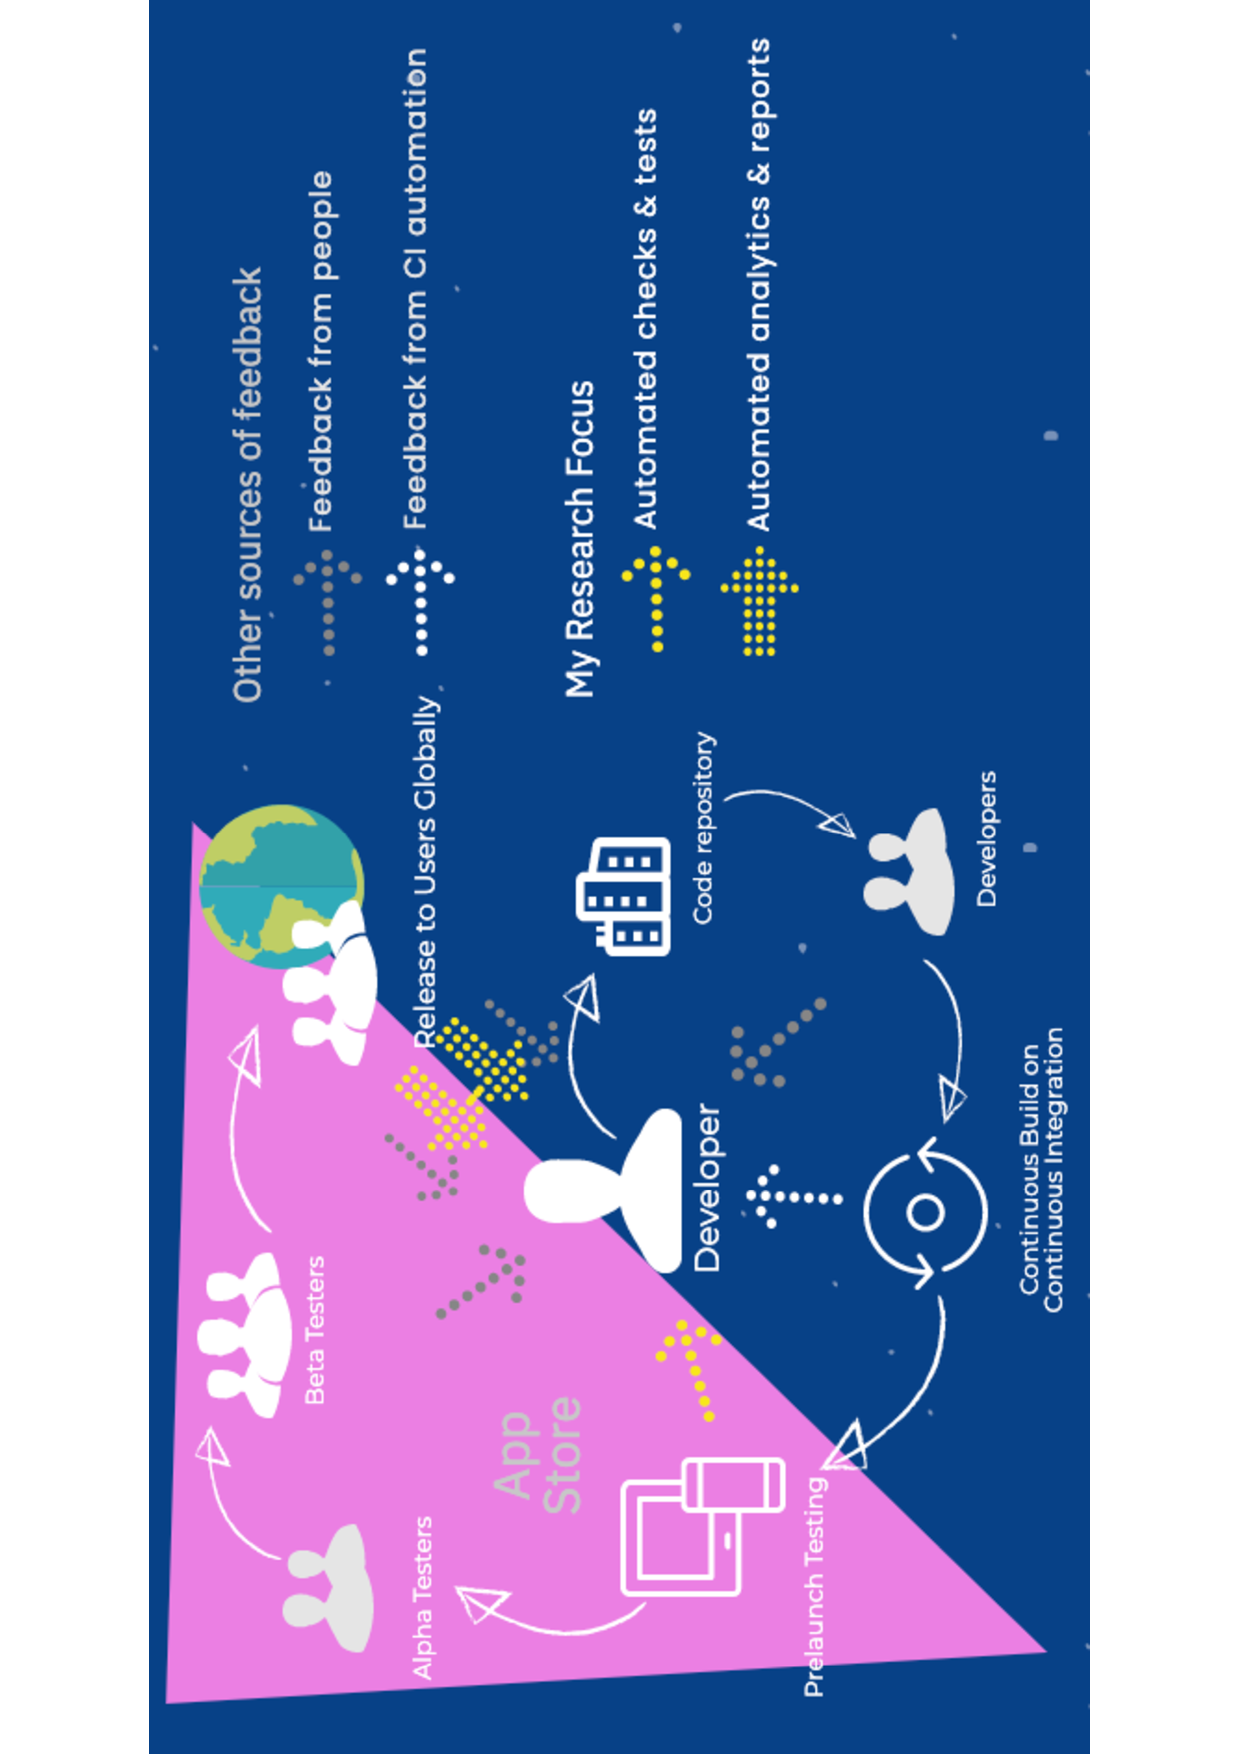
\includegraphics[width=\linewidth]{images/mobilesoft/silvias-developer-centric-figure-mobilesoft2020.pdf}
    \caption[Sources of feedback for developers]{Sources of feedback for developers \\The Research focuses on automated checks and tests performed by the app store, automated analytics and reports both in-app and at the platform level. \\ \\Other sources of feedback available to developers includes feedback from people and feedback from their development tools and CI automation.}
    \label{fig:sources-of-feedback-for-developers}
\end{figure*}

% TODO if the following footnote is split across 2 pages then review https://texfaq.org/FAQ-splitfoot to prevent an entire page becoming a hotlink for the URL in the footnote.
Developers have various sources of feedback about their apps, as Figure~\ref{fig:sources-of-feedback-for-developers} illustrates~\sidenote{Image created in pikochart \url{https://create.piktochart.com/teams/16497973/infographic/saved/47760961?}, a paid for online editing tool. Thanks to Silvia Harty for her help designing the original figure.}. The pink triangle represents the extent of Google Play (the app store) in terms of providing feedback. Other feedback is also available independently of the app store, for instance: from the development process, and by using software incorporated directly into the app that provides bi-directional communications between the development team and end users~\sidecite{avellis_harty_yu_towards_mobile_twin_peaks}.


Each source of feedback may stem from humans (for example, in reviews) or from software (for example, from code quality tools such as Lint).This research introduces three sources of software-generated feedback:
\begin{enumerate}
    %\setlength\itemsep{-0.5em} %\itemsep0em 
    \item Prelaunch testing: automated checks and testing provided by the app store (Google Play),
    \item platform-provided analytics: automated analytics and reports gathered by the Google Android platform from users devices configured to provide the underlying data,
    \item in-app error reporting (including crash reporting): software added by the app development team to detect and report crashes, and optionally errors and similar/related data.
\end{enumerate}

% NB: Alpha and Beta channels formed part of one of the major industry case studies. Clearance has not yet been granted to write or publish the findings.

Note: while the first two of these sources use Google Play as their source, other app stores and similar ecosystems may provide equivalent sources of feedback.

\section{Research Questions}
\label{section-research-questions}
%%%%%%%%%% Isabel Evans suggests adding a table with my RQs at the start of this section. TBD. COULD-DO. Certainly it seems this section needs polish.

%MUST-DO \yijun{If possible, you may need to dig out a few MobileSoft research papers to give evidence that these research questions have not been addressed in literature, e.g., \emph{Future Trends in Software Engineering Research for Mobile Apps}~\sidecite{nagappan2016_future_trends_in_sw_eng_for_mobile_apps}, whether the future work of some paper suggests one does not know the sources, value, or impact of mobile analytics to assess and improve app quality? Is there nothing in the general SE literature studying the "analytics" to "general software quality" problem? If there are such general work, how does "mobile analytics" and "app quality" differentiate the RQs to existing ones...}


My research hypothesis is that using mobile analytics can help improve the work development of teams and the quality of the products they create. Here work includes the development, testing, and bug investigation of the software being created. For the quality of the product, this research is focusing on a subset of qualities which are \gls{glossary-technology-facing}, %technology-centric, 
and in particular the \gls{glossary-reliability} and \gls{glossary-stability} of the mobile apps when they are in use. This research builds on prior work on software analytics for mobile apps and focuses on its practical application by software development teams to improve app reliability. This is important because app reliability, as measured by crash rates and ANRs, is key metric in the mobile app ecosystem. Because this metric is used by the platform provider to determine whether an app should be given access to the ecosystem, it is something developers should pay attention to. In order to understand the effect of applying mobile analytics on the software development practices for improving reliability of apps, we need to explore the processes, artefacts and tools associated with these activities. This research investigates these three dimensions based on case studies of different mobile app projects, to identify both the current practices and opportunities for improvement provided by using mobile analytics.

The core question investigated by this research:

\begin{quote}
  \emph{How can applying mobile analytics in software development practice improve the reliability of mobile apps?}~\label{overall-research-question}\index{Research questions}
\end{quote}
% Thanks to https://tex.stackexchange.com/questions/35933/indenting-a-whole-paragraph

To expand on the research question:
\begin{itemize}
    \item \textbf{Applying mobile analytics}: is the use of mobile analytics in order to effect improvements to the practices and the artefacts. Applying mobile analytics refers to both collecting data from the usage of the app and also making use of the analysis of this data to identify and address issues that can improve the app. Improvement of the app focuses on increasing the stability/reliability by reducing ANRs, crashes, and through improving how the app handles various errors (typically reported through Exceptions~\footnote{Exceptions are a core construct in Java programs intended to make those programs robust~\cite{robillard2000_designing_robust_java_programs_with_exceptions}, and similarly \glspl{glossary-exception} are core to Android apps}).
    \item \textbf{Mobile analytics}: Analytics where the data is collected by software running on mobile smartphone-based devices pertaining to the app's qualities-in-use. This research focused on analytics collected pertaining to the stability of the app, where stability includes the reliability of the app.
    \item Software development: includes tasks performed by the software developers including design, coding, testing, bug reporting, and bug tracking.  Use of Scrum development practices, following recommendations and guides that include application compatibility, \gls{ui} guidelines, and designing for performance and responsiveness, \emph{etc}. [Software] testing~\sidecite[][pp.398 - 399]{wasserman2010_software_engineering_issues_for_mobile_app_devt}.~\sidenote{This short paper skims over topics without evidence developers actually do them. Their survey, cited in this paper isn't available so appears to have not actually been published.}
    \item Reliability and Stability are two intertwined measures of software quality in use. There are contradictory opinions on their relationships to each other and to their contributions to software quality, these will be discussed in Chapter~\secref{chapter-related-work}. 
    \item In practice: the key scope of measurement focuses on the efficacy in real-world projects from the perspective of software practitioners who develop mobile applications.
\end{itemize}

In order to answer this research question it is appropriate to consider improvements to the \emph{app i.e. the product} and to the \emph{processes/practices} development teams apply when they develop and maintain their mobile apps. Improvements cannot be be usefully considered in isolation, they need to be grounded in the current practices: the developers will have their perspectives on their use of mobile analytics, and their development artefacts may provide cross-verification of what they say they do compared with tangible evidence of how they use those mobile analytics tools. 

Furthermore, there may be constraints and/or limitations in the current mobile analytics tools which may adversely affect the improvements development teams are able to make to their processes/practices and to their products, hence it is also germane to consider improvements to the current mobile analytics tools.

These additional supporting questions can be restated as six distinct yet related perspectives.

\begin{figure*}
    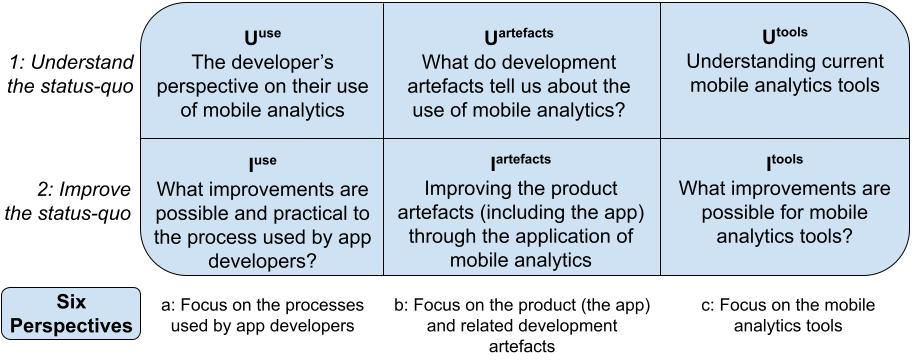
\includegraphics[width=\linewidth]{images/my/six-perspectives-2x3-matrix-12-nov-2021.jpeg}
    \caption{Six Perspectives of Mobile Analytics}
    \label{fig:six-perspectives-in-the-research-questions-section}
\end{figure*}

\subsection{Research questions lead to six perspectives}~\label{rq-leads-to-six-perspectives}
The six perspectives are illustrated in Figure~\ref{fig:six-perspectives-in-the-research-questions-section}~\sidenote{Source figure:~\href{https://docs.google.com/drawings/d/1SafKu3uqgl-s8-I8iWSSWmFY4NdlNpw8v6ZiJDGh50c/edit?usp=sharing}{Google Docs: Six Perspectives drawing}.} and paraphrased below:

\begin{enumerate}
    %\setlength\itemsep{-0.5em} %\itemsep0em
    \item [1a] What do app developers say they do in terms of using mobile analytics? (understand the \emph{status quo} from their perspective).\index{Research questions}
    \item [2a] What's possible in terms of improving their processes, their practices through using mobile analytics?)
    \item [1b] What does their source code (and other available development artefacts) tell us about their use of mobile analytics? (\emph{i.e.} to understand current behaviours in terms of the code that's implemented.
    \item [2b] What's possible in terms of improving the product (and particularly the mobile app) through the application/use of mobile analytics?
    \item [1c] What do we learn about various current mobile analytics tools?
    \item [2c] What improvements are possible for mobile analytics tools based on what was learned in the various case studies?
\end{enumerate}

These provide clear grouping for each of the three columns: on processes (a), on apps and related development artefacts (b), and on the analytics tools (c) which are considered in terms of first understanding and then improving the \emph{status-quo}, shown as two rows, \emph{i.e.} a 3x2 matrix. 


% https://www.skmurphy.com/blog/2014/01/27/difference-between-a-hypothesis-and-an-assumption/
Here the hypothesis is that analytics can help, as stated by Buse and Zimmermann ~(\citeyear{buse_analytics_2010}); and \emph{``with explicit and implicit feedback now available (almost) continuously, questions arise. How can practitioners use this information and integrate it into their development processes [to decide when to release updates]?"}~\sidecite{maalej2016_towards_data_driven_requirements_engineering}.


\section{Research contributions}
Before this research little was known about developers integrating mobile analytics into their artefacts and/or their processes. Unknown were - how, why, and when, they used the outputs of the mobile analytics. Similarly, the effects of using mobile analytics in terms of any changes to the reliability of these apps was not known. Furthermore, little was known about the mobile analytics tools and services used by app developers in industry or in real-world mobile apps.

\subsection{My contributions to knowledge}
The research contributes to the understanding of tools and information seldom available to research - of professional app developers, their artefacts, and of professional mobile analytics tools and services. 

\newthought{Processes}: 
My research contributes knowledge on the approaches various app development teams apply when they use mobile analytics including the selection, integration of code and services, and their application of mobile analytics to detect, identify, and address errors and failures reported by mobile analytics. It builds on prior research, for example, on Insight, and confirms their findings. It contributes new knowledge in the adoption platform-level and commercial in-app mobile analytics, including a) usage patterns by development teams ranging from individual  developers, small teams and large,  \gls{glossary-sharded}\sidenote{\href{https://en.wikipedia.org/wiki/Shard\_(database\_architecture)}{Wikipedia: Shard (database architecture)}} teams, and b) public opensource projects, hybrid projects that combined private and proprietary practices, through to a development team at a major corporation.

Some of the findings were surprising in terms of the patterns of use and in the efficacy of using mobile analytics to achieve significant improvements.

Development teams who embedded mobile analytics into their ongoing, core practices, were able to achieve highly reliable and stable apps. 

\newthought{Artefacts}: 
The research extended prior art in studies of opensource mobile app codebases, with a focus on the use of the most popular product offering: Firebase Analytics. Developers often incorporated multiple mobile analytics libraries into a single mobile app, each for a specific purpose. When developers addressed failures reported by mobile analytics they often modified the source code of the app; these modifications were generally small, yet the effects on improving the reliability/stability of the app were material. 

It also contributes insights from proprietary, commercial codebases and issue tracking artefacts where development teams intermittently filed bug reports for issues reported by mobile analytics.

\newthought{Mobile  Analytics Tools}:
The research identified characteristics of a wide range of mobile analytics tools that serve Android app developers in particular. It also found and  presents a range of flaws found in professionally-developed mobile analytics tools, including several of the most-used mobile analytics offerings.

The research contributes material relevant to professional app developers and to the developers of mobile analytics. 

Improvements were identified in all three areas and some of these were implemented during the research. 

Note: In addition to specifying my research contributions add explicit summaries of my contributions that have already been published.

\subsection{Practical impact of my work}
Several of the tool development organisations including Amplitude, Google, and Iteratively actively sought insights and updates from my research. They improved various aspects of their respective mobile analytics offering.

App developers who applied the techniques described in my research were consistently able to significantly improve the reliability/stability of their apps.


\section{Outline of this thesis}
At a high-level thesis is in three main parts: the preamble which includes chapters 1 to 5, the findings in chapters 6 to 8, followed by the discussion, conclusion, and future work in chapters 9 and 10. There are two short appendices: on thematic analysis, and additional details for some of the mini-experiments.

\bigskip

This thesis starts with an introduction to the context of investigation - mobile app development - together with an exploration of the state of the art. Based on this, the method adopted for conducting the research is presented before outlining the different mobile app and analytics tool case studies. Following this, the findings are set out, covering three thematic areas relevant to the use of mobile analytics: app development processes and the use of analytics, apps and their artefacts, and mobile analytics tools. Finally there is discussion of the findings together with potential areas for future work. A more detailed outline of the remaining chapters of the thesis is set out below.

\newthought{Chapter 2 | Preparing the ground:} this chapter prepares the ground for the rest of this thesis by explaining contemporary development practices for mobile apps. It then presents five conceptual models related to mobile apps. These are followed by several, relevant, practical details.

\newthought{Chapter 3 | Related work:} explores the state of the art relevant to software quality, software analytics, and the mobile app ecosystem.

\newthought{Chapter 4 | Methodology:} sets out the research approach adopted to gather and analyse data for the different case studies explored as part of the research.

\newthought{Chapter 5 | Overview of the case studies:} introduces each of the app-centric and tool-centric case studies using a consistent structure to make them easy to comprehend and to facilitate comparison.

\newthought{Chapter 6 | Findings - Analytics in use:} presents the key findings from the case studies relevant to the use of analytics by mobile app development teams.

\newthought{Chapter 7 | Findings - Apps and their artefacts:} discusses the findings relating to the software developed in the different mobile app case studies, together with their associated artefacts.

\newthought{Chapter 8 | Findings - Mobile analytics tools and their artefacts:} Focuses on the mobile analytics tools explored during the course of the research and the different artefacts produced by these tools.

\newthought{Chapter 9 | Discussion:} Explores the findings across the different perspectives of the research in relation to the wider literature of software quality and mobile app development practices.

\newthought{Chapter 10 | Conclusions and future work:} Summarises the key contributions of the research and discusses avenues for further investigation.


% Temporary removal to try and short-circuit compile timeouts
%\chapter{Preparing the ground}
\label{chapter-preparing-the-ground}
\emph{`...there is nothing new under the sun. \\Is there anything of which one can say,``Look! This is something new"?'}~\sidenote{\href{https://www.biblegateway.com/passage/?search=Ecclesiastes+1\%3A9-10&version=NIV}{Ecclesiastes Ch:1 vv. 9-10 NIV edition.}}

\setkeys{Gin}{draft}
\julian{This chapter is currently in draft compilation mode to try and stop timeouts on Overleaf. See \url{https://www.overleaf.com/learn/how-to/Optimising_very_large_image_files} for details.}
\vspace{10mm}

This chapter provides a grounding in the domain of mobile apps, how developers obtain information, and mobile analytics,~\emph{etc.}  
% MUST-DO revise opening sentence and remove the etc. via \akb
For any individual elements there may be much that is known and seemingly little novelty. And yet, it has become clear that when these elements are combined an interesting and rich domain emerges that can serve developers of their mobile apps.

While this discussion of the mobile app ecosystem aims to be as detailed and accurate as possible, there are limits to which this is possible in the context of closed, proprietary systems including those discussed in this thesis. 

To improve readability the thesis includes some generalisations rather than using qualifiers throughout, such as often, mainly, and so on, unless they materially reflect variations in people's experiences.

The chapter introduces five 
%MUST-DO revise this and the next paragraph once the chapter's contents have settled down.
conceptual models, including: a model of apps and app stores, layers of an app and observation points, of analogue and digital feedback, usage analytics, and finally DevOps. These concepts help us understand key considerations for mobile app developers and what they are working with.

The chapter continues with five practical aspects including app development and usage, information sources for developers, and choices for engaging with analytics. Developers need to address these as part of being effective in their work and providing apps of adequate quality. Mobile analytics can provide useful sources of information, including problems with the apps in use, and mobile analytics can complement and calibrate other sources of quality related information including software testing. 


\section{Potential sources of evidence}~\label{sec:potential-sources-of-evidence}
\emph{Note: this was moved from the Introduction and may have a better home. \textbf{MUST-DO} integrate this section in this chapter.}
%\emph{What can we learn from people? what can we learn from analytics? ...?}

%\textbf{How can we know about mobile analytics and the effects of using them?}

%\nth{16} Jul 2021:~\akb{This subsection is too verbose. Summarise with a diagram showing sources of knowledge and links to difference types} - \textbf{MUST-DO} and will do once I make sense of where's the best place to put this material. For now I've moved the overall \href{section-ontology-and-episetemology}{\nameref{section-ontology-and-episetemology}} section to after the RQs and before the methodology section.

%Here we consider the questions: (1a) What we can know about mobile analytics and (1b) how we can know it? Then more specifically, these related questions are key given this research focuses on using mobile analytics to help answer the next question. (2) How we know about the identification and measurement of some flaws in behaviour of software that are considered measures of quality of the software in use?

Broadly we can learn from people, use \textit{software analysis tools}~\sidenote{MUST-DO add a paragraph on software analysis tools.}, and use data to answer these questions. In some cases the data comes from a single source, in others cases from several.

\textbf{Software analysis tools} 

Lint~\sidenote{\href{https://developer.android.com/studio/write/lint}{Android Lint} or \href{https://github.com/realm/SwiftLint}{SwiftLint} for iOS.}


\textbf{Mobile analytics} comprises software, systems, and sometimes services. Broadly we can read about them, study their source code, analyse, test, and use them directly, and ask others for their perspectives and insights. Rather than go into lots of detail here, several of the appendices of this thesis cover aspects of mobile analytics, in particular, in~\href{app:on-mobile-analytics}{\emph{\nameref{app:on-mobile-analytics}}}.

In terms of learning from \textbf{people}, we can do so by asking the designers, constructors, operators, and users of a system. However, we're also limited by who we can ask, what they are willing/able to communicate, and whether that communication is sufficiently open and transparent to be useful and reliable. We can also learn from information produced by people, and in particular for mobile apps we can use ratings and reviews. Given human behaviour it may also be worth considering aspects such as the provenance of the information sources, fake data, \emph{etc.} especially where there are rewards for slewing the results of the measurements being used in an ecosystem.

We can know through \textbf{static analysis} tools, automated tests, end-to-end testing, \emph{etc.} and all of these are used by at least some of the developers of mobile apps some of the time. They often take place \textit{before} the software is released to end users.

We can also know through data collected when the software is used. As~\sidecite{RFC3164} notes in RFC3164, ~\emph{``Since the beginning... operating systems, processes and applications were written to send messages of their own status, or messages to indicate that certain events had occurred. These event messages generally had local significance to the machine operators."}. Mobile apps also write messages locally and developers use them for similar purposes (nuances and differences are discussed in the related work chapter). These local messages can be read by humans locally and/or read by software that delivers them elsewhere. Developers can also add software to their apps to log information for processing elsewhere which is where much of mobile analytics and crash reporting fits in the scheme of things.

Log messages are written locally on the same device (\textit{i.e.} computer) that runs the software. When developers are developing the software they tend to be local to the device and therefore able to read the logs. When the devices are remote, as they are for end users of mobile apps, developers cannot easily access the logs or read them. If they wish to do so they need mechanisms to obtain the logs. They can choose to incorporate mechanisms into the app including custom logging mechanisms that transmit the logs so they can be processed remotely. They can rely on log forwarding software~\sidenote{For instance a fairly involved example for Flutter Android apps, using MQTT, is described in~\cite{adil2020_sending_logs_from_flutter_apps}}, and/or mechanisms provided on the device if they exist.
% A couple of Android implementations for LogStash include:
%  https://github.com/Labgoo/android-logstash-logger
%  https://gist.github.com/PatrykGala/55603fe4259d812fdc0ffbc9e63eaabc (saved in my references)


Various data can be potentially collected implicitly and explicitly. What can be collected depends on the observation mechanisms. Observation may be within an app or external to it, for instance by the operating system as both iOS  and Google Android do~\sidenote{There are other custom versions of Android, for instance used in Amazon Kindle Fire devices. Their details are outside the overall scope of this research.}(details in the Appendix titled~\href{chapter-on-mobile-analytics}{\emph{\nameref{app:on-mobile-analytics}}}). Within an app the observation may focus at a single layer, for instance the visual user interface, or several. The choices of observation mechanisms within an app are made by developers or their stakeholders. The choices external to an app can be made by various people including the platform provider, users, or indirectly using other software including third-party apps, spyware, accessibility software, and so on.

Analytics, such as user-journeys, can help to answer questions about the usage of the software. They help establish \emph{what-is}. As we understand more about what-is we can then consider \emph{what-would-be-better} and do gap analysis between what-is and what-would-be-better.

%See https://tex.stackexchange.com/questions/348298/svg-package-includesvg-with-underscores-in-svg
\makeatletter
\DeclareRobustCommand*{\escapeus}[1]{%
    \begingroup\@activeus\scantokens{#1\endinput}\endgroup}
\begingroup\lccode`\~=`\_\relax
    \lowercase{\endgroup\def\@activeus{\catcode`\_=\active \let~\_}}
\makeatother

%See https://tex.stackexchange.com/questions/390804/how-to-scale-text-in-svg
% PS: I could try https://tex.stackexchange.com/questions/113282/text-size-in-inkscape if I run into problems with the current approach.
\begin{figure*}
    \copyrightbox[r]{
        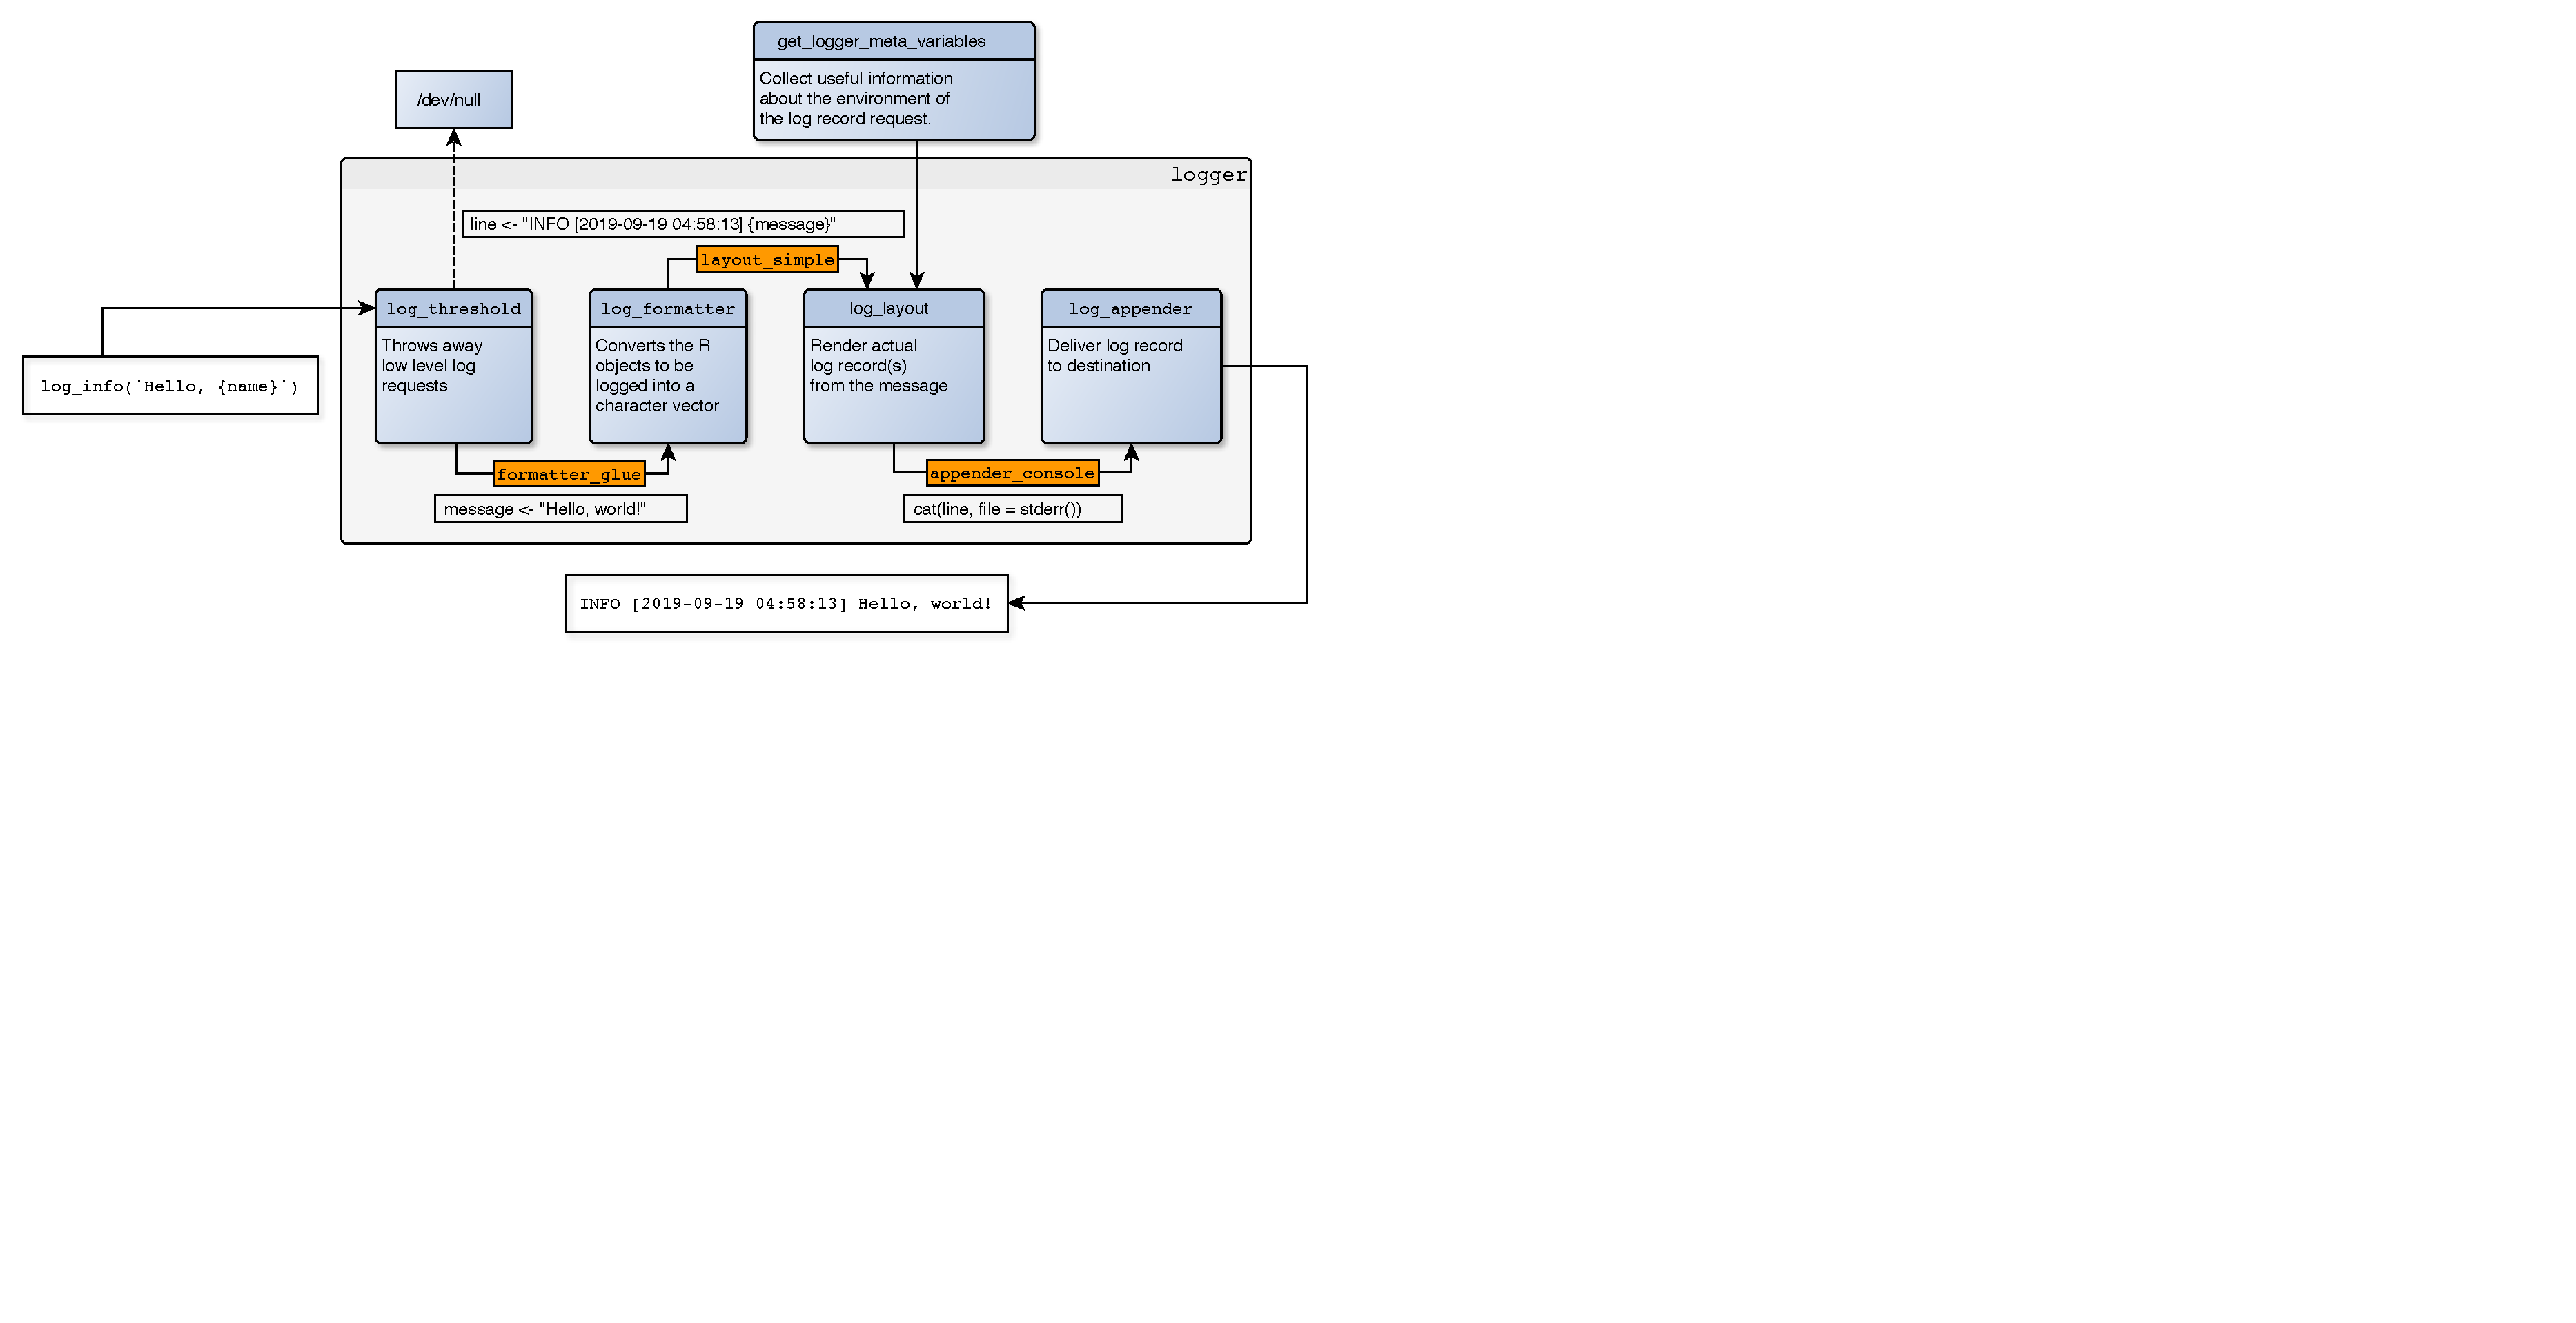
\includegraphics[width=\linewidth]{images/github/loggerstructure.pdf}}
    {\textcopyright \href{{https://twitter.com/daroczig}}{daroczig}\\source: \href{https://github.com/daroczig/logger/blob/master/vignettes/logger_structure.svg}{logger\_structure.svg}}
    \caption{TEMP - to be replaced: Logger Structure from an R Logger project - TBC whether to provide something similar}
    \label{fig:temp_logger_structure}
\end{figure*}

\begin{comment}
%This is a simpler structure without the copyright box. Commented out for now, kept in case I want to switch quickly.
\begin{figure*}
    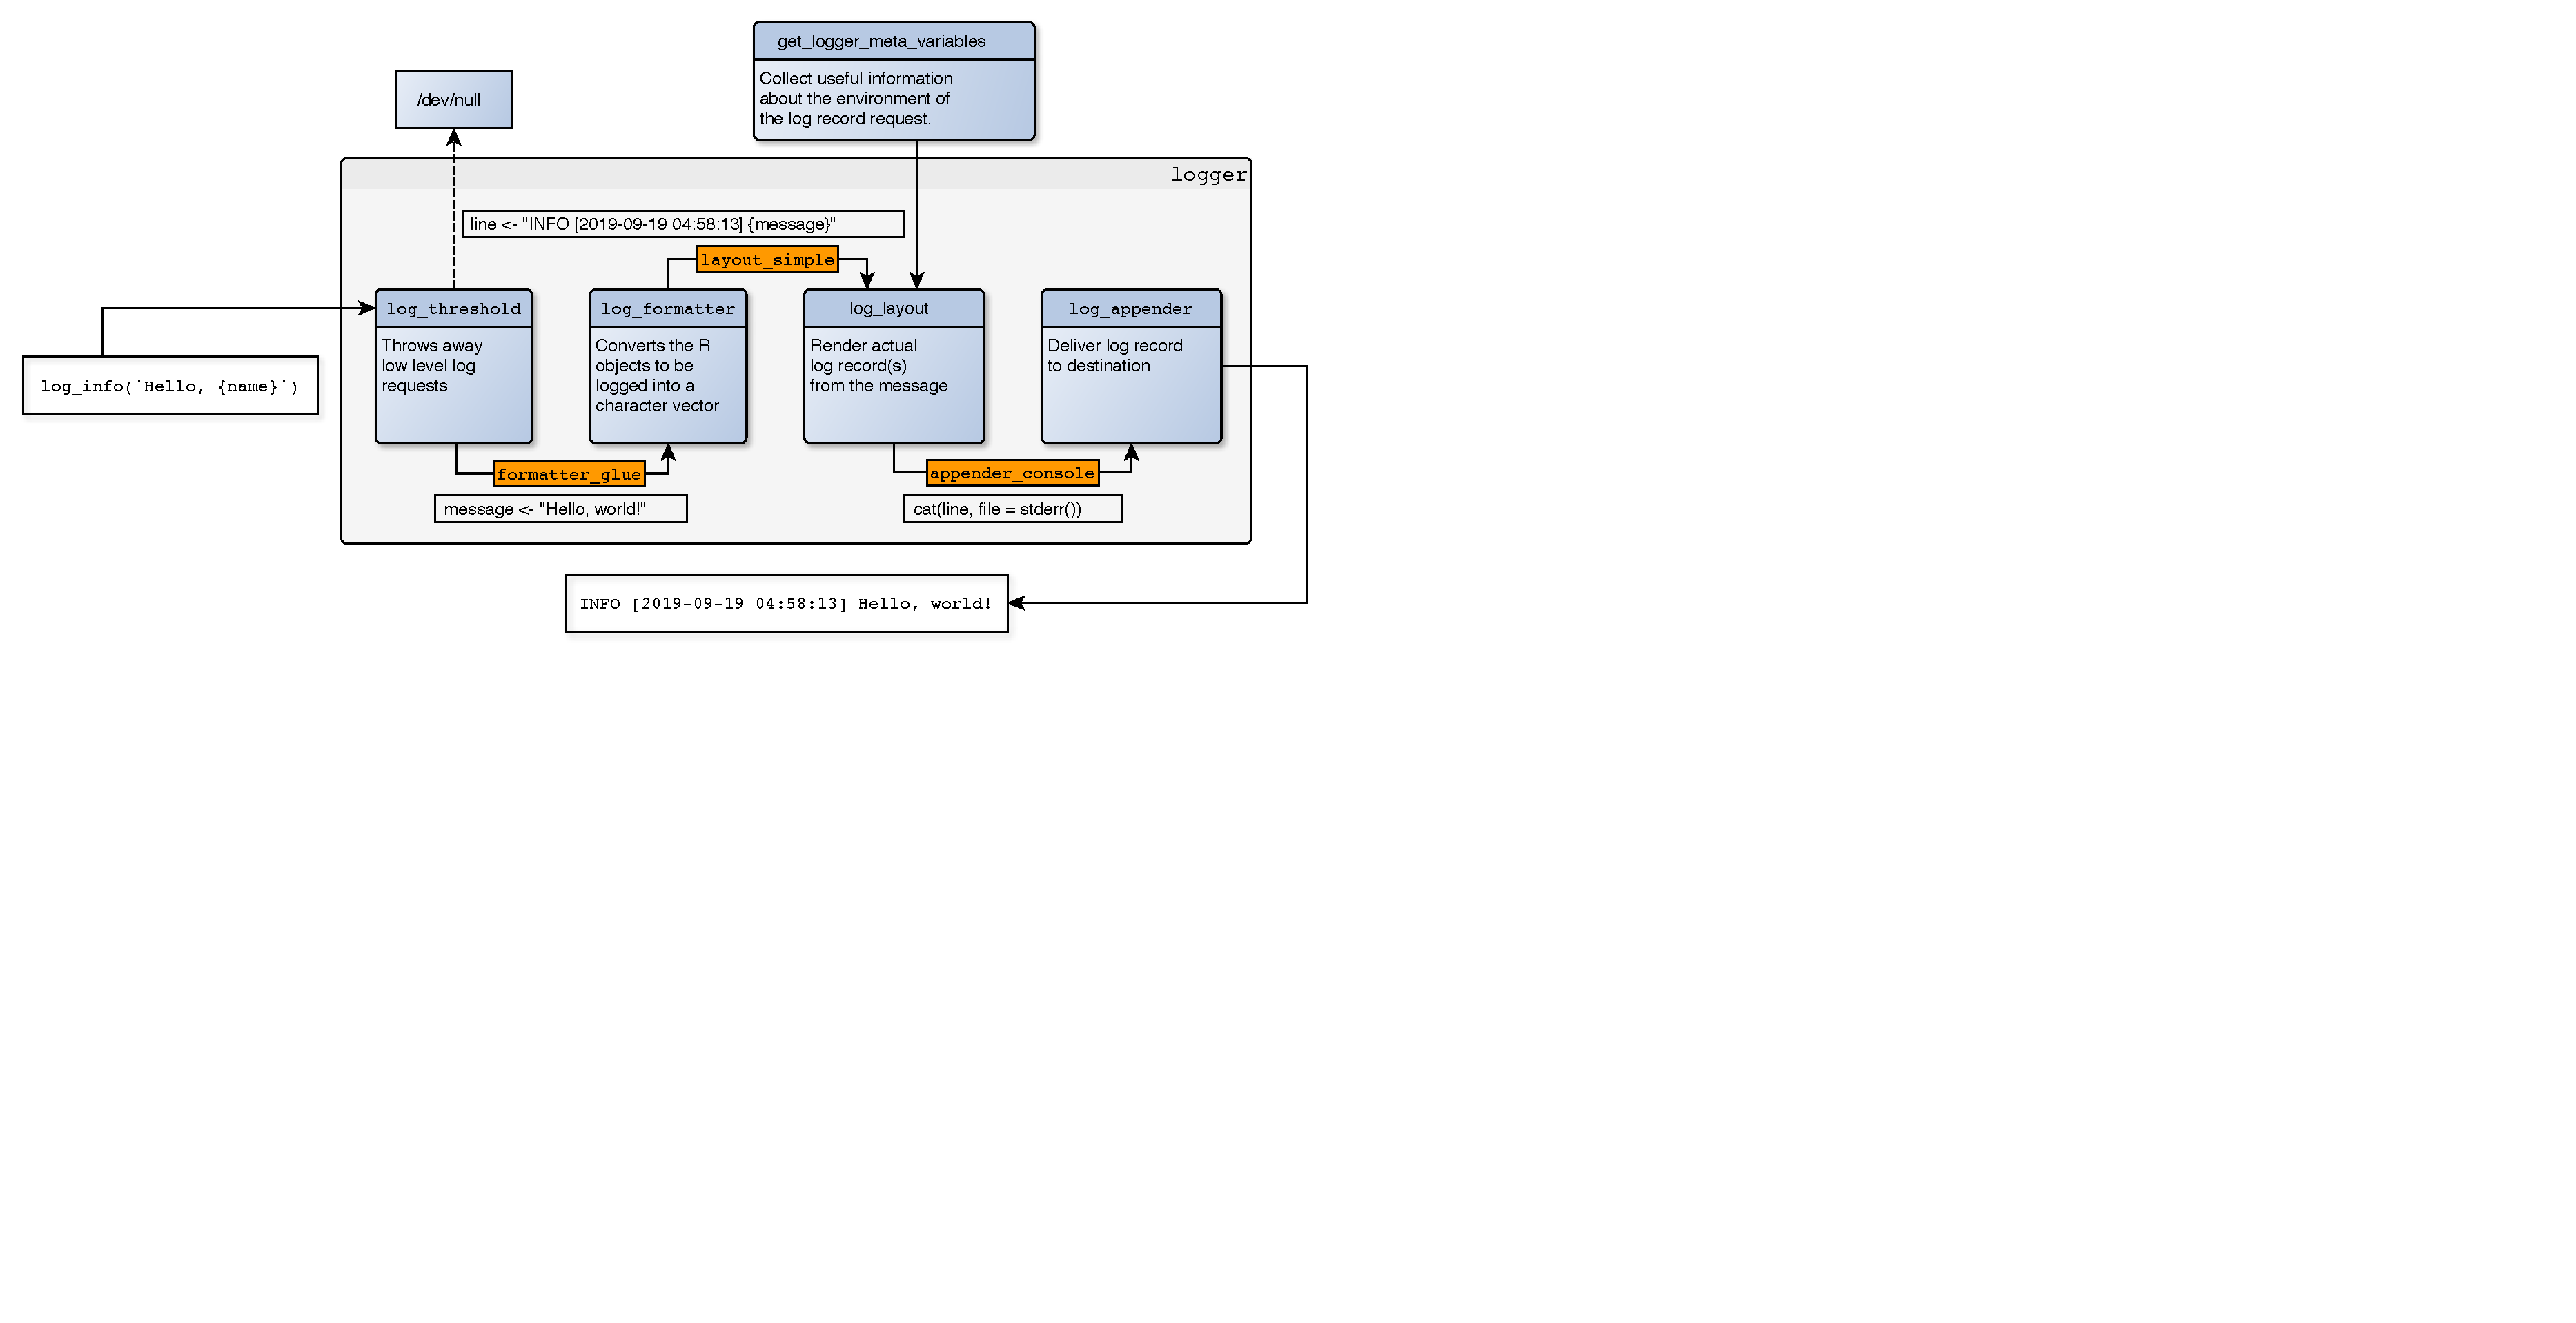
\includegraphics[width=\linewidth]{images/github/loggerstructure.pdf}
    \caption{Yin Yang to represent DevOps}
    \label{fig:yinyang_for_devopsxxx}
\end{figure*}
\end{comment}


\textbf{Reporting/generating and Observing}: What happens within the app stays within the app unless someone looks inside the app or the app reports what's occurring. Observation without action limits the utility of whatever is learned.  \textbf{SHOULD-DO}, it'd be great to have a figure similar to \url{https://github.com/daroczig/logger/blob/master/vignettes/logger_structure.svg} for platform-level analytics. Temporarily it's included here in Figure~\ref{fig:temp_logger_structure}.


Survivorship bias (\sidecite{wikipedia_survivorship_bias}) is relevant to understanding the information developers receive, some data does not `survive' the journey from source to developer. And much of the information that is does reach the developers does not survive or, perhaps better put, thrive in terms of being used productively. They have plenty of other demands for their time and attention and much of what could be useful isn't used in practice, therefore the data needs to be sufficiently useful and relevant and improvements tractable for any proposed approach to be used long term in practice.


Discuss which sources are likely to provide input to the key elements needed to underpin the RQs.

\textbf{MUST-DO} Segue to the research strategy and how we devise a feasible approach that uses as many of these sources as practical.



\section{Development practices for mobile apps}
Few if any developers write perfect software, and this applies also to developers of mobile apps. 

%SHOULD-DO Add the Amphitheatre illustration. And suitable words to explain the concepts.

This section introduces the concept of \textit{Zones} as they apply to finding and potentially fixing issues while developing software. The concepts are inspired by various sources including agile development practices, release management for mobile apps, computer networks, and particularly the use of firewars and `de-militarised-zones' (known as DMZ). 

\subsection{Control (find-fix) zones}
A find-fix Zone incorporates the scope of finding issues and being able to fix, or at least ameliorate, them. Where issues are discovered in the local Zone, developers can fix the issue without needing to involve others (however they can choose to do so), and indeed some may consider these issues an intrinsic and essential part of iterative software development. Other zones extend beyond the immediate developer and involve other people.

For the purposes of my research I have identified three categories of zones:
\begin{enumerate}
    \item \textbf{Local Zone}: This is local to the developer of software, tests, resources, designs, and so on.
    \item \textbf{Mezzo Zone(s)}: These zones involve other people, they may be peers, team members, other people in the organisation, trusted testers, and so on. There may be anything from virtually no zone for solo independent developers working on their own app, to a plethora of zones involving various stages of pre-release testing, checking and approvals in large corporate organisations.
    \item \textbf{Live Zone}: End users are able to use the released app. The app is finally able to potentially achieve business objectives. 
\end{enumerate}

\begin{figure*}
    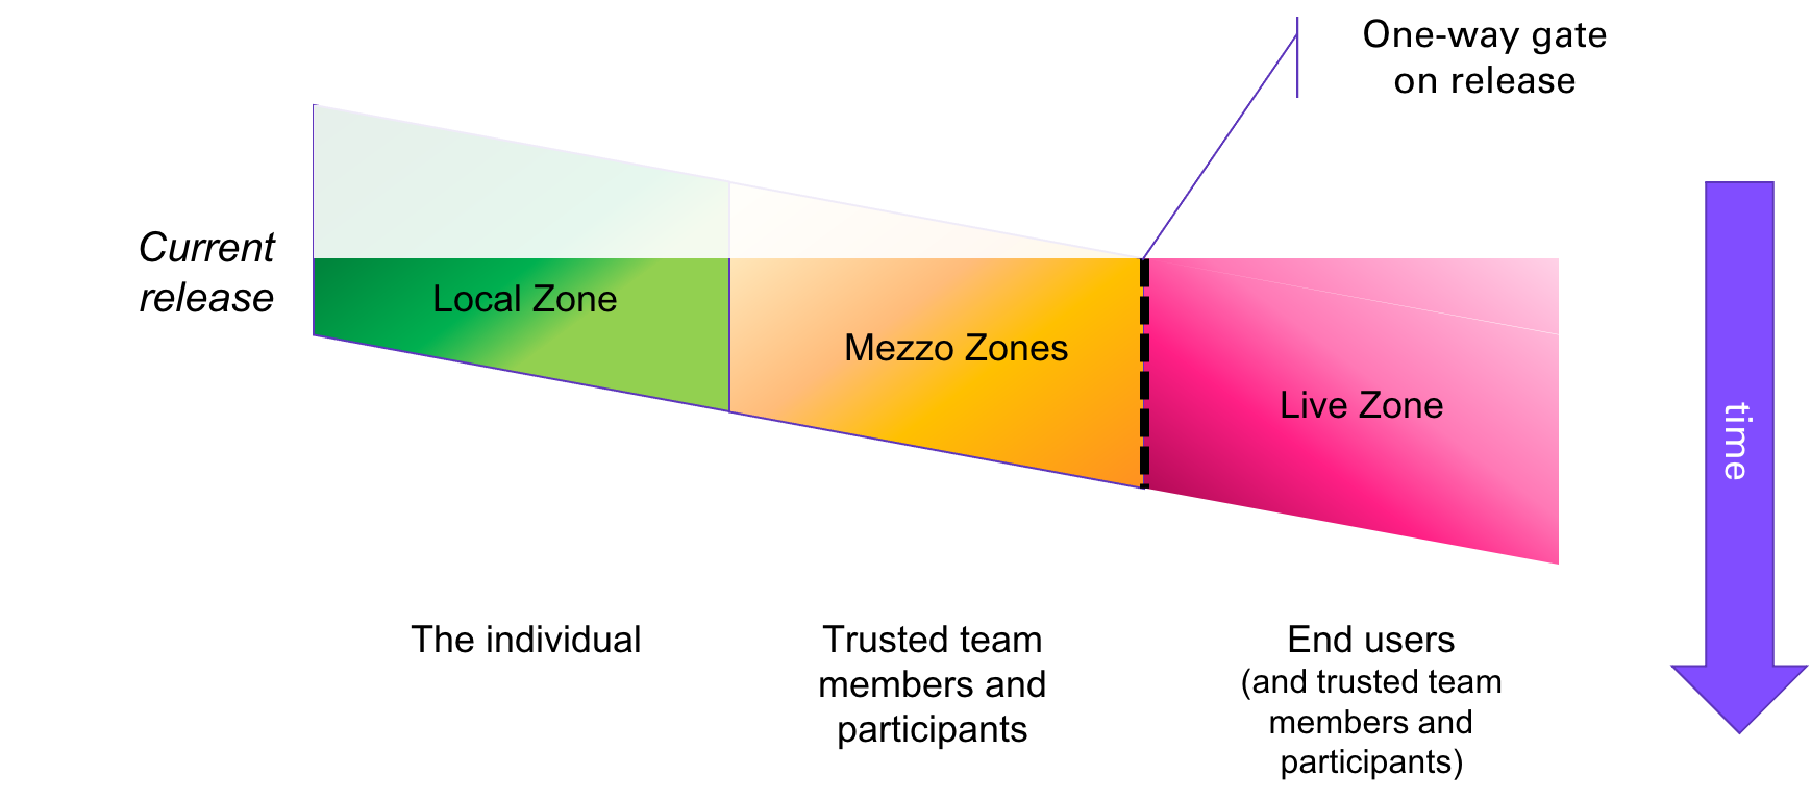
\includegraphics[width=\linewidth]{images/my/control-find-fix-zones-a.pdf}
    \caption{Control find-fix zones}
    \label{fig:my:control-find-fix-zones-overview}
\end{figure*}

These three categories of zones are illustrated in Figure~\ref{fig:my:control-find-fix-zones-overview}. The figure includes a one-way gate, that behaves like the Rubicon in Julius Caesar's time~\sidecite{wikipedia_rubicon} where the die is cast once a release has been launched in the app store. The release cannot be reverted, at best it can be paused or superseded with another subsequent release. The app now comes into contact with end-users and is expected to achieve the business objectives of the organisation who made it available.

\begin{figure*}
    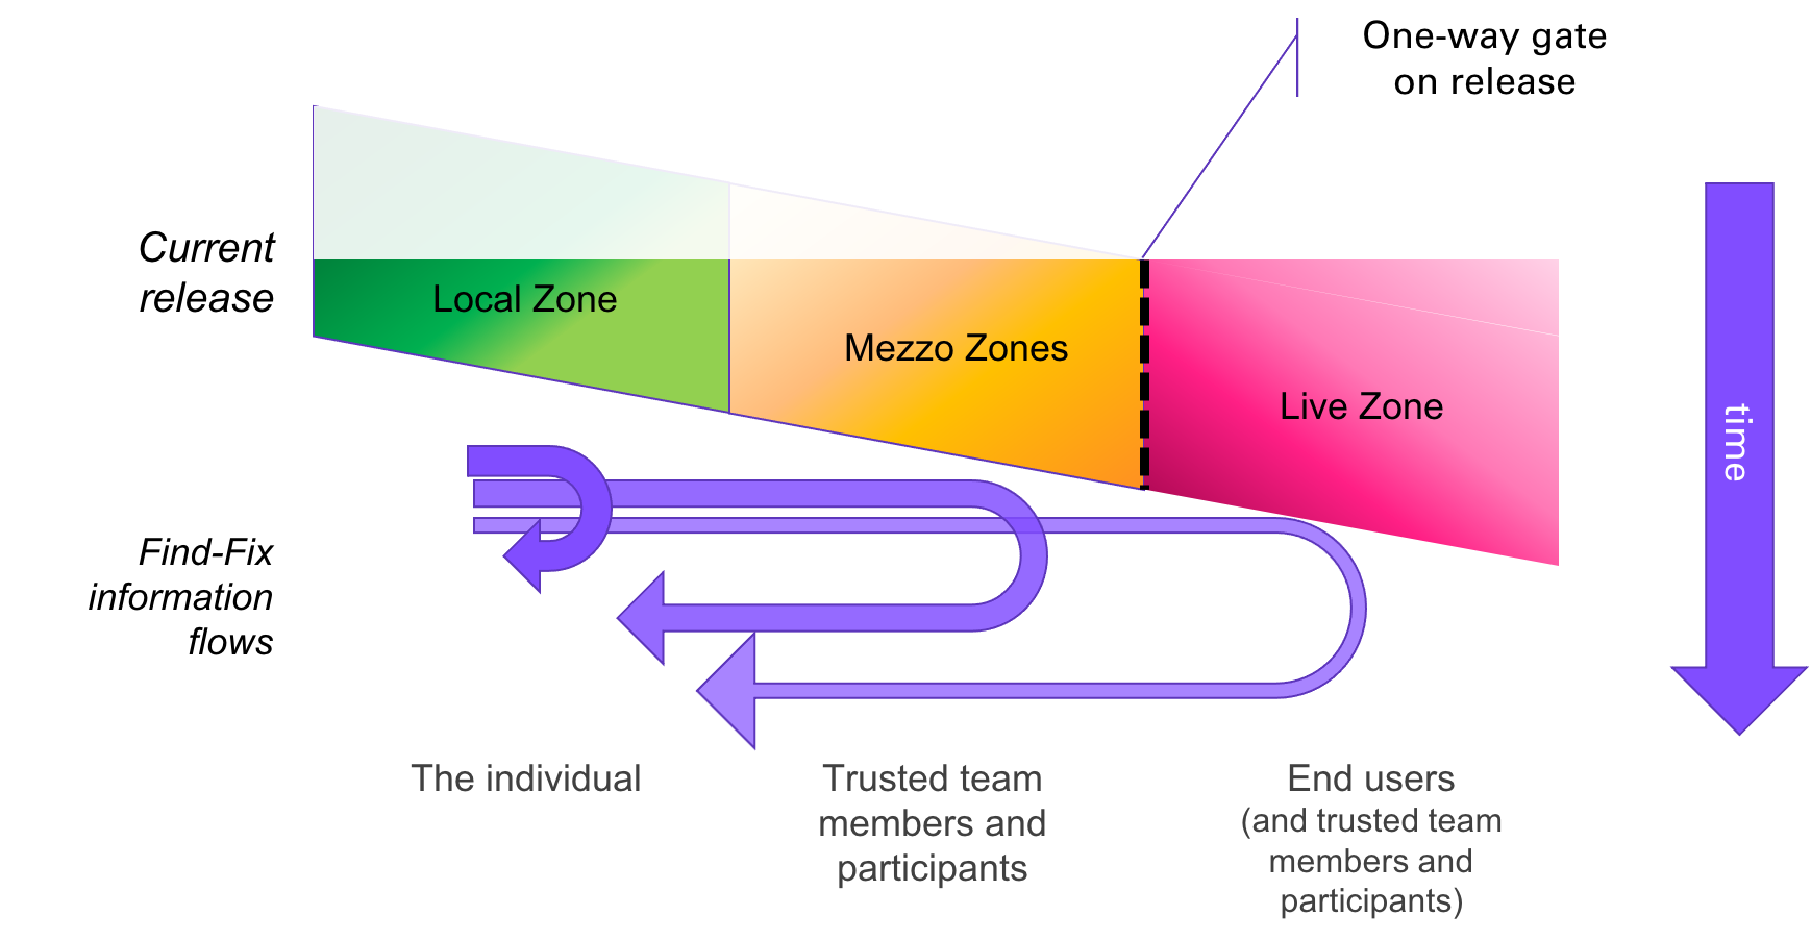
\includegraphics[width=\linewidth]{images/my/control-find-fix-zones-with-information-flows.pdf}
    \caption{Control find-fix zones with information flows}
    \label{fig:my:control-find-fix-zones-with-information-flows}
\end{figure*}

Figure~\ref{fig:my:control-find-fix-zones-with-information-flows} is a modified version of Figure~\ref{fig:my:control-find-fix-zones-overview} that includes the find-fix information flows. Assuming fixes are made be the development team for the app (rather than improvements that can be addressed in servers, through configuration changes, and so on) then the information about flaws and issues needs to reach that development team somehow. For issues found in external releases (\emph{i.e.} those made available to end-users) 

When issues are discovered before the software is released there is the possibility of the developer being able to address them before the software is released (they stakeholders may choose to delay the release to allow this to happen). Where issues are discovered in the released app, unless there are viable mechanisms to patch the app, the fix needs to be made in a subsequent release \textit{and} the end-user needs to use the subsequent release to receive the benefit of the release.

There are two key challenges:
\begin{enumerate}
    \item the developer learning about issues in sufficient detail to potentially address them,
    \item being able to address issues and provide the benefit to users who are, or  may be, affected by it.
\end{enumerate}

Both these aspects are covered next in terms of the bug-fix process for mobile apps.

\subsection{Bug-fix process for mobile apps}
%MUST-DO move the following comment to the next chapter once I've drafted the relevant illustrations.
% In my view, mobile analytics helps in the 'current' timeframe of the development and release process, in that it can provide ranked notifications of various issues (including 'stability' failures: i.e. crashes and ANRs) on a timely basis. 

Given apps have been released and users are using those releases then - there may be issues in the app exposed while it is in-use. Some of these may be noticeable (or perceivable) by the end-users, others not. These issues include 'stability' failures: \textit{i.e.} crashes and ANRs and performance-related issues \textit{e.g.} slow responses, excessive power and network consumption, and so on.

Sources of failures when an app fails a user include: code written by the developer or their colleagues (where they have control over the source code and can modify it as they see fit), third-party libraries (which are used extensively in mobile apps and where developers can replace, up- or down- grade the library but little else), or the platform, including platform-provided code.

For the development team to actively address any of these failures they need to be aware of them and have sufficient details to take action. Figure~\ref{fig:my:bug-fix-process-for-mobile-apps-in-prod} illustrates past, current, and future, activities for current and future releases of an app. We will return to this figure %in this section and 
in the next chapter where the effects of applying analytics to the development process is considered.
%MUST-DO make sure I do return to {fig:my:bug-fix-process-for-mobile-apps-in-prod} in the next chapter, on applying analytics.

\begin{figure*} %[!htbp]
    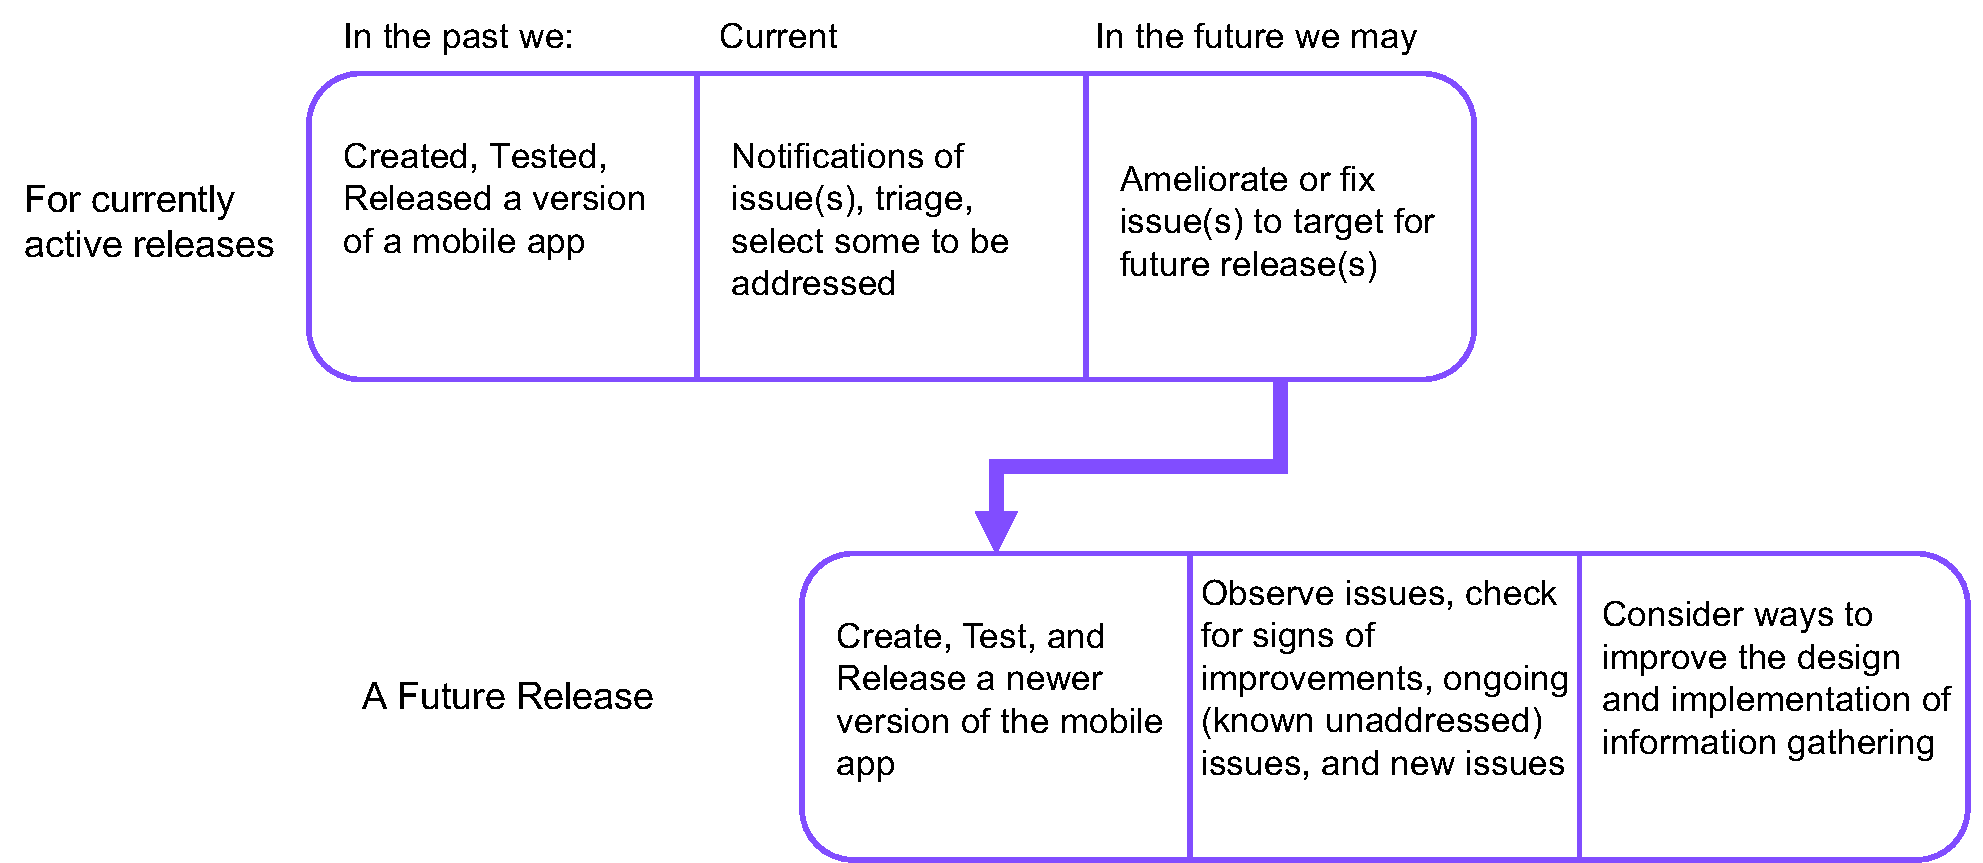
\includegraphics[width=\linewidth]{images/my/production-bug-fix-process-for-mobile-apps.pdf}
    \caption{Bug-fix, process for mobile apps in production}
    \label{fig:my:bug-fix-process-for-mobile-apps-in-prod}
\end{figure*}


Developers might learn of some of these issues from other sources e.g. from colleagues who use the app, from end-users who report issues (e.g. in reviews in the app store, on social-media, and even using in-app feedback if the app's functioning sufficiently etc.). 
% MUST-DO refer to research in automatically creating automated tests to reproduce crashes and discuss some of the limitations of that research vector. Note: this might be covered in the related works chapter.
However in my experience, and based on other research, only a subset of the issues are reported by a small subset of people who use the app~\sidenote{Estimated as 1\% by the company Raygun~\url{https://raygun.com/about}.} % Only 1% of customers actively report errors and performance issues they encounter whilst using web and mobile applications.
, and certainly not all users report all the stability issues all of the time. Google added a feature to Android 2.2 to enable users to easily send crash reports to Google which Google presented on the `Bugs' tab to the app developer~\sidecite{androiddevelopersblog2012_android_application_error_reports}.

Any amelioration or fix that occurs in the app's codebase is only useful to those users who use the newer release of the app that include the improvements. Our research confirms some users continue using older releases of the app unless blocked/prohibited from doing so (there are mechanisms for doing so). Blocking/prohibiting use of older failing versions of the app may be a mixed blessing. Some users may be lost and/or upset by being forced to upgrade the app. However the stability stats in the app store may improve (assuming the intended improvements were effective).


\section{Conceptual model of apps and app stores}
This section introduces a conceptual model of apps and app stores and presents four views of apps in an app store together with various implications of the views, relationships and interactions. 

The vast majority of mobile apps are provided through app stores, and the two largest app stores:~\href{https://play.google.com/store/apps}{Google Play} and Apple's~\href{https://www.apple.com/app-store/}{App Store} both collect mobile analytics from end user's devices with permission. So, understanding the conceptual model of apps and app stores provides some context for these sources of mobile analytics. 

The concept of an App Store has existed since at least 2003, according to the co-founder and CEO of Salesforce~\sidecite{benioff_trailblazer_2019}, where the idea was proposed by Steve Jobs and later implemented as \href{https://appexchange.salesforce.com/}{\emph{AppExchange}} in the Salesforce platform. Around the same period various app stores emerged for mobile apps~\sidenote{Tens of app distribution platforms are listed on Wikipedia:~\href{https://en.wikipedia.org/wiki/List_of_mobile_app_distribution_platforms}{List\_of\_mobile\_app\_distribution\_platforms}}; and the concept seems to have been introduced around 1999 by Handandgo~\sidenote{\url{https://en.wikipedia.org/wiki/Handango}}. Academic research into the effects of app stores emerged in or around 2010, for instance with the work of Kimbler who investigated the effects on mobile operators from a business strategy perspective~\sidecite{kimbler_app_store_strategies_2010} (mobile operators lost out in the overall battle of app stores, now platform specific app stores dominate the market). 

The research is situated in apps that are available in app stores and in the Google Play app store specifically. App stores house millions of apps and serve billions of users. They also present a rich tapestry of perspectives on software apps and the ecosystem. There has been a great deal of research that focus on particular areas of these apps and sometimes connect these areas as part of the research. This research focuses on an area seldom investigated, namely it concentrates on the developer's view of how their app is perceived by the app store and whether they can improve the perception by addressing sources of failures.

\begin{figure*}
    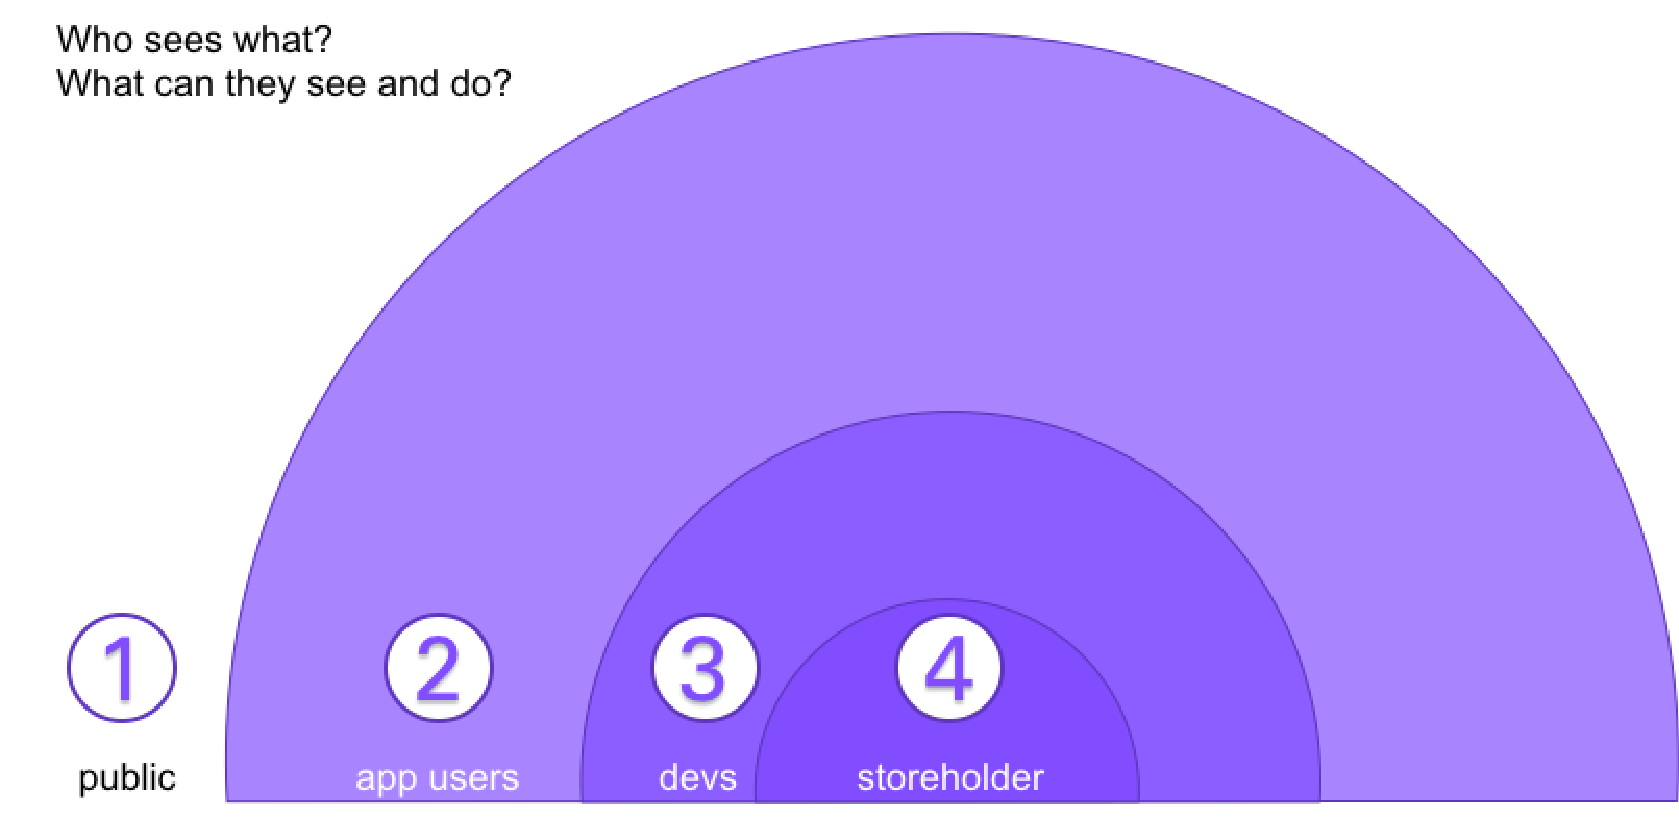
\includegraphics[width=\linewidth]{images/my/who-sees-what.pdf}
    \caption{Four Views of an App Store}
    \label{fig:4-views-of-apps-in-app-store}
\end{figure*}

Figure~\ref{fig:4-views-of-apps-in-app-store} illustrates the four views; broadly, those closer to the centre can also see what those in outer rings can see. As a wise supervisor commented: \emph{``It's a bit like standing at different elevations on a mountainside and looking out over the landscape - the higher you are, the more you can see"}.

The first view is the public view of the app store, what is visible to someone who is not actively engaged with the app store. Examples include people who are not logged into their account, search engines, researchers mining the app store for ratings and reviews, and so on. The public is able to see aggregate ratings and some recent reviews for specific apps. Older reviews are generally hidden from public view (which may limit some research and search engine insights).

The next view is that of a user of a particular app or set of apps. They may have installed some of the apps directly, they are likely to also have pre-installed apps on their device too. They have the ability to interact with the app store, for instance they can see, create, and update their ratings and reviews~\sidenote{If supported by the app store, for instance Google Play does.}. They can also see the public view.

%\akb{In the sentence below, does '.. records about their interactions ...' refer to the interactions of the developer or the user?}
Developers have the next view, which includes information the app store records about the developer's interactions with the app store, and information the app store provides the developers directly (\emph{i.e.} generated by the app store and related entities), as well as feedback provided by users via the app store (\emph{e.g.} ratings and reviews). Developers can also see the public view, although they cannot see the entire view of their user-base. However they can see any rating and reviews provided by the users.

%\akb{Do we know why the qualified 'often' is needed in the next sentence? Is this a non-deterministic behaviour of app stores and hence a forewarning of some of the data quality issues in the analytics platforms?}
Authors and developers are the two end points of ratings and reviews. Authors create them and developers receive them and can choose to respond to them, at least in some app stores. %these conversations. 
Importantly, their primary communications goes via the app store, rather than being direct, and aspects of these communications are often public for a period. Authors and developers can see their individual ratings and reviews for much longer periods than presented in the public view. The app store can use the ratings to decide on the quality of the app and their assessment may affect various important facets of the app's existence in the app store. For instance, well rated apps may be promoted and poorly rated apps may be demoted in search results. As Google states~\emph{``Apps whose metrics are higher have greater promotability, which raises their ranking in Google Play Store searches."}~\sidecite{android_vitals_best_practices} Also, poorly rated apps are sometimes subject to additional scrutiny and delays in the release process, as illustrated in Figure~\ref{fig:pocketpaint-to-help-better-protect-users} when the overall rating for a release dropped sufficiently to trigger this change. % The communications and implications will be covered later in this section.

\begin{figure*}
    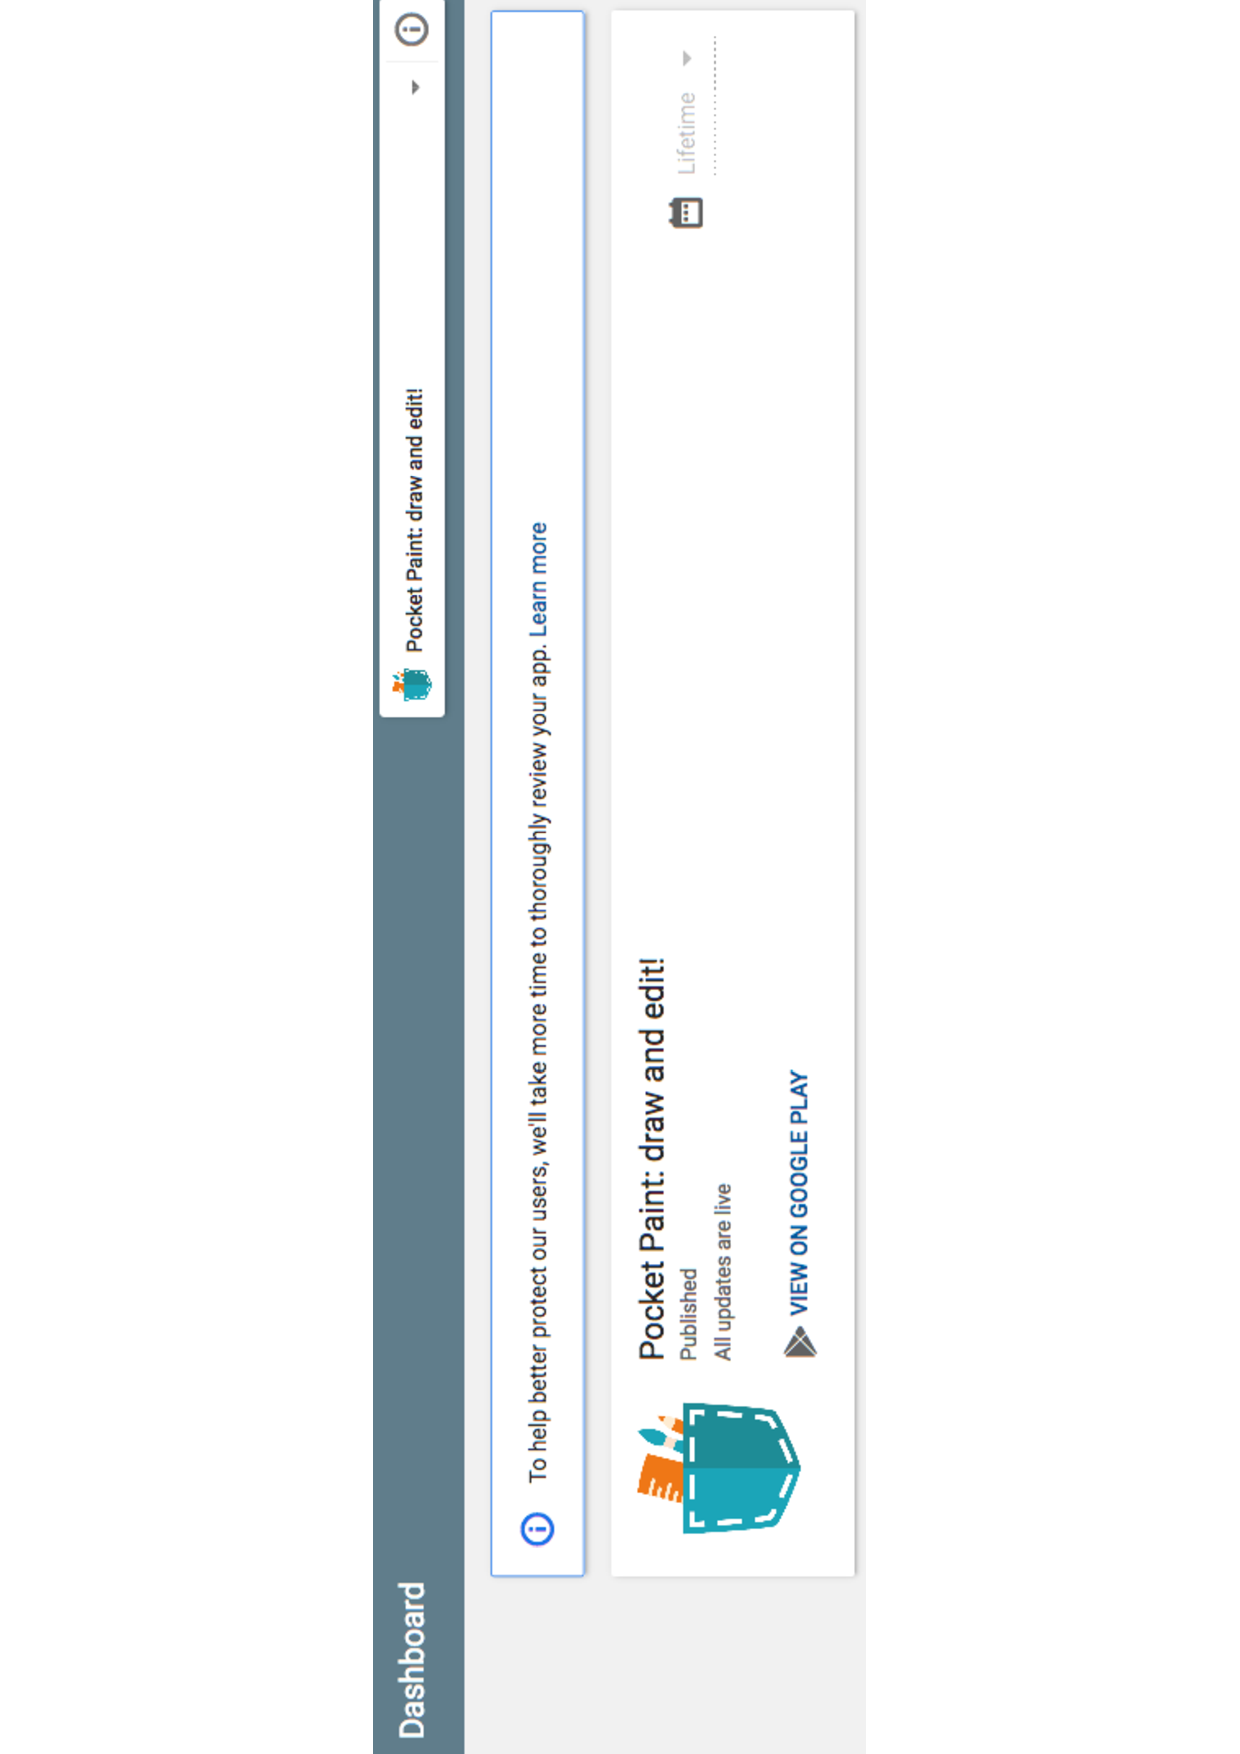
\includegraphics[width=\linewidth]{images/android-vitals-screenshots/catrobat/pocketpaint-to-help-better-protect-users.pdf}
    \caption{Google Play message for Pocket Paint: To help better protect our users...}
    \label{fig:pocketpaint-to-help-better-protect-users}
\end{figure*}

The final view is that of the app store, the `storeholder' in the figure. They have a global and holistic view of the entire store, including \textit{potentially}\sidenote{A caveat on the use of potentially: this is because the app stores are closed systems with limited information about their actual behaviour in the public domain.} all the reviews, user interactions, and whatever usage activities have been performed by all the other three views. 
%\akb{Some explanation of the caveat term 'potential' here would be useful I think - i.e. this is because the app stores are closed systems with limited information about their behaviour in the public domain?}

We now cover various implications of the app store conceptual model.

\subsection{Trust relationships}
One of the key success factors of the modern app store (typified by the Apple App Store and Google Play) was that the platform provider provided the entire ecosystem and established the rules of engagement. The locus of trust is the provider of the app store, which acts as the public face and to some extent also acts as a representative for both the users and the developers. In terms of financial transactions it also acts as the intermediary and facilitates users being able to obtain refunds for app and in-app purchases subject to various conditions. 

Note: There are many details related to the trust relationships for those interested in that topic, however in the interests of focus and concision they are outside the scope of this thesis. 

\subsection{Communications paths and data flows}
There are numerous communication paths for mobile apps both with and without an app store being involved. As the vast majority of apps and users use devices and apps that are part of an app store ecosystem (even if they are obtained from other sources, e.g. as often occurs in India) I will only consider the ecosystem that includes an app store in this thesis. Figure~\ref{fig:sources-of-info-with-app-store-background-ch} illustrates various sources of information for apps available in an app store. The sources and communications paths will be considered next. 
% SHOULD-DO Perhaps a Venn diagram would also complement this illustration?

\begin{figure*}
    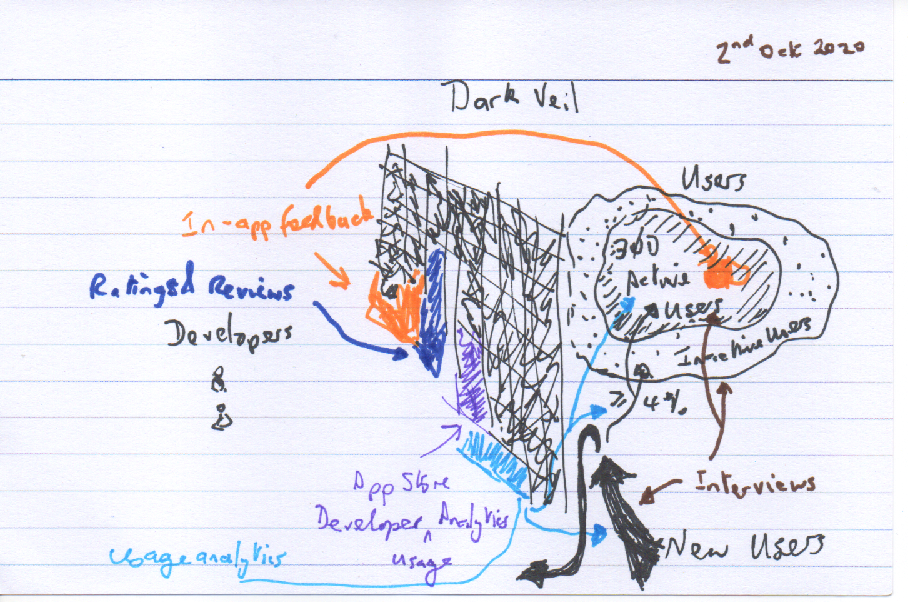
\includegraphics[width=\linewidth]{images/rough-sketches/sources-of-information-with-app-store-1.pdf}
    \caption{Sources of information with an App Store}
    \label{fig:sources-of-info-with-app-store-background-ch}
\end{figure*}

The information about mobile apps can come from users directly or indirectly, from the app if it collects information either directly or indirectly, from devices. Such data collection could be via the operating system, installed apps with privileges to access information about other apps, from accessibility services, and potentially other means e.g. installed viruses. Alternatively, it could come from intermediaries - particularly the app store, and also from network traffic, observers,~\emph{etc.} 

Source code and source code repositories are also useful sources of information about mobile apps. Information can be usefully combined from several sources, for instance from source code about calls to write log messages compared to actual logs recorded when the app has been used on a device. Given the app store plays a pivotal role let's consider its role in terms of communication paths now. 

An app store is more than the store front, it controls and affects many aspects of the ecosystem that gathers around it. It is also more than the software, data and information that the various memberships can access. For instance the modern app stores often include software that is mandatory and pre-installed on end-user devices where that software cannot be easily removed or disabled by users\sidenote{competent, technically savvy individuals may be able to thwart protection mechanisms as may other specialist organisations and software.} . This software includes a local storefront that offers end-users new apps, updates, and enables users to manage optional apps\sidenote{Optional apps can be installed and uninstalled by end users at will. Non-optional apps are installed by various organisations, including the app store provider, some device manufacturers, and so on.}.

The app store provides various primary communications paths between the various parties involved in the ecosystem. It may be an active party, for instance in some of the reports provided to developers and/or users, and in policy-related matters; or it manages communications between app users and developers. Often the app store's owners define the rules of communications, including details such as whether and when apps can ask users to rate an app.

\begin{figure*}
    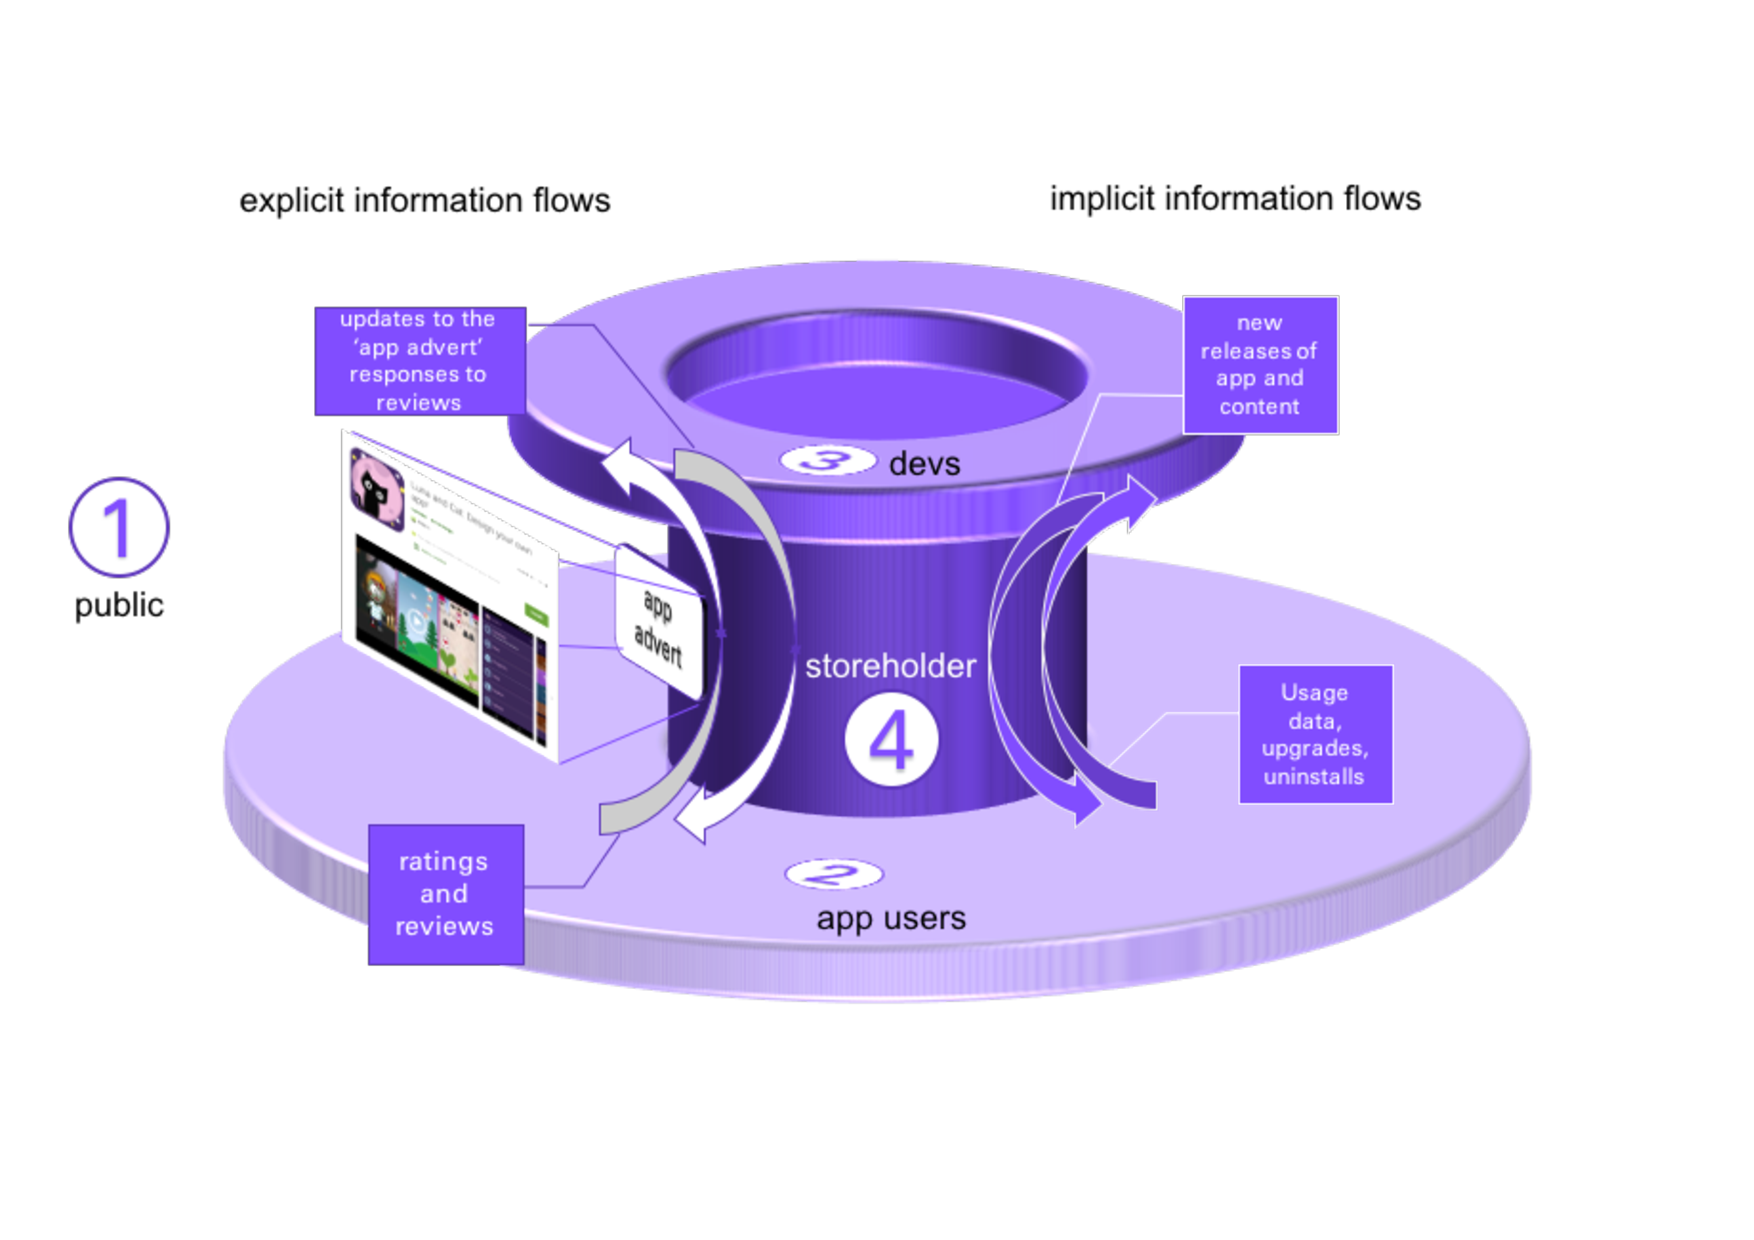
\includegraphics[width=\linewidth]{images/my/app-store-data-flows-3d.pdf}
    \caption{App Store: Communications Paths and Data Flows}
    \label{fig:app-store-data-flows}
\end{figure*}

Some of the communications involves humans, or software chatbots masquerading as pseudo-humans intended to behave similarly to how humans would do in similar circumstances, for instance to provide in-app assistance~\sidecite{baez2021_chatbot_integrations} and to help developers respond automatically to app reviews~\sidecite{greenheld2018_automating_developers_responses_to_app_reviews}. Other communications is generated by software, for instance usage and diagnostic data collected by the operating system and related utilities on a mobile device (collectively described as the platform).

%\akb{Why are bots characterised as 'pseudo-humans'?}

The communications paths and data flows in an app store ecosystem are illustrated in Figure~\ref{fig:app-store-data-flows}. There are two forms of data flows: explicit and implicit. Explicit data flows are actively and intentionally performed by one or more of the participants, implicit data flows represents information that can be inferred or gleaned from various actions and inactions.

Examples of actions intended to communicate explicitly include:
\begin{itemize}
    \item Making the app available in the app store; this includes creating screenshots, a description of the app, adding meta data the app store requires and/or requests, \emph{etc.} This information becomes public if the app store approves the app for release.
    \item Ratings and reviews performed by app users. Only a subset of users provide these, the percentage varies from zero to a maximum of around 10\% with typical percentages around 1\% to 3\%. % SHOULD-DO find credible source for these estimates, I've checked various sources without success
    Estimates vary, partly as the definitions vary too. AppBrain states 46.5\% of Android apps do not have a rating~\sidenote{Their definition is \emph{``Apps that have less than 3 ratings we consider to not have a rating yet"}~\url{https://www.appbrain.com/stats/android-app-ratings}}. In comparison, 42matters.com estimate 41\% of Android apps and 57\% of iOS apps have no rating~\sidenote{\url{https://42matters.com/stats}}.
    \item Responses to reviews, for example Google Play allows developers to respond to reviews, and for both reviewers and developers to update their reviews and responses.
    \item Suspending an app so it is no longer available to users to download. Storeholders sometimes suspend apps and even developer accounts where they perceive the app and possibly the developer contravenes the app store's policy. % c.f. the recent ban of Fortnite in both Apple and Google stores. And see the comment after this article re German law https://www.overpass.co.uk/google-play-account-suspended/ 
    %\href{https://www.ape-apps.com/viewpage.php?p=34186}{My Colony Suspended from Google Play}
    %\href{https://www.ape-apps.com/viewpage.php?p=34173}{My Colony removed from Google Playstore} - over 50% of users come from Google Play.
    
\end{itemize}
%%%%%%% Various interesting sources of Android- (and some iOS) related stats
% https://www.businessofapps.com/data/app-statistics/
% https://www.statista.com/statistics/266217/customer-ratings-of-android-applications/ (seems to be a rehash of AppBrain's report)
% https://mindsea.com/app-stats/
% 

%\akb{Use consistent labels for concepts - below you refer to '(implicit) information flows' whereas above you use '(explicit) actions intended to communicate'.  By using different labels you are suggesting that these two implicit/explicit categories are not directly comparable, i.e., they are different types of things altogether. However, I am not sure this is your intent.}

Implicit information flows include:
\begin{itemize}
    \item New releases of apps and related content (such as in-app content, often purchased using in-app purchasing). These indicate the developer is wishes to actively engage their userbase. Upgrades may include changes to the app seeded by various sources such as ratings and reviews and other data, including:
    \item Usage data and upgrades, both imply the software provides some value to the users. Lack of usage may also be an indication the software is not currently providing value - this may be expected for instance with seasonal apps. Uninstalls are a stronger signal that users no longer see sufficient value in the app to keep it on their device.
\end{itemize}

On-device bug reports may be a hybrid, where the bug reporting utility on the device does much of the data collection and may report this automatically and transparently, however it may sometimes ask the user for additional input and permission to send the bug report.

\subsection{Membership criteria of each group}
%\akb{Explain why the membership criteria are important to understand, perhaps combine with next section single explanation of groups and what members can do in each}
As Figure~\ref{fig:app-store-data-flows} illustrates there are four numbered groups in the illustration. People can potentially belong to more than one group (albeit membership of the storeholders is limited to owners and those they assign membership to,~\emph{e.g.} as administrators of the app store). Group membership constrains what the members can do as participants and what they have access to.

\begin{enumerate}
    \item Public: the membership criteria are minimal. Here `public' is any entity, human or technological, that has access to the app store\sidenote{For our purposes we can assume online digital access, other modes may also be viable, for instance some researchers use archives of data sourced from app stores.}. An example of a technological entity, is a search engine crawler or software including web scraper technology and scripts that use APIs provided to obtain information about apps in the app store.
    %\akb{Not sure what is meant by 'minimal' here. You could describe 'public' as any entity, human or technological, that has access to the app store. Provide an example of a technological entity, e.g., a search engine crawler}
    \item App user: the public can use an existing account or create a new account with the app store that would allow them to become an app user~\sidenote{They need to meet the criteria of the app store.}. Note: there may be restrictions or constraints that mean not everyone can install every app on every device, however the general practice is that apps are freely available for app store users to install on any device they possess. 
    \item Developer: developers need to be registered and validated by the app store, the process varies for specific app stores, they often involve payment of a fee and some amount of validating their identity. Some app stores may perform additional checks based on information they and/or others hold.  
    \item Storeholder: they are generally a legal entity, and certainly for the purposes of this research they are. Apart from a few exceptions (such as F-Droid~\sidenote{Details are available online at~\url{https://www.f-droid.org/en/about/}}) they are multi-national major corporations.
\end{enumerate}


\subsection{What participants can and cannot do (and who dictates the rules?)}
%\akb{You don't explain the link between the implicit/explicit data flows and these membership groups.}
\begin{itemize}
    \item Public: The public cannot review an app or easily download the app. They can view publicly accessible information, including information that was gathered previously, potentially by others.
    \item App user: They can rate and review apps they have installed on their account~\sidenote{ user may have several devices and choose not to install an app on all of them. Also some apps may by limited to devices that meet particular criteria e.g. the platform version.} or device. They can also install, update and deinstall apps~\sidenote{There may be restrictions imposed for some apps, for instance Google Apps and Manufacturer apps might be blocked from being uninstalled, and updates are sometimes mandatory, \emph{etc.}}.
    \item Developer:  Approved developers can upload apps to the app store and publish them if the app store also approves the release. They can choose to submit new versions of their apps, sometimes they may be required to do so by the app store. They can choose to suspend or withdraw their app from the store, note: generally users can continue to use the app if they have it installed. Developers are expected to interact with the app store and often do so of their own volition, for instance to see how their app is `doing'. The developer may define a price for their app and/or any in-app purchases. They may also require users comply with additional terms of use, and many apps do so.
    \item Storeholder: They are by far the most powerful participant as they establish the ecosystem including the rules of engagement and enforce these rules. The app store has the right of delay or veto of releases, it can suspend apps and developers, and much else besides. They are expected to comply with the laws of the various countries the app store is available in and also where their business is situated. These laws may affect the developers and the app users, for instance the amount of sales tax charged on a purchase in the app store.
\end{itemize}

We have already identified four membership groups involved in app store ecosystems, there is at least one more and also additional data flows in the ecosystem. The fifth membership group is a~\emph{service provider}. These service providers provide non-trivial functionality and other capabilities such as in-app analytics, feedback, and so on. Developers can choose to incorporate software libraries into their apps and use the services provided, for instance as conduits of communications between the app and the developers. Here developers include other specialist groups in their organisation such as customer service personnel and marketing teams. Many app developers choose to use at least one such service, some incorporate several and there is even specialist software that enables developers to manage multiple similar services within their apps on end-user devices. An example of this type of software is~\url{https://github.com/segmentio/analytics-android} (other platforms are also supported and there are other providers of similar software).

Membership matters in particular because of who has access to which data and for how long they have access. Note: Control and `ownership' of the data are also relevant topics, however they are not necessary to comprehend the rest of this topic. % SHOULD-DO consider whether to add material on this topic in the thesis. 

\subsection{Phases of a release}


\begin{figure*}
    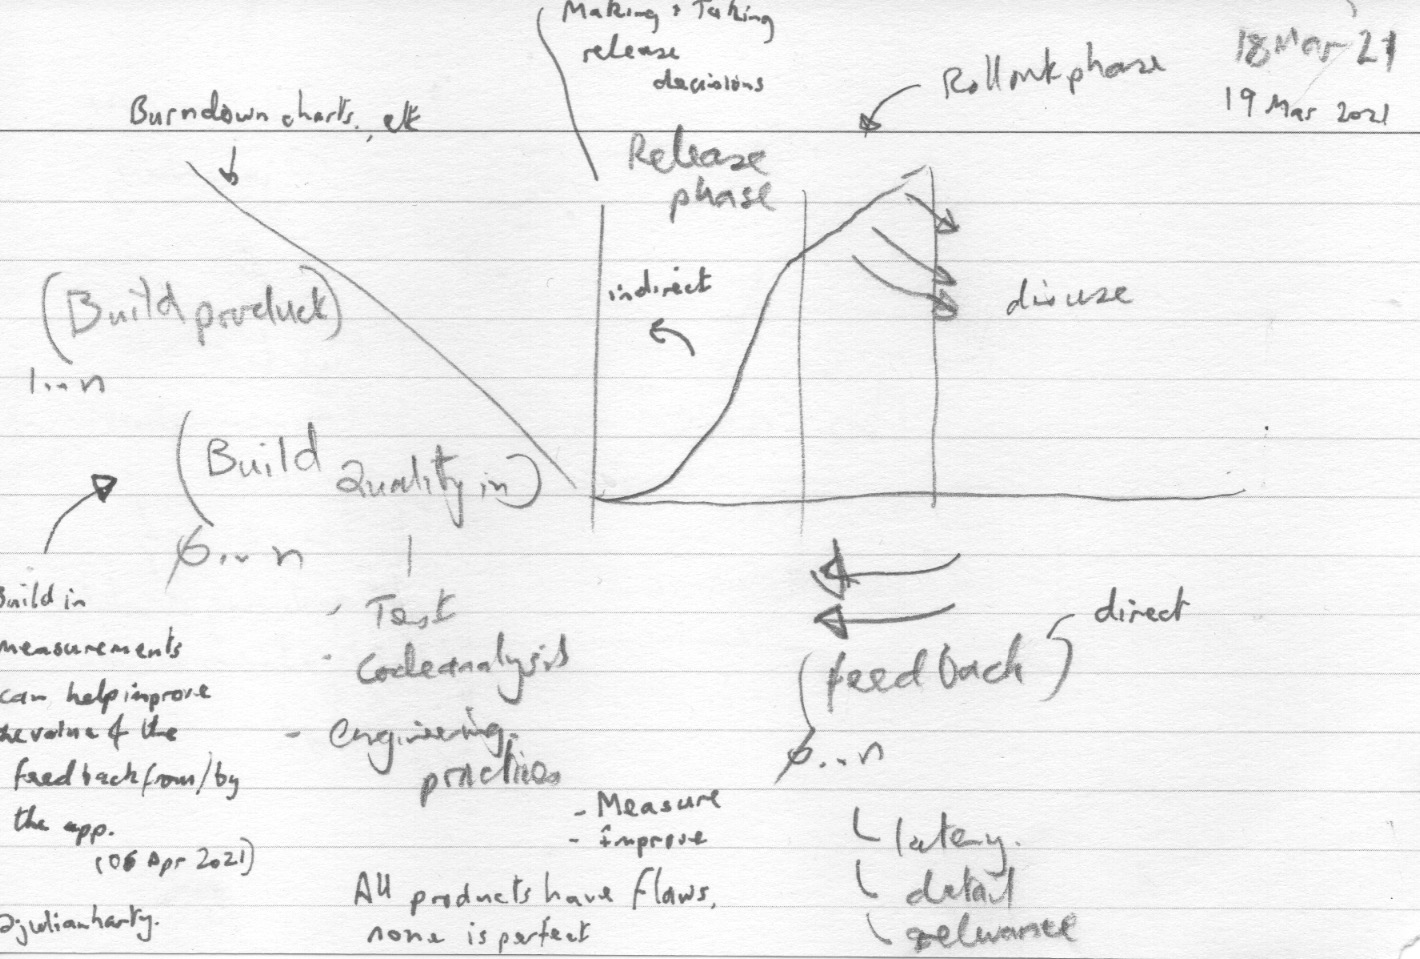
\includegraphics[width=\linewidth]{images/rough-sketches/Red-Thread-Rough-Sketch.jpeg}
    \caption{The lifecycle of a release and where mobile analytics provides feedback}
    \label{fig:red-thread-for-this-thesis}
\end{figure*}

For any given release of a mobile app there are at least three material phases in order for the release to be used:
\begin{enumerate}
    \item Building the product: which may incorporate practices and tools intended to ship a `quality product'. Some teams also incorporate logging and reporting to help measure the behaviours of the app in use, post release.
    \item The Release: For some projects this may be as simple as uploading a new binary and making it fully available. For others they may incorporate decisions and mechanisms to make each release with the aim of de-risking any undesirable/adverse effects of the new release.
    \item Deployment: Deployment occurs when end users install and start using the release of the app. Both the app store and the end users affect when this occurs. App developers can try to hasten when users install the latest release through various mechanisms, for instance through implementing and mandating users upgrade their current release.
\end{enumerate}

Figure~\ref{fig:red-thread-for-this-thesis} illustrates these three phases together with some of the dynamics \emph{e.g.} of rollout and disuse of a release, and of feedback from whatever sources that the development teams can choose to pay attention to and apply. These phases are part of a longer lifespan of the release that includes an often long-term postdelivery period~\sidecite[][pp 156-157]{evans2004_achieving_software_quality_through_teamwork} where users use the release until it is decommissioned or replaced with a subsequent release.

\begin{figure*}
    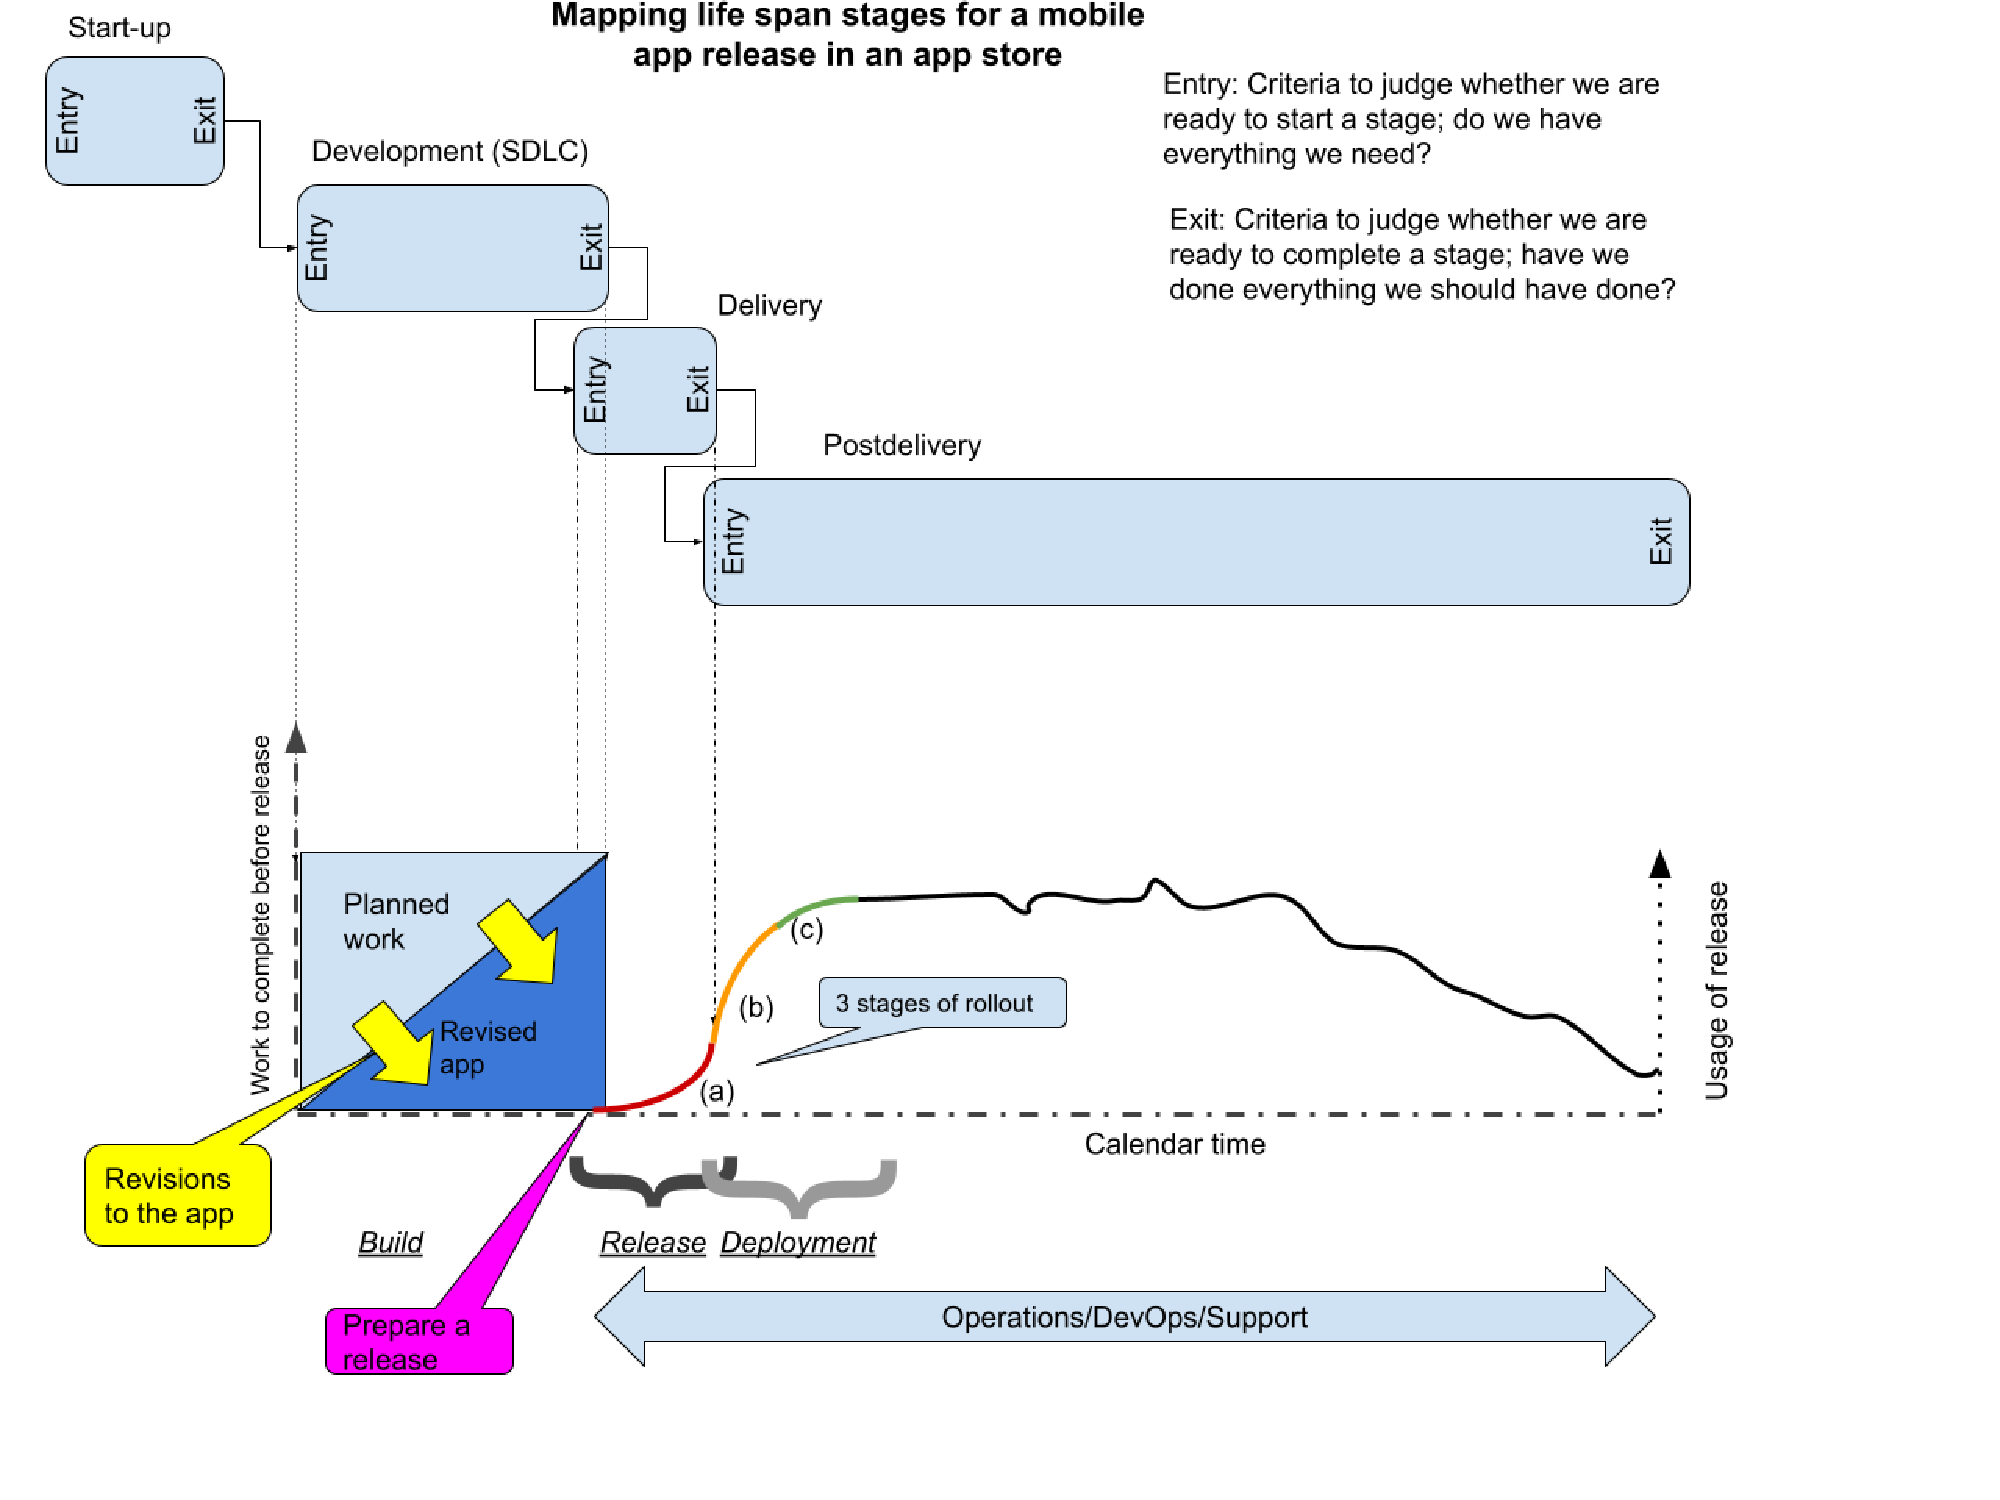
\includegraphics[width=\linewidth]{images/my/mobile-app-life-span-stages-21-sep-2021.pdf}
    \caption{Mapping life span stages for a mobile app release in an app store}
    \label{fig:mobile-app-life-span-stages}
\end{figure*}

Figure~\ref{fig:mobile-app-life-span-stages}~\sidenote{Source of figure, Google Drive file: \href{https://docs.google.com/document/d/1d4B5l1tlpclHdKwY8W00qchiCV2YK5JjJP8TbkRHcjQ/edit}{Mobile app life span stages}.} compares a revised version of the `Life span stages' Figure in~\sidecite[][p.155]{evans2004_achieving_software_quality_through_teamwork} mapped approximately to the three stages first illustrated in Figure~\ref{fig:red-thread-for-this-thesis}. Mobile app releases in an app store extend the Delivery which may also overlap either or both the development and the postdelivery life span stages. The overlap with the development stage is because the development is not complete until the app store accepts/approves the release (this may include pre-launch checks, automated testing, and so on depending on the app store). The overlap with deployment happens as releases are often released incrementally initially to a small percentage of the userbase - at least some of the users in that percentage will install the new release, until the percentage has been achieved. Meanwhile at least some of those users will use the app which will then mean the release is operational and may need operational support.


\section{Conceptual model of layers within apps and observation points}
Observation can be internal,~\emph{i.e.} built into apps, and external. External includes instrumentation, debugging tools, the operating system at runtime, accessibility interfaces, event listeners, log watchers, and so on (as this is not intended to be an exhaustive list). The observation may also be indirect, for instance using network monitoring software, and/or from remote APIs, REST endpoints, and web servers (with their attendant logging).

\subsection{Three layers of an app}
In earlier work, published in ~\sidecite{harty_aymer_playbook_2016}, the concept of three layers of an app was introduced. These are illustrated in Figure \ref{fig:3-layers} and shows three primary conceptual layers related to a mobile app. 


\begin{figure*}
    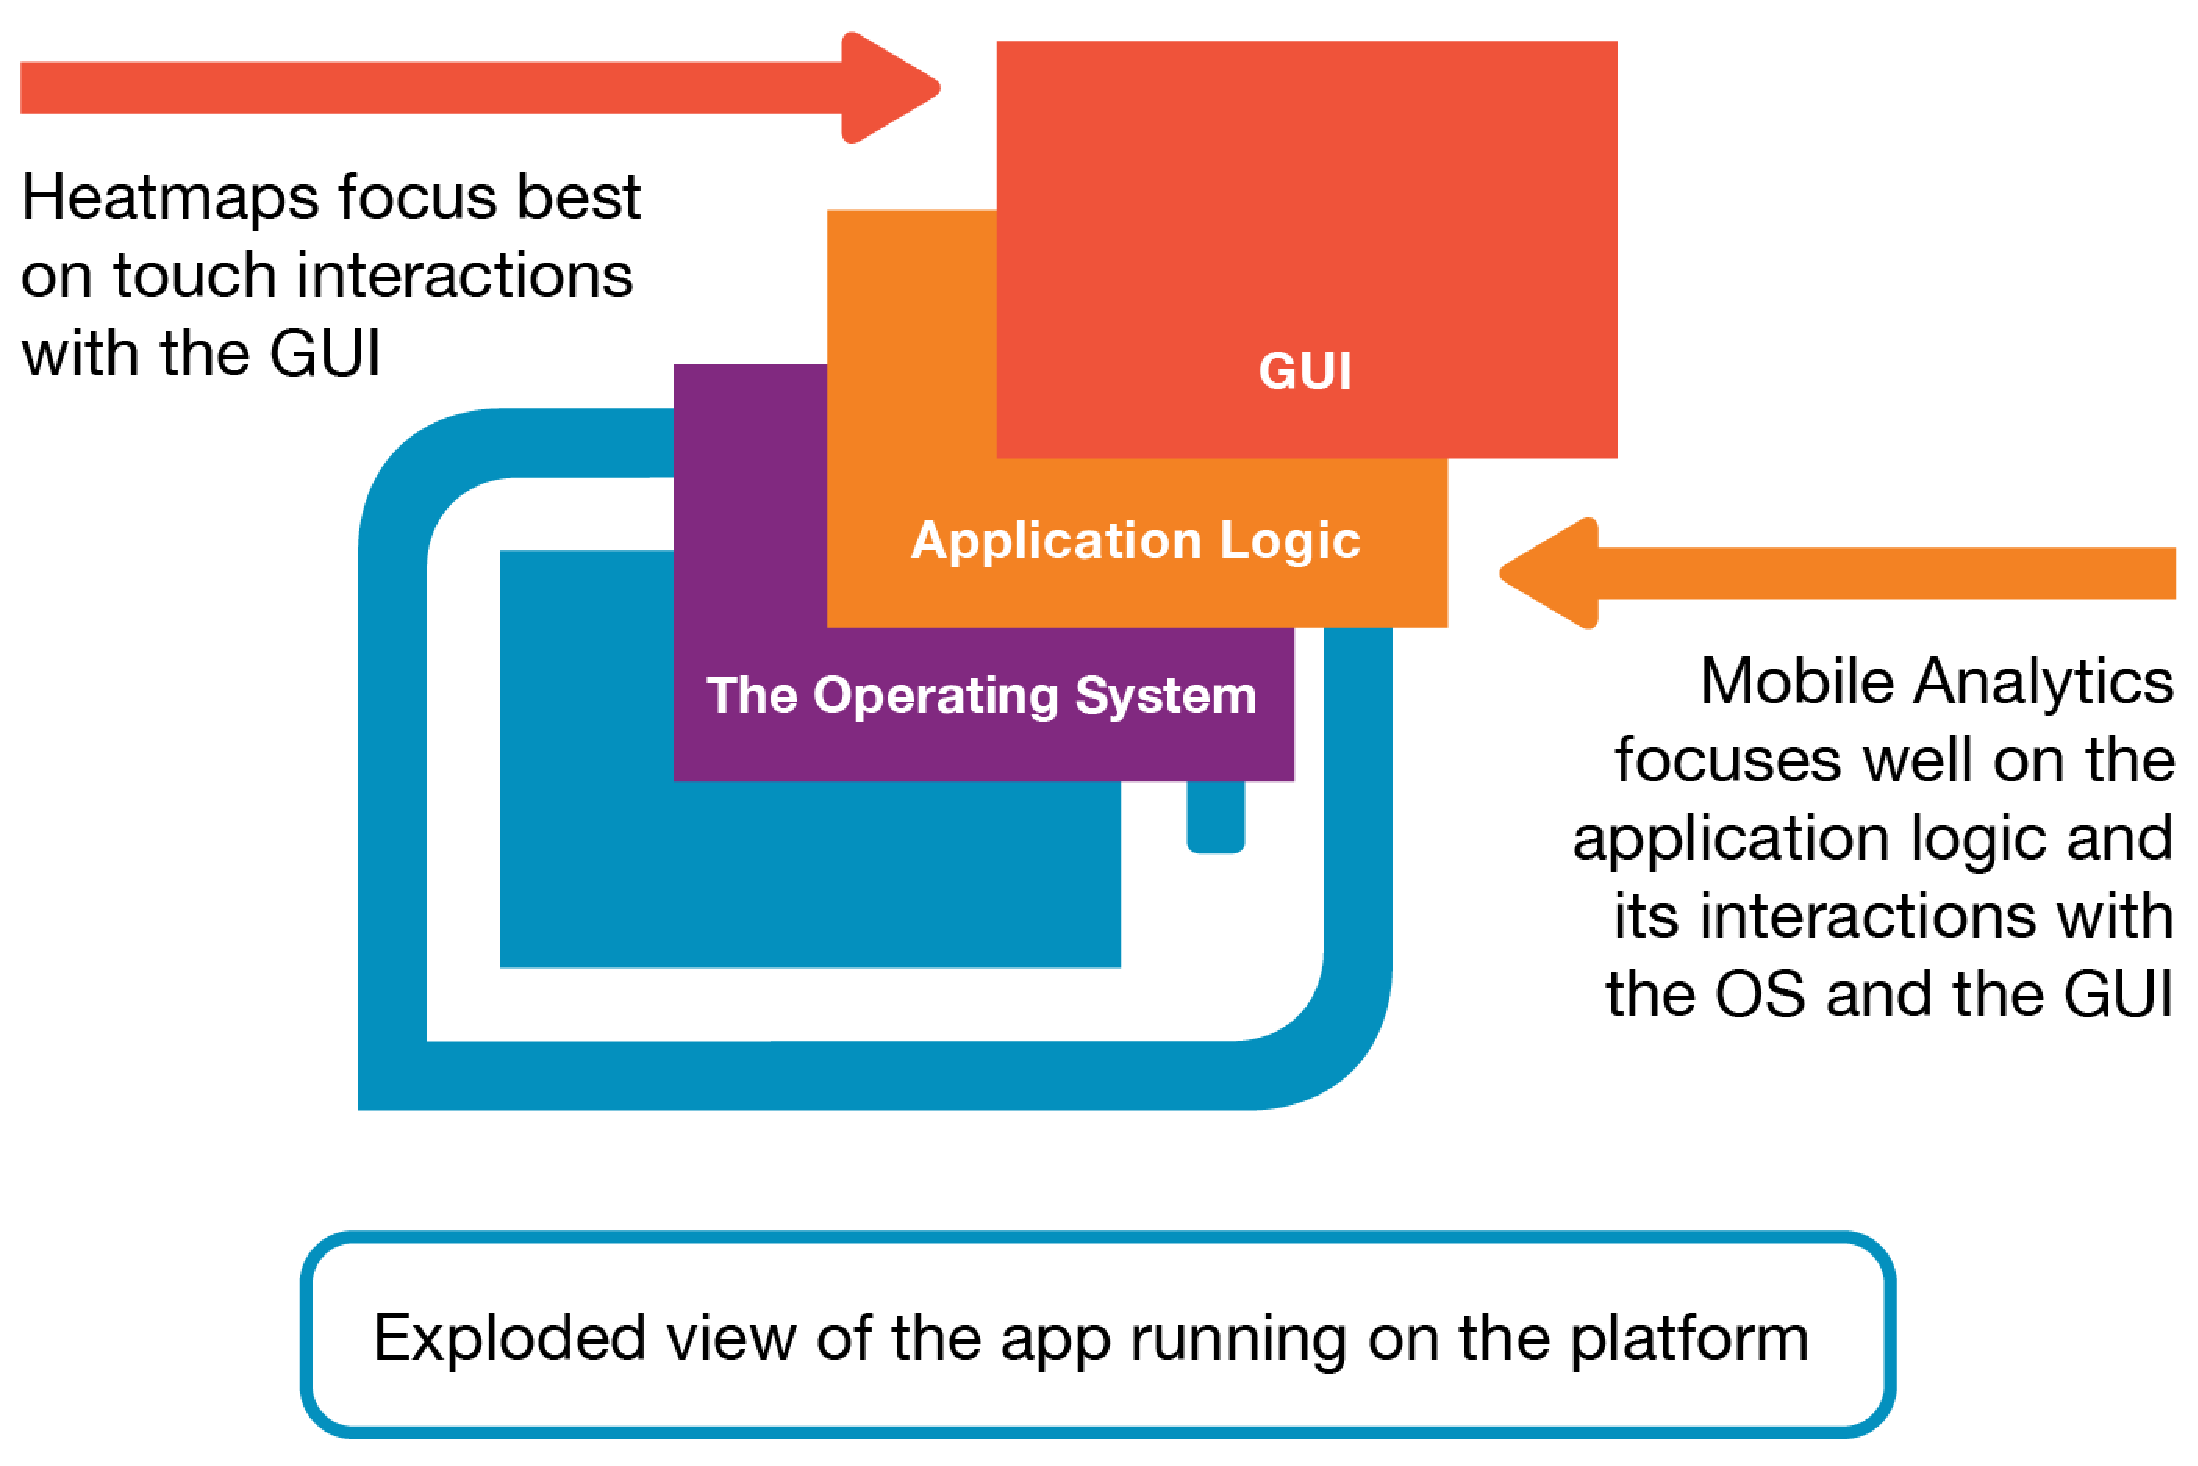
\includegraphics[width=\linewidth]{images/mobile-analytics-playbook/3-layers.pdf}
    \caption[Three layers of an app]{Three layers of an app {Image credit: First published in The Mobile Analytics Playbook~\cite{harty_aymer_playbook_2016}}.}
    \label{fig:3-layers}
\end{figure*}

Of course, apps aren't quite this simple or well defined in reality, for instance they include software libraries from various sources, A/B testing utilities, logging code, run-time lifecycle management, and so on. Nonetheless, these three layers are a useful abstract, particularly in terms of useful observation points about apps on user's computer devices~\sidenote{Another observation point that was orthogonal to the application logic layer was one popularised by a company that has since been acquired, called SafeDK. They provided app developers with software that provided an interface between the developer's code and the libraries the code used. This software collected and reported usage data on the performance and reliability of the libraries. Given the commercial nature of the business, their acquisition and the demise of their products and the company's website, and the fast moving nature of the internet, obtaining concrete information may be impractical for all but a few people who know those who were involved at the time.}.

The \Gls{gui} can be visually observed by sighted users, it can also be observed by Accessibility software, and test automation tools, \emph{etc.} externally to the app. It can also be observed from within the app, for instance through using software known as \emph{heatmapping} that records the screens and the touch interactions performed by users of that screen. One of the the more popular, mature heatmapping offerings is from AppSee~\sidenote{\href{  https://www.appbrain.com/stats/libraries/details/appsee/appsee}{AppBrain stats for AppSee}. Note: in 2019 Appsee's team was ~\href{https://techcrunch.com/2019/05/13/servicenow-acquihires-mobile-analytics-startup-appsee/}{acqui-hired by ServiceNow} and the service no longer directly available.}, nonetheless they are only used in a small minority of mobile apps.


\subsection{Observation points: inside-outside perspectives}
The observation point determines what can be observed and how. 
As Figure~\ref{fig:internal-external-table} illustrates there are internal and external perspectives on an app for various purposes, including observations, interactions (e.g. through test automation), and emitting information (e.g. through logging, reporting, or mobile analytics). Where the information is observed affects what can be known and what is possible, an insider is privy to information an outsider is not; whereas an outsider has perspective and can potentially perceive things insiders cannot.


\begin{figure*}
    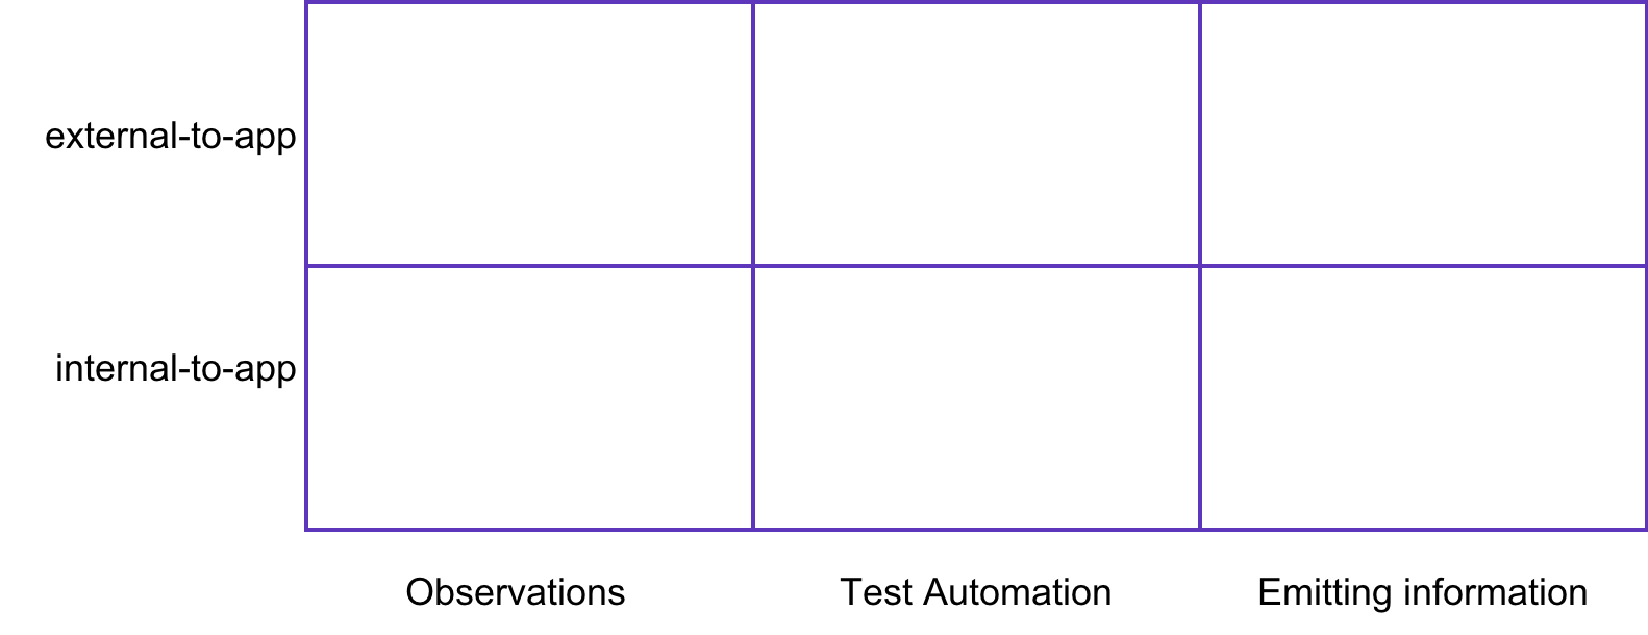
\includegraphics[width=\linewidth]{images/internal-external-table.pdf}
    \caption{Internal and external perspectives of an app}
    \label{fig:internal-external-table}
\end{figure*}

%\textbf{SHOULD-DO} Expand the following: What is test automation? discuss how mobile apps are tested, the unique aspects of using accessibility interfaces, etc.


\section{Conceptual model of analogue and digital feedback}~\label{analogue-and-digital-feedback}
Feedback can help developers to find and choose ways to improve their software. Various researchers have investigated way to understand and use feedback provided by end-users, for instance, in ratings and reviews users provide to the app store. For the purposes of this research feedback people provides is considered~\emph{analogue feedback} as it has the richness and complexity of analogue signals, and also challenges of processing and comprehension.

In contrast, digital feedback originates from software and is generally deterministic~\sidenote{~\url{https://en.wiktionary.org/wiki/deterministic}}. For the purposes of this research~\emph{digital feedback} is provided by running software where programmers added code to programs to collect data that provides feedback about software use and certain behaviours of that software. The addition of the code may be automated, in part, or wholly, for instance by another program or script. As an example, AppPulse Mobile claims they can add analytics automatically without developers writing a line of code~\sidenote{~\url{https://www.microfocus.com/en-us/products/apppulse-mobile-app-apm-monitoring/overview}}.

\begin{figure*}
    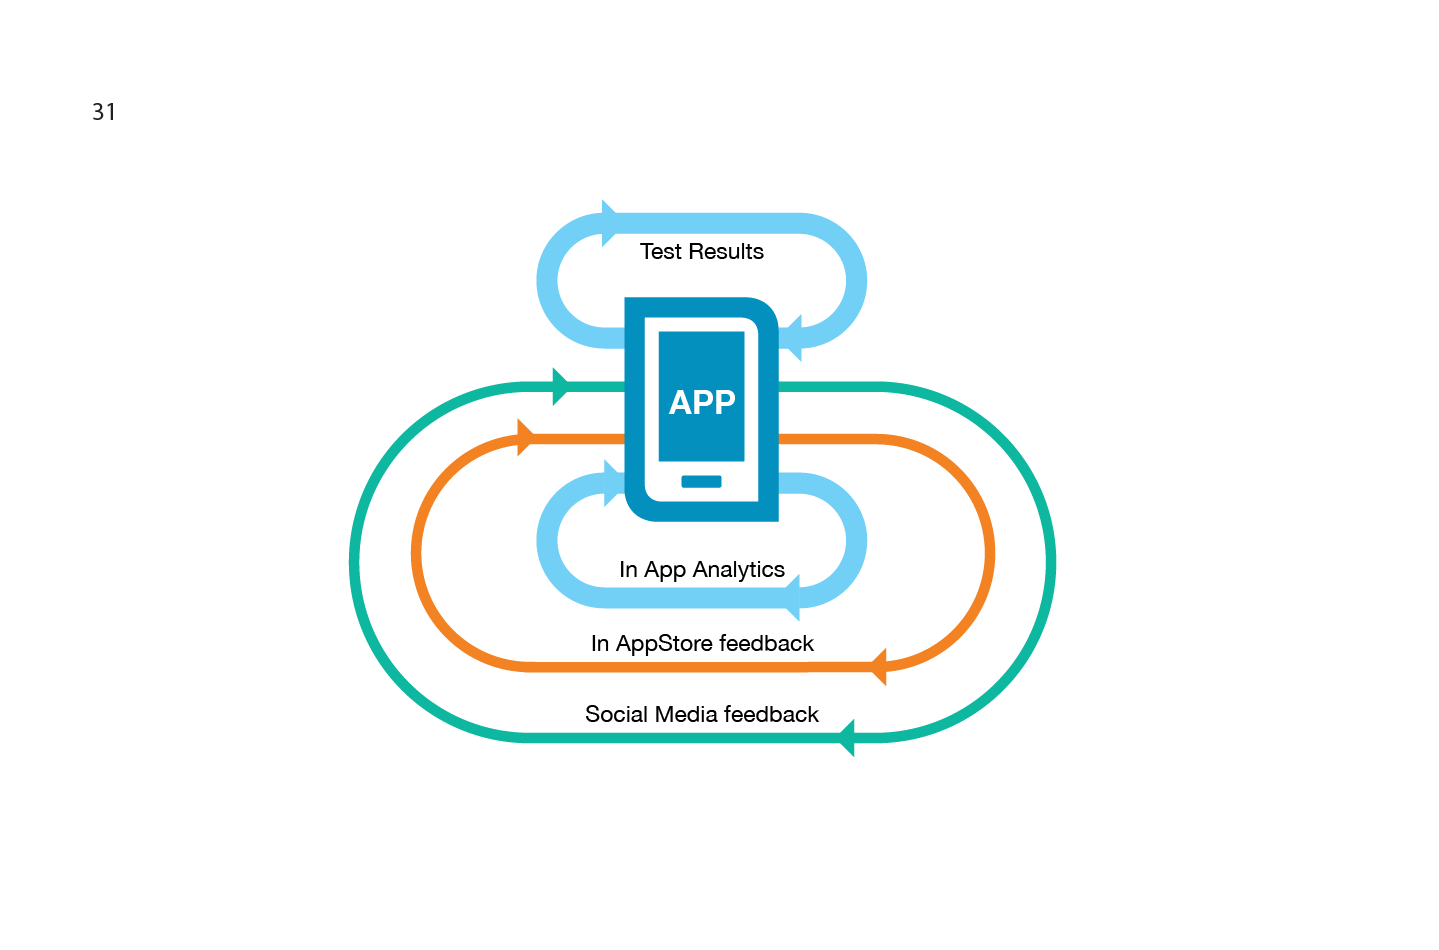
\includegraphics[width=\linewidth]{images/mobile-analytics-playbook/Chart-07-FeedbackLoops.pdf}
    \caption{Feedback Loops for mobile apps~\cite{harty_aymer_playbook_2016}}
    \label{fig:map2015-feedback-loops-for-mobile-apps}
\end{figure*}
%SHOULD-DO edit the figure to remove whitespace, etc.

Figure~\ref{fig:map2015-feedback-loops-for-mobile-apps} illustrates various feedback loops where the feedback could be used to change and improve a mobile app. Within the team's aegis are test results (and static analysis, etc.). Beyond their direct control are feedback within the app, within the app store, and outside the app store ecosystem such as feedback on social media about their app. This figure illustrates in-app analytics which was the primary form of analytics at the time the figure was published, since then two additional forms of feedback have emerged: platform-level feedback such as Android Vitals and in-app feedback.

\subsection{Analogue feedback: in-app tools}
One source of feedback is when apps include feedback mechanisms within the app. Various benefits are touted to encourage developers to add such feedback including the ability to: ~\emph{``...capture valuable insights into the usability of the app and quickly resolve any issues..."}~\sidecite{mopinion2017_top11_mobile_in_app_feedback_tools}, for example. 

Some apps also collect in-app feedback if the user indicates they are not satisfied with the app and conversely ask users to submit a review online in the app store if they are satisfied. One hypothesis is their developers have implemented this approach to divert adverse ratings and reviews from public view and from the app store algorithms. 

In-app feedback enables a wider range of communications and also scope for richer dialogues than relying on feedback mechanisms provided by app stores which consist of a rating and an optional plain text comment. Examples of wider ranges of communications include surveys, and richer dialogues include audio recordings.

In-app feedback has also been proposed for bi-directional communications between developers and users of the app for instance to elicit non-functional requirements~\sidecite{avellis_harty_yu_towards_mobile_twin_peaks}.

\subsection{Analogue feedback: app store feedback}
App store feedback, combines a rating (typically using a one- to five- start rating and an optional plain-text comment). It is a subject covered by significant volumes of research and discussed in the related works chapter. %MUST-DO actually write up this related research and contrast it with mobile analytics.

\begin{figure*} %[!htbp]
    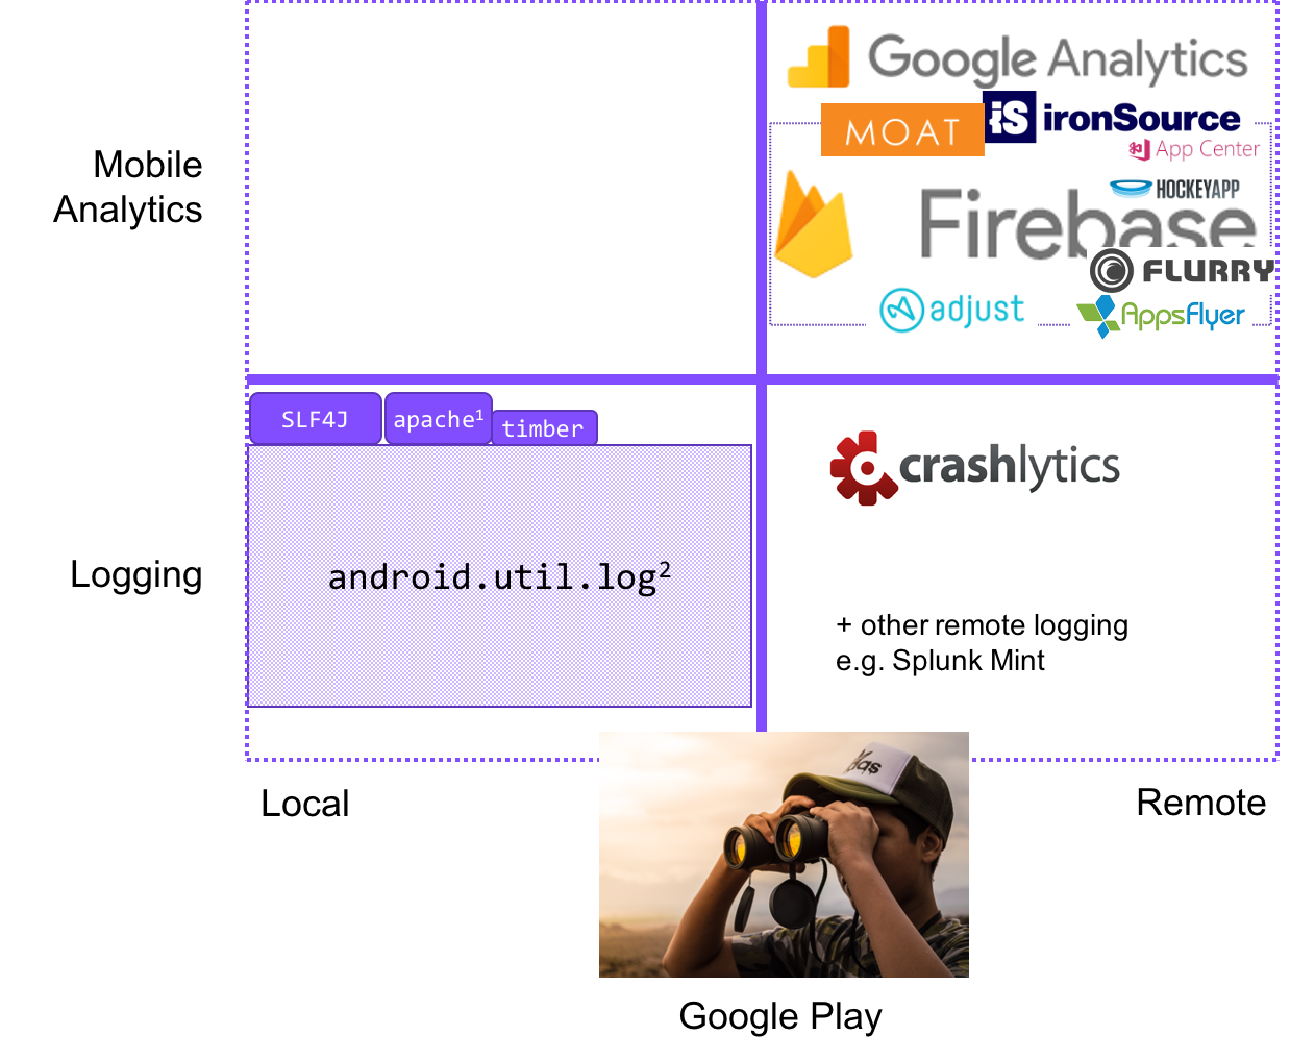
\includegraphics[width=\linewidth]{images/matrix-of-logging.pdf}
    \caption{Matrix of logging}
    \label{fig:matrix-of-logging}
\end{figure*}

\subsection{Digital feedback: logging and mobile analytics}
The application may incorporate logging and/or mobile analytics. Logging in mobile apps is often used locally, by developers independently of other mechanisms. Mobile analytics is used remotely, as are crash reporting libraries. 



Figure \ref{fig:matrix-of-logging} illustrates a matrix of logging, where logging and mobile analytics are on the Y axis and local and remote on the X axis. There is a cross-cutting example where the mobile platform observes local events and then forwards the information remotely. A good example is Google Play which appears to be an external observer of data recorded in device logs. Data collection runs locally and is sent to Google servers where Google analyses the data and provides reports to developers for their apps. %SHOULD-DO check for related US patent filings by Google in this area.

\begin{table} %[!htbp]
    \centering
    \begin{tabular}{lll}
         Category of logging &Local access?  &Remote access? \\
         \hline
         None            &N/A  &N/A \\
         \texttt{StdOut} &It depends &Unlikely \\
         Default platform logging library &Yes &Possible \\
         Enhanced platform logging library &Yes &Possible \\
         Third-party logging library &as-designed &as-designed \\
         Proprietary logging library &as-designed &as-designed \\
         
    \end{tabular}
    \caption{Choices available to developers for logging in mobile apps}
    \label{tab:logging-choices-for-devs}
\end{table}

Table~\ref{tab:logging-choices-for-devs} identifies various categories of logging available to developers of mobile apps. They range from no active logging in the app (some information is still logged by the platform) to proprietary custom logging libraries which a tiny minority of development teams would chose to do - they may do so to keep their logging as private as practical from the rest of the device.

\texttt{StdOut} is often used in code written for other platforms including Linux that has been ported to mobile platforms. Some people who are unfamiliar with logging libraries who have a superficial understanding of developing for mobile devices may also use print statements in their code (which effectively writes to the standard output) rather than use log statements in their code. There are various nuances of how the standard output and standard error outputs are handled in Android code (Java, Kotlin, etc.) and native code (C/C++) are directed as standard for Android apps. In short, for native code (\emph{e.g.} written in C/C++) as standard the outputs are discarded by `writing' them to~\texttt{/dev/null}. For Android code (\emph{e.g.} written in Java/Kotlin) \texttt{System.out} and \texttt{System.err} can be redirected to the log on some Android releases if the device is configured to do so.
%MUST-DO add references for https://github.com/android/ndk/issues/671 and https://codelab.wordpress.com/2014/11/03/how-to-use-standard-output-streams-for-logging-in-android-apps/ and https://stackoverflow.com/a/17199704/340175 and https://stackoverflow.com/questions/10531050/redirect-stdout-to-logcat-in-android-ndk

There are various enhanced log libraries, for instance~\texttt{timber} which are used by discerning app developers. These libraries also write to the platform log files. 

To Be Continued. %MUST-DO

\begin{figure*}
    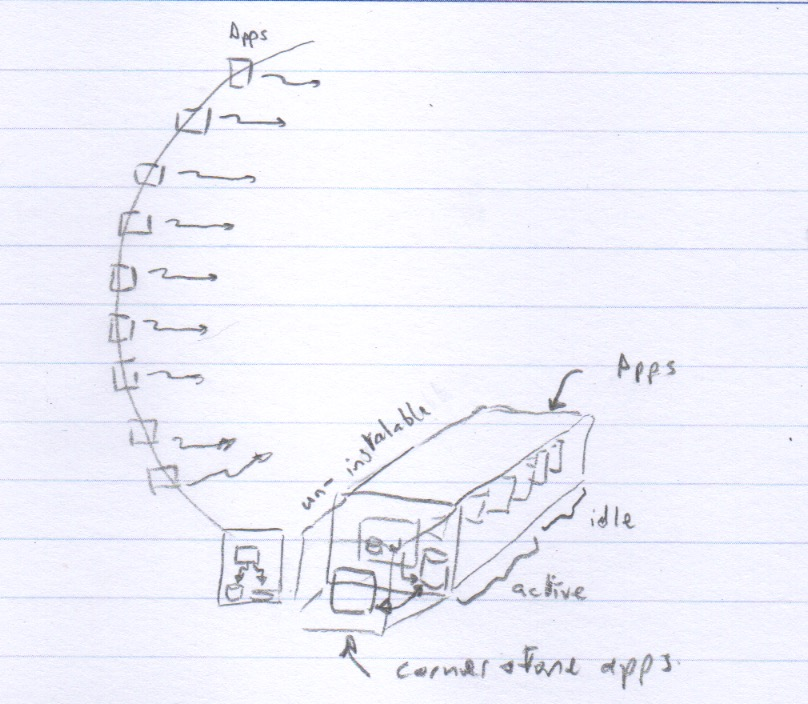
\includegraphics[width=\linewidth]{images/rough-sketches/apps-on-device-boundaries-sketch.jpeg}
    \caption{Apps on the device boundaries}
    \label{fig:apps-on-device-boundaries}
\end{figure*}

\begin{figure*}
    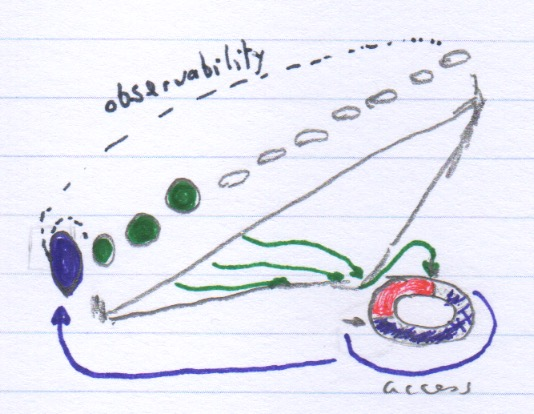
\includegraphics[width=\linewidth]{images/rough-sketches/on-device-logging-sketch.jpeg}
    \caption{On-device logging}
    \label{fig:on-device-logging}
\end{figure*}

A couple of rough sketches, Figures~\ref{fig:apps-on-device-boundaries} and~\ref{fig:on-device-logging} present two views of apps installed on any given mobile device. These apps are broadly one of three categories: platform, pre-installed (non-removable), and user-installed (removable). Here the focus is on their use of logs on the device.

At any point one or more of these apps may be running, the rest are idle. The majority of these apps, with the possible exception of system apps, write to one or more shared, common, log files. These log files have a finite size, and once they are filled newer messages overwrite the oldest ones in turn. In Figure~\ref{fig:on-device-logging} the left-most blob, in purple, represents a system app that is able to read the shared system log files. These apps are pre-installed by the manufacturer, they may include those from the provider of the platform, particularly from Google for Android devices that use Google Play, and also some device manufacturers may have similar apps. Other apps are also pre-installed by manufacturers including a suite of apps from Google and some from the manufacturer. They may also include apps from organisations with agreements with the device manufacturer, for instance they may pre-install some games and utilities from partners. TBC.


As an observation the vast majority of Android developers use the default inbuilt logging library \texttt{android.util.log} and choose one or more of Google's analytics offerings (which include Firebase and Crashlytics). A commercial organisation, AppBrain, provides current statistics for third-party logging libraries~\sidenote{Logging libraries (note the default android log library is not tracked at the time of writing~\url{https://www.appbrain.com/stats/libraries/tag/logging/logging-libraries}}, crash libraries~\sidenote{\url{https://www.appbrain.com/stats/libraries/tag/crash-reporting/android-crash-reporting-libraries}} and mobile analytics~\sidenote{\url{https://www.appbrain.com/stats/libraries/tag/analytics/android-analytics-libraries}}. Some apps have several of these libraries so counts may exceed 100\% in their reports.

\begin{itemize}
    \item Logging: enables developers to understand what their software is doing. The practice is commonplace across many software domains including mobile apps, and each platform and language includes a standard method of generating log messages. These messages tend to be small and intended for immediate, local consumption. On Android when developers use the standard logging library (\texttt{android.util.log}) their log messages are written to a shared circular log file on a device. As illustrated in Figures~\ref{fig:apps-on-device-boundaries} and~\ref{fig:on-device-logging}, some privileged Android software is able to read these shared logs. Developers can also read them using standard Android development tools \emph{e.g.} \texttt{adb logcat} providing they are connected to the device with the log file. Older versions of Android allowed apps to read the full contents, more recently apps are restricted to only the log messages they wrote unless they are granted the relevant permission by Google and the user. 
    In other domains \emph{e.g.} web servers, infrastructure software, and many others, logging is used for production monitoring, fault-finding and analysis. A minority of mobile app developers use remote logging.
    \item Mobile analytics, can extend and scale logging. For mobile analytics, a minority of developers incorporate custom implementations, however the vast majority who use analytics do so through using third-party analytics libraries such as Google Firebase Analytics, details of the current usage of analytics libraries are provided by AppBrain~\sidenote{\url{https://www.appbrain.com/stats/libraries/tag/analytics/android-analytics-libraries}}.
\end{itemize}

One of the appendices, ~\href{app:on-mobile-analytics}{\textit{on mobile analytics}}, provides details of the design of content and messages together with the mechanics of sending the data; in terms of establishing a grounding in this topic it is enough to be aware that these are both relevant aspects of incorporating and using mobile analytics.


\begin{figure*}
    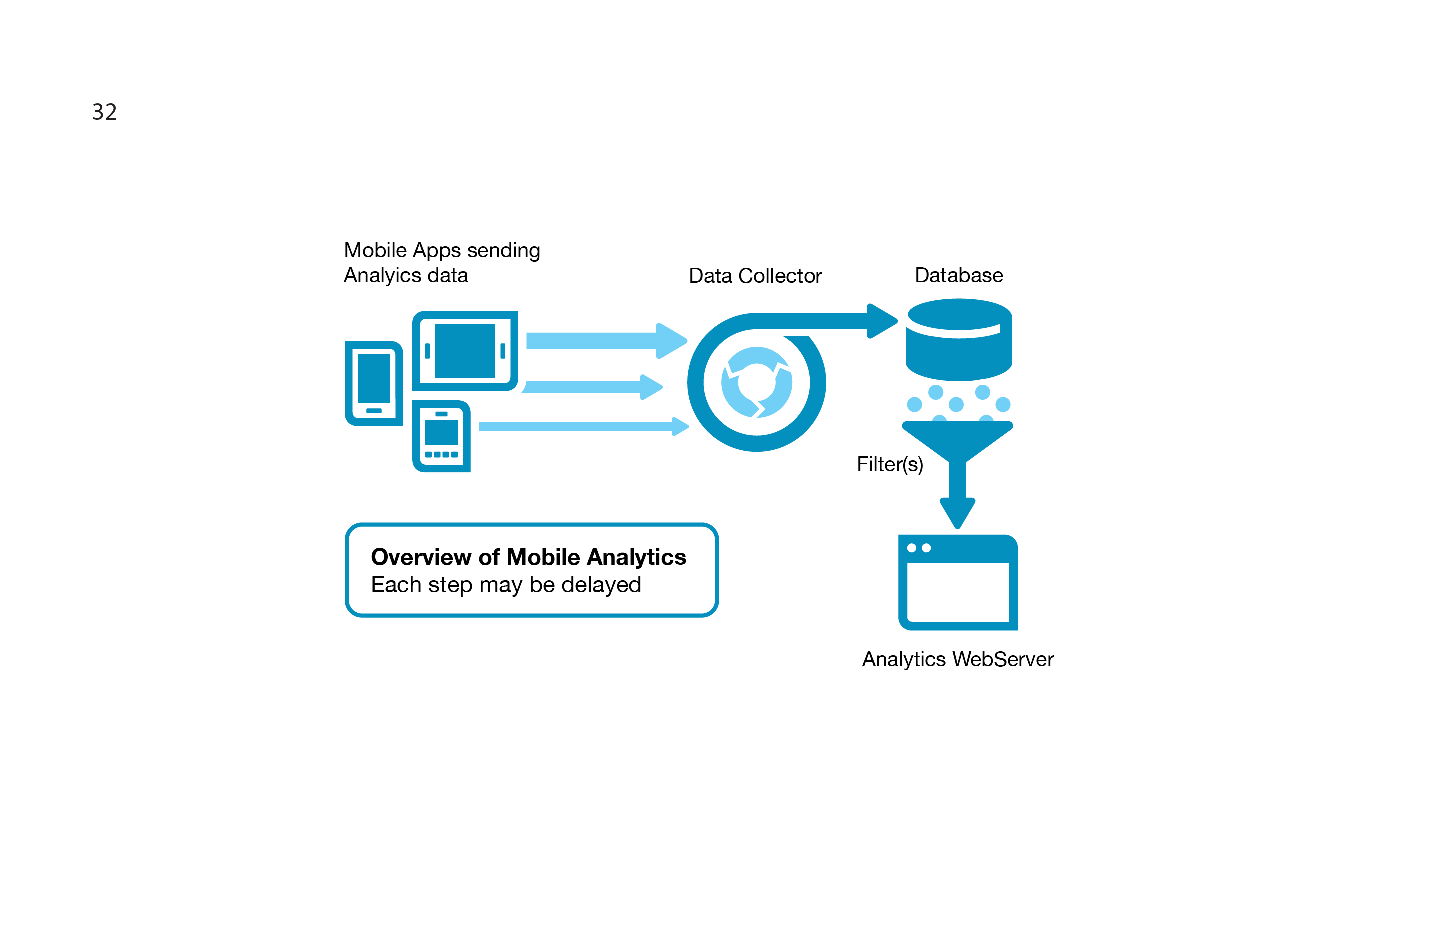
\includegraphics[width=\linewidth]{images/mobile-analytics-playbook/Chart-08-Overview-of-MobileAnalytics.pdf}
    \caption{Overview of Mobile Analytics~\cite{harty_aymer_playbook_2016}}
    \label{fig:map2016-overview-of-mobile-analytics}
\end{figure*}

An overview of Mobile Analytics was published in The Mobile Analytics Playbook,~\sidecite{harty_aymer_playbook_2016}, and the figure is reproduced here with permission in Figure~\ref{fig:map2016-overview-of-mobile-analytics}. The overall approach also applies conceptually in terms of how either apps (often delegated to the analytics library implementation) or the device sends the data. As an observation, the approach would also work if the data is transferred using other conduits, such as copying the data using a memory card, however these details are unlikely to apply to the vast majority apps and even for those developers the conceptual model is unlikely to change materially.

Transmission of the contents of the logs and/or mobile analytics data is asynchronous and may occur almost immediately, or in some rare cases months later. In a discussion on the Android implementation of the popular segment.io library, a non-profit reading app needs to store up to six months of reading analytics on the device using this library. The authors discussed practical ways to store the analytics events without loss and then to be able to upload them correctly even where network connectivity is unreliable~\sidecite{segmentio_supporting_6_months_offline}. Several analytics providers have documented their transmission mechanisms. \emph{``Crashlytics limits logs to 64kB and deletes older log entries when a session's logs go over that limit."} and it~\emph{``...only stores the most recent eight recorded exceptions. If your app throws more than eight exceptions, older exceptions are lost."}.  The non-fatal exceptions are sent the next time the app launches~\sidecite{firebasecrashlytics2020_customize_crash_reports}. In contrast the Segment implementation for Android stores up to 1000 events~\sidecite{segment_analytics_for_android_docs}.

One of the particular implementation details may be worth considering, which is the growth in intermediaries and their adoption by developers. Segment provides one such service, where they provide developers with a single per-client app API that then wraps hundreds of potential implementations and offers two \emph{``connection modes"}, device and cloud~\sidecite{segment_analytics_for_android_docs}. When using their cloud-mode~\emph{``Segment sends messages to the Segment servers, and then translates and forwards that data on to the downstream tools."} Their service becomes a vital additional component in the process and may affect many aspects of the data including privacy, who can analyse it, and latency implications.   

\subsection{Data funnels from users to devs}
The following list itemises a set of possible stages in a data funnel for data that originates from a user's device until it is available for use by the development team. real-world funnels are likely to include a subset of these, in a particular order in terms of the data flow.

\begin{itemize}
    \item Per-app implementation and options
    \item Per-analytics/logging library implementation and options
    \item Farming the log (and/or potentially other usage data) data on device
    \item Device model and operating system combination
    \item Per device implementation and options
    \item Data daemons that control/negotiate what data is and is not available/provided
    \item Data privacy screening (can occur at various points in the funnel)
    \item Batching, queuing, limits, latencies, transmission triggers, ...
    \item Connectivity quality and reliability
    \item Network behaviours e.g. where traffic may be blocked in some geographies, by some network providers, etc.
    \item Data Collector inbound processing (filtering, buffering, validity checks, non-repudiation, dealing with spoofing, fakes, etc.)
    \item Analytics tool filtering and reporting. This may include muting of some aspects of the reporting e.g. for issues considered no longer actionable. 
    \item Content access, storage, combination with other sources, further reporting, etc.
\end{itemize}

Note: there may also be data injected into the funnel, for instance through \href{https://en.wikipedia.org/wiki/Synthetic_monitoring}{synthetic monitoring}, testing of the apps and/or the analytics clients and APIs, spoofing, denials of service, and so on. 

MUST-DO add figure, write up this section.




\section{Conceptual model of usage analytics}
Usage analytics pertains to recording and analysing the usage of software. Application usage analytics is mentioned in various sources, including patents filed by Google in the USA~\emph{e.g.} for methods and systems to collect and provide application usage analytics to developers~\sidecite{googlepatent_hyman2016_collecting_application_usage_analytics}. 

Conceptually there appear to be four broad levels of usage analytics, these are illustrated in Figure \ref{fig:four-layers-of-analytics-for-mobile-apps} and described next. These four levels can be approximately mapped~\sidenote{The approximation is because software is not quite so cleanly cut into layers or levels. For instance app-level mobile analytics can be used to record many aspects of GUI activities, albeit unnaturally. Also, the operating system can observe aspects of the GUI, for instance by instrumenting the Accessibility APIs, a topic I touch on in one of the appendices.} to the three layers of an app:

%\akb{Are 'Visual' analytics tools automatically 'Mobile' tools as well? The \textit{heatmapping} example seems to be one that could fit into both layers}

Their use will be discussed in more detail in the chapter titled~\href{chapter-applying-analytics-to-development-practices}{\emph{\nameref{chapter-applying-analytics-to-development-practices}}}. %MUST-DO decide whether layer and level are synonymous, and if not whether to use one term or the other. Anyway I'm aware I may be conflating both terms here and want to improve the precision of whichever term(s) I use. 

\begin{figure*}
    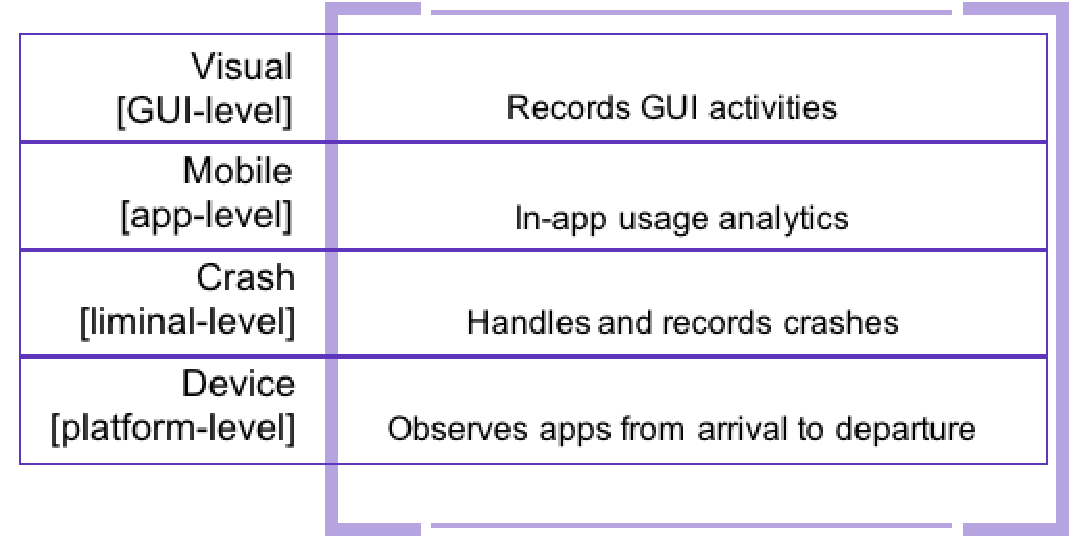
\includegraphics[width=\linewidth]{images/4-layers-of-analytics.pdf}
    \caption{Four Layers of Analytics for Mobile Apps}
    \label{fig:four-layers-of-analytics-for-mobile-apps}
\end{figure*}

\begin{itemize}
    \item \textbf{Visual (GUI-level)} operates at the GUI level, or layer, of the app. It records aspects of the GUI activities such as touches, gestures, interactions with the screen, and data entry. Often it includes recording what is on the screen too. A common type of Visual analytics is \emph{heatmapping} software. Note: visual analytics may be \emph{implemented} in the app, conceptually they observe the GUI as if from above the UI.
    \item \textbf{Mobile (app-level)} is incorporated as part of the app and records aspects of what the app is doing, in effect aspects of the usage of the app. Mobile Analytics is prevalent in Android apps and already used for various business purposes.
    \item \textbf{Crash (liminal-level)} is where specialised reporting can intercept crashes. Through the interception they can change the behaviour of the app, for instance to provide a better user-experience, log, and report the crash to the developers. \emph{Fatal crashes} are ones where the application quits. These can also be observed by the operating system; for mobile apps the operating system is an intrinsic part of the platform.
    \item \textbf{Device (platform-level)} Platform-level analytics can record apps from when they are installed until they are removed. This recording can include details such as when apps are in-use, crashes, freezes, and so on. Both of the dominant platforms (iOS and Google Android) allow users to decide whether their devices will share this data.
\end{itemize}

% https://new-wine.org/resources/blog/living-liminality-lessons-trust-gratitude-prayer-compassion-global-church-dd508239ff5

This research includes case studies and developer reports of examples of analytic tools that cover three of these four layers of analytics. The remaining layer, visual analytics, is described briefly with a few examples, visual analytics is seldom used in production mobile apps and therefore it was excluded these from the core research. They may be an interesting topic for future research particularly given some of the potential benefits of visual analytics. % COULD_DO add notes on privacy issues and other complicating factors in this sort of research. 


\section{Conceptual model for DevOps}
DevOps recognises the benefits of connecting development and operations of software. a Yin Yang symbol recognises there's some negative in the positive and vice-versa. Conceptually, teams can choose to invest in operations while they're developing to improve the operational aspects of their software, for instance by designing in good operability. Similarly when the software is in use by observing the software's behaviours operations can improve the development. Examples include: considering the how improvements could be developed or the software development lifecycle process improved based on how the software is being used.

\begin{figure}
    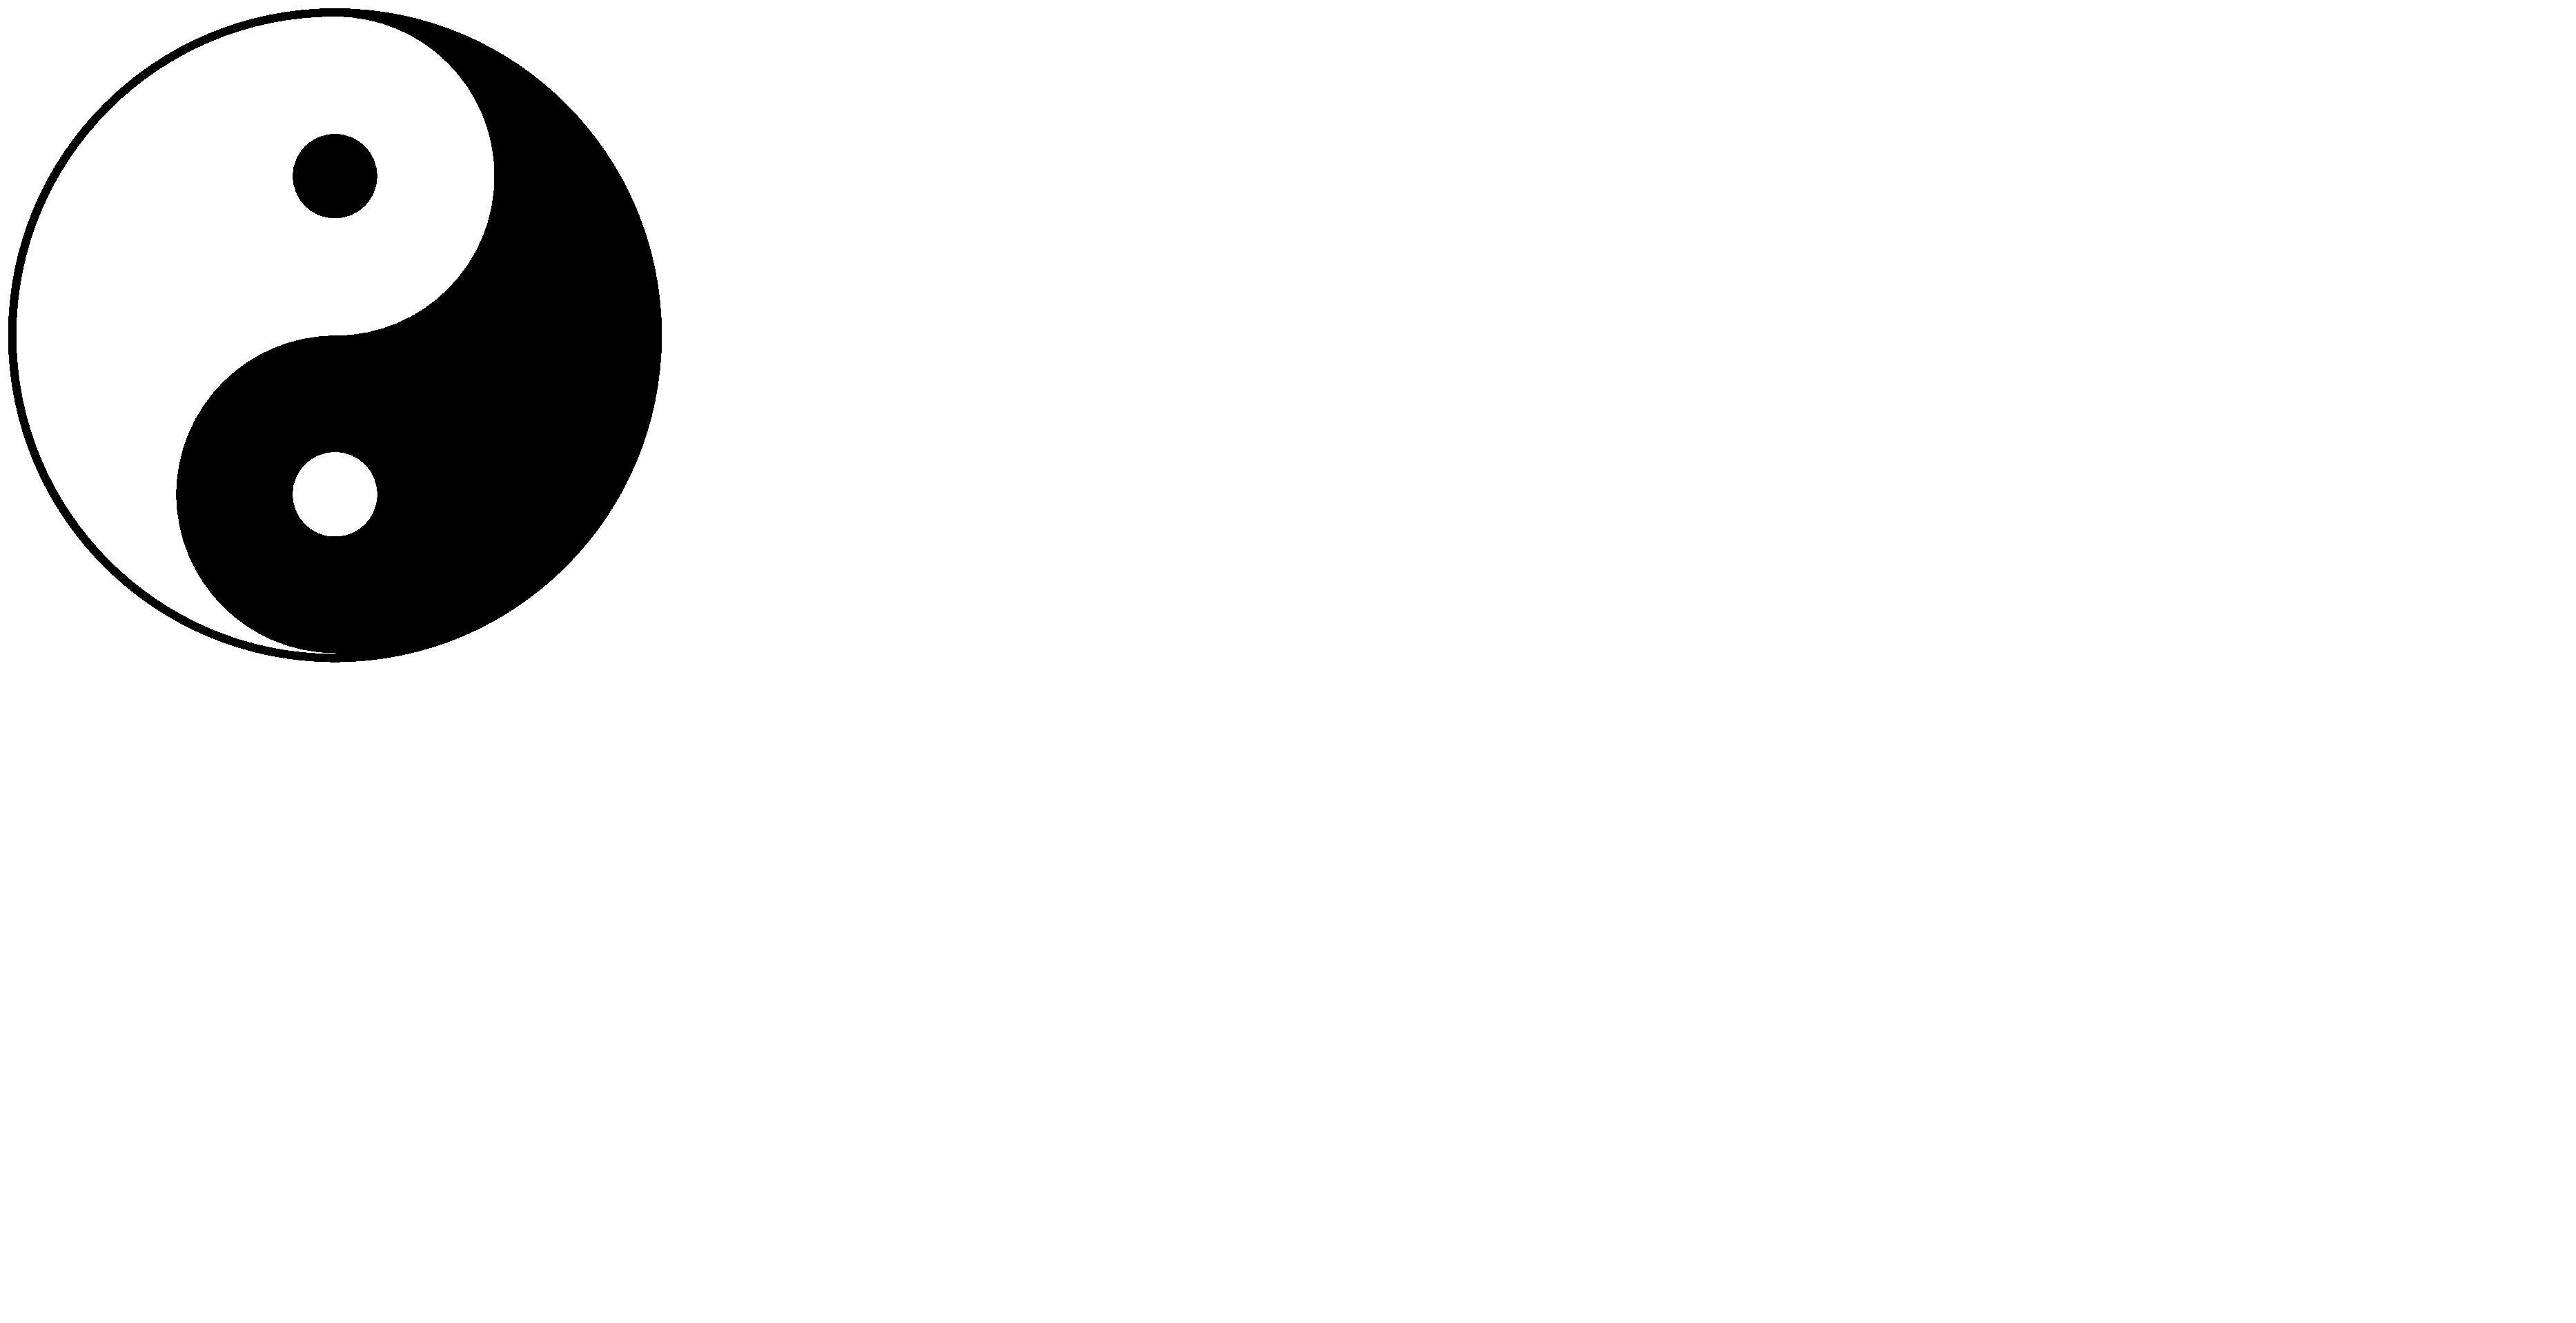
\includegraphics[width=0.5\linewidth]{images/wikipedia/Yin_yang.pdf}
    \caption{Yin Yang to represent DevOps}
    \label{fig:yinyang_for_devops}
\end{figure}



One of the popular concepts in DevOps is represented by an infinite loop in the shape of a horizontal figure of eight like diagram, illustrated in Figure~\ref{fig:atlassian-state-of-devops-report-2016-devopsloop}.~\sidenote{This example is from a blog post by Atlassian~\url{https://www.atlassian.com/blog/devops/2016-state-of-devops-report} announcing \emph{``The State of DevOps report"} 2016 edition.} There are many variations of this illustration available, perhaps unsurprisingly given the popularity of DevOps and those who write and publish on the topic who may want to give their own spin on the topic.

\begin{figure*}
    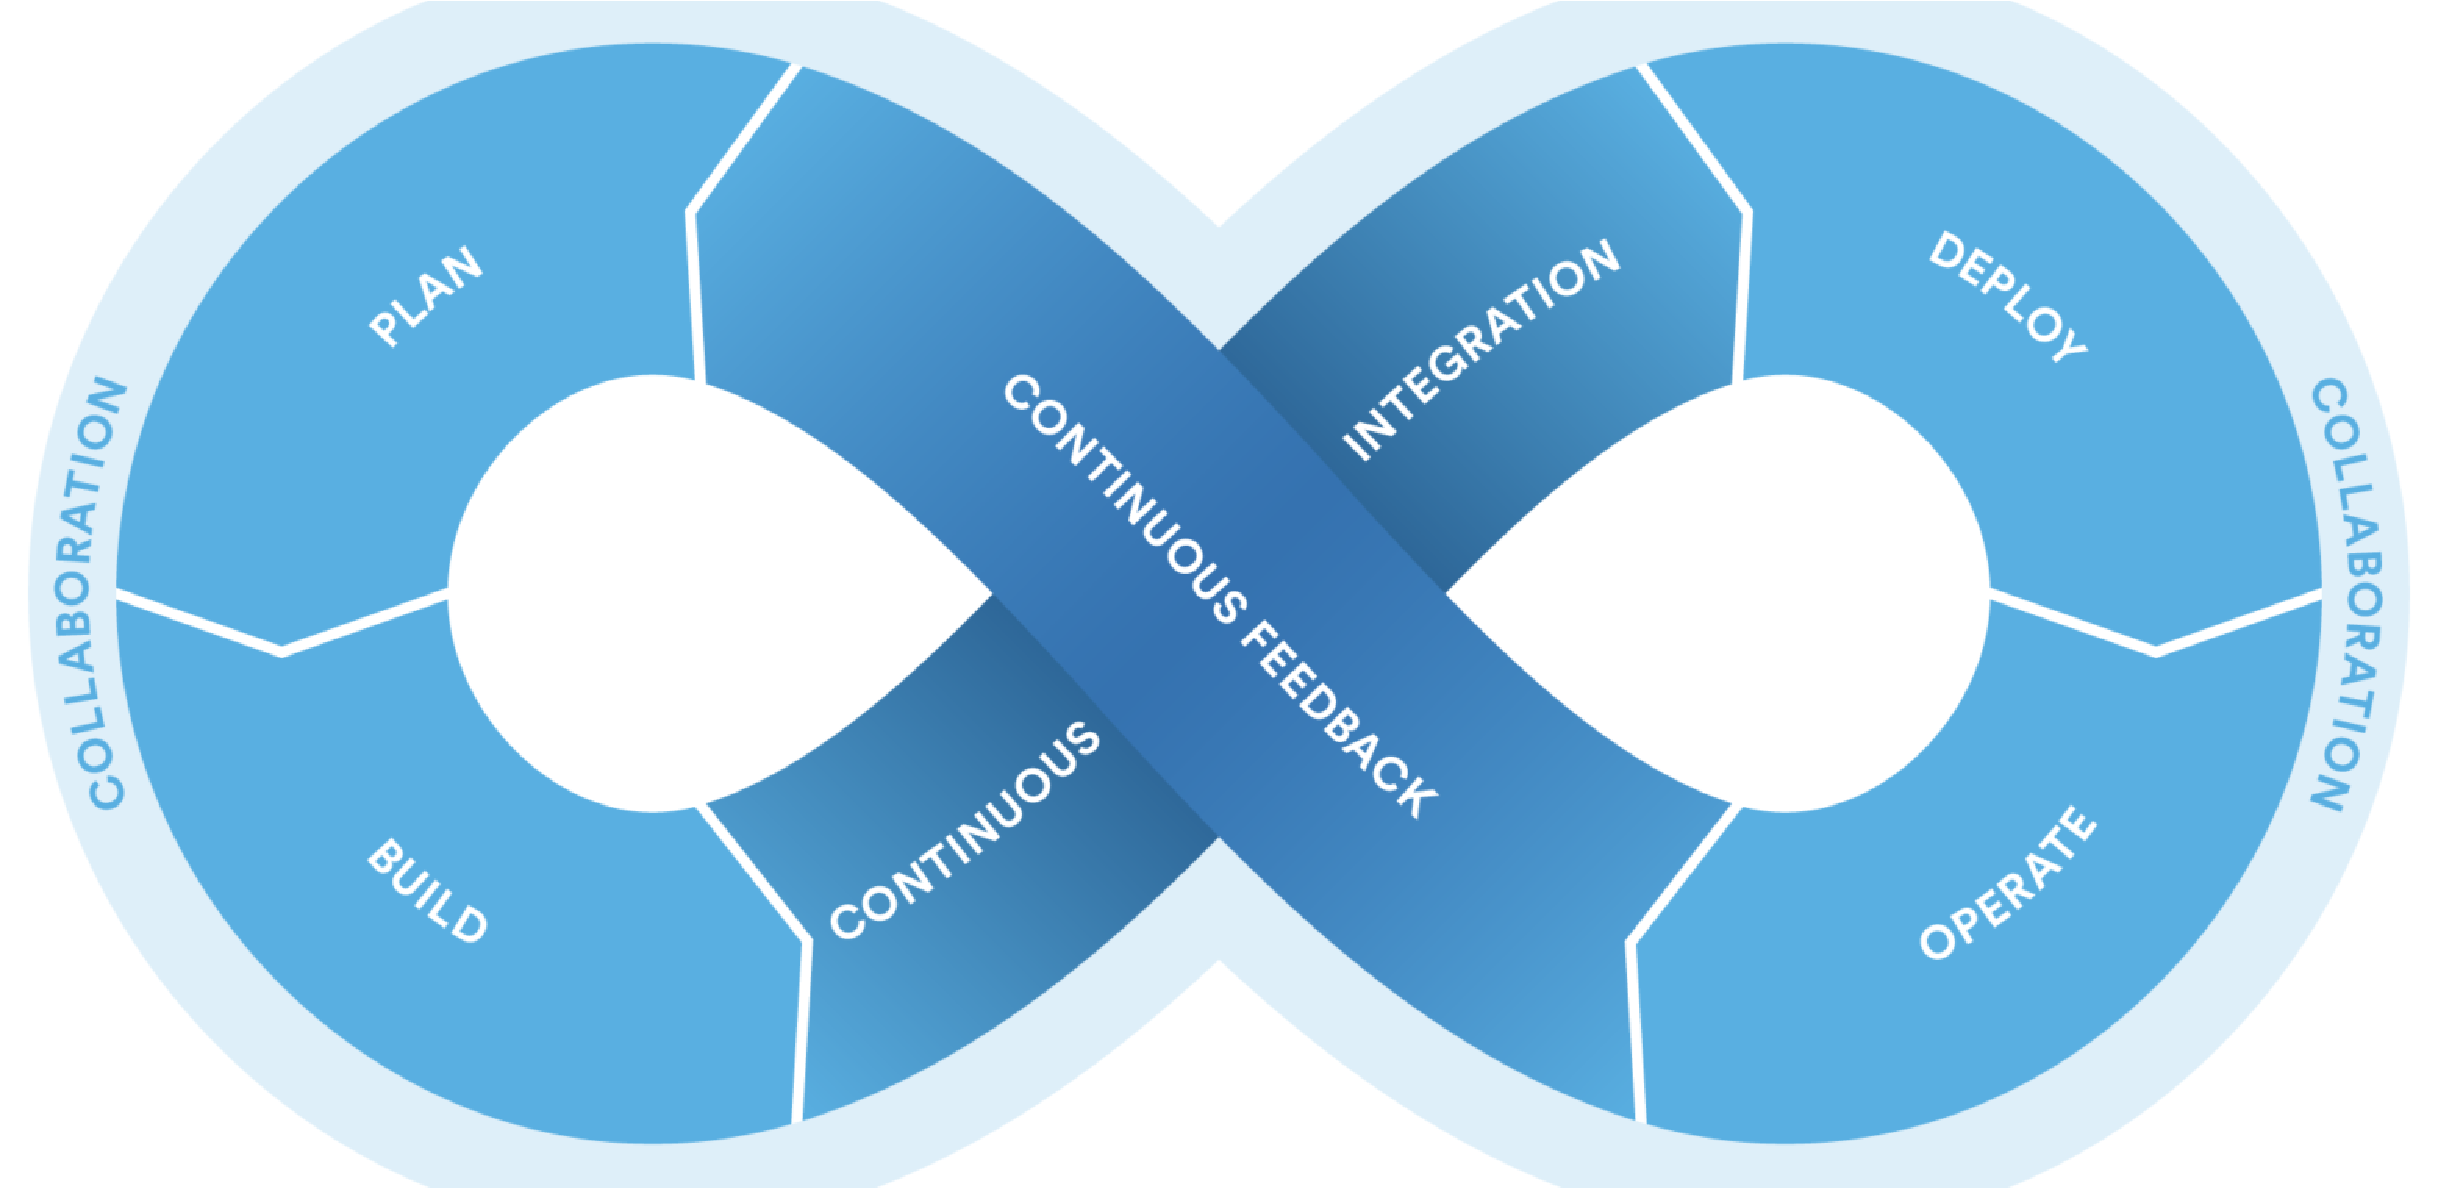
\includegraphics[width=\linewidth]{images/atlassian/atlassian-state-of-devops-report-2016-devopsloop.pdf}
    \caption{Atlassian DevOps loop}
    \label{fig:atlassian-state-of-devops-report-2016-devopsloop}
\end{figure*}
% https://3kllhk1ibq34qk6sp3bhtox1-wpengine.netdna-ssl.com/wp-content/uploads/devopsloop-1560x760.png



\section{From conceptual models to practicalities}
The previous sections introduced five conceptual models that help to establish the context for the ecosystem, structural aspects of mobile apps and perspectives where mobile apps can be observed, analogue and digital feedback, usage analytics and DevOps considerations. The next five sections cover various practical aspects of mobile apps including development and usage lifecycles, information sources and finally choices for engaging with analytics.


\section{Mobile apps and development team's mobile devices}
A mobile app is more than compiled source code, it includes various resources such as text, images, audio, screen layouts, and sometimes other contents. Many include software libraries from one or more sources. Mobile apps are also digitally signed. Data and information can be obtained for these various constituent parts, for instance some failures may occur within a library at run-time and be reported in logs and via mobile analytics.

Development team's mobile devices, with occasional exceptions are often the same device models that end users have and use; and furthermore they have similar end-user accounts and the majority of their apps are installed in similar ways to those installed on end-user devices. These similarities have some important implications - data on the usage of these devices by the development team may also be collected and considered as being part of the end-user population, and any in-app analytics in the various installed apps may provide their data to the respective mobile analytics systems,~\emph{etc.}

These devices may be configured differently and they may also run local builds and internal releases of apps. The apps may be configured to provide different amounts of information in local logs and/or using mobile analytics libraries for instance to either distinguish the usage or to suppress data from being shared. Knowing and understanding these nuances can help interpret some of the sources of data and information pertaining to these devices and apps.


\section{Mobile app development lifecycle}
To provide some context for this section, Figure \ref{fig:ci-cd-development-and-feedback}~\sidenote{Reproduced from \emph{``An empirical study of architecting for continuous delivery and deployment"}~\cite{shahin2019empirical_study_architecting_cd}}
illustrates a modern continuous software lifecycle including feedback. We can observe several distinct stages in the development and deployment of software and the feedback each stage can provide. %MUST-DO check the guidelines for reproducing and citing a figure as-is.
%
In contrast, Figure \ref{fig:google-play-app-development-and-feedback} illustrates a similar software lifecycle for Android apps released through Google Play together with the various forms of feedback~\sidenote{Here we have excluded feedback from the app store, nonetheless it exists for many app stores.} 

Key differences between typical CI/CD lifecycles and the one for Google Play is the pre-launch testing and the app store providing both user feedback and a service called Android Vitals. The pre-launch reports are generated automatically by Google where the app store runs automated monkey testing on a farm of Android devices and various static analysis checks of releases deployed to any of the test channels. They are described in~\href{subsection-test-channels}{Test Channels}. %MUST-DO actually add information on the test channels and how releases can be promoted to production releases in Google Play.


\begin{figure*}
    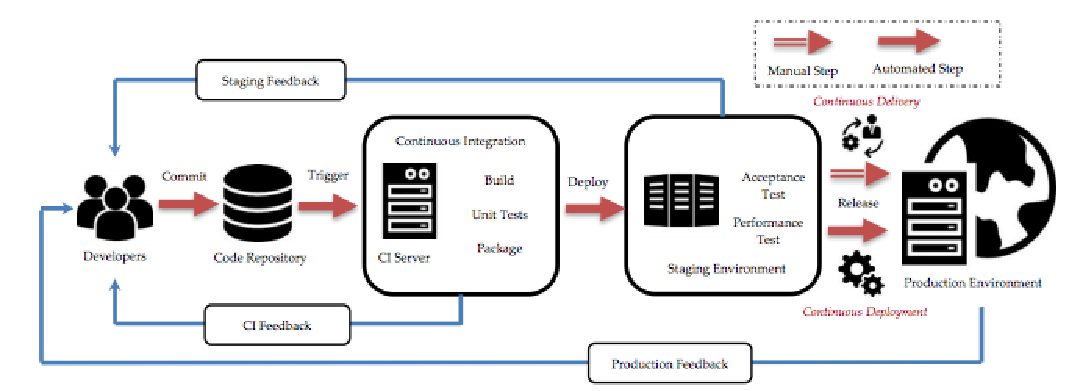
\includegraphics[width=\linewidth]{images/ci-cd-development-and-feedback.pdf}
    \caption{CI/CD development and feedback, reproduced from~\cite{shahin2019empirical_study_architecting_cd}}
    \label{fig:ci-cd-development-and-feedback}
\end{figure*}

There are additional sources of \emph{analogue feedback} from people, including from alpha and beta testers and end users; and \emph{digital feedback} from Google tools and from usage data collected from the field. These terms are expanded in the section~\href{analogue-and-digital-feedback}{\emph{\nameref{analogue-and-digital-feedback}}}.

% Vel This figure doesn't appear in the generated PDF file. I don't think I've used minipages (at least not earlier in this chapter) David Carlisle proposes https://tex.stackexchange.com/a/85153/88466 to help find the missing float, however I still don't understand the cause of the missing float.
\begin{figure*}
    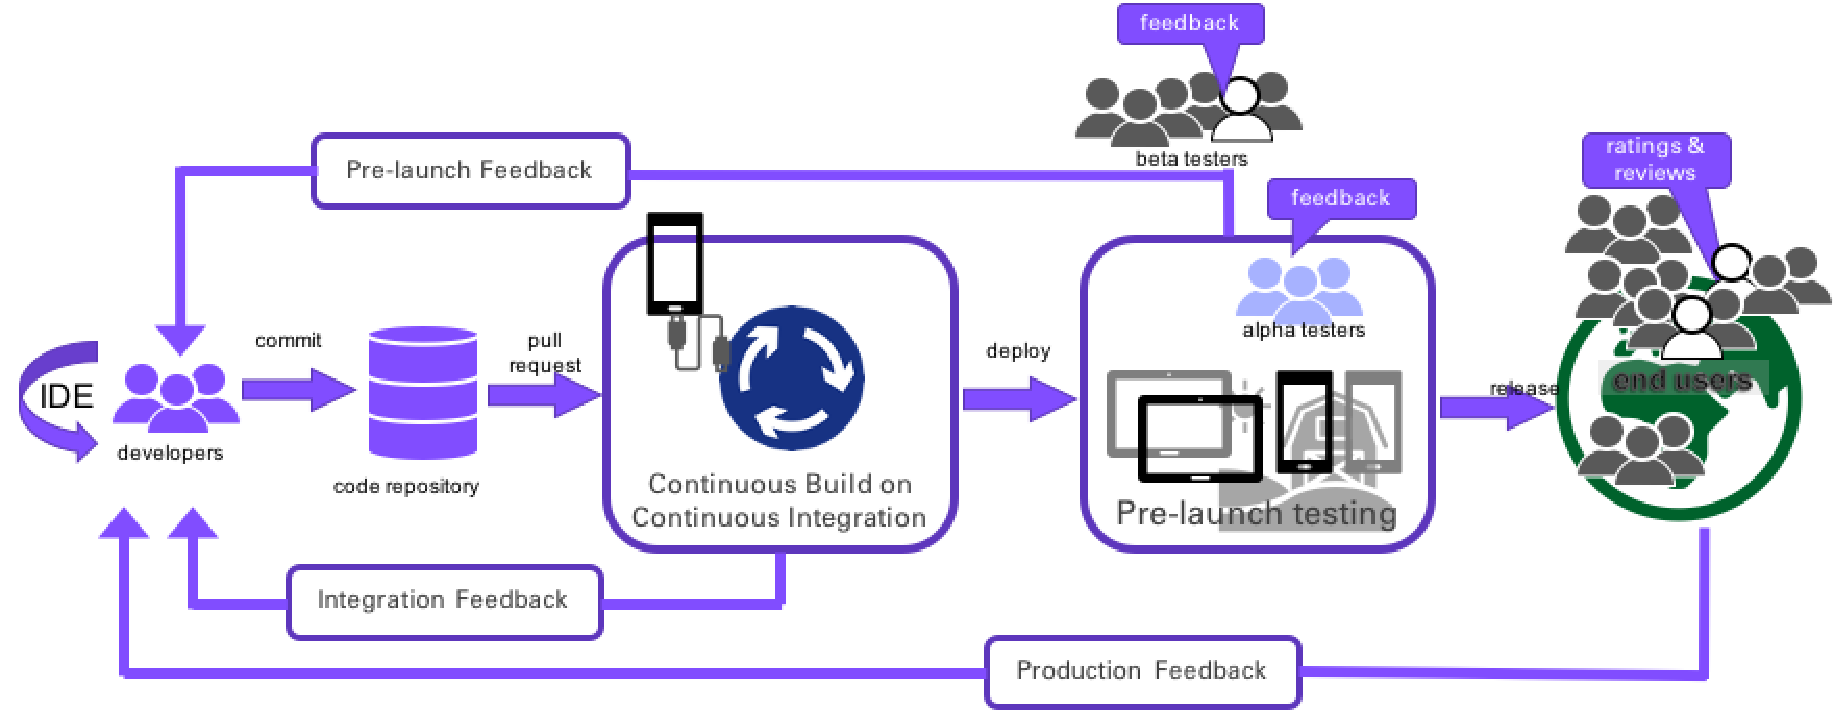
\includegraphics[width=\linewidth]{images/google-play-app-development.pdf}
    \caption{Google Play App Development and Feedback}
    \label{fig:google-play-app-development-and-feedback}
\end{figure*}


\section{Mobile app usage lifecycle}
Mobile apps have a usage lifecycle, which starts when an app is chosen to be installed and ends with either abandonment or active removal of the app from a device. Figure~\ref{fig:mobile_app_usage_lifecycle}~\sidenote{Based on a figure in~\cite{bohmer2011falling_asleep_with_angry_birds}} illustrates the possible stages of a mobile app's life on a user's device. Google Play Console collects data consistent with this lifecycle, analyses it and provides aggregate reports based on their analysis. 

For clarity and completeness there is another lifecycle when the app is running, described in the Android documentation as the \emph{``Processes and Application Lifecycle"}~\sidecite{android_processes_and_application_lifecycle} These are more detailed and are not included in the reports Google provides developers. %(I doubt their details would be recorded either). 
Note: the processes and application lifecycle may affect how in-app analytics libraries behave, including when they transmit their data to their respective central servers.

% More info and code samples: https://www.vogella.com/tutorials/AndroidLifeCycle/article.html

\begin{figure*}
    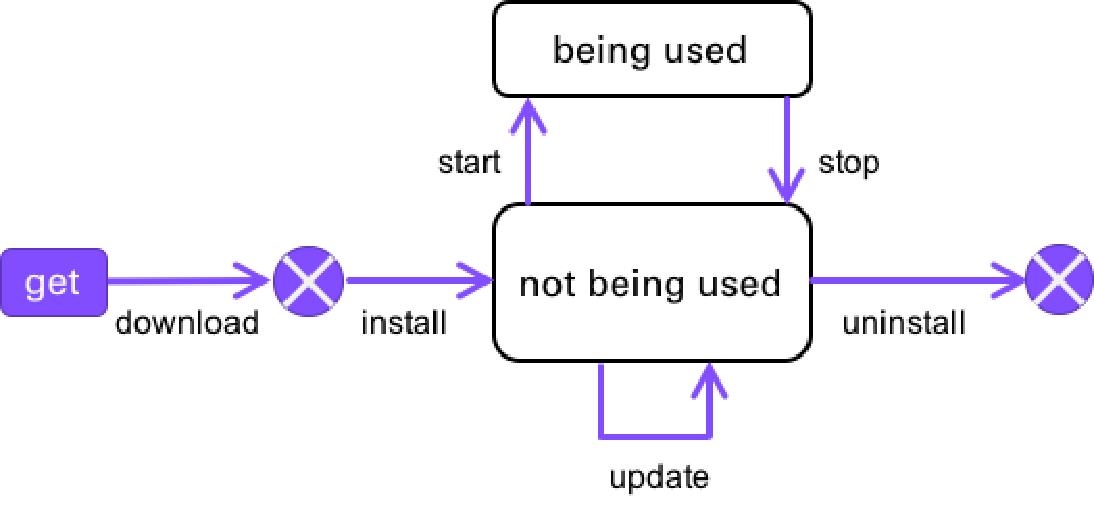
\includegraphics[width=\linewidth]{images/mobile_app_usage_lifecycle.pdf}
    \caption{Mobile App Usage Lifecycle}
    \label{fig:mobile_app_usage_lifecycle}
\end{figure*}

A later section~\href{sec:platform-level-analytics}{\emph{\nameref{sec:platform-level-analytics}}} provides a proposal of how Google collects the underlying data (they do not document, explain or encourage research in how their system works, We return to their (Google's) reported behaviour and the effects later in this thesis). % MUST-DO add link to: Developers banned from app store ecosystem and their apps removed.
And the chapter \href{app:software-contributions}{\emph{\nameref{app:software-contributions}}} describes software we developed to help collect data from Google Play Console in order to facilitate both research and to enable developers to collect and use data...

Crashes are often considered a concrete measure of poor performance of software and there has been extensive research in crashes for Android applications, in particular. I suspect there are various reasons for the focus on crashes as an oracle for testing software, crashes are unambiguous (even if the causes are not) and they are also binary so easy to determine whether software has, or has not, crashed. 

In 2017, Google launched a service called Android Vitals as a new, intrinsic part of Google Play Console,~\sidecite{googblogs_I_O_2017_everything_new_in_the_google_play_console}, where they popularised a measure called \emph{Stability} to assess the quality of Android apps. Their measure includes both crashes and when an application freezes or is unresponsive for at least 5 seconds from a user's perspective, a term Google call Application Not Responding (ANR).


\subsection{DevOps for mobile apps}
This section starts with an overview of DevOps concept of an infinite loop for software generally before becoming more specialised on DevOps for mobile apps. %SHOULD-DO consider expanding this section. TBD how much I should write about the concepts and terms. 
The focus here is on data from various stages of a conceptual infinite combined development and operations process to indicate where mobile analytics applies in terms of providing data to the development team. This data includes: log data, static analysis results, test results, release and usage data, and mobile analytics data and reports.

In October 2020, one of the students taking part in the PhD symposium at the ICST2020 conference presented a variation of the DevOps loop (as illustrated earlier in this chapter in Figure~\ref{fig:atlassian-state-of-devops-report-2016-devopsloop}) that is relevant to this research. In the student's figure their focus was on crash reproduction and this illustration is temporarily illustrated in Figure~\ref{fig:crash-reproduction-icst2020}(~\emph{pending an update from the presenter of that topic}).

\begin{figure*}
    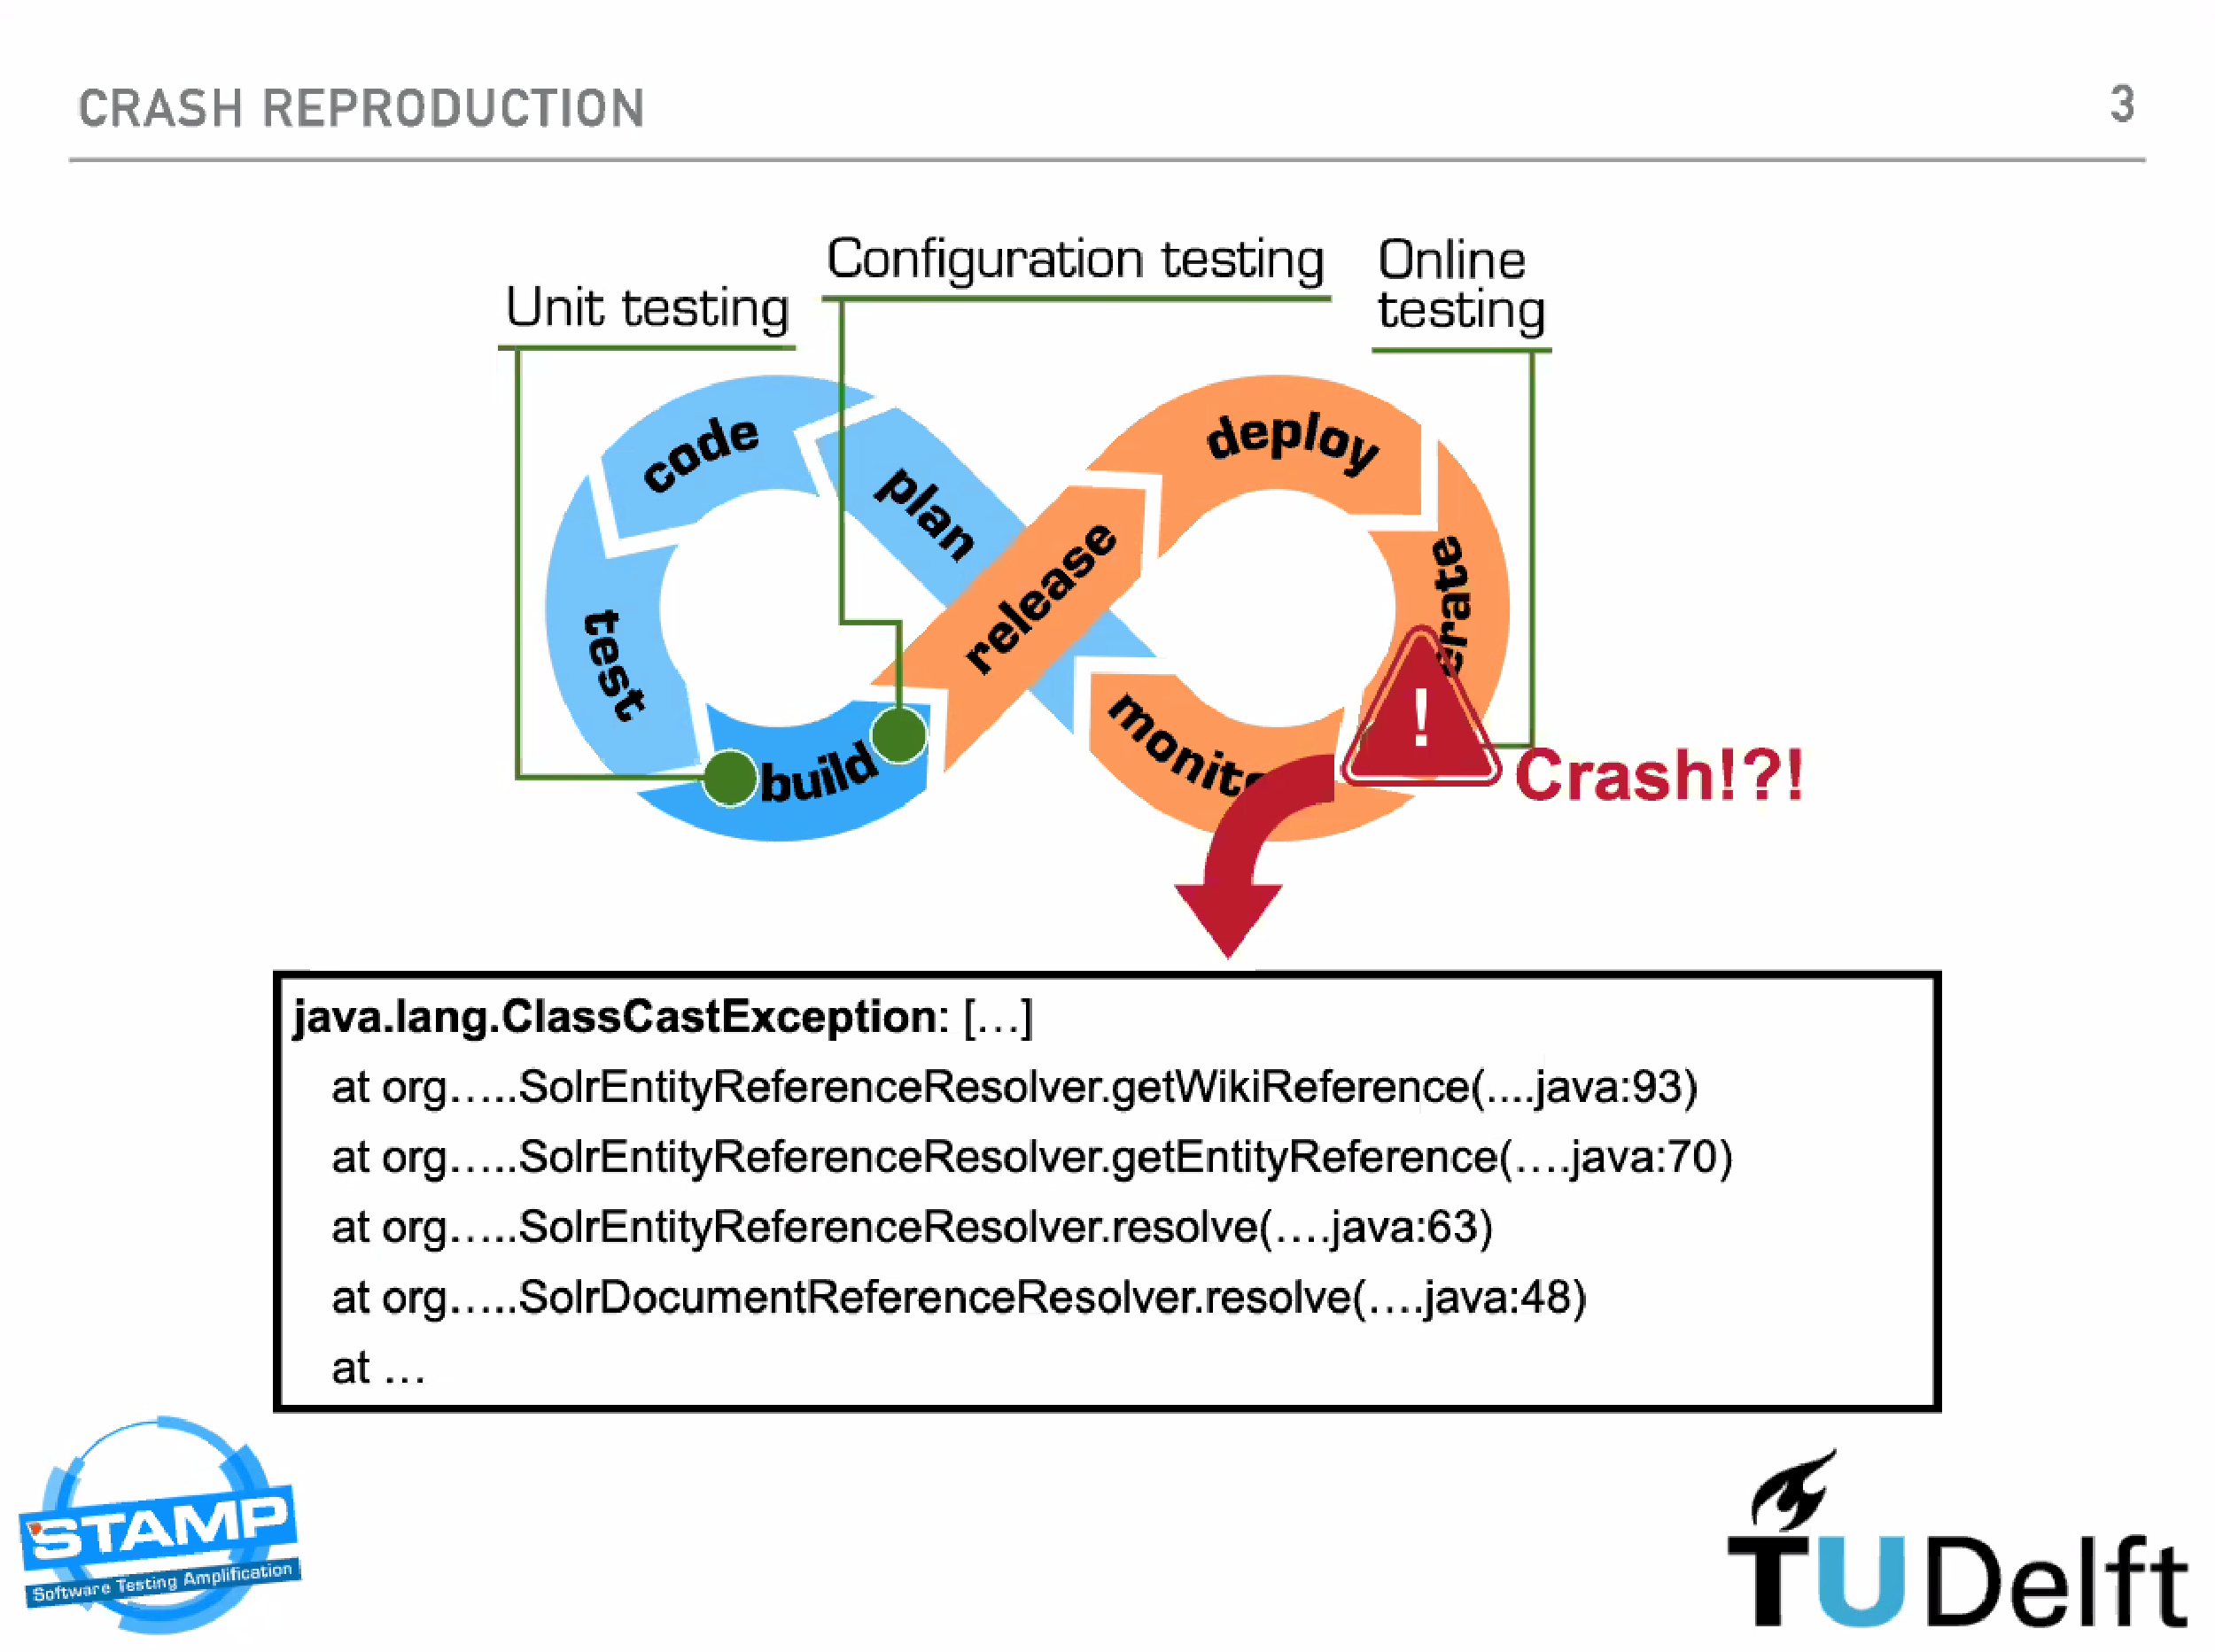
\includegraphics[width=\linewidth]{images/icst-2020/crash-reproduction-icst2020.pdf}
    \caption{Temporary image: Crash Reproduction}
    \label{fig:crash-reproduction-icst2020}
\end{figure*}

Figure~\ref{fig:oberve-and-apply-devops-loop} is revised illustration that shows, in red, the extent software can be observed, and in green of when the results of those observations can be applied to the code. Note: the observations can be applied throughout every phase, for instance during deployment aberrant behaviour observed during the deployment may lead to the deployment being paused.

\begin{figure*}
    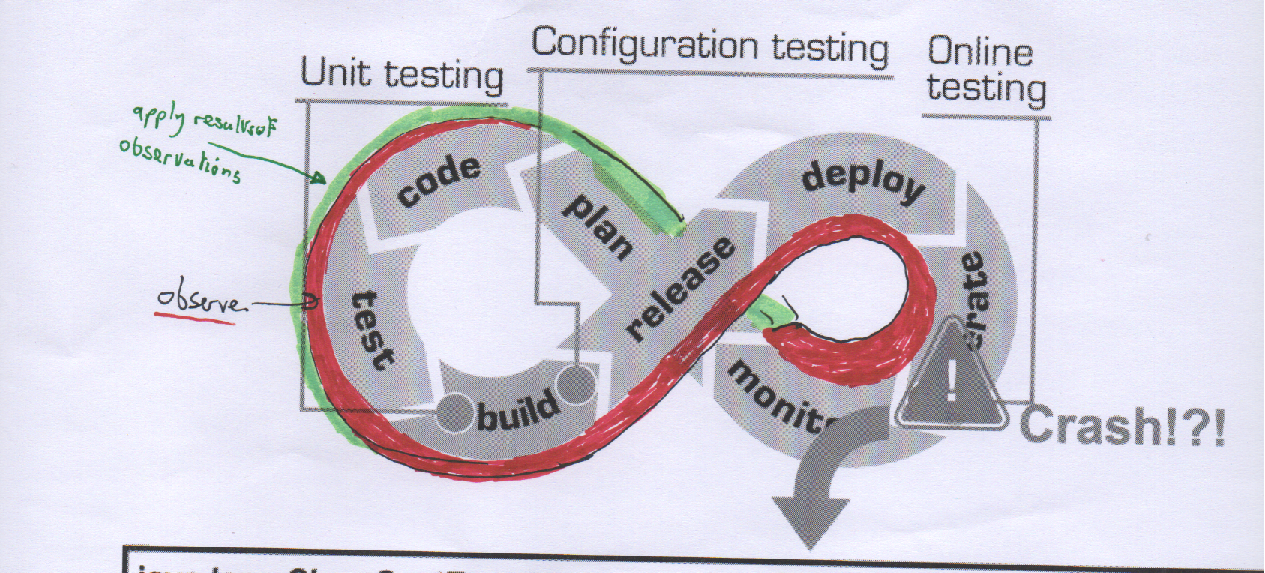
\includegraphics[width=\linewidth]{images/rough-sketches/hack-of-devops-crash-figure.pdf}
    \caption{Rough Sketch: Concept of feedback on software and applying it}
    \label{fig:oberve-and-apply-devops-loop}
\end{figure*}

Data is available using various sources about software from the outset of coding until the software dies; however for the purposes of this thesis the focus is on when the software is actively used and maintained, as illustrated in the previous three figures:~\ref{fig:atlassian-state-of-devops-report-2016-devopsloop},~\ref{fig:crash-reproduction-icst2020},~\ref{fig:oberve-and-apply-devops-loop}. 

During coding code analysis tools such as static analysis identifies patterns of potential concern in the source code and similar artifacts such as GUI layouts, strings in resource files, and so so. Tests can also be created and performed from the outset of the coding to provide runtime feedback (~\emph{i.e.} data) about the software under test, and similarly developers can add logging statements and also use logging built into the operating system that both provide data that can be mined to learn about the software's behaviours.

The build process may include configuration details, for instance to create a range of custom applications, to include instrumentation, to compress and obfuscate the application binary, and to create debug and release editions of the software. Data about the build process and about what has been built may also be observed and analysed and the products tested and analysed; for example an application binary can be scanned for information leakage in an obfuscated build, and builds can be tested to provide more data about how the software performs.

The release and deployment phases will be covered in more detail in the next section; here the focus is on the data available as part of these phases. 

As software is released the software transitions from being within the view of the development team to being used by others where the development team no longer has direct access to the devices that have the app installed or being used. They are remote from the use of the app. This means that local access to devices (to see what's happening and to try things out) and to the device's logs are unlikely to be practical, other sources of information now need to take precedence.

The release of a mobile app using an app store is subject to the processes and controls applied by the provider of the app store. The app store may offer both free and paid-for optional services to the developer, for example Google provides optional, free pre-launch reports that contain the results of automated testing and static analysis of application binaries. The app store may provide reports to the development team particularly if they decide to delay or block a release or suspend an app from being downloaded by end-users.

Usage is the ultimate active phase for a mobile app installed on a user's device. Simplifying slightly, as some apps run automatically in the background, most apps are started and used by end-users. Aspects of the usage can be recorded by various software utilities, in particular by the platform which records when an app starts and when it terminates. The platform can also record when an app is installed, when it is updated, and when it is uninstalled. The app store may provide developers with reports and statistics on the app's install base and usage. The app store may also provide developers with information about the performance of the app including any failures of the app while it was running.

Crashes are logged locally by the platform, some platforms may also record other failures and performance related data as well as resource utilisation and various capacities such as battery level locally. The platform may have permission from end-users to forward a copy of the information logged locally on the device and to use it for various purposes.  

\subsection{Software releases for mobile apps}
For mobile apps, the release management may include deployment of the app to end-user's devices either as a fresh install for new users or as an update for existing users that app on a given device~\sidenote{Mobile apps for Apple and Google app stores are installed per device and licensed per user so users can freely choose how many devices to install an app on, and they may even have different releases of the same app on different devices.}.

Releases may be acute or chronic in nature. Acute releases are actioned immediately and deployed as soon as practical. Chronic releases may involve alpha (closed-group membership) and beta (open-group membership) testing followed by rollout in stages, for instance starting at 10\% of the user-base, then increasing to 25\%, and so on until the new release is available to 100\% of the user-base. Note: there is no guarantee that the new release will be deployed to the entire user-base, and in my experience some users will keep using much older releases for as long as several years after newer releases were made available to them. 

The actual deployment and market penetration of a new release depends on several factors which may be outside the developer's direct control. This particularly applies for mobile apps made available through an app store where the app store and end-users can block new releases being applied. In my experience across a range of Android apps, for a 100\% rollouts it takes about a week for the new release to be installed on 50\% of the user-base's devices, however the range varies from 3 days to several weeks to reach 50\%.  

\begin{figure*}
    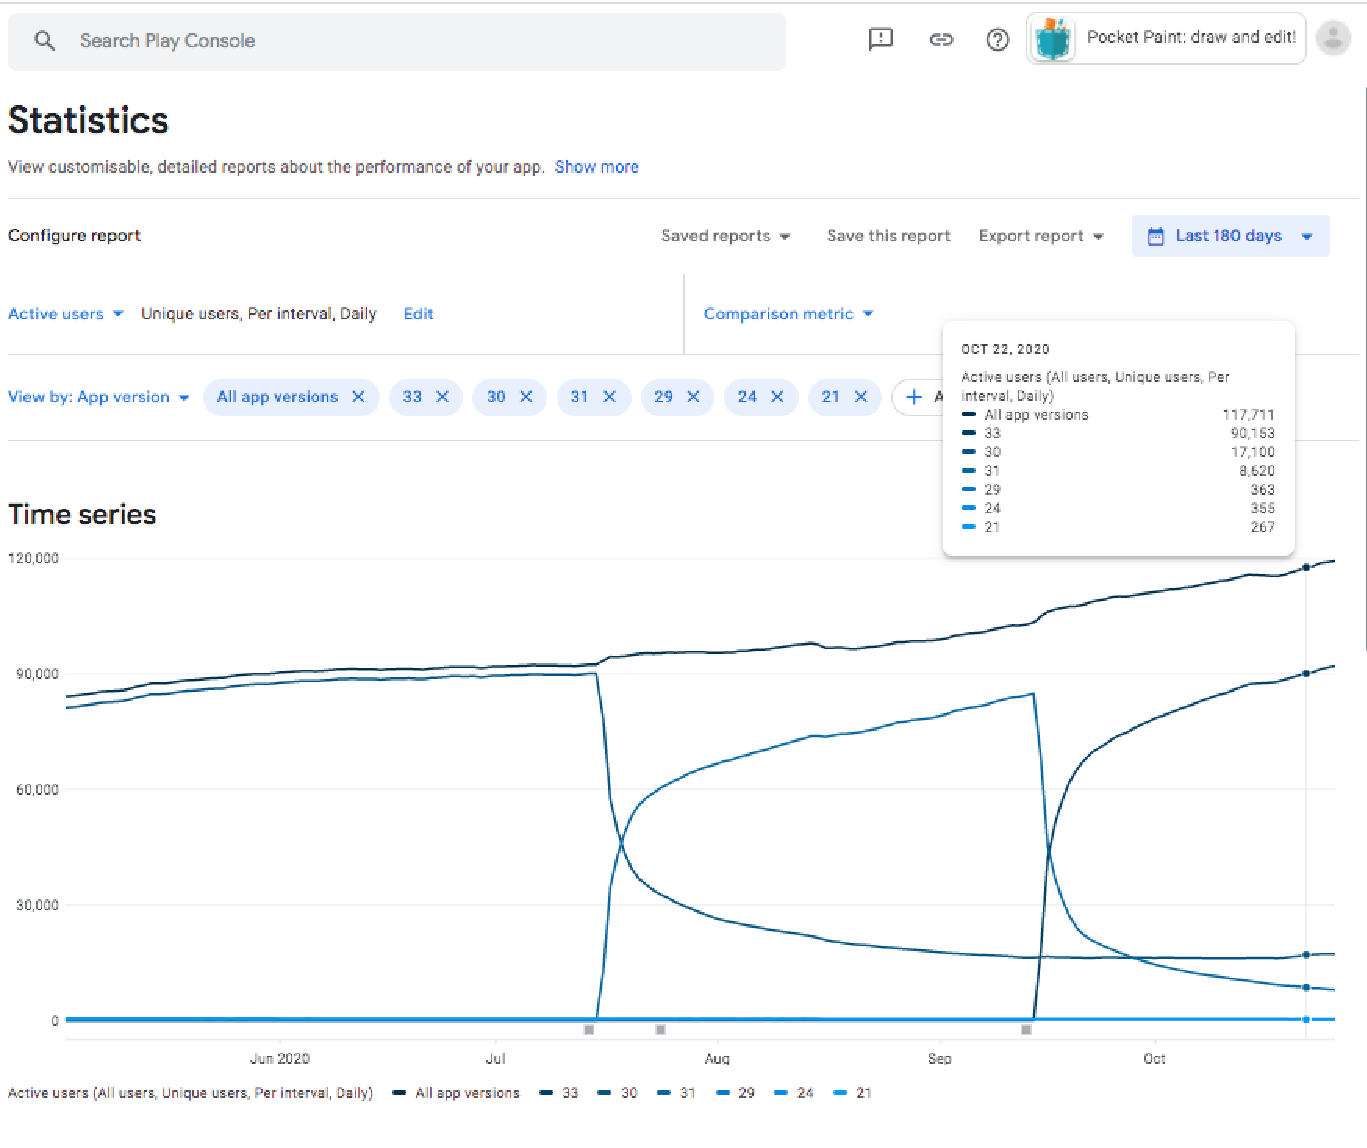
\includegraphics[width=\linewidth]{images/android-vitals-screenshots/catrobat/PocketPaint-ActiveUsers-180days-2020-10-29.pdf}
    \caption{PocketPaint Active Users 180 days by app version}
    \label{fig:pocketpaint-180d-active-users}
\end{figure*}

Figure~\ref{fig:pocketpaint-180d-active-users} illustrates a typical pattern of the majority of the userbase migrating from one app release to another and yet others remain with older releases during this period of 180 days (apologies for the small text in the image it was impractical to resize it adequately). Note: Google defines active users as:~\emph{``
The number of users who have your app installed on at least 1 device that has been turned on in the last 30 days"}~\sidenote{Text extracted from the online help for the `Active users' contextual help icon in Figure~\ref{fig:pocketpaint-180d-active-users}.} so it's not necessarily those who use the app in this period. The residues of users who remain on older releases of the app constrains the rate of change of the overall statistics as measured by Google Play Console and Android Vitals. This means that old buggy releases may continue to adversely affect the overall stability metrics for the app for long periods, even for months and years. Conversely, the project team may have addressed some of the causes of poor stability yet don't have a viable way of proposing users upgrade to the newer releases, and sometimes newer releases may have undesirable features or characteristics from an end user's perspective.

\begin{figure*}
    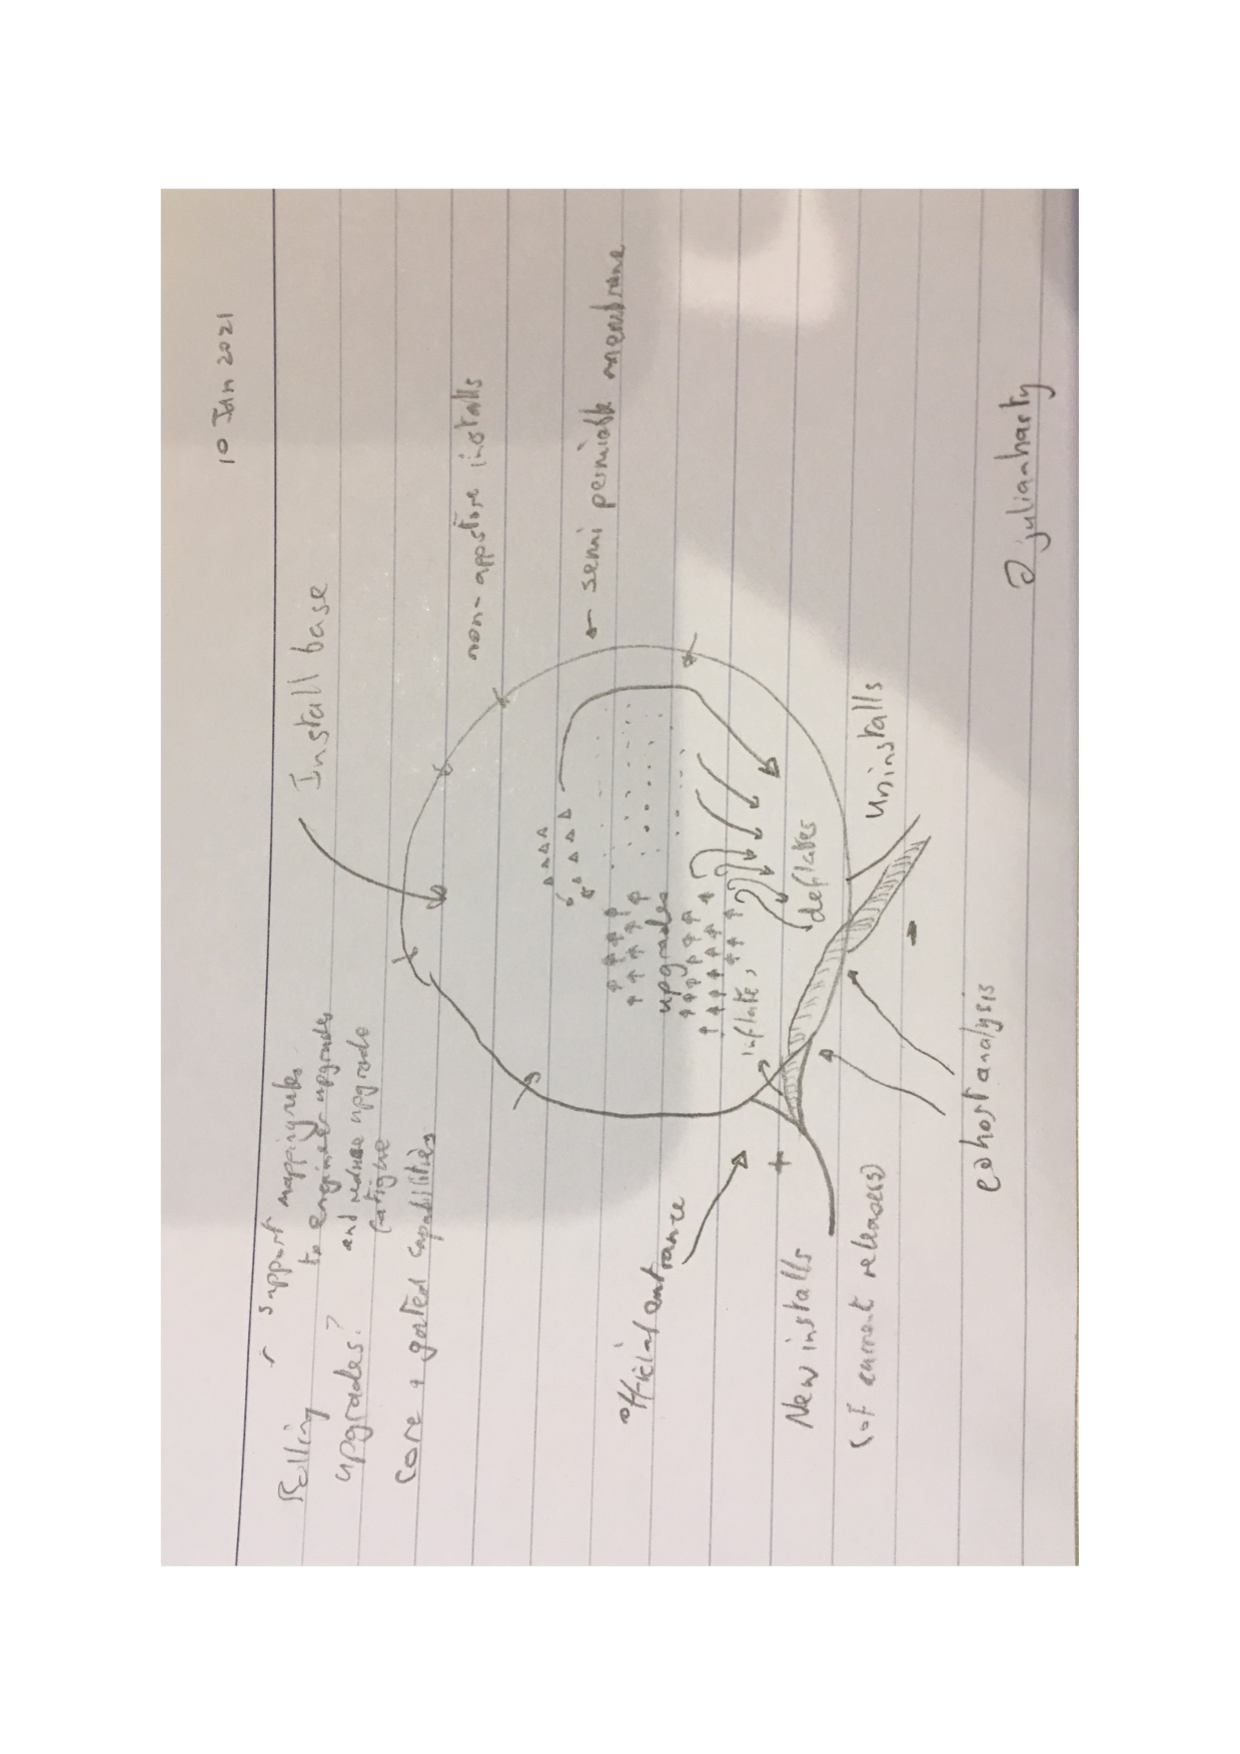
\includegraphics[width=\linewidth]{images/rough-sketches/app-install-base.pdf}
    \caption{App install base}
    \label{fig:app-install-base-rough}
\end{figure*}

\textbf{Installation base}: The rough sketch in Figure~\ref{fig:app-install-base-rough} illustrates static and dynamic aspects of the installation base for a mobile app. The approximate circle contains the installation base for an app. The size ebbs and flows based on new installs - which inflate the shape, and uninstalls - which deflate it~\sidenote{Note: apps may be downloaded independently of devices, for instance using a web browser~\cite{norwied2012_download_android_install_files}, and they may be installed independently of an app store. Both these traits may affect the accuracy of the installation counts.}. 

In current mainstream app stores users do not get a choice of which release of an app they will receive when they receive it, that choice is made by the app store using one or more releases provided by the developer. The app store may allow developers to choose various criteria for current releases, such as a percentage rollout, and then apply that on behalf of the developer. The boundary may be considered semi-permeable as some installations are not sourced from the app store. A key consideration is that upgrades apply to the install base so they occur within a population and do not change the number of installs. That said they may lead to decreases in the installation base for various reasons. Some users may uninstall an app prompted by learning of a new update of the app - for instance if it requires permissions the user considers intrusive or unsafe; others may uninstall the app after the update, for instance if they believe it is too buggy to merit using. Note: they are not able to revert to an earlier release within the current major app store's practices / constraints. 

To sum up so far, new installs receive the most current release gated by the rollout algorithms implemented by and in the app store. Upgrades also receive the most current release gated by the same rollout algorithms.

\textbf{Cohorts}: represent a group of users who share something in common and measures at intervals through time. Examples include new users who install the app on a particular day or in a particular week. They are used in analysis, for instance to measure what proportion of new users still have the app installed a week later. Cohorts can also be used to group users with a distinct release of an app, and so on. Useful introductions to cohort analysis using Google Analytics are available online~\sidecite{codehouse2020_cohort_analysis, googleanalytics2021_the_cohort_analysis_report}, and cohorts are used in various analytics tools including Google Analytics and Firebase Analytics. 

% https://www.codehousegroup.com/insight-and-inspiration/digital-strategy/cohort-analysis-and-how-to-use-it-in-google-analytics
% CHEST journal: Cohort Studies https://doi.org/10.1016/j.chest.2020.03.014

One reason why users uninstall an app is because of poor quality behaviours by the app. In a survey by Dimensional Research, 3011 participants completed an electronic survey to identify key factors that led to end user satisfaction with mobile apps. The research also `... sought to determine what users did when they were unsatisfied with a mobile app.' (page 5). 
53\% of respondents have uninstalled or removed mobile apps that regularly crashed, stopped responding or had errors and 37\% stopped using the app (page 16)~\sidecite{dimensionalresearch2015_mobile_app_use_and_abandonment}~\sidenote{The report is free of charge upon request: \url{https://techbeacon.com/resources/survey-mobile-app-users-report-failing-meet-user-expectations}}.

To sum up again, the installation base relies on a combination of existing and new users. Updates can lead to some existing users uninstalling the app - a topic to consider when planning releases of the app. Cohorts can be used to measure the effects of new releases of an app and several analytics tools already use them for tracking the retention of new users. Poor quality of an app may lead to more uses abandoning and even uninstalling the app. As a hypothesis: if an update of an app improves the quality of an app for a user the user may be pleased with the update and continue using the app, conversely if an update does not improve the quality of the app for that user some users will merely stop using the app others will actively deinstall it. Releases can be a point of inflection in terms of the userbase.

\textbf{Forced updates?} Some developers, and some platforms, may incorporate mechanisms to encourage or even try to force users to update their apps. However, doing so may upset and alienate some users. One of the case studies,~\href{study-greentech-apps}{\emph{\nameref{study-greentech-apps}}}, has used these mechanisms and this topic will be expanded in that case study. In contrast, the Kiwix Android app has over 70 releases being reported as active in a 7 day period, some several years old. Figure~\ref{fig:kiwix-30d-active-users} shows the overall active user base and the top ten of the 70+ releases according to Google Play Console~\sidenote{Google Play Console limits the graph to ten items on the secondary category.}.

\begin{figure*}
    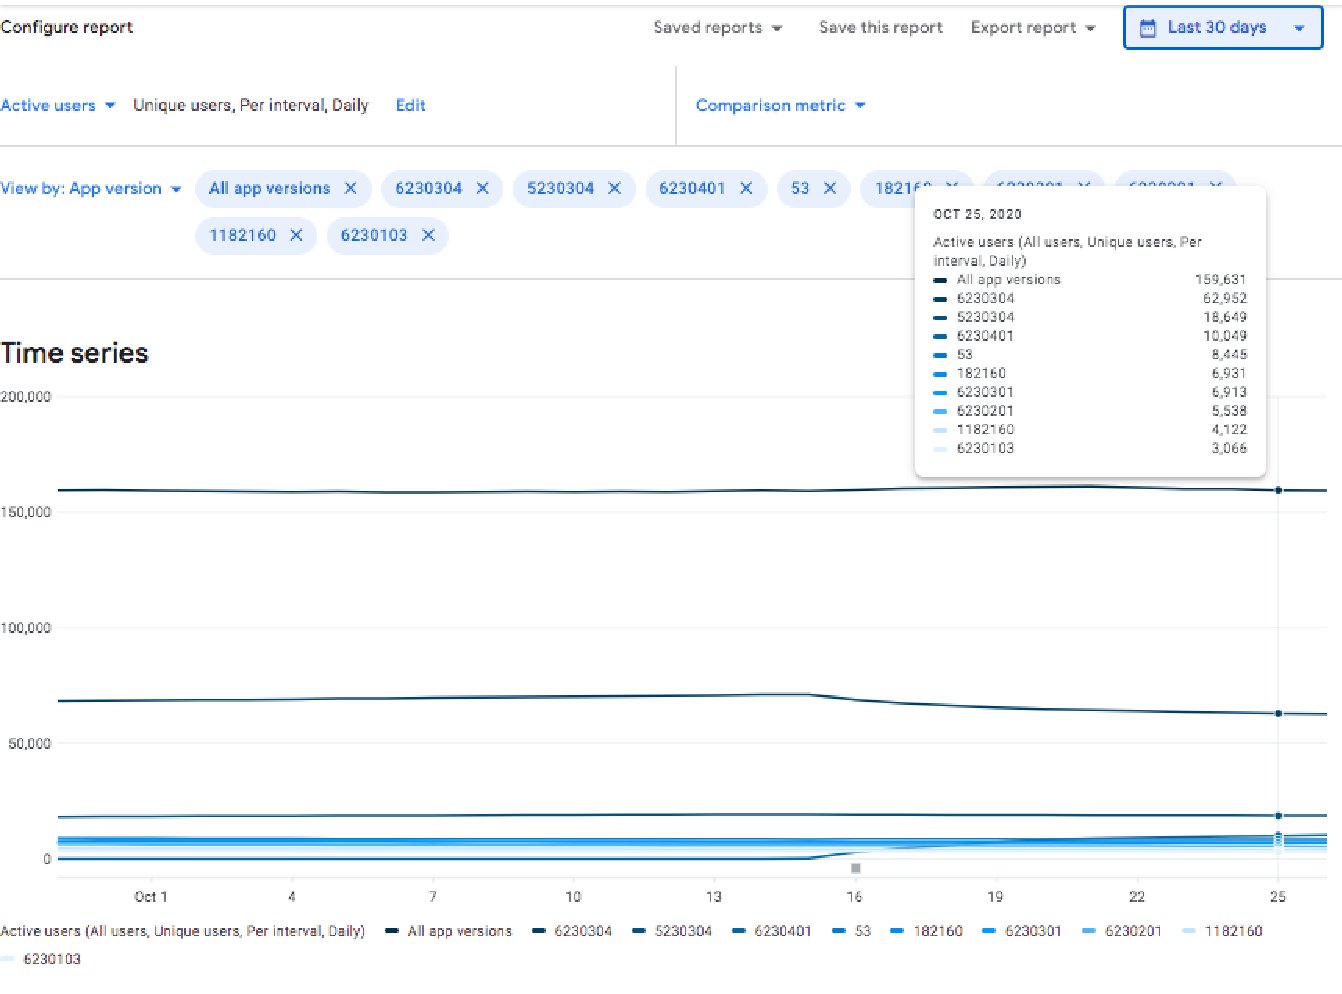
\includegraphics[width=\linewidth]{images/android-vitals-screenshots/kiwix/kiwix-ActiveUsers-30-days-2020-10-29.pdf}
    \caption{Kiwix Android Active Users 30 days by app version}
    \label{fig:kiwix-30d-active-users}
\end{figure*}

As mentioned above, there are various practical constraints to the frequency of releasing mobile apps using an app store. Chiefly there are two constraints: 1) the relatively slow rollout of new releases to the user-base which can take a week or more to achieve 50\% and also 2) the app store's review process which has been a hotly debated topic particularly by developers who may end up waiting days or even weeks for a release to be approved. Apple states~\emph{``Review times may vary by app. On average, 50\% of apps are reviewed in 24 hours and over 90\% are reviewed in 48 hours."} and Google informs developers in Google Play Console~\emph{``We're experiencing longer than usual review times
Due to adjusted work schedules at this time, you may experience longer than usual review times for your app."} ~\sidenote{This message is on the \texttt{app-dashboard} page for each app in Google Play Console and only visible to authorised development team members}. Sophisticated development teams may find ways to alleviate these constraints, for instance by shipping code updates that are applied by a current release rather than by creating and releasing a new binary of the entire app.

Given the constraints that are faced by the vast majority of mobile app developers, of rollouts taking many days and of needing to cope with sometimes lengthy delays in app approvals. 

Mention poor behaviour and their effects on app approvals.

TODO Discuss limits on releasing often that lead to an adapted set of working practices, release frequencies, etc. Perhaps do so elsewhere in this thesis?

\section{Mobile Analytics Usage Lifecycle}~\label{section-mobile-analytics-usage-lifecycle}
For projects that incorporate and use Mobile Analytics, it also has a usage lifecycle. It's important to recognise where the outputs come from, and then how they are interpreted, applied, actioned, and where and how the evidence can be obtained of the effects of applying results of the mobile analytics outputs.

\begin{figure*}
    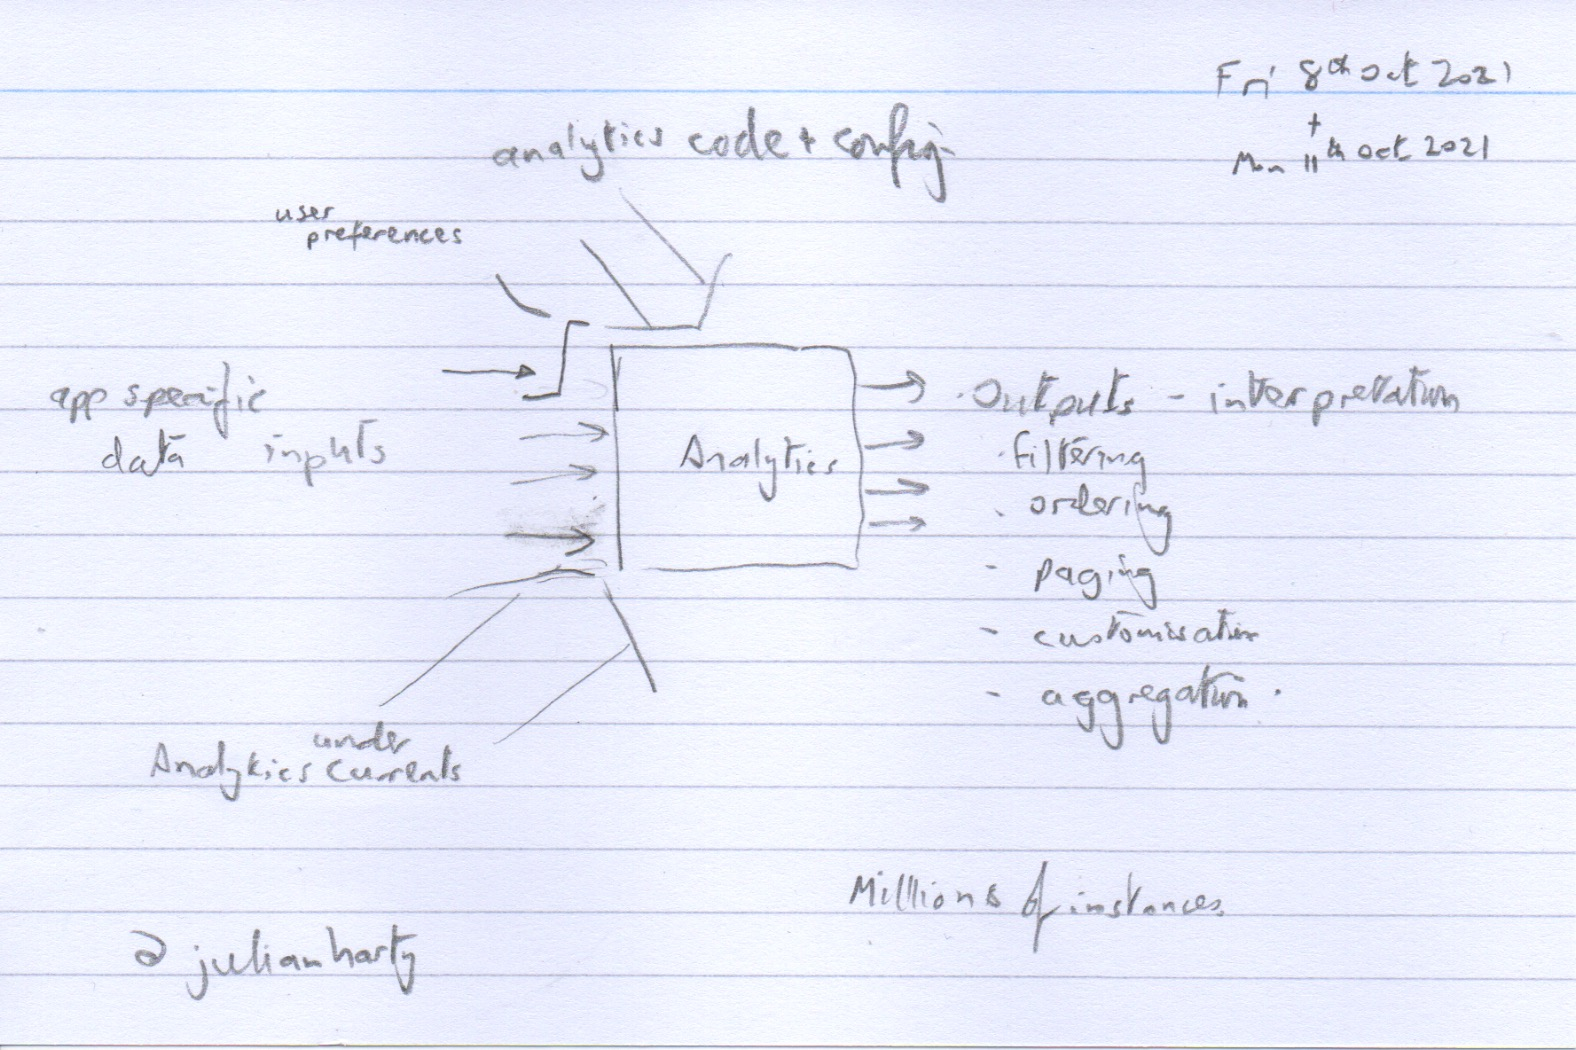
\includegraphics[width=\linewidth]{images/rough-sketches/outputs_from_inputs_code_config-11-oct-2021.jpeg}
    \caption{Outputs from Inputs, Code, and Config (draft)}
    \label{fig:outputs_from_inputs_code_config}
\end{figure*}

Figures \ref{fig:outputs_from_inputs_code_config} and \ref{fig:analytics-feedback-cycle} are connected and illustrate firstly what may affect the outputs pertaining to mobile analytics in isolation, and then how the contents of the first figure fit into a larger, holistic feedback cycle. 

\begin{figure*}
    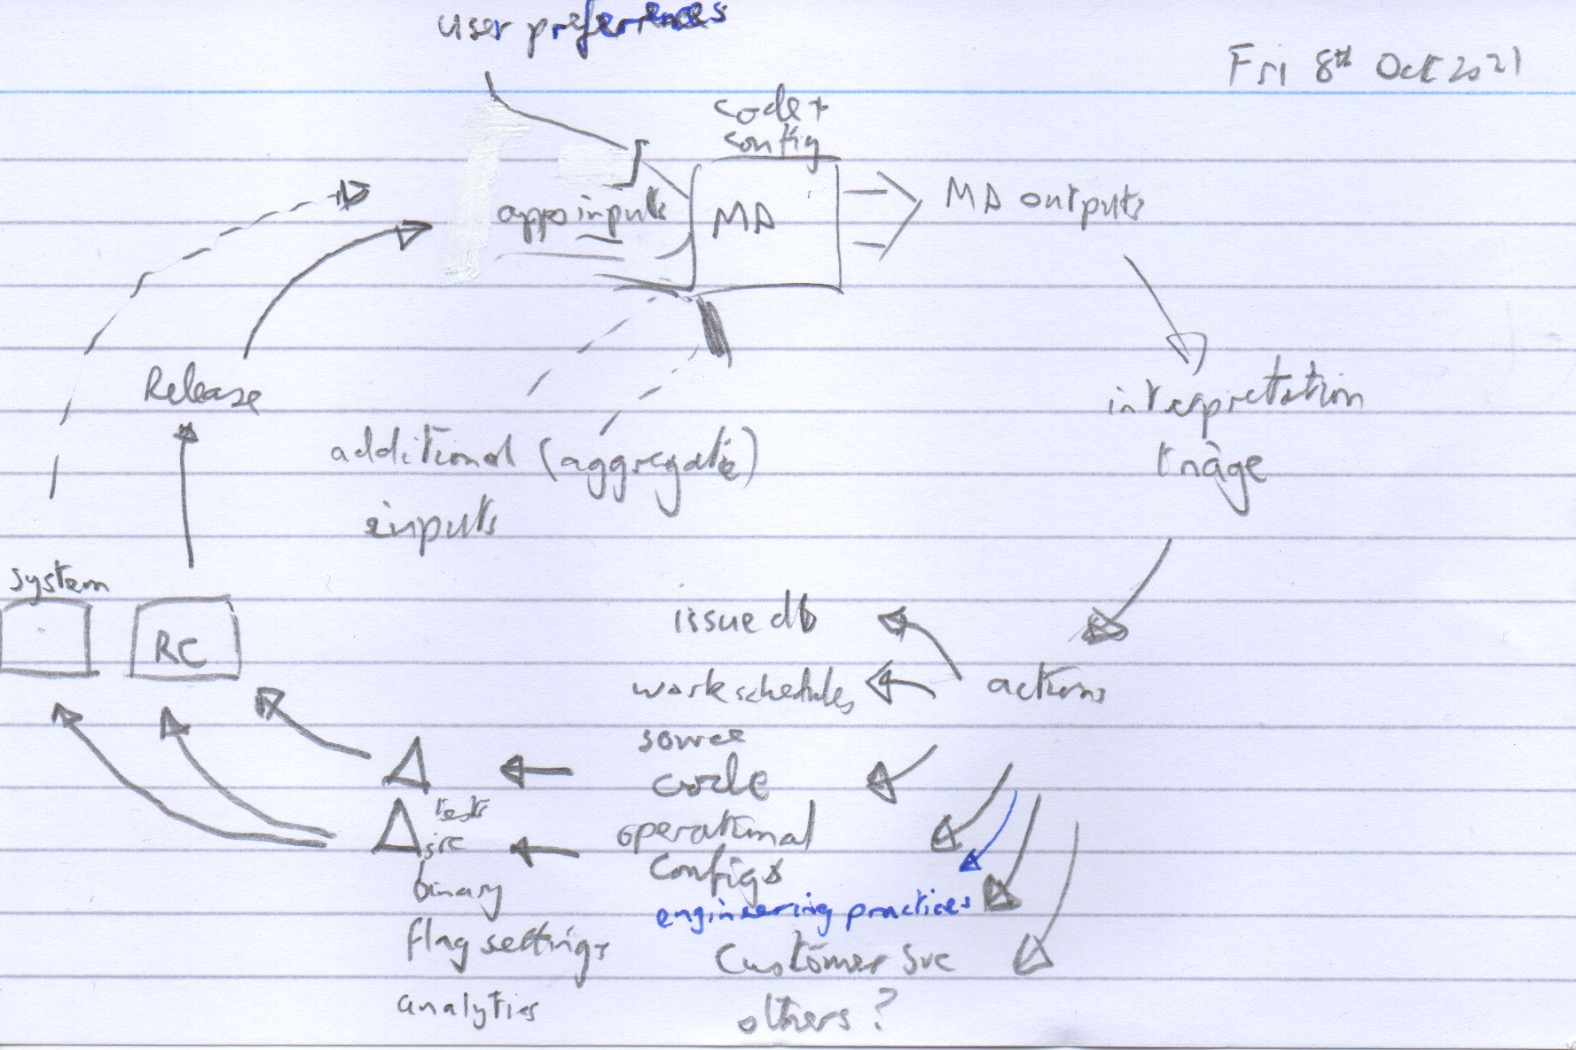
\includegraphics[width=\linewidth]{images/rough-sketches/analytics-feedback-cycle-11-oct-2021.jpeg}
    \caption{Analytics Feedback cycle (draft)}
    \label{fig:analytics-feedback-cycle}
\end{figure*}

In the first of the figures, \ref{fig:outputs_from_inputs_code_config}, working from right to left there is the interpretation of the outputs of a mobile analytics service~\sidenote{The service is provided to developer. It includes the code and configuration that are instantiated to provide analytics processing and reporting aspects; it excludes software running on the mobile devices.}. The interpretation is influenced by the various outputs and how they are used by whoever performs the interpretation. The analytics outputs are influenced by four elements: 
\begin{enumerate}
    \itemsep0em
    \item The service, which includes the instantiation of the server side code and configuration; 
    \item The app-specific inputs (such as failure data e.g. stack traces); 
    \item User-oriented preferences, settings, and so on (e.g. whether analytics reporting is enabled or blocked); and 
    \item Analytics undercurrents (the underlying data and sources may be unavailable to the developers however it may be used by the analytics service, for instance to provide peer-group reports).
\end{enumerate}

The figure illustrates the system for one app, however the analytics service may have as many as millions of instances e.g. Google Play provides one instance of the Google Play Console dashboard for each Android app live in the Play Store. \emph{The instances are unlikely to be identical; they may differ in the analytics code and configuration for instance if Google is running A/B experiments for Google Play Console or performing phased rollouts of new features and/or releases.} Developers may also have customised their analytics service, so they may have distinct views, reports, and interpretations than their co-developers and other colleagues.

In summary, the interpretation of what a mobile analytics service provides depends on the outputs which may, in turn, be affected by their navigation and use. 

The outputs are driven through a combination of elements; these are mainly outside the direct control of the developer, however the developer may be able to influence them. Examples of how the developer may be able to influence these include:
\begin{itemize}
    \itemsep0em
    \item Analytics code and configuration: the developer may be able to opt-in to early experience programs (EEP's), \emph{etc.} These may include new features, reports, and so on that are not available to developers who are not part of these EEP's.
    \item User preferences: the app may include facilities and/or guides aimed at encouraging the user to opt-in (or out) of providing analytics data.
    \item App-specific data inputs - here are some representative examples: the developer may be able to add additional calls to a suitable Mobile Analytics API, or to generate logging messages that are interpreted as failures by the mobile analytics client-side processing. Some Mobile Analytics APIs also provide programmatic access to discard analytics events at run time.  
    \item Analytics undercurrents: the developer may be able to select the peer applications and/or peer category their app is compared with.
\end{itemize}

As mentioned earlier, \secref{fig:analytics-feedback-cycle} subsumes \secref{fig:outputs_from_inputs_code_config} in the upper, central and right areas. Interpretation of the mobile analytics outputs is the first stage in being able to act on them. Triage is the next, and for those deemed sufficiently pertinent are likely to lead to actions. These actions may play out in one or more theatres, for instance in an issues database, in work schedules, in source code, operational configurations, and/or in engineering practices. They may also lead to actions in customer service, and others (such as user-oriented material \emph{e.g.} in online FAQs).

The actions may also result in changes to the sources for the mobile apps and/or in systems that support the app. Changes in the mobile app may form part of a Release Candidate (RC in the diagram) and subsequently in a release. If the release is deployed and then used it will provide fresh app-specific data inputs, and these then feed the mobile analytics.

\begin{figure*}
\RawFloats
\centering
\begin{minipage}{.70\textwidth}
  \centering
  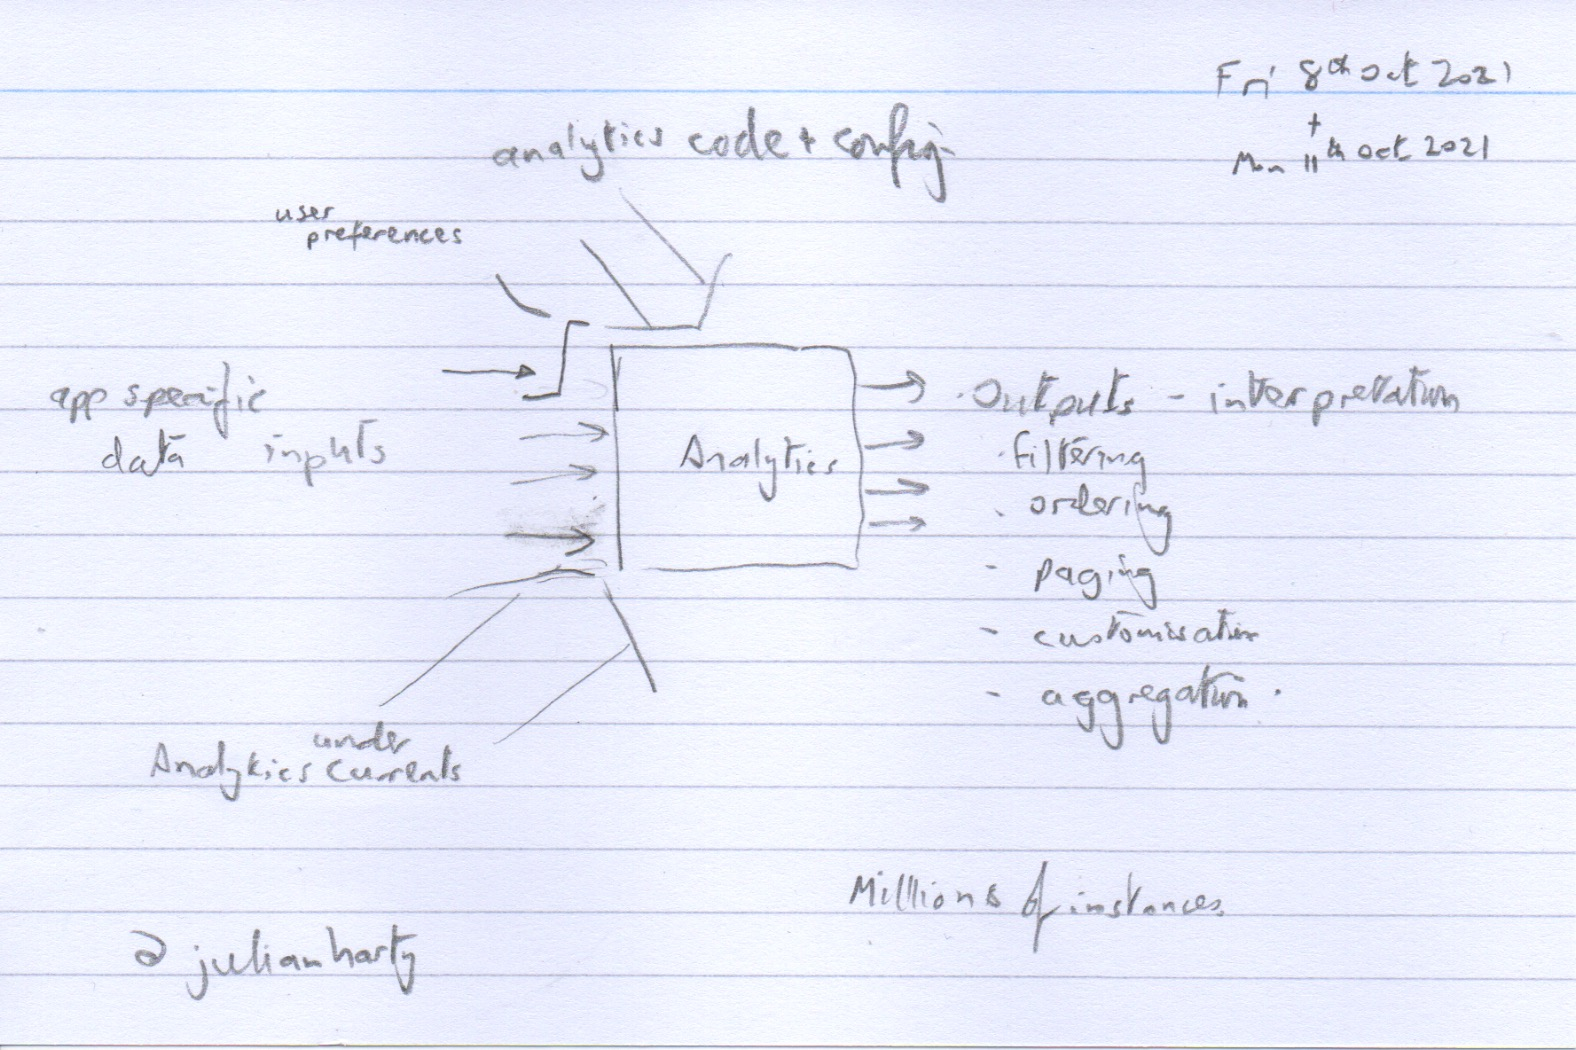
\includegraphics[width=\linewidth]{images/rough-sketches/outputs_from_inputs_code_config-11-oct-2021.jpeg}
  \captionof*{figure}{Outputs from Inputs, Code, and Config (draft)}
\end{minipage}\hfill%
\begin{minipage}{.70\textwidth}
  \centering
  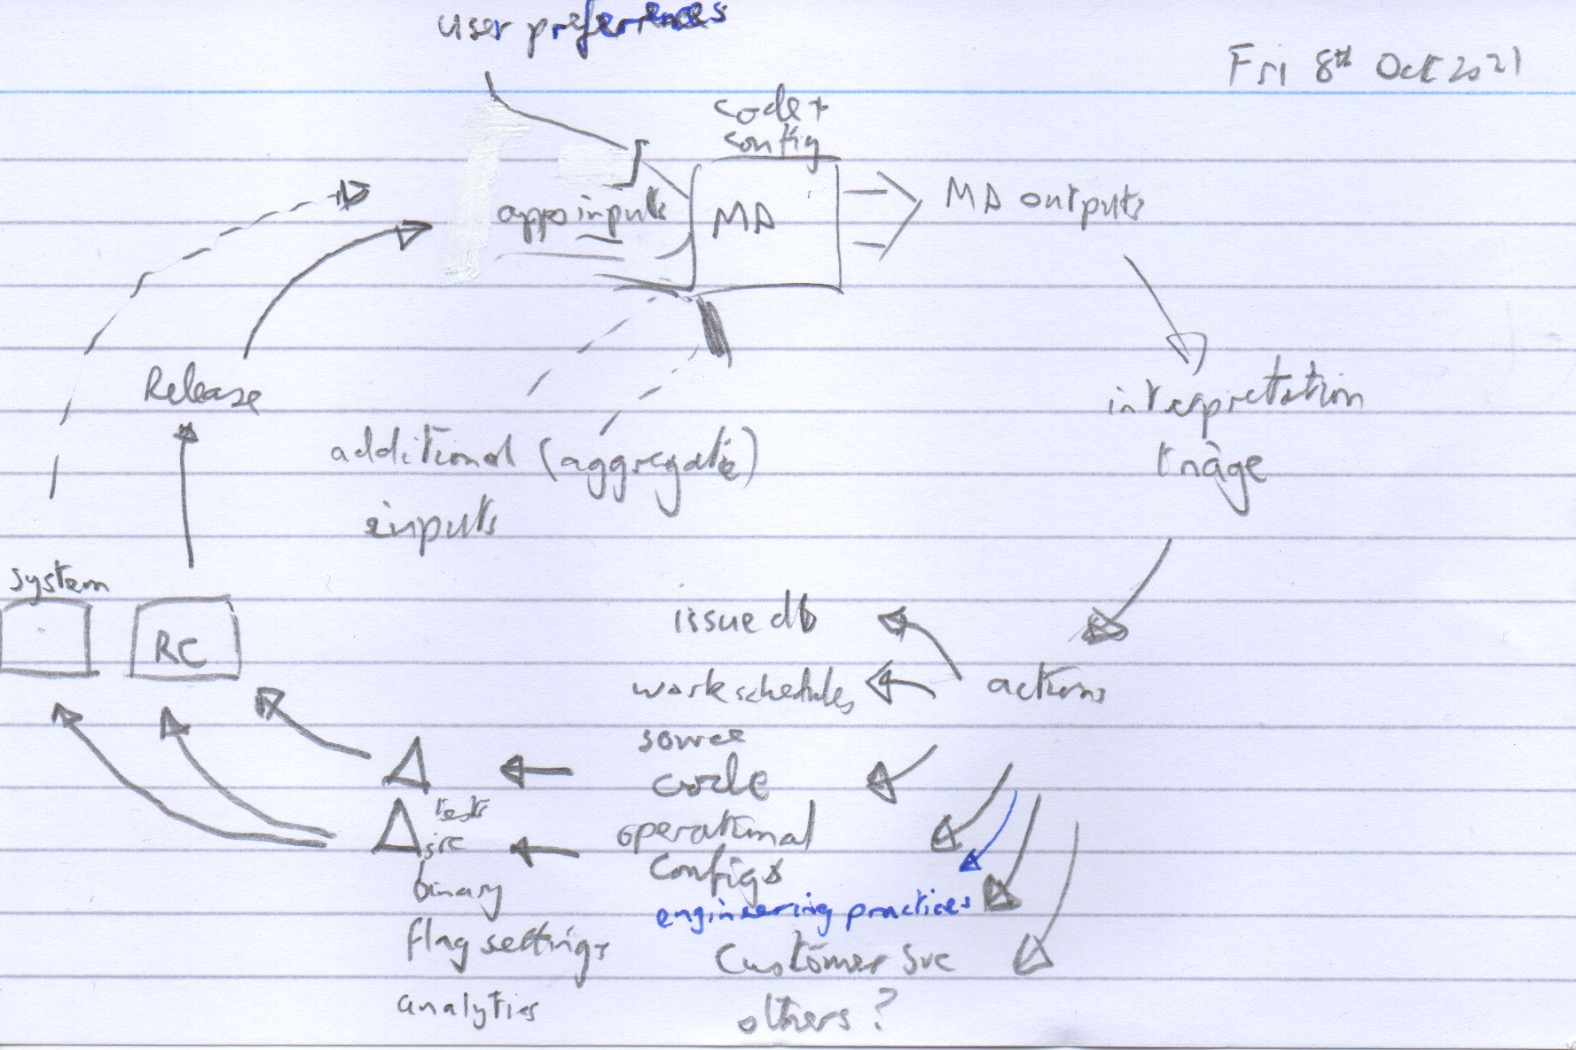
\includegraphics[width=\linewidth]{images/rough-sketches/analytics-feedback-cycle-11-oct-2021.jpeg}
  \captionof*{figure}{Analytics Feedback cycle (draft)}
\end{minipage}
    \caption{Mobile Analytics Contexts}
    \label{fig:mobile-analytics-contexts}
\end{figure*}


FYI: Figure ~\ref{fig:mobile-analytics-contexts} incorporates \secref{fig:outputs_from_inputs_code_config} and \secref{fig:analytics-feedback-cycle} and keeps the two figures together in the document. I've yet to work out if it'll work well with the text, it's here as a reminder I want to improve the links between these two related drawings.



\section{Information sources for app developers}
Developers want and need to know how well their apps are performing from various perspectives such as: growth and adoption (\emph{``do we have more users and are they using the app [more] often?"}), users' ratings and reviews (\emph{``do they like our work?"} and in terms of quality (\emph{``does it perform well? is it fast and reliable?"}). 

\begin{figure*}
    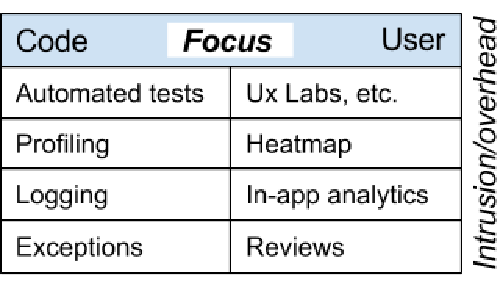
\includegraphics[width=\linewidth]{images/ComparingTechniquesRHS.pdf}
    \caption{Comparing Techniques}
    \label{fig:comparing_techniques}
\end{figure*}

\begin{table}
\RawFloats
    \parbox{.40\linewidth}{
        \centering
        \small
        \begin{tabular}{lll}
            Technique  & Gen. Effort & Usage Effort  \\
            \hline
            Automated Tests  & High  & Medium \\ 
            Profiling   & 1 & 1 \\
            Code Quality tools & 1 & 1 \\
            Logging   & 1 & 1 \\ 
            Exceptions  & 1 & 1 \\ 

        \end{tabular}
        \caption{Focus: Code \label{HRVtable}}
    }
    \hfill
    \parbox{.40\linewidth}{
        \centering
        \small
        \begin{tabular}{ll}
            Technique & vector$_1$  \\
            \hline
            UX labs, etc. & 1  \\ 
            Heatmap & 1  \\ 
            In-app feedback & 1  \\ 
            App-store reviews & 1  \\
        \end{tabular}
        \caption{Focus: User \label{BACtable}}}
    \caption{Comparing techniques}
\end{table}

HRV data in Table \ref{HRVtable} and BAC data in Table \ref{BACtable}.

There are various techniques that can be used to assess aspects of quality of mobile apps. Figure \ref{fig:comparing_techniques} provides a visual overview of eight techniques. Of these four are code-oriented and the remaining four more user- or usage- oriented. They are ordered in approximate rank of the overhead, effort, or intrusion involved of each technique. % MUST-DO continue and expand this argument. Discuss why exceptions were chosen as one of the core elements of this research and PhD thesis.

Google's Google Play app store provides developers with answers to all these niggling questions through a developer-oriented user interface called Google Play Console. 
In Google Play Console they provide various tools, reports and data all aimed at informing developers about how their apps are 'doing' and performing. Broadly, these include an overview page with one line of pre-selected data per app managed by the Google Play \textit{Developer Account}. Then, per app, Google provides an overview dashboard of graphs which, in turn, link to more detailed reports and information which provide greater depth. (Examples are provided in the~\href{appendix-analytics-tools}{\emph{\nameref{appendix-analytics-tools}}} appendix.)  Some graphs only appear when Google's algorithms decide they are relevant, these seem to be related to events and/or volumes of underlying data.




\section{Passive, tacit, and explicit analytics choices}
Various degrees of choices are available depending on how actively the development team wishes to incorporate analytics into their development practices. These include using what already exists, where the data is gathered by others and made available to the developers, here these sources are called \emph{passive analytics}. Developers can choose to take more authority in the data collection, for instance by deciding what data they would like to collect and how they wish to collect it. They can use these tools at various depths, ranging from superficial use to actively maximising the efficacy of using analytics to provide them with the data they believe they need to achieve their outcomes. There is an interesting discussion in a blog article~\sidecite{mukherjee_implicit_versus_explicit_event_tracking_hits_and_misses} on what they term \emph{implicit, or codeless} and \emph{explicit or code-based} event tracking using web analytics tools. The article compares the benefits (hits) and flaws (misses) of both approaches. It also provides a flow chart to help teams select analytics tools that suit their context.

% More reading
% https://web.archive.org/web/20120401053907/http://www.wiikno.com/blog/explicit-vs-implicit-data
% MUST-DO check Patrick's recording of this webinar: https://snowplowanalytics.com/events/explicit-vs-implicit-tracking/ and write up germane items here.


\subsection{Passive Analytics}~\label{subsection-passive-analytics}
Passive analytics are those not actively under the control or influence of the development team, they are provided from other sources such as the operating system or the app store. In the context of this research the passive analytics are all managed by the app store, Google Play, and made available to developers through Google Play Console. As Google states in a US patent,~\emph{``several services provide passive analytics collection such as receiving information about the device type, time of usage, location usage, feature usage, and event reporting."}~\sidecite{googlepatent_hyman2016_collecting_application_usage_analytics}.  

% COULD-DO compare with the concept of passive monitoring https://en.wikipedia.org/wiki/Passive_monitoring however the Wikipedia article doesn't currently add enough to justify citing it or comparing with it.

\subsection{Tacit Analytics}~\label{subsection-tacit-analytics}
Tacit is variously defined as \emph{``Something tacit is implied or understood without question."}~\sidenote{\url{https://www.vocabulary.com/dictionary/tacit}}, \emph{``Understood or implied without being stated."}~\sidenote{\url{https://www.lexico.com/en/definition/tacit}, Note: Lexico.com is a new collaboration between Dictionary.com and Oxford University Press~\url{https://www.lexico.com/about}}, silent, wordless, or noiseless. 
%
It may be something that is inherent in the nature of using many of the third-party analytics libraries. In this research~\emph{tacit analytics} is where developers accept whatever default data is collected by an analytics library without the developer needing to do anything more than integrate the library into their app. 

\subsection{Explicit Analytics}~\label{subsection-explicit-analytics}
Explicit analytics is where developers have actively added code to interact with analytics libraries, for instance by calling methods in the API(s) provided by the library's. There are various degrees of use of the APIs and developers may have various intentions for calling these APIs.

\section{Drilling down into analytics}\label{section-drilling-down-into-analytics}
At the highest level of information, an item and an associated number provides some information: a total crash rate of 99.1 \%, 97K total installs, 37 reviews, and so on. These values may change over time, however if we do not keep track of previous values they cannot be compared, and also relevant information may be hidden behind the totals. The total sums up as many values as exist (from zero values onwards). Some of the reported analytics are of this high-level form.

Totals for subsets of the overall volume of data helps provide additional and potentially relevant information. Relevant subsets for mobile analytics include: date ranges, app releases, platform versions, and many others. Other examples, found in some analytics tools include crash clusters - collections of crash reports considered to be sufficiently similar to enable various individual crashes to be grouped and aggregated. The ability to segment and report on segments allows more detailed analysis than simply observing subsets. 

Comparisons with one or more peer groups provide relational analytics, helping answer: ``how is this app performing compared to various peer groups?" Unless the team has direct access to the data for their peer group, the statistics for the peer group need to be available to a trusted party who perform the comparisons. Some data is publicly available for instance the overall rating of an app together with a limited number of recent reviews and the total installs \textbf{MUST-DO} write up research that uses these sources in the related works chapter, add some of the citations here. There are also commercial services available, and some analytics tools, including Google Play Console, provide these comparisons as part of their services.

Individual records provide the most detail that's available. Note: Developers may be able to create new records and enhance existing records and/or add additional forms of analytics if they want/need more detail. Examples of individual records include stack traces for crashes and similar internal state data for ANRs. Some analytics tools allow developers to capture and subsequently see individual records, for instance details of an item added to an e-commerce shopping cart by an end user. Mobile analytics ultimately can only report on data that is provided to it. 

The analytics tool may or may not make aspects of the data available to the users of the tool. As a concrete example, Google Play Console provides developers access to individual reviews (with their associated rating), it also used to provide access to crashes and ANRs for several years before removing these and replacing them with summary data in 2018 \textbf{MUST-DO} add reference and cite it.

\textbf{MUST-DO} provide screenshots of category peer groups and custom peer groups. Discuss either here, or in a later chapter, Google's cap on the number of changes to the custom peer group.

Two key points in summary: being able to keep track of analytics as they change over time allows comparisons and trends to be determined. Additional detail can help identify meaningful differences for instance that a crash rate is much higher than the mean for a particular model of smartphone. 

How much information is needed to be actionable? (Thought: This may be more of a research question...)


\textbf{MUST-DO} introduce my concept of resolution.

\textbf{PERHAPS} introduce the concept of app peer groups here?


\section{Summary and transition}
% This chapter has introduced various concepts and topics which help provide context for the rest of this thesis. Some additional background material is available in various appendices, including more information on mobile analytics and various software contributions.
We now have a grounding in the domain of mobile apps, logging and mobile analytics which is underpinned by research in both academic research and grey literature. The next chapter describes the application of mobile analytics to software development practices for mobile apps.
\setkeys{Gin}{draft=false}
%\setchapterpreamble[u]{\margintoc}
\chapter{Related Work}
\label{chapter-related-work}
\epigraph{I recall seeing a package to make quotes}{Snowball} % https://tex.stackexchange.com/a/53378/88466

% Additional, older material is online in https://docs.google.com/document/d/1OdoBsLboTZHzv1UP9g7nUriVLgpu6ZGqjXLmRAAlAfs/edit?usp=sharing
% New ideas and material are being added to a Google Doc for a while, then I'll revise this chapter. https://docs.google.com/document/d/1i3cCk2-8zwVioAuMbBQDLcUViihhHY6gk0MJNPevFbA/edit?usp=sharing

\begin{figure}
    \centering
    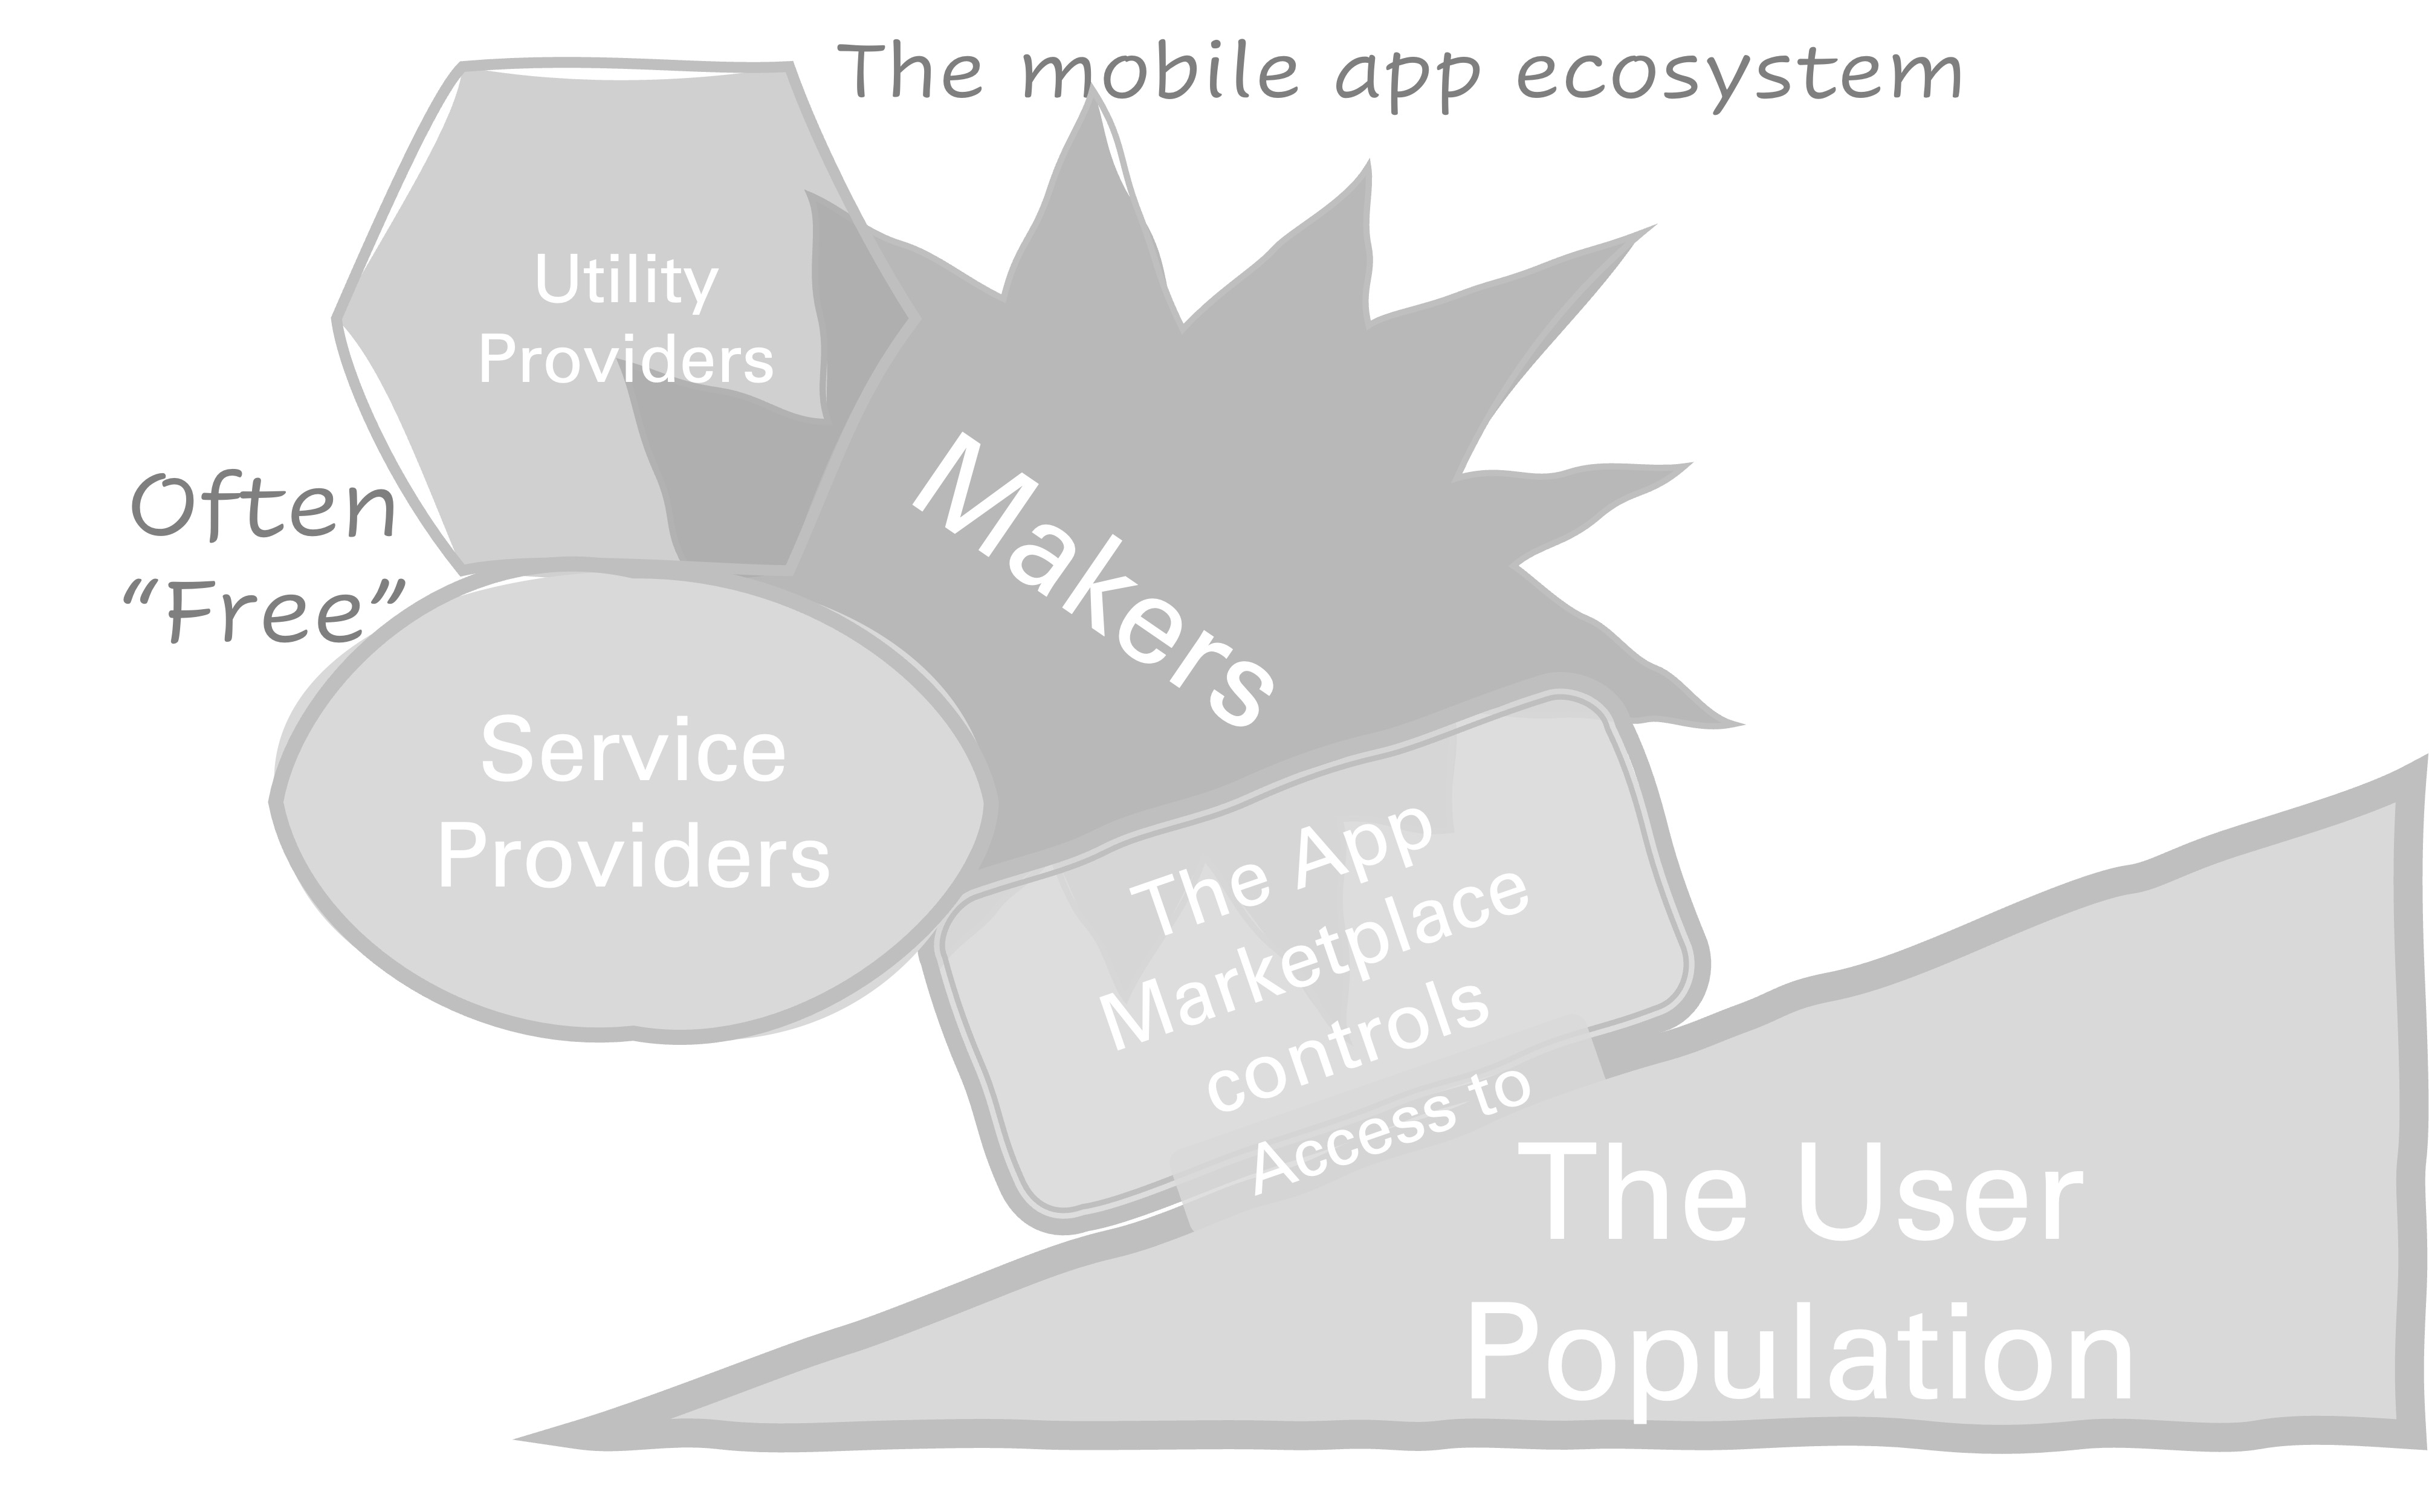
\includegraphics[width=\linewidth]{images/my/the-mobile-app-ecosystem-27-jul-2022.jpg}
    \caption{The Modern Mobile App Ecosystem}
    \label{fig:my_modern-mobile-app-ecosystem}
\end{figure}

The modern mobile ecosystem, illustrated in Figure~\ref{fig:my_modern-mobile-app-ecosystem}, 
sets the context for the thesis and this chapter together with the research questions. The marketplace - the app store - establishes the ecosystem which generates revenues from the user population and frequently to a lesser extent from the makers -  the developers of the apps. Various providers of utilities and services offer these to the makers and they may also obtain revenues from one or more parties that are part of the ecosystem and/or from others, including advertisers.

My work nestles within the works of many people in various related fields: in software quality, in analytics, and in the mobile device ecosystem. As researchers we understand and recognise there are gaps in the current state of the art, this chapter aims to identify several pertinent gaps which led to this research being performed, \emph{i.e.} which motivated me to act. The mobile ecosystems touch on billions of people's lives, where flaws in the apps and the ecosystem can adversely affect the lives of many of those people. 

Research in how mobile apps are created and tested, the relevance of app stores, service and utility providers, the user bases for mobile apps within the overall population of users of an app store ecosystem are all relevant. And meanwhile understanding why it's hard to create reliable software is also vital as part of acknowledging some of the grim realities development teams need to face if they are to succeed in their other goals and objectives for their mobile apps. An understanding of research into how to measure software qualities, and stability in particular, is key to establishing ways mobile analytics measures these qualities. 

At times this chapter will draw from broader sources, for instance in software development, testing, and analytics as these provide context for the particulars of the mobile app ecosystem. Conversely, in my view, and based on discussions at a peer workshop in Japan~\sidecite{nii_shonan_workshop_152}, I proposed a model, shown in Figure~\ref{fig:my_shonan_hysteresis_sketch}, that seemed to be well accepted and became part of the formal post-workshop report~\sidecite{nii_shonan_152_workshop_report}, where the mobile ecosystem is influencing the desktop app ecosystems. Examples include: app stores, per user licensing across multiple devices, public ratings and reviews, platform (device) level, crash reporting, and usage analytics, and so on.

\begin{figure}
    \centering
    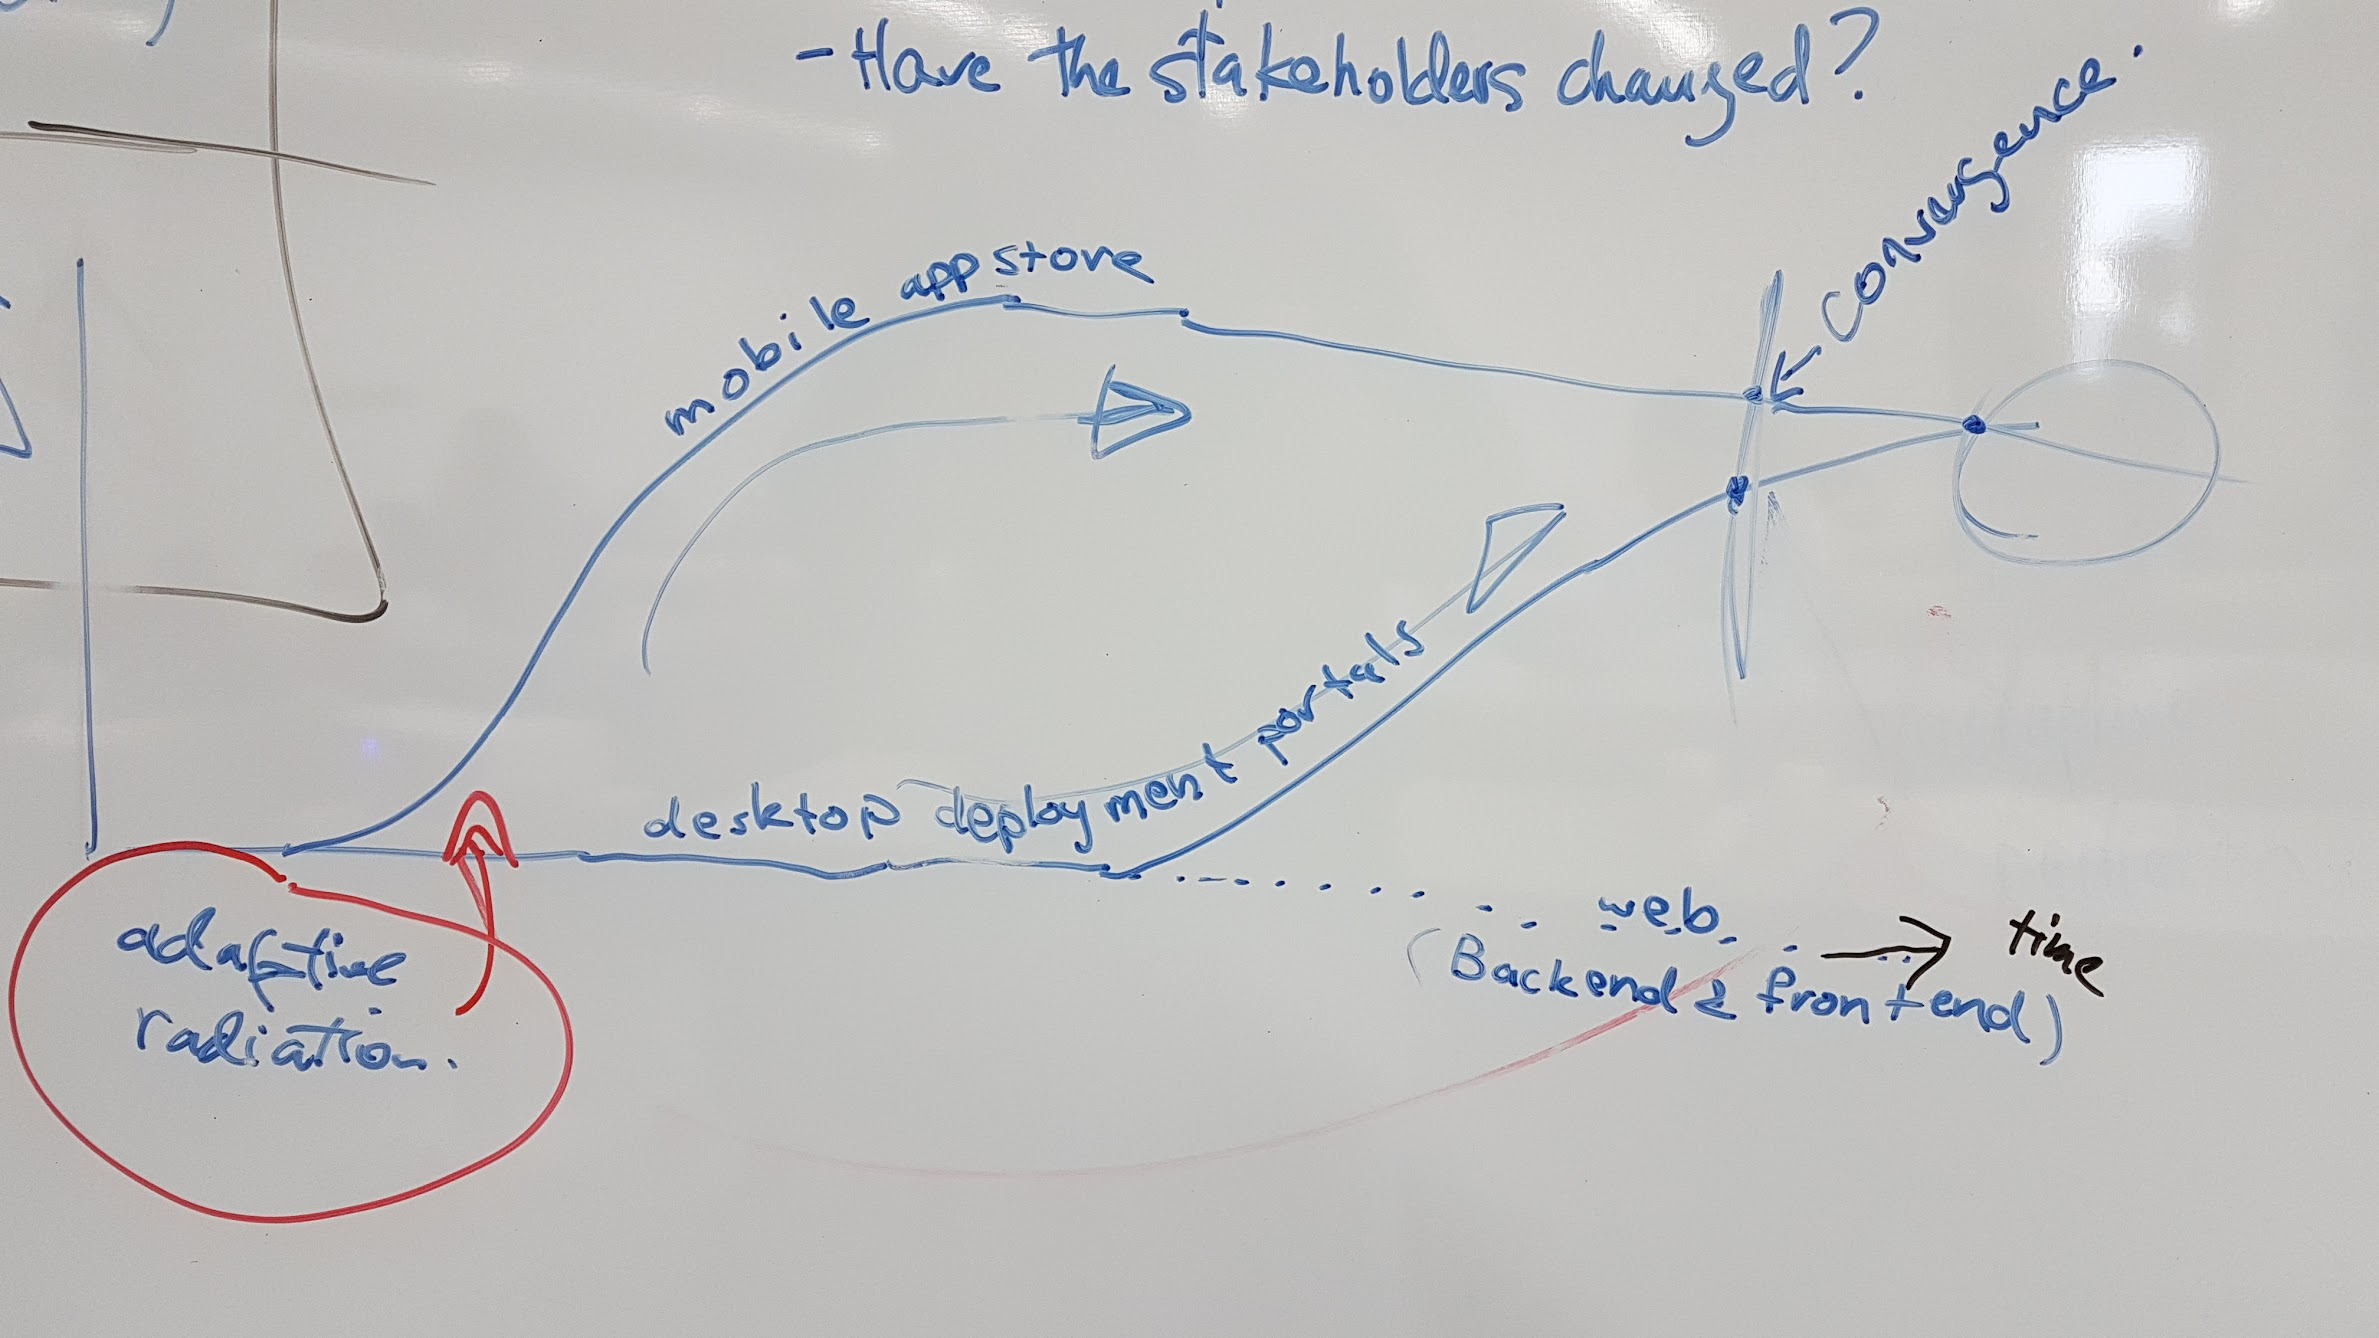
\includegraphics[width=\linewidth]{images/nii-shonan-workshop-152/shonan_hysteresis_diagram_20191210_132528.jpg}
    \caption{Mobile and Desktop Growth and Convergence}
    \label{fig:my_shonan_hysteresis_sketch}
\end{figure}

If the mobile ecosystem is influencing other ecosystems, perhaps this research will also apply to those ecosystems, albeit there are likely to be many distinctions as each ecosystem is distinct and unique.

\newthought{A note on the choice of ecosystem}: 
The practicalities of the research and the case studies where nearly all the work pertains to the Google Android ecosystem also helps in the selection criteria of relevant related works. As the vast majority of active research in the domain of mobile apps also pertains to this ecosystem, this means the topic is richly served in terms of related works.

\newthought{Contents of this chapter}:
The next section provides an overview of the methodology for this chapter, this may be removed pre-submission, nonetheless it is intended to help explain the rationale and the method that underpins the research into related work.

Subsequent sections are organised to provide the context of the research. There are two strands of existing research that this research builds on The first strand comes from software development generally in terms of: development practices, software quality, including measuring software quality, and then the use of software analytics. The second strand is the app store ecosystem and the effects it places on software development and engineering.

These two strands both affect development practices when developing, testing, releasing, and maintaining mobile apps. A particular aspect of developing mobile apps - feedback - is further developed in terms of the feedback that's available to app developers and the research into several of these forms of feedback. The final topic is existing research into crashes and freezes of mobile apps - these are both indicators of poor quality-in-use of the mobile app.

\begin{figure}
    \centering
    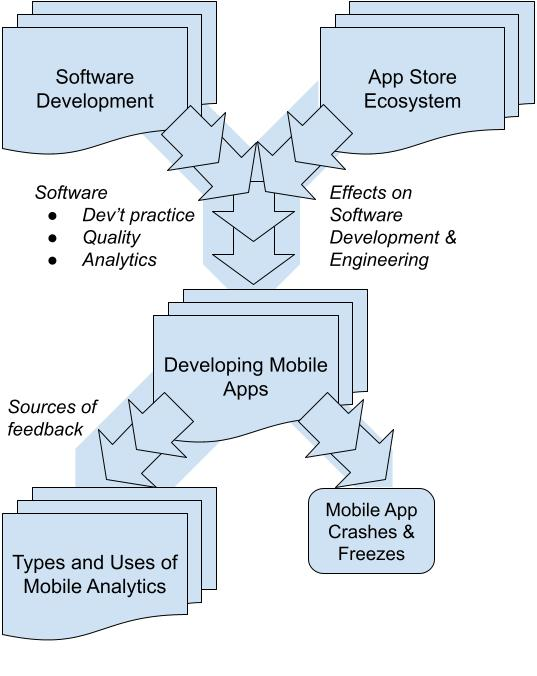
\includegraphics[width=\textwidth]{images/my/related-work-chapter-structure-27-jul-2022b.jpeg}
    \caption{Structure of this related work chapter\\ Source: \href{https://docs.google.com/drawings/d/1DosM__BfTGqoIYkkkltbyDreCT5wYC1Z0mR9i1ZSxWc/edit?usp=sharing}{Google Drawing}, access limited to collaborators to this thesis.}
    \label{fig:related-work-chapter-structure}
\end{figure}

% Reinstate the following once I've completed the first complete draft of the following sections.
% starting with research into app stores and their effects on software development and engineering \ref{rw-app-stores-and-their-effects-on-software-development-and-engineering}...

\section*{Notes on the proposed tactics and topics for the related work chapter}
Marian suggests I aim for writing brief, one-paragraph summaries and apply the T tactic of the broad literature, the top bar of the T are the many and various papers on a topic, and I'm picking these ones that are most directly germane to my research which become the vertical bar of the T.\pending{I'm still currently more verbose than this :(} 

Marian also suggested I might end up with two or a maximum of 3 levels of Ts. The higher level would be on Software Quality Improvement. The lower level would be on mobile analytics.

Where others have done similar work they've done so in other ways eg MSR rather than focusing on the development teams. When I observed the teams the effects of the processes, artefacts, and the tools emerged. This is why I've picked these 3 aspects and 6 perspectives. 

\subsection*{Some notes on the methods used for the literature review}

\begin{figure}
    \centering
    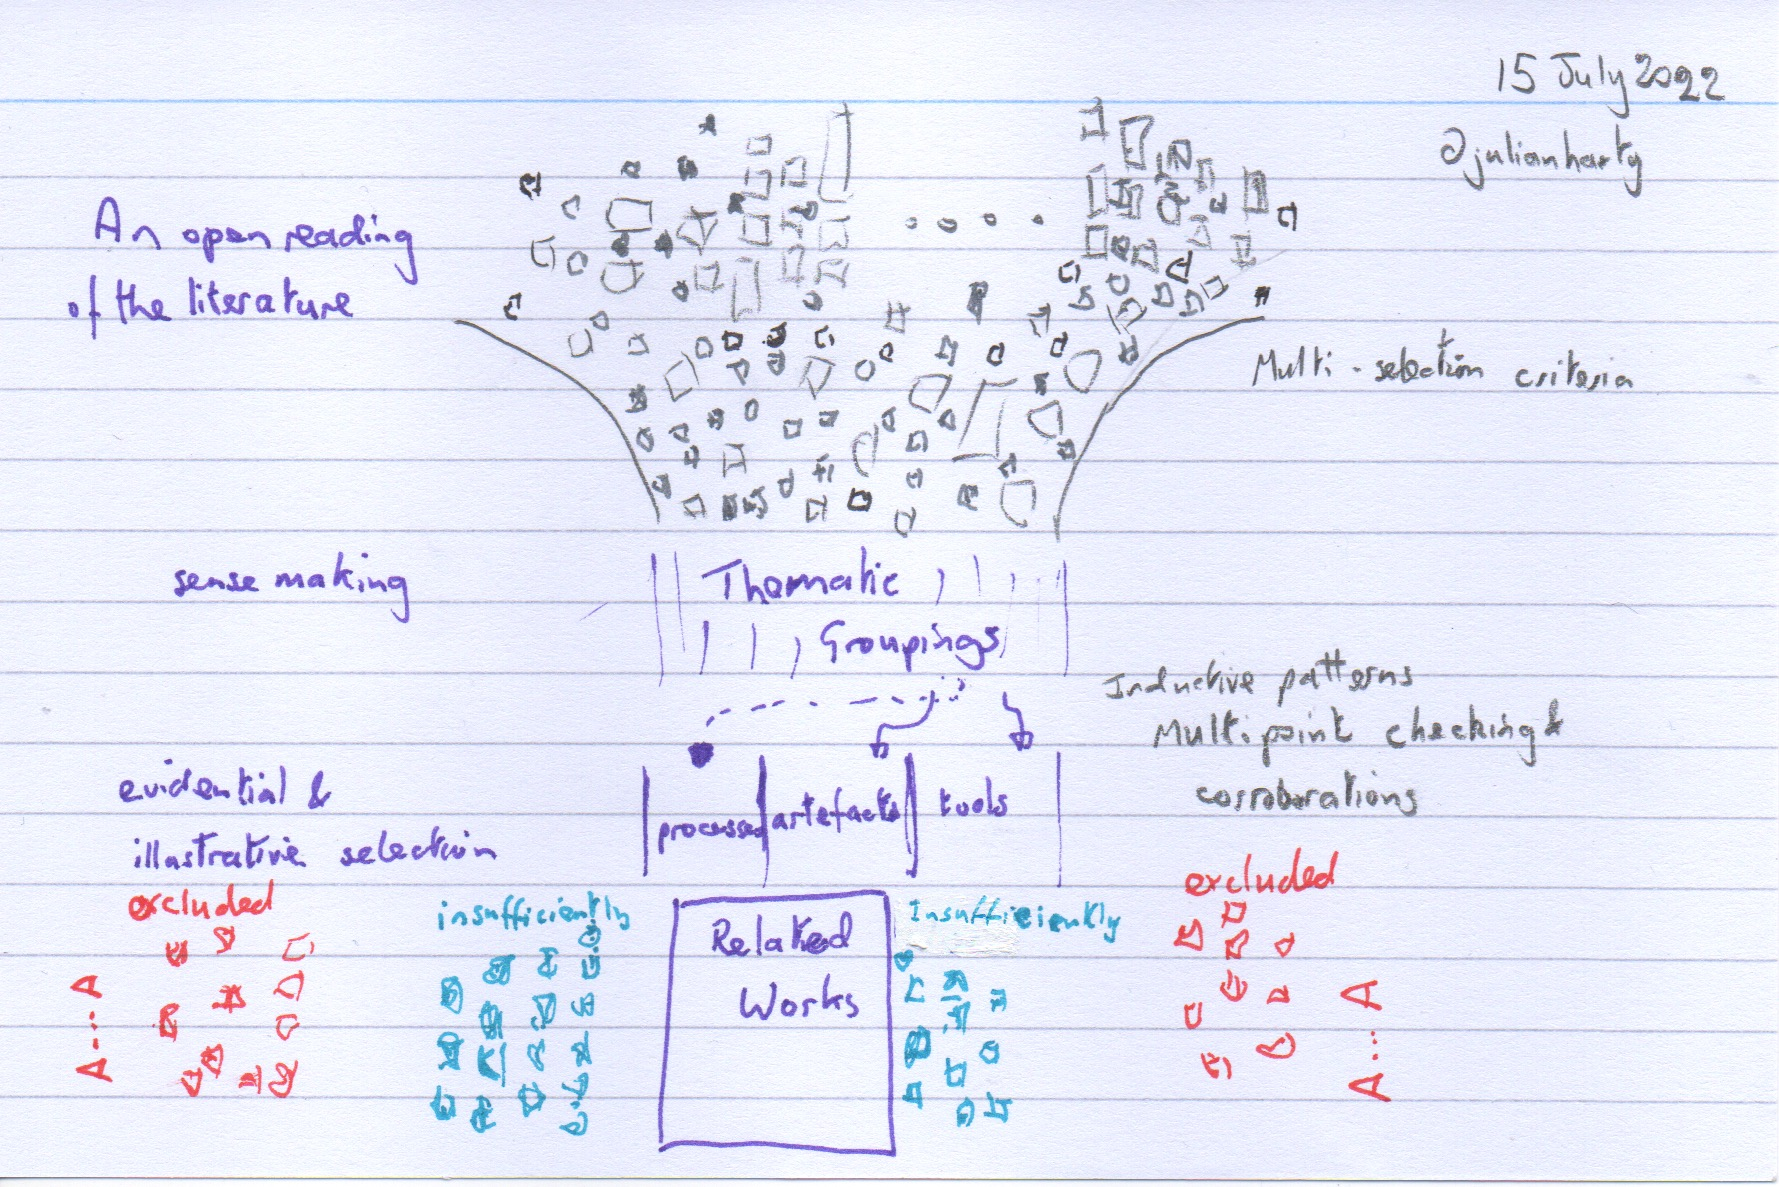
\includegraphics[width=\textwidth]{images/rough-sketches/literature-review-overview.jpeg}
    \caption{Overview of the literature review process and outcomes}
    \label{fig:literature-review-overview}
\end{figure}

Figure \ref{fig:literature-review-overview} illustrates my approach to researching prior work in the use of mobile analytics by app developers in order to measure and improve the stability/reliability of their mobile apps in the field/in the wild. Various searches, including keyword, tags, and related items, were incorporated into the searches. Initial sources included Google Scholar to find the more research oriented materials and Google Search particularly for grey materials, helped provide initial material to seed further searches. Specialist search tools were used where sites provided them, for instance on stack exchange sites such as StackOverflow, GitHub.com, acm.org, ieee.org, and medium.com their respective search engines were used frequently. Where practical copies of material has been preserved privately and backed up using at least one commercial, paid-for, cloud file storage service.

Multi-selection criteria are used to select material that appears of interest, relevant, and plausible. Generally bibliographic entries were obtained and these where checked for accuracy and completeness. Grey material seldom has a bibliographic entry, these were created, generally by hand, and preserved.

Through a process of sense-making, cross-checking, and corroborations various thematic groupings emerged together with potential relationships between the thematic groups. On reflection three clearly distinct and vital aspects emerged in the related work - the development practices used by mobile app developers, the artefacts they create and maintain, and the mobile analytics tools the developers use. These were further refined into six perspectives, using a three-by-two matrix: the x-axis incorporates the three aspects of processes, artefacts, and mobile analytics tools; the y-axis focuses on the current \emph{what is}, and \emph{what might be} in terms of making improvements.\pending{Arosha suggested three pillars which sounds good.}

The research materials and the bibliographic entries are maintained online. The most relevant ones are included in this thesis, many more are maintained in an `outtakes' folder, for example as `fieldstones'~\citep{weinberg2006weinberg} or in an insufficiently-related-works chapter. There's also an `excluded biography' file which helps reduce unnecessary repetition or groundhog day like practices. In the figure (\ref{fig:literature-review-overview}) the two \texttt{A ... A}'s wraps around - excluded works and insufficiently related works are similar distanced to this related works chapter.

In reading the literature various \textit{false friends} emerged, papers that first appear relevant because of their titles and/or abstracts but turn out to be on very different topics. 
Knowing about the concept of false friends and having pragmatic strategies to deal with them is important to avoid misunderstandings or misleading application of their work, 
based on \citep[p. 1833]{chamizodominguez2002_false_friends_their_origins_and_semantics_in_some_languages}. 
\citet{shaw1989_comparing_conceptual_structures__consensus_conflict_correspondence_and_contrast} uses the term 'conflict`, where, \emph{``experts use [the] same terminology for different concepts"}~\citep[p. 3]{shaw1989_comparing_conceptual_structures__consensus_conflict_correspondence_and_contrast} (and, indeed, using their terminology here there is a `correspondence' where experts use two terms to describe the same concept e.g. `false friends' and `conflict' both describe the same concept.). For this research my work was limited to recognising false friends and identifying some examples. 

So somehow I should aim to have the chapter structured with the following topics:\pending{This is a note to myself and needs replacing as I refine the chapter.}
\begin{enumerate}
    \item \textbf{Software Quality [Improvements] for mobile app developers}: Software Quality has been a contested topic for decades with no single accepted coherent agreement on what form(s) it takes, how software quality is measured, etc. Then comes the similarly vexed challenge of determining the concept and application of improvement in the quality/qualities of software. 
    \item \textbf{Mobile Analytics}: Research into \textbf{Processes, artefacts, and tools} necessary when using mobile analytics for improving software quality/qualities. These groupings emerged during the analysis of the literature and through understanding the practices of app developers.
    \begin{itemize}
        \item \textbf{Processes}: a.k.a. Analytics in Use - research into the processes developers use when they use mobile analytics
        \item \textbf{Artefacts}: things the developers create and maintain as part of their development work. Some of these are generated, in particular the app binary that is destined for end users once delivered by the app store.
        \item \textbf{Mobile Analytics Tools}: that the app developers use are worth researching in order to learn about their characteristics.
    \end{itemize}
\end{enumerate}

\subsection*{Software Quality Improvements for mobile app developers}
Here topics might include the measures that have been used by app developers to measure software quality - as confirmed by research literature and grey materials. I suspect this is where I'd include sources of information about software quality (\secref{rw-sources-of-info-on-software-quality-for-devs-of-mobile-apps}).

\subsection*{Development Processes for mobile apps}
Here topics include how the developers are perceived to work when they develop mobile apps, how they spend their time, how they structure and organise their work, etc. I suspect software testing fits here as well as how devs make mobile apps (the artefacts e.g. build scripts would go in the artefacts section).

\subsection*{Artefacts for mobile apps}
There's no end of research on artefacts from various subsets of opensource Android projects. Quite how well these reflect the population of shipping mobile apps (in Google Play in particular) is open to discussion. I can potentially include my joint research on logging practices as we aimed to only analyse projects where the codebase was actively maintained, etc. Research into logging practices by devs might also fit here (however how they use logging would be part of the section on development processes).

\subsection*{Mobile Analytics (and Mobile Analytics tools)}
I think it's germane to include research on the use of mobile analytics and any research into the tools, including the SDKs, data leakage, privacy, etc.

\subsection*{Thoughts on the above organisation of the related works}
As I've written the notes for each of the previous subsections I've had several instances where I've written about a single topic split across processes and artefacts. Perhaps it'd be better to keep the topics together and then summarise the topics by explaining there's a key distinction between the artefacts that exist and how they're used in practice. If so, then the alignment with the six perspectives would occur towards the end of this chapter rather than being used throughout. Let's see.

 % Moved the content to a separate file to reduce noise for the reader of the chapter in latex.


\section{Software Development}
% For the purposes of this research there are at least two camps in research. The first camp is where the research comes from the field and is applied in the field of production, shipping software and the second camp seeks ways to improve the tools, techniques, and results \emph{without} dealing with the practical aspects. The work of the second camp remains unused in reality and oft only reviewed in-passing by other researchers who want to claim their research generates better `results' than that of the other camp members. The second camp's work overall is on an orthogonal path to the work and world of practitioners. The gulf seems wide between these two camps.

%%% Rationale for including this topic 
Mobile apps are developed using similar practices to other modern software projects, however there are key distinctions/differences such as: the build, packaging, and release processes (which are relatively similar to those for software apps generally), how analytics is designed, implemented, and how analytics works all differ. There are also nuances in the effects of software quality as measured by the app store which are important for us to be aware of.

This section, and associated subsections, provide context for the more specific domain of mobile apps, covered in \secref{rw-developing-mobile-apps-section}~\sidenote{As an observation there appears to be little research into desktop apps, such as those available on MacOS. However, research in that area is outside the scope of this research.}.
 
This section covers the following topics: \secref{rw-software-development-practices-topic}, \secref{rw-software-quality-including-measurement-topic}, and \secref{rw-software-analytics-topic}.

\subsection{Software development practices}~\label{rw-software-development-practices-topic}
Jez Humble is a well respected leader in modern software development practices who popularised the concepts of Continuous Delivery and DevOps. In \sidecite{humble2018_continuous_delivery_sounds_great} he argues the benefits of using continuous delivery to reduce risks and transaction costs. to create fast feedback loops, and work in small batches. He also believes it can be applied to any software and any domain. He concludes: \emph{``This, in turn, increases the quality of products, allows developers to react more rapidly to incidents and changing requirements and, in turn, build more stable and higher-quality products and services at lower costs.''}~\sidecite[][p. 39]{humble2018_continuous_delivery_sounds_great}. 

To be successful in applying continuous delivery he identifies the importance of continuous, daily improvement and constant discipline to seek higher performance. Can we assume continuous delivery is suitable for mobile apps and can be applied by developers of those mobile apps? 


\subsection{Software quality, including measuring software quality}~\label{rw-software-quality-including-measurement-topic}

Early work, presented at ICSE in 1997, compared two approaches to software testing - debug testing and operational testing~\sidecite{frankl1997choosing_testing_for_reliability}. Their research considered the two approaches including their efficacy at improving reliability of the software being tested. In their work they challenged the focus on faults which they stated was nebulous and not necessarily the best term to use to describe what happened when failures were detected or when changes were made to 'fix' the code that led to the failures. They introduced the concept or notion of \emph{failure regions}, which could be \emph{``eliminated by a program change''}[p. 70]. Their work and their concepts align well with the use of mobile analytics to identify failures, and failure regions that are detected by mobile analytics and potentially addressed by changes to the program \emph{i.e.} the mobile app. We will revisit this paper in \secref{rw-mobile-app-crashes-topic}.


%Measuring software quality

One of the challenges has been to find ways to measure beyond an app, to behaviours that are externally observable but not easy to measure within an app. Unresponsiveness of software is a particular concern for mobile apps where apps stop responding for longer than deemed acceptable. Google Android coined the term ANR (TODO replace with glossary entry) for when the application stops responding. One of the challenges has been how to detect and measure these, particularly remotely on end-user devices. 

An opensource project provides Android developers with a mechanism to detect and report ANRs in their application. It includes support to report the ANRs to various crash reporters~\cite{salomonbrys_github_anr_watchdog}. (Two of the four listed (Crashlytics and HockeyApp) have been acquired by Google and Microsoft respectively). Note: In 2012, Google was asked to provide a facility to detect ANRs from the application~\footnote{\url{https://issuetracker.google.com/issues/36951741}} so developers would be aware of them and be able to address them. The issue was marked obsolete by Google in 2014 without comment. Approximately six years later, in 2020, Google Android launched an API call that apps can use to determine whether the app was previously quit by the operating system (see \secref{tata-chapter-section-design} for more detail). 

\subsection{Software analytics}~\label{rw-software-analytics-topic}
Software analytics includes the use of analytics to measure and potentially improve processes, products, and software tools. Some of the early published research came from Microsoft Research. For example, Buse and Zimmerman wrote a short paper in 2010 which helped establish the field of:~\emph{``Analytics for Software Development"}~\sidecite{buse_analytics_2010}. The first figure in that paper is reproduced here as~\ref{fig:software_analytics_buse_and_zimmerman_2010}. They had derived that figure from a more general business-focused diagram in Davenport and Harris's book~\emph{``Analytics at work: Smarter decisions, better results"}~\cite{davenport2010analytics_at_work},  in Figure 1.1, titled\emph{``Key questions addressed by analytics"} and found in page 7 of ~\sidecite{davenport2010analytics_at_work}). 

Buse and Zimmermann
\begin{figure}
    \centering
    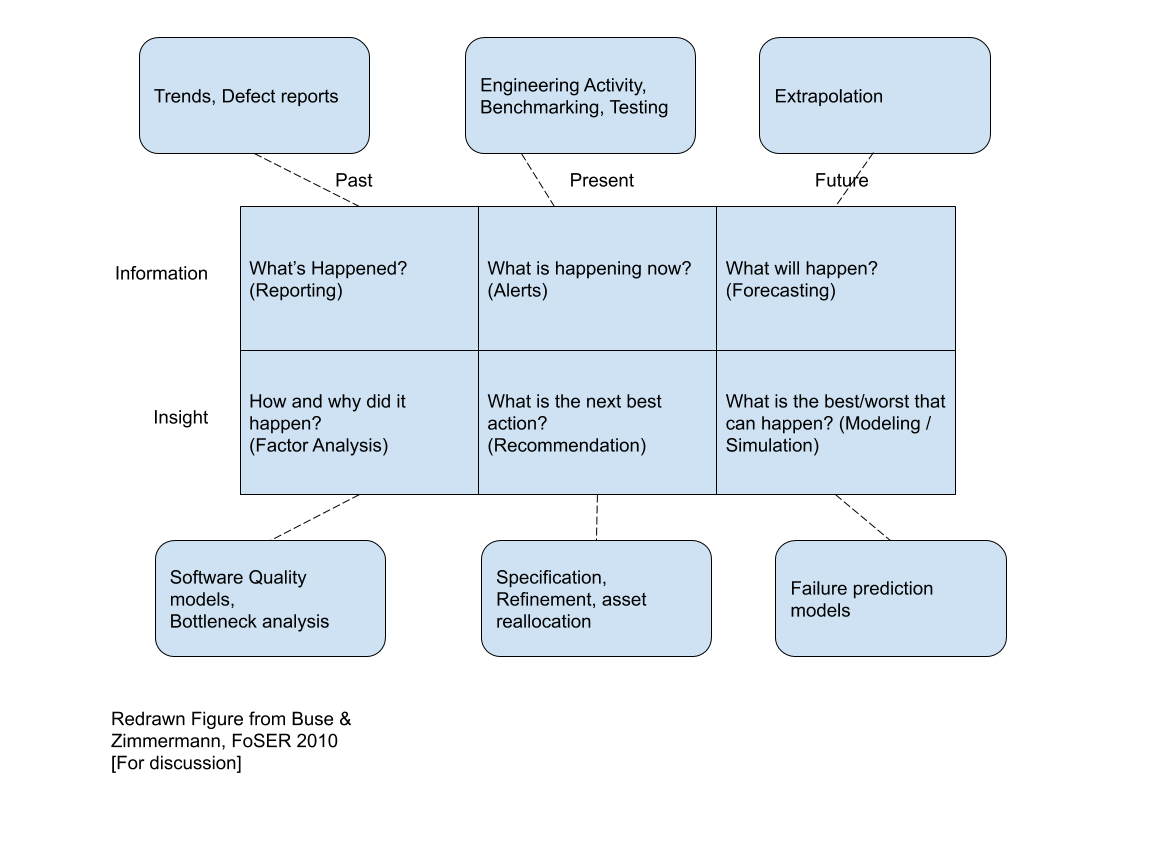
\includegraphics[width=14cm]{images/Buse_and_Zimmermann_2010_figure.png}
    \caption{Software Analytics, Buse and Zimmerman (2010)}
    \label{fig:software_analytics_buse_and_zimmerman_2010}
\end{figure}


In the Buse and Zimmermann paper they \emph{``distinguish between questions of information which can be directly measured, from questions of insight which arise from a careful analytic analysis and provide managers with a basis for action.''}~\cite{buse_analytics_2010}.

\subsubsection{The development managers' perspective}
\emph{``Information needs for software development analytics"}~\cite{buse2012_information_needs_for_software_development_analytics}. They asked 110 Microsofties, a mix of development leads and managers about their use of software development analytics. MUST-DO discuss how my work and their guidelines for software development analytics align. What does my work add to their work? What does it provide that they identified back in 2012? Their focus seems to be more on the code than the product of the code (apps and the services (and the qualities of those services) those apps provide to end users). What information do mobile app developers need in terms of improving the reliability of their apps? How can the developers make good decisions in this area?


\begin{figure}
    \centering
    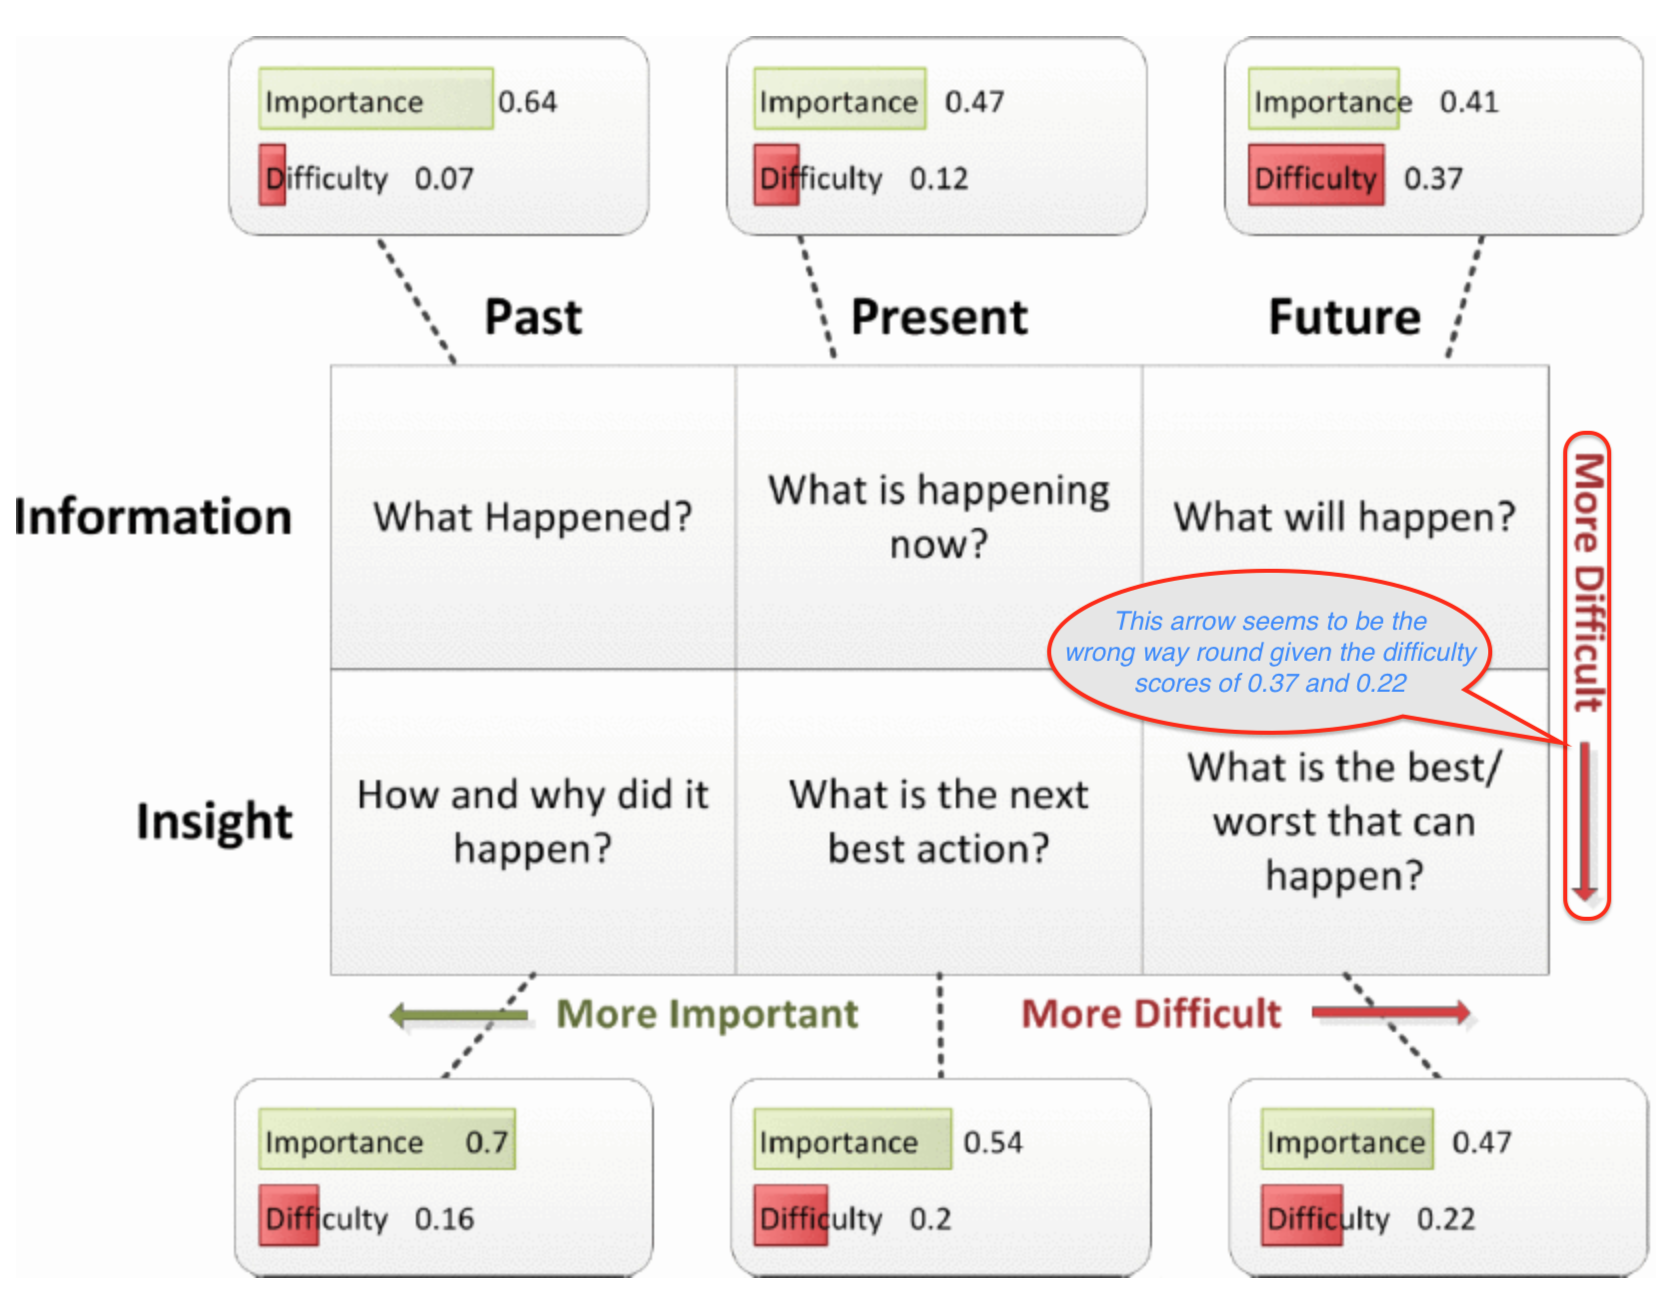
\includegraphics[width=\linewidth]{images/related-work/buse2012-edited-figure-2.png}
    \caption{Revised Figure 2 from TODO}~\footnote{\cite{buse2012_information_needs_for_software_development_analytics}}
    \label{fig:buse2012-edited-figure-2}
\end{figure}


\begin{itemize}
    \item ~\emph{``we ultimately want to} empower software development teams to independently gain and share insight \emph{from their data without relying on a separate entity"}
    \item \emph{``Analytics can help: monitor a project; know what's really working; improve efficiency; manage risk; anticipate changes; evaluate past decisions."}
    
    \item Oddly, Figure 2 in their paper seems to have a mistake in the direction of More Difficult from Information to Insight, see~\ref{fig:buse2012-edited-figure-2}.
    
    \item \emph{``In other words, both developers and managers find it more important to understand the past than try to predict the future; echoing George Santayana, “those who cannot remember the past are condemned to repeat it.”"}.
    
    \item From Figure 4 in their work, Failure Information (\emph{``reports of crashes or other problems"})is in the top 3 that the development leads would use and top for managers when making decisions relevant to their engineering process. Telemetry (\emph{``user benchmarks"} would be used by around 80\% of development leads and 90\% of managers in the survey.
    
    \item \emph{``The landscape of artifacts and indicators in software engineering is well known, but the concrete decisions they might support are not. We conjecture that understanding how managers and developers can make use of information is critical to understanding what information should be delivered to them."}. My research somewhat inverts this by looking at what's being delivered in terms of commercial, pre-existing mobile analytics and considers how that information has been used to improve the reliability of the mobile apps that were the source of the raw information.
    
\end{itemize}~\cite{buse2012_information_needs_for_software_development_analytics}.

\subsubsection{Learning from Windows Error Reporting}~\label{rw-learning-from-wer}
The data collection and analysis of Android Vitals has some similarities with Microsoft's \acrfull{wer}\index{Windows Error Reporting (WER)} which they describe in an article in 2011~\cite{kinshuman2011_debugging_in_the_very_large} and a longer conference paper from 2009~\cite{kinshuman2009_debugging_in_the_very_large}. Similarities include both mechanisms being designed to work effectively at scale of at least a billion end-user machines/devices, capturing crash data, and using error statistics as a tool in debugging. Differences include the platform (Android), the lack of automatic diagnosis (which WER provided), and most relevantly, Google provides several million third-party developers with access to data for the apps they are responsible for and provides them with various comparative analytics of the technical performance of their app compared to those apps of their peers. (Microsoft provided 700 third-party developers, for instance of device drivers, with WER information, and the paper provides a concrete example of how one vendor addressed the top 20 reported issues for their code, and how the fixes percolated out to the end users and halved the percentage of all kernel crashes attributed to that vendor (from 7.6\% to 3.8\%)). Statistics-based debugging, described in these papers, was used in Microsoft's WER and may also apply when developers use mobile analytics.

\subsubsection{Beyond Microsoft}
Microsoft are not unique in publishing research about the use of software analytics. A company, Softeam, used a software analytics platform to collect feedback from their customers and systems with the aim of improving the software quality of their systems~\cite{bagnato2020_challenges_and_benefits_from_using_software_analytics_in_softeam}. They use \url{https://github.com/q-rapids}, a ``Quality-aware rapid software development. H2020 Project (Grant no. 732253)". There are relevant publications listed at \url{https://www.q-rapids.eu/publications}.

\subsubsection{Connecting failures with software analytics}
In a short paper~\sidecite{kidwell2015_toward_fault_taxonomy_application_of_software_analytics}, the authors propose combining fault classification and software analytics for five types of decisions. These are: targetting testing, release planning, judging stability, targeting training, and targeting inspection of software. failure data mined from software analytics tools such as crash reporting tools helps to bring their concepts and ideas to life. Their paper provided initial indicative evidence of their proposals through evaluation of changes to source code for the Eclipse software and discusses the measurement of refactoring to provide more accurate and relevant measurements of the efficacy of the refactoring, rather than considering approaches to improve mobile apps.

\subsubsection{Caveats with software analytics}
% This might be better placed in the discussion or later chapter. TBD.
Using software analytics leads to several \textit{caveats} to consider the `so what' aspects and whether the research is being done well. 
\emph{``Software Analytics, so what?"}~\cite{menzies2013_software_analytics_so_what} to set the context.

\emph{```Bad Smells" in software analytics papers'}~\sidecite{menzies2019_badsmells_in_software_analytics}.

A couple of examples of risks and concerns when using mobile analytics 
\emph{``How Does Misconfiguration of Analytic Services Compromise Mobile Privacy?"} ICSE 2020. This in turn refers to \emph{``Alde: privacy risk analysis of analytics libraries in the android ecosystem."} 2016, and \emph{``Bug Fixes, Improvements, ... and Privacy Leaks - A Longitudinal Study of PII Leaks Across Android App Versions."} 2018.


\section{App Stores and their Effects on Software Development and Engineering}~\label{rw-app-stores-and-their-effects-on-software-development-and-engineering}
% Software developers have flocked to develop mobile apps as that's where billions of users find and use software. In the era of mobile apps before smartphone app stores the device manufacturers and the carriers were the dominant parties. Developers provided their apps directly and/or via carriers and/or a variety of third-party app stores. The ecosystem shortly before the point of inflection is nicely captured in \sidecite{lin2009_os_battle_in_the_ecosystem_of_smartphone_industry}. 

App stores are part of an ecosystem that provides and enforces rules while also constrains various choices while also allowing various freedoms for the participants within the ecosystem. The ecosystem needs to sustain competition~\sidecite[][p. 94]{KAPOOR2021_socio_technical_platform_ecosystems_etc} and revenues. The two largest app stores, Google Play and Apple's App Store, each have their own development platform including an IDE and additional software tools, various SDKs, developer programs, release processes, pricing and revenue rules, and so on. 
%They can effectively severe the connection between developers and their market.
Pivotal effects include: the app approval process (which gates any release of the app to the general user population), rules and restrictions on what the binary contains, the signing process, how the app is packaged/bundled. How app quality is measured and assessed (by the app store, at least - devs have a vested interest in having high quality apps as determined by the app store).

App Stores behave as intermediaries between developers and the users of their software. They make various aspects more transparent including pricing, information about the apps, releases, and ratings \& reviews. There are hundreds of thousands of developers of Android apps according to various sources (320,000 in 2017~\cite{wang2017_exploratory_study_of_the_mobile_app_ecosystem}). 

Many of the developers of the apps are relatively junior, in a detailed survey with 82 respondents~\cite[p. 142 and p.134]{francese2017_mobile_app_development_and_management_results_from_a_quantitative_investigation} Given the youth of the mobile app store concept and the prolific growth of mobile apps from zero to millions in a decade the relative youth of mobile app developers is very plausible and as the paper observes there was a high level of specialization and expertise among the developers surveyed.

In an App Store first the developer then the app store are involved in making a release available to some or all of the user population. There are various competing factors that affect when would be a good time to make a release. Too few and an app may be considered stale or neglected, too many and users may balk at the seemingly endless updates and communications costs. Groups of researchers have investigated various aspects of release engineering, including~\sidecite{adams2016modern} that argues the relevance of modern release engineering and the relevance for researchers, and~\sidecite{nayebi2017version} which concentrates on which version of opensource apps should have been released to the app store. Developers, and their stakeholders, want to make more informed decisions about which releases to make; however there does not appear to have been much research into the testing and quality indicators available to app developers before they make their release public.


This research focuses on the Android ecosystem and the Google Play store - the combination is the preeminent platform in terms of userbase, reach, and platform analytics provided to app developers. Nonetheless, this research also includes research into several additional platforms and app stores, e.g. the Window Phone platform with Microsoft's app store and Huawei's app store for Android, where they contribute to this research. % COULD_DO YY suggests adding a table of the various app stores, I'm holding off doing so as it'd take several hours to compile the supporting information and also I'd then be in a dilemma whether to re-include my material on the Amazon Fire and related app store, etc.


App stores and their ecosystem have affected the lives of billions of end users and millions of software developers. They have become the primary route to market for many app developers and their organisations (exceptions include companies who developed strong businesses elsewhere such as Amazon and Netflix). 
From a research perspective, in 2010, early papers were published on various effects of app stores on academic research e.g. how app stores addressed some of the previous constraints such as reaching more users and facilitating the distribution of the apps and feedback from those users. 

Cramer \emph{et al} discussed aspects of \emph{research in the large} and in particular for my research the importance of ``playing by the rules"~\sidecite{cramer2010_research_in_the_large_app_stores}. This research identified the importance of what happens when developers were deemed not to play by the rules (covered in \secref{rw-power-dynamics-topic}) and this research has been shaped to play by the rules of the app store. % Where practical through responsible disclosure of flaws found in 

Miluzzo \emph{et al} introduced other relevant research aspects, \textit{i.e.}  ongoing concerns such as how to assess correctness when there is no \emph{``ground truth"} - a challenge when evaluating mobile analytics for shipping apps; and a software development model of \textit{``deploy-use-refine"}~\sidecite{miluzzo2010research_in_the_app_store_era}, where app development refines the app based on data gleaned from usage of the app. Their paper even explained how a silly mistake caused their app to crash where the app store then delayed the new release of the app by several weeks. Even in 2010 crashes adversely affected the app store's perception of an app.\todo{TBD where should I mention that our case studies used usage data to refine the app to improve the measured reliability of the apps.} % Their work on CenseMe received an ACM Test of Time award, see https://www.cs.dartmouth.edu/~campbell/page-3/


In more recent research, \textcite{wang2019_understanding_the_evolution_of_mobile_app_ecosystems_a_longitudinal_measurement_of_google_play} provided an helpful longitudinal evaluation of the Google Play ecosystem and raises interesting questions and observations about Google Play; but does not seem to consider flaws, or the effects of flaws, in the app store's data collection, algorithms,\textit{ etc.}

In terms of effects of app stores on software engineering practices there have been several seminal papers written by authors at UCL as part of their App Store Analysis Group~\footnote{http://www0.cs.ucl.ac.uk/staff/F.Sarro/projects/UCLappA/UCLappA.html} while it was active (until roughly 2019). Of these papers, \emph{``App store effects on software engineering practices"}~\sidecite{alsubaihin2019app_store_effects_on_software_engineering} combined interviews with a survey to ask developers of their experiences of developing mobile apps and how those experiences differed with developing other software. There are plenty of other papers that consider the app store from various perspectives but they do not cover software quality or mobile analytics.

Of the ten developers they interviewed a couple were for popular apps (800,000 downloads, 2,000 ratings, 1,000 ratings), the rest were for less popular apps. % 0.1% ratings to downloads for a developer of 1M downloads app: https://www.quora.com/What-is-a-typical-ratio-of-reviews-to-active-users-to-downloads-for-iOS-and-Google-Play-apps
Their research identified automatic in-app crash reporting as the most frequent source of bug reports and the second-most frequently addressed in terms of bug fixes (end-user written bugs were addressed slightly more frequently)~\cite[p. 10]{alsubaihin2019app_store_effects_on_software_engineering}. 

Of particular interest was the discovery that the quality of the [source] code was the least important factor to build a successful app according to the survey results and furthermore the number of downloads were the highest measure of success~\cite[p. 13]{alsubaihin2019app_store_effects_on_software_engineering}\todo{Replace repeated citations with \emph{ibid}?}. Note: Google subsequently (but not necessarily because of this research) have placed a lot of focus on encouraging developers to improve the quality of their Android apps in Google Play. 

Their research is one of several that discusses the gaming of app store ratings, such gaming is unsurprising given the importance placed on these ratings and particularly in having mobile apps with high ratings in the app store. Ratings and reviews are one of the topics of the next section \secref{rw-sources-of-info-on-software-quality-for-devs-of-mobile-apps} given their importance in the mobile app ecosystem.

\emph{Future Trends in Software Engineering Research for Mobile Apps}~\sidecite{nagappan2016_future_trends_in_sw_eng_for_mobile_apps} focuses attention on the software development life-cycle, it does not investigate usage or operational aspects. Figure~\ref{fig:nagappan2016_future_trends_in_sw_eng_for_mobile_apps_figure_1_annotated} is an annotated version of their Fig. 1. [on p. 22](\textit{ibid}) where the annotation shows the key operational and usage areas this work did \emph{not} cover. 


% Note this could do with expanding while retaining the citation (which leads to Float(s) lost quite often) I'd prefer the proper begin{figure) that's currently commented out.
    {\centering
    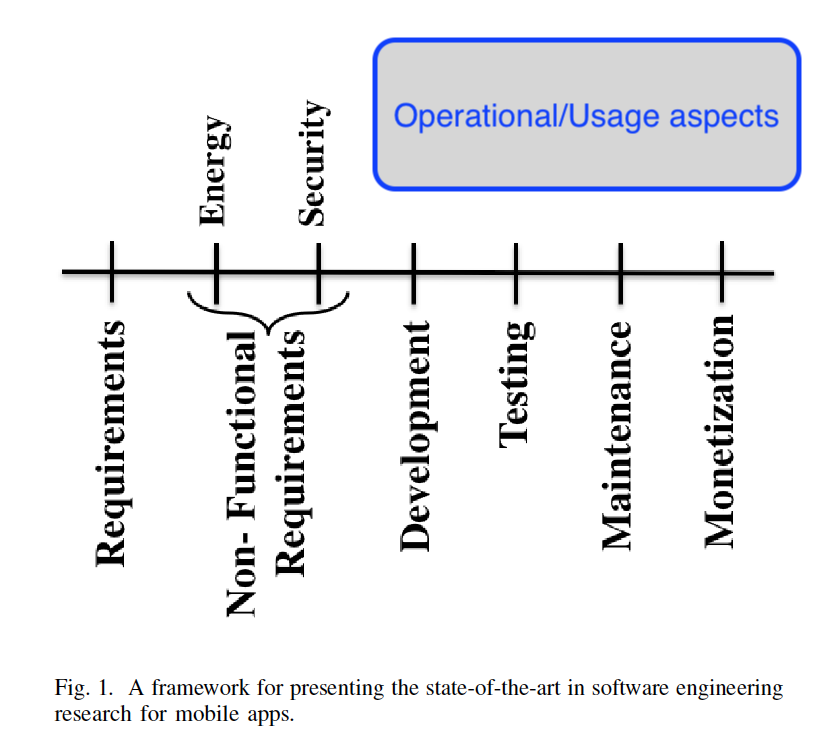
\includegraphics[width=\linewidth]{images/related-work/future-trends-in-sweng-for-mobile-apps-fig-1-annotated.png}
    \captionof{figure}{Annotated version of the framework for presenting the state-of-the-art in software engineering for mobile apps~\cite{nagappan2016_future_trends_in_sw_eng_for_mobile_apps}}
    \label{fig:nagappan2016_future_trends_in_sw_eng_for_mobile_apps_figure_1_annotated}
    } % Thanks to https://tex.stackexchange.com/a/232290/88466

\begin{comment}

\begin{figure}
    \centering
    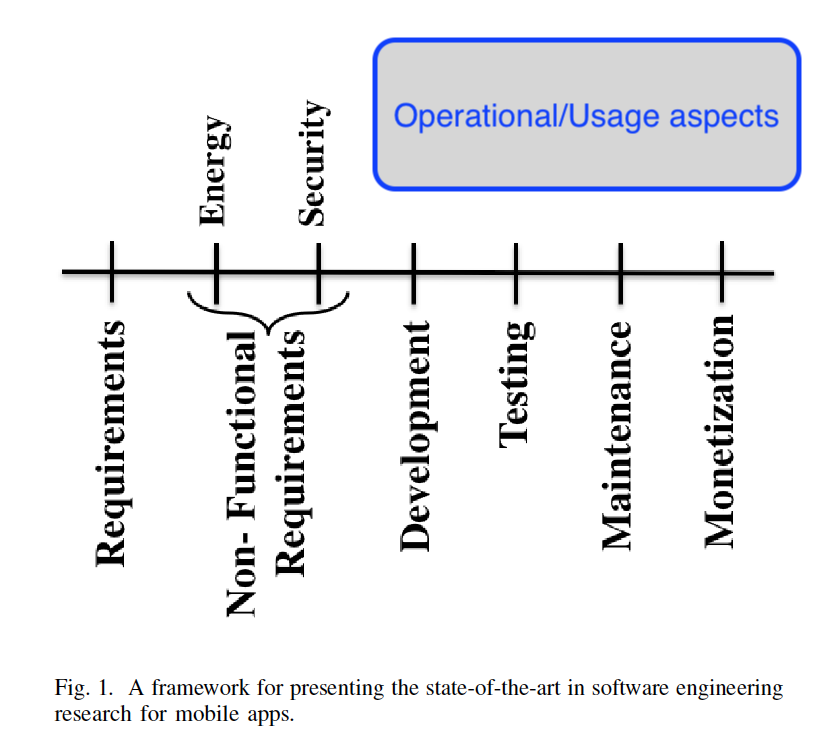
\includegraphics[width=\linewidth]{images/related-work/future-trends-in-sweng-for-mobile-apps-fig-1-annotated.png}
    \caption{Annotated version of the framework for presenting the state-of-the-art in software engineering for mobile apps~\cite{nagappan2016_future_trends_in_sw_eng_for_mobile_apps}}
    \label{fig:nagappan2016_future_trends_in_sw_eng_for_mobile_apps_figure_1_annotated}
\end{figure}
\end{comment}

Mining review data for various forms of data including requests for bug fixes as is using rating as an assessment of goodness. 
Figure~\ref{fig:nagappan2016_future_trends_in_sw_eng_for_mobile_apps_figure_2_annotated} is an annotated version of their Fig. 2 [on p. 23](\textit{ibid}). The annotations include feedback in the forms of ratings and reviews and in the form of mobile analytics. Various sources of information can be used by the development team, of these ratings and reviews are broadly researched, whereas device-level and app-level analytics have not been previously researched.


% Note this could do with expanding while retaining the citation (which leads to Float(s) lost quite often) I'd prefer the proper begin{figure) that's currently commented out.
    {\centering
    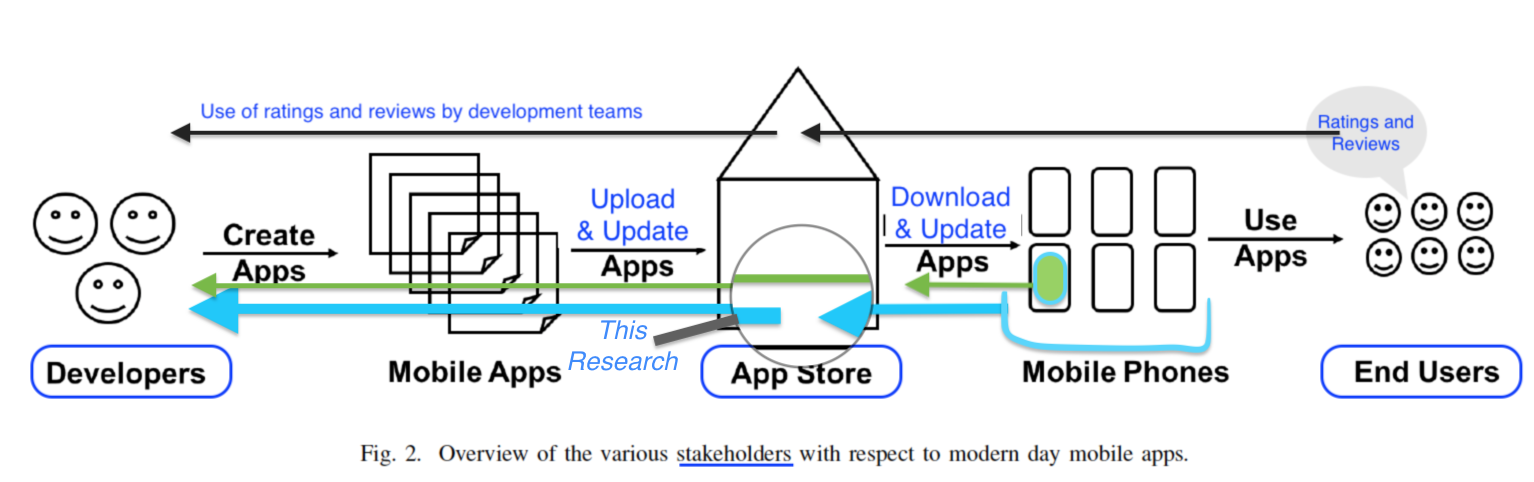
\includegraphics[width=\linewidth]{images/related-work/future-trends-in-sweng-for-mobile-apps-fig-2-annotated-with-highlights.png}
    \captionof{figure}{Annotated version of the various stakeholders in the modern app store ecosystem~\cite{nagappan2016_future_trends_in_sw_eng_for_mobile_apps}}
    \label{fig:nagappan2016_future_trends_in_sw_eng_for_mobile_apps_figure_2_annotated}
    }
  
\begin{comment}
\begin{figure*}
    \centering
    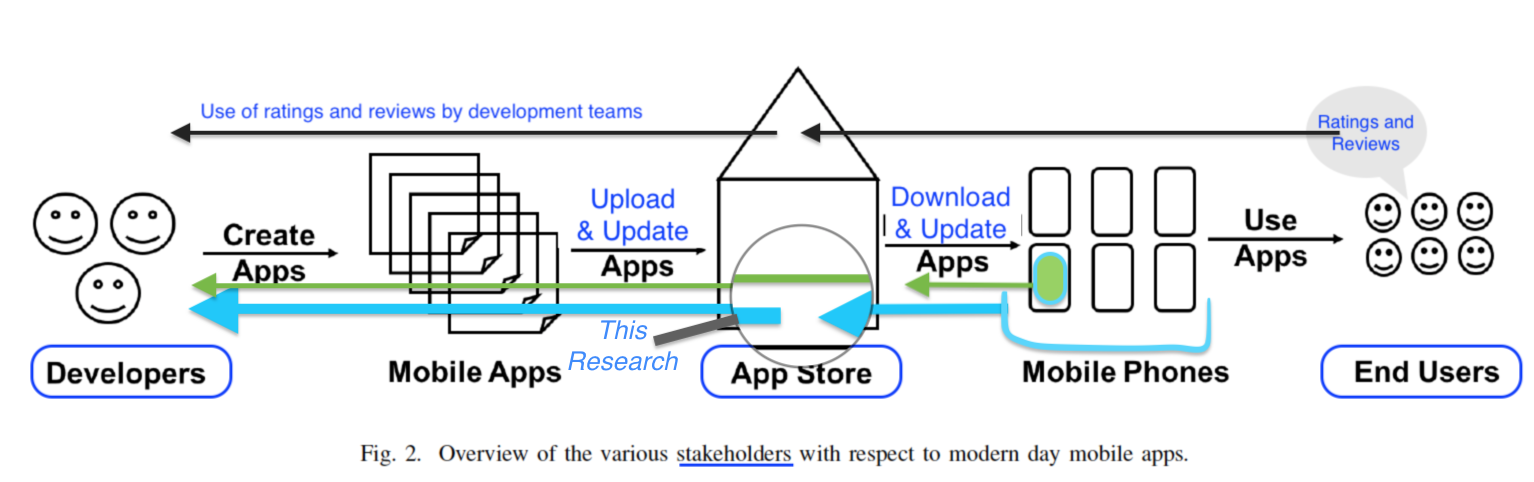
\includegraphics[width=\linewidth]{images/related-work/future-trends-in-sweng-for-mobile-apps-fig-2-annotated-with-highlights.png}
    \caption{Annotated version of the various stakeholders in the modern app store ecosystem~\cite{nagappan2016_future_trends_in_sw_eng_for_mobile_apps}}
    \label{fig:nagappan2016_future_trends_in_sw_eng_for_mobile_apps_figure_2_annotated}
\end{figure*}
\end{comment}  

One of the key challenges identified is restricted access to data held by the app store. The only way they mentioned was to gather historical information by continually mining the app store on a regular basis, [pp 22-23](\textit{ibid}). Perhaps the authors weren't aware that developers of Android apps have access to various historical data about their apps including long term access to all the reviews of their apps. Details of how developers can download these and other reports, including the data structures, are available online~\sidecite{google_play_download_and_export_monthly_reports}.

An area their work did not discuss is whether failure data could, potentially, be a form of requirements? (in a similar fashion to leveraging reviews in the app store to extract `requirements'). And similarly can complaints and failure data be combined to help developers prioritise issues they should consider addressing (the paper restricted the discussion to prioritising issues the developers should be \textit{testing} for).

Finally in terms of this paper, they included two stakeholders, the developers and the end users. The app store (and the people and organisation who provide the app store) are also direct stakeholders in the ecosystem. There are additional indirect stakeholders including advertisers, researchers, and probably many others. 

\subsection{Utility and Service Providers}~\label{rw-utility-and-service-providers-topic}
Developers use software and related services from various providers where the providers are the primary source of any updates. The providers may charge for their offerings and similarly they may mandate various behaviours from developers and their organisations who use the utilities and/or services.

In the context of this research mobile analytics are provided as utilities and/or services by third-parties to app developers therefore it is useful to learn of pertinent research into the use of these utilities and services. Utilities include software tools, libraries, frameworks, and so on; and services may be provided either for some of these utilities or for additional capabilities, support, and so on. Some of the offerings are specific to mobile apps, however many include other platforms such as web sites and/or web apps. Of these examples, an understanding of the use of software libraries helps identify the proclivity of developers to use them and similarly services that apps use are particularly relevant.


\newthought{Libraries: }
Developers can choose to use external libraries to generate revenue (ads)~\sidecite[][p. 407]{li2016_an_investigation_into_the_use_of_common_libraries_in_android_apps}, to \emph{ease the management of HTTP requests}~\sidecite[][p. 73]{belkhir2019_an_observational_study_on_the_state_of_rest_api_uses_in_android_apps} and in their related work they found 98\% of android apps used third-party libraries in their apps~\sidecite[][p. 218]{abdellatif2020_a_multi_dimensional_study_on_the_state_of_practice_of_rest_apis_usage_in_android_app} and on average 41\% of android apps is contributed by common libraries~\sidecite[][p. 409]{li2016_an_investigation_into_the_use_of_common_libraries_in_android_apps}. Using the data in Fig. 5 of this paper (on p. 409) 5\% of the apps included Google Analytics and 2.6\% used Flurry analytics. Note: Industry data indicates mobile analytics are now incorporated in the vast majority of Android apps.  

\newthought{Services: }
Two of the extremely popular categories of third-party libraries are advertising (ads) and mobile analytics.\todo{add examples from research using appbrain examples as a grey data backup/alternative.}
In some ways app developers appear to be similar to their end-users - neither wants to pay up front for what they use.\todo{Add research into the ratio of free to paid apps.} Typically service providers have at least one form of unpaid service offering either time or volume based, many then also have at least one paid-for service offering that do not have the same restrictions of their unpaid offering.

Remote device farms are good examples of services that at least some developers (and/or their organisations) pay for. A relatively dated paper about the then current device farm services provides a useful overview~\sidecite[][]{starov2015_taas_for_mobile_apps_survey} but does not discuss pricing and it predates the now popular service offerings by Google, Amazon, and others. I'm not aware of much research into the use of these device farms apart from some in Brazil IIRC who used an opensource backed test lab service. 

\subsection{Using app store crash analytics to automatically find robustness and reliability failures}~\label{rw-windows-phone-store-crash-analysis-section}
There was a breakthrough stream of work and research that was developed for Microsoft's now defunct mobile app store for Windows Phone devices. That work included mining 25 million crashes~\footnote{Note: The 25 million crashes were a small subset of the total crashes on end-user devices were a subset of the total based on their third footnote ``The developer has no control over the probability.''~\cite[p. 191]{ravindrath2014_automatic_and_scalable_fault_detection_for_mobile_apps}.} that occurred in 2012 on end-user devices when using various apps on their Windows Phones~\cite[p. 190]{ravindrath2014_automatic_and_scalable_fault_detection_for_mobile_apps}. They determined the top 10\% of error buckets covered more than 90\% of crashes~\cite[p. 192]{ravindrath2014_automatic_and_scalable_fault_detection_for_mobile_apps} and discovered a significant proportion of these stemmed from root causes they could generate externally. For example, they could configure a network proxy to return a HTTP 404 response to a network request for network calls made by any of the mobile apps [p. 192].

They built a service called VanarSena to run in the cloud on lots of Windows Phone emulators with the purpose of automatically testing Windows Phone apps. The service automatically instrumented these apps, for instance to add a global Exception handler (the complete set of five injected modules are described in pp. 193..194). The app is exercised using autonomous automated testing tools called~\textit{monkeys} and the service includes a range of fault inducing modules (FIM) [p. 196] that provide inputs and conditions including those that have caused existing apps to crash. 

This paper includes lots of additional practical information that would be pertinent for providers of similar services \emph{e.g.} for other automated testing providers and/or app store providers which we can skip here as they are not closely related to using mobile analytics. Instead, let's concentrate on key characteristics of their work:

\begin{itemize}
    \item Their work built on earlier work of some of the authors where that work was performed at a smaller scale on Android~\cite{ravindrath2012_appinsight_mobile_app_performance_in_the_wild}. They share a common instrumentation framework implemented first for Android then for Windows Phone.
    \item The authors proposed VanarSena could be provided by an app store to help test new releases before they were released in production. The automatic testing helps establish whether the apps handle non-ideal conditions without crashing.
    They describe crash buckets and a) identified commonalities in those crash buckets, b) found a significant subset could be triggered through manipulating inputs, conditions, and responses to the app.
    \item The results of their research included finding 1108/3000 production Windows Phone apps had failures that were detected by VanarSena. They uncovered 2969 distinct bugs in these apps including 1227 that were not previously reported~\cite[p. 202]{ravindrath2014_automatic_and_scalable_fault_detection_for_mobile_apps}. Some of the failing apps had been developed by professionals others by amateurs - this indicates developers often write code that does not cope adequately with non-ideal circumstances.  
\end{itemize}

Several of the authors of the previous paper collaborated with other colleagues at Microsoft Research to extend the work. In ~\textcite{chandra2015_how_to_smash_the_next_billion_mobile_app_bugs} they describe various improvements to their Caiipa service that delivered eleven-fold more crashes and eight-fold more performance problems~\cite[pp. 37-38]{chandra2015_how_to_smash_the_next_billion_mobile_app_bugs}. The core of their paper presents their plans for a sophisticated automated testing system for testing Windows Phone apps together with their goals and challenges. The most pertinent goal in terms of this research would be actionable reports~\cite[p. 36]{chandra2015_how_to_smash_the_next_billion_mobile_app_bugs} together with their use of context data and historical data. 

Given the nature of Microsoft's objectives they did not consider Mobile Analytics or crash reporting SDKs (which include breadcrumbs and the ability to report caught errors, \emph{etc.}). Nor do their papers mention how the app developer's perceived their various tools and services. It's unclear whether they actually involved app developers in their work. Also, given the demise of the Windows Phone platform and app store it appears much of this work has disappeared without a trace.


\subsection{Power dynamics}~\label{rw-power-dynamics-topic}
Grey literature is the main source of the imbalance in power between app developers and the app store, at least in terms of Google Play and Android apps in that store. I have selected four illustrative articles, by four different developers, of the 20+ related articles published on \href{https://medium.com/}{Medium} % More material is available on corporations on mining data from the public  from and via https://jilliancyork.com/
about how they lost access to their apps and in some cases their account. 

In \textcite{martinez2019_google_just_terminated_our_startup_google_play_publisher_account_on_xmas_day} the termination of a personal Google Play account for an indirectly associated developer, via one of the employees of the small company, was attributed to the termination of that company's Google Play account. This story has ongoing updates that lists various developers who have had similar experiences. A similar experience was reported by \textcite{dodson2019_google_completely_terminated_our_new_business_etc} where apparently someone's associated account was the cause of Dodson's account being terminated. As Méa dry noted \emph{``google@play-store: sudo rm -rf org.mtransit.android*''} which happened abruptly within a few hours of sending an email notification to the developer. The reason given in the automated emails was the app was in violation of the ``Deceptive Behavior policy''~\sidecite{mea2019_google_just_deleted_my_nearly_10_year_old_app_etc}. 

In these three instances the developer accounts were reinstated. In \textcite{marcher2021_how_google_terminated-a-developer} the account was not reinstanted and two of his clients also had their accounts terminated. As Marcher notes \emph{``I develop software not just for fun but also primarily for a living. This action not only deprives me of a substantial part of income, but it also forbids me for life to continue my work which is also my passion''}. % See also https://medium.com/@appsrentables1/google-cancels-our-google-play-publisher-account-and-ends-my-familys-source-of-income-97d4e85cd046 and various others (20+ stories)

\subsection{Developers and their app counts}
Before we leave the topic of App Store ecosystems and in particular a developer focused perspective on the ecosystem, the work of \textcite{wang2017_exploratory_study_of_the_mobile_app_ecosystem} looks potentially interesting as it states it looked at the Google Play store from a developer's perspective; the title appears misleading as they actually researched mappings between developers and the number of apps they had in Google Play Store. In other words, the paper concentrates on the characteristics of developers who have many apps in the app store rather than on the software development/engineering aspects.

They estimated there were 320,000 developers, over half of the developers only released a single app. The paper main focus though is on the \emph{``the group of aggressive developers who have released more than 50 apps, trying to understand how and why they create so many apps''}. In terms of this research this paper provides some context on who writes the mobile apps in Google Play, provides an estimate of the population of developers (in 2017).


\section{Developing Mobile Apps}~\label{rw-developing-mobile-apps-section}
Research into the development practices and mechanisms for mobile apps establishes various norms, characteristics, and habits, of app developers. Their work, collectively, is used by billions of people throughout the world. In terms of this research, understanding the development practices and mechanisms is vital. Developers also have a voice and hundreds have been interviewed to learn what's important to them, for example in \sidecite{joorabchi2013_real_challenges_in_mobile_app_development}. They also communicate through various artefacts they create and maintain, again these artefacts have been studied to learn about their work, for example in \sidecite{pascarella2018_self_reported_activities_of_android_developers}.

% Some of the effects of their work in terms of software quality will be covered later in this chapter in \secref{rw-mobile-app-crashes-topic}.

Mobile apps need to be made and developers make them. There are various working practices, apps are made by visionaries, employees, amateurs, and communities. There are various activities involved including development, testing, release, and deployment. % Figure~\ref{fig:my_mobile-app-makers} highlights these activities as part of the overall ecosystem.

% Many mobile app development teams would describe their development practices as Agile or based on along the principles of Agile development. % Solo app developers are less likely to use these practices, nonetheless there has been various research into adaptions of Agile and Scrum in attempts to suit them. Various examples are in the excluded-bibliography.
% Many of these people claim to be ``Agile" in their working practices.

5,000 commit messages (of over 1.8 million identified) were studied that were selected from 8,280 active opensource Android apps where the source code repositories were on github.com. The top three activities were 1) app enhancement, followed by 2) bug fixes, and then 3) project management~\sidecite[][p. 144]{pascarella2018_self_reported_activities_of_android_developers}. 35 of the commit messages were attributed to addressing crashes in the app [Figure 3, on p. 151]. They did not investigate how developers had discovered issues nor whether mobile analytics were affected in the commits, leaving these aspects unknown and unreported.

Relatively early research, published in 2013, identified several key topics of concern for app developers including: a strong need for monitoring and analysis support, for instance to monitor the health of an app. Similarly a major problem was crashes \emph{``which are often intermittent, non-deterministic, and irrecoverable.''}~\sidecite[][p. 21]{joorabchi2013_real_challenges_in_mobile_app_development}. Interestingly, one of the discussion topics was to research testing \acrshort{api}s from App Stores[pp. 22-23] which predates Google Play's Pre-launch reports covered in \secref{tata-pre-launch-reports-topic}.


As mentioned previously, in \secref{rw-utility-and-service-providers-topic}, Android apps incorporate software libraries extensively~\sidecite{li2016_an_investigation_into_the_use_of_common_libraries_in_android_apps}. The extensive use of software libraries, generally provided by third-parties, indicate the developers place significant trust with these third-party developers. Also, their apps contain large volumes of code that is \emph{unlikely} to have been tested by the app developers apart from some sanity and/or smoke testing. Flaws and instabilities in these libraries may be latent until the app is being used at scale by end users. How will the developers learn about the effects of emergent flaws and instabilities?

Note: in terms of trying to understand real-world practices please avoid \textcite{santos2016_investigating_the_adoption_of_agile_practices_by_20_undergrad_students_in_mobile_app_devt} which sounds relevant but only surveyed 20 undergraduate students who took an iOS development course. 

\subsection{Testing Mobile Apps}~\label{rw-testing-mobile-apps-topic}

There has been a tremendous amount of research into practices and tools that might perform better than the mainstream test automation tools available to app developers.

A useful categorisation of testing for mobile apps may be: 
explicitly designed scripted tests, 
automatic robots that navigate and sometimes interrogate target apps, and 
hands-on testing which often vary depending on who performs them and each instance of the testing. 
Where the testing may be performed:
on local physical devices,
on remote physical devices in the `cloud'
on local emulators and/or local simulators, and
on remote emulators and/or simulators.


There has been a lot of research into various artefacts pertaining to mobile apps. Some of the artefacts are mainly generated by end users, for instance ratings and reviews, and others are mainly generated by software developers such as source code. A hybrid artefact are bug reports. These also known as issues particularly for projects based on github.com as it uses that term and developers create bug reports as issues on github.com. Bug reports are a hybrid artefact as potentially anyone can create them including users of the code and the development team. 

That said, for the projects studied in this research they mainly used `issues' and these were mainly created by the project's extended development team (an extended development team may include people involved in project management and/or testing).

\subsubsection{Papers to consider}
\begin{itemize}
    \item Discuss the TestDroid paper! it describes testing that was actually done by developers!~\cite{kaasila2012_testdroid_etc}.
    
    \item \emph{``Is Mutation Analysis Effective at Testing Android Apps?"}~\cite{deng2017_is_mutation_analysis_effective_at_testing_android_apps}.
    
    \item \emph{``Mining Android Crash Fixes in the Absence of Issue- and Change-Tracking Systems"}~\cite{kong2019_mining_android_crash_fixes}.
    
    \item \emph{``How do Developers Test Android Applications?"}~\cite{linares2017_how_do_developers_test_android_apps}. Quote:~\emph{``“I mostly do manual testing due to the limited size of my apps. I sometimes use a custom replay system (built into the app) to duplicate bugs after I come across them. This method is usually combined with manual testing (printing debug information to the log) to pinpoint the cause”."}
    
    \item \emph{``First Steps in Retrofitting a Versatile Software Testing Infrastructure to Android"}~\cite{oliver2018_first_steps_in_retrofitting_a_versatile_sw_testing_architecture}.
    
    \item \emph{``A Large-Scale Study of Application Incompatibilities in Android"}~\cite{cai2019_large_scale_study_of_android_incompatibilities} An oddly insipid paper which promised some interesting run-time issues discovered in their research where the Android version would be a likely cause. However the reproduction package lacked the test scripts or means to reproduce their testing or bug detection. Also, their research now seems to be less relevant in 2020 as Android apparently improved the backwards compatibility \emph{``Yet newer versions (since API 24) had no run-time compatibility issues with apps created in the studied span."}. Their work may well have merit for the research community, It does not appear to have much relevance to developers of real-world Android apps today.
    

    \item \emph{``Intent Fuzzer: Crafting Intents of Death"}~\cite{10.1145/2632168.2632169} TODO Link this to the industrial case study and the Kotlin NPE crash.
    
    \item \emph{``Linares-Vasquez et al. [56] propose MonkeyLab, which mines recorded executions to guide the testing of Android mobile apps."} Their approach records GUI events (click events). Members of the project team (developers, testers, etc.) perform the actions, the authors claim their log collection process could scale to collecting logs from ordinary users. Key limitations include events that aren't purely dependent on the user's GUI inputs, there would also be challenges getting users to accept such an approach where the app records every input they made. Also, they generate GUI events that have x,y coordinates - absolute positioning that may have limited portability to other devices, screen rotations, and so on. Their playback also appears to require rooted devices. There are numerous other limitations described in their paper, nonetheless their work shows promise in terms of detecting and generating patterns the students did not find. It would be interesting to compare the results using accomplished software testers with experience and expertise testing similar Android apps.
    
    \item \emph{``An Empirical Study of Android Test Generation Tools in Industrial Cases''}~\cite{wang2018_an_empirical_study_of_android_test_generation_tools_in_industrial_cases} 
\end{itemize}

There has been a tremendous and sustained research interest in software testing, for instance testing is one of the most popular topics at the ICSE series of conferences~\footnote{\url{https://dl.acm.org/conference/icse}} and the focus of entire conferences including AST~\footnote{\url{https://conf.researchr.org/home/icse-2020/ast-2020}}, ICST~\footnote{\url{https://conf.researchr.org/series/icst}}, and so on. Similarly the application of software testing to mobile apps is a rich topic with sustained interest in the challenges and facets of testing mobile apps.

The facets include automated testing and automated bug reproduction, maximising the `bang for the buck' for instance in selecting which device models would be most valuable to use with finite testing. Understandably given the field where many of the authors work - in research - the vast majority of the research is on software apps they have access to, software their can obtain the source code for (particularly opensource), software they can write, and the people they have available to them (other researchers, students, voluntary participants, and people paid to paid to perform specific tasks). Minute amounts of the work is based on mature, popular software with semi- or fully- professional developers and development teams. Some research projects, particularly CRASHSCOPE~\cite{moran2016_automatically_drr_android_app_crashes}, offer the potential to reproduce some of the crashes reported by Mobile Analytics if the tools are sufficiently available and current to actually use.




\subsubsection{Prioritising devices to test on}

Selection criteria include:
\begin{itemize}
    \item the relative popularity of a single app across the user base for the app, provided by OpenSignal, and reported over a three year period,
    \item the usage of similar, popular, Android apps for two app categories: grouped by device model as measured by a very popular app management app in China,
    \item the devices used most frequently by users who write reviews for the same Android app,
\end{itemize}

One of the research papers close to the area of my research uses usage data for two popular app categories (games and media) gathered through a popular Android management app in China~\cite{lu2016_PRADA}. Their work uses an operational profile to prioritise the device models to select to test both new or existing apps. The management app, called Wandoujia~\footnote{\url{https://www.wandoujia.com/}}, is used by \emph{`500 million people to find apps they want`}~\footnote{According to Chrome Browser's automatic translation from Chinese.}. Daily usage of the top 100 apps in the two app categories was collected for various device models. In various ways the Wandoujia app management app provides similar capabilities to Google Play, including tracking when apps are installed, and in use. The recommendations are coarse-grained. The research measured the accuracy of their predictions for recommended devices with the actual devices that the app ended up being used on once the app had been launched. 

Their work demonstrates that usage data for several app categories was useful to guide developers on the most popular actual device models for their app. They acknowledge several limitations in their work, including their use of incomplete measures such as foreground network activity for usage which don't suit apps that either perform network processing in the background or don't use the network. Other app management services, particularly Google Play, could provide similar guidance to app developers. And indeed as Google Play collects additional data for the entire apps store it could cover some of the gaps and limitations identified in this research.


\subsubsection{Device Testing Services}
Test Farms have been available commercially since around 2008~\footnote{Based on the author's professional experience.}. Over the years different offerings have peaked and then either been acquired, retired, or disappeared. Google, Amazon and Microsoft offer paid-for device farms as do various specialist businesses. There have been a couple of public-good initiatives including Open Device Labs~\footnote{For example~\url{https://opendevicelab.com/},~\url{https://www.devicelab.org/}}; and Open STF~\sidecite{openstf_website} which is based on a set of opensource projects~\url{https://github.com/openstf/} and enables teams and organisations to build their own device farms or use commercial offerings based on these projects~\footnote{For example~\url{https://www.headspin.io/}.}.
% https://loadfocus.com/blog/tech/2018/04/building-your-in-house-device-farm-on-mac-os-using-openstf-for-android-testing/ 
% https://tech.mercari.com/entry/2019/02/18/173236 (on using HeadSpin and NimbleDroid).



\subsection{Maintenance of mobile apps}

\emph{``The area of software maintenance is one of the most researched areas in Software Engineering. However, due to the fact that mobile apps is a young subarea within SE, the maintenance of mobile applications remains to be largely undiscovered."}~\cite[p. 27]{nagappan2016_future_trends_in_sw_eng_for_mobile_apps} - My work does investigate aspects of maintenance. 

\emph{``Syer et al. [93] compares mobile apps to larger “traditional” software systems in terms of size and time to fix defects. They find that mobile apps resemble Unix utilities, i.e., they tend to be small and developed by small groups. They also find that mobile apps tend to respond to reported defects quickly."}~\cite[p. 27]{nagappan2016_future_trends_in_sw_eng_for_mobile_apps} - Check the details of what quickly means and how the teams discovered the defects.

\emph{``Bavota et al. [16], show that the quality (in terms of change and fault-proneness) of the APIs used by Android apps negatively impacts their success, in terms of user ratings. Similarly, McDonnell et al. [65], study the stability and adoption rates for the APIs in the Android ecosystem."}~\cite[p. 27]{nagappan2016_future_trends_in_sw_eng_for_mobile_apps} - Skim read both these papers to determine their relevance.

\emph{``Another line of work examined Android-related bug reports. Bhattacharya et al. [18] study 24 mobile Android apps in order to understand the bug-fixing process. They find that mobile bug reports are of high quality, especially for security related bugs. Martie et al. [63] analyzed topics in the Android platform bugs in order to uncover the most debated topics over time. Similarly, Liu et al. [58] detected and characterized performance bugs among Android apps."}~\cite[p. 27]{nagappan2016_future_trends_in_sw_eng_for_mobile_apps} - Looks at how the bugs were fixed and compare the practices they detected with those I'm aware of. Are platform bugs that relevant? They look at performance bugs (Android Vitals also reports performance issues, Firebase Analytics has tools for performance tracking), I'm looking mainly into reliability measurements and issues.

Following on from the challenges and future directions section on maintenance research for mobile apps: do researchers focus in areas where the streetlights are rather than where the problems are? \emph{i.e.} on where they can find material to study rather than on issues that practically affect the majority of developers of apps?

\emph{``Charting the API minefield using software telemetry data"}~\cite{Kechagia2015_charting_API_minefield_using_telemetry_data}. The stability of Android apps has been measured using telemetry data collected by a centralised crash report management service. Roughly one million stack traces were analysed from thousands of Android applications. A subset (over 500,000) of these stack traces were associated with risky API calls and these were analysed to identify the most common failure reasons. The top five reasons were attributed to:
    \begin{itemize}
        \item memory exhaustion,
        \item race conditions,
        \item deadlocks,
        \item missing resources, and
        \item corrupt resources.
    \end{itemize}
    
    The authors provide a set of recommendations they claim \emph{may} help address various classes of the crash failures. However these recommendations do not appear to have been tested for their efficacy. Their recommendations are theoretical rather than practical. There's an odd claim in the paper in page 1818, \emph{``In addition, the platform of Chen et al. (2011), which is based on remote resource management, can make applications require less memory and resources. Hence, it can eliminate the well-known “non-responsive” exceptions in Android."}. For this claim to hold true \textbf{all} the causes of non-responsive exceptions (or did the authors mean ANRs? they don't define this term or use it elsewhere in the paper) would need to be a) related to remote resources, and b) the difference would need to be directly related to the amount of memory and resources. Google provides five common patterns for diagnosing ANRs~\footnote{\url{https://developer.android.com/topic/performance/vitals/anr\#diagnosing_anrs}} none of these mention remote resource management (even if they may contribute to ANRs). The authors say in the introduction to section 5.1~\emph{`API Recommendations'}, on page 1813,~\emph{``Finally, we provide the frequencies of the representative signatures to show how many crashes could be avoided based on the following solutions."}, however they did not appear to provide this unless they are the charts in  Appendix 1 \textbf{\textit{and}} if their proposals solve \textit{all} the causes of the crashes in each category. This was promising, thought-provoking, and interesting work which sadly lacked evidence their proposed recommendations actually work in practice for any of the apps that provided the crash data or for other Android apps (if their work is generalisable).


\subsection{Managing Releases in App Stores}
% Julian continue here...

\emph{``Release Practices for Mobile Apps--What do Users and Developers Think?"}~\sidecite{nayebi2016release}.
    
\emph{``Towards Release Strategy Optimization for Apps in Google Play"}~\cite{shen2017_towards_release_strategy_optimization_for_apps_in_google_play}. ``empirical study to help developers decide the release opportunity to maximize positive feedback from users at scale.". They identify three patterns of update intervals: successive, normal, sparse. Their work does not use signals such as the stability of the app. They also claim ``Additionally, app quality can be unstable with fast [release] iteration[s]."

    
The \emph{``Data analytics for decision support in software release management"}~\cite{didar2018data_analytics_phd_thesis}, a PhD thesis, introduces a proposed Plan-Monitor-Improve Framework for release management.

\emph{``Revisiting Prior Empirical Findings For Mobile Apps: An Empirical Case Study on the 15 Most Popular Open-Source Android Apps"}~\cite{syer2013_empirical_findings_for_mobile_apps} is work from 2013 (when Google Code was still a major active public source code repository) that compares the codebases of 15 opensource mobile apps with 5 other opensource desktop/server projects. A key finding in their research includes the development process - where there are frequent releases yet the development and release processes are immature. albeit based on codebases from 2011 so a decade ago is still relevant. They ask various open-ended questions:
    \begin{itemize}
        \item Does such a high frequency of releases mitigate the lack of testing? 
        \item If there are frequent releases for the mobile app, then does quality matter as much?
        \item Is the project in a constant beta testing state? 
        \item Does the platform provide sufficient support for building high quality apps quickly? 
        \item Is the frequent release only influenced by the demand factor in the app store? 
        \item Are the developers of mobile apps more skilled or do they have more resources at hand? 
        \item Or, are mobile apps themselves less complex to develop?
    \end{itemize}
    
Perhaps the cost of failures in the app store was/is perceived to be low in the Google Play app store, at least for these 15 opensource apps? Later work investigated aspects such as the release frequency~\sidecite{nayebi2016release}

    
\emph{``Are apps ready for new Android releases?"}~\textcite{guilardi_are_apps_ready_for_new_android_releases} flips the perspective from when developers should release their apps to asking how well developers keep up with new releases of Android. This is a relatively recent paper where the researchers discovered that developers are slow to revise and update their Android apps for new releases of the operating system. Some of the apps have flaws exposed when running on new versions of the operating system. For apps to retain their quality they need to be updated, new releases of the operating system are one such reason. (Releases of libraries another, new contexts of use, etc. another...).


As we will discover later in this thesis Google Play Console includes a set of live release management reports aimed at helping app developers observe the effects of a new release as it's rolled out to the userbase. They also use popularity of the app in various regions to control automated pre-release testing of new releases of an app.\todo{Add forward links to these two topics in those chapters.}


\section{Sources of information on software quality for developers of mobile apps}~\label{rw-sources-of-info-on-software-quality-for-devs-of-mobile-apps}
Feedback comes in various forms in an app-store ecosystem, ratings and reviews are two of them and possibly the best known ones because they are public and highly visible to end users and anyone else who wishes to see them. As part of scoping this research at least fourteen distinct forms of feedback have been identified~\footnote{As discussed in the previous section, it's not clear whether the test results of Microsoft's work on Caiipa, VanarSena, and SMASH was ever presented to the developers of the Windows Phone apps Microsoft tested. Nonetheless it could be incorporated into this work as and when it is presented, it appears similar to pre-launch reports in Google Play yet significantly more capable.}, these are presented in Table~\ref{tab:feedback-sources-about-their-app-for-devs}.

The feedback source is mainly from humans for: ratings, reviews, social media, email to the dev team, manual testing, and code reviews. The feedback sources for the other sources are mainly automated. Developers need to be involved in setting up many of the feedback sources and they choose which ones to act on.

Note: the following sources of feedback are not limited to mobile apps within an app store they can be used for other software, however these are outside the scope of this research.

End users can provide feedback through other public channels such as social media (Twitter and Facebook being the largest and best known), or through a variety of private channels ranging from email (Google Play displays the contact email address for each app developer in the Google Play Store) to in-app feedback. Several of these will be mentioned as examples otherwise they're also beyond the scope of this research for various reasons. 

Feedback can also be generated by software at run time. These include GUI-oriented utilities such as heatmapping tools (covered in \secref{section-heatmapping}, application-oriented utilities including logging and mobile analytics, and platform-oriented tools.

%Feedback can also be obtained at a per-project level

\pagelayout{wide} %  % Restore full width, from https://tex.stackexchange.com/a/606261/88466

\begin{table}[H]
	\setlength\tabcolsep{0.4em} % Horizontal whitespace between columns
	\def\arraystretch{1}% Override the default row height set in latex-configuration.tex
	\scriptsize % Reduce font size
	\begin{tabular}{L{2cm} L{2.4cm} L{3.5cm} L{2.4cm} L{3.5cm}} % Column alignment and width specification
		\toprule
		\textbf{Source} & \textbf{App-store ecosystem} & \textbf{User-base scale} & \textbf{Individual-project} & \textbf{Remarks} \\ \midrule
		Ratings & Yes & Yes & No & Ratings can be provided without a review. \\ \midrule
		Reviews & Yes & Yes & Not really & Extensively researched \\ \midrule
		Social Media & No & Yes & Unlikely & N/A for many apps. \\ \midrule
		In-app feedback & No & On a per-app basis & Yes & N/A for many apps. \\ \midrule
		Email to dev team & Not really & On a per-app basis & Yes & Oft-ignored? \\ \midrule
		In-app Mobile Analytics & Varies~\footnote{Firebase - somewhat, otherwise less so. Mainly compatible (except F-Droid).} & Yes & Yes & Very popular, distinct from the app store, yet close cousins. \\ \midrule
		Platform Analytics & Yes & Yes & Yes, for high-volume released apps. & Reports are not available for low volume apps and those with few detected failures.  \\ \midrule
		Automated unscripted Testing & Only as part of the pre-launch reports & N/A & Yes, generally available free-of-charge & Works at a platform level, e.g. for many apps on that platform without needing in-depth custom scripts\footnote{ Some apps, and therefore some tools support scripts for login to an app, and/or scripts that bootstrap testing to start at the right place in an app. Robo is a good example of this sort of tool. The tools then explore an app using their own internal algorithms.}. \\ \midrule
		Manual Testing & Only when using test tracks to release the software to the manual testers & Not generally~\footnote{Crowd-based testing is covered in various research; AFAIK the largest scale is Huawei testing a fix for ANRs (re: sd-card writes).} & Yes, often used to some extent. & Used piecemeal by the majority of devs. Not necessarily done well. Not necessarily done by ‘testers’ or ‘users’ i.e. non devs. \\ \midrule
		Automated scripted tests  & No~\footnote{however several connected services offer remote device test labs which can be used for testing new releases.} & No & Yes if devs have created them. & If the development team has created them then they probably also run them as part of the CI/CB mechanisms. \\ \midrule
		Heatmaps (Visual Analytics Replay) & No & No (unlikely to pass privacy legislation/constraints) & Yes, requires the developers to integrate an SDK and use a service. & My impression is they’re used by exception only these days. \\ \midrule
		Pre-launch reports & Yes & N/A & Yes, provided the team chooses to create test releases in Google Play. & These include static analysis and automated unscripted testing. They also combine platform analytics. \\ \midrule
		Static Analysis Code Quality tools & Only as part of the pre-launch reports & N/A & Yes & Freely available, perceived as noisy. \\ \midrule
		Code Reviews & No & No & Yes & Oft practiced by teams \\
		\bottomrule
	\end{tabular}
	\caption{Feedback sources about their app for developers}
	\label{tab:feedback-sources-about-their-app-for-devs}
\end{table}


\vspace{2\baselineskip}
\pagelayout{margin} % use large margins

\subsection{Ratings in app stores}

%\subsection{Venn Diagram of feedback sources for developers}
% I've sketched out a Venn diagram that led to the development of Table \ref{tab:feedback-sources-about-their-app-for-devs} however Marian warned me not to get myself into a rabbit hole trying to write up these forms of feedback. The Venn diagram would be part of that writing up so for now I'm hiding it from the generated doc.

\begin{figure}
\RawFloats
\centering
\begin{minipage}{.4\textwidth}
  \centering
  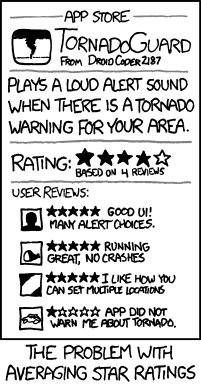
\includegraphics[width=\textwidth]{images/xkcd/tornadoguard.png}
  \captionof*{figure}{TornadoGuard \url{https://xkcd.com/937}}
  \label{fig:xkcd-tornadoguard}
\end{minipage}\hfill%
\begin{minipage}{.5\textwidth}
  \centering
  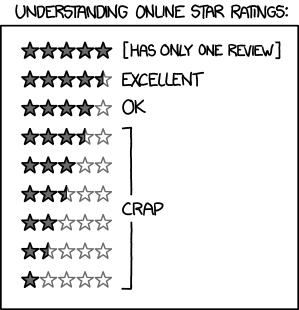
\includegraphics[width=\textwidth]{images/xkcd/star_ratings.png}
  \captionof*{figure}{Understanding online star ratings \url{https://xkcd.com/1098}}
  \label{fig:xkcd-star-ratings}
\end{minipage}
    \caption{XKCD's views on App Store Ratings and Reviews}
    \label{fig:xkcd-app-store-ratings}
\end{figure}
% https://www.explainxkcd.com/wiki/index.php/937:_TornadoGuard
% https://www.explainxkcd.com/wiki/index.php/1098:_Star_Ratings


Apps with poor ratings are less likely to be downloaded by new users~\sidecite{dimensionalresearch2015_mobile_app_use_and_abandonment}. Ratings also affect where an app appears in search results and whether an app store will choose to promote that app, or another. In the author's experience when one team's Android app's overall rating dropped from 4.4 to 4.3 stars the business noticed an almost immediate reduction in revenues from the app in addition to discovering that app was ranked lower in the search results. Therefore ratings are an important measure for app developers, and one they may choose to influence positively. 

Gaming ratings includes activities such as an app first asking if a user is happy with the app, and if they say yes then providing a link to encourage the user to rate the app positively in the app store. \textcite{novoda_akan2016_asking_for_app_feedback_the_effective_way} provides an illustrative industry case study of how Novoda improved the rating of a major newspaper's app. And in terms of the SDKs developers can use for in-app feedback, Apptentive is one of several companies that provides SDKs to help developers optimise their ratings and reviews and guides on how to do so within a mobile app~\sidecite{walz2015_apptentive_the_mobile_marketers_guide_to_app_store_ratings_and_reviews}. Unsurprisingly, ratings are also a subject of research interest.

Here are several representative papers that focus on engineering aspects of ratings and reviews.  \textcite{alsubaihin2019app_store_effects_on_software_engineering} discusses the symbiotic relationship between releases and the ratings and reviews that app received [p. 14]. Some developers time their releases based on the feedback they've received and monitor ratings and reviews for their latest release to influence the rollout of the new release. There have been innovative ideas on using ratings to prioritise software engineering activities including software testing of Android games apps~\sidecite{khalid2014_prioritizing_the_devices_to_test_your_app_on_casestudy_android_games}. And in \textcite{greenheld2018_automating_developers_responses_to_app_reviews} the value of developers responding to reviews was highlighted. 
In a population of 10,000 Android apps extracted from Google Play, correlations was identified between the density of warnings reported by FindBugs, a static analysis tool, and app store reviews and ratings for these apps~\sidecite{khalid2016_examining_the_relationship_between_findbugs_warnings_and_app_ratings}. They considered three warning categories: bad practices (which include reports of crashes in the reviews), internationalisation, and performance (which might relate to ANRs, however they didn't investigate this aspect). They did not investigate whether addressing warnings from FindBugs improved the ratings or reviews for those apps, and mobile analytics was not mentioned in their work - unsurprising as they took a black box approach using decompiled Android app binaries.

Via Figure \ref{fig:xkcd-app-store-ratings} XKCD aptly sums up two facets of flaws in app store ratings and reviews, averaging reviews may not be a good measure~\sidecite{explainxkcd_937_tornadoguard}, and the star ratings are not treated as a linear scale in practice~\sidecite{explainxkcd_1098_star_ratings}. In summary, app Store ratings therefore may not be an ideal measure of the quality of an app from a software engineering perspective! 
% See also stanik2020_requirements_intelligence_on_the_analysis_of_user_feedback
% shen2017_towards_release_strategy_optimization_for_apps_in_google_play 

\subsection{Reviews in app stores}
Similarly reviews in app stores have been analysed for various purposes including for complaints and bug reports. Of the many and various research on reviews of mobile apps in app stores. 
Two early papers, the first focusing on Android apps in Google Play~\textcite{fu2013_why_people_hate_your_app_making_sense_of_user_feedback_in_a_mobile_app_store} and the second for iOS apps in Apple's App Store~\textcite{khalid2015_what_do_mobile_app_users_complain_about}.

In \textcite[p. 5][]{fu2013_why_people_hate_your_app_making_sense_of_user_feedback_in_a_mobile_app_store} the top three most common indicators of problems in the apps were: slow 9,939, crashes 9,081, and freezes 3,960. Stability was a common theme of complaints about both free and paid apps [pp. 7-9]. 

In \textcite{khalid2015_what_do_mobile_app_users_complain_about} clearly establishes connections between what users of iOS apps complain about and the effects of these complaints on ratings of those apps; and \textcite{panichella2015_how_can_i_improve_my_app_classifying_user_reviews_for_sw_maintenance_and_evolution} extends that work to consider the relevance of various review-topics to developers. Panichella \emph{et al} also extend the work to include Android apps in the Google Play Store. \textcite{mcilroy2016_analyzing_and_automatically_labelling_the_types_of_user_issues_raised_in_mobile_app_reviews} - labels the content of reviews extracted from Google Play and found crashes and crashing were one of the topics that was a) relatively easy to categorise, and b) occurred frequently. This paper seemed to conflate in-app analytics tools (Flurry) with analytics of reviews (e.g. AppAnnie). As an observation, since this paper was published Google Play now provides automated labeling and analysis of reviews.

Feedback comes in various forms, ratings and reviews are only two of them.  One that's seldom used in industry and seldom researched is implicit feedback recorded through user-interactions with the GUI of the mobile app. Common terms for this mechanism include `heatmaps' and `heatmapping' and there are commercial SDKs and opensource projects available that perform the recording within an app at runtime. The elixir of automating `record and playback' test automation sometimes uses similar methods to record the interactions with a mobile app. 

\subsection{Testing}
\emph{``How do Developers Test Android Applications?"}~\sidecite{linares2017_how_do_developers_test_android_apps}. Quote:~\emph{``“I mostly do manual testing due to the limited size of my apps. I sometimes use a custom replay system (built into the app) to duplicate bugs after I come across them. This method is usually combined with manual testing (printing debug information to the log) to pinpoint the cause”."}

The absence of automated tests does not prove developers do not test their Android apps, rather it indicates their projects are unlikely to have any automated tests and similarly that the project is unlikely to run any automated scripted tests as part of a continuous build. (In honour of Dijkstra's observation that ``Testing shows the presence, not the absence of bugs'', Edsger W. Dijkstra in ~\textcite[p. 16][]{randell1970_software_engineering_techniques_nato_dijkstra}.) % Found via https://en.wikiquote.org/wiki/Edsger_W._Dijkstra
% See also: https://www.techwell.com/techwell-insights/2018/12/can-we-ever-find-all-bugs 
% https://wiki.c2.com/?TestsCantProveTheAbsenceOfBugs

An incredible amount of research energy has gone into trying to find better ways to test mobile apps, ranging from autonomous tools that where the researchers endeavour to deliver better coverage than a small free utility called \texttt{monkey} (and sometimes manage to do so), through to ways to generate automated tests from the text of reviews. Virtually none of these endeavours seem to make any difference to the testing developers do, they don't use the tools developed from these research efforts. 

\emph{``Thus even if the app is tested on one device, there is no guarantee that it may work on another device."}~\cite[p. 27]{nagappan2016_future_trends_in_sw_eng_for_mobile_apps} - I agree. They don't provide any substance for this statement.

research gaps...

And yet, researchers also continue to complain app developers don't test their apps sufficiently. They sometimes berate the app developers to `test their apps' ,\emph{e.g.}~\textcite{cruz2019_guess_what_test_your_app}.
Similarly the voices of the researchers seem to go unacknowledged and unapplied.

Another strand is where researchers collate examples of apps together with faults they have identified and analysed in order to help, primarily, other researchers. 

Why are all these efforts to improve software testing for mobile apps generating seemingly minimal effects in practice? Perhaps researchers into improving mobile apps would find an approach similar to the research of~\textcite{winter2022_lets_talk_with_developers_etc_automatic_program_repair} more productive - by actually talking \emph{with} the app developers and then offering to research pain points identified by those app developers. Doing so might increase the external and ecological validity of the research and potentially also increase the adoption of the research. The adoption might be at an individual developer, team, or organisation level. In some instances the effects of the research may gain wider adoption and become a tool, technique, approach that many app developers adopt. In some cases the app store and/or platform provider might also adopt the work, for instance to replace their current `monkey' test tool. As an aside Google already has replaced their `monkey' utility with `robo'.

Developers do want automated tests and tools to provide them with feedback~\cite[p. 5]{greiler2022_an_actionable_framework_for_understanding_and_improving_developer_experience} even if relatively few projects have sufficient tests to provide the developers with a level of comfort and confidence. Again, much of the research has focused on where researchers can find tests rather than working with development teams to understand their desires and the barriers that mean the developers don't have (m)any tests. 

For project teams with large volumes of automated tests, what value do those tests provide? Fortuitously one of the app-centric case studies, Catrobat, has an opensource codebase and their uses of automated tests are well researched. The Catrobat project makes extensive use of various forms of automated tests including using Behaviour-Driven-Development (BDD) practices~\textcite{ali2019using_catrobat}, testing under adverse conditions~\textcite{adamsen2015systematic_catrobat}, the use of sizing for automated tests~\textcite{hirsch2019approach_catrobat}, \emph{etc}. % TODO add additional references for Catrobat. See the findings-results chapter.

\subsection{Mobile Analytics}
In-app analytics have been used to help developers understand ways their mobile app is used by large populations of end-users and the effects of various conditions on the behaviours of the end users. There has been some research into using mobile analytics to understand usage patterns of specific apps, for example:

\begin{itemize}
    \item \textcite{parate2016_RECKON_an_analytics_framework_for_app_developers_HP_AppPulseMobile} describes how automatic instrumentation of mobile apps using mobile analytics tools including HP's App Pulse Mobile is able to help developers better understand their users.
    \item \textcite{ferre2017_extending_mobile_app_analytics_for_usability_test_logging} identified the importance of usability testing in terms of success of mobile apps, while there are challenges and severe limitations with usability testing in the lab. This research evaluated the use of Google Analytics for Mobile Applications to provide continuous usability logging. They describe a three-stage proposed approach to logging. In the third stage they have two alternatives, one for lab usability testing, the other for continuous usability logging.
    \item and the Insight toolkit~\textcite{patro2013_capturing_mobile_experience_in_the_wild} which is covered in more detail next.
\end{itemize}   

Two mobile apps incorporated a toolkit library called Insight~\cite[p. 82]{patro2015_building_blocks_to_understand_wireless_experience}~\footnote{Interim aspects of this research was also published~\textcite{patro2013_capturing_mobile_experience_in_the_wild}.} that combined passive analytics, such as session length, with factors, such as network condition and client device, with the aim of helping the developers recognise correlations between these factors and application use and revenues[p. 82](\textit{ibid}).

The research describes generic data, collected by Insight for any app, and app-specific data, which is defined and implemented by the developers of that app~\cite[pp. 87-88]{patro2015_building_blocks_to_understand_wireless_experience}. They identified a correlation between battery drain and session lengths, as battery drain increased the session lengths decreased, and also the correlation between screen brightness and battery drain. The device model was a material factor in the rate the battery drained, and in particular on Kindle Fire devices the drain was far higher when the screen was bright. ``\emph{controlling the screen brightness on a Kindle Fire device reduced the average battery drain by 40\% while using SB}''~\cite[p. 13]{patro2015_building_blocks_to_understand_wireless_experience} Note: SB is short for StudyBlue, one of the two apps in this study.

The research using Insight was one of the catalytic agents for this research as it was able to publish data obtained using mobile analytics for two popular real-world apps. They also made both their client and server code freely available online as opensource projects: \url{https://github.com/patroashish/InsightClient} and \url{https://github.com/patroashish/InsightServers}. Although they mention they developed an iOS SDK it does not appear to have been made available online~\cite[p. 85]{patro2015_building_blocks_to_understand_wireless_experience}.

Perhaps paradoxically the Insight client SDK, freely available at \url{https://github.com/patroashish/InsightClient}, does not record or report any failures of the SDK or of the associated app it has been integrated with. Assuming crashes, freezes, and other similar issues might affect the end-user experience it seems odd the SDK doesn't track these aspects. Furthermore the SDK only sends the analytics data when there is a working mobile network immediately available, it does not appear to queue events, incorporate any robustness mechanisms, or include any re-transmission capabilities.

With the exception of a brief comparison between Insight and three then popular mobile analytics services their research does not investigate any other mobile analytics offering.

Note: there has also been research into similar sounding work on software analytics for mobile apps~\textcite{minelli2013_software_analytics_samoa}, however that research is into characteristics of the source code rather than in the use of mobile analytics by app developers.

Research into mobile analytics is surprisingly rare, especially given the prevalence of apps that include mobile analytics SDKs and their use by mobile app developers. A possible reason for the rarity is the challenges in researchers obtaining access to the outputs of the mobile analytics. For the research using Insight they negotiated special non-disclosure agreements (NDAs) and the data was pre-filtered to increase the privacy of the end users~\cite[p. 91]{patro2015_building_blocks_to_understand_wireless_experience}. 

Before we leave the topic of mobile analytics research into the privacy aspects of the mobile analytics SDKs is pertinent as the choices developers make in terms of selecting in-app mobile analytics has various consequences including the privacy for the end users who indirectly provide the underlying data. Two illustrative areas of research into the privacy and data leakage aspects are:

\begin{itemize}
        \item \textcite{razaghpanah2018_apps_trackers_privacy_and_regulators_a_global_study_of_the_mobile_tracking_ecosystem} where a privacy-focused app is used to obtain the network traffic sent to ad and analytics end points from end-user devices. That traffic is analysed to understand where it goes, who has access to the underlying data, and what of the content is most likely to contravene ePrivacy and GDPR directives.
        \item \textcite{liu2020_privacy_risk_analysis_and_mitigation_of_analytics_libraries_in_the_android_ecosystem}, in contrast, modifies the binary files of various apps in order to intercept the calls to the respective in-app SDKs of various mobile analytics libraries. They developed a proof-of-concept Android app AlManager that a) allows the user to see the contents of the calls made to the in-app SDKs, and b) to block or replace the contents with blank data. They also studied characteristics of the calls the apps made in terms of the App, Activity, and User level in terms of the data being sent to the mobile analytics SDK(s).
\end{itemize}

The first of these papers focuses on the data that is sent, the contents, and where that data goes. The second concentrates on analysing app binaries, finding all the calls to the mobile analytics SDKs, intercepting these and enabling users to see, block or blank out data that would then be sent by the respective mobile analytics SDK.


\section{Mobile App Crashes}~\label{rw-mobile-app-crashes-topic}
Crashes in mobile apps have garnered a great deal of research, perhaps as crashes are definitive and relatively easy to detect.

There is some interesting large-scale research into analysis of various releases of production Android application binaries~\sidecite{kong2019_mining_android_crash_fixes}. The researchers exercised (tested) a large range of apps seeking crashes of the app using an oracle of a local log file which they queried using the standard Android \texttt{logcat} utility. They also combined their dynamic approach with using static analysis tools to identify potential flaws that would lead to crashes of an app. They then tested newer releases of the same app. If the newer version did not crash they analysed the binary files (the APK files) for both releases to differences to the compiled code that may have been responsible for 'fixing' the crash. They limited their work to Android \emph{framework specific} crashes, and excluded \emph{app-specific} crashes. They devised ways to identify changes that appeared to fix the particular crash(es) they triggered in the earlier releases and generated patch files based on these changes. These patches were then applied to the older release of the app and the app then tested with the same test inputs and runtime environment (at least in terms of using a consistent Android Emulator (also known as a virtual device)). They provide a relatively detailed replication package online at~\url{https://craftdroid.github.io/}.

\begin{itemize}
    \item Their approach is innovative and could help real-world developers of Android apps to identify and apply snippets of code to reduce the likelihood of their app suffering the same crash. Their 17~\href{https://github.com/CraftDroid/ExpData/tree/master/Fix_Templates}{fix templates} act as guides for Android developers and could potentially be implemented into code-quality tools.
    \item However it only applied for framework specific crashes, and their choice of runtime environment meant they could only install 56\% of the APKs. There are many other sources of crashes, and also apps that include native code (several of my case study apps do). Also their testing is limited to automated `monkey' testing which may further limit the crashes their approach can find in production apps, particularly those that incorporate user accounts, user-specific content, behaviour, online purchases and many other forms of activities.
    \item The supporting website \url{https://github.com/CraftDroid} includes scripts and log extracts for the crash reproductions, it lacks the mechanisms for generating diffs, applying them, or building the patched APK. The lack of these mechanisms makes the efficacy of their approach hard to reproduce.
    \item It also does not appear to test for crashes related to third-party libraries e.g. OkHttp which is extremely popular in Android apps; however potentially this approach could be extended to do so?
\end{itemize}

In summary, the approach proposed in~\sidecite{kong2019_mining_android_crash_fixes} has the potential to mine crash stack traces (which are available to the developers of the particular apps) to help with aspects of reproducing a subset of those crashes which pertain to Android framework-related crashes. Similarly it appears it could complement the automated testing provided by Google as part of the pre-launch reports available in Google Play Console and other services. 

In contrast, ~\sidecite{wang2018_an_empirical_study_of_android_test_generation_tools_in_industrial_cases} evaluated a mixed set of industrial and opensource test automation tools against popular Android apps available in Google Play. They measured code coverage and the count of unique crashes each tool could find in these apps. They also considered more practical aspects such as finding ways to combine tools to increase the code coverage and fault detection, they also measured the effort required to setup each of the tools to test the industrial apps. Their reference tool was Android `Monkey' the ubiquitous tool shipped with the Android SDK and one of the most widely used of these tools. This research appears practical and well grounded. It does not compare any aspect of crashes in the wild \emph{i.e.} those that affect end users and some of the crashes that were detected, such as those reported when Sapienz was used to test the Wattpad app might have established sufficiently unusual conditions for those crashes to be unlikely for most end users. (Nonetheless these crashes might still be of interest to the app's developers). 

The authors did not mention whether they reported the crashes to the app developers, which is a pity as it would have been interesting to learn whether the app developers were willing and able to fix the crashes. If the researchers had reported the crashes to the app developers then this research - if combined with the research in the previous paper~\sidecite{kong2019_mining_android_crash_fixes} - could have been enlightening to measure at a black box level whether the crashes had been successfully fixed post reporting them.


\section{Summary so far} % Or curiosities, or gaps in the research at this stage...?
App stores, their ecosystems, and their effects on developers have been covered from various angles. Some of the research describes snapshots of one or more app stores. And some of the research involves developers of live apps in a mainstream app store. Ratings and reviews are covered from many angles including fraud~\sidecite{xie2015_appwatcher_unveiling_the_underground_market_of_trading_mobile_app_reviews}. 

One of the curiosities reported in~\textcite{alsubaihin2019app_store_effects_on_software_engineering} is: \emph{``while automatic in-app crash reporting is the most prolific channel of reporting bugs, the one mostly prioritised by our respondents is user reviews in app stores."}[p. 13] - what are the effects of the crashes being a lower priority than user reviews? Also, they don't discuss other sources of crash reports (e.g. platform crash reporting) even though these existed at the time of their research.

Similarly, in terms of managing releases in app stores, the platform provided release management tools and reports were not mentioned. 

Several points made in \sidecite{frankl1997choosing_testing_for_reliability} discuss the potential perils of relying on the judgement of people involved in debug testing (testing to maximise the faults found in a given period), the first point is based on work by \sidecite{basili1994_software_process_evolution_at_the_sei} where testers who focused on `testing' over estimated their abilities to find all the faults in a program, by proposing it is possible to compare the effectiveness of testing by using operational profiles~\sidecite[][p. 77]{frankl1997choosing_testing_for_reliability}.

The second point is there is the potential for debug testers to confuse \emph{``between detecting failures and achieving reliability.''}~\sidecite[][p. 77]{frankl1997choosing_testing_for_reliability}. Mobile Analytics might be able to provide a real-world measure in terms of achieving reliability. Furthermore, much of the research into mobile app crashes seems to end prematurely - before considering whether reliability of the app has been improved by whatever method and approach they have researched.

\begin{quote}
    \emph{``...with explicit and implicit feedback now available (almost) continuously, questions arise. How can practitioners use this information and integrate it into their development processes to decide when to release updates?''}\cite[pp. 48-49]{maalej2016_towards_data_driven_requirements_engineering}    
\end{quote}

Building on a point made in this paper: \emph{``the future of app quality engineering is data driven."}~\cite[p. 24]{nagappan2016_future_trends_in_sw_eng_for_mobile_apps} % cite 97.


\julian{TODO complete this thought: However none of these (these researches) provide X which is my need...}
\setchapterpreamble[u]{\margintoc}
\chapter{Methodology}~\label{chapter-methodology}

\epigraph{Is there method in the madness?}{Anon (1964--on)}
% \epigraph{I recall seeing a package to make quotes}{Snowball} %
% Uncommenting either of the epigraphs clashes somehow with the first figure in this chapter {fig:six-perspectives-in-the-methodology} and causes a cascading compilation error: You can't use `\prevdepth' in horizontal mode.
% Amazingly, the answer was to add a blank line before the epigraph command. See https://tex.stackexchange.com/a/569632/88466



The research was designed to address the main research question: \href{overall-research-question}{\emph{How can applying analytics improve software development and software testing for mobile apps in practice?}}\index{Research question} and the six perspectives introduced in the Introduction (on page~\pageref{rq-leads-to-six-perspectives}) and repeated here in Figure~\ref{fig:six-perspectives-in-the-methodology} for ease of reference.  These direct attention to two key dimensions of investigation:
\begin{enumerate}
    \item the different \emph{objects of analysis}: the software development processes used by app developers, the software product (\emph{i.e.}, app) and related development artefacts, and the mobile analytics tools; 
    
    \item a \emph{temporal} dimension considering what \emph{is} (\emph{i.e.}, the current status) and what \emph{could be} (\emph{i.e.}, scope for improvements relating to the objects of analysis.
\end{enumerate}

\begin{figure*}
    \centering
    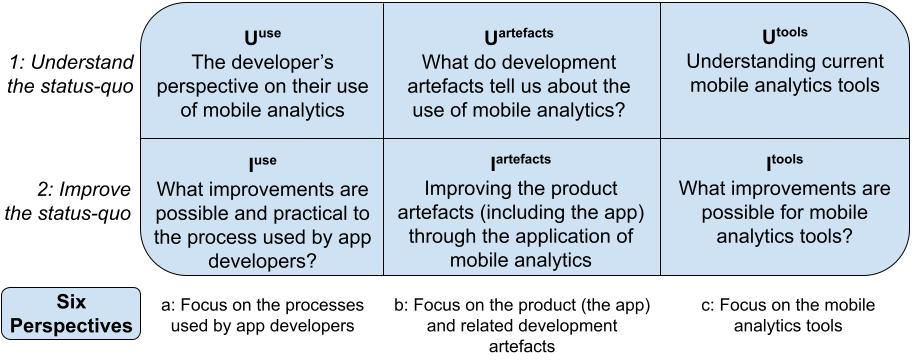
\includegraphics[width=\linewidth]{images/my/six-perspectives-2x3-matrix-12-nov-2021.jpeg}
    \caption{Methodology six perspectives (repeated)}
    \label{fig:six-perspectives-in-the-methodology}
\end{figure*}

The research is both \emph{knowledge-seeking} and \emph{solution-seeking} in nature~\sidecite[][p. 11-4]{stol2018_the_abc_of_software_engineering_research}. Knowledge-seeking in terms of understanding the use of mobile analytics in the practices, development artefacts, and in understanding the mobile analytics tools that are being used. And solution-seeking in terms of considering improvements to each of these three objects of analysis.

\section{Evidence requirements}~\label{methodology-evidence-requirements}
Answering the research question requires rich, contextualised evidence of how developers use mobile analytics in practice. Hutchins writes about studying `cognition in the wild' to provide rich and emergent findings from the real world for phenomena that are hard to capture and analyse without their rich context
~\sidecite{hutchins1995_cognition_in_the_wild}.
Hence, the research needs to be situated in real-world industry practice and experience, drawing on different examples of real-world apps and projects for which analytics have relevance, \textit{i.e.}, that are part of an app-store ecosystem that collects analytics, and that are used by real-world users. 

A comprehensive statistically representative sample of mobile apps was beyond the scope (and feasibility) of a PhD. Instead, this research adopts the approach of `purposive sampling'  as described by ~\sidecite[][pp. 180-182]{flick2018_an_introduction_to_qualitative_research_sixth_ed}. \marginnote{Flick uses the term `purposive sampling' which is treated as a synonym of purposeful sampling in this thesis}. A similar approach has been applied successfully by other researchers undertaking in-depth, qualitative explorations of software development practice, e.g., recent work on qualitative analysis of pair programming undertaken by Zieris who observed~\emph{``Unlike for quantitative methods, statistical generalization from a sample to the population is not a goal. Instead, qualitative studies look for information-rich cases that allow to deepen the researcher’s understanding. Early in the process, each case is treated as unique and studied in great detail; cross-case analyses follow later and are based on the well-understood individual cases.''}~\sidecite[][p.114]{zieris2020_phd_qualitative_analysis_of_knowledge_transfer_in_pair_programming}. 

Flick presents six strategies of purposive sampling [p. 181]. Of necessity the sample used by this research was opportunistic -- what Flick described as ``convenience'' sampling. As Flick notes wryly: \emph{``the problem of access may be one of the crucial barriers''}[p. 182], which applies particularly when seeking access to sensitive data and information about software failures for commercial mobile apps. Nevertheless, the research strove to use a variety of projects and apps including: commercial and volunteer-led development teams; solo developer; small, medium and large development teams; industry and opensource apps; apps that include in-app mobile analytics and those that choose not to. Some of the projects that declined to participate in the research would have helped address some of the gaps in coverage of the known varieties of projects and apps.

Further, the research explored a variety of analytics tools, as no two are identical: they offer a variety of features and capabilities, and have distinct behaviours.  Furthermore there are tools that work at the platform level and others that work at the app level; researching tools that work at both levels helps determine and distinguish their characteristics and compare their behaviours. There is only one platform-level mobile analytics tool in Google Play, the one that Google provides. In contrast, there are tens of app-level mobile analytics tools, so there is value in studying several these app-level mobile analytics tools.

The varieties of projects, apps, and mobile analytics tools, are all intended to help to uncover emergent features, capabilities, and behaviours; they also help establish ranges of examples of improvements and concerns. An additional objective is to increase the `weight of evidence' in support of particular propositions, rather than to prove them~\sidecite[][see p. 569]{seaman1999_qualitative_methods_in_esse}, which is impractical in the scope of this research.


\section{Data sources}~\label{methodology-data-sources}
The nature of research in a sometimes messy real-world environment means access is opportunistic and often occasional. The evidence will be incomplete, yet rich, complex, and multi-faceted because of the variety of projects investigated. For this research the data sources include:

\begin{itemize}
    \itemsep0em
    \item \textbf{\Gls{glossary-development-artefacts}}: their origin is the development team. They include: app binaries, app source code, tests, work schedules, documentation, bug tracking systems, \textit{etc.}, these were collected during the various case studies and complemented by public sources for additional mobile apps. 
    \item \textbf{\Gls{glossary-grey-material}}: Some examples were gathered during the case studies; others were found during additional background research.
    \begin{itemize}
                \item Grey data\index{Grey data} includes: various discussion forums used by mobile app developers and other online contextual information, online issue tracking and related code for opensource projects beyond those that were the focus of the app-centric case studies (\textit{e.g.}, open source networking libraries used by Android apps). 
                \item Grey literature\index{Grey literature} includes: online materials on mobile analytics tools, articles including on medium.com and various blogs. Some were found in response to observations during particular case studies, others were found during additional background research.
    \end{itemize}
    \item \textbf{Pre-study interviews}: with developers and, as appropriate, authorised representatives of their organisation. These were used for setting up the study and understanding the development context. They were collected as part of the case studies.
    \item \textbf{Mid-study communications with developers}: usually email correspondence for clarification, to obtain updates, or comment on observations. These were collected as part of the case studies.
    \item \textbf{Field notes}: some handwritten, others recorded as text on computers. These were collected as part of the case studies and during background research.
    \item \textbf{Analytics tools and associated analytics artefacts}: their origin is the mobile analytics tool. Analytics artefacts, in particular, were a key data source; they include various outputs including screen captures, screen-scraping and parsing, results from calling APIs, and automated emails generated by analytics tools. Product documentation, online help materials, examples, and so on were also used. For open source analytics tools, the code was also used as a data source. All these data sources were collected on an ongoing basis during case studies and during additional background research.
\end{itemize}

The evidence is based mainly in real-world cases, augmented with micro-experiments where these were more appropriate. For all of these real-world cases, collection of naturally-occurring data (\textit{e.g.}, development artefacts, grey material) was augmented by elicitation of additional data (\textit{e.g.}, interviews and communications with developers) to provide clarification, breadth and insight.  Different research methods made use of these data sources, as appropriate.

In terms of the methodology, during the case study it is vital to collect and perform ongoing analysis of mobile analytics and whatever other materials are available. Many of these are ephemeral in nature. For instance, graphs generated by analytics tools may change by the minute. There is seldom a manual for the mobile analytics outputs (\textit{e.g.}, the reports). Furthermore, many of the reports are dependent on the underlying data and/or on changes in the underlying service; therefore the researcher often needs to learn the mobile analytics reporting iteratively in an exploratory manner. For example, one of the findings, reported in \secref{tata-runtime-encapsulation-of-errors}, was the runtime encapsulation of crashes in the application code. This was discovered through one of the app-centric case studies and corroborated by a second one, and then also through grey data. They were not documented \emph{a priori}. 


Third-party mobile analytics (including those provided by Google) have terms of use. These terms of use have various names, such as a policy, \textit{e.g.} for Google Play ~\sidecite{google_play_developer_policy_center}. These may place limitations on data collection and use of the relevant service. For the research covered in this thesis, data collection used a conservative approach to reduce the risk of consequential issues for the researcher, the project, and the stakeholders for the app. This topic and the implications are expanded on in the Discussion chapter in Section~\secref{discussion-on-methodology-and-case-study-procedure}, starting on page~\pageref{discussion-on-methodology-and-case-study-procedure}.

The choice of tools, including the humble web browser used by the researcher, affects aspects of the ease of collection of online reports. As an example, the screenshot capability of the Mozilla Firefox browser~\sidenote{Described in \url{https://screenshots.firefox.com/}} is far richer than that provided by Google Chrome\index{Google Chrome} at the time of writing. Many of the reports in mobile analytics tools require extensive vertical scrolling; Firefox\index{Firebox} can capture the entire contents easily, but Chrome does not. 

Similarly some content is only generated on screen on demand, in response to user actions, for example through scrolling vertically (such as using `infinite scrolling'~\sidecite[]{parker2012_infinite_scrolling}) and/or paging through reports. Others are contextual and may only appear when the relevant conditions occur. For example, the release management reports in Google Play Console appear for the first 7 days of a new release. 

Therefore, to capture the content the researcher (or a human/automated proxy) needs to perform these actions and to save/safeguard pertinent materials to facilitate longer term analysis and provide/record evidence. Where practical, the underlying text was collected in addition to visual content; we created software called \myindex{Vitals Scraper} do so for Google Play Console with \myindex{Android Vitals}. The text could then be processed relatively easily and without needing to be re-keyed. Note: it is not always practical or useful to record ``everything"; how much is suitable is a topic for future research. 

\subsection{Mapping the data sources to the six perspectives}
The various data sources described in the previous section each contribute to the six perspectives as indicated in Table~\ref{tab:mapping-datasources-to-six-perspectives}. The table has two indications of the strength of the contribution: `\textbf{S}' indicates a strong contribution, and `\textbf{m}' indicates a moderate contribution. The blank cells indicate low, or marginal, contributions rather than necessarily no contribution at all.

\begin{table*}
    \small
    \setlength{\tabcolsep}{4pt} %% default is 6pt
    \setlength{\arrayrulewidth}{0.1mm}
    \centering
    \begin{tabular}{l|ccc|ccc}
      & \multicolumn{3}{c|}{\bfseries \small Understand} & \multicolumn{3}{c}{\bfseries \small Improve} \\
      \toprule
         % &\textsubscript{u}Use &\textsubscript{u}Artefacts &\textsubscript{u}Tools &\textsubscript{i}Use &\textsubscript{i}Artefacts &\textsubscript{i}Tools \\
         \multicolumn{1}{r|}{Six perspectives} &\uuse &\uartefacts &\utools &\iuse &\iartefacts &\itools \\ % Thanks to https://tex.stackexchange.com/a/33488/88466
        \hline 
        Development artefacts                       &S &S &m &m &m &m \\
        Grey Data                                   &S &m &m &  &  &  \\
        Grey Literature                             &m &m &m &m &m &m \\
        Pre-study interviews                        &S &  &m &m &m &m \\
        Mid-study communications with developers    &m &m &m &m &m &m \\
        Field notes                                 &S &m &S &S &S &S \\
        Analytics tools \& their artefacts          &m &m &S &m &S &S \\
        \bottomrule
    \end{tabular}
    \caption[Mapping data source (rows) to the 6 perspectives (columns)]{Mapping data source (rows) to the 6 perspectives (columns) \\ S = \textbf{S}trong contribution \\ m = \textbf{m}oderate contribution}
    \label{tab:mapping-datasources-to-six-perspectives}
\end{table*}

\Gls{glossary-development-artefacts}\index{Development artefacts} contribute strongly to understanding of the use of mobile analytics and the artefacts themselves. They also contribute to the understanding of mobile analytics tools, for instance as they contain the usage of any API's provided by a mobile analytics tool. Through understanding the development artefacts, various potential improvements emerge for each of the three objects of analysis.

Grey data\index{Grey data}, \textit{e.g.} developer-centric discussions in project issues on GitHub and Q \& A on StackOverflow, contribute mainly to understanding the current state of affairs, both the immediate issues and historical issues that may or may not have been addressed or retired through changes to the mobile analytics tools and any of their associated SDKs. While they may also hint at future improvements, that's seldom the focus of the developer-centric discussions, although occasionally external developers may also suggest and/or contribute specific improvements.

Grey literature\index{Grey literature} can contribute moderately to all six perspectives, limited partly because the material tends to be general in nature rather than specific to particular apps or projects.

Pre-study interviews contribute mainly to understanding a team's current use of mobile analytics tools. They seldom get into detail about the development artefacts, apart from various statistics that are reported by mobile analytics tools, \textit{e.g.}, the crash rate of the team's app(s). They often indicate areas of improvement across the board that the team could make, but not in enough detail to provide concrete improvements at this early stage in the relationship.

Mid-study communications are often focused on understanding immediate and recent events from a variety of sources (including use, changes to the artefacts, outputs from the mobile analytics). During discussions that are part of the communications, scope for improvements emerge across the board.

Field notes may well be the strongest data source overall, the only area where they're limited to a moderate contribution is in terms of understanding the artefacts -- generally the understanding of the artefacts is evidenced primarily in the development artefacts directly, so the field notes augment these rather than being the strongest source of information for \uartefacts.

Perhaps unsurprisingly, analytics tools and associated artefacts contribute most strongly to the use and improvement of the tools themselves. They also contribute strongly to improvements in the artefacts, \textit{e.g.}, through identifying areas in the source code that lead to a crash.


\section{Methodology}~\label{methodology-methodology-section}
The methodology builds on three primary complementary sources: Ball and Ormerod's `cognitive ethnography', Runeson and Höst's `guidelines for conducting and reporting case study research in software engineering', and Seaman's `Qualitative methods in empirical studies of software engineering'~\sidenote{Note: this methodology was also influenced by additional research from a variety of authors in the fields of software engineering and \acrfull{esse}}.

Broadly, this research starts from what Ball and Ormerod described as `cognitive ethnography'~\sidecite{ball2000_putting_ethnography_to_work_cognitive_ethnography}, that is, observation-based enquiry conducted \textit{in situ} to investigate ``...the interplay between people-laden contexts and expert cognition'' [p. 149]. Ball and Ormerod characterise cognitive ethnography in terms of observational specificity, verifiability and purposiveness: 

\begin{quote}
  \textit{``Our own conception of cognitive ethnography is characterized by three key features. First, it relies on small-scale data collection based around representative time slices of situated activity. As such, it demonstrates observational specificity, as opposed to the intensity of a prototypical ethnography. Second, it is purposive, in that its mode of questioning focuses on issues that are informed by some intention to intervene with, or somehow affect, existing work practices ... Third, it places a strong emphasis on verifiability, in terms of validating observations across observers, data sets and methodologies.''}   ~\sidecite[][p.152]{ball2000_putting_ethnography_to_work_cognitive_ethnography} 
\end{quote} %

Consistent with this orientation, this research sought to derive a situated understanding of analytics (in terms of the six perspectives in Figure~\ref{fig:six-perspectives-in-the-methodology}). The insights that emerged from the more ethnographically-inspired analysis of naturally-occurring data were then investigated further and tested using other approaches, namely across-case comparison, hypothesis testing (systematic manipulation in micro experiments) and action research (evaluation through interventions in specific cases) -- consistent with Ball and Ormerod's emphasis on verifiability.

As Runeson and Höst note, software engineering motivates specialised research methodologies as the study objects: are 1) organisations who \emph{develop} software, 2) the work is project-oriented, and 3) the work is advanced engineering work by highly educated people~\sidecite[][pp. 132-133]{runeson_2008_guidelines_for_conducting_and_reporting_case_study_research_in_sw_eng}. % See below comment for the relevant text.
These criteria apply to all the case studies in this research, and therefore a variety of research methods was adopted in order to perform the research effectively and productively. 

\begin{comment}
The study objects are 1) private corporations or units of public agencies developing software rather than public agencies or private corporations using software systems; 2) project oriented rather than line or function oriented; and 3) the studied work is advanced engineering work conducted by highly educated people rather than routine work. 
\end{comment}

My research is situated in development teams that create mobile apps and use software tools -- in particular mobile analytics -- in order to provide apps that work adequately for their userbases. As Seaman notes, it's important to study \emph{``nontechnical issues and the intersection between the technical and nontechnical in software engineering''}~\sidecite[][p. 557]{seaman1999_qualitative_methods_in_esse}. Seaman notes further that the key advantage of using qualitative methods is to force the researcher \emph{``to delve into the complexity of the problem rather than abstract it away."} [p. 557].

\begin{figure}
    \centering
    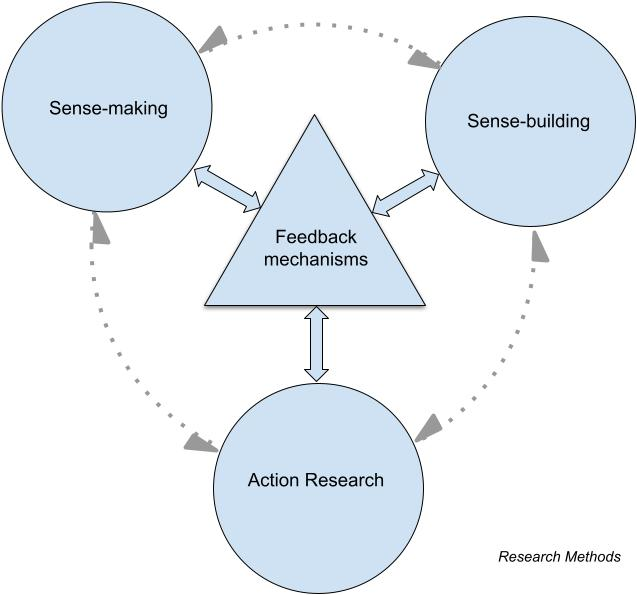
\includegraphics{images/my/categories-of-research-methods-02-aug-2022.jpeg}
    \caption[Categories of research methods]{Categories of research methods \\Source for the figure: {\footnotesize \href{https://docs.google.com/drawings/d/1DpnrvH1ajAKtmcpbJjTWEshdQG_nAIfDS_eAL8obSAQ/edit?usp=sharing}{Google Drawing: Research Methods in PhD}}}
    \label{fig:categories-of-research-methods}
\end{figure}


\subsection{Categories of research methods}
Figure~\ref{fig:categories-of-research-methods}, on page~\pageref{fig:categories-of-research-methods}, provides a visual overview of the four categories of research methods used to serve this `cognitive ethnography' approach; they include 1) sense-making, 2) sense-building, and 3) evaluation through action research, which were complemented by the fourth category 4) feedback mechanisms to help support and verify the analyses. 

Note: Figure~\ref{fig:categories-of-research-methods} is an over-simplification with clear boundaries between the categories in order to convey the alignment of methods to purposes, and the categories are not discrete.  Some methods include several data sources, and some data sources are analysed using several methods. In practice, individual research methods provided multi-faceted contributions; for instance local app experiments contributed to both sense-building and sense-making. 

Table~\ref{tab:mapping-analysis-to-six-perspectives} identifies the various research methods, groups them in terms of their roles in the research (as illustrated in Figure~\ref{fig:categories-of-research-methods}), and maps them to the six perspectives.  Each of these research methods includes data collection \textit{and} analysis unless otherwise stated.


\begin{table*}
    \small
    \setlength{\tabcolsep}{4pt} %% default is 6pt
    \setlength{\arrayrulewidth}{0.1mm}
    \centering
    \begin{tabular}{l|ccc|ccc}
      & \multicolumn{3}{c|}{\bfseries \small Understand} & \multicolumn{3}{c}{\bfseries \small Improve} \\
      \toprule
         % &\textsubscript{u}Use &\textsubscript{u}Artefacts &\textsubscript{u}Tools &\textsubscript{i}Use &\textsubscript{i}Artefacts &\textsubscript{i}Tools \\
         \multicolumn{1}{r|}{Six perspectives} &\uuse &\uartefacts &\utools &\iuse &\iartefacts &\itools \\ % Thanks to https://tex.stackexchange.com/a/33488/88466
         
        \hline 
        \textbf{Sense-making} & & & & & & \\
        (comprehension and exploration) & & & & & & \\
        Beacon finding and    &S &m &S &m &m &m \\
        Drill-down            &m &m &S &S &m &m \\
        %\tabucline[1pt on 3pt]  \\ % See https://tex.stackexchange.com/a/109301/88466 however here it is terminated prematurely and a bit heavy 
        % Or try https://tex.stackexchange.com/a/229334/88466 or https://tex.stackexchange.com/a/613907/88466 if I've not collapsed these two previous rows soon.
        % Or use a newer latex package, see https://tex.stackexchange.com/a/611494/88466 

        \hline
        \textbf{Sense-building} & & & & & & \\      
        %(Integration and differentiation)    & & & & & & \\        
        (micro-experiments and macro-discoveries) & & & & & & \\
        Local App Experiments   &m &S &S &  &S &S \\
        FOSS Analytics Experiments      &  &  &S &  &  &S \\
        Across Case Comparisons &S &m &S &S &m &m \\        
        
        \hline
        \textbf{Feedback mechanisms} & & & & & & \\
        (triangulation and validation) & & & & & & \\
        Ask The App Devs      &S &m &m &m &m &m \\
        Ask The Tool Devs     &  &  &S &m &m &m \\
        Grey Literature \& Grey Data Analysis       &m &m &S &m &m &  \\
        Code, \& app-binary, Analysis         &m &S &  &m &m &  \\
                
        \hline
        \textbf{Action research} & & & & & & \\
        (embedded intervention)  & & & & & &  \\
        Observation and Analysis &S &S &S &S &S &m \\
        Field Experiment         &m &  &  &S &S &  \\
        Hackathon                &m &m &  &S &S &  \\
        
        \bottomrule
    \end{tabular}
    \caption[Mapping research methods (rows) to the 6 perspectives (columns)]{Mapping research methods (rows) to the 6 perspectives (columns) \\ S = \textbf{S}trong contribution \\ m = \textbf{m}oderate contribution \\FOSS = Free and Open Source Software}
    \label{tab:mapping-analysis-to-six-perspectives}
\end{table*}

`\textbf{Sense-making}'\index{Sense-making} methods were concerned with understanding current practice (as reflected in artefacts, tools, and developers' practices and perspectives -- i.e., perspectives \uartefacts, \utools, and \uuse) and identifying potential improvements in tools and in how analytics are used in app development and maintenance (i.e., perspectives \itools and \iartefacts). The research methods include beacon-finding (see page~\pageref{section-beacon-finding-method}) and drill-down (see page~\pageref{drill-down-research-method}).

Sense-making incorporates an iterative pattern of \textbf{beacon finding} to identify areas of interest within a case, \textbf{drill-down} to investigate one or more beacons, and comparisons both within and across~\footnote{While across-case comparisons are grouped under sense-building, they also help with sense-making.} cases to identify patterns, relationships, counterfactuals~\footnote{\emph{``...relating to or expressing what has not happened or is not the case." Oxford Languages.}}, as some characteristics emerge in contrasts across and between studies. Comparisons were performed iteratively on an ongoing basis (for active apps the values are not constant). These comparisons included comparisons across releases, using different windows of time, on different dates, comparisons with peers, and so on.


`\textbf{Sense-building}'\index{Sense-building} methods build on -- and test -- insights found through sense-making. The research methods included micro-experiments, carried out on local apps (see page~\pageref{local-app-experiments-research-method}), FOSS analytics experiments % COULD-DO Arosha's suggested alternative concepts of white and black box testing of the tools. I'm mulling these over. TBD.} 
(see page~\pageref{foss-contributions-research-methods}), and across-case comparisons (see page~\pageref{across-case-comparisons-research-method}).

Local app experiments\index{Local app experiments} (see page~\pageref{local-app-experiments-research-method}) were used to investigate detail and give insight into the relationships between tools, quality of analytics, and potential impact of analytics use on apps (i.e., perspectives \uartefacts, \utools, \iartefacts, \itools).

Across-case comparisons\index{Across-case comparisons} (see page~\pageref{across-case-comparisons-research-method}) identify macro-discoveries -- that is, they identify characteristics and patterns that were not evident in individual case studies, potential improvements to practice (i.e., perspectives \uuse and \iuse), as well as the influence of the quality of tools in practice (\itools). They can also corroborate and/or challenge findings found in individual cases.


`\textbf{Feedback mechanisms}'\index{Feedback mechanisms} were used to support and verify the other analyses, by comparing observations to other evidence, or by asking developers for clarifications or reflections. Feedback mechanisms were used throughout the research and contributed mainly to the understanding of perspectives associated with (\uuse, \uartefacts, and \utools); nonetheless they were also used frequently when considering improvements (\iuse, \iartefacts, and \itools). 

`\textbf{Action research}'\index{Action research} methods were concerned largely with understanding the use of analytics in context and the evaluation of the effect of improvements in the use of analytics, in terms of adoption into use and app performance (i.e., perspectives \iuse and \iartefacts). It includes three research methods: 1) observation and analysis, 2) field experiment, and 3) hackathon. These are explained on page \pageref{section-action-research-method} onward. 

The research was iterative, moving through sense-making, sense-building and feedback mechanisms repeatedly as new cases were studied or new insights emerged.  The methods and the data sources often also informed several of the six perspectives.  These research methods are introduced in more detail in the sections that follow.

\subsection{Sense-making}\index{Sense-making}
% c.f. https://en.wikipedia.org/wiki/Sensemaking_(information_science)
%1) Identifying patterns (inductive analysis) c.f. grounded theory. 2) 

`Sense-making' focuses on understanding the current practices and identifying potential improvements in practices and tools.  It includes beacon finding (inductive analysis of different forms of data to identify areas of interest) and drilling down (further data collection and analysis to understand those areas of interest in context). Sense-making can include other activities, such as:
 
% NB: I'm not quite sure where to place the following, I might end up moving it or splitting it apart into various sections.
 \begin{itemize}
    \itemsep0em
    \item Collating similar failures.
    \item Ordering and ranking clusters of failures.
    \item Bug identification and localisation: Establishing potentially pertinent patterns in the reports, and characterising when a failure \emph{does and does not} occur are part of this work. Obtaining an identifying definitive boundaries may be impractical, the work is often iterative and exploratory in nature and lossy. 
    \item Bug investigation.
    \item Checking whether there is likely to be sufficient evidence for any triage process.
\end{itemize}

\begin{figure}
    \centering
    \includegraphics[width=6cm]{images/my/Boston-matrix-app-and-mobile-analytics-tool.jpeg}
    \caption{Boston matrix for app and mobile analytics tool}
    \label{fig:boston-matrix-app-and-mobile-analytics-tool}
\end{figure}

\subsubsection{Beacon-finding}~\label{section-beacon-finding-method}\index{Beacon-finding}

The notion of \textbf{`beacons'} is borrowed from research on program comprehension; for instance by Wiedenbeck, who helped establish the notion of beacons in software development: ~\emph{``In programming, beacons are lines of code which serve as typical indicators of a particular structure or operation''}~\sidecite[][p. 679]{WIEDENBECK1986_beacons_in_computer_program_comprehension}. The work was extended and updated to explicitly consider the effects of beacons in comprehension of source code, for instance in~\sidecite{crosby2002_roles_beacons_play_in_comprehension_etc}.

The notion of beacons was generalised for this research to include indicators in the analytics of something of interest, or something that required attention.  And so `beacon finding' was an inductive process by which significant indicators in the analytics data were identified -- and then used to identify areas of the code base that required further investigation.  Mobile analytics may include source code that calls APIs in the application's source code, however the bulk of the contents that need to be comprehended comes as outputs from the mobile analytics tools, therefore the beacons will differ accordingly. In this research the beacons include: the shape of graphs in mobile analytics report, failure clusters, a method call in stack traces, and so on.

%\marian{Now specify how you spotted beacons... I looked for things on this basis, how I kept track of things, what selection criteria were used and why?}

\begin{kaobox}[frametitle=Beacons in Mobile Analytics]
\section{Beacons in Mobile Analytics}
\textit{This is where I'll gather notes on beacons found in mobile analytics outputs. It may eventually be incorporated into my thesis. For now, it's where raw content and ideas will be collected and later collated.}

Inspirations include:
\begin{itemize}
    \item Scott Barber's work on modelling software performance [testing].
\end{itemize}

Candidates for beacons include (numbered for ease of reference):
\begin{enumerate}
    \item An aggregate increase in error rate
    \item Early adverse trends during a phased release rollout
    \item Correlations with one to a few predetermined factors (e.g. OS release, device model, ...)
    \item 
\end{enumerate}
\end{kaobox}

Beacons emerge in various ways. For instance in reports they include: anomalies within a report, mismatches and inconsistencies between two sibling reports or between a master report and the linked detailed report%~\todo{Arosha, suggested introducing these terms for different types of report when discussing analytics tools in the lit. review. I agree, TBD once the lit. review has been reworked.}
, in the shape of the curve of a graph, in the distribution and groupings of aggregate data, and so on. Similarly, alerts as determined by a mobile analytics service may be considered potential beacons being `promoted' by the mobile analytics reports. 

The most common method of recording potential beacons in this research was using web browser screenshots and/or other mechanisms that preserved information electronically. Some were annotated as part of the beacon-finding and drill-down analysis. Additional notes were written both electronically and/or in physical notebooks. 

Selection criteria included: top ranking results, atypical rates of change, adverse changes to reliability, novel failures particularly for the most recent release, etc. A consistent and overriding criterion was to seek beacons that indicated flaws and failures that could materially and adversely affect the user experience of the app for one or more users of the app.

\subsubsection{Drill-down}~\label{drill-down-research-method}
Beacons identify areas of interest; these need to be investigated further by `drilling down' and examining the underlying information sources. For example:  Is the identified beacon genuinely significant? Does it generalise to other contexts?  What does it signify or relate to in the app and its usage, etc.?  Drill-down starts with the original data sources, but may draw in other data sources to clarify relationships, responses by the developers, etc. 

For Segment 1 of Figure \ref{fig:boston-matrix-app-and-mobile-analytics-tool} (\emph{i.e.} the same app and the same mobile analytics tool) examples include:

\begin{itemize}
    \itemsep0em
    \item Going into greater detail in the current report for a `failure cluster'\index{Failure cluster} to understand its characteristics.
    \item  Investigating in more detail in order to understand the report, the nature of the problem, the causes, and effects. 
\end{itemize}

For Segment 3 (\emph{i.e.} a different app using the same analytics tool) examples include: 

\begin{itemize}
    \item Looking across apps to see if the same and/or similar failures were happening in any of those other apps.
    \item Looking at the characteristics of the failures in the various apps, for instance does a failure happen as often? on the same release of the operating system? on the same device models? and so on.
\end{itemize}

For Segment 2 (\emph{i.e.} the same app using other analytics tools):

\begin{itemize}
    \item Does the same failure appear in all the analytics tools, and if so, are the characteristics similar or do they differ in particular ways?
\end{itemize}

Segment 4 (different apps \emph{and} different tools) did occur sometimes in the case studies, however these are beyond the scope of this research \emph{e.g.} as one of the apps was a web app.

The drill-down may be expanded further using feedback mechanisms, e.g.:
 
\begin{itemize}
\itemsep0em
\item Searching grey data\index{Grey data} and grey literature\index{Grey literature} and cross-referencing of materials.
    \item Asking people: for instance colleagues, the developers of the app, the developers of the mobile analytics tool, \textit{etc}.
    \item Check development artefacts as these may provide relevant and pertinent information and clues.
\end{itemize}

A representative example of using the feedback mechanisms is:

\begin{itemize}
    \item A new release of one of the apps resulted in a five-fold spike in the crash rate for the new release. After drilling-down into both the platform and the in-app analytics, the source code of the network library was reviewed in tandem with searching for similar issues reported on StackOverflow. These helped with identifying the epicentre of the crashes.
    \item Automated tests for the network library were then used as a basis for devising similar tests for the app. These tests reproduced the crash and demonstrated the subsequent changes to the app were effective in fixing the crash.
    \item And when the modified app was released the mobile analytics confirmed the spike had been successfully addressed in the new release.
\end{itemize}

This example served both the research needs and the practical project needs; and it transpires that developers use a similar form of sense-making; this is discussed in \secref{aiu-sensemaking-and-decision-taking-by-developers-section}, starting on page \pageref{aiu-sensemaking-and-decision-taking-by-developers-section}.

\subsection{Sense-building}
Sense-building moves beyond sense-making. Sense-making aims to understand \textit{what is}, while sense-building extends sense-making with direct action and more active research, for example: to devise and run experiments to learn more about the behaviours of mobile analytics, and to seek patterns and generalisations across tools, and case studies. The main methods used for sense-building were local-app experiments, experimentation with \Gls{foss} analytics tools and across-case comparisons. 

\subsubsection{Local-app experiments}~\label{local-app-experiments-research-method} 
\textbf{Local app experiments}\index{Local app experiments} were used to \textit{test the understanding} of the relationships between the usage and the analytics through manipulations of apps and observation of the effects -- hence, the local app experiments were used to test some of the patterns identified in the inductive analysis. They consist of \textit{micro-experiments}\index{Micro experiments} involved creating and developing small mobile apps intended to exercise particular aspects of mobile analytics~\marginnote{Similar to the `invent the future' adage, for example: \href{https://quoteinvestigator.com/2012/09/27/invent-the-future/}{quoteinvestigator.com/2012/09/27/invent-the-future/}}). The inputs to an app were directed in order to determine the outputs from mobile analytics. This was essentially a form of black-box test, where the analytics tool being studied was the system under test \acrfull{sut}\index{System under test (SUT)}. These micro-experiments helped to answer questions and gaps observed as part of sense-making\index{Sense-making}.  In particular, they provided insights into the relationships between tools, quality of analytics, and potential impact of analytics use on apps (i.e., perspectives \uartefacts, \utools, \iartefacts, \itools). 

The apps that were developed as local-app experiments are small mobile apps and not intended for production use. They were developed in order to investigate the relationships between the inputs (such as usage) and the analytics outputs (such as reports) through deliberate manipulation of the inputs and observation of the consequences.  

The local-app experiments allow for tighter control on the usage, \textit{i.e.}, the inputs, in comparison to the unfettered use of real-world mobile apps. They can help surface behaviours and provide for tighter evaluation in the early, pre-launch/pre-production phases. %I can't say feedback as that'd conflate the other use of feedback here in the methodology.
The local app experiments were used to test some of the patterns identified in the inductive `sensemaking' analysis.

Where practical the source code of these apps is made available under a permissive opensource license to facilitate further research by others and in order to facilitate inspection by and feedback from others.

%\akb{Also explain how the results of these experiments connected to other parts of the method? e.g., did they change / add to the sense-making activities?}
The results of the local app experiments helped augment the across-case experiments, particularly in terms of providing additional results to compare with those from the app case studies. They also informed discussions with the app and tool developers. 

\subsubsection{FOSS analytics experiments}~\label{foss-contributions-research-methods}
The research carried out experiments on several \acrshort{foss} analytics tools to gather evidence on how these tools worked. Additionally, these experiments explored the processes used by the relevant \acrshort{foss} projects to accept and adopt contributions that aimed to improve one or more elements of the respective codebase and thereby improve the respective analytics product offering.

As the research had access to the source code of the tools studied, the investigation of how these analytics tools worked can be considered to be a form of white box testing, where simple apps were used as test drivers to exercise the functionality of the analytics components. The exploration of the project processes for adopting changes were more like grey box tests as there was only partial visibility of the dynamics of the relevant project teams. 
The \acrshort{foss} analytics experiments were relatively small in scope and made on an \emph{ad-hoc} rather than a systematic basis~\sidenote{While systematic contributions may be a valid approach to research this topic, it was not core to this research.}.%~\todo{Add table listing analytics tools studied and whether they were subject to black box, white box or grey box testing}

\subsubsection{Across-case comparisons}~\label{across-case-comparisons-research-method}
\textit{Across-case comparisons} were concerned largely with understanding current practice and identifying potential improvements to practice (i.e., perspectives \uuse and \iuse), as well as the influence of the quality of tools in practice (\itools). This method draws on the approach discussed in \sidecite[][pp. 567-569]{seaman1999_qualitative_methods_in_esse}, \textit{e.g.}, to compare pairs of case studies to determine variations and similarities, with the additional considerations of seeking areas of potential improvements based on findings from the various case studies.

Similar to using various software testing techniques to find bugs, making comparisons across the case studies can help to identify more of the behaviours of mobile analytics, their use, and their efficacy. Across-case comparisons can increase the probability of seeing fresh characteristics and establish similarities across cases. The comparisons across case studies help establish norms (which can also be used to identify beacons, and anomalies), patterns (and anti-patterns), variety, and ranges. 

Comparison across cases (\textit{i.e.}, across projects and their mobile apps) helps both researchers and developers, albeit their interests and focus may differ.

\begin{itemize}
    \item \textbf{For developers}: they can compare the reports for their apps with the results others obtain. Doing so may help them identify problems-in-common (shared problems) and fixes-in-common that work for many apps with similar failures. They can also establish norms and the comparisons help provide triangulation and perspective. Some developers also find peer-group comparisons stimulating.
    
    \item \textbf{For researchers}: across case comparisons include `plus one'~\sidecite[][pp. 28-29]{aurini2016_how_to_of_qualitative_research} research that can help uncover emergent behaviour, reinforce existing findings, and so on. The across case comparisons also provide additional microcosms where new findings are discovered in the behaviours of apps, the tools, the development practices, and the efficacy of the use of mobile analytics performed by a wider variety of development teams.
\end{itemize}


The data and the system state for individual apps can help to increase the `coverage criteria' for a mobile analytics tool (which may be considered a system or simply a `box' as in black-box, grey-box, or white-box system)%~\todo{In the planned Tools chapter I can discuss this property of the various Mobile Analytics tools.}. 

We know from a related domain, software testing, that more test cases can increase the detection rate of behaviours. For example, a paper by~\sidecite{briand2007_a_critical_analysis_of_empirical_research_in_software_testing} discusses concepts including the concept of a cost-effectiveness curve and of what the author terms `random variations' and the effect these random variations have on fault detection effectiveness in page 5 of their paper. The set of inputs (\textit{e.g.}, crash reports) into a mobile analytics tool may result in various beacons -- and related data -- appearing in the outputs. By increasing the sets of inputs, particularly from dissimilar apps, there is the potential to increase the appearance of beacons. And the larger volume of beacons across the projects allows for weightier analysis.

A key observation is that detection is not static nor a one-off value; behaviours come and go, particularly in mobile analytics tools where reports are often ephemeral. The value of across-case comparisons increases when the sampling increases to record more of the ephemeral behaviours and outputs.

The nature of this PhD research based on a relatively small number of apps and associated case studies means it is premature to attempt to systematically plot the number of cases against the behaviours that were observed. Instead the focus is on monitoring 
new insights vs. resonance, and how often a new case highlights something that was not noticed in previous ones, even though they were there. % Note I don't have distinct records of when this occurred although it would have done so on many occasions.

\begin{kaobox}[frametitle=Parallels from Software Testing]
\textit{c.f.} Testing and Noticing, by~\textcite{bolton2009_testing_and_noticing}, which discusses noticing (and not noticing) from a software testing perspective.
\end{kaobox}


\subsection{Feedback mechanisms}~\label{methodology-feedback-mechanisms-topic}\index{Feedback mechanisms}
Sense-making and sense-building methods are centred on the research and driven by the researcher's focus and perspective. Unaided -- even if they are productive -- they risk being marginalised and disconnected from the work of others, in particular the work of those who actually develop the apps and the tools. 

This research used four `feedback mechanisms' to validate and challenge the research outputs of sense-making and sense-building:

\begin{itemize}
\itemsep0em
\item ask the app developers
\item ask the tool developers
\item analysis of grey literature and grey data
\item analysis of code
\end{itemize}

The first two (i.e., the mid-study communications with developers) extend understanding of topics emerging from sense-making or sense-building, consistent with Ball and Ormerod's `cognitive ethnography'~\sidecite{ball2000_putting_ethnography_to_work_cognitive_ethnography} and Petre's `targeted observation'~\sidecite[][p.234]{petre2009_insights_from_expert_software_design_practice}, by engaging with the developers who are situated in their actual practice in their real-world microcosm.  For example, the developers can be asked about their experiences, perceptions or reasoning about emergent observations, or to explain particular decisions or practices that have been highlighted by the research. The latter two feedback mechanisms provide comparison to additional data drawn from analysis of existing information (i.e., grey literature\index{Grey literature}, grey data\index{Grey data}, code).  The feedback mechanisms draw on multiple data sources, including some which are independent of the research, hence allowing for comparison/triangulation/colligation -- all with a focus on the research questions.

\subsubsection{Ask the app devs}~\label{section-ask-the-app-devs-research-method}\index{Ask the app developers method}
The developers of the apps are uniquely able to voice their perceptions and thinking on their use, experience, and perceptions of using mobile analytics. They are therefore well placed to provide feedback on their use of mobile analytics and also answer questions about their use of mobile analytics in their development artefacts and their perceptions of the mobile analytics tools.

They are also busy with their challenges related to developing and improving the mobile apps they are responsible for. As Petre notes in~\sidecite{petre2009_insights_from_expert_software_design_practice} experts are willing to try/explore many tools; however they focus on what can help them, and they may discount many aspects of the mobile analytics tools including some of the characteristics and behaviours of interest from a research perspective. Nonetheless from a research perspective it may be useful to learn more about why they have discounted or rejected various aspects of the tools. 

\subsubsection{Ask the tool devs}~\label{section-ask-the-tool-devs-research-method}\index{Ask the tool developers method}
The tool developers understand their mobile analytics tools in depth and many have a unique vantage point to observe how their mobile analytics behaves across a large population of apps. Furthermore they are well placed to design, implement, and release fixes and improvements to their mobile analytics products and services. They understand the rationale of their mobile analytics tools and their user-base. And yet, they do not know everything about how their tools are used or perceived and many are keen to receive feedback and insights accordingly.

The research method entails communicating with knowledgeable, available and interested people who develop (in the broad sense) the relevant mobile analytics tool. The communication may be direct or indirect (for instance via their customer service, via online feedback links, or in the form of contributions to their opensource project). Being able to provide succinct, clear, timely, and relevant communications may increase the chances of engaging in a mutually productive dialogue.

\subsubsection{Grey literature and grey data analysis}~\label{section-grey-literature-and-data-analysis-research-method}\index{Analysis!Grey literature}\index{Analysis!Grey data} %\improvement{So two shades of grey? :)}   

A great deal of grey literature\index{Grey literature} and grey data\index{Grey data}~\sidecite[][pp 219-221]{banks2010_blog_posts_and_tweets_the_next_frontier_for_grey_literature} is available online, covering mobile analytics and to errors, problems related to source code and libraries used in real-world mobile apps. The main sources of relevant grey data include Stack Exchange websites frequented by mobile app developers (particularly \href{https://stackoverflow.com/}{stackoverflow.com}) and GitHub. 

Both Stack Exchange and GitHub provide comprehensive and useful search capabilities which help find relevant content, for instances examples where other development teams have found, understood, and addressed particular crashes in their Android app that also apply to the app in the case study.

\href{https://stackoverflow.com/}{stackoverflow.com} provides facilities that encourage meta-data to be provided by users of the site \textit{e.g.}, tags, votes, accepted answer flag, \textit{etc.}, and their search provides facilities to perform searches that use meta-data as well as free text~\sidecite{stackoverflow2021_search_help}.

The nature of GitHub projects provides some inherent structure which can be utilised when performing searches, for example to search issues and pull requests~\sidenote{\href{https://docs.github.com/en/search-github/searching-on-github/searching-issues-and-pull-requests}{docs.github.com/en/search-github/searching-on-github/searching-issues-and-pull-requests}}. 

\begin{kaobox}[frametitle=Inconsistent terms for searches on GitHub]
Note: GitHub uses the term `qualifier' in the online documentation~\sidecite{github2021_searching_code_github_docs}, and the terms `prefix' and `tag' in their online search page \href{https://github.com/search}{github.com/search} to describe their mechanisms to filter the search results. These mechanisms facilitate structured searches of public projects (and others to which the individual has access).
\end{kaobox}


There are similarities in searching programmer-generated grey literature and the low-ceremony evidence described in \sidecite{scaffidi2007_toawards_a_calculus_of_confidence, scaffidi2007developing} where the sources of evidence include votes received by questions and answers on StackExchange sites and on public issue tracking sites including GitHub and Google. % ADD example of Google  

As an example, \href{https://issuetracker.google.com/issues/128796774}{Issue 128796774} in Google's issue tracker reported stack traces in crash reports were unreadable in Android Vitals after the developer switched to deploying their Android app using App Bundles. Two external developers confirmed the issue, as did the Google engineer. Google claims to have fixed the problem, nonetheless the external developers say it was still occurring months later.

The analysis of this type of issue often includes cross-checking between Stack Overflow and Google's Issue Tracker. Sometimes it also includes reviewing issues on GitHub. Where the issue has been seen in one or more of the app-centric case studies potentially there is enough information from these sources to triage the issue for the respective project.

The grey material\index{Grey material} often provides additional examples and/or corroborates issues found in app-centric case studies.

\subsubsection{Code and app-binary analysis}~\label{section-code-analysis-research-method}   

%\unsure{YY: Can you justify to look at grey literature because the academic literature have not covered the research question?} 

Source code provides a snapshot of raw ingredients used by the development team's build process in order to generate an app. Analysis of the binary provides a snapshot of the final result of the build process of the released app.

Source code often includes at least one build `recipe'~\sidenote{For most Android apps the main build recipe is in the file \texttt{./app/build.gradle}.} so the build can also be evaluated and hopefully reproduced~\footnote{Aside from sensitive ingredients such as signing keys used to digitally sign each binary when it is created.}. The source code's repository augments the source code by recording the historical evolution of the source code.

Code analysis in the context of mobile analytics involves searching for indications of the use of one or more in-app mobile analytics libraries in the project's source code~\sidenote{The \Gls{glossary-exodus-privacy-project} \url{https://reports.exodus-privacy.eu.org/en/}\index{Exodus Privacy Project} is one of several tools that can identify the mobile analytics library in an Android application's binary file.}. The steps performed to identify indicators %c.f. beacons as used in this chapter
of the use of a mobile analytics library include:

\begin{enumerate}
    \itemsep 0em
    \item Examine details in one or more \texttt{gradle} scripts where the analytics are added as a `dependency'; the version of the dependency provides useful meta-data on whether the analytics are actively maintained by the developers. % COULD-DO\textit{e.g.} add code snippet e.g. see https://firebase.google.com/docs/analytics/get-started?platform=android#add-sdk
    \item Examine initialisation of the analytics library in the source code; often this occurs in the Android app's \texttt{Application} class. % Ditto there's an example code snippet at https://firebase.google.com/docs/analytics/get-started?platform=android#add-sdk
    \item Examine \texttt{import} statements in individual source code files that reference the analytics Java package(s).
    \item Search for one or more \textit{wrapper} class files. If these exist, then extend the search for these custom classes in step 3 and 5.
    \item Search for calls to the original and any wrapper mobile analytics API classes. % e.g. based on examples including https://firebase.google.com/docs/analytics/get-started?platform=android#start_logging_events
\end{enumerate}

After the five steps have been completed, the matching lines of source code are then available for analysis. 
%
The analysis can be performed for any snapshot of a codebase \textit{i.e.,} for any commit made to the version control repository. Commands such as \texttt{git blame} provide information of the particular commit where lines of code were last updated and complement analysis of the snapshots.

The application of five steps can be scripted. As an example, in joint research~\sidecite{harty2021_logging_practices_with_mobile_analytics} a mix of manual and scripted steps were applied to enable the analysis of the use of Firebase mobile analytics in all the commits made to 57 opensource Android apps.

A useful confirmatory test to help establish the integrity of an app's codebase is to build the app using the build scripts. There may be additional documentation of the build process available, \textit{e.g.}, in a README file incorporated into the code base.

Analysis of the \textbf{app-binary} was limited to free, public, online services, in particular the Exodus Privacy project and AppBrain. Both of these, for different reasons, analyse the binary file(s) for Android apps on Google Play. The Exodus Privacy project focuses on privacy on behalf of end users and identifies the permissions requested by the app and the trackers embedded in the binary file~\sidenote{\href{https://reports.exodus-privacy.eu.org/en/info/understand/}{reports.exodus-privacy.eu.org/en/info/understand/}}; AppBrain focuses on providing information to app developers~\sidenote{\href{https://www.appbrain.com/info/help/index.html}{www.appbrain.com/info/help/index.html}}. In terms of this research, AppBrain provides statistics on the usage of various libraries across the population of apps in Google Play Store; Exodus Privacy provides details of the trackers used in the apps in the app-centric case studies.


\subsection{Action research}~\label{section-action-research-method}
Avison, Lau, Myers, and Nielsen explain the utility and importance of action research in order to establish the relevance of academic research by trying out theories with practitioners in real situations and in real organisations~\sidecite{avison1999_action_research}. They recommend action research \emph{``because this particular qualitative research method is unique in the way it associates research and practice, so research informs practice and practice informs research synergistically."} [p.94]. Action research is particularly relevant for evaluation, when it \emph{``encourages researchers to experiment through intervention and reflect on their intervention and the implication of their theories."} [p.95]. 

This research applies their recommendation where the research informs the practice of both app developers and the work of the developers of mobile analytics tools. Conversely, the research is enriched through understanding the practices and the potential for the application of mobile analytics to help improve the quality of the work of the app developers. The case studies include examples where the researcher's mode of engagement was:
\begin{enumerate}
    \itemsep0em
    \item a consultant and/or an embedded developer: an active participant integrated into the project team;
    \item a coach: of existing teams of app developers who applied the concepts;
    \item an interviewer: of various development teams to learn of their practices and results;
    \item an analyst/observer: performing static analysis of opensource code repositories~\sidenote{Analysis of proprietary code repositories is also possible, but not practicable for this research owing to confidentiality agreements.}.
\end{enumerate}

All the roles support communications with the project and allow the researcher to ask questions, offer suggestions including issues and/or code contributions, and discuss findings with the developers for their case study. All include at least some observation and analysis. 

The coach and embedded developer roles ended up being fairly similar. They both included organising a hackathon and a field experiment for the the Kiwix\index{Kiwix} and Catrobat\index{Catrobat} projects. The material differences were two-fold: a) the embedded developer role continued for several years, whereas the coach role was for several months, and b) the embedded developer role included contributions to the project's code-base.

The consultant role included engineering leadership, mentoring developers and product owners in learning how they could integrate mobile analytics into their work practices, co-writing automated tests and related code, code reviews, and working with various mobile analytics tools throughout the assignment. (Table \ref{tab:app-centric-studies-research-perspective} maps the roles to the app centric case studies.)

\newthought{Engagement:}
The action research was preceded by discussions with the project team (and its organisation) to determine: 

\begin{itemize}
\item what research would be viable and productive; 
\item the role of the researcher; 
\item the depth, scope, range, and duration of the case study; 
\item concerns and constraints that needed to be addressed to protect all the stakeholders involved~\sidenote{The stakeholders may extend beyond the primary participants; for instance, the end users could potentially be stakeholders in what happens during the case study.} while also maintaining the integrity of the research;
\item intellectual property rights, copyright, confidentiality, non-disclosure agreements, and so on~\sidenote{Note: some researchers may be introduced to these together with the ethical aspects under the term LSEPI, discussed in ~\cite{brooke2018__becoming_professional_a_university_perspective}}.
\end{itemize}

The decisions were made mutually by the parties involved. Generally, the project's team and its organisation set the limits and constraints. As \sidecite[][p.324]{barroca_2018_bridging_the_gap} notes, timeliness and relevance are vital to industry partners, while they also want to guard against the research being too intrusive or too demanding of their time or other resources. Therefore, the research needs to offer something of sufficient value, relevance, and timeliness to the project team and its organisation. For example, if they are aware their projects have excessively-high error rates %(for instance if they are aware of these via their mobile analytics reports)
, they may have the motivation to participate in the research in the hope of materially reducing the error rates, and furthermore they may seek an intervention in the guise of action research in order to achieve reductions in any excessively-high error rates.  As the projects generally already have at least one form of mobile analytics, the incremental cost is low in terms of tooling.


\newthought{Wrap-up: }
The wrap-up of a case study included various actions such as safeguarding and archiving evidence; redacting personal details or anonymizing communications with the stakeholders; unsubscribing from services provided for a given case study~\sidenote{Note: the project team may control the researcher's access to various systems and development artefacts, and perform their own equivalent of a wrap-up.}; reviewing findings, analysis, and conclusions with the development teams (and with their organisation); preparing what is appropriate to publish in terms of evidence, and so on. This stage also provided an opportune period for retrospectives of the case study \textit{and} for the research methods and outcomes, while the case study was still topical. 

\subsubsection{Observation and analysis}~\label{section-observation-research-method}
Observation is combined with analysis, both contemporaneous and \emph{post-hoc}.   Findings were presented to the project and development team, in order to: 1) provide value for the team members who were willing to contribute their time and who provided access to their analytics and other artefacts, and 2) encourage scrutiny and validation of the findings and observations.

In this research, observation included either or both development artefacts and analytics artefacts. One example is to observe the outputs from mobile analytics tools (the analytics artefacts) and what the developers do with these subsequently. 

The analysis focused on ways the observations might usefully help the project in terms of improving their development practices and/or their artefacts.

\newthought{Contemporaneous analysis:}
The nature of working with live mobile analytics data and real-world projects means there are likely to be important events that need to be found and processed rapidly in order to preserve their value in terms of the case study. Therefore, one of the success factors in terms of the research is to practice continuous, ongoing, low latency, and iterative analysis, verification, course correction, efficacious communications -- where it is viable to do so~\sidenote{In other words, there are four key tasks: analysis, verification, course correction, and efficacious communications. All of these need to be performed on a continuous, iterative, and ongoing basis. Keep latency in the work to a minimum in order to increase the value of the results and the effects.}. The viability is governed by various factors, including: the working relationships with the project team set in the context of their working practices, research access to the various systems, and the characteristics of the event being reported via the mobile analytics tool(s). 

\newthought{Post-hoc analysis:}
\emph{Post-hoc} analysis is more research-oriented; in contrast analysis during the active case study is often more project-oriented. During the active case studies, there is a need to deal effectively with ephemeral events, data, actions, \textit{etc.} on an opportunistic, often sporadic, basis; there is potentially a bias toward tactical findings and outcomes. From a research perspective, the active case study may appear messy, chaotic, and yet incomplete. The \textit{post-hoc} stage provides the complementary opportunity for a more reflective, objective, and strategic perspective. It can help reduce inadvertent bias in the more immediate tactical work by seeking counterfactuals, alternatives, and/or mistakes and flaws.

By the \emph{post-hoc} analysis stage, the active engagement with the project has tapered off, although in some cases additional updates may be available; e.g., some projects have provided ongoing access to mobile analytics and/or updates from the project team. Nonetheless, for the most part the evidence has been harvested, and any active interventions have ceased. The  \emph{post-hoc} analysis of collected records, actions, and results seeks to identify patterns in and across case studies, as well as to identify contradictory evidence,  misconceptions, and potential omissions.  Applying the six perspectives (illustrated in Figure~\ref{fig:six-perspectives-in-the-methodology}) help to categorise and group various findings in the \emph{post-hoc} analysis. 

Conclusions, together with their supporting findings and their respective sources, were verified with the project team when feasible. 

\newthought{Analysis of findings:}
Conceptually, the findings were analysed systematically, and the findings were first analysed at a granular (low) level; these were then aggregated into higher level themes. Both the lower- and higher-level themes were counted to establish their relative frequency in the findings. 
To support the analysis, a spreadsheet was used that incorporates named ranges and formulae to reduce manual errors and make the analysis easier to scale and revise as any new findings emerged. Details on how the thematic analysis was performed are available in the \href{appendix-thematic-analysis}{\nameref{appendix-thematic-analysis}} appendix.

The approach I used was similar to the six-phase approach described in ~\sidecite{braun2012_thematic_analysis}, %They provide a six phase process, which I would have used as-is if I had known about their approach during my analysis; nonetheless, my approach was similar and corroborates theirs 
albeit I used themes at both the lower and higher level analysis, along the lines of~\sidecite[][pp. 280-281]{cruzes2011_recommended_steps_for_thematic_analysis_in_software_engineering}. Visual modelling helped organise the themes and their relationships, as per [p. 280] in the same research. The visual models, in the form of Ishikawa (fishbone) diagrams were reviewed with several academic colleagues and refined iteratively together with suitable revisions to the various themes.

\subsubsection{Field experiment}~\label{section-field-experiment-method}\index{Field experiment}
In this research, field experiments used real-world apps and their core code repositories. They were not as rigorous as controlled experiments due to the nature of the development teams and their priorities. Nonetheless, they included a control app and an experiment app;  experiments were performed on the experiment app and mobile analytics results compared for both these apps. They are also ecologically valid, ~\sidecite[][p.126]{Ko2015_a_practical_guide_to_controlled_experiments_of_sw_eng_tools_with_human_participants}, as they were situated in real-world challenges found in their core mobile apps.

The approach described in~\sidecite{Ko2015_a_practical_guide_to_controlled_experiments_of_sw_eng_tools_with_human_participants} was not suitable for several reasons~\sidenote{This form of research may be useful and also viable for large, funded research groups and/or for organisations such as the larger mobile analytics tool providers, particularly Google. That said, Google in particular has access to such a vast range of data about the use of their mobile analytics tools they may not need or want to perform controlled experiments of the form discussed in this research.}. 
%
My research didn't have the opportunity to compare two tools quantitatively, nor was it practical to perform quantitative research experiments, as none of the projects was interested in the complexity and demands of the type of controlled experiments illustrated in their research. Therefore, the field experiments were designed to suit the specific opportunities provided by the respective projects as follows:
\begin{itemize}
    \item Hackathons were used to initiate the field experiments for the opensource projects. These were attractive to the development teams, partly as they were for a distinct period when the team was able to meet and enjoy the experience of collaborating.
    \item Both the opensource projects had multiple apps, including one that had the worst reliability of their apps (as measured by mobile analytics). The project leads saw value in helping arrange and support the hackathons. They also had apps which were suitable to act as the control for their hackathon. 
\end{itemize}

\subsubsection{Hackathon}~\label{section-hackathon-research-method}
This research method applied the concepts of software development hackathons\index{Hackathon} and added the use of mobile analytics tools as a source of information related to issues in the behaviour (\emph{i.e.}, failure data) of one of more of that team's mobile apps.

In the terminology of \sidecite[][pp. 1-3]{drouhard2016_typology_of_hackathon_events} (as used in ~\sidecite[][p.3]{medina2020_what_do_we_know_about_hackathons_etc_a_SLR}), the hackathons were 
\emph{communal} as the participants were part of common development communities (as developers for the opensource apps they contributed to); \emph{contributive} as there were common concerns about the issues the hackathons were intended to address with a strong desire for impact; and \emph{catalytic} as one of the aims was to demonstrate a new approach to the use of a dataset (mobile analytics reports) and technology (mobile analytics tools).  

No rewards were offered to participants beyond being at the respective hackathon\index{Hackathon} and participating. ~\sidecite[][p.5]{briscoe2014_digital_innovation_the_hackathon_phenomenon} termed these `Single-Application' hackathons. The participants were current members of the respective development team.  The hackathons included the researcher and a highly-experienced leader and contributor in previous hackathons. They prepared much of the hackathons together; and in one case (PocketCode) co-led the hackathon. The app, topic, and focus were both selected as part of the preparations. The work during the hackathon was determined by the participants, with guidance and suggestions from the organisers.

% https://hackathon-planning-kit.org/ 

The outcomes of the hackathons\index{Hackathon} included bug reports, and code changes \emph{i.e.} fixes intended to address some of the bugs found in the respective hackathon. Both the bug reports and the code changes were analysed over a period of several months to observe the effects of each hackathon. The mobile analytics reports were also monitored as new releases of the respective apps were launched to observe the effects of the code changes.

\subsection{Summary of the analytics-centric methodology}~\label{analytics-centric-methodology-section}

The research needed to be grounded in real-world projects and with real-world app development teams; accordingly the methodology incorporates a mutually-beneficial, symbiotic, bi-directional connection where the iterative research is evaluated with and through these real-world projects and teams. 

The analytics-centric methodology grounded in case studies corresponds in principle to the structure and premises of grounded theory~\sidecite{corbin2014_basics_of_qualitative_research_4th_edition} where patterns are induced, data iterated to see if categories are appropriate, and identifying patterns with comparisons with other data sets for checks and balances. Although the research includes a variety of apps, development teams, and mobile analytics tools, the practical limitations of PhD research compared to the vast volumes of apps, mobile analytics tools, and so on means the research and therefore the results cannot be definitive. The research will not reach saturation in terms of determining the transition point where additional cases wouldn't contribute new insights.


\section{Introducing the case studies}~\label{section-introducing-the-case-studies}
All the case studies involved application of sense-making, sense-building and feedback mechanisms. There are two broad categories of case study: app-centric and tool-centric. 

Each app-centric case study is centred around a single codebase, that codebase may be used in one app or in several, and the organisation may have additional code bases and associated apps. In the Catrobat\index{Catrobat} case study the additional app and codebase provide a useful contrast to the primary one in the case study.

The tool-centric case studies are centred on a single mobile analytics tool. Some of the tool-centric case studies emerged from the app-centric case studies, others emerged from mini-experiments or from grey materials.

\subsection{Introducing the app-centric case studies}~\label{methodology-introducing-the-app-centric-case-studies-section}
For the app-centric case studies in this research, every project included at least one actively-used Android app in Google Play\sidenote{By having an active app in Google Play they will also have access to the Google Play Console\index{Google Play Console} with its dashboard, Android Vitals, release tools, and other related reports. Therefore they will \emph{de-facto} have at least one source of analytics, collected by the Google Android platform.}. The case studies range in the richness of their contributions to the research; Table~\ref{tab:app-centric-studies-research-perspective} provides the research context for each of the seven app-centric case studies. The table has four groupings, these are for the four main research methods used in these case studies. The first grouping (and main research method) is for the interview-centric case studies, those without a planned intervention. The other three research methods all involve at least one planned intervention.

As Table~\ref{tab:app-centric-studies-research-perspective} indicates, four project teams were interviewed to provide the developers' perspectives on their use of various mobile analytics tools. Two of these (LocalHalo\index{LocalHalo} and \acrshort{gtaf}\index{GTAF}) provided real-time access to at least one of these tools. GTAF also provided access to their bug tracking system which records issues they find using mobile analytics.

During this research I was already working as part of a development team for the Kiwix\index{Kiwix} project. The other cases were accessed through personal recommendation; two were via academia (Catrobat\index{Catrobat} and \acrlong{gtaf}) and the rest via software developers in industry.


\begin{table*}
    \centering
    \footnotesize
    \begin{tabular}{clllp{3.3cm}p{3.3cm}}\toprule
    & Case Study                 & Main Research Role &  Main Research Method   & Research Opportunities             & Research Purpose \\
    \arrayrulecolor{blue!70}\midrule
    \multirow{5}{*}{\large {\rotatebox[origin=r]{90}{Interviews}}} & GTAF                       & Interviewer        & Ask the app devs & Additional perspective & Exploring the long tail \\
    & LocalHalo                  & Interviewer        & Ask the app devs & Additional technologies & Hybrid Programming and tools \\
    & Moodspace                  & Interviewer        & Ask the app devs & Small startup &Bootstrap view \\
    & Moonpig                    & Interviewer        & Ask the app devs & Leading edge view & Mature, innovative, vanguard dev. practices \\
    & Smartnavi                  & Interviewer        & Ask the app devs & Opensource codebase that incorporates Crash reporting and Firebase Analytics & Compare our analysis of their source code with the developer's intentions \\
    \arrayrulecolor{blue!70}\midrule
    \multirow{6}{*}{\large \rotatebox[origin=r]{90}{Interventions}} & Kiwix (Kiwix app)          & Embedded           & Field-experiment   & The proof-of-concept      & The treatment \\
    & Kiwix (WikiMed (EN))       & Analyst/Observer   &                    & Control for the above app & The control  \\
    & Kiwix (Custom apps)        & Analyst/Observer   &                    & Evaluate scalability      & \textit{pico} generalisation \\
    \arrayrulecolor{blue!20}\cmidrule{2-6}
    & Catrobat (PocketCode)      & Coach              & Hackathon   & Fabric Crashlytics        & Compare Mobile Analytics with Clean Code \\
    & Catrobat (PocketPaint)     & Analyst/Observer   &                    & Establish baseline        & The control  \\
     \cmidrule{2-6}
    & C1                         & Consultant         & Hybrid/Mixed & Large scale, complex, commercial & Mission-critical view \\
    \arrayrulecolor{black}\bottomrule
    \end{tabular}
    \caption{App-centric cases: the research perspective}
    \label{tab:app-centric-studies-research-perspective}
\end{table*}

Three project teams were subject to interventions. Of these, both Kiwix\index{Kiwix} and Catrobat\index{Catrobat} develop and work as opensource projects where access to their code, to their issue tracking, and to other aspects of their projects are public. They both also provided access to their mobile analytics tools. The last of these case studies, C1\index{C1}, is based on a mission-critical commercial product where a similar approach to applying mobile analytics was applied for the Android app element of the product.

%%%%% Marian, all, please help me integrate and prune the following material (relocated from the apps and their artefacts chapter).
\newthought{Sources of `truth'}
In terms of the app-centric case studies there are several sources of `truth' in terms of the use of mobile analytics. These include:
\begin{itemize}
    \itemsep0em
    \item The developers: including what they say they do, and how they used mobile analytics.
    \item The source code, including the build scripts and relevant configuration files. The source code + the build process generates one or more application binaries, and they may also generate and run various automated tests that exercise the app and/or the mobile analytics SDK(s).
    \item The app binary: encapsulates and packages the software that is intended to run on end-user devices. 
\end{itemize}

This research included interviewing some app developers and working with others to learn about their perceptions of using mobile analytics and the artefacts they created in the process.

Whenever the source code was available it was studied to learn how mobile analytics had a) been integrated b) been used to effect changes in the source code. 

The Exodus Privacy project~\sidenote{https://reports.exodus-privacy.eu.org/en/} was used to detect whether the app binary included the appropriate mobile analytics \Glspl{sdk}.

% \isabel{Do you need to put in a sentence just splitting "truth" into facts, perceptions, opinions (and indeed attempts to deceive).? I read something recently (but where?) about the difference between honest and truthful = honest being what you genuinely believe, and truthful being the facts - Is that where you are going with this? What the developers say they do, versus what they actually do...?}


\subsection{Introducing the tool-centric case studies}~\label{methodology-introducing-the-tool-centric-case-studies-section}

The app-centric cases were complemented by empirical studies with several providers of mobile analytics tools where there was mutual interest in exploratory field studies; Table~\ref{tab:tool-centric-studies-research-perspective} provides the research context for the tool-centric case studies. They entries are grouped by the main research method.

The tool-centric studies range from those that were part of an app-centric case study (the first four listed in Table~\ref{tab:tool-centric-studies-research-perspective} \textit{i.e.}, Fabric Crashlytics\index{Crashlytics!Fabric}, Microsoft App Centre\index{App Center}, Sentry\index{Sentry}, and Google Play Console\index{Google Play Console} with Android Vitals\index{Android Vitals}). Of these the Google Engineering team choose to engage further with the research and the findings based on the initial findings regarding behaviours and flaws in Android Vitals and Google Play Console.

Iteratively (who sought out the researcher, learned about the research, and was happy to share their tools and some of its commercial research), and several mobile analytics providers who provide at least some of their material as opensource. 

Shortly after Iteratively was acquired by Amplitude, the Iteratively SDK was incorporated into an updated version of one of the small local app experiments. In effect it was an informal, early-experience program (\acrshort{ieep}) which continued during the post-acquisition integration of Iteratively's product into Amplitude and the migration of the mobile analytics account.

Finally some minor contributions to two mobile analytics tools that include opensource elements which are not listed in this table (PostHog and Sentry). These minor contributions are presented in \secref{section-contributions-to-opensource-mobile-analytics-projects}, starting on page \pageref{section-contributions-to-opensource-mobile-analytics-projects}.


\begin{table*}
    \centering
    %\tabcolsep=0.06cm
    %\tiny
    \footnotesize
    \begin{tabular}{p{3.2cm}llp{3.3cm}p{3.3cm}}
    \toprule
    Case Study              & Role of Researcher    &  Main Research Method & Research Opportunities             & Research Purpose \\
    \midrule
    Firebase Analytics      & Interviewer           & Ask the app devs      & Insights into maintaining a reliable app  & Obtain expert user's view of the most popular mobile analytics tool \\
    \arrayrulecolor{blue!20}\midrule
    
    Fabric Crashlytics      & Analyst/Observer      & Sense-making          & Compare 2 Google Analytics tools  & Triangulation \\   Microsoft App Centre    & Analyst/Observer      & Sense-making         & Crash \& Error analytics          & Blue-chip alternative \\
    Sentry                  & Analyst/Observer      & Sense-making          & Mobile analytics for React Mobile cross-platform apps    & Increase variety and coverage of tools \\
    \arrayrulecolor{blue!20}\midrule

    Google Play Console with Android Vitals & Analyst/Observer  & Ask the tool devs & Mutual symbiotic cross-pollination & Learn about the providers' perspectives \\
    Iteratively             & Consultant            & Ask the tool devs & `Behind the curtain' & Discover state of the art approach to improving the rigour of mobile analytics \\
    Iteratively->Amplitude  & Interviewer \& IEEP & Ask the tool devs & Explore state of the art novel tool & Insights into \itools \\
    \arrayrulecolor{black}\bottomrule
    \end{tabular}
    \caption[Tool-centric cases: the research perspective]{Tool-centric cases: the research perspective \\ {\footnotesize IEEP = Informal Early Experience Program}}
    \label{tab:tool-centric-studies-research-perspective}
\end{table*}


\section{Ethical considerations}~\label{methodology-ethical-considerations-section}
The research was informed by both the researcher's professional experience as a software engineering practitioner, and professional codes of practice. Where appropriate ethics approval was obtained from the Open University's Human Research Ethics Committee (HREC).

During the research, I was a member of three relevant professional bodies: the British Computer Society (BCS), the IEEE, and the ACM, and worked to abide by their respective codes of conduct~\sidecite{bcs_code_of_conduct_2021, ieee_and_acm_code_1999on}.

The ethical considerations implemented during this research can be described using the core concepts presented by Singer and Vinson, namely: \emph{``informed consent, scientific value, beneficence and confidentiality"}~\sidecite[][p.1178]{singer2002_ethical_issues_in_empirical_studies_of_software_engineering}. 

\newthought{Informed consent:}
Consent was obtained from the development team leaders and development team members who participated; and consent was also obtained from their respective organisation as appropriate. In every case they were explicitly aware of the research from the outset of discussions.  Consent was obtained during the engagement discussions, and in some cases had to be extended during later phases, e.g., if the scope of the study increased and/or additional mobile analytics tools were introduced.

\emph{De-facto} consent was also given in terms of the access provided to the tools and artefacts that teams and their organisations provide during the case study. They may also place constraints on aspects of the use of the materials obtained, \emph{i.e.}, consent may be fine-grained and also context dependent.

Additionally, consent was obtained from the app development teams to share findings with the mobile analytics development teams and vice-versa as and where appropriate. This was not applicable in all the cases.

\newthought{Scientific value:}
The importance and relevance of seeking ways to improve the quality of mobile apps and the processes used when developing those apps have been confirmed from multiple sources, including academia and industry.\todo{Cross-link with the related work chapter.} The importance of mobile analytics is evidenced by the practices of app developers who include mobile analytics in over 75\% of all Android apps in Google Play, and by the ongoing development of a multitude of mobile analytics tools and related services. This research aims to contribute to knowledge about the practices, the tools, and the outcomes of using mobile analytics tools as part of development practices. 

\newthought{Beneficence:}
Beneficence aims to maximise the overall benefits for all the stakeholders and harm none. This includes the people who participate in the development teams, their organisations (where applicable), and the end users of their mobile app(s).  The different beneficiaries of the research can be summarised as follows: (1) app developers by helping them make effective use of mobile analytics; (2) organisations involved by helping improve the quality of their apps; (3) analytics tool developers by providing insights into tool use and potential improvements; and (4) end-users by potentially improving the app's performance and reliability downstream.

\newthought{Confidentiality:}
The confidentiality of the participants and also of the information provided and/or gleaned during the case study was protected unless a) the work is in the public domain, or b) permission was granted to make the information public \textit{e.g.}, as part of this research.
As the apps run on end-users' mobile devices, the risks of the data collection and the use of that data were also considered throughout the research. In particular, although some of the apps of the projects do contain \href{glossary-pii}{PII}, no PII was collected or analysed in the mobile analytics from a research perspective.

\newthought{Agency of participants and their organisations:}
`Agency' is the concept that the organisations and the relevant people were free to choose whether they wished to participate in the research, and if so potentially the nature of their involvement and/or the nature of the research. 

Some candidate projects declined to participate in the research on behalf of their project or organisation for various reasons. A common reason was lack of time on their part, another was that some candidate projects perceived the research would not be acceptable to their organisation, for instance owing to confidentiality or business risk. The participating projects chose their model of engagement, which meant the researcher needed to negotiate the modes of engagement to balance ways of working necessitated by the research with the industry practices in domain of mobile app development.


\section{Validity and rigour}~\label{methodology-threats-to-validity-section}
This section discusses the validity and rigour of the research in terms of the methods adopted for data collection and analysis. It complements the later reflections on threats to validity that are presented in the Discussion chapter (see page \pageref{discussion-threats-to-validity-section}).

The use of case studies to explore how analytics affect mobile app development processes and the apps themselves results in a natural trade-off between the internal and external%\todo{Revisit once I've got my copy of \textcite{corbin2014_basics_of_qualitative_research_4th_edition}}
(including ecological) validity of the research. Because the research is being conducted in the context of mobile application development projects, with limited ability to control for external factors, the internal validity of the overall findings is low. However, the aim of the research is not to \textit{prove} hypotheses about the causal  relationships between mobile analytics and the quality of the software developed.  Instead it is to explore systematically the phenomena relating to the effect of mobile analytics on development processes and artefacts, and use these findings to support the formulation of hypotheses for further study. In order to ensure that such exploration is grounded in real-world experiences, it was considered appropriate to give priority to  external (and ecological) validity over internal validity.

The approach adopted to maximise the rigour of the research is to ensure that the methods chosen for data collection and analysis are repeatable. While the specific case studies covered in the research were selected opportunistically, the methods used to collect data and analyse it can be carried out by other researchers. The remainder of this section provides some further details of how the research design supports external validity and repeatability.

\textbf{External validity}: was high for both the app and the tool case studies. While it was not practical or viable to control all the factors, the use of control apps, and tracking the changes made to the source code provided probable causation in terms of connecting cause and effect in terms of increases in the stability of the apps being subject to the interventions.

At least some of the results from the micro-experiments also led to subsequent outcomes in the real-world apps and tools. These outcomes help validate the external validity of these more controlled experiments. 

At least two of the software utilities that were developed as part of this research have been used by other projects, \myindex{Vitals Scraper} was used at \myindex{Moonpig} and \myindex{AndroidCrashDummy} was enhanced and used by a corporation (details of whom are covered by private communications). These help provide some indication the software developed as part of this research are reproducible. Also, a set of artefacts generated by Vitals Scraper have been published and made available to the research community. 

 It is also noteworthy that all the case studies  are real-world projects with real-world engineering desires to apply mobile analytics, \emph{i.e., ``illustrating a tool’s benefits (or lack thereof) on a real software engineering activity taken from practice"}~\sidecite[][p.126]{Ko2015_a_practical_guide_to_controlled_experiments_of_sw_eng_tools_with_human_participants}. When considered together with fact that the case studies cover a variety mobile application development contexts, this supports the \emph{ecological validity} of the research.

\textbf{Repeatability}:
As mentioned here and elsewhere in the dissertation, the software developed as part of this research has been released under a permissive opensource license to encourage and facilitate further research, and a set of the outputs generated by \myindex{Vitals Scraper} have been preserved and made available.


\section[Summary of the methodology chapter]{Summary}~\label{methodology-summary-section}
The methodology has been chosen to maximise the viability of answering the primary research question in real-world projects and contexts where access to the tools is granted by project teams and their respective organisations, and where the development teams actively engage and support the case studies.

The methodology also accommodates complementary research that augments the case studies, for instance with the analysis of various opensource Android codebases) introduced in \secref{section-sourcecode-analysis-to-augment-app-centric-case-studies}.

The six perspectives inform the methodology by helping ensure that combinations the various methods address the three key objects of analysis and also address the temporal dimension of determining what \textit{is} and what \textit{could be}.

The Discussion chapter includes various reflections on the methodology, in \secref{discussion-on-methodology-and-case-study-procedure} starting on page \pageref{discussion-on-methodology-and-case-study-procedure}.

The next chapter introduces each of the case studies.
\setchapterpreamble[u]{\margintoc}
\chapter{Overview of the case studies}~\label{chapter-case-studies-overview}

This chapter introduces each of the app-centric and tool-centric case studies using a consistent structure to make them easy to comprehend and to facilitate comparison. The depth of each section varies to focus on material that's of consequence to the thesis. 

The case studies are in three groups, with a couple of interim sections that present complementary research that helps to fill various gaps. These three groups are: 
\begin{enumerate}
    \itemsep0em
    \item[1] App-centric case studies that \textbf{do not} have interventions (Sections \ref{case-study-overview-gtaf}, to \ref{case-study-overview-smartnavi}).
    \item[2] App-centric case studies that \textbf{do} have interventions (Sections \ref{case-study-overview-kiwix} to \ref{case-study-overview-C1}).
    \item[ ] Interim work on various field experiments (Section \ref{section-field-experiments-to-augment-app-centric-case-studies}) and source code analysis (Section \ref{section-sourcecode-analysis-to-augment-app-centric-case-studies}).
    \item[3] Tool-centric case studies (Sections \ref{case-study-overview-crashlytics} to \ref{case-study-overview-sentry}).
    \item[ ] Section \ref{section-case-study-misc-contributions} briefly introduces six more mobile analytics tools and another Android app as these provide miscellaneous minor contributions in the subsequent three chapters.
\end{enumerate}

The app-centric case studies are presented in the same order as Table~\ref{tab:app-centric-studies-research-perspective} for the app-centric cases and then Table~\ref{tab:tool-centric-studies-research-perspective} for the tool-centric cases. 

The structure used to present each app-centric case study includes two summary tables. The first presents the key-facts pertaining to that case study, the second table presents the data sources. These are augmented with brief descriptions. 

\begin{comment}

covers the following topics:
\begin{itemize}
    \itemsep0em
    \item \textbf{Organisation overview:} including an overview of the development team and practices.
    \item \textbf{Engagement:} my involvement and the timescales.
    \item \textbf{Data/methods:} a summary of the data collected and methods used for the data collection based on Table~\ref{tab:mapping-datasources-to-six-perspectives}, including any intervention.
    \item \textbf{Contributions to the research} and where they are located in the rest of this dissertation.
\end{itemize}
\end{comment}

Each of the overviews for the tool-centric case studies includes a table with the key-facts augmented with a contextual summary together with the data collected and methods used for collecting material for this mobile analytics tool.

The nature of the case studies means they include observations and findings that occurred at the time. There may be situations where there are differences between these observations and findings and those of other users of these tools. 
\clearpage



%===================================================================

\section{App-centric: GTAF}~\label{case-study-overview-gtaf}
% A couple of sentences to introduce them
\Acrfull{gtaf}\index{GTAF} is a UK-based charity that provides Islamic apps free of charge and without in-app advertising. The project started in 2016 with the aim of enabling people to learn the Quran in the local language -- Bangla -- in Bangladesh. The project was started by a self-taught Android developer and his cousin Yemin, at the time an undergraduate student in computer science, who is now employed by the project in a hybrid role of software developer and project manager. Table \ref{tab:gtaf_anaytics_overview} summarises the key facts for this case study.

{\renewcommand{\arraystretch}{0.8}% Tighter
\begin{table*}
    \centering
    \small
    \setlength{\tabcolsep}{6pt}
    \begin{tabular}{lp{11cm}}
       % Question &Answer  \\
       \toprule
       Website &\url{https://gtaf.org/} \\
       Google Play Home & \url{https://play.google.com/store/apps/dev?id=7665838187257770408} \\
       Founded & 2016 \\
       Business Domain & Not-for-profit.  \\
       Business type & Educational foundation. \\
       Technologies  & Android apps\footnotemark \\
       & React Native \\
       Source code  & Closed and not available for research \\
       Analytics used by team & Firebase, OneSignal, Google Crashlytics, Google Play Console \\
       Development Practices & Small hybrid development team \\
       \midrule
       User base & 1,000,000'+ for their 10 Android apps \\
       Installations & 1,000,000's for their 10 Android apps \\
       \midrule
       Source of case study &Via a fellow PhD researcher who was a software developer on the project. \\
       Catalyst for the case study &Excessively high crash rates for several of their apps piqued their interest in the research. \\
       \midrule
       Research methods &Online interview and email discussions, etc. \\
       Analytics collected &Google Play Console with Android Vitals \\
       Research software & None applicable? \\
       Additional data collected &Direct access to Google Play Console with Android Vitals, and to the public, issue database. Interview notes and emails. \\
       Active period & June 2020 to September 2020 \\
       \midrule
       \emph{Post-hoc} analysis &Included ongoing access to their Google Play Console for 18 months. \\
       \bottomrule
    \end{tabular}
    \caption{Case Study key facts: \acrshort{gtaf}}
    \label{tab:gtaf_anaytics_overview}
\end{table*}
}

\footnotetext{The project have subsequently released several of their apps on other platforms, see \url{https://gtaf.org/apps}.}

% \subsection{GTAF: development microcosm} 
The project team hosts their development artefacts on gitlab.com, and they maintain their issues in a publicly-available online database at \url{https://gitlab.com/greentech/}; the source code is private. There is a mix of paid developers (through donations to the charity) and volunteers (often part-time). The developers of some of the less-active apps appear relatively autonomous, which includes their choice and any use of mobile analytics. 

Three of the apps (effectively four, because one app is released as two distinct binaries) were in ongoing active development (\href{https://play.google.com/store/apps/details?id=com.greentech.quran}{Al Quran},~\href{https://play.google.com/store/apps/details?id=com.greentech.hadith}{Hadith Collection}, and~\href{https://play.google.com/store/apps/details?id=com.greentech.hisnulmuslim}{Dua \& Zikr}, which is also released separately in Bangla~\href{https://play.google.com/store/apps/details?id=com.greentech.hisnulmuslimbn}{{Dua and Zikr (Hisnul Muslim)}}~\emph{in Bengali}); and they planned to revamp two more of the apps (\href{https://play.google.com/store/apps/details?id=com.greentech.islamicquiz}{(Islamic Quiz)} and~\href{https://play.google.com/store/apps/details?id=com.greentech.salatbn}{Meaningful prayers (salat)}~\textit{in Bengali}. %, which was called salat in our interview).

The team occasionally used Firebase TestLab~\footnote{\url{https://firebase.google.com/docs/test-lab}} to test some of the apps, and autonomous `Robo testing'~\footnote{\url{https://firebase.google.com/docs/test-lab/android/robo-ux-test}}, performed automatically by the test lab, triggered various crashes in the apps being tested. One such example was where an app was missing a `resource'. The team fixed the build by adding the missing resource but did not explicitly retest the app afterward in Firebase.  

\textbf{Data sources:} the data sources obtained in this case study are illustrated in Table~\ref{tab:gtaf-data-sources}.

\begin{table*}
    \centering
    \footnotesize
    \tabcolsep=0.12cm
    \begin{tabular}{p{2.4cm}p{2.4cm}r>{\raggedright}p{2.4cm}>{\raggedright}p{3cm}>{\raggedright\arraybackslash}p{2.5cm}}
        Data Source & Records & Volumes & Analysis method &Contribution & Remarks \\
        \toprule
         Pre-study interview, with core developer & contemporaneous notes\footnotemark & 1 & Ask the app devs & Set scope \& direction & Online call \\
         Analytics tools \& artefacts &Interactive screenshots \& Vitals-scraper outputs &10\textsuperscript{1} & Beacon finding, drill down, across case comparisons, observation \& analysis. & Indications of the development team's attention to the crash rate, insights into the performance of their apps, corroboration of findings across various case studies. & Google Play Console with Android Vitals. \\         
         Mid-study communications with developers & GMail & 10\textsuperscript{1} & Ask the app devs & Feedback, and sense-making.  & Email conversations. \\
         Development artefacts  & Issues database & 10\textsuperscript{2} & Observation and Analysis, analysis of development artefacts. & Corroboration of what the development team say they do in terms of using mobile analytics. & Public GitLab repo. \\
         \bottomrule
    \end{tabular}
    \caption{GTAF: data sources}
    \label{tab:gtaf-data-sources}
\end{table*}


\textbf{GTAF: Contributions to the research}
TBC\todo{Add forward links when the relevant material has been included.}.


%\clearpage

%===================================================================

\section{App-centric: Local Halo}~\label{case-study-overview-localhalo}
LocalHalo\index{LocalHalo} was a startup based in London who made a social network for neighbours~\footnote{\url{https://ain.ua/en/2019/10/18/localhalo-raises-500k/}} with developers in Ukraine, London, and Kazakhstan.~\sideparencite{karpenko2019_localhalo_a_social_network_for_neighbors}. 
Table~\ref{tab:local_halo_anaytics_overview} provides an overview of this case study.

The development team used the Expo development platform \url{https://expo.dev/} to create native apps that ran on Android and iOS apps. The mobile app was written in React Native~\footnote{\url{https://reactnative.dev/}} (the associated website is likely to have been written using React js~\footnote{\url{https://reactjs.org/}} and also instrumented using Sentry Analytics which were also available for research purposes). These apps were released on Google Play and Apple's App Store respectively. The \acrshort{cto} was actively involved in writing and maintaining the source code and was supported by developers in three locations, in the Ukraine, London, and Kazakhstan.~\sideparencite{karpenko2019_localhalo_a_social_network_for_neighbors}.  Data in the Sentry mobile analytics reports indicate there was at least one distinct developer in addition to the CTO.

Little additional information was available during conversations in terms of their development or release practices for their mobile apps. One observation is Expo claims to automate the release process to the app stores so the LocalHalo development team may have relied and used the Expo service. And Sentry provided reports on the release numbers and their rollout.

{\renewcommand{\arraystretch}{0.8}% Tighter
\begin{table*}
    \centering
    \small
    \setlength{\tabcolsep}{6pt}
    \begin{tabular}{lp{11cm}}
       % Question &Answer  \\
       \toprule
       Website &\url{https://www.localhalo.com/} \\
       Google Play Home & \url{https://play.google.com/store/apps/developer?id=NAY+PROTECT+LTD} \\
       Founded &2018 \\
       Business Domain &Digital neighbourhood groups in UK.\\
       Business type &Startup, two co-founders: CEO and \acrshort{cto} \\
       Technologies  &React Native for cross-platform Android and iOS development \\
       &Expo development framework \\
       Source code  &Closed and not available for research \\
       Analytics used by team &Sentry, Mixpanel, Google Play Console \\
       Development Practices &Not explicit, a small distributed team \\
       \midrule
       User base &7,000 registered users and between 1k to 2k monthly active users in Jan 2020. \\
       Installations &1,000's for the Android app \\
       \midrule
       Source of case study &One of their team knew of my professional work and introduced me to the CEO. \\
       Catalyst for the case study &The CEO was keen to support the research. \\
       Approvals &Internally approved within the core development team. \\
       \midrule
       Research methods &Interview, email discussions, bug analysis, use of mobile analytics \\
       Analytics collected &Live access to: Sentry, Google Play Console with Android Vitals \\
       Research software &Vitals-Scraper used to preserve results \\
       Additional data collected &Interview notes, emails with the \acrshort{cto}, and automated emails from their mobile analytics services \\
       Active period &Jan 2020 to June 2020 \\
       \midrule
       \emph{Post-hoc} analysis &Included ongoing access to Sentry until late 2021. \\
       \bottomrule
    \end{tabular}
    \caption{Case Study key facts: Local Halo}
    \label{tab:local_halo_anaytics_overview}
\end{table*}
}

\textbf{Data sources:} Table~\ref{tab:localhalo-data-sources} provides details of the data sources obtained during this case study.

\begin{table*}
    \centering
    \footnotesize
    \tabcolsep=0.12cm
    \begin{tabular}{p{2.4cm}p{2.4cm}r>{\raggedright}p{2.4cm}>{\raggedright}p{3cm}>{\raggedright\arraybackslash}p{2.5cm}} % Fixed thx to https://tex.stackexchange.com/a/467120/88466
        Data Source & Records & Volumes & Analysis method & Contribution & Remarks \\
        \toprule
         Pre-study interviews & contemporaneous notes\footnotemark & 3 & Ask the app devs. & Set scope and direction & 1-to-1 meetings with founders: 1 was in-person, 2 were online. \\
         Mid-study communications with developers & GMail & 10\textsuperscript{1} & Ask the app devs. & Insight into the Expo bug & Initiated by the researcher. \\
         Analytics tools \& artefacts &Interactive screenshots \& Vitals-scraper outputs &10\textsuperscript{1} & Beacon finding, drill down, across case comparisons, observation \& analysis. & Insight into the reporting effects of the Expo bug and the reporting provided for React-Native apps & Google Play Console with Android Vitals. \\
         Analytics tools \& artefacts & Interactive screenshots of the Sentry \acrshort{gui} & 10\textsuperscript{1} & Beacon finding, drill down, across \textit{tool} comparisons\footnotemark, observation \& analysis. & Insights into Sentry's reporting & Access continued until Sentry removed multi-account access from their free tier. \\
         Analytics tools \& artefacts & Sentry automated emails in GMail & 10\textsuperscript{2} & Beacon finding, drill down, observation and analysis. & Insights into Sentry's reporting, dev practices, \& cross-platform reporting & \textit{ditto.} NB: they continue to send weekly reports by email. \\
         \bottomrule
    \end{tabular}
    \caption{LocalHalo: data sources}
    \label{tab:localhalo-data-sources}
\end{table*}

\footnotetext{Pertinent details validated by email.}
\footnotetext{A specialisation of across case comparisons where the outputs of two mobile analytics tools were compared.}


\textbf{Local Halo: Contributions to the research}
TBC\todo{Add forward links when the relevant material has been included.}.

%\clearpage

%===================================================================

\section{App-centric: Moodspace}~\label{case-study-overview-moodspace} % The title is used throughout this file, do a search and replace.
Moodspace\index{Moodspace} is an Android app aimed at improving mental health through various exercises incorporated into the app. %The app was listed as one of the 25 best mental health apps~\footnote{\url{https://www.psycom.net/25-best-mental-health-apps}}. 
% The app features in various peer-reviewed papers, however they lack critical depth of the app e.g. in https://doi.org/10.1145/3411764.3445500 
%  -- ``A systematic review of cognitive behavioral therapy and behavioral activation apps for depression" (PLoS 2016)
% -- https://www.ncbi.nlm.nih.gov/pmc/articles/PMC8529472/ (and the DOI https://mhealth.jmir.org/2021/10/e26712 )
% -- The following paper explains the needle-in-a-haystack challenge of establishing the evidence for this and similar apps https://www.ncbi.nlm.nih.gov/pmc/articles/PMC7588098/
% It also features online e.g. in https://www.healthfoundry.org/covid-19-response 
It was released in 2019, with over 150K downloads by early 2020~\sideparencite{objectbox2020_moodspace_interview}. Ian Alexander, the interviewee, was `the software developer, co-founder, and runner of the company'~\sideparencite{objectbox2020_moodspace_interview} so he combined technical and operational responsibilities in his \Gls{cto} role. He is an experienced app developer and also trained as a chemical engineer. The \Gls{cto} was the sole developer. 

{\renewcommand{\arraystretch}{0.8}% Tighter
\begin{table*}
    \centering
    \small
    \setlength{\tabcolsep}{6pt}
    \begin{tabular}{lp{9cm}}
       % Question &Answer  \\
       \toprule
       Website &\url{https://moodspace.org/} \\
       Google Play Home & \url{https://play.google.com/store/apps/details?id=boundless.moodgym} \\
       Founded & 2019 \\
       Business Domain & Health \\
       Business type & Online, in-app purchases. \\
       Technologies  & Android \\
       & ObjectBox ORM database \\
       Source code  &Closed and not available for research \\
       Analytics used by team & Firebase Analytics, Firebase Crashlytics, Google Play Console \\
       Development Practices & Sole software developer \\
       \midrule
       User base & 10,000's for the Android app \\
       Installations & 100,000's for the Android app \\
       \midrule
       Source of case study &One of their team knew of my professional work and introduced me to the CTO. \\
       Catalyst for the case study &The CTO was happy to support the research. \\
       Approvals &Directly from the interviewee, the \Gls{cto}. \\
       \midrule
       Research methods &Email interview \& follow-up discussions. \\
       Analytics collected &Google Play Console with Android Vitals \\
       Research software & None applicable. \\
       Additional data collected &Exodus Privacy project reports. \\
       Active period & June 2019. \\
       \midrule
       \emph{Post-hoc} analysis &Material provided during the active period was combined with additional Grey Material, particularly for objectbox, an in-memory ORM database used in the app. \\
       \bottomrule
    \end{tabular}
    \caption{Case Study key facts: Moodspace}
    \label{tab:moodspace_case_study_anaytics_overview}
\end{table*}
}

The source code, issues database, and mobile analytics were all private.

At the time of the interview the team had developed a complete replacement for the Android app which was due to be launched in a couple of months (around August 2019). The startup was subsequently able to raise a round of funding and grow to six people. The project later returned to be a side-project which is maintained and updated~\sideparencite{alexander2021_linkedin_profile}.

The app had a strong positive User Experience rating of 4.18/5.00~\footnote{\url{https://onemindpsyberguide.org/apps/moodspace/}} which corroborates their objective to provide a beautiful and peaceful mobile app.

\textbf{Data sources:} Table~\ref{tab:moodspace-data-sources} provides details of the data sources collected in this case study.

\begin{table*}
    \centering
    \footnotesize
    \tabcolsep=0.12cm
    \begin{tabular}{p{2.3cm}>{\raggedright}p{2.1cm}r>{\raggedright}p{2.4cm}>{\raggedright}p{2.8cm}>{\raggedright\arraybackslash}p{3.2cm}}
        Data Source & Records & Volumes & Analysis method & Contribution & Remarks \\
        \toprule
         Pre-study interview \&Mid-study communications with developers & GMail & 10\textsuperscript{1} & Ask the app devs. & Effectively the interview, albeit using emails.  & We ended up simply using emails rather than arranging a synchronous call and then continued the discussion using email.  \\
         Analytics tools \& artefacts &Interactive screenshots & 6 & Ask the app devs. & Evidence, and allows for comparisons. & Google Play Console with Android Vitals \\
         Grey Data &Tweets & 3 & Grey Data & Triangulation & The app was made fully free in response to the Covid-19 pandemic. \\
         \textit{Academic} Literature  &Peer reviewed publications & 3 & Secondary research. & Additional context & The app has been studied in various peer-reviewed papers.\footnotemark \\
         Grey Literature &Online articles & 10\textsuperscript{1} & Secondary research & Additional context & There are various discussions about the efficacy and suitability of this and similar apps. \\
         Development artefacts\footnotemark & Exodus Privacy project online reports & 4 & Grey Data & Details of mobile analytics integrated into the app & Their 4 snapshots indicate a variety of mobile analytics have been incorporated~\footnotemark. \\
         \bottomrule
    \end{tabular}
    \caption{Moodspace: data sources}
    \label{tab:moodspace-data-sources}
\end{table*}

\footnotetext{Interestingly standard Google Search finds peer reviewed papers that \textit{contain} the name of the app, whereas Google Scholar \url{https://scholar.google.com/} struggles to find them.}
\footnotetext{TBA how to classify Exodus Privacy and similar services that analyse app binaries. For the moment, development artefacts seems to be the best match of the existing data sources.}
\footnotetext{\url{https://reports.exodus-privacy.eu.org/en/reports/search/boundless.moodgym/}}


\textbf{Moodspace: Contributions to the research}
TBC\todo{Add forward links when the relevant material has been included.}.

%\clearpage

%===================================================================

\section{App-centric: Moonpig}~\label{case-study-overview-moonpig}
Moonpig\index{Moonpig} is an e-commerce business in Europe that sells greeting cards and related gifts online; they operate in the United Kingdom, USA and Australia. They have a highly rated mobile app, with overall ratings of 4.8/5 in Google Play and the Apple App Store. Note some portions of this case study were published in \sideparencite{harty_better_android_apps_using_android_vitals}.

{\renewcommand{\arraystretch}{0.8}% Tighter
\begin{table*}
    \centering
    \small
    \setlength{\tabcolsep}{6pt}
    \begin{tabular}{lp{9cm}}
       % Question &Answer  \\
       \toprule
       Website &\url{https://www.moonpig.com/uk/} \\
       Google Play Home & \url{https://play.google.com/store/apps/developer?id=Moonpig.com} \\
       Founded &2000 \\
       Business Domain & Greeting cards and gifts \\
       Business type & e-commerce \\
       Technologies  & Native apps, Robospice, \\
       & AWS, GraphQL, nodeJS, \\
       & Commercetools, ContentStack, ... \\
       Source code  &Closed and not available for research \\
       Analytics used by team &Firebase, Google Play Console \\
       Development Practices & High performance engineering, ATDD, \\
         & micro-services architecture \\
       \midrule
       User base &100,000's for the Android app\\
       Installations &1,000,000+ for the Android app\\
       \midrule
       Source of case study &Meeting one of the development leads at meetups and peer workshops. \\
       Catalyst for the case study & Their genuine interest in the effects of the hypothesis. \\
       Approvals &Both the head of engineering and communication manager approved the case study and gave permission for the material to be used. \\
       \midrule
       Research methods &In person interviews, email discussions, remote testing \\
       Analytics collected &Google Play Console with Android Vitals \\
       Research software &They used Vitals-Scraper, otherwise none applicable.\\
       Additional data collected &Interview notes and emails \\
       Active period &June 2019 to July 2019. \\
       \midrule
       \emph{Post-hoc} analysis & Additional updates in Oct 2019 and Feb 2020. \\
       \bottomrule
    \end{tabular}
    \caption{Case Study key facts: Moonpig}
    \label{tab:moonpig_anaytics_overview}
\end{table*}
}

The software development department demonstrated high performance engineering in how they approached both public contributions, for instance through hosting Coding DoJos, and in terms of their use of mobile analytics to quickly triage and address pertinent issues.

The engineering organisation consisted of various teams, including a team for the Android app. At the time of the case study, the Android app combined several generations of their architecture and used various third-party libraries. One of these third-party libraries, Robospice, led to a higher crash rate for their Android app on newer releases of Android. The details are discussed in \secref{aiu-engineering-tradeoffs-topic}.

Their software engineering team have been actively involved in encouraging the wider software engineering community to learn and practice good software development practices, for example by hosting Coding DoJos~\footnote{Historical examples available online on twitter \url{https://mobile.twitter.com/moonpigtech} and in a \href{https://www.codurance.com/publications/newsletters/2020-02-13-newsletter}{Codurance newsletter} from February 2020, for example.}. They practiced similar software development practices when developing their production software, for instance in applying Acceptance Test Driven Development (ATDD)~\sideparencite{man2021_moonpig_atdd_part1}.
% If I need more references to grey literature then incorporate https://medium.com/moonpigtech/working-remotely-as-a-high-performance-engineering-team-at-moonpig-957b267de1d4 and https://medium.com/moonpigtech/introducing-the-moonpig-engineering-blog-c3fde37f06bd for their microsservice(s) architecture.

\textbf{Data sources:}  details of the data sources obtained in this case study are in Table~\ref{tab:moonpig-data-sources}.

\begin{table*}
    \centering
    \footnotesize
    \tabcolsep=0.12cm
    \begin{tabular}{p{2.6cm}p{2.9cm}r>{\raggedright}p{2.1cm}>{\raggedright\arraybackslash}p{2.5cm}>{\raggedright\arraybackslash}p{3cm}}
        Data Source & Records & Volumes & Analysis method & Contribution & Remarks \\
        \toprule
         Pre-study interviews, mid-study communications with developers, \& walkthroughs & Contemporaneous notes & 10\textsuperscript{1} & Ask the app devs & Multiple insights & A mix of in-person meetings and video calls.  \\
         Mid-study communications with developers & GMail & 10\textsuperscript{2} & Ask the app devs & Cross-checking understanding, additional insights & Email conversations that helped support published research. \\
         Analytics tools \& artefacts &Interactive screenshots from Google Play Console with Android Vitals \& Vitals-scraper outputs &10\textsuperscript{1} & Sensemaking, ask the app devs. & External verification of vials-scraper & They ran vitals-scraper to evaluate whether it worked for other people. \\
         Analytics tools \& artefacts & Interactive screenshots from Firebase Analytics & 3 & Ask the app devs & Comparison of crash reporting in two mobile analytics tools. & Screenshots from Firebase Analytics and Android Vitals provided an opportunity to compare their outputs. \\
         \bottomrule
    \end{tabular}
    \caption{Moonpig: data sources}
    \label{tab:moonpig-data-sources}
\end{table*}


\textbf{Moonpig: Contributions to the research}
TBC\todo{Add forward links when the relevant material has been included.}. 
% \julian{You'll see an experimental page follows, called Contributions, that includes index entries that are flagged with [moonpig]. This is part of me seeking ways to automatically track the contributions of this case study to the overall research. It's not what I need but it's there so we can explore ways to improve the cross-referencing. There are notes in the meta-chapters/actions.tex with related reading on ways that may suit my goals.} 

%%% @Vel I'd like to provide an automatically generated set of cross-references per case study. This was my first experiment:
% \printindex[moonpig]


%\clearpage

%===================================================================

\section{App-centric: Smartnavi}~\label{case-study-overview-smartnavi}
SmartNavi\index{SmartNavi} is an unusual opensource project that replaces GPS for navigation when the users are walking. It uses significantly less power than using a true GPS provider. Google promoted the project as an Android experiment \url{https://experiments.withgoogle.com/smartnavi}.

{\renewcommand{\arraystretch}{0.8}% Tighter
\begin{table*}
    \centering
    \small
    \setlength{\tabcolsep}{6pt}
    \begin{tabular}{lp{9cm}}
       % Question &Answer  \\
       \toprule
       Website &\url{https://smartnavi.app/home} \\
       Google Play Home & \url{https://play.google.com/store/apps/details?id=com.ilm.sandwich} \\
       Founded & 2014 \\
       Business Domain & Maps \& Navigation \\
       Business type & None, a student project that grew. \\
       Technologies  & Android \\
       & Background Service records steps and direction. \\
       Source code  & Opensource \url{https://github.com/Phantast/smartnavi} \\
       Analytics used by team & Fabric Crashlytics, Firebase Analytics, Google Play Console \\
       Development Practices & Main developer who accepts pull requests. \\
       \midrule
       User base & 10,000's for the Android app \\
       Installations & 50,000+ for the Android app \\
       \midrule
       Source of case study &Follow-up after researching the app's repo on GitHub. \\
       Catalyst for the case study & The developer was happy to support this research. \\
       Approvals &Informal, directly from the creator of the project. \\
       \midrule
       Research methods &Online interview, email discussions, etc. \\
       Analytics collected &Google Play Console with Android Vitals \\
       Research software & None applicable. \\
       Additional data collected &Interview notes and emails. \\
       Active period & July 2020 \\
       \midrule
       \emph{Post-hoc} analysis &Analysis of updates to the source code. \\
       \bottomrule
    \end{tabular}
    \caption{Case Study key facts: Smartnavi}
    \label{tab:smartnavi_anaytics_overview}
\end{table*}
}

The project's creator developed the app as part of his bachelors and masters degrees in Germany. He continued to develop and maintain it afterwards. The project does not have any automated tests, instead he tests the app interactively.  The project is unusual as, according to Christian, it provides a test bed for students at at least one German University researching Marketing, unfortunately I have yet to find public references to this.

\textbf{Data sources: } These are summarised in Table~\ref{tab:smartnavi-data-sources}.

Exodus Privacy confirms two analytics libraries are included: Firebase Analytics and Crashlytics \url{https://reports.exodus-privacy.eu.org/en/reports/152278/}.\todo{I need to be consistent in presenting these reports.}


\begin{table*}
    \centering
    \footnotesize
    \tabcolsep=0.12cm
    \begin{tabular}{>{\raggedright}p{3cm}p{2.4cm}r>{\raggedright}p{2.1cm}>{\raggedright\arraybackslash}p{3cm}>{\raggedright\arraybackslash}p{2.2cm}}
        Data Source & Records & Volumes & Analysis method & Contribution & Remarks \\
        \toprule
        Development artefacts & Sourcecode\footnotemark & \href{https://github.com/Phantast/smartnavi/commits/master}{92 commits} & Code analysis & Understanding their use of Firebase and Crashlytics & \\
         Pre-study interviews & contemporaneous notes & 1 & Ask the app devs & Insights into the project \& their use of mobile analytics & Online interview. \\
         Mid-study communications with developers & GMail & 10\textsuperscript{1} & Ask the app devs & Discussion on the migration to Firebase Crashlytics & Email conversations. \\
         \bottomrule
    \end{tabular}
    \caption{Smartnavi: data sources}
    \label{tab:smartnavi-data-sources}
\end{table*}

\footnotetext{\url{https://github.com/Phantast/smartnavi}}

\textbf{SmartNavi: Contributions to the research}
TBC\todo{Add forward links when the relevant material has been included.}.
SmartNavi contributed to the research in Fabric Crashlytics.




\clearpage

%===================================================================

\section{App-centric: Kiwix}~\label{case-study-overview-kiwix}

{\renewcommand{\arraystretch}{0.8}% Tighter
\begin{table*}
    \centering
    \small
    %\setlength{\tabcolsep}{6pt}
    \begin{tabular}{lp{9cm}}
       % Question &Answer  \\
       \toprule
       Website &\href{https://www.kiwix.org/en/}{www.kiwix.org/en/}  \\
       Google Play Home & \href{https://play.google.com/store/apps/dev?id=9116215767541857492}{play.google.com/store/apps/dev?id=9116215767541857492} \\
       Founded & 2007 \\
       Business Domain & Education \\
       Business type & Not for profit association \\
       Technologies  & Native platform apps \\
       & And associated software tools. \\
       Source code  & Opensource \url{https://github.com/kiwix} \\
       Analytics used by team & Google Play Console with Android Vitals. \\
       Development Practices & Core developers combined with part-time volunteers. \\
       \midrule
       User base & 100,000's for the Android app \\
       Installations & 1,000,000+ for the Android app \\
       \midrule       
       Source of case study &Long-term engagement with the project. \\
       Catalyst for the case study &Excessively high crash rates for several key apps. \\
       Approvals &Informal, full support of the project leads. \\
       \midrule
       Intervention &Hackathon, and occasional contributions. \\
       Research methods &Field Experiment, Hackathon, and see Table \ref{tab:kiwix-data-sources}.  \\
       Analytics collected &Google Play Console with Android Vitals. \\
       Research software & None applicable. \\
       Additional data collected &Emails from Google Play Console, development artefacts. \\
       Active period & March 2019 - March 2020 \\
       \midrule
       \emph{Post-hoc} analysis & Ongoing analysis with recent re-engagement. \\ 
       \bottomrule
    \end{tabular}
    \caption{Case Study key facts: Kiwix}
    \label{tab:kiwix_anaytics_overview}
\end{table*}
}

The Kiwix\index{Kiwix} project started as a way to make Wikipedia available offline, globally~\sideparencite{sutherland2014_wikimedia_on_kelson}. The team wrote software and implemented systems to do so and have worked closely with the WikiMedia Foundation for years. They also make vast amounts of other content available including StackOverflow and TED talks. Innumerable teams, projects, and people use Kiwix in various guises. Table \ref{tab:kiwix_anaytics_overview} provides a succinct overview.

Intentionally the Kiwix project do not integrate mobile analytics in the apps to protect the safety and privacy of users; however, they do use the anonymous platform analytics provided by app stores, including Google Play Console.

The project has multiple opensource projects including software tools that download content from various sources including Wikipedia, web servers that serve content, and a wide range of desktop and mobile apps. I have been a part-time volunteer with Kiwix since 2014. I have contributed to several of their opensource projects including the Android app where I helped with automated testing and with continuous builds, \emph{etc.} %amongst other areas.

One of the many benefits of the project’s openness is the visibility into the developers who have developed and maintained the source code \sidenote{\href{https://github.com/kiwix/kiwix-android/graphs/contributors}{github.com/kiwix/kiwix-android/graphs/contributors}}. Many contributors joined as volunteers through Google Summer of Code~\sidecite{google_summer_of_code} or Google Code-in \sidenote{\href{https://codein.withgoogle.com/archive/}{codein.withgoogle.com/archive/}. Note: Google Code-in was shutdown and the history archived by Google in 2020.}. Several became core contributors for a year or more, and some now work for leading technology businesses. There have been occasional contributions from Google software developers who volunteer their time. The codebase and development artefacts are all opensource, much of the communications is also publicly accessible, e.g. using GitHub issues, IRC and Slack~\sidenote{\url{https://wiki.kiwix.org/wiki/Communication}}. In addition there are emails and informal discussions, \emph{etc.}

The project uses free-to-use services, \emph{e.g.} GitHub for the codebases. The Continuous Build service was Travis-CI at the time of the case study \sidenote{Since replaced by GitHub Actions} and the project had a \emph{pro bono} account on the commercial BitBar device testing farm~\sidenote{\url{https://bitbar.com/}}. The codebase included a mix of automated unit tests and app tests. In short, the project used fairly well honed tools and practices to manage their codebase, software contributions, perform code quality checks, and run the automated tests on both virtual and physical Android devices.

At the start of the case study there were two parallel releases in progress, the production 2.x release and a planned 3.0 release.
%
\textbf{Data Sources:} for this case study are in Table~\ref{tab:kiwix-data-sources}.

\begin{table*}
    \centering
    \footnotesize
    %\tabcolsep=0.12cm
    \begin{tabular}{>{\raggedright}p{2cm} >{\raggedright}p{3.3cm} r >{\raggedright}p{2.1cm} >{\raggedright}p{2.2cm} >{\raggedright\arraybackslash}p{2.5cm}}
        Data Source & Records & Volumes & Analysis method & Contribution & Remarks \\
        \toprule
         Development artefacts & \href{https://github.com/kiwix/kiwix-android/tree/develop}{Sourcecode} & 10\textsuperscript{3} & Code analysis & History of commits with crash fixes &  \\
         Development artefacts & \href{https://github.com/kiwix/kiwix-android/issues}{Issues database} & 10\textsuperscript{3} & Artefact analysis & Bugs & \\
         Pre-study interviews & GMail & 10\textsuperscript{1} & & Holistic discussion of the hackathon. & Email conversations \\
         Field notes & Contemporaneous notes & 10\textsuperscript{1} & Observation and Analysis & Reflections on the progress of this the first of the action research case studies. & \\
         Analytics tools \& artefacts &Interactive screenshots from Google Play Console with Android Vitals \& Vitals-scraper outputs &10\textsuperscript{2} & Sensemaking, ask the tool devs & Measured ongoing improvements. & Outputs were discussed with Google Engineering. \\
         \bottomrule
    \end{tabular}
    \caption{Kiwix: data sources}
    \label{tab:kiwix-data-sources}
\end{table*}



%\subsection{Kiwix: Intervention}
The \textbf{primary intervention} was for several of the team to address several of the most prevalent crashes during the Kiwix hackathon\index{Hackathon} in August 2019, in Stockholm, Sweden. Follow on bug fixes and an increased interest in using mobile analytics outputs led to further improvements in the stability of the main Android app. When the custom apps were refreshed using the improved codebase their stability also increased.

\textbf{Kiwix: Contributions to the research}
TBC where they are located in the rest of this thesis.


%\clearpage

%===================================================================

\section{App-centric: Catrobat}~\label{case-study-overview-catrobat}
The Catrobat project was created and is actively developed by a team in the Graz University of Technology, Austria~\sidenote{\url{https://www.tugraz.at/en/home/}}. It consists of the flagship Pocket Code app, several custom branded derivatives, and the increasingly popular \Gls{glossary-pocket-paint}\index{Pocket Paint} app which emerged from the Pocket Code app where it remains as a subset of the overall Pocket Code's functionality. The project started in 2010, has had over 1,300 contributors, 4 million downloads, and 350 thousand active users, and is used in 180+ nations in 60+ languages~\sidecite{catrobat_project}.

The Android app in this case study is an extremely and unusually well researched and properly developed app and codebase.  There are at least 216 contributors for the Android Pocket Code app~\sidecite{github_catroid}.

{\renewcommand{\arraystretch}{0.8}% Tighter
\begin{table*}
    \centering
    \small
    \setlength{\tabcolsep}{6pt}
    \begin{tabular}{lp{11cm}}
       % Question &Answer  \\
       \toprule
       Website &\url{https://catrobat.org/} \\
       Google Play Home & \url{https://play.google.com/store/apps/developer?id=Catrobat} \\
       Founded & 2010 \\
       Business Domain & Education \& Visual programming. \\
       Business type & Not for profit association. \\
       Technologies  & Android \\
       & Jenkins CI~\url{https://jenkins.catrob.at/job/Catroid/}  \\
       & JIRA~\url{https://jira.catrob.at/} \\
       Source code  & Opensource \url{https://github.com/Catrobat} \\
       Analytics used by team & Fabric Crashlytics, Google Play Console \\
       Development Practices & Sophisticated (see text). \\
       \midrule
       User base & 100,000's for the Android app \\
       Installations & 1,000,000+ for the Android app \\
       \midrule
       Source of case study &Discussion at MobileSOFT 2019 conference. \\
       Catalyst for the case study &Excessively high crash rates for their flagship app. \\
       Approvals &Their head of department with full support of the project leads. \\
       \midrule
       %Research methods &Embedded volunteer part-time developer. \\
       Intervention &Hackathon, pre-conference workshop. \\
       Research methods &Hackathon, online interviews, email discussions, \emph{etc.}, and see Table \ref{tab:catrobat-data-sources}. \\
       Analytics collected &Fabric Crashlytics, Google Play Console with Android Vitals \\
       Research software & None applicable. \\
       Additional data collected &Interview notes and emails \\
       Active period & November 2019 to March 2020 (when the Covid-19 pandemic stopped play). \\
       \midrule
       \emph{Post-hoc} analysis & Ongoing access to Google Play Console with Android Vitals and the development artefacts. \\
       \bottomrule
    \end{tabular}
    \caption{Case Study key facts: Catrobat}
    \label{tab:catrobat_case_study_anaytics_overview}
\end{table*}
}

The case study included two main events, 1) a hackathon\index{Hackathon} in November 2019 and 2) participation in a pre-conference workshop in Poland in February 2020. We agreed on a hackathon for a couple of reasons: Kiwix found them beneficial and productive, and the Catrobat team wanted to have a short, unusual and interesting way to try out the concept of using mobile analytics outputs to improve reliability that would also appeal to their developers. 

Their project leads selected Pocket Code as the app we would use for the field experiment as it had the higher crash rate and was also a significantly more complex app than their other core app Pocket Paint which was relatively self-contained and simple in terms of both functionality and codebase.

A second workshop was planned for \nth{28} Feb 2020 . The preparation included opensourced course materials \sidenote{\href{https://github.com/julianharty/testing-with-analytics-workshop/}{github.com/julianharty/testing-with-analytics-workshop/}}. However in the day the workshop did not go as envisaged because of the outbreak of Covid-19\index{COVID-19} that weekend in parts of Europe. Subsequently the project team in Austria was no longer available because of the effects of the pandemic which adversely affected the planned collaboration.

The development microcosm was \textbf{sophisticated} and one of the most mature in terms of opensource mobile app ecosystems~\sidenote{I have worked in opensource for 15 years, including at Google, eBay, and other organisations so I say this based on my professional experience.}.  %\textbf{TODO} check the code coverage for Catrobat.

\begin{kaobox}[frametitle=Ranking Catrobat's development practices]
Catrobat is one of a small set of projects who incorporate all the recommended practices. Here are comparisons with two related research papers.

\textbf{Automated tests:} In an admittedly small sample only 9 of 19 opensource Android app projects had any automated tests~\sidecite{silva2016_an_analysis_of_automated_tests_for_mobile_android_apps}. 

And in a larger body of research 40.6\% of 1000 projects have automated tests~\sidecite[][p. 2461]{cruz2019_guess_what_test_your_app}. 

\textbf{CI/CD and automated tests:} 
The Catrobat project has automated tests and CI/CD, only 14.7\% of 1000 opensource Android apps do so~[p. 2461]~\sidenote{Interestingly Cruz~\emph{et al} did not evaluate either Pocket Code or Pocket Paint. They also discounted `self-hosted' CI including Jenkins which Catrobat uses extensively.}

The Jenkins builds measure various forms of code coverage and the results are public: \href{https://jenkins.catrob.at/job/Catroid/job/develop/}{jenkins.catrob.at/job/Catroid/job/develop/}.

\textbf{Promoting good practices:} 
Futhermore, Cruz~\emph{et al} found \emph{``only 19 [of the 1000 projects] are actually promoting full test coverage with coverage tracking services''}~[p. 2462]. The Catrobat project used code quality tools and aims for zero warnings from these tools. They also developed their own custom test automation framework and integrated Fabric Crashlytics into their flagship Pocket Code Android app.

\end{kaobox}

% Possibly also cite: 10.1109/ICSME.2017.47 10.1109/ICST.2015.7102609 10.1109/QRS-C.2019.00064 For now I'll keep writing!

The Android app in this case study is an extremely and unusually well researched and properly developed app and codebase. The project started in 2010, has had over 1,300 contributors, 4 million downloads, and 350 thousand active users, and is used in 180+ nations in 60+ languages~\sidecite{catrobat_project}. There are at least 216 contributors for the Android Pocket Code app~\sidecite{github_catroid}.

Many perceived good practices were and are assiduously applied on an ongoing basis, for instance:~\href{https://github.com/Catrobat/Catroid}{Test-Driven Development, Clean Code}~\sidecite{catrobat_first_steps_into}, a documented consistent~\href{https://github.com/Catrobat/Catroid/wiki/Workflow}{Workflow} and \href{https://github.com/Catrobat/Catroid/wiki/Creating-a-pull-request}{Pull Requests}, and \href{https://jenkins.catrob.at/job/Catroid/}{Continuous Integration}. The codebase is far more complex than the Kiwix Android apps and the app is significantly richer in terms of the features and functionality~\sidecite{mueller2019_pocketcode}.




\begin{table*}
    \centering
    \footnotesize
    \tabcolsep=0.12cm
    \begin{tabular}{p{2.4cm}p{2.4cm}r>{\raggedright}p{2.4cm}>{\raggedright}p{3cm}>{\raggedright\arraybackslash}p{2.5cm}}
        Data Source & Records & Volumes & Analysis method & Contribution & Remarks \\
        \toprule
         Pre-study interviews & contemporaneous notes & 3 & Ask the app devs & Set initial context, the baseline, and scope &  \\
         Mid-study communications with developers & GMail & 10\textsuperscript{1} & Ask the app devs & case-study related updates and planning &  \\
         Analytics tools \& artefacts & Interactive screenshots \& Vitals-scraper outputs &10\textsuperscript{1} & Sensemaking &  &  \\
         Development artefacts & \href{https://jira.catrob.at/}{Issues database}, and \href{https://jenkins.catrob.at/}{Jenkins CB Dashboard} & 20+ & Observation and Analysis & & \\
         Field notes & various & 10\textsuperscript{1} & Observation and Analysis & & \\
         Hackathon development artefacts & various, including: the \href{https://jira.catrob.at/browse/CATROID-418?jql=labels\%20\%3D\%20hackathon-2019}{issues raised during the hackathon} & 10\textsuperscript{1} & Sense-building, sense-making & & \\
         \bottomrule
    \end{tabular}
    \caption{Catrobat: data sources}
    \label{tab:catrobat-data-sources}
\end{table*}

\textbf{Catrobat: Interventions:} 
The key intervention was organise a weekend hackathon with an open invitation for any of the extended development team to participate.\todo{TBD whether to describe the planned workshop in any detail.} 
%
During day 1 of the hackathon, after informal introductions and a discussion about the aims of the hackathon, the next task was to create tickets in JIRA for the top 10 crash clusters and the top 10 \acrshort{anr} clusters as reported by Android Vitals\index{Android Vitals}. These were reported in JIRA during the first hour of the hackathon, the complete set are available online at \href{https://jira.catrob.at/browse/CATROID-418?jql=labels\%20\%3D\%20hackathon-2019}{jira.catrob.at/browse/CATROID-418?jql=labels\%20\%3D\%20hackathon-2019}. 

The participants, in ones or twos, selected one of these tickets and worked on it. They then selected another ticket and worked on that one. They continued for approximately 5 hours until late afternoon that day. The event closed with a communal meal at a local pizzeria. The participants chose not to continue with day 2 of the hackathon (which was on the Sunday), instead they preferred to work on the issues during the normal working week (Monday to Friday). Several of them did so and continued to work on various tickets raised in the hackathon. The project team made two related releases of the Pocket Code Android app, with cumulative fixes in these releases.


\textbf{Catrobat: Contributions to the research}
TBC\todo{Add forward links when the relevant material has been included.}. Catrobat contributed to the research in Fabric Crashlytics.


%\clearpage

%===================================================================

\section{App-centric: C1}~\label{case-study-overview-C1}
% A couple of sentences to introduce them
Case study C1\index{C1} is based on a project at a multi-billion dollar international business outside the USA. Details of the project are confidential and therefore not published in this thesis, nonetheless various findings can be shared as part of this research. 

{\renewcommand{\arraystretch}{0.8}% Tighter
\begin{table*}
    \centering
    \small
    \setlength{\tabcolsep}{6pt}
    \begin{tabular}{lp{9cm}}
       % Question &Answer  \\
       \toprule
       Website &\textit{Confidential} \\
       Google Play Home & \textit{Confidential} \\
       Founded & \textit{Confidential} \\
       Business Domain & A high tech corporation \\
       Business type & An international company \\
       Technologies  & \textit{Confidential} \\
       Source code  &Closed. \\
       Analytics used by team & Microsoft App Center, other commercial products, proprietary code, and Google Play Console. \\
       Development Practices & Multiple teams working on the Android app. \\
       \midrule
       User base & 1,000,000's for the Android app \\
       Installations & 1,000,000's for the Android app \\
       \midrule
       Source of case study &Commercial engagement \\
       Catalyst for the case study &The industry project wished to improve the quality of their products and service to their user base. \\
       Approvals &Documented in the commercial Master Services Agreement. \\
       \midrule
       Intervention &Consultant with several of the development teams and their engineering leadership. \\
       Research methods &Various. \\
       Analytics collected &Microsoft App Center, Google Play Console with Android Vitals \\
       Research software & None applicable. \\
       Additional data collected &Additional Analytics and logs, details are confidential. \\
       Active period & Q4 2020 - Q2 2021 \\
       \midrule
       \emph{Post-hoc} analysis & Access to the materials was available after the action research stage and evaluated both for the project team and for research purposes. A summary of the findings and results were provided to senior management; and the findings and the results achieved were discussed with one of the engineering leadership team. \\
       \bottomrule
    \end{tabular}
    \caption{Case Study key facts: C1}
    \label{tab:commercial_case_study_anaytics_overview}
\end{table*}
}

The researcher accepted a consulting engagement with the corporation and was asked to assist one of their key projects. This project included an Android app, online APIs developed by the larger project team, and other apps, systems and services. It also incorporated other internal systems, APIs, and services provided by other development teams. 

Owing to confidentiality and other contractual obligations details have been removed from this case study. Several practical representative examples have been made available as opensource projects and they are independently able to be corroborated.

The overall project team comprised over 100 people working directly on the product. Developers worked in a matrixed organisation~\sideparencite[describes matrix organisations in detail]{stuckenbruck1979_the_matrix_organization}. Multiple groups of developers worked on the Android app. 

The data was collected contemporaneously during the consulting engagement and subsequently. Details cannot be provided here nonetheless the methods described in the Methodology chapter were used from a research perspective. Extensive field notes were made contemporaneously in addition to contributions to development artefacts. 

\textbf{Intervention:} 
Working with several teams, including those working on the Android app in particular, to reduce the crash and \acrshort{anr} rates for the app beyond a phased two-stage set of improvements (which were achieved using a combination of Google Play Console\index{Google Play Console} with Android Vitals\index{Android Vitals} as the primary source and measure and Microsoft App Center\index{Microsoft App Center} to augment, corroborate, and provide inter-tool-comparisons).

\textbf{C1: Contributions to the research}
\textbf{TBD} \todo{Add forward links when the relevant material has been included.}.


%\clearpage

%===================================================================

\section{Augmenting the app-centric case studies: field experiments}~\label{section-field-experiments-to-augment-app-centric-case-studies}
The app-centric case studies provided various vectors into a rich and complex area, however as they were all for real world apps in production there were many aspects that did not occur during any of these case studies. During the research there were various field experiments\index{Field experiment} incorporated into the research. These are broadly in three areas:

\begin{enumerate}
    \itemsep0em
    \item Creating small \myindex{Micro Experiments} in the form of Android apps that generally exercise an in-app mobile analytics service in addition to whatever functionality they provide (See \ref{section-small-experimental-android-apps}).
    \item Contributing to opensource mobile analytics projects (Section \ref{section-contributions-to-opensource-mobile-analytics-projects}).
    \item Research into logging performed by Android app developers and the development of software utilities to further that research (Section \ref{section-android-log-centric-experiments}). 
\end{enumerate}

These are followed by research into analysis of the source code of 107 Android apps to learn how developers use Firebase Analytics, more details in Section \ref{section-sourcecode-analysis-to-augment-app-centric-case-studies}.

\subsection{Experimental apps to increase coverage of mobile analytics services}~\label{section-small-experimental-android-apps}
Various tests were performed to augment the app-centric case studies. The tests were packaged as several, small, experimental Android apps; they are not currently intended to go into general release.

\begin{itemize}
    \itemsep0em
    \item Travel Europe\index{Micro Experiment!Travel Europe}: a pre-release app that incorporated content from Wikipedia and in-app mobile analytics from Microsoft's App Center.
    \item zipternet\index{Micro Experiment!Zipternet}: \url{https://github.com/ISNIT0/zipternet} incorporated Microsoft App Center. %https://github.com/ISNIT0/zipternet/blob/master/app/build.gradle
    \item idot\index{Micro Experiment!idot}: \url{https://github.com/commercetest/idot} (access currently available upon request) incorporated the \myindex{Iteratively} \Gls{sdk}.
    \item AndroidCrashDummy\index{Micro Experiment!Android Crash Dummy}: \url{https://github.com/ISNIT0/AndroidCrashDummy}, used in the log-centric experiments (see \secref{section-android-log-centric-experiments}). 
\end{itemize}

\subsection{Contributions to opensource mobile analytics projects}~\label{section-contributions-to-opensource-mobile-analytics-projects}
Projects that are opensourced are not necessarily easy to contribute to, there may be various hurdles and sufficient delays to dissuade the majority of developers from actually contributing to those projects. These field experiments\index{Field experiment} were opportunistic in that they emerged as part of the reset of the research, nonetheless they are realistic as they included real-world improvements to those mobile analytics projects and the respective development teams reviewed and approved the contributions.

\begin{itemize}
    \itemsep0em
    \item PostHog\index{PostHog}: Two commits to improve the documentation \\ \href{https://github.com/PostHog/posthog.com/commits?author=julianharty}{github.com/PostHog/posthog.com/commits?author=julianharty}
    \item Sentry\index{Sentry}: Improved the onboarding documentation \\ \href{https://github.com/getsentry/sentry-docs/commits?author=julianharty}{github.com/getsentry/sentry-docs/commits?author=julianharty}
\end{itemize}

\textbf{PostHog}\index{PostHog}: the research included two commits to their codebase, both improvements to their documentation. They use a an automated `bot', \href{https://www.netlify.com/}{netlify}, that checked the changes and one of their employees approved and merged the changes. A nice gesture was another of their `bot's added me as a contributor to their project, \href{https://github.com/PostHog/posthog/pull/5692}{Add julianharty as a contributor}, and they provided a code to obtain some `\href{https://www.dictionary.com/browse/merch}{merch}'\sidenote{A set of three branded mugs and a sticker.}.

\textbf{Sentry}\index{Sentry}: the research consisted of a single commit to their codebase, to improve their developer-oriented documentation. They also use an automated `bot',\href{https://vercel.com/docs/concepts/git/vercel-for-github}{Vercel}, that reviewed the changes and eventually deployed the changes once the code review was completed successfully. The code-review included two of their team where we discussed and refined the change before they accepted it.

In both cases the companies were professional, friendly, and keen to improve the quality of their product and documentation. They provided various mechanisms to help ensure contributions were of sufficient quality and the people involved engaged in discussions about how they worked, \emph{etc.} Both provide clearly visible encouragements for people to participate and contribute. 

\subsection{Android log-centric experiments}~\label{section-android-log-centric-experiments}
Mobile analytics provides mechanisms developers can use to perform implicit and explicit logging where the logs are generated at runtime when the app is being used. This section provides an overview of the log-centric experiments and their related opensource projects; and the next section includes analysis of 107 opensource Android apps that use Firebase Analytics for logging. (\secref{section-sourcecode-analysis-to-augment-app-centric-case-studies}). 

The experiments extracted Android logging statements and then analysed them. This work was complemented with creating Assert statements that automated tests could use to check whether expected log messages had been emitted into the Android log.

The related opensource projects are:
\begin{itemize}
    \itemsep0em
    \item Automated tests for Android log messages: \\ \href{https://github.com/ISNIT0/AndroidLogAssert}{github.com/ISNIT0/AndroidLogAssert}
    \item Log Searcher \\ \href{https://github.com/ISNIT0/log-searcher}{github.com/ISNIT0/log-searcher}
    \item Logcat filter and analysis tool: \\ \href{https://github.com/ISNIT0/logcat-filter}{github.com/ISNIT0/logcat-filter}
    \item Log complexity comparison: \\ \href{https://github.com/ISNIT0/log-complexity-comparison}{github.com/ISNIT0/log-complexity-comparison}
\end{itemize}

%\clearpage

%===================================================================
\section{Augmenting the app-centric case studies: sourcecode analysis}~\label{section-sourcecode-analysis-to-augment-app-centric-case-studies}

\index{Analysis!Sourcecode}Sections \ref{case-study-overview-gtaf} to \ref{case-study-overview-moonpig} presents four app-centric case studies where the developers were asked of their experiences of using mobile analytics. This work complemented that research by investigating the source code of 107 opensource projects for active Android apps where the source code was freely available on GitHub. 

What these 107 projects had in common was they used recent releases of Firebase Analytics. 50 of these simply initialised the SDK and did not include any custom calls to the SDK, the remaining 57 did make custom calls. The analysis of the code was jointly performed with an international group of researchers and published in \sidetextcite{harty2021_logging_practices_with_mobile_analytics}. One of these 57 projects, Smartnavi (see Section \ref{case-study-overview-smartnavi}), also became an app-centric case study in that the developer was interviewed about their use of mobile analytics. 


%\clearpage

%===================================================================
\section{Tool-centric: Crashlytics}~\label{case-study-overview-crashlytics}
Crashlytics\index{Crashlytics} grew from a group of developers who wanted to scratch an itch~\sidecite{chang2015_how_six_people_built_crashlytics} into a product that first Twitter and then Google acquired as it became increasingly popular~\sidecite{___answersblog_2015_june_update}. 
Like many projects and products it morphed over the years and in 2020 Google completed the integration of Crashlytics into Firebase and removed support for older versions of the SDK (which had some knock-on effects in terms of privacy and what the reports contain). Table \ref{tab:crashlytics_case_study_anaytics_overview} provides an overview of Crashlytics.

{\renewcommand{\arraystretch}{0.8}% Tighter
\begin{table*}[htbp!]
    \centering
    \small
    \setlength{\tabcolsep}{6pt}
    \begin{tabular}{lp{9cm}}
       % Question &Answer  \\
       \toprule
       Website &\url{https://fabric.io/} \\
       Founded & 2012 \\
       Business Domain & Crash reporting and analytics for mobile apps. \\
       Source code  & A subset is opensource \url{https://firebaseopensource.com/projects/firebase/firebase-android-sdk/readme/} \\
       \midrule
       User base & 1,000,000's of app developers for their analytics (see text) \\ %
       Installations & Billions for the Android analytics \\ %Assuming 50% of 1B+ in 2015 https://web.archive.org/web/20160429221552/https://fabric.io/blog/milestone-achieved-one-billion-devices/
       % Over 34 Billion downloads: https://www.appbrain.com/stats/libraries/details/crashlytics/crashlytics 
       \midrule
       Research methods &Grey Data, Grey Literature, analytics tools \& artefacts, field notes. \\
       Analytics collected &Fabric Crashlytics and Firebase Crashlytics reports. \\
       Research software & None applicable. \\
       Additional data collected &N/A. \\
       Active period & Q3 2019 to Q2 2020. \\
       Relevant app-centric case studies & Catrobat, Smartnavi. \\
       \bottomrule
    \end{tabular}
    \caption{Tool Centric Case Study key facts: Crashlytics}
    \label{tab:crashlytics_case_study_anaytics_overview}
\end{table*}
}

The userbase is based on a claim in 2015~\href{https://blog.twitter.com/developer/en_us/a/2015/crashlytics-now-serving-over-1-million-apps}{blog.twitter.com/.../2015/crashlytics-now-serving-over-1-million-apps} with the assumptions: Android apps were a significant portion, the mean ratio of apps to developers is less than 5, the overall use has increased since 2015. 
Similar estimates are used to determine the installations from \href{https://blog.twitter.com/developer/en_us/a/2015/fabric-leading-the-sdk-market-in-performance-and-mobile-analytics}{blog.twitter.com/.../fabric-leading-the-sdk-market-in-performance-and-mobile-analytics}. The true figures are hard to ascertain as Google have integrated Crashlytics into Firebase.
% See also https://web.archive.org/web/20160429221552/https://fabric.io/blog/milestone-achieved-one-billion-devices/

The primary source of this case study is via the Catrobat\index{Catrobat} case study where the development team were using Fabric Crashlytics in their flagship Pocket Code Android app. Crashlytics also surfaced in several of the developer interviews, and in source code for various opensource projects. Furthermore the researcher has been aware of Crashlytics\index{Crashlytics} through his professional work since at least 2015.

\textbf{Crashlytics: Data collected and methods used for collection}
The majority of the data collected was done so interactively through using the various reporting user interfaces provided by Fabric and Firebase. Additional data was collected though Grey Data and Grey Literature searches and through analysis of development artefacts.

\textbf{Crashlytics: Contributions to the research}
As ever at this stage, TBC once more of the next three chapters have been completed.


%\clearpage

%===================================================================
\section{Tool-centric: Firebase Analytics} 
Firebase\index{Firebase} was launched in 2012 \href{https://en.wikipedia.org/wiki/Firebase}{en.wikipedia.org/wiki/Firebase}, Firebase Analytics\index{Analytics!Firebase} was launched in 2016 \href{https://firebase.googleblog.com/2016/05/firebase-expands-to-become-unified-app-platform.html}{firebase.googleblog.com/2016/05/firebase-expands-to-become-unified-app-platform.html}. Various industry sources concur that Firebase Analytics is the most popular mobile analytics library and in well over 50\% of Android apps, for example exodus privacy states 55\% of the Android apps it has analysed have Firebase Analytics~\sidenote{\href{https://reports.exodus-privacy.eu.org/en/trackers/49/}{reports.exodus-privacy.eu.org/en/trackers/49/}}, while AppBrain states it's in 82.88\% of Android apps and an astonishing 99.58\% of installs of new apps~\sidecite{appbrain2021_firebase}. 

{\renewcommand{\arraystretch}{0.8}% Tighter
\begin{table*}
    \centering
    \small
    \setlength{\tabcolsep}{6pt}
    \begin{tabular}{lp{9cm}}
       % Question &Answer  \\
       \toprule
       Website &\url{https://firebase.google.com/products/analytics} \\
       Founded & 2016\\
       Business Domain & Product analytics. \\
       Source code  & A subset is opensource \url{https://firebaseopensource.com/projects/firebase/firebase-android-sdk/readme/} \\
       \midrule
       User base & 1,000,000's for their analytics \\
       Installations & 2,000,000,000+ for the Android analytics\footnotemark \\
       \midrule
       Research methods &Ask the app devs, source code analysis, observation and analysis, sensemaking. \\
       Analytics collected &Google Play Console with Android Vitals \\
       Research software & None applicable. \\
       Additional data collected &Interview notes and emails. \\
       Active period & 2019 to 2020 \\
       Relevant app-centric case studies & Moodspace, Moonpig, Smartnavi.\\
       \bottomrule
    \end{tabular}
    \caption{Tool Centric Case Study key facts: Firebase Analytics}
    \label{tab:firebase_anaytics_overview}
\end{table*}
}

\footnotetext{Extrapolated from `82.88\% of installs'~\cite{appbrain2021_firebase} and `over 2.5 billion active Android devices'~\cite{androiddevelopersblog2019_unlock_your_creativity_2_5_billion}, and assuming there are at least the same quantity of active Android devices in 2022.}

The case study emerged from developer interviews as part of several of the app-centric case studies. Subsequent joint research was performed in 2020 to analyse 107 opensource Android apps on GitHub that included Firebase Analytics in their codebase~\sideparencite{harty2021_logging_practices_with_mobile_analytics}.

\textbf{Firebase Analytics: Data collected and methods used for collection}
Screenshots provided by developers and sent to the researcher by email. Source code was cloned from the respective opensource repos on GitHub and analysed using several tools including Google Sheets, Android Studio, and srcML (detailed in \sidetextcite{harty2021_logging_practices_with_mobile_analytics}).

\textbf{Firebase Analytics: Contributions to the research}
TBC.


%\clearpage

%===================================================================

\section{Tool-centric: Google Play Console with Android Vitals}~\label{case-study-overview-google-play-console-with-android-vitals}
Google Play Console\index{Google Play Console} incorporating Android Vitals\index{Android Vitals} is probably the largest composite source of analytics for mobile apps on Earth as it reports on up to several billion Android devices for the apps on that device~\sidenote{Google does not publish details of how many devices have opted-out of the data being gathered, nor the exact inclusion and exclusion criteria for which apps are reported on so it is hard to determine the overall volumes. Google also owns the most popular in-app mobile analytics service, Firebase. In turn Firebase incorporates a movable feast of analytics offerings including Crashlytics, Google Analytics and Firebase Analytics. These two are almost certainly the top two analytics services on Earth for mobile apps.}.

\newthought{Some history}
In 2010, Google announced an service that appears to be the first version of what became Android Vitals where users could submit crash reports that developers would receive in their Android Market account~\sidecite{androiddevelopersblog2010_android_error_crash_reports}. Google continued to evolve their analytics which included providing developers a mechanism to download crash and \acrshort{anr} reports from 2015~\sidecite{androiddevelopers2015_integrate_play_data_into_your_workflow_with_data_exports} until 2018~\sidecite{google_play_download_and_export_monthly_reports}. Google launched Android Vitals in 2017~\sidecite{androiddevelopersblog2017_android_vitals_increase_engagement_etc}.

{\renewcommand{\arraystretch}{0.8}% Tighter
\begin{table*}
    \centering
    \small
    \setlength{\tabcolsep}{6pt}
    \begin{tabular}{lp{9cm}}
       % Question &Answer  \\
       \toprule
       Website &\url{https://play.google.com/console/about/} \\
       Service origin & 2010 (see text) \\
       Business Domain & Platform ecosystem \\
       Business type & For profit corporation \\
       Technologies  & Android \\
       Source code  & The Android codebase is opensource, the Google applications and libraries are closed and not available for research. Elements of the on device data collection code appears to be public.\\
       \midrule
       User base & 1,000,000's developers have access to the analytics \\
       Installations & 2,500,000,000+ for the Android analytics~\sideparencite{androiddevelopersblog2019_unlock_your_creativity_2_5_billion} \\ 
       \midrule
       Research methods &Sensemaking, sensebuilding, feedback mechanisms, and evaluation through action research. \\
       Analytics collected &Google Play Console with Android Vitals \\
       Research software & Vitals Scraper. \\
       Additional data collected &Interview notes and emails with both app developers and the development team of the tool. \\
       Active period & 2017 to 2022 \\
       Relevant app-centric case studies & All of them. \\
       \bottomrule
    \end{tabular}
    \caption{Tool Centric Case Study key facts: Google Play Console with Android Vitals}
    \label{tab:google_play_console_with_android_vitals_anaytics_overview}
\end{table*}
}


%\subsection{Google Play Console with Android Vitals: Background - How the case study came about}
The research into Google Play Console with Android Vitals predates the app-centric case studies. It is one of the \emph{de-facto} mobile analytics tools available to Android developers who release their apps in the Google Play ecosystem. Each of the app-centric case studies provided material related to this service that Google provides free of additional charge~\sidenote{There is a one-off registration fee for creating a developer account for Google Play \href{https://support.google.com/googleplay/android-developer/answer/6112435}{support.google.com/googleplay/android-developer/answer/6112435}. Many developers can be added to that account in order to use it and developers can be added to more than one Google Play developer account.}.

\textbf{Google Play Console with Android Vitals: Data collected and methods used for collection}
The data included screenshots, extracts, and rekeying of contents from the interactive use of the mobile analytics service, interactive downloads of various monthly reports provided by the service, automated collection of screenshots and textual content through the use of Vitals Scraper, and material provided by interviewees who emailed screenshots and provided extracts. Source code was located through various searches online and through Grey Data, particularly through StackOverflow. 


\textbf{Google Play Console with Android Vitals: Contributions to the research}
TBC - likely to be in all the next three chapters and also elsewhere.


%\clearpage

%===================================================================

\section{Tool-centric: Iteratively with Amplitude}~\label{case-study-overview-iteratively-with-amplitude}
Two founders jointly created Iteratively\index{Iteratively} and raised seed funding for the startup. Their focus was to develop tools and approaches to help product managers, developers, and analysts to have a single coherent and trustworthy data analytics pipeline from design to use. The startup was acquired by Amplitude\index{Amplitude} who successfully listed on Nasdaq several months later, in 2021. 
% https://www.iposcoop.com/ipo/amplitude-inc/
% https://techcrunch.com/2021/09/29/what-amplitudes-direct-listing-says-about-ipo-pops-and-how-startups-can-avoid-them

{\renewcommand{\arraystretch}{0.8}% Tighter
\begin{table*}
    \centering
    \small
    \setlength{\tabcolsep}{6pt}
    \begin{tabular}{lp{9cm}}
       % Question &Answer  \\
       \toprule
       Website &\url{https://iterative.ly/} and \url{https://amplitude.com/} \\
       Founded & 2019 \\ % https://www.crunchbase.com/organization/iteratively
       Business Domain & Software and services to help development teams capture clean, useful data to generate business insights. \\ % paraphrased from https://iterative.ly/about
       Business type & Startup, since acquired, now part of Amplitude, that went Public in 2021. \\
       Technologies  & SDK generation tools \\
       & Build and Integration tools, data validation tools for software analytics libraries. \\
       Source code  &Closed and not available for research. \\
       \midrule
       User base & 10\textsuperscript{1} companies used their analytics pre acquisition, unknown post integration. \\
       Installations & Not available.  \\
       \midrule
       Research methods &In person interviews, Grey Literature, email discussions, analysis of their Android SDK binary, and field experiment which led to observation and analysis. \\
       Analytics collected & Screenshots of the Iteratively service in use and of Amplitude. \\
       Research software & None applicable. \\
       Additional data collected &Discussions with one of their development team. \\
       Active period & May 2020 to 2022 \\
       Relevant app-centric case studies & None, it is part of the testing mobile analytics research. \\
       \bottomrule
    \end{tabular}
    \caption{Tool Centric Case Study key facts: Iteratively with Amplitude}
    \label{tab:iteratively_with_amplitude_anaytics_overview}
\end{table*}
}

%\subsection{Iteratively with Amplitude: Background - How the case study came about}
Patrick Thompson, Iteratively's CEO, contacted the researcher in May 2020. After an opening call with both founders, they were keen to share their experiences and make their tools and research available. The CEO confirmed both verbally and by email I was free to reuse their materials including for research purposes. They also accepted contributions to their materials and research, these were freely given and without charge or obligation. I introduced them to someone I worked with who they subsequently hired and they gave both of us permission to freely discuss details of their products, software, and research, again this is without charge or obligation, nonetheless there is an implicit moral obligation to protect sensitive material so shared and which is being upheld during this research.

\textbf{Iteratively with Amplitude: Data collected and methods used for collection}
Field notes were recorded contemporaneously during the various calls and discussions with the founder and with the developer, in addition there are various email (and WhatsApp) discussions. Field notes were also made, together with screenshots, when using the tools and their online reports. The source code for the Android app is also a form of data, and is on GitHub. It is available: currently on request. It will be opensourced at \href{https://github.com/commercetest/idot}{github.com/commercetest/idot}. Google Play Console's Pre-launch reports have also been collected as screenshots using a web browser.

\textbf{Iteratively with Amplitude: Contributions to the research}
TBC.


%\clearpage

%===================================================================

\section{Tool-centric: Microsoft App Center}~\label{case-study-overview-microsoft-app-center}
App Center\index{App Center!Microsoft} combines various tools and utilities and includes in-app mobile analytics and crash reporting. The crash reporting aspect probably started as part of the HockeyApp\index{HockeyApp} SDK, Microsoft acquired HockeyApp in late 2016~\footnote{\href{https://web.archive.org/web/20150702124106/http://blogs.msdn.com/b/somasegar/archive/2014/12/11/microsoft-acquires-hockeyapp-leading-mobile-crash-analytics-and-beta-distribution-service-for-ios-android-and-windows-phone.aspx}{http://blogs.msdn.com/b/somasegar/archive/2014/12/11/microsoft-acquires-hockeyapp-leading-mobile-crash-analytics-and-beta-distribution-service-for-ios-android-and-windows-phone.aspx} (via the Web Archive project)}. The earliest mention of Crash reporting in HockeyApp's opensource Android SDK is in 2014~\footnote{\href{https://github.com/bitstadium/HockeySDK-Android/commit/3ccd53c44da791806720604b02d358de66ecbf6a}{github.com/bitstadium/HockeySDK-Android/commit/3ccd53c44da791806720604b02d358de66ecbf6a}.}

A related opensource project, \href{https://github.com/bitstadium/CrashProbe}{github.com/bitstadium/CrashProbe}, and a related website called crashprobe.com~\sidenote{The Web Archive has an example from 2016 of: \href{https://web.archive.org/web/20161124205240/http://www.crashprobe.com/}{www.crashprobe.com}.}, compared the performance of various crash reporting SDKs. As it was opensourced developers of several of these SDKs contributed both source code and results. An example of the report from April 2017 has been cached by the web archive \href{https://web.archive.org/web/20170412015831/http://www.crashprobe.com/ios/}{www.crashprobe.com/ios/} and compares the results of 6 iOS crash reporting tools. 

{\renewcommand{\arraystretch}{0.8}% Tighter
\begin{table*}
    \centering
    \small
    \setlength{\tabcolsep}{6pt}
    \begin{tabular}{lp{9cm}}
       % Question &Answer  \\
       \toprule
       Website &\url{https://appcenter.ms/} \\
       Launched as Microsoft App Center & 2017 \\ % https://www.dotnetcurry.com/xamarin/1435/visual-studio-app-center
       Business Domain & IDE and related online services that includes free and paid for services. \\
       Source code for the online service  &Closed and not available for research \\
       Source code for the Android SDK & \url{https://github.com/microsoft/appcenter-sdk-android} \\
       Source code for a sample Android app & \url{https://github.com/microsoft/appcenter-sampleapp-android} \\
       And other repositories listed at & \url{https://github.com/Microsoft/appcenter/wiki/Repositories} \\
       \midrule
       User base & 10\textsuperscript{4} developers estimated to use their analytics (see text) \\
       Installations & 1,000,000,000+ for the Android analytics \\
       \midrule
       Research methods & \\
       Analytics collected & \\
       Research software & None applicable. \\
       Additional data collected & \\
       Active period & March 2019 to Q2 2021 \\
       Relevant app-centric case studies & C1; and it was also used in one of the small experimental apps (see \secref{section-small-experimental-android-apps}). \\
       \bottomrule
    \end{tabular}
    \caption{Tool Centric Case Study key facts: Microsoft App Center}
    \label{tab:appcenter_case_study_anaytics_overview}
\end{table*}
}

\textbf{Estimates of the user base and installations:} As many of the customers are likely to be corporations with large development teams, the ratio is likely to be several developers have access to AppCenter per app. According to AppBrain the App Center SDK has been installed in over 10 thousand apps and those apps have been downloaded over 3 billion times by \nth{25} November 2020 and was in over 13 thousand apps and 30 billion downloads by \nth{16} July 2021. It is in \nth{8} place in the Analytics library category for Android apps. It's also in 6.24\% of top apps, partly as it's included in top Microsoft apps (Microsoft OneDrive, Excel and Word 1 billion+ per app, LinkedIn 500 million, Mirosoft Office 100 million, and Skype Beta 5 million). It's installed in 1.76\% of new apps and 0.24\% of new app installs (App data sourced from~\href{https://www.appbrain.com/stats/libraries/details/appcenter/visual-studio-app-center}{www.appbrain.com/stats/libraries/details/appcenter/visual-studio-app-center}).

%\subsection{Microsoft App Center: Background - How the case study came about}
Microsoft App Center was integrated into several field experiment Android apps in 2019. It was also one of the main mobile analytics tools used in the commercial app-centric case study which extended the initial findings from the field experiments into mission-critical and real-world use of the service at scale based on an active end-userbase of millions of people.

\textbf{Microsoft App Center: Data collected and methods used for collection}
Screenshots and data obtained through the reporting APIs were collected as part of the assignment. In tandem field notes, email, and other collaboration tools were used on an ongoing basis during the action research period. Issues reported by others were also observed and analysed, for example in terms of how the issues were tracked, the changes to the app source code, and the subsequent testing of the potential fixes.

Grey Literature describes using Hockey App for crash reporting in iOS~\sidecite{birani2016_hockey_app_for_crash_reporting}, the concepts of how to integrate and test crash reporting for Androids was similar.

\textbf{Microsoft App Center: Contributions to the research}
TBC.


%\clearpage

%===================================================================

\section{Tool-centric: Sentry}~\label{case-study-overview-sentry}
Sentry\index{Sentry} is a a good example of a mature investment-funded purpose-built company who provide various analytics services to their customers. They are one of several who have made their software freely available as opensource (others include Count.ly\index{Count.ly} and PostHog\index{PostHog}). Developers incorporate Sentry's SDKs and/or APIs into their software and can either self-host the necessary server-side software or use the services provided by Sentry. There is a free tier which has basic capabilities, and paid-for options.

{\renewcommand{\arraystretch}{0.8}% Tighter
\begin{table*}
    \centering
    \small
    \setlength{\tabcolsep}{6pt}
    \begin{tabular}{lp{9cm}}
       % Question &Answer  \\
       \toprule
       Website &\url{https://sentry.io/welcome/} \\
       Founded & 2011 \\ % https://www.linkedin.com/company/getsentry/about/ and https://sentry.io/about/ states 10 years ago ...
       Business Domain & Software Performance Analytics \\
       Business type & Opensource code and paid for hosted services \\
       Technologies  & Multi-platform, \\
       & Client and Server codebases. \\
       Source code  & Opensource \url{https://github.com/getsentry} \\
       \midrule
       User base & 1,000,000's developers use their analytics~\sideparencite{sentry_customers}  \\
       Installations & \( \geq 1\% \) for the Android analytics\footnotemark \\
       \midrule
       Research methods &Observation and Analysis, Field Experiment. \\
       Analytics collected &Interactive reports and automated emails. \\
       Research software & None applicable. \\
       Additional data collected &Interview notes and emails. \\
       Active period & Jan 2020 to Nov 2021 \\
       Relevant app-centric case studies & Local Halo; and it is part of the testing mobile analytics research (see \secref{aiu-strategic-vs-tactical-uses-topic}). \\
       \bottomrule
    \end{tabular}
    \caption{Tool Centric Case Study key facts: Sentry}
    \label{tab:sentry_case_study_anaytics_overview}
\end{table*}
}

\footnotetext{\url{https://www.appbrain.com/stats/libraries/details/sentry/sentry}}


%\subsection{Sentry: Background - How the case study came about}
One of the app centric case studies, LocalHalo (\secref{case-study-overview-localhalo}, uses Sentry and they provided access to their Sentry account. The access continued after the action research aspect of that case study and provided an ongoing view of the usage and the behaviours of that app, and the project's website, until November 2021 when pricing changes by Sentry meant my access ceased.

\textbf{Sentry: Data collected and methods used for collection}

Data was collected interactively, via automated emails, and using their API service.

\textbf{Sentry: Contributions to the research}
TBC when the next 3 chapters are written.


%\clearpage

%===================================================================

\section{Miscellaneous sources of minor contributions}~\label{section-case-study-misc-contributions}

These include an opensource project, EduVPN\index{EduVPN}, and six more mobile analytics software tools and associated services: AppPulse Mobile\index{AppPulse Mobile!HP}, AppSee\index{AppSee}, Azetone\index{Azetone}, Count.ly\index{Count.ly}, MixPanel\index{MixPanel}, PostHog\index{PostHog}, and SegmentIO\index{SegmentIO}. For the first three of these I worked indirectly with the development team, evaluated the product and service and provided bug reports and other feedback. These engagements were part of my consulting work with and for what became HP Enterprise (and subsequently was acquired by MicroFocus). Some material has been published in \sidetextcite{harty_aymer_playbook_2016}.

\begin{itemize}
    \item AppPulse Mobile: an innovative mobile analytics service that automatically instrumented Android apps during the build process of that app. The service provided crash and performance reporting. It was developed by HP, it is now owned by MicroFocus. 
    \item AppSee: the first of two `heatmapping' tools that included mobile analytics of the data collected by their in-app library. The company and their products were acquired and are no longer available.
    \item Azetone: the second of the two `heatmapping' tools. Their online presence indicates they continue to provide a similar product and service.
    \item Countly: one of the early opensource mobile analytics offerings, they offered a relatively simple complete end-to-end package with the client-side SDK and server.
    \item MixPanel: an early closed-source mobile analytics offering.
    \item SegmentIO: another long-term opensource mobile analytics offering, acquired in 2020 by Twilio. Their source code and issues database include various useful exemplary examples; these have contributed to the grey materials used in this research. 
\end{itemize}


%===================================================================

\section{Summary of the case studies overview}~\label{case-study-overview-summary}
This chapter covered a lot of ground. In summary the research includes learning how mobile analytics tools are used from the developers' perspective, some action research, software experiments, and analysis of Android apps that use the most popular mobile analytics service: Firebase Analytics. It then introduces tool centric case studies and finally miscellaneous additional sources of research material.

The next three chapters are a set and structured around the six perspectives. They provide findings aligned with three distinct focal points: first the processes used by app developers; second the products of their work, particularly in terms of improving the product artefacts. The third chapter in the set focuses on the mobile analytics tools and related services. Each chapter considers the status-quo and improvements to the status-quo. Sometimes they build on work presented in another of this set of chapters, for example they may cross-reference e.g. in their respective discussion section.

% Excluded from this chapter : the discussion with Sunil on a bank in Australia.
\pagelayout{wide} % No margins
\addpart{Findings}
\pagelayout{margin} % Restore margins
\setchapterpreamble[u]{\margintoc}
\chapter{Findings: Analytics in Use}\label{chapter-analytics-in-use}

This chapter presents the research findings based on two of the six perspectives: \uuse and \iuse, \emph{i.e.} how app developers currently use mobile analytics and ways the use could be improved. 

\begin{figure}
    \centering
    \includegraphics[width=\linewidth]{images/rough-sketches/dev-practices-with-mobile-analytics-24-jan-2022.jpeg}
    \caption{Dev Practices with Mobile Analytics}
    \label{fig:dev-practices-with-mobile-analytics}
\end{figure}

Figure \ref{fig:dev-practices-with-mobile-analytics} provides a conceptual representation of how analytics information flows are situated in the context of the development practices and artefacts. % ~\footnote{This figure will be revised pre-submission and keyed into the contents of this chapter. Versions of this figure may feature throughout the thesis with the pertinent elements highlighted and less relevant elements diminished or hidden from view.}. 
It builds on the concept of \secref{ptg-control-find-fix-zones-topic} with a focus on information sources, flows, and ways the information may be used.

At the highest level, the development context is organised into three zones: dev, pre-production, and production. Developers are in the dev zone where they work on tasks and create release candidates of their mobile app(s). The release candidates associated with each of these zones are illustrated by a coloured circle and their role, together with the relevant mobile analytics information flows, can be described as follows: 
    \begin{itemize}
    \item Green are releases in the safe zone, within the development zone. These are easy to work with and easy to cease.
    \item Amber releases are in the pre-release zone, they may be used by people external to the development team \textit{e.g.} colleagues, senior managers, closed, and/or open groups of users. The releases require some additional management to control the release rollout, some additional support, and they're harder to cease \textit{i.e.} to stop them from being used. App stores and/or third-party services may help make the releases available to these users.
    \item Red releases are in the production zone, they can be used by anyone who downloads them from the app store. Once releases reach production they can be extremely hard to cease entirely. In practice users are found who use years-old releases even after any mechanisms have been enabled to prevent those releases from functioning. 
    \end{itemize}

Within each release candidate developers can choose to incorporate one or more in-app mobile analytics libraries as part of a mobile analytics SDK. In the diagram the in-app mobile analytics libraries are represented by a small aquamarine spot. As the release candidate moves from development to pre-production usage is likely to increase somewhat, and as the release candidate is promoted into production the usage increases significantly, often by orders of magnitude for popular apps. The purple arcs under the circles represent the feedback being generated by the usage of that release of the app.


\begin{figure*}
    \centering
    \includegraphics[width=\linewidth]{images/rough-sketches/analytics-in-use-fishbone-diagram-19-jul-2022g.jpeg}
    \caption[Analytics-in-Use fishbone diagram]{Analytics-in-Use fishbone diagram\\Source:~\href{https://miro.com/app/board/uXjVOlelPDU=/?share_link_id=219460632025}{MIRO board diagram}.}
    \label{fig:analytics-in-use-fishbone-diagram}
\end{figure*}

In the analysis of the findings there were 41 L1 themes identified in the spreadsheet. These were grouped into  4 L2 themes, they were also ranked to help select the most relevant examples for this chapter. Figure \ref{fig:analytics-in-use-fishbone-diagram} shows the mapping and key relationships between the themes.

The four level 2 themes are each covered in this chapter, they are: 1) motivation, 2) \Gls{snafu}, 3) competence \& optimisations, and 4) benefits \& achievements.

Motivation investigates what drives the developers to use mobile analytics to improve their apps, for instance is it `fire-fighting' or `optimisation'? \secref{aiu-motivating-factors-theme} presents evidence for this overall theme and the topic is discussed in the Discussion section of this chapter.

In terms of the higher-level themes, the context the developers are working in plays a major factor in what happens in terms of their use of mobile analytics so it's key to consider the evidence for this theme in \secref{aiu-snafu-and-real-world-conditions-theme}.

Benefits and achievements of using mobile analytics to improve their apps is discussed next to understand what they can accrue and what they can achieve. \secref{aiu-benefits-and-achievements-section} presents evidence for this overall theme.

And finally, competence and optimisation are vital factors in developers being able to obtain the benefits and gain the achievements. \secref{aiu-competence-and-optimisations-section} present evidence for this overall theme.

Before discussing the findings relating to improvements to the use of mobile analytics, the chapter also describes how interventions undertaken during the research increased the use of analytics by development teams.

\section{Motivating factors}~\label{aiu-motivating-factors-theme}
Motivation to use analytics spans a continuum from tactical behaviors to avoid and restrict failures, to strategic behaviours aimed at improving the design of the app and engineering practices of the team more generally.  In this section, we cover these motivating factors in turn, note: some examples extend beyond a single factor and some topics are grouped under a common heading. The \Gls{pii} topic will be covered in \secref{aiu-ethics-and-pii-topics}.

\subsection{Successful apps}\label{successful-apps-topic}
Developers and their organisations want their mobile apps to be successful. How success is determined can vary from one individual developer to another and from one organisation to another. Nonetheless unreliable apps are less likely to be considered a success by the developers or their organisation, which aligns well with the findings in this research.

\newthought{Improving app design:}%\todo{This is currently shown under Competence and Optimisations, decide where it fits best.} 
Another motivating factor of using mobile analytics is to improve the design of the app in terms of the user experience (UX). A more reliable and stable app is likely to improve the experience of users, this was a topic mentioned by several projects including \myindex{Moonpig}, \myindex{Moodspace}, and \myindex{SmartNavi}. It's not always easy to get the balance right in terms of informing users that the app contains mobile analytics - informing users may paradoxically reduce the user experience as illustrated by the \myindex{Pocket Code} app in the Discussion chapter in~\secref{discussion-empower-users}. At the time of the case study the Android app had pages of mandatory text presented to new users of the app.

\subsection{Motivating devs to use mobile analytics} As the \Gls{cto} of \myindex{LocalHalo} stated: \emph{``If you have lots of crashes you have zero chance of being promoted [by the app store].''}\sidenote{Informal conversations indicate being promoted can increase downloads by at least an order of magnitude; so promotion is highly prized by startups in particular who are keen to increase their user base.} % Be interesting to study the before and after for the winners of https://android-developers.googleblog.com/2022/07/google-play-indie-games-festival-finalists-revealed.html (from 3rd Sept 2022)
% See also top 10 in europe for Jimjum Studios https://youtu.be/6cKCFYzBuwY?t=96

The use of additional general purpose analytics is not confined to the commercial apps, the \Gls{gtaf} team explained how they had actively used mobile analytics to reduce the crash rate of their key apps and announced their intention to increase their use of mobile analytics in order to improve the user experience of their apps~\sidecite{gtafblog2021_gtaf_accomplishment_2020}. 

An interesting example from grey literature is the use of an error budget where the developers have 20\% of their time available to work on technical improvements. If the app's crash free rate is above 99.9\% the team can choose their work freely, however when the crash rate exceeds 0.1\% then the developers must spend their 20\% fixing the problem (described as the situation in the literature)~\sidecite{koutun2021_how_to_deal_with_tech_debt_at_the_scale_of_super_app}.


\newthought{Improving crash rate}: this motivation featured in the work of many of the app-centric case studies. For example, the \Gls{gtaf}\index{GTAF} project reported several of their Android apps had experienced high crash rates which had adversely affected the user experience. The project team have learned the importance of paying attention to crashes being reported by mobile analytics tools. \myindex{Kiwix} and \myindex{Catrobat} project leads also reported a desire to reduce the crash rates, in both these cases the crash rate for their key apps far exceeded the bad behaviour threshold of 1.09\%, specified by Google Play. 

In terms of the app-centric case studies only one of the interview-based studies - \Gls{gtaf} - explicitly explained they had periods of fixing high crash rates. Several of their Android apps had experienced high crash rates which had adversely affected the user experience. The project team have learned the importance of paying attention to crashes being reported by mobile analytics tools. They also realised the importance of addressing high crash rates. Accordingly, the development team used outputs from mobile analytics to identify the most frequent crashes they wanted to fix. In contrast, the majority of the rest of the interview-based studies were predominantly working to maintain good quality, to varying degrees based on their active and ongoing use of mobile analytics.


All of the action research-based app centric case studies were prompted by excessively high crash rates \emph{i.e.} they acknowledged they wanted/needed help both to tame the high crash rates and to improve the rates further on an ongoing basis.

For Kiwix, there was a pernicious, insidious increase in the crash rates for several of the most popular Android apps. The project leads particularly wanted to reduce the crash rates for the worst offenders in terms of the apps. Similarly the crash rate for \gls{glossary-pocket-code}\index{Pocket Code} far exceeded the bad behavior threshold, of 1.09\%, and despite the various recommended software development practices the project team had not been able to tame the excessive crash rate.

C1, the commercial case study's Android app had a user-base of millions however bouts of issues in several releases of the Android app meant the app had significantly exceeded the \gls{glossary-bad-behavior-threshold}, of 1.09\%. They needed to solve the tactical issues in parallel with improving the engineering practices to reduce the likelihood of similar bouts and to encourage ongoing and long-lasting improvements to the quality of their app and the service. 

\subsection{Choosing mobile analytics}~\label{aiu-choosing-mobile-analytics-topic}
The commercial app-centric case studies all incorporated general purpose usage analytics into their apps in addition to error reporting, \myindex{Firebase Analytics} was the most popular choice, which is congruent with Firebase Analytics being the dominant market leader~\sidecite{appbrain_firebase}. \myindex{LocalHalo} chose \myindex{Sentry}, in part as it integrated well with \myindex{React-Native}, the cross-platform development framework they used for their mobile app. The C1 project chose to include several mobile analytics SDKs in the app. \myindex{Microsoft App Center} was incorporated for crash and error reporting.

As mentioned previously, several projects including LocalHalo chose to use a separate mobile analytics service for business analytics. 

The choice of which mobile analytics tools to use is in some ways a recursive characteristic. Firstly, there is the choice of whether to include any analytics within the app at all - the Kiwix project team chose not to in order to maximise the protection of end users' privacy and minimise the potential for repressive authorities finding and then abusing usage-related data to penalise end users of Wikipedia and similar material. The rest of the app-centric case studies included at least one in-app mobile analytics SDK in their app.

Some of the projects, including \myindex{LocalHalo}, \myindex{GTAF}, and the Commercial project\index{C1}, choose to incorporate several mobile analytics SDKs in their apps. Their reasons differed, for example LocalHalo used Mixpanel for business analytics and Sentry for technology-related analytics including crash reporting. Greentech apps appears to let each app developer decide on which mobile analytics service to incorporate. The corporate projects reasons were multi-factoral and outside the scope of the research.

Choices of SDK may change over time: for example the Catrobat project chose to remove in-app analytics from their flagship Pocket Code app as the replacement for the Fabric Crashlytics\index{Crashlytics!Fabric} \Gls{sdk} - Firebase Crashlytics\index{Crashlytics!Firebase} also collected and combined \Gls{pii} data with the crash reporting. Like the \myindex{Kiwix} project team they wanted to err on protecting the privacy of their users (which includes many school-age children) and reduce their contributions to the already vast digital footprint owned by global tech superpowers.

Secondly, there is the choice of which source to use for which purposes. For instance both \myindex{Android Vitals} and the many crash reporting SDKs report on app crashes. All the projects who used in-app mobile analytics for crash reporting\index{Crash reporting} preferred to use that service to monitor the crashes in their app, even if some crashes aren't reported in that tool, for example those that occur as the app is starting up. Of the development teams who used in-app crash reporting Moonpig were unusual as they \emph{also} actively and frequently used Android Vitals to monitor crashes and other failures.

Thirdly, there are choices to be made in terms of what to record and when to do so in terms of in-app mobile analytics. Various in-app mobile analytics SDKs provide facilities for error reporting in addition to crash reporting. Broadly errors in this context are connected to caught and handled Java exceptions~\sidenote{For avoidance of doubt this includes \myindex{Kotlin} and other JVM languages, errors reported in frameworks such as React Native, and caught signals in C++ code.}. Some SDKs include API calls to provide trails of `\gls{glossary-breadcrumbs}' that lead up to an error or a crash~\footnote{For instance, see \href{https://www.bugsnag.com/blog/android-breadcrumbs-support}{www.bugsnag.com/blog/android-breadcrumbs-support}.}. None of the app-centric case studies mentioned actively using these breadcrumbs, however the reports Sentry generated for the LocalHalo app indicate the Sentry SDK generated automatic \gls{glossary-breadcrumbs}~\sidenote{\href{https://docs.sentry.io/platforms/react-native/enriching-events/breadcrumbs/}{docs.sentry.io/platforms/react-native/enriching-events/breadcrumbs/}} and these helped identify the server was no longer functioning correctly in late 2021. 

%%%% Sources include: 
%%%%%%% https://www.bugsnag.com/blog/error-handling-on-android-part-7 
%%%%%%% https://github.com/backtrace-labs/backtrace-android
%%%%%%% https://backtrace.io/
%%%%%%% https://saucelabs.com/platform/error-reporting (which also mentions triage)
%%%%%%% For breadcrumbs several are listed in https://www.google.com/search?q=breadcrumb+crash+reporting+android 

Caught exceptions, signals, etc. are not the only form of error that might be of interest to developers. Projects including \myindex{SmartNavi} and \myindex{Moonpig} used general purpose mobile analytics for reporting additional errors, for instance that affected the user experience. Similarly the general purpose mobile analytics and the crash reporting SDKs both collect contextual and runtime information and developers sometimes use this information.

\newthought{Too much effort:} Paradoxically, sometimes developers choose \emph{not} to apply the results of mobile analytics. Developers may perceive the effort required for something is too much and therefore take alternative action (including inaction). Examples from the case studies include developers choosing to ignore Android Vitals. Sometimes they do this as they've chosen to use another mobile analytics service that provides some of the information Android Vitals provides, particularly on crashes; an example is from \myindex{Moodspace}, where the \Gls{cto} noted: \emph{``ANR \& crashes: I usually use crashlytics, so never really use this tab. the reason being, that the play console used to be very unreliable for crashes.''} Others, \emph{e.g.} \Gls{gtaf}\index{GTAF} choose to ignore `hard to fix' issues, a topic discussed later in this chapter.

\newthought{Developer-controlled characteristics: }
Developers have a choice of how much to use a mobile analytics SDK, and similarly they can choose whether to have specific configurations for different environments, \emph{e.g.} for pre-production environments \emph{vs.} production. As illustrated in \sidecite{harty2021_logging_practices_with_mobile_analytics} 50 of 107 projects only used the minimal default initialisation rather than calling the rest of the Firebase Analytics API. None of the app-centric case studies relied on the minimal default initialisation, presumably by agreeing to participate in this research they were also motivated to use the SDK more extensively. 

In the commercial case study, \myindex{C1}, in pre-production release candidates used a distinct client-ID so the analytics outputs were separated from production traffic. The app was also configured to generate additional logging in pre-production builds.

\subsection{Ethics and Personally Identifiable Information (PII)}~\label{aiu-ethics-and-pii-topics}
The topic of \Gls{pii} has been mentioned several times already. A related topic is on the ethics of collecting mobile analytics data whatsoever, and if so, whether to default to opt-in or opt-out, and then in terms of what data gets collected, by whom, and for what purposes. 

As mentioned in \secref{aiu-choosing-mobile-analytics-topic} the \myindex{Kiwix} project chose not to incorporate any in-app mobile analytics or data collection for ethical reasons - to protect the privacy and provide safely for end users who might be heavily penalised for even using the Kiwix app and possibly imprisoned, or worse. In contrast the \myindex{Catrobat} project was initially keen to extend the use of in-app mobile analytics until they realised the type and amount of data collected by the mobile analytics SDK. 

\begin{kaobox}[frametitle=Comparisons with the `web']
In the related domain of websites and web apps similar there are challenges and legislation that pertains to the same topic in terms of the ethics of the collection of both cookie-related and other data.

The design and implementation of mobile apps has led to an app packaging any tracking or analytics within the \gls{glossary-app-binary} and although there are parallels with first and third party tracking, apps don't make that distinction for end-users, nor do they appear to have the need to ask users to accept `cookies' as the app doesn't actually use exactly the same mechanism for tracking.

In practice mobile apps appear to be `behind the curve' compared to web apps in terms of user consent. It might be at par in terms of how Google combines the analytics data from multiple apps using Firebase and/or Google Analytics embedded in apps, an assessment of changes Google made to web-based data collection is described in \sidecite{anon2018_google_stealthily_enables_super_profiles}.
% See also https://archive.epic.org/privacy/doubletrouble/ for a historical perspective from around 2000. and
% 106-2 Hearing: Online Profiling and Privacy, S. Hrg. 106-1117, June 13, 2000 (in my misc folder, via Google Books' digitisation service. This discusses how DoubleClick 'works' back in 2000. Google acquired DoubleClick around 2007 (I was employed in unrelated areas of Google at the time). and (Case No COMP/M.4731 – Google/ DoubleClick) European case in 2008.
\end{kaobox}

Several of the development teams had to make explicit decisions whether to use mobile analytics and if so which one they would use. The \myindex{Kiwix} project team chose explicitly to exclude mobile analytics from their apps to reduce the potential for end users to be tracked and potentially imprisoned through their use of the app and Wikipedia content in particular~\sidenote{The Kiwix project was developed to provide offline access to all of Wikipedia (at the time it was far smaller than today). It was then extended to support and provide lots of other content and material, nonetheless Wikipedia content is most likely to put end users at risk in various jurisdictions.}.

The Kiwix team did decide to use the platform-provided analytics from Google Play Console on the grounds that if the end-user had a) installed the Kiwix app from Google Play and b) had enabled (or at least not disabled) Google's collection of usage and performance data from their phones then the users were not being compromised by the devs using the analytics generated from the data those phones and tablets had provided.

The Catrobat team started by adding Fabric Crashlytics into their Pocket Code Android app several years before becoming a case study for this research. After seeing the results of applying the techniques from this research they choose to add Crashlytics to their iOS Pocket Code app and were also planning to use Firebase Analytics to record more granular usage data to both the Android and iOS apps. However, as a side-effect of migrating from the Fabric Analysis to Firebase Analysis - using the same client side SDK release they discovered they started receiving demographic data in tandem to the reliability analytics. Google then set a deadline where developers would need to replace the Fabric client side SDK with a similar one from Firebase to continue receiving any of the reports. The Catrobat team decided to stop using Crashlytics entirely rather than having demographics meta data collected by these SDKs in their apps. The Catrobat team had no objections to continuing to use the platform-provided analytics.

\newthought{Impact of ethical decision to remove mobile analytics: } The Catrobat project team chose explicitly to remove support for Crashlytics in the Pocket Code app when Google's deadline for migrating to Firebase Crashlytics expired. At the time, the project team discussed whether to keep Google Analytics support in the Pocket Code app.  
\href{https://github.com/Catrobat/Catroid/pull/3832}{Pull Request 3832} in the Pocket Code repository provides a written record of the changes made to the codebase and the discussion.


\section{SNAFU and real-world conditions}~\label{aiu-snafu-and-real-world-conditions-theme}
Software development, including developing apps, takes place in the real-world where there are often multiple conflicting demands on the time of participants - the developers. Therefore, absolutes, superlatives, and other pure approaches are unlikely to work. Bugs will happen, automated tests, if written at all, won't necessarily test much or test in depth, \xcancel{bugs will happen}, nothing will be perfect.

The impracticality of perfection leads to real-world consequences, to coping strategies, to pragmatic behaviours, and so on. There's a term, \Gls{snafu}, Several examples of \Gls{snafu} emerged in terms of a) developing apps, b) in the development teams using mobile analytics, and c) an accidental misconfiguration pre-release that led to a mute release of \myindex{Pocket Code}.

Firstly, in terms of developing apps, there is \textbf{poor reliability}\index{Poor reliability!SNAFU} of the apps in use by default. \myindex{Kiwix}, \myindex{Catrobat}, \Gls{gtaf}\index{GTAF}, and the Commercial project, \myindex{C1}, all had ongoing periods where the reliability was excessively poor and beyond one or more of Google's Bad Behavior Thresholds~\sidecite{play_console_help_android_vitals_2019}. Indications from the evidence gathered is poor reliability accretes when developers do not actively monitor mobile analytics and address the more severe of the failures that are reported. Conversely when developers do address these failures the reliability of the subsequent release of the app generally increases - a topic discussed in the next chapter.

\newthought{Friction, opacity, inability to act: }\index{Friction, opacity, inability to act!SNAFU} 
Another \Gls{snafu} factor is when developers do not have access to mobile analytics outputs, or when they do have access but they are not able to use the outputs productively. Surprisingly, this was common. As access to the mobile analytics tools is restricted by default~\sidenote{At least access has been restricted for every tool and service that feature in this research.} someone has to grant access to the particular individual developer. For \myindex{LocalHalo} only the \Gls{cto} and the researcher had access to \myindex{Sentry}, it is not clear why the rest of the development team lacked access.

Especially for larger teams, and teams where participation is periodic, many team members are not granted access. Three of the app-centric case studies exemplify this: \myindex{Catrobat}, \myindex{Kiwix}, and the Commercial Project, \myindex{C1}. There were two exceptions where all the developers had access: \myindex{Moodspace} where the sole developer had access, as he was also the account owner, and all the developers at \myindex{Moonpig} are provided with at least read access to \myindex{Google Play Console} with Android Vitals and to \myindex{Firebase Analytics}.

The lack of access for team members increases the importance and value of populating bug reports with pertinent information from the mobile analytics report(s).

\newthought{Weaknesses in dev practices}\index{Weaknesses in dev practices!SNAFU}
The third example of \Gls{snafu} is for the \myindex{Pocket Code} project. An accidental misconfiguration during the release process led to the loss of Fabric Crashlytics data for that release. Fortunately, Google Play Console with \myindex{Android Vitals} continued to provide ongoing outputs indicating the benefits of having platform-level mobile analytics. The development team applied the correct configuration for the following release of the app and Fabrics Crashlytics data was restored for subsequent releases.

\subsection{Engineering tradeoffs}~\label{aiu-engineering-tradeoffs-topic}
Software developers have to deal with tradeoffs, for example between developing features versus improving the existing codebase. In terms of the stability and reliability of their apps there were various findings where engineering tradeoffs were made, for example the \myindex{Kiwix} project chose to substitute their very capable download manager for the basic functionality provided as part of Android~\sidenote{They subsequently replaced the Android-based code with an opensource download manager and that's overdue replacement at the time of writing.}

Another tradeoff made by the  \myindex{Kiwix} team was based on the perceived maintenance overhead of making interim releases of the app meant the dev leads rejected the proposal to make interim releases for various of the custom apps even though an interim release was likely to significantly improve the reliability of those apps \sidenote{Details in \href{https://github.com/kiwix/kiwix-android/issues/1426}{github.com/kiwix/kiwix-android/issues/1426}}. A secondary consideration was the burden of creating and rolling out releases of the custom apps; at the time the release process was burdensome for the developers. 

\myindex{Moonpig} took several months to first replace the third-party \myindex{Robospice} \Gls{sdk} and then deploy the new release without that library.\sidenote{Robospice is still in 500+ apps which may be experiencing an ever increasing crash rate as newer versions of Android become more prevalent, source \href{https://www.appbrain.com/stats/libraries/details/robospice/robospice}{www.appbrain.com/stats/libraries/details/robospice/robospice}.}
Release management is a key factor in decision making. Crash analytics helped quantify the effects on groups of affected users (those on newer releases of Android).

Flo Health have explicit tradeoffs between how developers spend their time developing their app. Firstly they only spend 80\% of the time on core development, the remaining 20\% is ring-fenced for other development work. This 20\% is either spent on whatever the developers choose to work on, or on addressing errors if any error budget has been exceeded~\sidecite{koutun2021_how_to_deal_with_tech_debt_at_the_scale_of_super_app}.


\newthought{Third-party software challenges}\index{Third-party software challenges!SNAFU}
%To include: Robospice, Chrome.apk, WebView exceptions, OkHttp.
Third-party software is not modified directly by the app's development team (there may be ways they can modify it in other ways however these ways are beyond the scope of this research). Therefore there may be challenges when the app developers want or need changes to the third-party software. Furthermore the third-party may control what modifications are made to that software. Sometimes the app developers lack the context, wherewithal, permission, and so on to effect timely changes to the third party software i.e. there may be third party software challenges.

In terms of using mobile analytics a couple of examples from the Kiwix case study illustrate some of the challenges app developers need to consider with third-party software that's virtually part of Android: the closely-coupled Google Chrome browser and the \Gls{glossary-webview}\index{WebView} component that provides many apps with an embedded web browser and has over 5 billion downloads~\sidecite{android_webview_app_2022}. Crashes have been frequently reported with both these components for the Kiwix apps amongst many others~\sidenote{For example even Google's GMail app, Facebook's app, and the BBC apps were adversely affected in March 2021 \cite{bbcnews2021_google_fixes_crashing_android_app_issues}.}. For some of the crashes the developers are able to change the source code of the app to address some of the crashes however many seem beyond the immediate control of the app developers \emph{and yet the crashes are counted by Android Vitals and Google Play Console towards the cumulative} `bad behavior threshold'. 

The Commercial project, like many, used the third-party opensource \myindex{okHttp} library which is in over 6\% of top apps and 5\% of all apps measured by AppBrain~\sidecite{appbrain2022_ok_http_stats}.
%
To the okHttp's project's credit they provide various automated tests which can help both developers of okHttp and users (i.e. developers) of software that incorporates okHttp in their apps and other software. As the feature set of okHttp increases so can the complexity of using these various features, as the commercial project discovered when a developer inadvertently made changes to improve logging that led to the crash rate increasing several fold. A key challenge for the team was both finding a fix and then testing the fix was effective \emph{before} the revised app was released in the app store (rather than waiting for mobile analytics to report any change in the measured failure rate). They did so with the benefit of building on parts of the existing opensource okHttp codebase.

Grey data sources are frequently used by app developers to discuss problems with third-party components with the two main homes for these discussions being \gls{glossary-github}\index{GitHub} projects and StackOverflow.com.

% x-reference research papers on developers' practices updating Android third-party libraries.
% huang2019_up_to_crash_3rdparty_libraries_on_android
% not_yet_cited_zhan2021_research_on_thirdparty_libraries_in_android_apps_an_SLR_etc
% salza2018_do_devs_update_third_party_libraries_in_mobile_apps
% polese2022_adoption_of_third_party_libraries_a_case_study_on_opensource_android_apps
%\cite{salza2018_do_devs_update_third_party_libraries_in_mobile_apps, salza2020_third_party_libraries_in_mobile_apps}

\newthought{Release management}
Two examples of release management have already been mentioned (for \myindex{Kiwix} custom apps and for \myindex{Moonpig}, both in \secref{aiu-engineering-tradeoffs-topic}), the Commercial Project also placed great importance on scheduling releases with the intention of maintaining the goodwill and encouraging adoption of the new release. 

Google Play Console incorporates various aspects of its reports including various pre-filtered reports from Android Vitals into a Release Management section of the online GUI. The Release Management also includes mechanisms to perform a Staged Rollout which is particularly pertinent for apps with large userbases where it helps the development team to obtain focused information about the reliability and the adoption of the new release while also constraining the risk of a release failing in production~\sidenote{An overview of the Release Management features launched in Summer 2020 are covered in a short video \href{https://www.youtube.com/watch?v=vyReHI1eSSU}{www.youtube.com/watch?v=vyReHI1eSSU}.}. 

The product owners for the Commercial Project learned about how to combine the Release Management reports (including Android Vitals aspects in particular) and Microsoft App Center's reports in order to have greater insights into the vital signs and overall health of new releases. Android Vitals was seen to provide fast feedback into the health of a series of releases of the Android app and it was a highly effective early warning indicator of reliability issues emerging in a new release. Of note, staged rollouts cannot be reduced, nor can staged rollouts be targeted to users of a particular release of the app, so it's not currently practical to perform incisive upgrades to replace a failing release without also upgrading some portion of the other users of the app.

\subsection{Sense-making and decision-taking by developers}~\label{aiu-sensemaking-and-decision-taking-by-developers-section}
Beacon-finding and drill-down parallel similar practices used by app developers when they use mobile analytics as inputs to their development work and as feedback for [their] previous development work. One example is from \myindex{Moonpig} where they identified the pattern connecting the crash rates and Android versions related to the \myindex{RoboSpice} library that was being used in the Moonpig Android app. The RoboSpice GitHub project confirmed the factors that led to the increase in the crash rate which were caused by Android tightening the restrictions on background processing in order to save battery life. 

There are parallels between the sense-making process used by developers and those performed by end-users, described in \sidecite[][pp. 5:15-5:16]{grigoreanu2012_end_user_debugging_strategies_a_sensemaking_perspective}, where developers forage for information in locations that are likely to contain answers (\emph{e.g.} on StackOverflow and on GitHub).

\begin{figure}
    \centering
    \includegraphics[width=\linewidth]{images/rough-sketches/practical-sense-making-process-10-nov-2021.jpeg}
    \caption{Sense-making process when development teams apply mobile analytics}
    \label{fig:practical-sense-making-process-when-dev-teams-apply-mobile-analytics}
\end{figure}


Figure~\ref{fig:practical-sense-making-process-when-dev-teams-apply-mobile-analytics} illustrates the sense-making and triage process used by development teams which shares various similarities with sense-making from a research perspective. These similarities mean the researcher and the practitioner may also share similar practices in terms of their analysis of phenomena found in mobile analytics tools. The triage and drill-down may be repeated several times where there is sufficient potential value in performing further investigation.

Developers seem to have finite time and resources to address issues reported by mobile analytics, how finite depended on their project and circumstances. The finite nature means they are unlikely to process every issue, so at some point they will cease processing the remaining issues - this is the stopping point in the figure.

The impact of reported failures is combined with situational-risk-assessment as a part of the decision-making process performed by developers during triage; for instance to consider whether this reported issue is worth addressing in the current development cycle, (\emph{e.g.} in the current sprint for teams who use sprints for work planning. Developers have to consider multiple criteria including personal, project, and product implications of making code and/or operational changes. From the same \myindex{Moonpig} example, the developers addressed high failure rate by replacing the \myindex{RoboSpice} library in the app relatively quickly, however they then choose not to make an interim, early, release as the crashes were tolerable. Conversely, the \myindex{Kiwix} team decided to make an immediate release with two bug fixes as the fixes had the potential to reduce the crash rate by about a third with minimal risk of introducing new issues. 

In contrast \Gls{gtaf}\index{GTAF} developers reviewed the various crashes and choose to work on the ones that they believed they could address quickly and effectively. Their criteria for the triage differed materially from the ones \myindex{Moonpig} used.

An untested hypothesis for their approach is introduced in the discussion chapter on page \pageref{discussion-decision-making-by-dev-teams-section}.

\subsection{Sources of suboptimal practices}
A cluster of several related themes: weaknesses in dev practices, premature satisfaction, what developers notice, and flaws in the mobile analytics may all lead to suboptimal practices.

\newthought{Weaknesses in dev practices}
Weaknesses in dev practices result in failure to address reliability issues. And where practices depend on one individual they can fail when the bus factor strikes. 

\newthought{Premature satisfaction}
A possible suggestion, an inference, is that many of the developers were often satisficed with what the mobile analytics tools reported - where they accepted local optima (determined through a combination of observation and asking the app devs), \textit{e.g.} they accepted the `top' crash cluster as the worst one. Therefore, if there are flaws in what is being reported the effects of those flaws may permeate into the results of what the developers \textit{do} and \textit{don't} do.

\newthought{Flaws in mobile analytics}
Indeed, as shown in~\secref{tata-flaws-topic} there are flaws in the groupings of similar failures in at least three of the mobile analytics crash reporting outputs.

\newthought{What developers notice}
One of the success factors is what the developers notice in mobile analytics reports (and what they don't notice does not get acted on).


\section{Competence and optimisations}~\label{aiu-competence-and-optimisations-section}
At a high-level there are two key competences, to enable the app to use any of the in-app analytics, details and examples of how to do so are in \secref{aata-code-facing-topics}, and then to actually use the reports and apply the results. The rest of this section presents the other competencies identified in this research.

\subsection{Using issue databases and preserving information}~\label{aiu-using-issue-databases-and-preserving-information-topics}
The \Gls{gtaf}\index{GTAF} team create issues in their online issue database \href{https://gitlab.com/greentech/}{gitlab.com/greentech/} for crashes and include links to the source information in the respective mobile analytics tool. These links are a) only available to people who already have access to the mobile analytics account, and b) are ephemeral. There are several ways development teams can extend the useful life of the private and ephemeral contents. 

In the three action-research app-centric case studies screenshots of the contents of the reports were combined with extracts of various pertinent statistics, for instance the frequency of a particular crash cluster. These contents were added to issues in the issues database. The developers appreciated the additional information (together with an online link to the relevant report which helped them check for any updates while that report was still available) they said it helped them appreciate the magnitude of the problem which, in turn, helped motivate them to address the issue sooner. The data was generally collected manually and pasted manually when the issues were raised, in part as automating the preservation of the reports is beyond the remit of individual team members.

\newthought{Integrating mobile analytics into the practices of the team}
One of the app-centric case studies, Moonpig, demonstrated they actively guarded against entropy through frequent, ongoing checking of the various mobile analytics services they used. They had an assigned developer on duty who was expected to check these services during the working day and action any issues or anomalies they noticed.

\subsection{Engineering leadership}~\label{aiu-engineering-leadership-topic}
There were clear correlations between having engineering leadership\index{Engineering leadership} participating and/or supporting the use of mobile analytics and in the measured reliability of the respective apps. \myindex{Moonpig} had integrated the use of mobile analytics in both development and operational aspects of their business. \myindex{Kiwix} achieved manifold improvements and sustained them while the Android project had a professional app developer as the project lead. 

% For the Pocket Code app, there has been an intermittent focus on addressing the causes of failures being reported by the mobile analytics tools.
In contrast the improvements in \myindex{Pocket Code} petered out after the loss of the Product Owner, a PhD student. One of the main reasons given by the project leadership was the loss of the product owner who successfully completed his PhD and moved to a role in Industry. 


\subsection{Triage}~\label{aiu-triage-theme}
%\julian{Include decision making, adverse side effects (which feeds into snafu and real-world conditions).}

The Triage is where the developers decide what to do, if anything, with failure clusters being reported by mobile analytics. Several of the projects confirmed used mobile analytics as a source when the issues are triaged and the others \textit{probably} did so too even though it was not discussed explicitly.

Broadly the triage process results in one of four outcomes:
\begin{enumerate}
    \item Accepted issues: which the project team intend to address.
    \item Pending issues: where the project team need more information before being able to reach a triage decision.
    \item Explicitly rejected issues: those the developers actively chose not to action, for instance as those impractical to address. Note: Some mobile analytics tools provide a facility for developers to ignore or mute these issues.
    \item Implicitly rejected issues: for some projects this applies to the majority of the failures reported by the various mobile analytics tools.
\end{enumerate}

The triage process sometimes led to issues being raised in the respective issues database for at least some of the issues they chose to action, for example Catrobat reported them in JIRA, Greentech Apps use \Gls{glossary-gitlab}'s\index{GitLab} integrated issues database, Kiwix similarly use \gls{glossary-github}\index{GitHub} issues. Moonpig often raised issues, however sometimes instead they simply modified the code where they believed the fault was clear and the fix quick and easy to do. The commercial app used recorded them in their organisation-wide issues database. However, projects did not necessarily record every such actioned issue. 

\newthought{Triaging failures}
One of the tasks for developers is triaging failures reported by mobile analytics. 

\subsection{Hard to fix issues}
The \myindex{GTAF} team used a heuristic when deciding which crashes to fix. They chose to work on those perceived as relatively easy to fix and which affected many users. They provided examples of easier to fix exceptions: \myindex{NullPointerException}~\footnote{Helpfully discussed in \href{https://en.wikibooks.org/wiki/Java\_Programming/Preventing\_NullPointerException}{en.wikibooks.org/wiki/Java\_Programming/Preventing\_NullPointerException}.} and \myindex{IndexOutOfBoundsException}~\footnote{Discussed in \href{https://stackoverflow.com/a/40006381/340175}{stackoverflow.com/a/40006381/340175}} versus some they found harder to fix: \myindex{IllegalStateException}~\footnote{An example of an Android specific crash is discussed in~\href{https://stackoverflow.com/questions/55158930/illegalstateexception-caused-by-intent}{stackoverflow.com/questions/55158930/illegalstateexception-caused-by-intent}} and native crashes~\footnote{Useful Android documentation on diagnosing native crashes \href{https://source.android.com/devices/tech/debug/native-crash}{source.android.com/devices/tech/debug/native-crash}}.

\myindex{SmartNavi} found it was not practical to identify or try resolving several low-frequency crashes that were only reported for unfamiliar and unavailable devices in China. As there was a sole developer on a voluntary project there was little scope to invest significant time and resources.

\subsection{The fix process}~\label{aiu-the-fix-process-topic}
Fix processes for issues found from mobile analytics are similar to fixing issues found from other sources, for instance: from testers, from app store reviews, and so on. There are some particular nuances when mobile analytics is the source; for example, the mobile analytics report will generally include one or more instances of a stack trace together with precise meta information. Mobile analytics also includes analytics such as any patterns of the failure. \sidenote{As an aside, several development environments can directly process and help analyse a stack trace for an app, for example in Intellij (which also underpins Android Studio used by many Android developers) \href{https://www.jetbrains.com/help/idea/analyzing-external-stacktraces.html}{jetbrains.com/help/idea/analyzing-external-stacktraces.html}.}. 

The combination of failure details, meta information, and patterns can help the team prioritise, manage, and diagnose the bug more effectively compared to bugs from other sources. Also, mobile analytics can provide measurements of any improvements (and any degradations) of the updated app.

The teams varied in their how they fixed issues. Some fixed the source code directly without externalising the reproduction or testing aspects, others attempted to externalise one or more of bug identification, bug reproduction, and testing practices. Those who were working tactically seldom invested time to reproduce the failure or write automated tests, instead they relied on external sources to provide feedback \emph{e.g.} from testers and/or from mobile analytics reports for the new release.  

For the commercial app two of the developers invested the time to distill the cause of the crash to a minimum, reproducible example~\sidecite{stackoverflow2022_minimal_reproducible_example} written in pure Java (so the Android runtime was not needed, it complicates the runtime conditions and the tests run much more slowly as Android tests). A set of automated tests were created to reproduce the crash at will. The flawed code was then improved so it no longer crashed and performed all the intended actions (previously it crashed instead). The automated tests demonstrated the fix was complete and correct. All the source code was then integrated into the app's codebase (the tests continue to run directly in a Java Virtual Machine rather than needing an Android runtime so they could run quickly, doing so is a mature development practice by Android developers and not unique to this app or development team).


The fix process therefore generally includes: a) an assessment of any recognised patterns in the failure to help with bug management, and b) post-release monitoring of mobile analytics to see if the fix actually improved the measured reliability of the app in the new release that includes that fix~\sidenote{While it is possible for mobile apps to include in-app dynamic updates of code these are a) uncommon and b) discouraged by the app stores. Google Android has an API called in-app updates however it is more of a mechanism provided to enable app developers to write code that can query the app store for newer releases and for whether the user should be asked, encouraged, or required to perform an update %.
%- \emph{i.e.} not patches performed by the platform which are called in-app updates but aren't actually in-app updates to the code they are in-app processes that affect how the app behaves when an update is provided via the platform
\href{https://developer.android.com/guide/playcore/in-app-updates}{developer.android.com/guide/playcore/\hspace{3pt}in-app-updates}. In-app patches of the app binary are therefore outside the scope of this research.}. 

\newthought{Fixing crashes may be necessary but not sufficient}
One of the issues~\sidenote{\href{https://jira.catrob.at/browse/CATROID-379}{jira.catrob.at/browse/CATROID-379}} and associated bug fixes~\sidenote{\href{https://github.com/Catrobat/Catroid/pull/3362}{github.com/Catrobat/Catroid/pull/3362}} pertaining to the Pocket Code app and the hackathon\index{Hackathon}~\sidenote{Via \href{https://jira.catrob.at/browse/CATROID-405}{jira.catrob.at/browse/CATROID-405}} has a discussion written by one of the project leads in the Pull Request~\sidenote{\href{https://github.com/Catrobat/Catroid/pull/3362\#issuecomment-541055675}{github.com/Catrobat/Catroid/pull/ 3362\#issuecomment-541055675}}. 
He observes there are still issues where content is not downloaded however the app no longer crashes. The high crash rate was sufficient to motivate the developers to address the source of the crash in the source code, however more work was needed to fix the failures to download and apply content. In the Pull Request, the developers also discussed the ramifications of removing the visual indicators when the user triggers a download and decided to simply try to fix the crash. As the developers could not reproduce the crash they were not confident in their `fix' working.

\section{Integration}~\label{aiu-integration-section}
%\julian{Include pipelines, tracking the source of issues including re-visiting integration into the triage process, trusting the tools, ...}

Integration of the tools and systems in this context facilitates and improves the `working together' of mobile analytics with other software tools. It ranges from manual and often short term mechanisms to streamlined pipelining of mobile analytics outputs into other systems. Often there's a basic facility provided which enables issues to be raised directly from a mobile analytics web page.

The majority~\sidenote{Moodspace and LocalHalo did not provide any details of their bug tracking processes.} of the app-centric case studies partly integrated mobile analytics reports into their bug tracking process by storing at least some of the contents of the reports some of the time.  

Of the projects that recorded the failures found by mobile analytics, it appears the Catrobat project used the crash's stack trace without anything else of the crash cluster's details or analytics~\sidenote{Examples include: \href{https://jira.catrob.at/browse/CATROID-1025}{Issue CATROID-1025} and \href{https://jira.catrob.at/browse/CATROID-1030}{Issue CATROID-1030}.} Moonpig stated they recorded many of the failures however sometimes they short-circuited the bug tracking system and modified the source code directly where the likely fix was believed to be easy to address with minimal risk. As they monitored the various mobile analytics services assiduously post-release they had at least one safety-net, also they may have recorded pertinent information in their source code repository - as this was not available during the research it is impractical to check at this stage.

\myindex{Kiwix}, \myindex{Catrobat}, \myindex{LocalHalo}, only provided a subset of the development team access to the mobile analytics services. As a result, the rest of the team were blind to any reports or issues \emph{unless someone who has access provides the relevant information in the bug tracking system}. The \myindex{GTAF} project team record crashes reported by Firebase in their bug tracking system however they only embed the URL, they have not included copies of the pertinent details.

As can be observed in the Greentech project's issues database, for example, the developers include the URL that points to the pertinent report in the source mobile analytics service. These links work for a period, typically hours to weeks, and are limited to people who have access to both systems. They enable authorised users to quickly check the source material from the relevant issue. 

These links eventually decay once the source content is no longer available, as discussed in \secref{tata-integration-into-workflows-topic}. In the three main action research projects screenshots together with pertinent text-based extracts were included in the issues database to help preserve the information indefinitely. Similarly \myindex{Vitals Scraper} was developed and used to automate the collection of screenshots and the underlying data from Android Vitals to preserve the information and make it available for additional analysis.

\myindex{Microsoft App Center}, for example, has the facility where comments can be added to failure clusters. In the Commercial Project, \myindex{C1}, the developers sometimes added a key in the comment field to indicate this failure cluster was under investigation. The key was often a bug reference and the developers sometimes also included terse notes. Sadly, it was impractical to determine the criteria for the various behaviours by the developers as the team were working remotely, on another continent, and the commenting mechanism does not show who provided the comment, or when.

Despite best intentions on multiple projects there were examples where developers did not add the pertinent cross-referencing between the issues database and the mobile analytics service. %\pending{Ask Moonpig how they did the cross-referencing and how reliably/consistently it was done.}

At least one of the projects, the Commercial Project, used APIs provided by the mobile analytics service to systematically export the contents of the crashes and errors that were captured in that tool: Microsoft App Center~\sidenote{Note: several other mobile analytics tools also provide similar API integration points, some of these will be discussed in \secref{tata-integration-into-workflows-topic}.}. Doing so enabled the data to be mined in combination with various other sources of data, however the details are beyond the scope of this PhD.


\section{Benefits and achievements}~\label{aiu-benefits-and-achievements-section}
Development teams were able to benefit from using mobile analytics in various ways, \emph{e.g.} to improve their engineering practices, to respond and act sooner, and to perform proactive fault finding. By being informed through mobile analytics of the magnitude and scope of various failures they were able to work more effectively and take better control than when they did not have mobile analytics available to them. They were able to achieve more.

\subsection{Proactive fault finding}
\myindex{Moonpig} used Firebase Crashlytics and Google Analytics for diagnostics. They spent 30\% of time spent using Android Vitals to identify flaws and issues related to their Android app. %Examples of flaws that escaped into production, and when they were addressed. 
They noted, that while finding and fixing causes of crashes may be quick, the release may take several weeks before it's deployed.

In the commercial, \myindex{C1}, project the use of mobile analytics helped identify a major issue within days. The development of automated tests that reproduced the failure helped establish confidence in the tests and in the subsequent fix to the networking code. Proactive use of the \myindex{Release Management} reports in Google Play Console helped the team release the revised app with visibility into the effects of users updating and using the revised app. And, in general, proactive use of the release management reports helped the team make immediate interventions when there were indications of releases having adverse effects.

Note: in addition, training was provided to the Product Managers for the project on how they could use \myindex{Google Play Console}, \myindex{Android Vitals}, and the \myindex{Release Management} reports to provide them with direct visibility into the state of the app and indications on the effects on the end users e.g. through the installation and de-installation reports. This was one of the actions that helped scale the team's capabilities.

The majority of the app-centric case studies were known to use aspects of the \myindex{Release Management} tools in Google Play Console. The rest may also have done so, however, the information is not available from those case studies.


\subsection{Bug reproduction}~\label{aiu-bug-reproduction-topic}
Being able to reproduce bugs, ideally at-will, enables developers to work more effectively at addressing the bug and having confidence that their intended fixes actually do fix the bug. 
Bug reproduction can increase the developer's confidence the bug is real and can be managed, it is under control. Then they can make changes to the the software to determine whether their changes address (fix) the bug. 

The developers are not always able to reproduce bugs, for example the developers of the Pocket Code app had to apply their `fix' blindly with the immediate aim of fixing, \emph{i.e.} preventing, the crash \href{https://github.com/Catrobat/Catroid/pull/3362}{github.com/Catrobat/Catroid/pull/3362}.  In the commercial app, two experienced engineers spent several days in devising a consistent and clear way to reproduce a crash in the response handling and logging for proprietary code that interacted with the very popular OkHttp opensource library (more details are in the section on the fix process in Section~\ref{aiu-the-fix-process-topic}). This effort was deemed necessary and appropriate given the strategic importance of the app to the business and the effects of the crash on a significant subset of users' sessions.

The research also had mixed results reproducing bugs that were found and reported by mobile analytics.
%
The Kiwix project included crashes in several software components Google provides android developers: the \Gls{glossary-webview}\index{WebView} (an embedded browser), and \Gls{glossary-chrome-apk}\index{Chrome.apk} - the binary file for the Google Chrome Android app. It also included attempts to reproduce crashes in the app's codebase. 

\begin{itemize}
    \item One experiment used the same model of Samsung Android smartphone that incurred a higher than usual crash rate, however there was insufficient information available in Android Vitals to determine enough of the events that led to the crash or any of the contextual information. The manual interactive testing did not manage to reproduce the crash.
    \item Another experiment scripted the semi-autonomous Android Monkey testing utility where the script seeded each test run to make the sequence of generated inputs consistent with the aim of first triggering crashes and then having sufficient information to reproduce those crashes at will.
    \item Note: a third experiment was on hold for several years awaiting availability of the software tool, CrashScope. This became available in late 2021 and the testing is pending the configuration of the tests with the various apps.
\end{itemize}

With the exception of the Commercial project, none of the commercial projects (Moonpig, Moodspace, LocalHalo) provided examples of being able to reproduce crashes and other failures that were reported by mobile analytics; nonetheless they chose to use in-app analytics and the respective mobile analytics reports in preference to Android Vitals as they believed these tools provided more relevant reports with the necessary information to enable the developers to find and fix the causes of those crashes.

There are plenty of instances where app developers had to debug and try to fix failures without being able to confidently test the code to a) reproduce the failure, or b) evaluate the changes to the source code. Releasing the new version of the app and monitoring the effects became part of their practice, albeit some projects monitored more assiduously than others. This approach has parallels with the approach described in \sidecite{ghardallou2016debugging_without_testing} however they aim to prove relative correctness whereas using mobile analytics aims to measure characteristics of the software when in real-world use.

\subsection{Pre-launch reports}~\label{aiu-pre-launch-reports}
The \Gls{gtaf}\index{GTAF} project found crashes pre-launch through using - and paying attention - to the pre-launch reports. Many of the case-studies used pre-launch reports. 

\begin{figure*}
    \centering
    \includegraphics[width=\linewidth]{images/google-play-console/Pre-launch_report_Galaxy_S3_OOM_Exception_Details_(19-Jun-2019).pdf}
    \caption[Kiwix Version 2.5 \texttt{OutOfMemoryError} Exception]{Kiwix Version 2.5 OutOfMemoryError Exception, on 19-Jun-2019}
    \label{fig:pre-launch-report-kiwix-oom-also-in-production}
\end{figure*}

For the \myindex{Kiwix} Android app, the pre-launch report for a newer release (App version: 7230406.aab) showed results that indicated a degradation in the performance of the app compared to a previous release (App version: 7230405.aab). And a crash caused by a \texttt{java.lang.IllegalArgumentException Parameter specified as non-null is null: method org.kiwix.kiwixmobile.core.utils.LanguageUtils.getCurrentLocale, parameter context} occurred with a locale of `ar' (Arabic) on a Sony G8441 device, running Android 8.0.

A strength of the pre-launch reports is the automatic cross-referencing between crashes that were discovered during the pre-launch testing and those that occurred in that release subsequently in production. Figure \ref{fig:pre-launch-report-kiwix-oom-also-in-production} provides a good example, where a Java OutOfMemory (OOM) error was detected and a link to Android Vitals provided directly in the report. At that time the app had various memory leaks which the developers were identifying and addressing~\sidecite{kiwixandroid_issue_615_fix_memory_leaks}, and OOM errors occurred when testing the app on some low-end devices~\sidecite{kiwixandroid_issue_742_oom_running_espresso_tests}. The devs were using \myindex{LeakCanary}, an opensource tool designed to help Android developers identify memory leaks. 

Various developers have reported false positives \sidenote{\href{https://issuetracker.google.com/issues/160907013}{Could you fix Pre-launch report false-positives triggered by your own code base?}} and this error occurred in several of the case studies including \myindex{Kiwix} and \myindex{C1}. These false positives sometimes led to developers choosing not to use the pre-launch reports.

\subsection{Improving engineering practices}
\myindex{Moonpig}'s, engineering team used mobile analytics strategically and tactically to nip any unreliability issues `in the bud', \emph{i.e.} quickly and practically, in order to minimise adverse effects on the end users and the business. 

They incorporated \myindex{Firebase Analytics} for usage, crash, and  error reporting and they had developer's on rotation to monitor and triage any issues as soon as practical - within hours - after they arose in the mobile analytics reports. When unknown situations occurred the developers increased logging in the app (using Firebase Analytics as the conduit for the logging, similar to the use presented in \secref{section-sourcecode-analysis-to-augment-app-centric-case-studies}).


Conversely several of the case studies demonstrated that \textbf{inattention leads to entropy} in terms of using mobile analytics to maintain the stability and reliability of their apps. \myindex{Kiwix} lost the lead developer in early 2021 and first the crash rate and subsequently the \Gls{anr} rate increased markedly. \Gls{gtaf} similarly would experience bouts of excessively high crash rates until they focused their attention on addressing them. \myindex{LocalHalo} hadn't noticed the loss of reports in \myindex{Sentry} nor the increase in \myindex{Android Vitals} until the issues were pointed out to them via this research. None of the projects were immune from the adverse effects of inattention, however, \myindex{Moonpig} were by far the most effective at finding and addressing the issues quickly and their periods of inattention were brief.

Glspl(plr) can be incorporated into developer's practices to improve the quality of Android apps and several of the case studies, including \myindex{Kiwix}, \myindex{GTAF} and \myindex{Catrobat} use them. The reports are discussed in the Tools chapter, in \secref{tata-pre-launch-reports-topic}.


\section{Interventions to increase use of mobile analytics}~\label{aiu-interventions-theme}
\newthought{Research-led interventions}
Each of the three app-centric case studies that involved action research included one or more interventions. For the two opensource projects, Kiwix and Catrobat, hackathons\index{Hackathon} were used as they provided an immediate low-ceremony approach that enabled quick and effective collaboration. For the commercial project the intervention was performed over a period of approximately six months and involved working with several of the projects development team to help them understand how mobile analytics provides them with pertinent information and how to then apply that information to fix the underlying issues. 

\newthought{Project-led interventions}
% It might be worth relocating this to later in the thesis where we discuss pii and ethics.
For the Catrobat case study, the project leadership saw sufficient benefits from using mobile analytics after the hackathon\index{Hackathon} that they decided to also implement it in the iOS app. However, several months later they subsequently reverse this decision because of the data collection collected implicitly by Firebase Crashlytics. This topic is covered in \secref{aiu-ethics-and-pii-topics}.


\subsection{Mobile analytics in a larger context}
The research focuses on failures identified using mobile analytics and the processes where developers incorporate mobile analytics into those processes. There may be other sources of information about failures and there may be other causes of fixes and improvements.

\newthought{Crashes mentioned in user reviews: }
Mobile analytics is one source of information on failures, other sources may be available. In this research, many of the apps have reviews in the app store (Google Play) that mention crashes. The reviews vary in their specificity and the project teams seldom diagnosed the crash from the description in the review text.   

\begin{figure}
    \centering
    \includegraphics[width=\linewidth]{images/google-play/Denise-Lavington-Review-moonpig-crashing-2019.png}
    \caption[Moonpig: User Review in Google Play `Always crashes...']{Moonpig: User Review `Always crashing in the middle of purchases'}
    \label{fig:gp-review-denise-lavington-always-crashes}
\end{figure}

As a concrete example of perhaps the most detailed review, for the Moonpig Android app, on \nth{16} July 2019, Denise Lavington provided a review of the Android app and awarded the app four stars. The review said: \emph{``Always crashing in the middle of purchases. However, it now works well. If it carries on without hiccups it will get 5 stars."} Figure \ref{fig:gp-review-denise-lavington-always-crashes} shows the review in context in Google Play~\sidenote{The review is currently still available online (\href{https://play.google.com/store/apps/details?id=com.commonagency.moonpig.uk&reviewId=gp\%3AAOqpTOH68VB5eWqnu7UAqcC81_rbOfWl6dzL_g48jrg0T40MPWBkMxe01KjStXZF6F57nxZxQa-AqosRKDd1xQ}{here}) in Google Play, over two years after it was written.}.

The developer investigated this reported issue and could not find any crash in Firebase or Android Vitals that might affect purchases. A possible reason for why the crash did not appear in Android Vitals is that the underlying data is only provided by a user's device if they've opted-in to automatically providing their usage and diagnostics data~\sidecite{google_play_view_crashes_and_anr_errors} \textit{and} if the aggregate data exceeds an undocumented threshold (a topic discussed elsewhere in the thesis). 

Monitoring reviews can be useful to identify issues including user dissatisfaction (app reviews are discussed in the Literature, in \secref{rw-reviews-in-app-stores}). In this case there was insufficient evidence to corroborate the user's report. As a side note, Google Play Console provides automated analysis of reviews, including those that infer stability issues for instance that have the word `crash' in them~\sidecite{googlesupport_reviews_analysis}. In the author's experience the analysis is imperfect, future research might be of interest.

%%% Julian to continue here on 09 Sep 2022

\section{Improvements to the use of Mobile Analytics}~\label{aiu-itools}\index{\iuse}
\myindex{Moonpig} demonstrated a highly effective use of mobile analytics not only to detect failures, including \glspl{glossary-crash-cluster}, they also used mobile analytics to gain additional information of possible causes (similar to the concept of using \gls{glossary-breadcrumbs} however Moonpig used logging more holistically). The example from \myindex{C1} of devising automated tests to reproduce crashes that occurred in complex code and which required non-trivial work to implement suitable dynamic tests demonstrated that developers who are willing and able to invest the time can gain confidence in the reliability and behaviours of their software under realistic conditions.

As \myindex{Kiwix} demonstrated it is possible to increase the reliability for a failing app quickly and effectively. The next chapter includes a summary of the improvements in \secref{aata-improvements-in-crash-rates-topic}. In contrast improvements stalled for the \myindex{Pocket Code} Android app when the work was disrupted for various reasons in 2020.

Some improvements in use depend on the reporting and integration facilities offered by the tools, and similarly on the quality and timeliness of the reports, aspects of these are covered in \secref{discussion-empower-developers}, \secref{discussion-improving-mobile-analytics}. 

Others can be effected using the current services offered by the tools, for example relatively simple things such as enabling the entire team to use the mobile analytics, \secref{discussion-scalability}, through \secref{aiu-engineering-leadership-topic} that values mobile analytics and encourages using them on an ongoing basis, and by using them regularly, especially before release by using \acrfull{plr} and on release by using the \myindex{Release Management} reports. 

A pragmatic acceptance that an app will not be truly free of failures, means projects and teams should pick their own targets (these should be significantly higher than meeting the \gls{glossary-bad-behavior-threshold}\index{Bad behavior threshold}). \myindex{Android Vitals} provides quartiles per application category so a useful heuristic would be to be in the top quartile in terms of app stability.

As \myindex{SmartNavi} explained some failures are impractical to investigate or address, this was confirmed by the \myindex{Moonpig} case study:

\begin{quote}
    \emph{``I don't know why some crashes don't even show up but we honestly just accepted that Android is weird on some even weirder devices. As long as our crash-free rate is that high and will go even higher after the next update, we are happy.''} (source Moonpig developer)
\end{quote}


\section{Chapter summary}
This chapter presented ways mobile app developers used mobile analytics together with an overview of ways the use could be improved by app development teams. These findings are summarised below and discussed together with the other findings in \secref{chapter-discussion}.

Motivations to use analytics included making apps more successful and usable, as well as consideration of ethical issues relating to collecting data from end users' devices. The processes associated with using analytics were also affected by the real-world conditions in which the development teams operates. For example, engineering choices made by the team can affect how analytics are used, as well as the techniques adopted by teams to make sense of analytics data. 

Additionally, this chapter identified a range of competencies used by development teams to make effective use of analytics, such as drawing on strong engineering leadership and ensuring effective information preservation using issue databases. 

Finally, it was possible to identify different types of benefits enjoyed by development teams as a result of using analytics. It was also noted that improvements in the use of analytics by the team depend on features supported by the analytics tools, including good reporting and integration capabilities. 

The features of analytics tools will be explored in chapter \secref{chapter-tools-and-their-artefacts}. Before this, the next chapter presents the effects of mobile analytics on apps and their artefacts.


\setchapterpreamble[u]{\margintoc}
\chapter{Findings: Apps and their Artefacts}
\julian{This chapter covers \uartefacts and \iartefacts. I'm currently revising this chapter based on Arosha's feedback in late July 2022. The underlying spreadsheet of the findings is \href{https://docs.google.com/spreadsheets/d/1PcwJ6E_X6peCP1dBPADEAJXOBpnb4JY1gSGNyPSxedA/edit?usp=sharing}{Mapping content to chapters} and you should have access from your Google account if you are helping me with this thesis.}

\begin{figure*}
    \centering
    \includegraphics[width=0.8\linewidth]{images/rough-sketches/apps-and-their-artefacts-fishbone-15-jun-2022-d.jpeg}
    \caption{Apps and their artefacts fishbone diagram\\source: \href{https://miro.com/app/board/uXjVOts6mvo=/?share_link_id=402034254193}{diagram on miro.com}}
    \label{fig:apps-and-their-artefacts-fishbone}
\end{figure*}


The artefacts associated with a mobile app development project are a product (or outcome) of developers' activity as they create and maintain the app. Beyond the obvious artefacts like the source code of the app, artefacts include items stored in the bug-tracking or issue management system of the project, as well as outputs from build processes, such as test results, the release binaries and outputs from mobile analytics.

Broadly, as shown in Figure \ref{fig:apps-and-their-artefacts-fishbone}, the mobile analytics topics that are relevant to app artefacts can be organised into themes based on their relationship to the code of the app, the bugs identified in the app and the app itself. Additionally, there are a set of broader topics relating to trade offs that developers need consider when including analytics in their app artefacts and managing the data pipelines associated with analytics.

This chapter presents the findings from the case studies together with exploration of grey data and literature, relating to each of these themes. This is followed by a discussion of how mobile analytics affects the artefacts associated with a mobile app project, drawing on the broader literature on how development teams use different types of artefact.

%The artefacts are a product, an outcome, of what developers do as they create and maintain their mobile apps. They include the source code of the codebase which evolves on an ongoing basis for active projects, any bug-tracking/bug-management system, outputs from builds including test results, outputs from mobile analytics. 

%To some extent the artefacts reflect macro (big-picture) topics including ethics, scaling, data-pipelines, engineering tradeoffs, and decisions on using third-party code. Figure \ref{fig:apps-and-their-artefacts-fishbone} illustrates the topics covered in this chapter.

\section{Code-facing topics}~\label{aata-code-facing-topics}
\julian{This section needs reorganising to separate Crash and possibly Error reporting from the use of mobile analytics for other issues.}\todo{See my note here.}

The first broad category of themes relevant to the findings are associated with the artefacts of mobile app projects that are more closely connected to the code of the app. This includes 1) build scripts, 2) integration of the app with mobile analytics \Gls{sdk}s, 3) automated tests for the app, and 4) tests for mobile analytics \Gls{sdk}s. These are followed by introducing one of the ways app developers have used mobile analytics for remote logging.\todo{I suddenly realise this might fit better in the Analytics in Use chapter. I'll consider relocating it.}

\subsection{Build scripts}~\label{aata-build-scripts}
App developers use and maintain build scripts to build their apps and generally the build script combines with various build tools to customise the \gls{glossary-app-binary} (the code that's installed on app-centric mobile devices). Commonly used build variants include debug and release build targets. 
When apps include in-app mobile analytics often the build scripts are modified to specify the necessary SDK dependencies and the application's source code is modified to initialise the SDK. The documentation for Sentry's\index{Sentry} Android SDK provides a clear three step process of \textbf{Install}, \textbf{Configure}, \textbf{Verify}, so these are reproduced here~\footnote{Use permitted under their opensource license.}. Listing \ref{listing:build_gradle_for_sentry} is a typical example of how a mobile analytics dependency is added to the build file, this is Sentry's \textbf{install} step in their process.

\begin{listing}
\begin{minted}{groovy}
dependencies {
    implementation 'io.sentry:sentry-android:6.0.0'
}
\end{minted}
\caption{Example: Install Sentry \texttt{build.gradle} to an Android app's codebase\\source: \href{https://docs.sentry.io/platforms/android/}{Android Sentry Documentation}}
\label{listing:build_gradle_for_sentry}
\end{listing}

The \textbf{configuration} step requires a setting that is uniquely allocated by Sentry for this app when the developers use Sentry's online service. Listing \ref{listing:android_manifest_xml_for_sentry} shows the syntax of the configuration; the developers would need to obtain the unique dsn (data source name) to use for their app and use that value in place of the example value.

\begin{listing}
\begin{minted}{xml}
<application>
  <meta-data android:name="io.sentry.dsn"\\
  android:value="https://examplePublicKey@o0.ingest.sentry.io/0" />
</application>
\end{minted}
\caption{Example: Configure Sentry for that Android app\\source: \href{https://docs.sentry.io/platforms/android/}{Android Sentry Documentation}}
\label{listing:android_manifest_xml_for_sentry}
\end{listing}

\textbf{Verification} is not strictly part of the build scripts as it's part of the app, nonetheless it's included here since it is closely connected to the previous steps.

The code snippet in Listing \ref{listing:android_activity_to_verify_sentry_works_in_app} sends details of a caught exception to \myindex{Sentry}'s service each time the code is run. Running this code (by using the app) helps \textbf{verify} the installation and configuration steps have been completed adequately. Note: this code would generally be removed from the app once the verification has been completed successfully, developers would effectively replace it with custom code for any additional reporting not already provided automatically by the \Gls{sdk}. % https://docs.sentry.io/platforms/android/usage/  https://docs.sentry.io/platforms/android/enriching-events/breadcrumbs/  https://docs.sentry.io/platforms/android/configuration/integrations/okhttp/

During the period of this research, the SDKs have continued to evolve and tend to offer developers a greater range of information and also they tend to automated more of the underlying data collection, for example the \myindex{Sentry} 3.1.0 Android Gradle plugin automatically instruments the \myindex{OkHttp} library if it's part of the app~\sidenote{\href{https://docs.sentry.io/platforms/android/configuration/integrations/okhttp/}{docs.sentry.io/platforms/android/configuration/integrations/okhttp/}}.


\begin{listing}
\begin{minted}{kotlin}
import androidx.appcompat.app.AppCompatActivity
import android.os.Bundle
import io.sentry.Sentry

class MyActivity : AppCompatActivity() {
  override fun onCreate(savedInstanceState: Bundle?) {
    super.onCreate(savedInstanceState)
    try {
      throw Exception("This is a test.")
    } catch (e: Exception) {
      Sentry.captureException(e)
    }
  }
}
\end{minted}
\caption{Example: writing code to verify the install and configuration of the Android app\\ source: \href{https://docs.sentry.io/platforms/android/}{Android Sentry Documentation}}
\label{listing:android_activity_to_verify_sentry_works_in_app}
\end{listing}

The majority of the other SDKs used in the case studies offer equivalent installation, configuration, and verification steps and include developer-oriented documentation of these steps; note: they may use other terms to describe these steps.

\newthought{Build scripts encapsulate the build process}.  
At one extreme build scripts may fully automate multiple steps to the point of releasing a new version of an app in the app store, at the other extreme many of the steps may be manual and performed unsystematically by the development team. Of course many projects are somewhere between these two extremes, so they partly encapsulate the build process where humans have to perform the rest of the steps in the process. 

In the Catrobat case study, a mistake in a manual step of the build process meant the new release of the Pocket Code did not include the correct information and stopped the in-app crash analytics from being reported. The Crashlytics SDK on Android needed two distinct keys, an API Key and a secret key~\footnote{StackOverflow has a good example of how a build script obtains these values from the environment in \href{https://stackoverflow.com/q/46814593/340175}{stackoverflow.com/q/46814593/340175}%~\cite{scott2017_android_app_crash_noclassdeffounderror_on_samsung_lollipop_devices}
. 
The relevant documentation is no longer available, it was at \href{https://docs.fabric.io/android/fabric/settings/working-in-teams.html}{docs.fabric.io/android/fabric/settings/working-in-teams.html} according to \href{https://stackoverflow.com/a/40667490/340175}{stackoverflow.com/a/40667490/340175}}, and presumably at least one of these was either missing completely or incorrect for that build.
% https://stackoverflow.com/questions/31596792/how-to-get-test-and-production-values-for-fabric-crashlytics 
% See also https://www.instabug.com/crashlytics-alternative 
% and a nice set of examples of how to integrate various SDKs including AppSee and Crashlytics in Ruby code https://github.com/HipByte/motion-fabric 

As an aside, in Grey Data, there is an excellent example not only of configuring the API Secret Key using the runtime environment (the method used by the Catrobat project) but of an adverse side-effect of changing the build target to a newer release of Android where the app then started to crash frequently on some Samsung device models~\sidecite{scott2017_android_app_crash_noclassdeffounderror_on_samsung_lollipop_devices}. 


\subsection{Calls to the Mobile Analytics SDK}
This research found and identified several distinct uses of mobile analytics by developers. Developers could apply none, any, or even all of these uses in their app for various in-app mobile analytics SDKs.

\begin{itemize}
    \item Instantiation only: a minimal integration that calls the SDK so that it is configured and runs in the background. No other calls are made to the SDK by the app, therefore the only analytics data is whatever is collected by default by the SDK.
    \item Reporting of caught exceptions (also known as Errors and/or error reporting). 
    \item Breadcrumbs: some SDKs provide a Breadcrumbs API, for others developers can implement and use custom events to generate an instance of a breadcrumb.
    \item Reporting of additional activities: for example screen and/or network activities. This may be performed automatically by the SDK or by developers writing API calls to do so.
    \item Remote logging using a mobile analytics SDK.
\end{itemize}

\newthought{Instantiation Only}
In joint research~\sidecite{harty2021_logging_practices_with_mobile_analytics} we discovered 50 of 107 active opensource Android apps only initialised the \myindex{Firebase Analytics} \Gls{sdk}. The other 57 made additional \Gls{api} calls to the \Gls{sdk}.

\newthought{Reporting caught exceptions} 
The Commercial project, \myindex{C1}, for example, made extensive use of Microsoft App Center to record caught exceptions, in particular, while \myindex{Moonpig} used \myindex{Firebase Analytics} for similar purposes. 

\newthought{Breadcrumbs}
\myindex{Moonpig} made extensive use of Firebase Analytics to record breadcrumb information to help determine and understand what led to undesirable events.  The commercial project, \myindex{C1}, used a proprietary distributed logging API for similar purposes. \myindex{LocalHalo} \emph{might} have logged similar data using \myindex{Flurry}, their business focused mobile analytics \Gls{sdk}, they did not appear to use \myindex{Sentry} to record breadcrumbs. 

Grey literature provides code examples and screenshots of creating custom code to add and subsequently use breadcrumbs to an Android app~\sidecite{daniel2019_breadcrumbs_to_enhance_your_crashlytics_experience}. 

\newthought{Reporting of additional activities}
Both \myindex{Moonpig} and \myindex{C1} made extensive use of mobile analytics to report additional activities. For \myindex{Pocket Code} some early, exploratory code was written to experiment with recording screens and activities however this work was abandoned with the realisation that Firebase was collecting and providing demographic and other potentially sensitive information from the project team's perspective. 

Logging, network IO, and mobile analytics combined in the industrial case study where a high crash rate in a new release was caused by a flawed implementation to increase the logging of network IO through the \myindex{OkHttp} library used by the Android app. 

Various mobile analytics \Glspl{sdk} automatically record activities and network I/O, a topic for the next chapter. 

\newthought{Mobile analytics for remote logging}
Some app developers also chose to use mobile analytics for logging, for example 57 active opensource Android projects available on github.com~\sidecite{harty2021_logging_practices_with_mobile_analytics}.

Mobile Analytics \Gls{sdk}s tend to use a network connection to transmit information from the end-user's device to central servers~\sidenote{I'm not aware of any exceptions nonetheless other transfer mechanisms are possible such as using memory cards or memory sticks.}. As an aside, it should be practical to write automated tests for mobile analytics \Gls{sdk}s to check the data the \Gls{sdk} emits. Doing so is outside the scope of this research and a possible topic for future research. % I have looked at PostHog's code which is actually based heavily on a fork of Segment's opensource code so I then also looked at some of Segment's Android code. I didn't find any code that actually checks the output or the transmission aspects. Note: https://segment.com/docs/connections/sources/catalog/libraries/mobile/android/ uses Square's Tape opensource library to persist event data. This might be something to explore adding memory-card/stick transfer to.

\begin{kaobox}[frametitle=Automated tests for logging]
While logging is rarely a \emph{source} of crashes in mobile apps it's often used: 
\begin{enumerate}[label=(\alph*)]
    \item  by the platform and/or the logging SDK record the actual crash and associated stack trace~\sidenote{Crashes can be read from an Android device using developer options and the adb command \texttt{adb logcat -b crash}.}, and
    \item by the app developers to record information to help the app developers diagnose possible reasons for the crash~\sidenote{As an aside, Google developers worked with app developers to add logging to help diagnose crashes for some older Android devices \href{https://github.com/google/filament/issues/2418}{github.com/google/filament/issues/2418}.}.
\end{enumerate}

\myindex{PostHog} uses a ShadowLog in their tests of logging \\ \href{https://github.com/PostHog/posthog-android/blob/master/posthog/src/test/java/com/posthog/android/LoggerTest.java}{github.com/PostHog/posthog-android/.../LoggerTest.java}

\medskip % Vertical whitespace to allow space for the side notes without them overwriting each other.

As mentioned in \secref{section-small-experimental-android-apps} as part of this research I co-wrote various small software projects to provide automated tests of local logging by Android apps~\sidecite{android_crash_dummy, android_log_assert}\index{GitHub Projects!Android Crash Dummy}\index{GitHub Projects!Android Log Assert}; these have been released under permissive opensource licenses.

\medskip % for consistency in the layout.

These projects may provide a basis to write automated tests for remote logging using mobile analytics.
\end{kaobox}


\subsection{Use of automated tests for the app}
Automated tests can dovetail with using mobile analytics to improve the reliability of mobile apps. For example, they can be used to demonstrate the reproducibility of crashes identified through mobile analytics. In the commercial case study this is what we did for various crashes reported via Android Vitals. For one of these an equivalent example has been released as an opensource project at \href{https://github.com/julianharty/KotlinNPE}{github.com/julianharty/KotlinNPE} which tests the fix. This project is partnered by another opensource project \href{https://github.com/julianharty/AutomatedTestingWithKotlin}{github.com/julianharty/AutomatedTestingWithKotlin} as we wanted to find a way to run tests directly in a \gls{jvm} without needing the overhead of the Android runtime. When automated tests need the Android runtime the build process and the runtime environment become much more complicated and the elapsed runtime for the tests can take several orders of magnitude more time.

Use of automated tests for bug reproduction/bug fixes was patchy in all of the development teams in the case studies. \emph{I.e.} they all chose to `fix' at least some crashes directly without the support of automated tests. Their success rates of writing these fixes varied. For example the Kiwix developers were able to fix various NullPointerExceptions directly in the application's source code whereas they were not able to fix the crashes in the custom downloader code. 

\myindex{Moonpig}'s development team chose to write automated tests where they believed they would be helpful, for some of the failures they believed they had sufficiently detailed sources of information to apply some fixes directly to the codebase, in part through their extensive use of \myindex{Firebase Analytics} for in-app logging and usage monitoring.

% COULD_DO if it'd be useful - review the fixes applied after the PocketCode hackathon to see how many included automated tests. Then write up the results here.


\subsection{Tests for mobile analytics SDKs}
Several types of tests have been found for mobile analytics \Gls{sdk}s, the first type are tests developers implement to \textit{check the plumbing works i.e.} that the \Gls{sdk} has been integrated and configured adequately for a basic confidence test. The second type are written to check the \Gls{sdk} at a unit or module level.

\newthought{Support in the SDK: } 
All of the in-app crash reporting \Gls{sdk}s encountered during the research included confidence tests (verifying the \Gls{sdk} has been configured adequately). The app-centric case studies might have used these verification tests when they enabled their mobile analytics \Gls{sdk}s, however as noted earlier these verification tests are unlikely to be long-term additions to the app's codebase and no evidence is available on whether they were used or not. 

\newthought{Crash reporting tests: } 
The Catrobat project included automated unit tests for crash reporting~\sidenote{The source code for the tests is available online \href{https://github.com/Catrobat/Catroid/pull/2419/files}{github.com/Catrobat/Catroid/pull/2419/files} and the pertinent code review discussions are available online \href{https://github.com/Catrobat/Catroid/pull/2371}{github.com/Catrobat/Catroid/pull/2371}.} until the project removed \myindex{Firebase Analytics} from the project several months after the core case study~\sidenote{Pull request that removed the tests \href{https://github.com/Catrobat/Catroid/pull/3832}{github.com/Catrobat/Catroid/pull/3832}.}. \myindex{Kiwix} does not use in-app mobile analytics so does not have any tests for them either. None of the interview-led case studies provided details of whether they have crash reporting tests.

\newthought{Automated tests for the opensource SDKs: }
Automated tests for the opensource SDKs used in the app-centric case studies are available on github.com: \myindex{Amplitude} Android~\sidenote{\href{https://github.com/amplitude/Amplitude-Android/search?q=test}{github.com/amplitude/Amplitude-Android/search?q=test}}, \myindex{Segment}.io's Android SDK~\sidenote{ \href{https://github.com/segmentio/analytics-android/search?q=test}{github.com/segmentio/analytics-android/search?q=test}}, \myindex{Sentry}'s Android SDK~\sidenote{\href{https://github.com/getsentry/sentry-java/search?q=test}{github.com/getsentry/sentry-java/search?q=test}} and \myindex{React Native} SDK~\sidenote{\href{https://github.com/getsentry/sentry-react-native/search?q=test}{github.com/getsentry/sentry-react-native/search?q=test}}, and \myindex{Firebase}'s Android SDK~\sidenote{\href{https://github.com/firebase/firebase-android-sdk/search?q=test}{github.com/firebase/firebase-android-sdk/search?q=test}}, amongst others. 

While these SDKs have various automated unit tests, end-to-end tests for the SDKs are harder to find. Segment provides an End to End test  \href{https://github.com/segmentio/analytics-android/blob/master/analytics-samples/analytics-sample/src/androidTest/java/com/segment/analytics/E2ETest.java}{E2ETest.java}~\sidenote{They also provide a standalone command-line test tool \href{https://github.com/segmentio/library-e2e-tester}{github.com/segmentio/library-e2e-tester}.}, and clearly describe why they have chosen to test their service in production~\sidecite{segment2018_we_test_in_production_you_should_too}.  


\section{Bug-facing topics}~\label{aata-bug-facing-topics}
Mobile analytics SDKs are software development projects, and like other software they may have material flaws and some can even stop an app from working. 

\begin{itemize}
    \itemsep0em 
    \item SDK can cause the app to crash e.g. \href{https://github.com/segmentio/analytics-android/issues/732}{Crash during Google Pre-launch report \#732}.
    \item Some developers choose to record bugs for failures reported via mobile analytics. (e.g. Kiwix \href{https://github.com/kiwix/kiwix-android/issues/2482}{Kiwix Android Issue 2482:} for a Crash Report for an IllegalArgumentException in release 3.4.1 of the Kiwix Android app). Note: As part of reviewing this bug I noticed at least one new bug in Android Vitals, where they list the same crash cluster several times in the results, details are in the issue on GitHub.
    \item Bug reproducibility, including the use of automated tests.
    \item The efficacy of addressing bugs.
    \item Obviating some bugs by replacing Java code with Kotlin (Upstream improvements).
\end{itemize}

\newthought{Intermittent appearances of bugs}~\label{section-intermittent-appearances-of-bugs-55-crashes}
In some instances, failures have remained submerged for several releases. Mobile Analytics helps to surface (detect) these failures when they do appear. 
For instance with the \myindex{Kiwix} Android app, in September 2019 there were 55 crashes reported for a \texttt{WebViewFactory MissingWebViewPackageException}\index{WebView}; see Figure~\ref{fig:55-crashes-WebViewFactory-MissingWebViewPackageException}. This crash disappeared for several releases before reappearing. The disappearance might have been for various reasons, a possible reason was simply the particular user who was adversely affected stopped using the app. 

\begin{figure*}
    \centering
    \includegraphics[width=0.9\linewidth]{images/android-vitals-screenshots/kiwix/55-crashes-WebViewFactory-MissingWebViewPackageException_2019-09-19-kiwix_trimmed.pdf}
    \caption{Kiwix Android 55 crashes for one user}
    \label{fig:55-crashes-WebViewFactory-MissingWebViewPackageException}
\end{figure*}

\FloatBarrier
\section{App-facing topics}~\label{aata-app-facing-topics}
Three topics in particular focus on the mobile app. The first of these is the most closely connected to the main research question (see \ref{overall-research-question}, on page \pageref{overall-research-question}), in terms of improvements to the product quality. 


\begin{itemize}
    \itemsep0em
    \item Improvements in crash and ANR rates.
    \item Build scripts can affect the behaviour of the app.
    \item User Experience of apps with in-app analytics (visibility and control aspects).
\end{itemize}

\subsection{Improvements in crash rates}~\label{aata-improvements-in-crash-rates-topic}
For both Catrobat and Kiwix the hackathon\index{Hackathon} and the post-hackathon bug fixes were highly effective in terms of cumulatively reducing the crash rate over several subsequent releases. % TODO Check whether the releases were contiguous.
The Catrobat case study replicated the improvements seen in the Kiwix case study and also the efficacy of using a hackathon as an immediate intervention. Note: the discussion chapter discuss limitations of hackathons and the useful half-life of hackathons in \secref{discussion-half-life-of-hackathons}. 


For Pocket Code, the improvements in the stability of the app were particularly encouraging as the project had already implemented many of `good' development practices. Figure \ref{fig:annotated_pocketcode_90_day_fabric_crashlytics_report} shows the cumulative improvement in the crash rate as measured by Fabric Crashlytics. Two releases to Pocket Code were made with fixes for issues identified during the hackathon\index{Hackathon}.

Note: Before the hackathon they had already addressed one of the worst offenders in terms of the crash rate and the effects of that improvement were rolling out during the weeks after the hackathon.
\sidenote{\href{https://jira.catrob.at/browse/CATROID-405}{JIRA issue 405}} was the \#1 issue with over 2000 crashes reported in the 30 days preceding the hackathon (and over 3200 in the lifetime of the app). However, it had already been addressed in JIRA issue 379\sidenote{"media download progress dialog crashers" \href{https://jira.catrob.at/browse/CATROID-379}{jira.catrob.at/browse/CATROID-379}} and incorporated in to the most recent release \sidenote{Release:
0.9.65 Nov 13, 6:01 PM: Full rollout.} as part of a major effort to improve the code quality around the embedded WebView component.

Early indications are that the fixes related to the WebView have made a material improvement in the crash-rate for PocketCode 2.45\% vs. 3.9.3\% on Monday \nth{18} November 2019; details are in Table \ref{tab:androidvitals_rollout_of_0_9_65}. Therefore, in terms of assessing any improvement that results from the work of the hackathon\index{Hackathon} the baseline is 2.45\%.

\begin{table}
    \centering
    \footnotesize
    \begin{tabular}{r|r|r|r}
        App version &Impacted sessions &Crash-free sessions &Number of sessions  \\
        \hline
        69 (0.9.65) &2.45\% &	97.55\% 	&~800 \\
        Production &&& \\
        \hline
        66 (0.9.64) &3.93\% &96.07\% 	&~3K
    \end{tabular}
    \caption{AndroidVitals: Improvement in crash-rate post WebView improvements}
    \label{tab:androidvitals_rollout_of_0_9_65}
\end{table}



\begin{figure*}
    \centering
    \includegraphics[width=\linewidth]{images/fabric-crashlytics/annotated_pocketcode_90_day_fabric_crashlytics_report.jpg}
    \caption{Fabric Crashlytics report on improvements in Pocket Code's crash rate}
    \label{fig:annotated_pocketcode_90_day_fabric_crashlytics_report}
\end{figure*}

\begin{table*}
    \centering
    \footnotesize
    \tabcolsep=0.06cm
    \begin{tabular}{r|r|r|r|r}
    \small
        App version &Impacted sessions &Crash-free sessions &Number of sessions &Period \\
        \hline
        72 (0.9.68) &1.26\% &   98.74\%     &~9K  &11-Jan-2020 to 08-Feb-2020 \\
        71 (0.9.67) &1.25\% &   98.17\%     &~14K &11-Jan-2020 to 08-Feb-2020 \\
        70 (0.9.66) &1.65\% &   98.35\%     &~5K  &04-Jan-2020 to 01-Feb-2020 \\
        69 (0.9.65) &2.05\% &	97.95\% 	&~2K  &22-Oct-2019 to 19-Nov-2019 \\
        \hline
        66 (0.9.64) &3.61\% &   96.39\% 	&~16K &22-Oct-2019 to 19-Nov-2019 \\
    \end{tabular}
    \caption{AndroidVitals: Improvement in crash-rate post Hackathon}
    \label{tab:androidvitals_crashrate_post_hackathon}
\end{table*}

Some notes on Table~\ref{tab:androidvitals_crashrate_post_hackathon}:
\begin{enumerate}
    \item The data was reported for thirty-day periods, one of three durations available in the user interface. All figures were calculated and provided by Google's Android Vitals analytics.
    \item The reports exclude small aggregate counts that fail to meet Google's reporting thresholds.
    \item The percentages fluctuate depending on where releases are in their maturity (their production lifecycle). Therefore these values are spot figures calculated that day and indicative rather than necessarily being suitable for calculating ratios for different periods. 
    \item These reports appear to be regenerated once a day, roughly 24 hours apart.
    \item It is unclear whether the underlying data is filtered to limit it to apps only installed by end users of production releases from Google Play.
\end{enumerate}


\begin{table*}
\caption{Reductions in Kiwix Crash Rates}
\footnotesize
\begin{center}
\begin{threeparttable}
\begin{tabular}{c c c c}
    \toprule
&\multicolumn{3}{c}{30-day crash rates reported in Android Vitals~\tnote{0}} \\
\midrule
\multirow{2}{*}{.} &\multicolumn{2}{c}{Kiwix Apps} \\
Stage &Release&\cellcolor[HTML]{efefef}Experiment &Control  \\

&\cellcolor[HTML]{efefef}&\cellcolor[HTML]{efefef}Kiwix & WikiMed English \\

1 &0 
  &\cellcolor[HTML]{efefef}5.07\% &1.13\% \\
2 &1 &\cellcolor[HTML]{efefef}3.12\%~\tnote{1} &\multirow{2}{*}{\cellcolor[HTML]{A8A8A8}}... \\
3 &2~\tnote{2} &\cellcolor[HTML]{efefef}1.59\%~\tnote{3} & \cellcolor[HTML]{A8A8A8}... \\
  &3 &\cellcolor[HTML]{efefef}0.53\%~\tnote{4} &1.09\%~\tnote{5} \\
4 &4 &\cellcolor[HTML]{efefef}0.72\%~\tnote{6} &0.60\%~\tnote{7} \\
  &4~\tnote{8} 
&\cellcolor[HTML]{efefef}0.55\% &0.41\% \\
  &5 &\cellcolor[HTML]{efefef}0.40\%~\tnote{9} &0.26\%~\tnote{10} \\
  \bottomrule
\end{tabular}
\begin{tablenotes}
  \item[0] Except when otherwise noted.
  \item[1] Kiwix Release 2.5 with the previous custom download facility replaced by a Google Android downloader.
  \item[2] The code is under 25 lines including 10 lines of comments~\url{https://github.com/kiwix/kiwix-android/pull/1388}.
  \item[3] Aggregate crash rate over 7 days for versions 2.4, 2.5.1, 2.5.2, 2.5.3 (to Aug \nth{26} 2019).
  \item[4] Previous 30 days crash rate, before release 3.1.2 pushed the crash rate up (same graph as TODO).
  \item[5] \emph{Unchanged release from the first control.}
  \item[6] Includes 3.1.2 which had an average (mean) crash rate of roughly 1.7\% (roughly \nth{31} Dec 2019).
  \item[7] A mixed set of crash rates, averaged by Android Vitals. For the first updated release of Wikimed (the 2019-12 release).
  \item[8] As usage increased of the more reliable releases the averages declined.
  \item[9] The crash rates for releases 3.2.1 are 0.23\% and 3.3.1 are 0.31\%
  \item[10] Release 2020-03 actually has a crash rate of around 0.05\% the numbers are higher as there are still significant volumes of usage on the previous 2 releases.
\end{tablenotes}
\end{threeparttable}
\end{center}
\label{tab:kiwix-evaluation-reductions-in-crash-rates}
\end{table*}
%%%% Isabel recommends creating a timeline instead - sounds good SHOULD-DO

Table~\ref{tab:kiwix-evaluation-reductions-in-crash-rates} provides a comparison of the crash rates for the experiment and the control apps over four stages of this case study. There were three phases that interleave with these four stages.

The stages are:
\begin{enumerate}
    \itemsep0em
    \item The baseline,
    \item Simplifying the most buggy code (which was the downloader),
    \item Applying the concepts in the research to the experiment,
    \item The new normal when mobile analytics is actively used.
\end{enumerate}

With the \myindex{C1} industrial case study the crash rate was reduced fourfold and the \Gls{anr} rate was reduced twofold.\sidenote{The actual values are confidential.} 
Furthermore, when a developer inadvertently introduced the exception that led to a short term crash rate of over 10\%, caused by a flaw logging \myindex{OkHttp} network responses, the project team were able to quickly detect and address the cause. One the updated release was rolled out the crash rate returned to approximately the previous mean value.  

\begin{figure}
    \centering
    \includegraphics[width=\linewidth]{images/moonpig/firebase_crash_graph_90_days_feb_2020.pdf}
    \caption{Moonpig: Firebase Analytics illustrating two crashes that reached production before being addressed}
    \label{fig:moonpig-firebase-analytics-two-rogue-crashes}
\end{figure}

\myindex{Moonpig} provided various details of two crashes that emerged in production, including several graphs. Figure \ref{fig:moonpig-firebase-analytics-two-rogue-crashes} illustrates the effects of the crashes where they adversely affected the crash-free session scores and shows the restoration of higher reliability as each crash was addressed.


\subsection{Improvements in ANR rates}~\label{aata_improvements_in_anr_rates_topic}

\href{https://jira.catrob.at/browse/CATROID-411}{ANR at org.catrobat.catroid.stage.StageListener.takeScreenshot (StageListener.java:664)} was fixed three months after the hackathon and merged into v0.9.70 of Pocket Code in \url{https://github.com/Catrobat/Catroid/pull/3402}.

%{bumble_chameyev2020_how_we_achieved_a_6x_reduction_of_anrs_part1_collecting_data}

\subsection{Build scripts can affect the behaviour of the app}
A previous section \secref{aata-build-scripts} explained how build scripts encapsulate the build process and how it's possible to adversely affect the behaviour of in-app mobile analytics. And in \secref{aiu-choosing-mobile-analytics-topic} of the previous chapter, how developers can choose to vary the behaviours of an app, \emph{e.g.} to increase the logging in debug builds. (In Android they can use `build variants' and `product flavors' to do so~\sidecite{android_build_variants_and_product_flavors}.)

Often developers wish to optimise the application binary to remove non-essential code and to obfuscate the object code within the binary to protect the intellectual property contained within. Both the optimisation and any obfuscation tend to occur for release (production) builds of an app, these may affect the behaviour of the app in ways end-users are hard-pressed to discern. When using in-app mobile analytics it's important to preserve this functionality in release builds. Some projects disable mobile analytics in debug builds and others, including case-study \myindex{C1}, use a distinct identifier to separate the traffic so they can be reported-on and analysed separately. (This is discussed by a Google engineer and an app developer in \sidecite{firebasegooglegroup2016_best_way_to_setup_release_debug_firebase_environment}.)


\subsection{User Experience of apps with in-app analytics}
The visibility of any end-user `agreement' varied across the apps in the app-centric case studies that used in-app mobile analytics. Most did not present users with this information, with the exception of \myindex{Pocket Code}.

It required end-users to read and agree to a lengthy legal agreement the first time they used the app. 

In contrast \myindex{Moodspace} took a light-hearted approach in their app, as follows: 

\begin{kaobox}[frametitle=Moodspace privacy policy]
``To make the app work well at all we collect the following anonymous data:
\begin{itemize}
    \item Crash reports: If you've never seen the app crashing, it's because as soon as one happens, we get a crash report. A little red light flashes in our office, a loud siren blares, and we release a fix right away. It's quite annoying actually.
    \item Analytics: We assume you're going to use the app a certain way. We're almost always wrong, and you often surprise us. Analytics lets us see how people like you actually use the app, so we can make improvements to the right places. Analytics can use the Google Advertising ID to identify you. This doesn't tell us anything about you (it's just some numbers and letters), but if you really want to trick us you can reset your Google Advertising ID at any time. Go to your device Settings > Google > Ads.''
\end{itemize}~\sidecite{moodspace2021_privacy_policy}
\end{kaobox}

None of the apps provided end-users with any mechanism to disable in-app mobile analytics.

\section{Macro topics}~\label{aata-macro-topics}
\julian{13-Jun-2022 This topic may move elsewhere, either partly or completely. If so, the effects on the artefacts (would still belong here). TBD when I've revisited that chapter.}

Macro-topics touch on multiple aspects of developing mobile apps. This research identified the following groupings of macro-topics:

\begin{itemize}
    \item Three of these have a common trait of \textbf{tradeoffs}\index{Tradeoffs} developers face, in ethics, in the use of third-party code, and in functionality.
    \item Two have a common trait of \textbf{scaling}\index{Scaling}: scaling use of mobile analytics by developers and within their engineering microcosm.
    \item Two cover the trustworthiness and fidelity of the mobile analytics as reflected in the artefacts.\emph{I have an inkling this material is better placed elsewhere in my thesis than this chapter. TBD.} 
\end{itemize}

\subsection{Tradeoffs}~\label{aata-tradeoffs-topic}
At least three types of tradeoffs were evident in the artefacts: 
\begin{enumerate}
    \item \textbf{Ethical tradeoff: } the effects of ethical decisions by the project team (covered in \secref{aiu-ethics-and-pii-topics},
    \item \textbf{Functionality tradeoff :} downgrading functionality to obtain reliability,
    \item \textbf{Third-party tradeoff :} use of third-party vs locally developed functionality.
\end{enumerate}

\newthought{Ethical tradeoffs :} (Tradeoff 1).
The clearest example from the case studies, as described in the previous chapter in \secref{aiu-ethics-and-pii-topics}, is where the Catrobat project chose to remove in-app analytics from \myindex{Pocket Code} to prevent data being collected by Firebase Analytics \emph{via this app} as other apps on the end user's devices almost certainly are using Firebase Analytics and reporting much or all of the demographic and geographic data to Google's systems.

\newthought{Reliability trumps enhanced functionality: } 
The core \myindex{Kiwix} Android app included a custom file downloader that downloaded material such as Wikipedia in German for offline use. This downloader kept track of partial downloads and also allowed end users to control when to allow the downloads and when to pause or stop them. This functionality was designed to help users often in areas with intermittent, controlled, and sometimes expensive connectivity to increase their chances of being able to download the content within their budget. To provide some concrete examples in some parts of the world users would download content that took several entire \emph{days} even if the connection didn't fail, and the cost of the connection was metered and capped to 1GB of data.

However, the code for the downloader had various bugs and flaws including several that caused the app to crash. These crashes meant the app had an excessively high crash rate in the Google Play App Store. The then lead developer for the Android codebase had not been able to tame the high crash rate. A consultant was hired who had worked on multiple other Android projects and codebases. This consultant proposed scrapping the custom downloader and replacing it with standard Android functionality provided by Google as part of the Android SDK. This proposal was accepted and implemented\sidenote{The Pull Request with the major changes is \href{https://github.com/kiwix/kiwix-android/pull/1170}{2.5 downloader \#1170}.} and it had the desired effect of reducing the crash rate of the core Kiwix Android app significantly, as illustrated in Figure \ref{fig:kiwix-crash-rate-drops-with-v2_5}. The headline reduction in the report is from 4.59\% to 3.12\% however this includes the interim period when the reduction was taking effect as more users received/installed the newer release, so the improvement was better than than this report suggests - roughly a reduction from over 4\% to 2\%. (The gap in the graph will be discussed in the tools chapter.)\todo{Add cross-reference to the relevant section.} 

\begin{figure}
    \centering
    \includegraphics[width=\linewidth]{images/android-vitals-screenshots/kiwix/kiwix-crash-rate-drops-with-v2_5.pdf}
    \caption{Kiwix crash rate drops once custom networking code replaced}
    \label{fig:kiwix-crash-rate-drops-with-v2_5}
\end{figure}

However the standard Android downloader didn't provide equivalent facilities to continue partial downloads, or to pause and resume downloads, nor did it provide progress tracking information. Furthermore as the project team had chosen not to incorporate in-app mobile analytics the project team cannot easily determine the effects of these changes \emph{on the end users}. Bugs continue to surface occasionally on the project's GitHub site~\sidenote{\textit{e.g.} \href{https://github.com/kiwix/kiwix-android/issues/2845}{github.com/kiwix/kiwix-android/issues/2845}.} and users sometimes complain in reviews submitted to Google Play. Here are four \emph{verbatim} examples extracted from the developer's view of Google Play; (the developer's view has greater visibility into ratings and reviews than the public (user-oriented) view):

{\small
\begin{itemize}
    \itemsep0em
    \item ``\textit{Wikipedia nopic without images works again in version 11.18 with search function.! Top Unfortunately, now in March 21 again problems with wikipedia text with 14.2 gb. After 3/4 of the download the process breaks off every time! Too bad. Wikis with smaller amounts of data can be downloaded without any problems. Handling of the app very well.}'', Mar 22, 2021 % https://play.google.com/console/u/0/developers/9116215767541857492/app/4975184706939091905/user-feedback/review-details?reviewId=gp%3AAOqpTOGjPB5Em_o1TfLCzltkR7jvVhdVJAvBZlj9Y0-5i9FOcDaJ4Yjh1yqIHV5-qo-9HkbvGJSAHweXJOQodfo&corpus=PUBLIC_REVIEWS
    \item ``\textit{Download started and it could never finish}'', Mar 25, 2021 % https://play.google.com/console/u/0/developers/9116215767541857492/app/4975184706939091905/user-feedback/review-details?reviewId=gp%3AAOqpTOErPflFJDpyqiz4m4CJW3IPjYoXKGrO0SLZ4L94DwUPj662lAWuS0MOWAXfANZ2D6Vf--EkJLe1RPIeSqk&corpus=PUBLIC_REVIEWS
    \item ``\textit{Seems that library download is b0rken atm?}'', Oct 7, 2021 % https://play.google.com/console/u/0/developers/9116215767541857492/app/4975184706939091905/user-feedback/review-details?reviewId=gp%3AAOqpTOGVOb-MNO3ehakCJsUi7Ur-R_6QJkdnWzFDl7xh6KA28ZUATGKmBO7JzDTgPvULR0UhivkWMp2B0d83qpA&corpus=PUBLIC_REVIEWS
    \item ``\textit{Cant continue interrupted download}'', Oct 15, 2021 % https://play.google.com/console/u/0/developers/9116215767541857492/app/4975184706939091905/user-feedback/review-details?reviewId=gp%3AAOqpTOFxVKQVzPIrgcWHmCX8QnQXaqVkI8JFVwBzLYiDHJrdBbokV8SBDfRRjYltEqBp8lsLVTNFlix3fzFMHYA&corpus=PUBLIC_REVIEWS
\end{itemize}
}

And another review asks for the download manager that, ironically, used to exist (presumably without realising the app used to have one): ``\textit{edit: still there is no download manager. It is not possible to download the large files. Despite 100 megabits per second, I did not manage to load the large Wikipedia with images. The app itself is very good. Only the download of the huge files always breaks off. I load via PC. A download manager would not be bad.}'', Mar 12, 2021 % https://play.google.com/console/u/0/developers/9116215767541857492/app/4975184706939091905/user-feedback/review-details?reviewId=gp%3AAOqpTOEH9rOv2WWhAUTEChRwgT1Mrq5rYxEp9cQzrqjGDg6aeOccjVgxJeNFU_syr1wNPh9UMw71FKfM13iNy8k&corpus=PUBLIC_REVIEWS 

\newthought{Third-party code}: 
The third tradeoff is between third-party and locally developed code which generalises the second tradeoff found in the research (of trading functionality for reliability). As a concrete example, the \Gls{glossary-webview}\index{WebView}\Gls{glossary-webview}\index{WebView} component is ubiquitous on Android and found in many Android apps including several of those in the case study. %Is it worth the investment to find out how many of the apps use the Android WebView?. 

% Google's overview on the WebView component is available at https://developer.android.com/guide/webapps and https://developer.android.com/guide/webapps/webview-privacy discusses crash reporting and other data collection topics pertaining to apps using WebViews.

As projects, including the Kiwix team, discovered crashes can be reported in Android Vitals for the \Gls{glossary-webview}\index{WebView} component. These adversely affect the app's reliability as measured by Android Vitals. While the app developers can fix at least some of the causes of third-party components, including the \Gls{glossary-webview}\index{WebView} component, others may be beyond their direct control.

In March 2021, major apps including apps from the Amazon, BBC, Facebook, Google, Microsoft, etc. failed in use by a release of the \Gls{glossary-webview}\index{WebView} component~\sidecite{peters2021_google_fixes_issue_causing_android_apps_to_crash_etc_webview, bbcnews2021_google_fixes_crashing_android_app_issues, bbc_iplayer_app_april_2021_webview_information}. and Samsung's deadpan observation:

\begin{quote}
    ``If you are having an issue with the apps forcibly closing on your device, please follow the steps to resolve the issue. This problem has been resolved with the latest app updates of Android System Webview and Chrome, 89.0.4389.105 version.''

    ``To ensure that your apps do not crash, please update both Google Chrome and Android System Webview.''~\sidenote{Source: \href{https://www.samsung.com/ph/support/mobile-devices/google-webview-issue/}{www.samsung.com/ph/support/mobile-devices/google-webview-issue/}}
\end{quote}


All their respective app developers relied on a third-party software component developed and maintained by Google as part of Android. Furthermore, app developers who have incorporated the \Gls{glossary-webview}\index{WebView}\Gls{glossary-webview}\index{WebView} into their app sometimes introduced bugs in their use of the \Gls{glossary-webview}\index{WebView}\Gls{glossary-webview}\index{WebView}. Across a population of 146 opensource Android apps 124 WebView related bugs were found and the root causes analysed~\sidecite[][pp. 704 - 706]{hu2018_a_tale_of_two_cities_how_webview_introduces_bugs_to_android_applications}. Of these bugs, 15 introduced crashes~\sidecite[][p. 706]{hu2018_a_tale_of_two_cities_how_webview_introduces_bugs_to_android_applications}.

As Google Android notes online \url{https://developer.android.com/guide/webapps} there are various alternatives to using a \Gls{glossary-webview}\index{WebView}. They don't mention either a) developers developing their own user interface, or b) other third-party alternatives to their WebView (\emph{e.g.} \href{https://mozilla.github.io/geckoview/}{Mozilla's GeckoView}). 
% https://stackoverflow.com/questions/35559467/webview-alternatives (the answer is too dated to include in my thesis). and https://www.i-programmer.info/news/193-android/12900-the-geckoview-alternative-to-webview.html 
% https://android.gadgethacks.com/how-to/ditch-googles-webview-switch-androids-system-browser-bromite-0384227/ 

There is no silver bullet for developers in terms of choosing whether to write their own code or use third-party code. A \textbf{functionality tradeoff} (tradeoff 2) enabled the Kiwix team to improve the reliability at the cost of losing functionality where they replaced their own code with third-party code. 

The \textbf{third-party tradeoff} (tradeoff 3) allows developers to short-circuit the work of developing their own functionality at the risk of being unable to address some of the failures and problems related to using those third-party components. Examples from the app-centric case studies include the use of \myindex{RoboSpice} by \myindex{Moonpig}, and the \myindex{Expo framework} by \myindex{LocalHalo}.

\subsection{Scaling the use of analytics}
This topic presents two forms of scaling. The first is scaling-out the use of mobile analytics to more team members. The second is scaling up through the integration of mobile analytics where the data can be analysed at scale and combined with other large-volume data sources.

\newthought{Developers' access to, and use of, mobile analytics services: } %\improvement{From Isabel: reminds of the problems I raised in "Stuck in Limbo" security and other permissions preventing people using the tools they need. I'm also struck by the points about free versus paid for software - I think that's worth drawing out more - one of my interviewees talked about managers making decisions to save money by using free stuff/self building tools - but actually losing money/time because people are building tools rather than doing their work...}: 
In hindsight it may be blindingly obvious that in order to use mobile analytics one first needs access to the mobile analytics service and then to gain the habits and understanding to actually use what's been made available. And yet, in the majority of the case studies only a minority of the team leaders actually provided access to the majority of their team members. Examples of these case studies include LocalHalo where the CTO appeared to be the only developer with access to Sentry; in the Kiwix Android team where lead developers were the majority of those who had direct access to Android Vitals and similarly for the Catrobat project access tended to be for senior developers who were long-time team members\sidenote{Note: hard data was hard to obtain given the nature of the access granted to the researcher and discussions with the projects seldom led to the data being made available.}.

In the commercial project there were challenges in determining who granted access and subsequently developers had to obtain prior approval from their manager before requesting access to mobile analytics, and new team members were not necessarily even aware of the mobile analytics services so couldn't begin to request access. 

The clear counterexample was Moonpig where the development team members were routinely provided access to the mobile analytics as part of joining the development team. Furthermore the developers rotated on-duty to actively monitor the mobile analytics to find and respond to any anomalies; therefore they were encouraged to learn how to use, understand, and act on the reports in the mobile analytics services.

When copies of pertinent information, extracted from mobile analytics reports, are incorporated in to an issue tracking system they: a) are preserved generally for further use, and b) help to share the information at the time with the entire development team (assuming they have access, \emph{etc.}) 

\newthought{System integration of mobile analytics outputs: } 
The commercial project was and is part of a much larger engineering organisation with thousands of staff members. The engineering organisation required integration of all the mobile analytics services into their data lake through data-pipelines~\sidenote{A useful overview of data-pipelines from three industry case studies describes various challenges and opportunities those companies experienced~\textcite{munappy2020_data_pipeline_management_in_practice_challenges_and_opportunities}.} Several of the enterprise-scale mobile analytics services, including Google Analytics 360 and Microsoft's App Center, provide high-volume exports using their respective proprietary cloud storage service. Microsoft App Center also provides an openAPI that can be used for REST queries interactively \href{https://openapi.appcenter.ms/}{openapi.appcenter.ms/} and/or programmatically (documented online at \href{https://docs.microsoft.com/en-us/appcenter/api-docs/}{docs.microsoft.com/en-us/appcenter/api-docs/}). This was used on an \emph{ad-hoc} basis during the case-study before the data-pipeline was fully established and worked adequately for the \emph{ad-hoc} work.  
% https://docs.microsoft.com/en-us/appcenter/diagnostics/using-the-diagnostics-api 

Various of the mobile analytics services provided API integration, these are covered in the \href{chapter-tools-and-their-artefacts}{Tools and their artefacts} chapter.\todo{Provide a more elegant link.}

The Google and Microsoft storage integration requires both authorisation and paying for by the organisation. In turn this meant a development team needs to get approval to access and use these services, and the approval may be time-consuming even if senior management has dictated the project will integrate and use these services as a side-effect of corporate processes and working practices. An entirely separate team may be responsible for the `plumbing' in of the project's data from the mobile analytics service where the development team needs to request the necessary work and then wait until that work has been approved, scheduled, and then attempted. As Twitter engineers noted plumbing is a key activity~\sidecite[][page 6]{lin2013_scaling_big_data_mining_infrastructure_the_twitter_experience} 

%%% Julian to continue here on 14 Aug 2022

\section{Discussion}~\label{aata-discussion-section}
As only three of the app-centric case studies provided access to their project's source code and build processes the analysis of 107 opensource Android apps together with various grey materials have helped to provide additional examples and context. These corroborate previous experiences in industry, albeit opensource apps tend to use mobile analytics more superficially, in terms of the depth of data collection and in the variety of mobile analytics services used~\sidenote{Commercial apps may be supported by revenue streams that defray the costs of paid-for commercial mobile analytics services.}.

Three groups of topics emerged: code-facing, bug-facing, and app-facing together with several macro topics that transcend individual facets.


\subsection{Some thoughts on measurements of reliability}
% This topic may be better placed elsewhere before the thesis is submitted. TBD.
The absolute percentage of reliability scores is not necessarily a true reflection of the reliability of the app as the score is dependent on various factors including:

\begin{itemize}
    \item The settings on the device or in an app that gate (control) whether analytics is provided to the `mothership'\sidenote{The servers that receive the raw analytics-related data from devices and/or apps.}.
    \item The connectivity and transfer mechanism. For example Crashlytics only transferred crash data from previous sessions when the app was restarted. If the app was not restarted the data was never sent.
    \item Whether the ephemeral data is preserved on-device sufficiently to transfer it. Client-side SDKs generally have constraints on how much data they keep and for how long they keep it. Furthermore, adverse termination of the app might cause some or all of the data to be lost.
    \item the burstiness of aggregate incoming data, some service providers place limits on how much data they will accept and process. 
    \item Any filtering performed during transmission and/or reception of the data. As an example, Sentry supports inbound data filters~\sidenote{\href{https://blog.sentry.io/2018/01/03/delete-and-discard}{delete and discard}, \href{https://docs.sentry.io/product/data-management-settings/filtering/}{filtering}, and data \href{https://docs.sentry.io/product/data-management-settings/scrubbing/}{`scrubbing'}}
    \item Bugs in the SDK that affect the storage and/or transmission, \emph{e.g.} as occurred in Google Analytics for Android on a specific version of Android/Google Play Services \sidecite{google2014_google_analytics_exceptions}.
    \item Any filtering in the reporting.
    \item When and where the failure occurred. Timezones, daylight settings from source to destination, any reporting cutoffs (and also any data from an earlier period that arrives after the cutoff for the report generation), contractual constraints~\sidenote{Including the date in the month, \emph{e.g.} see \href{https://help.sentry.io/account/billing/what-happens-when-i-run-out-of-event-capacity-and-a-grace-period-is-triggered/}{Grace periods when capacity is exceeded}.} \emph{etc.} might affect recent and/or historical reports.
    \item The date and time on the device (and perhaps on intermediate equipment).
    \item Whether the failure conditions occur.
    \item Other aspects including processing failures, problems with cloud services, DDoS attacks, and potentially many others.
\end{itemize}

All these factors mean that the counts, percentages, improvements/degradations that are presented in reports may be safer to treat as indicative values rather than absolute values. In other words, it may unwise to simply compare absolute values to determine 'better' and 'worse' in terms of the quality of the actual app. Confidence intervals are worthy of consideration.\sidenote{In some ways we're getting the equivalent of spot prices of how that release, etc. fared that period.} 
% Provide examples from Kiwix (WebView) and the large industrial case study. 
% c.f. https://gradcoach.com/nominal-ordinal-interval-ratio/ This point is probably worth expanding on

Probability has a part to play in terms of comparing measurements and reports in order to compare results and estimate the likely trajectory of progress in terms of any improvement or detriment. Of these, detriment may be easier to manage based on several factors:

\begin{itemize}
    \item The presence of failures are easier to identify than the absence of a failure (given some failures may not be visible in reports for various reasons mentioned previously).
    \item Developers are unlikely to want to ignore detriments if they are paying attention to the quality of their app.
\end{itemize}

In 2020 Weckert, an artist became popular for an experiment he performed using 99 smartphones, each running Google Maps, where he was able to trick Google Maps into showing traffic jams on otherwise free-moving streets~\sidecite{weckert2020_google_maps_hacks}. In \sidecite{businessinsider2020_artist_creates_fake_traffic_jams_on_google_maps_with_wagon_of_phones} Weckert explained he wanted to draw attention to the blind trust people have in tech companies and platforms. Google Maps and Mobile Analytics services share similar data collection, analysis, and reporting and it may also be possible to trick mobile analytics and feed data that biases the results of the reports.
% See also
%%%%% https://www.theguardian.com/technology/2020/feb/03/berlin-artist-uses-99-phones-trick-google-maps-traffic-jam-alert
%%%%% https://www.theguardian.com/technology/2015/sep/03/google-sued-paper-towns-rip-off-claim-phantomalert-waze
%%%%% The Power of Virtual Maps

\subsection{\iartefacts}
Logging errors, using breadcrumbs, in-app crash analytics. Preserving reports and results (and streamlining the tools and processes to do so). Distinguishing between analytics from various release zones (pre-release, production, etc.), safeguarding application keys.  


\section{Summary of apps and their artefacts}~\label{aata-summary-section}


\setchapterpreamble[u]{\margintoc}
\chapter{Findings: Mobile Analytics Tools and their Artefacts}~\label{chapter-tools-and-their-artefacts}
This chapter covers two of the six perspectives, \emph{i.e.} using and improving mobile analytics tools. The primary evidence comes from both the app-centric and the tool-centric case studies, augmented with material from grey data and grey literature.

The evidence has been analysed and prioritised to keep the chapter relatively succinct and on topic. 38 discrete themes (L1 themes) emerged in the analysis of the evidence, of these the 18 with strongest support in terms of the evidence are included here, the rest would benefit from further work. The L1 themes included in this chapter have be aggregated into four higher-level (L2) themes: design (\secref{section-design}), fit-for-purpose (\secref{section-fit-for-purpose}), utility (\secref{section-utility}), dependability (\secref{section-dependability}). Figure \ref{fig:analytics-tools-and-their-artefacts-fishbone-diagram} illustrates the top L1 themes and their primary higher-level (L2) theme.

\begin{figure*}
    \centering
    \includegraphics[width=\linewidth]{images/rough-sketches/analytics-tools-and-their-artefacts-fishbone-diagram-27-jun-2022f.jpeg}
    \caption{Analytics Tools and their Artefacts Fishbone Diagram\\Source: \href{https://miro.com/app/board/uXjVOtIsyWo=/?share_link_id=293061080490}{Miro}}
    \label{fig:analytics-tools-and-their-artefacts-fishbone-diagram}
\end{figure*}

\section{Design}~\label{tata-design-section}
Design emerged as by far the most pertinent topic for the mobile analytics tools. There are two key, connected facets: 


\begin{itemize}
\item the design of the on-device \Gls{sdk}, including addressing various engineering challenges and deciding on the meta-data to collect; and 
\item UX design to engage the developers to actually use the results of the mobile analytics [effectively].
\end{itemize}

The design of the on-device SDK is important because any in-app SDK needs to integrate easily in to the mobile app, and platform-level analytics need to be seamless and collect sufficient pertinent information to be useful for the app developers. They also need to be robust and timely in terms of collection, transmission, and processing of the underlying data in order for developers to have timely access to the results.

Mobile Analytics tools need to be used to be effective, and the user experience of the developers who use these tools where \emph{``developers’ needs are characterized by efficiency, informativeness, intuitiveness, and flexibility of the tool.''}~\sidecite[][p. 104]{kuusinen2016_flow_intrinsic_motivation_and_developer_experience_in_sw_eng}. Where using a tool is rewarding for the developers they are likely to use the tool more~\sidecite[][p. 260]{kuusinen2016_are_sw_devs_just_users_of_devt_tools_etc}.

These tools are a subset of software trying to get a developer's attention and they need to fit within a larger context. The tools need to surface (make visible) functionality and capabilities that align with the motivation(s) of the developers~\sidecite[][p. 2]{zaina2021_ux_information_in_the_daily_work_of_an_agile_team}.

\myindex{Fabric Crashlytics} is an archetypal example of how a mobile analytics tool can be designed to serve developers well. The product team developed it from the ground up, starting with excellent crash reporting, to provide developers with timely, actionable, attractive, and useful reports. This led to it becoming one of the top three mobile analytics tools for both iOS and Android within 10 months of being launched~\sidecite{___answersblog_2015_may_crashlytics-no1-in-performance}. % See also https://web.archive.org/web/20151203150947/http://fabric.io/blog/crashlytics-answers-named-top-mobile-sdks
First Twitter acquired it and then Google did; they subsequently integrated it into \myindex{Firebase Analytics} which is the most popular mobile analytics service for Android apps currently. 

It exemplified good design in terms of the SDK as it collected pertinent data developers found useful without requiring significant effort by the developers. The development team who created the SDK and the product had used their frustrations from using other analytics software as a catalyst to create Crashlytics. 

Similarly the user-interface of Crashlytics was slick from the outset and quickly adopted by app developers through presenting the analysis of the data the SDK had collected. It was designed from the outset to be actionable save \emph{`developers from information overload or ``analysis paralysis'''}~\sidecite{burke2014_wayne_chang_interview}.

Developers found it useful, it was free of charge, and the product continued to evolve and improve rapidly, for example by adding a general purpose mobile analytics service, called Answers, to Crashlytics that, in their words: \emph{``Before Answers, developers had to wade through mountains of data about their apps to find what they were looking for. We wanted to fix this, so we went to the drawing board and set out to build a mobile analytics solution you didn’t need to analyze.''}~\sidecite{___answersblog_2015_may_crashlytics-no1-in-performance} 

Platform-level analytics provides an outsider's perspective on the behaviour of mobile app, in contrast to in-app analytics that provides an insider's perspective. In this research Google's Android Vitals provides the platform-level analytics as it has the largest reach of any platform-level analytics across the widest range of devices. The platform provides users the ability to allow or deny analytics to be sent from their device. Apple's iOS (and MacOS) ask the user explicitly~\sidecite{apple_ios_share_diagnostics}, Android does not - users need to find the setting and opt-out~\sidecite{google_play_share_usage_and_diagnostics_info_with_google}. % See also https://chefkochblog.wordpress.com/2018/02/09/how-to-disable-android-usage-diagnostics-sharing/ I've not referenced this as they don't provide evidence of the default settings.

Mobile Analytics tools vie for attention against a plethora of other developer-oriented tools, project demands, \emph{etc.} Developers need to be enticed into using the tools and then retained on an ongoing basis to meet the objectives of the providers of the mobile analytics services.

\subsection{SDK design}~\label{section-sdk-design}
Any mobile analytics SDK needs to be designed to collect relevant data and forward that data so it can be processed, analysed, and reported on. The design of the client-side SDK affects many aspects of the data collection which then feeds subsequent stages in the processing of the data to provide the mobile analytics.

\newthought{Programming language support: } 
Mobile apps can be written in several programming languages, including Java, C++ and others. While many mobile apps are written in a single programming language some use several programming languages, for instance Kiwix Android combines Java, Kotlin, and C++. 
% More reading on Cordova's demise: https://medium.com/codex/the-sunset-of-apache-cordova-alternatives-for-cross-platform-mobile-development-in-2022-9da34234c992

Mobile analytics SDKs, in turn, support one or more of the programming languages. If they do not support the programming languages then they may not be able to obtain or provide analytics for elements written in the unsupported programming languages. For C and C++ code in particular, the app developers generally need to explicitly configure the code and the build process to incorporate the relevant mobile analytics SDK if it's available. % For a counterexample Fabric Crashlytics claimed their SDK was very easy to integrate https://web.archive.org/web/20151019132428/https://crashlytics.com/blog/the-wait-is-over-launching-crashlytics-for-android-ndk



\newthought{SDK initialisation: } 
The SDK needs to be initialised as early as practical each time the app is started (or restarted) if it's to capture pertinent information (including crashes that occur when the app starts or restarts): \emph{``for these products is that it would have to be wired in super early in the App's lifecycle, to (say) allow Crashlytics to capture crashes that happen early on''}~\sidecite[][issuecomment-635498836]{paularius2018_initialise_firebaseapp_without_google_services_json_issue_66}. 
% The discussion continued in https://github.com/firebase/firebase-android-sdk/issues/187 then returned to issue 66. And see also https://stackoverflow.com/questions/54927957/unable-to-make-firebase-work-for-a-non-gradle-build-missing-google-app-id-fire/55006495#55006495
For mobile analytics SDKs this has led to the developers of the SDK finding and implementing mechanisms to initialise their SDK in innovative (and unusual) ways, for instance Firebase uses a ContentProvider~\sidecite{stevenson2016_how_does_firebase_initialize_on_android}. Note: this does not always work, as reported in \sidecite{reddy2022_crashlytics_fails_to_track_app_startup_crashes}. When the SDK initialises it obtains various meta data about the app and the device. 
% \url{https://github.com/firebase/firebase-android-sdk/issues/66} % Found via https://lightrun.com/answers/firebase-firebase-android-sdk-initialize-firebaseapp-without-google-servicesjson

\newthought{Data automatically collected by SDKs: }
The mobile analytics SDKs have collected data automatically for years, the developers do not need to write additional code to collect this data. The data includes meta-data about the device and version of the platform. Depending on the SDK it may also collect demographic data, sensor data such as the geo-location, other data such as other apps that are installed, and various events that occur including network requests and responses. The data collected is covered shortly in \ref{section-meta-data}.

Any of these data elements \textit{may} help developers to improve their software, however, use of this data may be considered a privacy risk, particularly for end-users and may lead to ethical conundra for the development team and their organisation, see \ref{aiu-ethics-and-pii-topics}.

\newthought{Runtime activities for the SDK: } 
When the SDK is running, which they do in the background without being visible to the user of the app, they are responsible for the safekeeping and transmission of the collected data. Some collect data automatically, or autonomously. For example, Sentry's in-app SDK collects `automatic instrumentation'~\sidecite{sentry2021_mobile_vitals_four_metrics_every_mobile_developer_should_care_about}, and Android Vitals collects usage data, app crashes, and ANRs automatically.

At least some of the SDKs store analytics data locally on the device on an interim basis, the stored data would be removed once it had been successfully transmitted. Various SDKs limit the number of items they store. The SDKs also vary in how and when they transmit the data and on their behaviour if there isn't a suitable network connection to transmit the data.


\newthought{In-app analytics support for detecting ANRs: } 
At the start of the research in-app analytics SDKs were not able to measure ANRs which meant Android Vitals was the primary source of \Gls{anr} analytics for Android app developers. Subsequently, an opensource utility called \myindex{ANR watchdog} was released that uses a watchdog timer to detect ANRs~\sidecite{salomonbrys_github_anr_watchdog}. 
Investigating it in depth was beyond the scope of the immediate research, nonetheless Sentry used that code as a basis for their ANR reporting (\href{https://github.com/getsentry/sentry-java/blob/3f8d7b1cc869bb056c9db99b459e43f6c375784a/sentry-android-core/src/main/java/io/sentry/android/core/ANRWatchDog.java}{sentry-android-core...ANRWatchDog.java}). 

Note: Google has subsequently added a mechanism to enable apps to obtain information about previous ANRs when the app next started. The method is \index{getHistoricalProcessExitReasons}\href{https://developer.android.com/reference/kotlin/android/app/ActivityManager#gethistoricalprocessexitreasons}{\texttt{getHistoricalProcessExitReasons()}}~\sidenote{The source code is available online: \href{https://android.googlesource.com/platform/frameworks/base/+/master/core/java/android/app/ApplicationExitInfo.java}{android.googlesource.com/ ..... /ApplicationExitInfo.java} and provides more details of the design and the data structures.}, added in \href{https://developer.android.com/about/versions/11}{Android 11}, API level 30.
% Various discussions and explanations of using this API follow:
% https://commonsware.com/R/pages/chap-dataaccess-002.html - possibly the best and clearest code examples with explanations.
% Announcing the new functionality in 2021 https://firebase.blog/posts/2021/11/whats-new-at-Firebase-Summit-2021
% https://medium.com/@yangweigbh/monitoring-app-termination-on-android-11-97d514a3f9 
% Facebook's SDK to obtain cached ANRs https://developers.facebook.com/docs/reference/androidsdk/current/facebook/com/facebook/internal/instrument/anrreport/anrhandler.html/ and https://github.com/facebook/facebook-android-sdk/blob/5fe6e2a9d7056a17f54c1cae13e00788723d34f6/facebook-core/src/main/java/com/facebook/internal/instrument/anrreport/ANRHandler.kt
%
At the time of writing, Firebase Analytics uses this mechanism to obtain the \Gls{anr} and other app exit data~\sidenote{\href{https://github.com/firebase/firebase-android-sdk/blob/73131b69b0134456441e7fa218964b6a766fcec7/firebase-crashlytics/src/main/java/com/google/firebase/crashlytics/FirebaseCrashlytics.java}{github.com ..... FirebaseCrashlytics.java}}.


\subsubsection{Runtime encapsulation of failures}~\label{tata-runtime-encapsulation-of-errors}
\newthought{Limitations in visibility by an SDK: } 
In short, the viewpoint of the SDK affects and can limit what it can observe/record. Also some mobile apps incorporate their own runtime which may hide some failures from being observed by the platform.

\newthought{Android Vitals: } 
Android Vitals does not collect crashes that are contained within an application's runtime. React-Native is a popular cross-platform app development framework. It includes its own application runtime environment and this runtime automatically restarts the app if it crashes. These crashes are not visible to Android Vitals as evidenced by two of the apps within the app centric case studies -- \myindex{LocalHalo} and \Gls{gtaf}'s Taskinator app\index{GTAF} -- where Android Vitals showed no crashes for either of these apps, with one exception. 

The LocalHalo app-centric case study provides an illustration where app crashes were not observed by Android Vitals until a failure in the React Native runtime occurred.

% The following is hacked it should dynamically calculate the width of the full page (\textwidth is calculated earlier and doesn't account for the extra width provided by using figure* I have read about how to address this for captions (see https://tex.stackexchange.com/a/128490/88466), for now I'll live with the hack.
\begin{figure*}[htbp!]
\RawFloats
\centering
\begin{minipage}{.45\linewidth}
  \centering
  \includegraphics[width=\linewidth]{images/localhalo/apphealthoverviewplace_5550596_no_data.pdf}
  \captionof*{figure}{App Health Overview page}
\end{minipage}\hfill%
\begin{minipage}{.45\linewidth}
  \centering
  \includegraphics[width=\linewidth]{images/localhalo/apphealthdetailsplace_55505963_no_data.pdf}
  \captionof*{figure}{App Health Details page}
\end{minipage}
    \caption{No Android Vitals reports on \nth{16} March 2020}
    \label{fig:localhalo-android-vitals-no-data-16-march-2020}
\end{figure*}

Figure~\ref{fig:localhalo-android-vitals-high-failures-26-march-2020} was recorded ten days later in \nth{26} March 2020 and shows the alerts for both high crash and ANR rates in the App Health Overview page and the graph for the rampant crash rate in the corresponding App Health Details page. These indicate the failures were related to the native runtime rather than within the React Native code. These were not reported by any Sentry Alerts and they do not appear in the weekly summary reports, except potentially by the absence of data shown in Figure~\ref{fig:sentry-missing-data-march-2020}. While the reason for this was not explained in the interviews or in the analytics data, it is likely that this caused by severe crashes that prevented Sentry's SDK from reporting any data.

\begin{figure*}[htbp!]
\RawFloats
\centering
\begin{minipage}{.45\linewidth}
  \centering
  \includegraphics[width=\linewidth]{images/localhalo/apphealthoverviewplace_5550596_high_errors.pdf}
  \captionof*{figure}{App Health Overview page}
\end{minipage}\hfill%
\begin{minipage}{.45\linewidth}
  \centering
  \includegraphics[width=\linewidth]{images/localhalo/apphealthdetailsplace_55505963_high_errors.pdf}
  \captionof*{figure}{App Health Details page}
\end{minipage}
    \caption{Alerts and graphs in Android Vitals on \nth{26} March 2020}
    \label{fig:localhalo-android-vitals-high-failures-26-march-2020}
\end{figure*}

A release in March 2020 had a high crash rate for the production release of their Android app. The top crash cluster was for:

{\small \texttt{java.lang.RuntimeExceptionhost.exp.exponent.experience.a\$b.run}} 

This was traced to a problem in the expo library the development team used in the app~\sidecite{expo2019_issue5839}~\footnote{Expo is a very popular open source platform for making universal native apps that run on Android, iOS, and the web \url{https://github.com/expo/expo}.}. In that issue, several developers for different Android apps provide data from Google Play Console confirming they also receive similar crash clusters. The cause has not yet been definitively traced or addressed, however for the LocalHalo app the crashes stopped being reported once a new release (1.3.0) of the Android app, was launched around \nth{6} April 2020.


\begin{figure*}[htbp!]
\RawFloats
\centering
\begin{minipage}{.45\textwidth}
  \centering
  \includegraphics[width=\textwidth]{images/localhalo/sentry-weekly-report-16-mar-2020.pdf}
  \captionof*{figure}{\nth{16} -~\nth{22} March 2020}
  \label{fig:localhalo-sentry-weekly-report-16-mar-2020}
\end{minipage}\hfill%
\begin{minipage}{.45\textwidth}
  \centering
  \includegraphics[width=\textwidth]{images/localhalo/sentry-weekly-report-23-mar-2020.pdf}
  \captionof*{figure}{\nth{23} -~\nth{29} March 2020}
  \label{fig:localhalo-sentry-weekly-report-23-mar-2020}
\end{minipage}
    \caption{Missing data reported in Sentry, in March 2020}
    \label{fig:sentry-missing-data-march-2020}
\end{figure*}

\newthought{Some failures did emerge when the runtime encapsulation fails: }
That exception was when Android Vitals did report crashes in March and April 2020. Figure \ref{fig:localhalo-android-vitals-no-data-16-march-2020} was recorded on \nth{16} March 2020 before these started and shows the App Health Overview page with a link to a video introducing Android Vitals~\sidenote{This appears as a mainly black rectangle in this thumbnail screenshot.}, and the App Health Details page with no data.

\subsubsection{Meta-data}~\label{section-meta-data}
Meta-data is not about the app \emph{per se}, but about the user and/or the user's device, \emph{etc.} 
Meta-data may help developers with bug localisation and reproduction pertaining to the device model, its underlying hardware characteristics, the release of the platform, and so on. 

Figure \ref{fig:fabric-crashlytics-privacy-policy} provides an illustration of the privacy policy for Fabric Crashlytics which lists various the meta-data it collected at the time. The successor Firebase Crashlytics lists similar data being collected for crashes~\url{https://firebase.google.com/support/privacy#crash-stored-info}. The details of why these details were necessary was discussed online by \href{https://stackoverflow.com/users/3975963/mike-bonnell}{Mike Bonnell}, 
one of the Crashlytics engineering team, in response to a question on StackOverflow~\sidecite{kim2017_what_information_does_crashlytics_collect_from_end_users}.

\begin{figure}
    \centering
    \includegraphics[width=10cm]{images/fabric-crashlytics/crashlytics-privacy-policy-38154ffbd69ef44a478b54365dc9b3ad.pdf}
    \caption[Fabric Crashlytics Privacy Policy (in 2015)]{Fabric Crashlytics Privacy Policy (in 2015)\\{source: \tiny \url{https://web.archive.org/web/20150405071731/http://try.crashlytics.com/security/}}}
    \label{fig:fabric-crashlytics-privacy-policy}
\end{figure}

Of note, some app developers may receive data they didn't expect, particularly if they migrated from \myindex{Fabric Crashlytics} to \myindex{Firebase Crashlytics}. 

To provide some additional context Fabric and Firebase both offered facilities to combine various datasets into their reporting, for instance based on advertising SDKs. This led to reports that included demographics in addition to the crash analytics, \emph{etc.}~\footnote{Discussions on how the demographics are captured and made available include~\cite{joe2016_firebase_analytics_demographics} and~\cite{chelo2020_firebase_does_not_collect_age_or_gender_data}.}. 

The forced migration from Fabric Crashlytics to Firebase Crashlytics had two stages, the first was to migrate the project to the Firebase user interface and the second was to replace the Fabric SDK with the Firebase SDK. The Firebase SDK automatically collected additional data~\sidecite{firebase_help_GA4_2021_predefined_user_dimensions}.


As mentioned in \secref{aata-tradeoffs-topic}, the Catrobat project chose to stop using Firebase Crashlytics when they discovered that the demographics of the end users were also being recorded. 

In collaborative research into using Firebase Analytics for logging, 50 of 107 active Android opensource projects initialised just the Firebase Analytics SDK; they did not use any other aspect of the SDK~\sidecite{harty2021_logging_practices_with_mobile_analytics}~\sidenote{Perhaps they thought that `Getting Started' was all they needed to do? or perhaps the default data was `good enough'?}. Therefore the contents and the limitations of the default meta-data are of particular interest, since default meta-data is all those developers would have available to them. The remaining 57 projects used additional API calls to record additional information on one or more code-paths in the respective app.

\subsubsection{Engineering challenges}~\label{section-engineering-challenges}
Engineering challenges relate to developing the components of the mobile analytics tool/service such as provision of a client-side SDK that collects failures for native (C++) code.

Engineering challenges for mobile analytics include:
\begin{itemize}
    \item Support for collecting information from native code. This can be particularly pertinent for apps that include libraries in native code that are provided by third-parties.
    \item Collecting information from the earliest stage of app startup to the app's shutdown; otherwise data collection is incomplete.
    \item Establishing and maintaining sufficient information to calculate and provide sufficiently accurate comparisons, ratios, and so on. As an example, determining the Probability of Failure On Demand (\href{glossary-pfod}{PFOD}), requires counts of non-failures -- those events/transactions/\emph{etc.} that \emph{worked}. Also, the sources/inputs/conditions that contributed to the failure may be useful to the app developer; does the mobile analytics SDK collect these? In the \myindex{Kiwix} case study; there were various sources of WebView crashes, these needed to be identified in order to attempt to prevent similar crashes in future.
    \item For the Vitals Scraper utility developed as part of this research, there were engineering challenges in first developing and then maintaining an automated interface to obtain reports and related information from Google Play Console and Android Vitals.
    \item For platform tools, collecting pertinent information across the process boundary includes engineering challenges. For in-app analytics, collecting information, such as ANRs, was a challenge during the period of the active app-centric case studies. 
\end{itemize}

These challenges are ongoing, various \Glspl{sdk} aim to address one or more of them.

\subsection{Developer experience}~\label{tata-developer-experience-ux-design}
The design of the User Experience (UX) of the mobile analytics tool for their audience of the software development team (and particularly the app developers).

% TODO add examples from the case-studies

\newthought{Vying for the attention of developers: }
Mobile Analytics tools compete for finite attention developers are able to provide. This competition occurs at the initial selection and integration phases and continues during the life of the app. This includes seeing attention on an ongoing basis  to communicate their alerts, reports, \emph{etc.} Pricing, licensing, and management approvals sometimes prevent some development team members from being able to use the tools directly.

\begin{itemize}
    \itemsep0em
    \item Access and use of mobile analytics tools allows them to be used interactively, where this is impractical copies, extracts, \emph{etc.} of reports and related material helps  preserve them for future analysis, for evidence, and so on. These copies and extracts can also extend the reach to people who don't have direct access to the tools. Several of the app-centric case studies, including Kiwix, Catrobat, LocalHalo, and the Commercial project limited access to various tools to a subset of the developers. In contrast, Moonpig, provided access to every member of the development team who had access to the source code of the app.
    \item When the analytics tools lack the attention of developers the effects of existing and new issues propagate and may enable these issues to snowball. The Kiwix project provided a good example of this with the loss of the lead developer for the Android app.
    \item The majority of the app-centric case studies used multiple mobile analytic tools. Some of the developers chose to ignore aspects of particular tools, for instance the crash analytics in Android Vitals in favour for similar services from other tools, even though Android Vitals is able to record some crashes that the other tools do not capture \emph{e.g.} owing to limitations in the respective SDK. The tools need to convince developers of the merits of their reports. The Moonpig development team, in particular, checked the reports of multiple tools to reduce their blind-spots.
    \item The LocalHalo project illustrated the flip-flop of failures between two analytics tools. This was insightful and demonstrates the value of having a combination of platform-level and in-app analytics, at least for apps written in frameworks such as react-native.
\end{itemize}


\section{Fitness-for-purpose}~\label{tata-fitness-for-purpose-section}
Simply put, the mobile analytics tools need to be fit for purpose. In the context of this research, fit for purpose means that the tools need to:\todo{Revisit the following list once I've added the subsections.}

\begin{itemize}
\item fit the needs and desires of the developers (product fit); 
\item provide actionable reports; and 
\item be a good return on any investment the developers make in terms of using the tools.
\end{itemize}
 
When the tools integrate into the workflows of the developers, they're more likely to be adopted as long-term companions and therefore demonstrate they provide a good return on investment. 

Note: two of the topics: fidelity and ethical considerations bridge both this section: fitness-for-purpose and the dependability section.

{\small
\begin{itemize}
    \itemsep0em
    \item \sout{Product Fit: whether, and if practical how well, the mobile analytics product fits the desires/needs of the developers and their organisation.}
    \item \sout{Actionable Reports: reports the developers can action in order to address concerns presented in the reports.}
    \item \sout{Integration into workflows: the ability of a given mobile analytics tool/service to be integrated into development team's workflows.}
    \item Ethical considerations: the data collected by mobile analytics may have ethical implications a) for the operator/provider of the service, b) for their partners and customers, c) for the developers, d) for end-users. In this research our main focus is on the implications for the developers, nonetheless the other aspects are also important.
    \item ROI (return-on-investment): developers may make both implicit and explicit choices on what to invest in, for instance in terms of their focus, their effort, and their money. The analytics tools need to convince developers a) to invest and then b) whether to increase that investment (and if so what forms of investment e.g. in terms of writing more code, spending [more] money, using the tool more, etc.).
\end{itemize}
}

\subsection{Product Fit}
\newthought{Product fit: } addresses whether, and if practical how well, the mobile analytics product fits the desires/needs of the developers and their organisation. It is similar, but more specific than product/market fit~\footnote{\url{https://en.wikipedia.org/wiki/Product/market_fit}} - or conversely the market is pico-sized, gauged at the level of a development team. % See also concepts from https://en.wikipedia.org/wiki/Lean_startup e.g. actionable metrics.

Developers of mobile analytics tools, such as Iteratively~\sidenote{Iteratively was acquired by Amplitude in 2021 and the products have been enhanced and integrated into Amplitude's product suite.}, seek ways to identify and determine what app developers will find useful. 

In interviews with Iteratively's CEO, he explained they used various techniques including `ten dots', illustrated in Figure \ref{fig:iteratively-product-market-fit}, during one-to-one semi-structured interviews to help Iteratively prioritise the features they developed and provided. Each interviewee was given the opportunity to complete this exercise, an example of their `dot-voting'~\sidecite{18f_dot_voting} is also provided in Figure \ref{fig:iteratively-product-market-fit}.
The CEO provided access to their live document containing the results of the `dot-voting' and gave permission to analyse it.~\todo{Consider whether to include the analysis of the dot-votes (currently in the relevant empirical studies chapter).}


\begin{figure}[htbp!]
\RawFloats
\centering
\begin{minipage}{.45\textwidth}
  \centering
  \includegraphics[width=\textwidth]{images/iteratively/spend-10-dots.png}
  \captionof*{figure}{Spend ten dots}
  \label{fig:iteratively-spend-ten-dots}
\end{minipage}\hfill%
\begin{minipage}{.45\textwidth}
  \centering
  \includegraphics[width=\textwidth]{images/iteratively/dot-voting-example.png}
  \captionof*{figure}{Dot-voting example}
  \label{fig:iteratively-dot-voting-example}
\end{minipage}
    \caption{Iteratively: Product/Market fit}
    \label{fig:iteratively-product-market-fit}
\end{figure}

\myindex{Iteratively} had developed a combination of an online design tool that created a schema for third-party in-app analytics tools. They also provided build tools and a small client-side SDK (\textit{i.e.} a mobile \Gls{sdk}) which validated the schema had been implemented adequately in the mobile app. %, where all the data from the schema and only the data from the schema would be collected by the relevant mobile analytics SDK.
Iteratively's SDK was intended to limit the collection to only the data contained in the schema. This was intended to stop the collection of other data (such as \Gls{pii} data). Through the use of the SDK, the build tools, and the online design tool development teams and their colleagues with other roles such as marketing, product, and so on could have a consistent and coherent understanding of the data that was being collected. Of interest to this research, they did not address the collection of errors or failures such as crashes in their SDK.

\myindex{LocalHalo} are a good example of a small development team who chose to include several mobile analytics SDKs into their mobile app where each SDK (and the respective service) was chosen to provide orthogonal data. They chose \href{https://sentry.io/}{Sentry} for technology facing analytics and \href{https://mixpanel.com/}{mixpanel} for product (business facing) analytics. Although Sentry provides APIs~\footnote{\url{https://docs.sentry.io/api/}} for integration and data forwarding~\footnote{\url{https://docs.sentry.io/product/data-management-settings/data-forwarding/}} and mixpanel provides data pipelines~\sidenote{\url{https://mixpanel.com/data-integrations/}} LocalHalo did not use these. In contrast for the large commercial project data integration was deemed vital by the organisation in order to facilitate ongoing and \emph{ad-hoc} analysis across multiple sources of information. 

In the case of the corporate project, \myindex{C1}, the product (the mobile analytics tool) also had to fit at the level of the engineering organisation where the mobile analytics needed to be ingested into the corporation's `data-lake'. 

Finally for this topic, despite many mobile analytics SDKs, there may be situations where none provides the answers the developers seek. As a concrete example, \myindex{Smartnavi} uses \myindex{Firebase} and \myindex{Google Analytics}, mainly for tracking the popularity and the use of the app's features. The app also incorporated Fabric Crashlytics for crash reporting. Nonetheless the developer explained none of these analytics products provided analytics related to software running in the background, as a background process on Android. Smartnavi provides GPS services to other apps and runs in the background. As the Android Platform has evolved Google has embedded restrictions that limit and constrain background processes which meant the Smartnavi software is suspended (paused) by Android. The developer would like to improve the app's behaviours when it runs in the background but lacks the analytics to do so.

\subsection{Actionable Reports}
\textbf{Actionable Reports} are reports the developers can use to decide on what should be done to address concerns presented in the reports. % c.f. actionable metrics https://effectivesoftwaredesign.com/2021/03/23/lean-startup-principles-vanity-metrics-and-actionable-metrics/

Several of the app-centric case studies materialised because the respective development teams became aware of excessive and chronic error rates for their mobile apps. % Kiwix, Catrobat, C1
These projects (\myindex{Kiwix}, \myindex{Catrobat} and \myindex{C1}) had not managed to materially reduce the high crash rates directly and they were happy to receive help and insight in how to apply the information from the reports in their work. At the time they lacked the wherewithal to do so unaided. With interventions, including those that were part of this research, each of the development teams were able to materially improve the error rates of their respective apps.

None of the currently available mobile analytics tools seen during this research were able to pinpoint the causes of failures, instead they identify one or more effects \emph{e.g.} the app crashes, or is stopped by Android because it became unresponsive. The action-ability comes in part from the meta-data collected by the various mobile analytics tools which helped in bug localisation and in part from the characteristics and patterns contained in the reports. The Moonpig developers, for example, were sometimes able to identify a highly likely reason for the failure from the contents in the reports. They took action by modifying the application's source code.

\myindex{Android Vitals} aims to highlight emerging problems with a deployed app. For instance if there is an acute and significant increase in the crash rate for the production release(s). It also provides cross-connections between problems found in Google Play's pre-launch reports and failures that occur in production. Developers found some of the reported failures easy to comprehend and address, others have been much less tractable. Several of the developers who use Crashlytics said they preferred using it over Android Vitals for comprehending crashes. \myindex{Crashlytics} provided more information than Android Vitals and the reports were easier to digest therefore the Crashlytics reports were more actionable than those from Android Vitals.

As discussed in the flaws topic (\secref{section-flaws-in-the-analytics}, \secref{section-flaws}) various reports have flaws, for instance in their aggregation. There is scope to improve the mobile analytics tools through improving the matching process in the data aggregation (for instance, where there are fragmented `failure clusters') and in the analysis across multiple legitimate failure clusters (such as across all \texttt{NullPointerExceptions}) to help identify underlying flaws in the development of the app.

The \myindex{Moonpig} case study provides an illustrative example of how the development team was able to take proportionate and measured action as the crash-rate of their Android app increased. The cause was related to a known and documented issue with a third-party software library, RoboSpice. There was a clear correlation where the crash-rate increased on newer Android releases. The team was able to evaluate and estimate an appropriate timescale to replace that library by revising the application's source code. They were able to schedule the release to suit other strategic objectives rather than rushing to push out a `fix' of the app.

The release management reports in Google Play Console (that incorporate various Android Vitals reports pertinent to the latest release for the 7 days post release) were highly actionable for the Commercial project. The development team were able to abort releases that had unexpected increases in failure rates before those flawed releases adversely affected swathes of the userbase.

\subsection{Integration into workflows}~\label{tata-integration-into-workflows-section}
Integration into workflows is the ability of a given mobile analytics tool/service to be integrated into development team's workflows. These workflows include bug tracking and release management. Some mobile analytics tools provide facilities where developers can mark and/or annotate elements in the reports, for instance to remove a crash cluster from the main report or to provide a bug-tracking link to help the developers streamline their work when using mobile analytics.

The\todo{Possibly move the following 3 paragraphs to the analytics in use chapter as I'm discussing what the teams did.} 
majority~\sidenote{Moodspace and LocalHalo did not provide any details of their bug tracking processes.} of the app-centric case studies partly integrated mobile analytics reports into their bug tracking process by storing at least some of the contents of the reports some of the time.  
Of the projects that recorded the failures found by mobile analytics, it appears the Catrobat project used the crash's stack trace without anything else of the crash cluster's details or analytics~\sidenote{Examples include: \href{https://jira.catrob.at/browse/CATROID-1025}{Issue CATROID-1025} and \href{https://jira.catrob.at/browse/CATROID-1030}{Issue CATROID-1030}.} Moonpig stated they recorded many of the failures however sometimes they short-circuited the bug tracking system and modified the source code directly where the likely fix was believed to be easy to address with minimal risk. As they monitored the various mobile analytics services assiduously post-release they had at least one safety-net, also they may have recorded pertinent information in their source code repository - as this was not available during the research it is impractical to check at this stage.

\myindex{Kiwix}, \myindex{Catrobat}, \myindex{LocalHalo}, only provided a subset of the development team access to the mobile analytics services. As a result, the rest of the team were blind to any reports or issues \emph{unless someone who has access provides the relevant information in the bug tracking system}. The \myindex{GTAF} project team record crashes reported by Firebase in their bug tracking system however they only embed the URL, they have not included copies of the pertinent details.



\section{\itools}~\label{tata-itools-section}


\section{Fieldstones}
\julian{These need integrating or removing pre-submission.}

An interesting phenomenon observed during the Catrobat hackathon where some of the crashes that appeared in Android Vitals were believed to come from `soft errors' in the Pocket Code app. The issue, CATROID-426, was logged during the hackathon~\sidecite{catroid_426_soft_crashes_should_not_be_reported_to_the_play_console} and the developers wrote two sets of code changes (also known as `commits'). These were merged into the app's codebase on \nth{21} Nov 2019 and released in the Pocket Code app several weeks later.

The intent was laudable, however, at least some of the soft crashes continued to occur over a month later, as documented in \url{https://jira.catrob.at/browse/CATROID-422}. This issue was raised in the hackathon and closed as a duplicate by one of the developers involved in trying to stop the soft errors from appearing in Android Vitals \sidecite{catroid_426_soft_crashes_should_not_be_reported_to_the_play_console}.

TODO Mention the Pocket Code experience when migrating from Fabric to Firebase and the additional, unexpected analytics that appeared. Forward reference to the discussion on intrusiveness.

\itools \myindex{iTools} simple facilities such as the ability to search through the failures to find any failure clusters that match. A recent example is searching for instances of an \texttt{IndexOutOfBoundsException} in the \myindex{Kiwix} custom apps\sidenote{\href{https://github.com/kiwix/kiwix-android/issues/2542}{Index Out of Bounds Exception on Custom App \#2542}} where \myindex{Android Vitals} had to be checked page by page for each app to see if the crash was still happening.

Aggregation and mining across the matching clusters would also be useful. Tagging/labelling might also help, \emph{ditto} facilities to cross-reference within and across systems (\emph{c.f.} hyperlinking and reference links.

A placeholder until the relevant content is added to check the formatting in the index for: Android Vitals\index{GitHub Projects!Android Vitals}

Breadcrumbs: in AppPulse Mobile iOS which provided similar capabilities in Android~\sidecite{microfocus2018_apppulse_mobile_android_getting_started_video, hp_apppulse_mobile_android_guide_v1_9} and iOS~\sidecite{freeman2016_apppulse_ios_mobile_example}.

\section{Summary of tools and their artefacts}~\label{tata-summary-section}

\pagelayout{wide} % No margins
\addpart{Discussion, Conclusion, and Future Work}
\pagelayout{margin} % Restore margins
\setchapterpreamble[u]{\margintoc}
\chapter{Discussion (and Evaluation TBC)}~\label{chapter-discussion}

\epigraph{Every honest researcher I know admits he's just a professional amateur. He's doing whatever he's doing for the first time. That makes him an amateur. He has sense enough to know that he's going to have a lot of trouble, so that makes him a professional.}{Charles Franklin Kettering (1876-1958)}~\footnote{Epigraph, with thanks to Zieris's PhD thesis for this quotation\cite{zieris2020_phd_qualitative_analysis_of_knowledge_transfer_in_pair_programming}.}

% The discussion chapter was shaped by (ab-)using an affinity diagram process. Here's a link with comment accesss to the MIRO board https://miro.com/app/board/uXjVOpTlE1E=/?share_link_id=149030074901 
% Similarly a draft of the new material is available in Google Docs for my collaborators using their Google accounts. {\small\href{https://docs.google.com/document/d/1tdmyTwoFuxMYJNMBw7yWxmpRDVeOuQ4yReNKQKcq9GM/edit?usp=sharing}{docs.google.com/document/d/1tdmyTwoFuxMYJNMBw7yWxmpRDVeOuQ4yReNKQKcq9GM/edit?usp=sharing}}

Several of the discussion topics are more general in nature, for instance on privacy and on informed consent by users, and so they are covered in this chapter. They are organised as follows: a critique on this research followed by the utility and scalability of applying this research in future. Empowering users to participate and developers to improve their practices helps us consider two of the key populations of people who are most affected by the use of mobile analytics. 




\section{Mobile analytics is a socio-technical system}
Mobile Analytics is a socio-technical system in which both the technical and the social aspects need to be addressed both to maximise the good effects and to minimise the fruitless and bad effects of using these systems~\sidecite{baxter2011_socio-technical-systems-from-design-methods-to-systems-engineering}.\todo{Consider critiquing this paper here.}

There are several cross-cutting concerns with using mobile analytics: trustworthiness holistically with an additional focus on the ethical and legal aspects which are topics developers seldom get directly involved in the software they use and produce impacts, or interacts with, both of these aspects.

Studying a mobile analytics system is particularly challenging as there are few opportunities to observe the system in-use, as intended, by the designers and by the developers who use the system. White-hat study requires permission to access and use the system particularly while it is in production-use. Further, permission to publish the findings is also vital. To the best of my knowledge, none of the providers of mobile analytics services encourages independent verification of their service. 

Few developers want to actively investigate flaws in a mobile analytics service; they use it with an implicit expectation it’s sufficiently OK to be worth using it where they can mostly `set and forget’ their use of the SDK. This behaviour was evidenced by the experiences in many of the app-centric case studies and by the analysis of 107 opensouce Android apps that use Firebase Analytics where 50 of the projects simply used the default/basic initialisation and the rest modified their calls to the SDK infrequently~\sidecite{harty2021_logging_practices_with_mobile_analytics}. The clear exception to the set and forget practice was Moonpig who actively and attentively modified their use of Firebase Analytics to log additional information when the development teams had concerns about the app (in practice the service) adversely affecting one or more users. Their attentiveness was rewarded by their Android app being more reliable than similar apps.

The richest and most complex perspectives are for the processes, \textit{i.e.}, how development teams use mobile analytics. As the mobile analytics software improves, there is tremendous potential to improve the use of mobile analytics in order to deliver high-quality mobile apps. To achieve ongoing effective use, development teams need to obtain sufficient opportunities to use the tools and the tools need to facilitate gentle and adaptive approaches that suit the developers’ current context. At the time of writing, Google’s recent enhancements that integrate Firebase Analytics into the Android Studio IDE provide a tantalising opportunity to start to observe, and potentially measure, the engagement and the results in terms of more bugs being fixed and those fixes being made more quickly than developers did previously. 


\section{Critique on this research}~\label{discussion-critique-on-this-research}
Of necessity this research has been opportunistic, it has taken advantage of opportunities that arose for instance discussions with Google's Engineering team for Android Vitals emerged when I reported various flaws that were found during the Kiwix and Catrobat case studies. The work with Iteratively and subsequently Amplitude happened because the founders of Iteratively sought out people recognised as leaders in mobile analytics and my early publications led them to me. They then offered to share their experiences and findings in order to assist with the research, \emph{etc. etc.}. The research has applied a systematic approach to the various app-centric and tool-centric case studies that combine a mix of piecemeal and \emph{ad hoc} work. As Alan Hodgkin notes when introducing his auto-biography ``he believes that chance often plays as large a role as design in scientific discovery''~\sidecite[][inside front cover]{hodgkin1992_chance_and_design}, to a certain extent this research also depended on the effects of chance and of opportunities taken. Also, in writing this thesis I have done my best to not ```clutter up'' the literature with irrelevant personal reminiscences'~\sidecite[][p. 1]{hodgkin1976chance}; that may come in a future publication of this work for practitioners in Industry where additional examples that predate the research can also be entertained. 

\subsection{On Measurement}
Ultimately mobile analytics is predicated with an acceptance that it is possible to measure pertinent and salient items through the use of software that collects data and other software that analyses that data in aggregate form.

Measurement may begin using rough and approximate measurements and tools, for instance the length of a yard which used to depend on the span of the king's arm~\footnote{One source is:~\url{http://nisltd.co.uk/asp/default.aspx?page=history_of_calibration}}. France, in particular, led to the standardisation of various measurements including the metre~\footnote{\emph{e.g.}~\url{http://www2.culture.gouv.fr/culture/actualites/celebrations/metre.htm} (in French).}. 

Software development and testing are still in flux where various people and groups have yet to coalesce or truly agree to common, unambiguous and definitive measurements. Even newer standards, including~\sidecite{iso29119-1-2013}, which were intended to provide a pragmatic and useful guide to practitioners \sidecite{reid2012_iso29119_eurostar}, would only be used by a minority (19\% according to a poll by EuroSTAR Conferences in 2013~\footnote{\href{https://conference.eurostarsoftwaretesting.com/poll-result-will-you-be-using-iso-29119-standards-in-your-testing/}{conference.eurostarsoftwaretesting.com/poll-result-will-you-be-using-iso-29119-standards-in-your-testing/}}) of an estimated 60 respondents to the poll~\footnote{\href{https://conference.eurostarsoftwaretesting.com/standards-a-case-for-the-defence/}{conference.eurostarsoftwaretesting.com/standards-a-case-for-the-defence/}}.


Mobile analytics has reached the point in terms of many of the elements that are measured but not necessarily correlated those measurements with the effects on business and project goals. My research into the \emph{use} of mobile analytics tools led into research into the characteristics of several of the actual tools in widespread use by developers of mobile apps. The measurements and assessments of these tools is immature and my work provides a possible starting point to enable these and other analytics tools to be measured and assessed.

\subsubsection{Inaccuracies in software analytics generally}
Other inaccuracies in various analytics tools provide a backdrop to this research in mobile analytics. For instance, from the domain of ecommerce web sites, a startup, \href{https://www.littledata.io/}{Littledata}, claims 80\% of Shopify merchants are missing at least 20\% of transaction data for those that use Google Analytics to track their transactions and revenues~\sidecite{littledata2020_google_analytics_doesnt_match_shopify}. The company provides software which claims to provide 100\% accuracy and offer their customers a 30-day free trial to enable a three-way comparison between Google Analytics, Shopify's standard tracker, and their `solution'. Unfortunately for them, the incomplete and misspelt eBook waters-down reduces the confidence in their claims of providing 100\% accuracy. Also, even if two of the systems agree on the transactions and finances these systems are not necessarily correct. Additional evidence, for instance, of all the source events would be needed to cross-verify that what any of the systems report actually matches the inputs.


\subsubsection{Seeking adequacy in mobile analytics}
In~\sidecite[][p. 3]{hubbard2014measure} the author claims that anything is measurable. In practice this research has both investigated and applied aspects of a four-point list~\sidecite[][p.7]{hubbard2014measure} reproduced here for ease of reference %[p. 7](\emph{ibid})

\begin{enumerate}
    \itemsep0em
    \item ``\textit{Decision makers usually have imperfect information (i.e., uncertainty) about the best choice for a decision.}
    \item \textit{These decisions should be modeled quantitatively because (as we will see) quantitative models have a favourable track record compared to unaided expert judgement.}
    \item \textit{Measurements inform uncertain decisions.}
    \item \textit{For any decision or set of decisions, there is a large combination of things to measure and ways to measure them - but perfect certainty is rarely a realistic option.}''
\end{enumerate}

The research demonstrates developers are able to achieve material improvements to the quality of their mobile apps when they choose to pay attention to mobile analytics even when the tools and the practices are flawed. An open question is the adequacy, or otherwise, in the currently available mobile analytics tools and services. They are able to help developers make some decisions adequately, but not necessarily to make an optimal or prioritised set of decisions. 


\subsection{Considerations on the methodology and case study procedure}~\label{discussion-on-methodology-and-case-study-procedure}


% \subsubsection{Considerations on the methodology}~\label{discussion-considerations-on-the-methodology}
\textbf{Considerations on the methodology}: 
One of the largest challenges in terms of applying the methodology was on restrictions, real and assumed, in the systematic, timely, efficacious, and ongoing collection of data. The restrictions were particularly onerous in terms of collecting the analytics artefacts from Google Play Console and Android Vitals, however the effects also applied to other proprietary mobile analytics tools. There challenges were practical, risk-based, and ethical. 

\textbf{Power imbalances}: 
Power imbalances is immense between Google (and other major platform providers) and any developers/researchers interested in investigating the behaviour of the platform's mobile analytics services.

The depth and the breadth of Google's influence is vast in online services, in app development and sale, and in billions of people's lives generally (including those of many researchers). The ongoing availability and use of these services are subject to Google's benevolence, and while policies and similar legal documents provide some indications of Google's requirements they do not address specifics and the Google engineering team chose not to answer requests to perform systematic evaluation of their service. This left aspects of the planned research in limbo. There have been numerous, sporadic, issues where Google has withdrawn access not only to an individual but to people and organisations Google decides are related to an individual. This led to a loss of income and even livelihood for some app developers (\textit{e.g.} \sidecite{martinez2019_google_just_terminated_our_startup_google_play_publisher_account_on_xmas_day, dodson2019_google_completely_terminated_our_new_business_etc, marcher2021_how_google_terminated-a-developer}). This research was therefore cautious in nature which is particularly key as the author has connections with multiple organisations who have popular apps in the Google Play Store. 

There is the potential for adverse real-world consequences of not having systematic, timely, efficacious, and ongoing collection of data. These include, missing pertinent information, incomplete data, an opportunity-cost (where spending time and resources devising ways to collect the data diverts from actually using, \textit{i.e.} applying, all the relevant\footnote{TBD whether to focus on ideal, relevant, sweetspot, or net-present-value, etc. of data.} data!). 

Express mechanisms and permission for authorised users to collect analytics artefacts would provide clarity and materially improve the ability of authorised researchers and authorised members of development teams to obtain, use, and preserve the analytics artefacts. Furthermore, the provision of suitable APIs would facilitate higher-speed and more efficient collection of the data. Microsoft's App Centre is currently one of the leading mobile analytics offerings in their provision of both cloud storage mechanisms and APIs to access and preserve analytics artefacts. While these do not include mechanisms to obtain the rendered (\textit{i.e.} graphical) reports, at least the underlying data can be collected, analysed independently and even integrated into subsequent, downstream processing.  


%\subsubsection{Considerations on the app-centric case study procedure}~\label{discussion-considerations-on-the-app-centric-case-study-procedure}
\textbf{Considerations on the app-centric case study procedure}: 
The app-centric case studies provided a useful variety of projects, apps, and business domains. Additional app-centric case studies may well increase the weight of at least some of the evidence and also provide new examples and insights - they are therefore desirable. Nonetheless, they do not negate the benefits of systematic testing and interrogation of mobile analytics services. This research was augmented by some small-scale and limited systematic testing and the results may be published at a later date since the findings did not massively disrupt the findings being published here.

\afterpage{\clearpage}

\subsection{The impact of covid and other unavailability}
The emergence of COVID-19\index{COVID-19} materially affected several of the app-centric case studies and some planned research, it also adversely affected the working practices of various development teams.
Examples of the disruption include:

\begin{itemize}
    \item Catrobat\index{Catrobat}: the workshop planned in Poland to evaluate the use of mobile analytics to help software testers test the Pocket Code had to be abandoned.
    \item Catrobat: Planned follow-up work to integrate and evaluate Firebase Analytics in Pocket Code for both their Android and iOS apps was abandoned owing to knock-on effects on the project team in Graz, Austria. 
    \item GTAF\index{GTAF}: the main contact was unwell and unavailable for a month or so during the active period. Thankfully, having ongoing access to Google Play Console has enabled a longer-term analysis of the behaviours of their Android apps, nonetheless communications and collaboration were both abruptly interrupted.
    \item Commercial App project: much of the work was planned to be on-site in another country working directly with the development team, however there were no commercial flights available to that country for the duration of the active case study. Working remotely meant communications were more stilted and the work progressed more slowly than it might otherwise have done. 
\end{itemize}

\afterpage{\clearpage}
Despite the effects of these disruptions the research that did happen was productive. 






\subsection{Threats to Validity}~\label{discussion-threats-to-validity-section}
In the Methodology chapter threats to validity of the methodology and the use of empirical studies were discussed (see page \pageref{methodology-threats-to-validity-section}). This section broadens the scope to include additional threats to the validity of the research.

Let us consider validity from a practical, pragmatic perspective. 
Research by ~\sidecite{scaffidi2007developing}, states real world developers and users base their decisions on what the paper describes as low-ceremony evidence~\emph{``such as reviews, reputation, advertising claims, qualitative information, or aggregation of group opinion"}. The paper proposes a notation that includes credentials and provenance to help people to systematically adapt their their confidence in software dynamically as new information emerges. Making decisions with imperfect information is also covered in the same paper (~\sidecite{scaffidi2007developing}) where they discuss \emph{good enough} decision making using \emph{``less-than-perfect information"}. In my industry experience, and in the research described in this thesis, their claims hold true. And in terms of my research I have aimed to assess aspects of the credibility of several analytics tools and provide provenance for the evidence that has been collected during the practical aspects of the research.

% TODO Using ratings and reviews to measure quality? Tim Menzies quote on software analytics. 


% \subsection{Internal validity}

% \subsection{External validity}

\subsection{Ecological validity}
As Wikipedia notes \emph{``Essentially, ecological validity is a commentary on the relative strength of a study's implication(s) for policy, society, culture, etc."} (\sidecite{wikipedia_ecological_validity}).

One of the aims of my research is to determine whether it is applicable for and relevant to real-world developers of mobile apps. 

Working with non-profit opensource projects, where the teams are generally willing to make their practices and results public, helps with being able to obtain information and publish the results. However, as many research projects discover, what might work for opensource projects -- while important and interesting to the research community -- might not matter much to the industry of professional and commercial development teams. 

Opensource apps are a tiny proportion of mobile apps available to users, so another level of learning and validation could be achieved through the insights of these professional and commercial development teams. Surveys tend to have poor response rates and lack the depth or richness I was seeking therefore I chose to engage at a deeper level as a fellow developer interviewing developers of several apps. Of course we would need the permission of their organisations, and some shared examples of their tools, their practices and their results of applying analytics well, and even times when they hadn't.

I have been fortunate to receive external confirmation from various external sources that the research is of interest and appears to have some validity. These include: validation from the Google engineering team responsible for Android Vitals and Google Play Console. It also includes validation from developers of mature opensource and commercial Android applications. 

One of the challenges in this research has been to balance internal, external and ecological validity, a challenge others have faced in their research in other areas including educational software~\sidecite{ransdell1993educational_software_evaluation_research_validities} where they realised there are multiple factors that influence the outcomes and results of their experiments and research. Similarly, real-world development of mobile apps, and changes in the stability of their apps depend on multiple factors. And from a research perspective, it was, and is, impractical to observe or measure everything that might contribute to the changes in stability, etc. What does appear to be clear are two related factors:

\begin{enumerate}
    \item When developers pay attention to flaws reported in analytics tools they are able to effect improvements to the app which significantly reduce the failure rate and improve the stability of the apps for end users.
    \item Developers will release updates that unintentionally and or exacerbate the failure rate, despite their best intentions. They need to pay ongoing attention to the reported failures if they wish to maintain or decrease the measured stability of their apps as both their app and the ecosystems evolve~\footnote{Ecosystems evolve as new devices, operating system releases, networks, updates to libraries, and to other related apps and components (such as the Google \href{ection-webview-component}{WebView component}), etc. change.}.
\end{enumerate}

\subsection{Validity from the Google Engineering Team}
The sustained level of active interest by the Google engineering team responsible for Google Play, including Google Play Console and Android Vitals was a surprise. It is a pity they chose not to elaborate on how they used the material they received from this research, nonetheless the lack of elaboration is consistent with the company's practices generally. The fact they requested ongoing updates and provided continuity of communications as and when their management changed is an indication they valued the material and it is likely they applied at least some of the findings about flaws in their service and similarly in recommendations that were made during the research.

\subsection{Other validation}
In email discussions of my research in 2020 one of the leading authors in the field, \href{https://scholar.google.com/citations?user=zuUsFkgAAAAJ&hl=en&oi=sra}{Li Li}, confirmed the novelty, importance and relevance of my research.


\section{Utility and scalability}~\label{discussion-utility-and-scalability}
If we focus on Android apps what are the implications and how relevant are the approaches and results? In every one of the app centric case studies the developers were able to use the outputs of mobile analytics to successfully find and fix crashes that caused their app(s) to fail in use. The projects ranged from sole-developers to 100+ person teams at a major enterprise. The mobile analytics ranged from purely relying on what the app store/platform provided through projects that included in-app crash and error reporting, to those who incorporated multiple mobile analytics SDKs. Generally, those teams that included at least one mobile analytics SDK found they preferred using that mobile analytics service in preference to the platform provided analytics in so far as the mobile analytics service provided similar information. The possible exception was the GTAF\index{GTAF} project who weren't able to provide sufficiently specific answers. 

Where the in-app analytics service lacked particular types of failure, ANRs\index{ANR} is the key example, then the teams also used Android Vitals from time to time. Moonpig demonstrated the benefits of ongoing checking of both the platform-level and in-app analytics, rather than preferring one over the other.

Based on these results, on personal pre-research examples, and from examples drawn from grey materials, using mobile analytics appears to provide utility to many development teams and therefore to scale beyond the particular instances studied in the app-centric case studies.

% Julian to continue from here!
\subsection{Do the concepts scale further?}
This research is limited to apps available in Google Play for practical reasons. Here we consider whether the approach could scale beyond Google Play for Android apps, and later whether the approach could work for other platforms.

Platform providers who collect platform level analytics (e.g. Google Android, Huawei Harmony OS, Apple iOS, etc.) have insights into not only the behaviours of the application code, they also have data on the stability of libraries and could use this data to help both library developers and app developers to address flaws related to the libraries being used in apps. Indeed with the launch of the SDK Index, \href{https://developer.android.com/distribute/sdk-index}{developer.android.com/distribute/sdk-index}, Google have recently done so; this extends their work with library developers where they provide them with crash statistics, \emph{etc.}~\sidecite{androiddevelopers2022_google_play_sdk_index}. They also provide app developers with various statistics on the top libraries~\sidecite{androiddevelopersblog2022_new_google_play_sdk_index_helps_you_choose_the_right_sdks_for_your_app}.

\subsubsection{Beyond Google Play?}
Other Android app stores are available, particularly in China as~\sidecite{wang2018_beyond_google_play} describes. Of the Chinese app stores, in 2018 only 2 (Tencent Myapp, and 360 Market) provided a quality rating. Their work indicates that at least some app stores are not likely to provide stability analytics similar, or equivalent, to those Google provides in Google Play Console and Android Vitals. Developers, therefore, would need to implement any analytics into their app rather than rely on the app store. Two more recent app stores are discussed next: Huawei and Amazon.

\textbf{Huawei}: 
Huawei\index{Huawei} needed a comprehensive alternative to the Google Android ecosystem, driven by the ramifications of the ongoing ban in the USA~\sidecite{androidauthority2021_the_huawei_ban}. 
% And https://www.cnet.com/news/huawei-ban-timeline-chinese-company-android-rival-coming-phones-tablets/
They have been ramping up their app store~\sidecite{androidauthority2021_huawei_app_gallery}, known as \href{https://appgallery.huawei.com/}{HUAWEI App Gallery}. According to~\sidecite{vodafone2021_huawei_appgallery}, it had over 180 billion downloads in the past year - which would infer lots of usage of those downloaded apps and very likely lots of crashes! 
%
In 2020, Huawei announced \emph{``HUAWEI is one of the world's top three application store"} [sic]~\sidecite{huawei2020_press_release_on_hms_ecosystem}, serving 600 million Huawei device users. In Spring 2021, Huawei stated they have over 2.7 million developers involved in their mobile ecosystem~\sidecite{sarkar2021_huawei_now_has_2700000_devs_etc}. 
And Huawei are rolling out their Android operating system HarmonyOS\index{HarmonyOS} to a wide range of their existing devices~\footnote{\href{https://www.huaweicentral.com/huawei-harmonyos-upgrade-plan-devices-and-rollout-time-list/}{www.huaweicentral.com/huawei-harmonyos-upgrade-plan-devices-and-rollout-time-list/}} which may accelerate the growth of activity in their app ecosystem. In short, they have a large and growing ecosystem with lots of apps and users of those apps.

Huawei provide an optional Analytics SDK for developers~\sidecite{huawei_analyticskit}; in turn it provides a crash and error reporting SDK together with a Codelab~\sidecite{huawei_crashservice_codelab} and examples~\sidecite{huawei_crashservice_github_examples}. They encourage developers to test the crash reporting and their API includes facilities to enable and disable crash collection, to generate a test crash, to record Exceptions, and to report custom events~\sidecite{huawei_ag_connect_crash}. 
Their crash reporting appears to be integrated in an online console for developers~\footnote{\url{https://developer.huawei.com/consumer/en/console}}~\sidecite{huawei_introduction_to_appgallery_connect_crash_service}. 

They also provide a programmatic data export service~\sidecite{huawei_analyticskit_dataexport_codelab}. According to one of their developer-oriented articles, \emph{``The crash rate of a problem is greater than the threshold 1\%"}~\sidecite{huawei_introduction_to_appgallery_connect_crash_service}, which is similar to Google's bad behavior threshold of 1.09\%. In their AppGallery Connect Service whitepaper they mention crashes and ANRs in an image titled \emph{``Analysis: Driving Operations Decision-Making with Data"}, however the whitepaper did not provide any more details on how the information would be collected or provided~\sidecite{huawei_appgallery_connect_service_whitepaper}. 

% List of references for Huawei Analytics temporarily removed to see if doing so cures the Float(s) lost. The contents are in outtakes/DiscussionOuttakes.tex

Huawei have published a ``success story'' of how Doodle Draw used Huawei's crash service to detect and then resolve an \emph{``unexpected exit problem"} on the day they started using the crash service. The crash rate of the app was then \emph{``decreased from 1\% to 0.06\%, greatly improving the app quality"}~\sidecite{huawei_doodle_draw_success_stories_crash}. In 2021 they only had one success story, three more were published in 2022. Of these, the developers of Sleep Sounds were able to save between 1 and 2 days to locate crashes and resolve them `immediately'. By fixing the crashes more quickly user retention was increased by 15\% according to the success story~\sidecite{huawei_sleep_sounds_success_stories_crash}. 

It's implausible crashes were resolved immediately or that end users received the improved app immediately, nonetheless on the face of the success stories development teams were able to effect various improvements through using Huawei's in-app crash reporting.

Key differences between their provision and that provided by Google include the lack of integrated platform (device-level) analytics from the Operating System, the need for developers to integrate a full Analytics SDK in order to then use the crash and error reporting SDK. They do not mention of the equivalent of Android Vitals. In terms of pre-release checks and testing, they provide various elements that offer similar capabilities to the pre-packaged pre-launch reports that Google Play Console provides. For example, they have an Integration Check~\sidecite{huawei_appgallery_integration_check} which appears to perform various forms of static analysis and Cloud Testing~\sidecite{huawei_appgallery_cloud_testing} that in turn includes similar automated testing capabilities. 

As Huawei develops HarmonyOS and their app store, potentially platform-level analytics could be added and made available by Huawei in future.

\textbf{Amazon app store}: 
Another major app store for Android apps is the \href{https://developer.amazon.com/apps-and-games}{Amazon appstore}, which includes `millions of devices in over 236 countries and territories'. They provide an \href{https://developer.amazon.com/settings/console/home}{amazon developer console} which offers a subset of the Google Play Console's features together with some Amazon specific product and service offerings. 

Many, but not all, of Google Firebase Android SDKs are able to be used beyond Google Play. The other SDKs require Google Play services which is part of the Google Android platform. And uniquely, firebase-analytics states `\emph{automatic insights such as demographics are only available on devices with Google Play services.}'~\sidecite{firebasesupport2020_dependencies_of_firebase_sdks_on_google_play_services}. 


\textbf{Could the techniques improve reliability beyond Google Play?} 
These brief introductions into Huawei's and Amazon's, global app store ecosystems indicate there provide sufficient developer-oriented tools and services for developers to be able to measure reliability of their Android-like apps were they distributed in these app stores, and to be able to use the analytics offered by these providers (and potentially other analytics providers, for instance Countly claims their Android SDK should work on HarmonyOS~\sidecite{countly_which_operating_systems_are_supported}) to identify reliability issues and potentially address them. Neither of these ecosystems currently provide the richness of the Google Play Console or Android Vitals, they could choose to do so in future and the underlying Android based operating systems could gather similar data, at least from a technical perspective.

\subsubsection{Beyond Android?}

Apple also provides a platform and an app store (called the `App Store'). 

For iOS Apple describes how developers can collect crash reports from TestFlight and from the App Store. In the same article they describe how users can locate and email crash reports and email them to the app's developer, for instance if the developer does not have them. They do not explain how the developer or user reach each other to communicate about the crash or the contact details~\footnote{\href{https://developer.apple.com/documentation/xcode/diagnosing_issues_using_crash_reports_and_device_logs/acquiring_crash_reports_and_diagnostic_logs}{Acquiring Crash Reports and Diagnostic Logs}.}. 
%
Apple also provide practical advice on how to diagnose issues using crash reports, memory inefficiencies using `jetsam event reports' and problems using `device console logs'~\footnote{See Xcode documentation:~\href{https://developer.apple.com/documentation/xcode/diagnosing_issues_using_crash_reports_and_device_logs}{Diagnosing Issues Using Crash Reports and Device Logs}.}. 
% 
From various online discussions~\footnote{Examples of discussions on iOS crash logs include:~\href{https://stackoverflow.com/questions/10145665/crash-reports-from-app-on-app-store}{Crash reports from app on App Store}, and the poorly titled forum post ~\href{https://developer.apple.com/forums/thread/30934}{App Analytics Crashes}.} 
% See also https://stackoverflow.com/questions/50709109/ios-app-store-get-crash-reports
The iOS analytics include some of the reporting and analysis provided by Google in the Google Play Store tools, for instance~\emph{``...how crashes break down across OS versions and different devices"}~\sidecite{apple2020_how_to_review_your_apps_crash_logs}. Their reports currently lack some of the more sophisticated reporting that Google Play and Android Vitals provide. Nonetheless, sufficient raw elements are available to developers to enable them to discover crashes and memory issues from end users in order to address these. Apple also launched Feedback Assistant in 2019 with the aim of enabling people to submit effective bug reports using either an app or a website~\sidecite{appledeveloper2020_bug_reporting_feedback_assistant_for_developers}. Authorised members of the app's development team can access and review the feedback reports using similar tools~\sidecite{appledeveloper2020_bug_reporting_feedback_assistant_for_developers}.


\subsection{Applicability to Other App Stores?}~\todo{Integrate with the Beyond Android topic.}
App Stores were popularised for mobile apps for Android, iOS, and other smartphone platforms now extinct (\emph{e.g.} Windows Mobile), even if App Stores existed several years before smartphones did. % COULD_DO cite early versions of the Mobile Developer's Guide to the Galaxy, etc.

% Isabel: add a figure across the domains, inter-domain considerations. See her scanned notes.

They then spread to other mainstream operating systems including OSX, some Linux distributions, etc. using a similar business and software development model to the Android and iOS app stores. Recently, e.g. in 2019, App Stores were also reported for Radiology - for instance in an article in Harvard Business Review on \emph{What AI ``App Stores" will mean for Radiology}~\cite{hbr_what_ai_app_stores_mean_for_radiology}. The authors of the article envisage various benefits that emerge from applying a \emph{marketplace model} for these apps, including better feedback for developers. In tandem, the importance of incorporating appropriate analytics and ensuring they are trustworthy also seems worthy of further research and analysis. 

\subsection{A retrospective comparison with WER}
Research into \acrfull{wer}\index{Windows Error Reporting (WER)} has already been discussed in \secref{rw-learning-from-wer}, here we revisit the topic in the light of my research.
% Various ideas described in~\cite{kinshuman2009_debugging_in_the_very_large, kinshuman2011_debugging_in_the_very_large} e.g. on statistics-based debugging. See the annotations on the printed copy of~\citep{kinshuman2011_debugging_in_the_very_large}. 



\newthought{Differences and Similarities}
Microsoft had a relatively large pool of users for pre-releases (ITU releases) unlike most app developers therefore their exact approach may not be viable for app developers who may need to rely more on post-release analytics.

% Statistics-based debugging compare and contrast with analytics-based debugging.

MSFT measure deployment using WER. \emph{``Finally, both Microsoft and a number of third parties use the WER database to check for regressions. Similar to the strategies for measuring deployment, we look at error report volumes over time to determine if a software fix had the desired effect of reducing errors. We also look at error report volumes around major software releases to quickly identify and resolve new errors that may appear with the new release."}~\sidecite[][p. 114]{kinshuman2009_debugging_in_the_very_large}.

Microsoft uses the term bucket while Android Vitals uses the term cluster as a container for grouping together failures considered to be common according to their respective algorithms. The Microsoft WER papers discuss various flaws in their bucketing algorithm and yet the pragmatic and productive results they obtain despite these flaws.



WER seems far more dynamic in terms of data collection; and it also aims to provide recommendations to end users to obtain fixes~\sidecite[][p. 103]{kinshuman2011_debugging_in_the_very_large}.

\newthought{User-choices}

In their published research, according to Microsoft, users had to opt-in and explicitly grant Windows permission to send reports to Microsoft. More recently Microsoft removed the ability for end users to opt-out of sending diagnostics data eg.. from 2015~\sidecite{keizer2015_windows_10_makes_diagnostic_data_collection_compulsory} and from 2021~\sidecite{posey2021_how_to_reclaim_your_privacy_from_Windows10_part_2} which mentions the ability for end users to at least see and delete the data that's collected \emph{``Microsoft not only allows you to delete the diagnostic data it has collected, you can also use the Diagnostic Data Viewer to see exactly what data has been collected."} NB the screenshot shows the viewer entails up to 1GB of storage!

Interestingly in~\sidecite[][pp. 105-106]{kinshuman2009_debugging_in_the_very_large} they mention Microsoft provides corporate administrators with the ability to collect the data on a private server and to control what information is sent to Microsoft, as part of their \acrfull{cer} service.



\emph{``Given finite programmer resources, WER helps focus effort on the bugs that have the biggest impact on the most users."}~\sidecite[][p. TBC]{kinshuman2009_debugging_in_the_very_large}. Similarly, Android Vitals and other crash analytics helps developers focus on the bugs that have the biggest impact on the most users.


\emph{``An early mantra of our team was, ``data not decibels." Programmers use data from WER to prioritize debugging so that they fix the bugs that affect the most users, not just the bugs hit by
the loudest customers."}~\sidecite[][p. 104]{kinshuman2009_debugging_in_the_very_large}. 

\begin{comment} % Commented out until we can resolve the cause of float(s) lost.
\emph{``Bucketing Effectiveness''} Secondary (etc.) buckets/clusters were observed in the three main analytics services (Android Vitals, Crashlytics, and Microsoft App Center) studied during this research. None of the development teams in the app-centric case studies systematically checked the contents of the buckets/clusters, and the ephemeral nature of the reports and empirical nature of the research meant the error rate of the bucketing/clustering has not been calculated. (Microsoft in comparison published their analysis of the effectiveness of their bucketing algorithm in~\sidecite[][pp. 112-113]{kinshuman2009_debugging_in_the_very_large}.) 

Flaws in the bucketing/clustering reduce the likelihood app developers will maximise their effectiveness in terms of addressing the most frequent and pervasive bugs.
% \afterpage{\clearpage}


\emph{``While not ideal, WER's bucketing heuristics are in practice effective in identifying and quantifying the occurrence of errors caused by bugs in both software and hardware."}~\sidecite[][p. 113]{kinshuman2009_debugging_in_the_very_large}.


Similarly, while the bucketing/clustering wasn't ideal in any of the analytics tools studied in this research, the developers of the apps were able to address many of the issues being reported, and the reasons they did not address issues was not related to flaws in the grouping of the underlying failures.


\emph{``Results from the development of Windows Vista, mentioned in Section 1, suggest that present static analysis and model checking tools will find at least 20 bugs for every one bug found by WER. \textbf{However, the bugs found by WER are crucial as they are the bugs which have slipped past tools in the development cycle.}"}~\sidecite[][p. TBC]{kinshuman2009_debugging_in_the_very_large}.

\end{comment}

\afterpage{\clearpage}

\section{Empower users}
Now may be the ‘golden age’ in terms of app developers being able to default to gathering mobile analytics data, as the legal context may constrain this practice and legislation may require developers to change the default to not collecting mobile analytics data unless users explicitly opt-in. There may be further constraints on what data can be collected and who is responsible for protecting and preserving the data~\sidecite{bbcnews2022_google_signup_fasttrack_to_surveillance, beuc2022_google_surveillance_action}. 

Conversely, currently users have little autonomy or control about data being collected and analysed related to their use of mobile apps. For example, when users create a new Google account the default one-step activation enables extensive tracking including web and app tracking~\sidecite{bbcnews2022_google_signup_fasttrack_to_surveillance, beuc2022_google_surveillance_action}. A Google account is essential for using an Android device. % https://www.beuc.eu/FastTrackToSurveillance
This means Google at a platform-level is likely to collect analytics from the vast majority of Android users about their app usage. 

From an app developer's perspective, this extensive collection of platform-level analytics can provide benefits including the ability to learn about and address various problems in their apps. Furthermore, they are not directly responsible for any aspect of the service apart from as users of the analytics reports.

As discussed earlier, at a per-app level, the majority of Android apps include at least one mobile analytics library. These apps could offer \textbf{privacy by default} however developers and/or their organisations mainly choose to collect data by default. Some apps offer users an option to control the data collection by mobile analytics SDK(s); in turn the mobile analytics SDK needs to  provide developers with a mechanism to disable/enable collection of the underlying data.

As the vast majority of Android apps in Google Play are free~\footnote{96.3\% on \nth{30} June 2022 according to \url{https://www.appbrain.com/stats}} the app developers may consider the provision of analytics data as a \emph{quid pro quo}. And yet there may be plenty of scope to improve the situation for these two key stakeholders in the mobile app ecosystem, who in turn are part of a larger platform. An interesting business-focused discussion on platforms in \sidecite{KAPOOR2021_socio_technical_platform_ecosystems_etc} also applies to various Android platforms (from Google, Amazon, and others) and Apple's iOS platform.

Some users may wish to have access to the analytics data that's being collected. There are no fundamental reasons why this should not be technically possible, especially for opensourced SDKs where app developers and/or the SDK developers could modify the SDK to provide such access. Furthermore, although current mobile analytics SDKs transmit the data transparently and automatically, it is possible to involve the users in the transmission either upon request by the user or more generally. As a simple example the author and the Kiwix project have implemented the information can be sent in an email generated by the app; the Kiwix UI to send a diagnostics report is shown in Figure \ref{fig:kiwix-diagnostic-report-ui}, it was based on another opensource project \href{https://github.com/Ereza/CustomActivityOnCrash}{Ereza/CustomActivityOnCrash}. % As an aside and as a historical note: the original design and intention was to collect crash reports, see https://github.com/kiwix/kiwix-android/wiki/Crash-Reporting dated 2 Jul 2019. And see https://github.com/kiwix/kiwix-android/issues/335

\begin{figure}
    \centering
    \includegraphics[width=6cm]{images/kiwix/Screenshot-Diagnostic-Report-30-Jun-2022.png}
    \caption{Kiwix: asks user what data they would like to send}
    \label{fig:kiwix-diagnostic-report-ui}
\end{figure}

The Android platform does not currently provide any documented way, such as an API, for an app to check the user's setting for providing diagnostics information. If it did, app developers could then make their apps adapt accordingly. Note: The adaption might be more nuanced than simply applying the same setting within the app as users may wish to control the provision of analytics on a per-app or contextual basis, for instance.
% At the time of writing neither Apple (iOS) nor Android appear to provide an API for programmers to enable apps to check per-user or per-device preferences for usage and diagnostics information sharing. 
The lack of such an API means each app developer is responsible for deciding whether to ask user's for permission or simply assume their app can collect and send analytics data.

Listing~\ref{code:androidx_preferences_example} is an example Google provides for Android developers to learn how to use the AndroidX preference library~\sidenote{Reproduction permitted as the code sample is released under their~\href{https://developer.android.com/license}{Content License}.}. This example generates a GUI to ask users if they wish to enable message notifications and/or send feedback including reporting technical issues. 

\begin{listing}[H]
\caption{AndroidX preference library example} \label{code:androidx_preferences_example}
\begin{minted}[fontsize=\footnotesize]{XML}
<PreferenceScreen
    xmlns:app="http://schemas.android.com/apk/res-auto">

    <SwitchPreferenceCompat
        app:key="notifications"
        app:title="Enable message notifications"/>

    <Preference
        app:key="feedback"
        app:title="Send feedback"
        app:summary="Report technical issues or suggest new features"/>

</PreferenceScreen>
\end{minted}
Source: \url{https://developer.android.com/guide/topics/ui/settings}
\end{listing}


Preferences, permissions, and usage analytics share similarities in terms of considerations such as informed consent, whether the settings are temporary or permanent, and so on.


\textbf{Informed consent}
is an awkward conundrum for both end users and app developers as neither is particularly interested in the minutiae when compared to the functionality of an app.  
At the time of the Catrobat case-study their Android app opened with a mandatory screen where users were faced with the following text in Listing \ref{pocketcode-privacypolicy}:

% COULD_DO there's lots of scope to tidy up this listing at some point.

\definecolor{dkgreen}{rgb}{0,0.6,0}
\definecolor{gray}{rgb}{0.5,0.5,0.5}
\definecolor{mauve}{rgb}{0.58,0,0.82}

\lstset{frame=tb,
  language=Cobol,
  aboveskip=3mm,
  belowskip=3mm,
  showstringspaces=false,
  columns=flexible,
  basicstyle={\tiny\ttfamily},
  numbers=left,
  numberstyle=\tiny\color{gray},
  %keywordstyle=\color{blue},
  commentstyle=\color{dkgreen},
  %stringstyle=\color{mauve},
  breaklines=true,
  breakatwhitespace=true,
  breakautoindent=true, 
  breakindent=1pt,
  tabsize=2,
  xleftmargin=0pt
}
\begin{multicols}{3}
% \lstinputlisting[{language=[LaTeX]TeX},breaklines=true]{\jobname.tex}

\begin{lstlisting}[caption={Privacy Policy for Pocket Code},captionpos=b,label={pocketcode-privacypolicy}]
Welcome!
Before you can start coding, please read and accept our Privacy Policy to use the app:
To offer you all the benefits of our services and the associated account, it is necessary to collect certain data from you.
* To maintain and improve our services (apps and websites) and to do scientific research on ICT and STEM/STEAM education, we use Google Analytics, Crashlytics, and Firebase, all by Google LLC (USA), as well as Dynatrace by Dynatrace LLC (USA) to get metadata about the usage of our services, e.g., crash information, timestamps, visited pages/screens, usage of our apps and services, used operating system, and information about the network provider. This analysis and the collected data is not linked to your profile and does not contain any personal information (last bits of the IP address get anonymized). However, the collected data will get transferred to the service-provider (Google LLC, USA and Dynatrace LLC, USA). 
Data processing is based on agreements with Google LLC and Dynatrace LLC. 
This relationship to the service provider conforms to the European Union\'s General Data Protection Regulation (EU GDPR) and EU-USA \"Privacy Shield\" agreement.
* To create and use an account in our systems, and to inform you about necessary changes about your account per e-mail, e.g., updates or violations of our Terms of Use and Service, our community rules, or our policies, we will store your username and, if provided by you, your e-mail address. If you have connected your account via your Google or Facebook account, we additionally store an identification key connected to your account on these services. We will not use this data for any other (e.g., marketing) purposes, unless you explicitly allowed us to do so.
* On a voluntary basis, you can give us your country of residence through your account page on the sharing site. This will get displayed on your public profile and only be used for statistical and research purposes by us. It can be removed at any time in your profile settings.
* You can withdraw the usage of the personal data belonging to your account at any time by deleting your account through your profile page on https://share.catrob.at. After deleting your account you will still be able to use the provided services, but not to collaborate, e.g., through uploading programs, commenting, or liking. Also, all provided content linked to your account, e.g., uploaded programs, comments, etc., will be deleted.
* To avoid misuse of our services, e.g., through user contributed uploads or comments for illegal purposes, all user generated public data (uploads, comments) will be stored internally in a database, together with a timestamp and the used internet address. This data will not be used by or forwarded to any institutions, unless sufficiently illegal actions are reasonably suspected and officially entitled legal institutions request it based on applicable law. Each case will be thoroughly checked on an individual basis by us first.
* You can voluntarily subscribe to the Catrobat Newsletter, on https://catrob.at/newsletter provided by us through the MailChimp service (The Rocket Science Group LLC d/b/a MailChimp, USA). You will then receive updates on the Catrobat project and its services to your provided e-mail address. You can withdraw the newsletter at any time by using the \"unsubscribe\" link in the footer of every newsletter. This newsletter is provided by MailChimp with whom we do have a data-processing agreement and who committed to the EU General Data Protection Regulation and EU-USA \"Privacy Shield\". For further details on MailChimp please also look up MailChimp\'s Privacy Policy and Terms of Use.
* All Services are provided by the free open source Catrobat project under the umbrella of the International Catrobat Association - Verein zur Foerderung freier Software, a non-profit NGO incorporated in Graz, Austria (European Union). Our policies pay respect to EU and Austrian data protection law (GDPR). To get in touch with us, please send an e-mail to contact@catrobat.org or mail us to Catrobat,
    c/o
    Institute of Software Technology,
    Graz University of Technology,
    Inffeldgasse 16b,
    A-8010 Graz, Austria
    (European Union).
In case you are below the age of 14, this policy must be accepted by a legal guardian (usually a parent).

Catrobat\'s official English language privacy policy is available on the web under https://catrob.at/privacypolicy.

Version 2.2, 17 October 2019

Find the previous, outdated, version of our privacy policy (2.0) here: http://developer.catrobat.org/privacy_policy_2-0
\end{lstlisting}
\end{multicols}
% Inspired by https://tex.stackexchange.com/questions/34098/two-column-code-listings-in-appendix-in-a-one-column-report

Welcome back, 727 words 4,590 characters later~\sidenote{According to \url{https://wordcounter.net/}}. 

I hope the experience of scrolling past the privacy policy here provided you with an idea of how adding a mandatory, relatively comprehensive privacy policy interrupts the flow. % One of the topics in the future work chapter, \href{enhancing-quality-vs-enhancing-ux}{\textit{\nameref{enhancing-quality-vs-enhancing-ux}}}, considers whether developers may obtain greater return on their investment by improving user experience rather than improving technical qualities of an app. As \href{enhancing-quality-vs-enhancing-ux}{Figure \ref{fig:Firebase-pocketcode-android-7-day-new-user-retention-29-may-2020}} shows, the Pocket Code app only retains 4\% of new users by day 2. Perhaps, the low retention rate may restrict the growth of the user-base even though the quality has improved markedly.
Few users would voluntarily read these terms, and, via Firebase Analytics, we discovered that the Pocket Code app only retained 4\% of new users by day 2 which indicates many may simply abandon the app when presented with these terms at startup.  % IIRC there's quite a bit of research that aims to identify improvements to UIs and to presenting information to end users. For now, I'll skip digging for details. 

Both `informed' and `consent' are important considerations - how to improve (and perhaps even check for) end users being sufficiently informed, and then also providing mechanisms where end users can freely consent to whatever data is gathered for analytical purposes. Or is it enough for developers to deem use of an app as providing sufficient consent? This appears to be an area well worth further research. 


Other changes to the relationships between end-users, their organisations where appropriate, app-developers, mobile analytics providers, the app store, and platform providers may need to be re-envisaged as changes to the availability of analytics data may upset current business models.

% Additional topics could include rewards and payments for information, users paying to use the software, other sources of funding e.g. along the lines of https://creativecommons.org/2019/09/16/grant-for-the-web/

In summary for this section, currently end-users of mobile apps have unnecessarily limited choices in terms of the data collected by app developers or the Android platform. It is practical to improve the service provided to end-users and to provide them with greater freedom and control over the data collection. Some may wish to have access to the underlying data too. The platform could provide app developers with information about the user's data collection preferences and could also implement changes to help give users more choice while also protecting them from intrusive data gathering (both Google and Apple have made changes in relationship to other tracking mechanisms~\sidecite{bbcnews2022_google_moves_to_make_android_apps_more_private}). 


\section{Empower developers}~\label{discussion-empower-developers}
Helping to improve the competence of developers so they create higher-quality apps pre-release is an area on which platform providers (e.g. Google and Apple) can focus their efforts.  Given the breadth and depth of usage and failure data that the platforms collect, there is scope to develop tools that use that data to forewarn developers of probably-flawed code in their codebase. Cloud-based developer-oriented utilities including Amazon’s CodeWhisperer~\sidecite{desai2022_amazon_codewhisperer}, and CodeGuru~\sidenote{\url{https://aws.amazon.com/codeguru/}}, and GitHub’s copilot~\sidenote{\url{https://github.com/features/copilot}} services demonstrate several large-scale approaches aimed at helping developers improve their productivity and code quality. Mobile Analytics has the potential to feed tools and algorithms that would provide developers seamless mechanisms to similarly improve the quality of their mobile apps based on real world measurements and real world results.


\subsection{The half-life of hackathons}~\label{discussion-half-life-of-hackathons}
Both the Kiwix and Catrobat case studies included a hackathon\index{Hackathon} early on. For Kiwix the improvements in the crash rate were almost immediate as a new release of the app with several fixes was released within a week of the session at the hackathon. The project team also increased their focus on addressing crashes and other stability issues which drove ongoing significant improvements over a series of releases of the core app; and when the custom apps were also updated their stability also improved markedly. %TODO link to the findings 

For the Catrobat case study, the improvements took a bit longer to take effect based partly on the more involved pre-release work. The second release after the hackathon had further improvements and between them they improved the stability significantly. %TODO link to the findings 
However, the improvements then petered out. We had arranged for a second more involved hackathon in the form of a 1-day pre-conference workshop at TestFest 2020, a conference with about 500 participants. %TODO link to more details about the planned workshop.
The workshop did occur however the early effects of Covid-19 becoming a global pandemic meant that some of the workshop participants did not come and remained at home and many of the rest were also organisers of the conference and ended up spending their time hurriedly reorganising many aspects of the conference instead of participating in the workshop. The subsequent increase in restrictions related to COVID-19 are a likely cause of why there was little further progress in terms of addressing stability issues for the Catrobat project.

\newthought{Half-life of hackathons: }
The two hackathons were both immediately effective in enabling the respective development teams identify and fix various live issues in their mobile apps. In both cases the effects were cumulative in terms of improvements to the product (the app), however the effect on the teams was short-lived in terms of improving their engineering practices. Unfortunately, the planned second hackathon for the Catrobat project was ineffective because of the rollout of \myindex{Covid-19} so we were not able to measure the effects of cumulative hackathons in the case studies~\sidenote{From previous industry experience, sequences of hackathons have been effective at building on previous work and in some cases hackathons became an established ongoing practice used by development teams.}

\newthought{Some limitations of these hackathons: }
By their nature, hackathons\index{Hackathon} comprise the various participants and people who are not participants do not contribute to them. 

For the Kiwix hackathon the participants were already in Stockholm, Sweden, and they were a subset of the Kiwix contributors who had gathered in Stockholm (the others were involved in other aspects of the project and/or Wikimedia projects). At the end of the week-long event they departed and were no longer co-located. Most of them were part-time volunteers for the project.  

For Catrobat, the hackathon was scheduled for both days of a weekend: Saturday and Sunday. Towards the end of the first day the participants decided they would prefer to finish the hackathon early rather than return on the Sunday. They contributed to the project on a longer-term and more formal basis (as under-graduate or post-graduate students) and would be working on the project the following week.

As discussed previously, the hackathons had an immediate positive effect on the quality of the product but little effect on the engineering practices. Effective engineering leadership\index{Engineering leadership} (see \secref{aiu-engineering-leadership-topic}) is key to effect longer-term improvements in the engineering practices.

\subsection{Left untended, entropy returns}
Several of the projects described in the case studies have had increased failure rates post the case studies, as confirmed by reviewing the relevant analytics reports which continued to be made available for research purposes. In each case, the increase occurred after a loss in focus on actively addressing causes of production errors being reported by the respective analytics tools.

\textbf{Post case study - Kiwix Android}
The Kiwix Android case study was scaled back in early 2020, however I continued to monitor it as a background activity with the agreement of the project leads. One of the many side-effects of the Covid-19 pandemic was a significant reduction in funding for the Kiwix project in Summer 2020 which culminated in the end of the funded lead-developer role for the Android codebase. The lead developer finished working on the project in late 2020 and since then the project has been mainly maintained by a mix of volunteers on a part-time basis. 

The crash and ANR rates have both increased in 2021, and are 0.73\% and 0.46\% respectively for the 30 days to \nth{11} June 2021 for the Kiwix Android app (the most recent release is v3.4.4 released on \nth{20} May 2021). Many of the most common crashes are related to the embedded WebView component... TBC

\afterpage{\clearpage}
\subsection{Using Mobile Analytics as a fulcrum}
% Source a discussion with Joe Reeve on \nth{10} September 2021 where he proposed the idea of mobile analytics being used as a pivot point by teams to encourage, enable, and allow changes in behaviour without blaming the team. Here's this new source of data which can help us improve our app...
\begin{mdframed}

``On changing behaviour

The most valuable outcome of adopting a new tool is usually a change in business practices, rather than the tool itself.
Changing people’s behaviour is difficult, because it means implicitly telling them that the current behaviour is wrong. A new tool is a pivot point that acts as an excuse to change without having to acknowledge flaws.

There are various ways that adopting a tool impacts business practices, for enterprises this is typically the function of a product’s Customer Success team. I believe an important function of product design is to move as much education from Customer Success into the product. A great product should not only facilitate best practices, it should be a vector of change management to enforce them." Joseph E. Reeve, \nth{10} September 2021 in discussion.
\end{mdframed}

Inspired by the work of \sidecite{winter2022_lets_talk_with_developers_etc_automatic_program_repair} we may envisage ways mobile analytics can help developers to repair programs, in this context, their mobile apps and supporting software, though a range of automated analysis and possibly even proposed automatic program repairs. Mobile analytics can already help developers understand what went wrong where, and reduce the time and effort needed to debug issues~\sidecite[][p. 10]{winter2022_lets_talk_with_developers_etc_automatic_program_repair}.

\section{Improving analytical capabilities}~\label{discussion-improving-mobile-analytics}
Areas currently underserved by mobile analytics tools include bug localisation and bug reproduction. Mobile analytics based on failures that occur for end users are derived from presence-only data, based on ~\sidecite[][p.1383]{warton2010_poisson_point_process_models_solve_the_pseudo_absence_problem_for_presence_only_data_in_ecology}. 

\begin{itemize}
    \item``\textit{Note that this does not consist of all locations where an Angophora costata tree is found—rather it is the locations where the species has been reported to be found.}'' (from ~\sidecite[][p.1383]{warton2010_poisson_point_process_models_solve_the_pseudo_absence_problem_for_presence_only_data_in_ecology})
    \item The analytics report contains [all] the failures that have been reported, it does not consist of all the failures that occurred. The word all is in square brakets as some failures might be screened-out or removed from the reports by the processing of the data for various reasons including: suspected fraud/spam, issues with the content of the message, \emph{etc.}
\end{itemize}
\afterpage{\clearpage}

Furthermore the analytics do not report on when the same code did not fail in use. Both bug localisation and bug reproduction could be improved when the entire population of usage data were available to be analysed. Currently mobile analytics tools such as Microsoft App Center provide developers with the option to integrate their general purpose mobile analytics SDK into an app, by doing so, App Center is able to calculate a percentage of the percentage of the users that a crash or error affects. 
%
However, as mentioned previously, neither the developers nor the analytics services are likely to obtain data for the entire [underlying] population of users. I propose we do not yet know enough to determine the effects of only the calculations being based on subsets of a population of mobile app users. In a business context there has been debate on the effects, flaws, and limitations of Google Analytics using sampling (for example in \sidecite{mangold2020_google_analytics_data_sampling_what_you_need_to_know, rauhut2021_how_accurate_is_sampled_google_analytics_data_a_simple_experiment_to_find_out}).
% See also:
% https://matomo.org/blog/what-is-google-analytics-data-sampling-and-whats-so-bad-about-it/
% https://support.google.com/analytics/answer/2637192?hl=en

Certainly in the app-centric case studies there have been examples of frequent volumes of failures being attributed to a single user, for instance as shown in \secref{section-intermittent-appearances-of-bugs-55-crashes}. 

Hypothesis: At this stage I estimate developers are likely to be able to find and address somewhere between 90\% and 99\% of material failures using mobile analytics gathered from a majority of the overall population (active userbase). Both the 90\% and 99\% are based on the 70:20:9:1 concept in~\sidecite{rugg2015_beyond_the_80_20_principle}; while it may be an oversimplification it seems adequate as a heuristic. And given that even the best performing app developers have software where failures, including crashes, occur in use it's unlikely that any development team with a popular app will ever reach zero failures in use~\sidenote{As a concrete example, even Google was only able to reduce the crashes caused by \texttt{NullPointerExceptions} by 30\% despite a year spent migrating news feature development to Kotlin (\href{https://developer.android.com/topic/performance/vitals/crash\#prevent-crashes-null-pointer}{Prevent crashes caused by null pointer exceptions}).}. There are likely to be `black swan events' in terms of failures \emph{i.e.} failures not visible to the development team even though they occur~\footnote{See comments in the following online article \url{https://theconversation.com/friday-essay-a-rare-bird-how-europeans-got-the-black-swan-so-wrong-161654}.}.


An approach similar to delta debugging~\sidenote{Nicely described and illustrated in \url{https://www.st.cs.uni-saarland.de/dd/}} as currently practiced may help identify relevant factors/context while also removing irrelevant factors/context that led to failures in the app. (Related work exists for web applications: On the use of delta debugging to reduce recordings and facilitate debugging of web applications their work relied on recording user input and replaying these using Selenium and reproduced a small number of examples.) Locating the causes of failures is a topic long discussed in the literature. In contrast to that work, at least some failures in mobile apps depend on elements close to the user, such as their mobile device, their network connectivity, their profile, their past and/or current use of the software, and so on. Furthermore there’s unlikely to be an existing automated test that reproduces the failure, otherwise why wasn't the failure addressed pre-release?

Once the conditions have been found that reproduce the failure, techniques can be applied to simplify conditions that reproduce it~\sidecite{zeller2002_simplifying_and_isolating_fault_inducing_input}. If users are willing to participate in the bug reproduction process, approaches such as Reproducing Context-sensitive Crashes of Mobile Apps using Crowdsourced Monitoring might be viable. Using Mobile Analytics for crashes, freezes, and other performance issues addresses these topics described in App Store 2.0~\sidecite{gomez2017_app_store_2.0_from_crowdsourced_info_to_actionable_feedback_in_mobile_ecosystems}. 

\subsection{Bug reproduction}
In the author's experience app developers are frequently faced with failures they are not able to reproduce practically. Practical limitations of being able to reproduce crashes is also corroborated by numerous \textit{ad-hoc} informal discussions with development teams for many apps in industry. This indicates app development teams may need other practical mechanisms to determine whether failures have been ameliorated or even fixed. Concepts such as relative correctness e.g. in~\sidecite{ghardallou2016debugging_without_testing} show promise in terms of comparing the failures reported in subsequent releases of an app, the absence of a particular failure \textit{might} indicate the failure has at least been partly addressed provided the developers have made attempts to address at least one possible cause of the failure.
% https://www.whyprogramsfail.com/


\subsection{Bug localisation}


\subsection{Debugging in the large}
Debugging in the large is a term presented in Microsoft's research into Windows Error Reporting~\href{glossary-wer}{(WER)} where large scale collection of errors from end-user devices can help developers detect, prioritise, and address various errors that may not appear during development and local testing of the software~\sidecite{kinshuman2011_debugging_in_the_very_large}. The various mobile analytics services analysed during this research also support debugging in the large (and they suffer from some of the flaws that were reported in WER a decade ago). 

This research corroborates arguments presented in \sidecite{gomez2017_app_store_2.0_from_crowdsourced_info_to_actionable_feedback_in_mobile_ecosystems} where the app store (Google Play) generates actionable feedback for developers with the aim of helping developers improve the performance and quality of their apps. To be fair to Google their tools in Google Play predate the paper, however the authors might not have had first hand experience of using those tools. % Abstract: App Store 2.0 will exploit crowdsourced information about apps, devices, and users to increase the overall quality of the delivered mobile apps. App Store 2.0 generates different kinds of actionable feedback from the crowd information. This feedback helps developers deal with potential errors that could affect their apps before publication or even when the apps are in the users' hands. The App Store 2.0 vision has been transformed into a concrete implementation for Android devices.

It may be viable to significantly accelerate troubleshooting and reduce the latency by using techniques that were described and applied in a project called CellScope by~\sidecite{padmanabha2018_mitigating_the_latency_accuracy_tradeoff_in_moile_data_analytics_systems}. They demonstrated their model was able to make useful and relatively accurate predictions of anomalies in power consumption by mobile apps within one day of the Carat app in~\href{https://play.google.com/store/apps/details?id=edu.berkeley.cs.amplab.carat.android&hl=en_GB&gl=US}{Google Play}. Unfortunately this Android app was last updated for end users in 2018 and the Carat power recommendation app project no longer appears to be active according to the respective codebases for: Android\footnote{\url{https://github.com/carat-project/carat-android}, last updated in August 2019} and iOS\footnote{\url{https://github.com/carat-project/carat/}, last updated in February 2018}. Furthermore, the CellScope software does not appear to have been published so future research may need to recreate something similar from scratch.



\section{Safeguards}

\subsection{``Data is the new gold''}

Sensitivity of allowing external access to analytics data, MUST-DO complete this section. 
% original text: "We can no longer provide this information outside of the company for sensitivity reasons ..."


\subsection{Quis custodiet ipsos custodes?}
\url{https://en.wikipedia.org/wiki/Quis_custodiet_ipsos_custodes\%3F}
Who watches the watchers? The app store is all powerful, promoting one app, demoting or even blocking another. What it reports is expected to be taken on trust. And who has time or resources to check or verify the veracity of what is being reported and to whom? As the Editorial Board of the Financial Times proposed three rules to build trust in the use of automated algorithms in decision making~\emph{``algorithms that companies and governments deploy in sensitive areas such as healthcare, education, policing, justice and workplace monitoring should be subject to audit and comprehension by outside experts."}\sidecite{ft2021_building_trust_in_ai_systems_is_essential}. Given the revenues, powers and business implications of the major app stores, I believe they should also be subject to audit and comprehension by outside experts.

To the credit of several providers of analytics SDKs, including Crashlytics and Huawei's crash reporting SDK, they provide mechanisms to test their crash reporting service. However, these tests do not necessarily mean the analytics are completely accurate, reliable, and scalable. For example, in an online tutorial, a developer at Huawei explained~\emph{``Note : If an error is occurred in try catch block, Crash service won’t catch it. Crash Service just catches critical error that is stopped app"}~\sidecite{huawei2020_appgallery_connect_crash_service_article_on_medium}. Conversely, Google Android collects usage statistics from small percentages of users from WebView components incorporated into Android apps including crash reports. An example of WebView crash reports for specific Samsung device models is discussed on Stack Overflow~\sidecite{ebling2018_so_s9_specific_webview_device_crash_report}. Google discusses user privacy implications in these crash reports~\sidecite{android_webview_privacy}.

Also, as Huawei acknowledged in the version history for their Android SDK their SDK previously caused some crashes (in versions 1.5.0.300, for instance) and needed improvements in the crash rate (in version 1.5.2.300) accuracy~\sidecite{huawei_android_crashservice_sdk_version_change_history}. Similar issues may well exist in other Analytics SDK and related services. 

It's encouraging to see Huawei's honesty which increases their credibility in this area. Even better would be for all the analytics providers to release the source code and the measurement techniques they use so both of these can be independently checked and verified.


\subsection{Ethics of incorporating mobile analytics}
Tradeoffs; comparing other approaches which may have similar effect with less/no tracking.

Our work exists within a wider context and in society, and the choices we make when we design and implement software and related systems may affect the lives of many people. This applies for those working with mobile apps. Recent investigations into 5000 Android apps discovered 200 leaked sensitive information through logging this data to the device log~\sidecite{zhou2020_mobilogleak}. Contents of the device logs can be read by other software that has, or obtains, permission to the log. 
%
Similarly to the ethics and concerns of what to log into a log file, what is logged through using mobile analytics also matters.

Mobile analytics may also log similar sensitive information and automatically send it for analysis and processing therefore similar concerns and similar research into the practices of developers and the behaviours of the apps their create may be pertinent. Some of the sensitive data is logged automatically by the mobile analytics library where the developer (and potentially their management and/or clients) is effectively making the decision to share the sensitive information by incorporating the library into the software they create.

The ownership and who has a) access b) control of the data collected by mobile analytics are also germane. For example, can users stop the data being collected at source? (and is it legitimate for them to do so?) do they have easy to use facilities to address the `right to be forgotten'~\sidecite{gdpr_article_17_right_to_erasure}. The right to be forgotten is also a popular topic for news articles, for instance with an estimated 129 articles on the topic in The Guardian newspaper in the UK~\sidecite{guardiannewspaper_right_to_be_forgotten_articles} at the time of writing. 

The topic of what app developers should do in terms of disclosing personal data lawfully was covered in \sidecite{vandersype2014_on_lawful_disclosure_of_personal_user_data_what_should_app_developers_do} by considering the EU Data Protection Directive, in particular. In their work they identified various limitations of their work including the ``legally undefined'' role of app developers [p.33](\emph{ibid}) nonetheless their encouragement for developers to take privacy-friendly design decisions [p.31](\emph{ibid}) still holds especially as another conundrum emerges when considering whether the data collected by a particular app's use of mobile analytics would include personal data. 

Research into \emph{Data Ethics} is emerging, for example, the first international workshop on ethical data-centric design of intelligent behaviour~\sidecite{datethics2020_workshop}. I participated in this inaugural online workshop particularly for the following topics in the call for participation: `Personal activity data as design material', `Responsibility and values in designing with data', and ```from data to actions"'. My particular request for the workshop was to consider ways to truly enable new users of mobile apps to make~\emph{informed consent} when they need to be informed the app may collect analytics. We had rich, enlightening discussions on this and related topics and the potential to collaborate on future research on this and the larger topic of ethics in data-centric design; initial results are available as a visual PDF at~\url{https://mobilehci-2020.datacentricdesign.org/#results}.

\subsection{Litigation on unwanted data collection}
On \nth{14} July 2020, a case was filed in Northern California, USA as a class action against Google and the parent company Alphabet~\cite{rodriguez_et_al_v_google_llc_et_al_2020} stating \emph{``No matter what safeguards are put in place, mobile app users cannot prevent Google intercepting, collecting, tracking and selling for profit their browsing histories and internet activity."} where the plaintiffs investigate the behaviours of Google with a particular emphasis on the use of Firebase Analytics which does not honour Google's claimed commitments to end users to be able to disable such data from being shared by their Android device. Blogs, including~\cite{winder2020_forbes_on_the_class_action_firebase_analytics}, discuss the claims and several related recent incidents pertaining to Firebase.

These incidents include data leakages where developers did not secure their Firebase databases appropriately, as reported in~\cite{bischoff2020_firebase_missconfiguration} the configurations do not appear to be secure by default. Firebase databases are distinct from Firebase Analytics, however one might infer that developers who don't secure their Firebase databases (which are incorporate into their apps by the same development team) they may be similarly insecure in their use of Firebase Analytics. According to a news article by Reuters~\cite{dave2020_reuters_firebase_squeeze} Google are pushing developers to integrate Firebase into their apps through offering improved business benefits for that app's ecosystem. If the claims are accurate then even more developers are likely to use Firebase and Firebase Analytics. Unless those developers actively consider and mitigate for privacy related features that users can control there may be additional ethical concerns.

% https://www.classaction.org/news/always-watching-class-action-against-google-alleges-user-privacy-doesnt-exist#embedded-document
% https://lawstreetmedia.com/tech/google-is-always-watching-class-action-complaint-says/
% https://www.reuters.com/article/us-alphabet-google-privacy-lawsuit/google-faces-lawsuit-over-tracking-in-apps-even-when-users-opted-out-idUSKCN24F2N4
% https://www.scribd.com/document/469160855/2020-07-14-Dkt-1-Rodgriguez-Et-Al-v-Google-LLC-Et-Al#download
% 

\subsection{Beware of implicit, automated data collection}
There are various considerations of the adverse implications of allowing, and using, implicit automated data collection, such as often performed by mobile analytics libraries in industry. A simple example is that the library implementer may choose to change the functionality of the automatic data collection, rename, restructure, or remove content developers have come to expect and rely on, etc. This topic is discussed in a blog post by Iteratively~\cite{mukherjee_implicit_versus_explicit_event_tracking_hits_and_misses}.

A more involved example started in March 2017 where the Mixpanel JavaScript SDK which inadvertently collected passwords and might have collected other highly sensitive data such as \emph{``where browser plugins (such as the 1Password password manager) and website frameworks place sensitive data into form element attributes."}~\cite{mcclintok_mixpanel_update_on_autotrack_data_collection}. 

According to the post, the problem did not exist when they designed and launched the service in 2016, it was triggered when they updated the version of an external and well regarded library in March 2017. The issue was discovered and reported by a customer in January 2018. Mixpanel deleted the sensitive data their library had collected on behalf of their customers and implemented various corrective actions including in-depth security reviews of existing code. They also had to put in place filters to delete new data on arrival as some of their customers were still using the ill-mannered implementation of their JavaScript SDK. % MUST-DO Also cite paper about when devs do and don't update library versions. 

The Catrobat case study also contributed insight into the retiring Fabric Crashlytics mobile analytics service and the replacement, Firebase Crashlytics,\todo{This will be in the discussion chapter.} and how their reports and capabilities compared with those provided by Google Play Console with Android Vitals\todo{This will probably be mainly in the Tools chapter.}.

\subsubsection{A related finding in our PocketCode case study}
In February 2020 the Catrobat team migrated the reporting for their app crash analytics (Crashlytics) from the Fabric website to the Firebase website using an inbuilt migration tool provided by Google who own both services. The migration meant the app's crash data could be viewed in both these websites independently until Google disabled the Firebase website (planned for March, but postponed until \nth{4} May 2020 in response to the effects of the COVID-19 pandemic).  We noticed additional data was available and presented in the reports provided in the Firebase console, as Google describe the website. This includes demographic data \emph{even though this is not collected by our app or - officially - by the crashlytics libarry}! Figure \ref{fig:Firebase-event-demographics-pocketcode-android} provides an example of the relevant section of the `Events' report for the Pocket Code Android app. App developers may, understandably, be unaware that using a library for collecting crash data is also somehow gathering data about demographics, therefore their end user licence agreements (EULA), privacy policy, and so on, may not reflect or incorporate this information to inform the user of what is being collected and why (in potential contravention with GDPR and other legislation).

\begin{figure}[htbp!]
    \centering
    \includegraphics[width=8cm]{images/firebase/Firebase-event-demographics-pocketcode-android.png}
    \caption{Firebase Event Demographics for Pocket Code Android}
    \label{fig:Firebase-event-demographics-pocketcode-android}
\end{figure}

Practical options:
\begin{itemize}
    \item Do as others do?
    \item Proportionate exchange of value: users do not pay for the app, and few actively provide feedback. Organ donation is far more intrusive and yet English law is changing\footnote{\href{https://www.organdonation.nhs.uk/uk-laws/}{www.organdonation.nhs.uk/uk-laws/}} to presume consent~\cite{NHS_organ_donation_in_england} 
    \item Offer an opt-out
    \item Offer an opt-in
    \item leave the user to take action to provide information c.f. Kiwix-Android and Android Daisy Reader.
\end{itemize}

\subsection{Legal aspects of using mobile analytics for development and testing}

\begin{itemize}
    \item GDPR? The design and implementation of the mobile analytics may invoke GDPR considerations for whoever is responsible for the mobile app. In one of the appendices there is an example where concerns about the Firebase Android SDK and the dubious use of a \href{Firebase-SDK-ContentProvider}{ContentProvider}.
    \item PII vs non-PII information.
    \item \emph{``Who should make the online rules?"}~\sidecite{nytimes20210111_who_should_make_the_online_rules} Businesses in the USA have the right to make rules for what happens in their systems. Having basic rules, applied consistently, is vital in order for these businesses to operate effectively. However, the article notes \emph{``these companies’ rules are extensive, they are also capriciously applied and revised solely at their whim."}. The appeal processes and how they're enacted are seldom clear or effective. In \secref{chapter-related-work}, the power dynamics between the developers and the app store was introduced, where legitimate developers ejected from Google Play Store~\sidecite{dodson2019_google_completely_terminated_our_new_business_etc, martinez2019_google_just_terminated_our_startup_google_play_publisher_account_on_xmas_day, marcher2021_how_google_terminated-a-developer}. %Plenty more material available from and via https://jilliancyork.com/
    \begin{itemize}
        \item \emph{``I can think all these tech companies made the right decision in the last few days but still feel extremely uncomfortable that they are in the position of acting as a Supreme Court — deciding for billions of people what is appropriate or legal expression and behavior."}
        \item \emph{``And while these companies’ rules are extensive, they are also capriciously applied and revised solely at their whim."}
        \item \emph{``Apple and Google are largely the only places for people to download smartphone apps. Amazon is one of a tiny number of companies that provide the backbone of many websites. Facebook, Google and Twitter are essential communications services for billions of people."}
    \end{itemize}
    Data is being bought and sold freely online~\sidecite{nytimes20210721_the_nightmare_of_our_snooping_phones} what's to stop the analytics data being sold. How would an app developer like their competitors buying and using their failure data? or a hacker who's looking to break into a mobile banking app? See also~\sidecite{nytimes20191221_total_surveillance_is_not_what_america_signed_up_for} and the series~\url{https://www.nytimes.com/interactive/2019/opinion/internet-privacy-project.html}. The Financial Times newspaper argues for a separation of roles of app store providers who are simultaneously the market owner and \emph{`` an app developer while operating as judge, jury, executioner and court of last appeal for all others."}. The article argues \emph{``If Apple [the subject in the article] does not itself update its App Store to distinguish between those roles and become more flexible and transparent, then it can hardly complain if legislators eventually deploy far more blunt instruments to enforce those changes."}~\sidecite{ft2020_apple_risks_losing_an_epic_challenge}.
    \item \emph{``According to noyb, the unique tracking code generated by each iPhone lets Apple and all iPhone app developers see how users behave without their knowledge or agreement"}~\sidecite{ft2020_apple_tracks_iphone_users_without_consent}.
\end{itemize}
\afterpage{\clearpage}

Data ownership and safeguarding.

\subsection{Considerations and concerns when using Mobile Analytics}
\begin{itemize}
    \item Privacy:
    \item Costs: financial, data, privacy, performance, bloat:
    \item Who owns the data and who gets to use it?:
    \item Stewardship: Impact(s) of having access to sensitive and valuable data.
    \item Performance:
    \item Sufficiency: is the data we collect sufficient to enable us to achieve our objectives of improving testing.
    \item [Over] trust in decisions made by technology.
\end{itemize}




\section{Mitigation techniques}
Summary: \textit{Reduce the incidence, reduce the severity, prevent the trigger, fix if and when practical given the many constraints the team, and the individuals,  are operate under.}

\subsection{Approaches to reducing failure rate}
There are many approaches to reducing the measured failure rate. The `logical' one is to fix whatever the cause is, or at least write code that handles causes robustly, reliably and in ways that serve the user well. And if this is easy and practical many developers and projects will adopt this approach. However like many things that involve people and their motivations they may choose other approaches for various reasons, such as:

\begin{itemize}
    \item Information gathering: where the cause of a failure is not known and not understood, programmers may add code to collect and report additional information to enable them to learn enough about the context of the failure in order to address it once they have learned enough to do so.
    \item Error masking: for instance, catching an exception so it does not get reported or counted.
    \item Error avoiding: change the flow of control of the code so the unreliable path is avoided where practical.
    \item Reduce the incidence: in a similar way to back-off retry algorithms used elsewhere in software~\sidenote{For example, back-off algorithms were designed into Ethernet retransmissions, in logins after previous logins failed, and used in GMail for retrying failed connections, \emph{etc.}} apps can be coded to reduce the frequency of failures. 
    %%%% See also https://github.com/OWASP/owasp-masvs/blob/master/Document/0x09-V4-Authentication_and_Session_Management_Requirements.md
    % https://mobile-security.gitbook.io/mobile-security-testing-guide/general-mobile-app-testing-guide/0x04e-testing-authentication-and-session-management
    \item Functional amputation: generally that of failing code deemed so flawed it is not worth trying to correct. Post amputation a replacement may be provided, perhaps from another source and either used instead or grafted into the current project (for instance using an external software library). The replacement of the custom downloader in Kiwix Android is one example where this approach was used.
    \item Blocking: Prevent users from using the app on devices where severe problems occur, \emph{``... exclude those devices until a fix is available."} is one approach recommended in Google's Android Vitals Best Practices~\cite{android_vitals_best_practices}.
\end{itemize}
\afterpage{\clearpage}

Note: a reviewer of an earlier version of the above list argued they were merely bad software development practices - perhaps. And yet, empirically they are practiced to varying degrees and may mitigate against high failure rates when it is impractical to fix a cause quickly, completely, and efficaciously.

Fixing bugs may be considered a chore~\sidecite{scrumdictionary_chore} by many, and there are discussions in the context of Agile software development practices whether work on bugs should be allocated story points at all~\emph{etc.}~\sidecite{se2012_story_points_for_bug_fixing_tasks_in_scrum} where one respondent was adamant that they should not, otherwise developers would be earning points for poor quality work~\sidenote{Source: \href{https://softwareengineering.stackexchange.com/a/162166/93935}{softwareengineering.stackexchange.com/a/162166/93935}}; furthermore the tester is blamed for not finding the bugs (as if that were a) practical or b) appropriate). In response to seeing three crash clusters for their app a project manager responded~\emph{``I don’t know how broad these categories are, but my understanding is that fixing bugs isn’t the sexiest thing to do in life. What if we could free up some budget and hire a team to do the boring work?"}~\sidenote{From an unpublished email discussion on addressing crash clusters.}  Those who fix bugs rather than work on features may be perceived as adding less value to a project or team, hence the seemingly illogical `bad' practices may actually be logical in terms of game theory. Interesting research is emerging in applying game theories to software development~\sidecite{GAVIDIACALDERON2021_game_theoretic_analysis_of_software_development_practices} and may help provide insights into how sources of crashes and other failures are addressed in practice and lead to improvements to reliability of mobile apps through applying game theories.


\subsection{Trade-offs of: ``Fail Early"?}
Fail Early has been argued as a helpful policy in various contexts MUST-DO expand and provide examples. Fail Fast mentioned in~\sidecite{gray1986_why_do_computers_stop_and_what_can_be_done_about_it} but not explained or discussed. Make bugs easy [easier] to find~\sidecite{shore2004_fail_fast_software_debugging}.

The benefits of applying a fail fast approach are described in~\sidecite{shore2004_fail_fast_software_debugging} with the aim of immediate and visible failure. For rare failures and those the developer cannot easily track down, this approach may help the developer learn about causes of the failures (for instance by raising an explicit exception in the program) where the failure is reported by mobile analytics. For platform level analytics, these fail fast failures would result in crash clusters reported by the analytics. However, Android Vitals does not currently include the message portion of exceptions. The examples in~\sidecite{shore2004_fail_fast_software_debugging} make extensive use of the messages for communications, so when developers rely on platform-level analytics they may need to consider ways to augment the communications of failures (such as incorporating a crash reporting library or service into their app).


\begin{kaobox}[frametitle=An alternative approach]
We did explore an alternative approach, where the application code added meta-information as an entry in the stack trace as a proof-of-concept. 
The implementation is available online at~\href{https://github.com/ISNIT0/AndroidCrashDummy/blob/cfa7f0817c436d7e657741e0a5d9a76644e5a898/app/src/main/java/com/example/user/androidtestapp/MainActivity.java\#L28-L50}{AndroidCrashDummy MainActivity.java\#L28-L50}.  However, we decided not to release an app in Google Play with this capability at the time, not least in case it caused Google to suspend our Google Play Store account. 
\end{kaobox}

For in-app analytics the developer has the option to report the error using the respective API. An example of reporting an error with additional parameters is shown in Listing~\ref{listing:microsoft-app-center-handled-exception}~\sidenote{The Microsoft App Center documentation is released under a Creative Commons Attribution 4.0 International Public License~\href{https://github.com/MicrosoftDocs/appcenter-docs/blob/live/LICENSE}{App Center Docs LICENSE}.}.

\begin{listing}
\begin{minted}[
    gobble=0,
    frame=single,
    fontsize=\footnotesize,
    breaklines=true
  ]{java}
try {
    // your code goes here.
} catch (Exception exception) {
    Map<String, String> properties = new HashMap<String, String>() {{
        put("Category", "Music");
        put("Wifi", "On");
    }};
    Crashes.trackError(exception, properties, null);
}
\end{minted}
\caption[Microsoft AppCenter: example of reporting a crash in Android]{Example of reporting a crash in Android.  Source~\href{https://docs.microsoft.com/en-us/appcenter/sdk/crashes/android}{ Microsoft App Center documentation}}
\label{listing:microsoft-app-center-handled-exception}
\end{listing}


When developers do not write exception handlers for parts of their code, unhandled exceptions cause the app to crash when they occur. The user may be annoyed by this behaviour if the crash visibly~\sidenote{Here visibility refers to the user noticing the crash and being aware of the crash adversely impacting their experience.}  affects their use of the app. The aphorism, \emph{`every cloud has a silver lining'}, may yet hold true in these circumstances provided developers become aware of the crash and choose to address it suitably, as these crashes are detected by various mobile analytics tools and platforms and then reported to the development team.

In contrast a lukewarm, and sometimes expedient approach, is where developers add minimalist \texttt{try\{\}...catch\{\}} handlers to wrap the code that may throw an exception. These exceptions are no longer `unhandled' however nor are they adequately handled in terms of the application providing error management, or attempts to recover from the error, or informing the user of a problem that's occurred, and so on. MUST-DO provide some code snippet examples and analysis of the prevalence of the use of this approach.

To add to the complexities, app stores are seldom disinterested observers. If the measured crash rate increases beyond what they deem an acceptable threshold (1\% for Huawei %~\sidecite{huawei_introduction_to_appgallery_connect_crash_service}
, 1.09\% for Google Play's bad behavior threshold) they may reduce the visibility of the app in the app store and/or otherwise mark it down. Therefore developers need to be mindful of their strategy to crashes and crash reporting and aim to keep the overall failure rate of their app well below any bad behaviour threshold.

Using software libraries can also add to the complexities; and some have sophisticated error handling strategies which include expectations on how developers will write their code to use that library adequately. RxJava is a very popular library for Android apps. That library explicitly changed their error handling strategy in version 2.0 and require developers to abide by their requirements for error handling~\sidenote{\href{https://github.com/ReactiveX/RxJava/wiki/What's-different-in-2.0\#error-handling}{RxJava/wiki/What's-different-in-2.0\#error-handling}}. In version 2.0~\emph{``RxJava defaults to printing the Throwable's stacktrace to the console and calls the current thread's uncaught exception handler."}. The wiki page goes on to say~\emph{``Unfortunately, RxJava can't tell which of these out-of-lifecycle, undeliverable exceptions should or shouldn't crash your app."} So developers who use this library may end up with their app terminating abruptly where the reported crash rate also increases as a result.

% MUST-DO subject to approval or a suitable alternative example: add the OkHttpv3 example from the large case study in the relevant section, then discuss the example here.

\begin{table}[]
    \centering
    \resizebox{\textwidth}{!}{% See https://tex.stackexchange.com/a/27105/88466 TODO improve the readability of the table.
    \begin{tabular}{c|ccccc}
        \toprule
        \textit{stage} & During init & During shutdown & In background service & In `flight' & In a `runtime' \\
        \midrule
         Mobile Analytics tool & & & & & \\
         \midrule
         Google Play Console with Android Vitals & C & C & C & C & \\
         Fabric Crashlytics &  & Unknown & Unknown & EC & \\
         Sentry & N & & & Y & Y \\
         \bottomrule
    \end{tabular}}
    \caption{w-i-p: Mapping error and crash reporting to mobile analytics tools \\ E = Error, C = Crash, B = Breadcrumb, K = Custom content, N = No}
    \label{tab:discussion-mapping-error-and-crash-reporting-to-ma-tools}
\end{table}
\afterpage{\clearpage}

TODO discuss: the reporting mechanisms and limitations in addition to Table~\ref{tab:discussion-mapping-error-and-crash-reporting-to-ma-tools}'s examples of what they can capture. Also discuss the primary focus of this research has been on Crashes, then on Errors, then on ANRs~\todo{Note: this material probably belongs in the Tools chapter once I've established it.}.

\textbf{Measuring reliability}: 
Failure rates include: unhandled exceptions, ANRs, and errors. Errors include: handled exceptions that are recovered from, caught exceptions, logic errors, calculation and content errors, and many others. 

Even \textit{if} an app catches and 'handles' every exception it may not be truly reliable \textit{i.e.} there may be various errors that occur that do not lead to a runtime exception or an ANR. As such, the measured failure rate - assuming it is accurate or undercounting - is the lower bound of the true error rate.


\subsection{Disproportionate returns}
The failure footprint~\sidenote{A first approximation of a suitable measure of a failure footprint is multiplying the frequency by the number of affected users. Projects may choose to develop their own algorithm if this is not sufficient for their context and needs.} varies, as does the effort needed to address specific failures. As noted in the Kiwix case study, fixing two of the top three most frequent crashes reduced the overall crash rate by around a third. Neither of the fixes were complicated. This does not hold true for all failures, some have a tiny footprint, for instance one developer (for the opensource SmartNavi Android app)
mentioned they had seen a few sporadic crashes on phone models they had no access to and decided it would be futile to try and address these crashes in the circumstances. Similarly, the lead developer for the GTAF\index{GTAF} Android apps explained the developers consider the ease of fixing crashes before tackling them. 

Developers therefore can obtain higher returns in terms of improvements in measured quality if they choose to fix causes that lead to the most frequent failures where the time-to-repair is small. In 2020 Google confirmed the most common crash type reported in Google Play Console is the \texttt{NullPointerException} \sidecite{googleblogs2020_google_home_reduces_crashes_by_a_third}.  % https://developer.android.com/topic/performance/vitals/crash#prevent-crashes-null-pointer

Google's example corroborates the findings by Microsoft in terms of the distribution of error buckets in \secref{rw-windows-phone-store-crash-analysis-section}. There's an even stronger grouping according to grey literature where a company called OverOps analysed 1 billion java errors recorded in logs and determined that fixing the top ten most frequent errors would reduce the crash rate by 97.3\%~\sidecite{overops2021_what_causes_97pct_of_1billion_java_logged_errors}. One of their top ten is also the \texttt{NullPointerException}. Their article does not explore how practical it would be to address those ten errors. 

This (my) research, on using mobile analytics, currently has only found one instance where a single failure cluster was the cause of so many errors~\sidecite{kiwixandroid_issue_2907_anrs_exceed_bad_bhaviour_threshold_for_android_10_and_11}, where there is a common pattern for 98\% (+/- 1\%) of the ANRs. (At the time of writing the project has yet to determine whether there is a single cause and a single fix.) Nonetheless, both the research and this example from industry illustrate the value in fixing the worst offenders provided the bugs are tractable and easy to fix within the timescales available to the developers. Furthermore, mobile analytics done well helps keep the signal-to-noise ratio high in terms of aggregating and reporting on patterns of failures.


\subsection{Human behaviours around automation}
% Confirmation bias (via Isabel)
The use of software automation can have deep implications on the humans involved, ranging from emotional stress and worries where testers on development teams can get stuck where tools are expected to solve problems (but don't)~\cite{evans2020stuck}, to potentially over-reliance on the decisions made by automation~\cite{cummings2004automation} and a complacency and bias in human interaction with automated and decision support systems~\cite{parasuraman_complacency_and_bias_in_human_use_of_automation}. 
My experiences of email discussions with the Google Engineering team provided an impression they over-believed in the correctness of their analytics tools and the inability of any outsider 
% Stress I'm considered an outsider even though I worked for Google.
being able to understand their system. This is somewhat ironic given that I was a senior software quality engineer at Google for four years and worked on assessing the behaviours and qualities of Google's mobile apps for several years during that role.



\section{Summary of the Discussion Chapter}

%%%%%%%%%%
% Include discussion that the world moves on.

This chapter contains various discussion topics, including: validity of my research and of the analytics tools, where the various analytics tools provide the most value, ethics and legal aspects, abandoned apps, and finally other app stores beyond Google Play.
%TBD whether to include a discussion of:
%%% other analytics tools I've researched during my PhD (e.g. those covered in my probation report)
%%% sweetspots for Crashlytics, Firebase, etc.


Apps are a popular and relevant subset of all software, they run remotely on other people’s equipment where they are the primary owners of the data on their devices, and where the platform and pre-installed platform software determine various aspects of the data collection. The apps and the analytics libraries they use control what data is reported and when. 




\subsection{Decision making by development teams}~\label{discussion-decision-making-by-dev-teams-section}
As an untested hypothesis, as part of their decision making when triaging an issue: developers may apply an informal form of failure mode and effect analysis (FMEA) based on multiple-criteria decision making (MCDM) using similar criteria to the work described in \sidecite{lo2018_novel_multi_criteria_decision_making_based_FMEA_model_for_risk_assessment}, \textit{i.e.}, severity, occurrence, detection (of a cause they can fix), and expected cost. An area of future research could be in the habits of decision making during triage and in ways to improve the decision making and the outcomes of those decisions.


\subsection{Red pill or blue pill?}
Like\todo{This topic may be too controversial, speculative, or awkward for my thesis. It may be deferred e.g. for the proposed game and mechanics paper.} various software development activities beyond writing the code for the core product (mobile apps in the context of this research) developers have a choice whether to perform and incorporate various non-core activities. These include using mobile analytics first as a consumer of existing content (such as that provided by Android Vitals or the default offerings of in-app analytics) and then potentially as activists, designing and implementing, modifying and enhancing, the client side code including any mobile analytics SDK, and potentially taking responsibility for the server-side code and infrastructure. 

Conversely some developers may choose to insulate themselves from the effects of mobile analytics, for instance by adding try/catch code to smother errors and exceptions reported when the code runs. Doing so can artificially improve the measured reliability of an app as the crash rate decreases, however it may lead to other errors and to a poor end user experience.

Developers have an ongoing choice whether to take ``red pills'' or ``blue pills''~\sidecite{wikipedia_red_pill_or_blue_pill} depending on their willingness to be exposed to messy reality in terms of how their software performs in use. This choice is not unique to software developers and applies to researchers~\sidecite{pecorini_blue_pill_or_red_pill} amongst others. There's an interesting debate in \sidecite{bringsjord2012_red_pill_robots_please} on whether to create blue pill robots or not. In the paper's Objections section raised the concept of a `\textit{correspondence account} of truth'~\sidecite[][p. 396]{bringsjord2012_red_pill_robots_please} mobile analytics enables developers to investigate reality by providing such a correspondence account. The harder challenge to overcome is for developers who may be indifferent to the truth of the situation in terms of the performance of their app. While ~\sidecite[][p. 396]{bringsjord2012_red_pill_robots_please} argues no such engineer exists not all app developers are engineers, and in some of the app-centric case studies there were often times when the mobile analytics were far removed from the daily activities of the development teams.

\subsection{Necessary? Sufficient?}
Freezes and crashes may adversely impact a user's perspective, Google may limit the visibility of apps that score poorly in terms of 'stability' as I will cover later in my thesis. However, are performant applications sufficient to thrive? There may be other barriers, or hurdles, developers need to overcome such as providing software that is attractive, serves whatever the user wants to do, and is intuitive.

Research published by Microsoft on Windows Error Reporting (WER) states~\emph{``WER augments, but does not replace, other methods for improving software quality."}~\sidecite{kinshuman2009_debugging_in_the_very_large, kinshuman2011_debugging_in_the_very_large}. Similarly, using mobile analytics to find and prioritise failures to address augments rather than replaces other methods for improving software quality. For failures that are able to be detected and reported using mobile analytics - relying solely on using mobile analytics to detect and address them may overwhelm developers in fix, patch and release cycles rather than other improvements to the app. Furthermore users of these failing apps may simply stop using it, reject it, and the developers who provide the app~\sidecite{dimensionalresearch2015_mobile_app_use_and_abandonment}. Other quality issues that mobile analytics does not capture, need to be addressed using other techniques and tools.

In 2019 Menzies in his paper \emph{``Take Control: On the Unreasonable Effectiveness of Software Analytics"}~\cite{menzies2019take} indicates that a small number of predictable software analytics variables can be used to predict software qualities for projects. 

\emph{``Specifically, the number of variables required to make predictions about SE projects is remarkably small which means that (a) most of the things we think might affect software quality have little impact in practice; (b) controlling just a few key variables can be enough to improve software quality."}


My research indicates mobile analytics can be used to effectively and efficiently improve the measured stability qualities of various Android apps from disparate sources, development teams and software stacks. And yet, there are appear to be material flaws in key analytics tools. My research touches on various implications of using analytics including which projects are best served by the integral analytics Google provides in Google Play Console. There are numerous areas of potential interest to researchers and industry alike including the integrity and accuracy of the various tools and reports. I will introduce my planned future work in the Future Work chapter.


Much remains to do in the area of applying mobile analytics to the development practices. Real-world bugs, including several I experienced recently and described next are not likely to be detected by the developers without a combination of some of all of: improved testing practices, rich in-app feedback, and using and applying in-app mobile analytics.

\begin{comment}


A couple of examples of poor user experiences that don't involve crashes or freezes (so would not be detected using the platform-level analytics) are, the Financial Times Android app: Figure~\ref{fig:ft_android_app_bsod}, and The Times newspaper iOS app: ``Cannot find article: Apologies, this article no longer exists." Figure~\ref{fig:thetimes-ios-this-article-no-longer-exists}. Of these, the missing article could be recorded easily using in-app error reporting (it might be detected by a non-fatal exception using a crash-reporting library or mobile analytics). The black screen is likely to be harder to report on (as if the developers were aware of the potential for the problem they could add error-handling and error-recovery logic).

\begin{figure}[!htbp]
    \centering
    \subfloat[What the user sees] {\includegraphics[width=0.45\textwidth]{images/android-screenshots/Screenshot_20200928-073727_FT.jpg}\label{fig:android_ft_GUI}}
    \hfill
    \subfloat[The FT app in the task list] {\includegraphics[width=0.45\textwidth]{images/android-screenshots/Screenshot_20200928-073745_FT.jpg}\label{fig:ft_android_app_in_task_list}}
      \caption{Black screen when notification selected}
    \label{fig:ft_android_app_bsod}
\end{figure}

\begin{figure}[!htbp]
    \centering
    \includegraphics[width=13cm]{images/ios-screenshots/The-Times-iOS-Screenshot-2020-09-28.png}
    \caption{The Times iOS app: ``this article no longer exists" \nth{28} September 2020.}
    \label{fig:thetimes-ios-this-article-no-longer-exists}
\end{figure}
\end{comment}
\setchapterpreamble[u]{\margintoc}
\chapter{Conclusions and Future Work}\label{chapter-conclusions-and-future-work}

\section{Conclusions}
When developers apply mobile analytics to find failures they are able to significantly improve the stability/reliability of their mobile app. When they stop paying attention and don't apply mobile analytics entropy returns eventually for a variety of reasons including new releases of the operating system, updates to third-party software used by the app, such as the Android System WebView, and flaws in ongoing software development and maintenance of the app. The developers do not need to address all the issues that are reported to effect material improvements (and indeed some issues are impractical for developers to fix in the time and resources they have available).

When developers choose to include in-app mobile analytics they generally prefer to use those mobile analytics as their primary source of information, even if the platform analytics also finds a common subset of the same failures. The meta-data collected and reported by the in-app mobile analytics combined with the availability of reports even at low usage volumes of the app are key drivers in this preference to use the in-app mobile analytics reporting. For two of the app-centric case studies the data collected by in-app mobile analytics \Glspl{sdk} was sufficient that they chose not to use in-app mobile analytics in their apps. Some projects choose to have several in-app \Glspl{sdk} embedded in their apps, often for distinct purposes.

There appears to be a general, perhaps misplaced, trust that the mobile analytics tools are accurate - both by the app developers and in the literature. Eighteen distinct flaws were found in the mobile analytics services, and there are probably many more flaws waiting to be discovered given the practical limitations placed by both industrial collaboration and the scope of a PhD. 

The field of mobile analytics evolved throughout the research period and it is likely to continue to evolve for years to come. The reporting and analysis appears to be fairly perfunctory and there may be significant scope to improve the analysis and reporting.

The human motivations that determine the use of mobile analytics are at least as interesting as the quantitative results of the effects of whatever use occurs. With the exception of the \myindex{Moonpig} development team, none of the teams used mobile analytics on an ongoing, proactive basis. 


\section{Future Work}
Future work incorporates future research work and areas for practitioners including app developers and tool developers.

\subsection{Combining human- and mobile analytics feedback}~\label{fw-combining-reviews-and-mobile-analytics-topic}
In \secref{aiu-discussion-section} the concept of symbiotic information sources was discussed, for example to investigate any intersections and gaps between what users report in terms of bugs and crashes, \emph{etc.} and what mobile analytics reports. As Android app developers have good access to both platform analytics, via \myindex{Android Vitals}, and 

\subsection{Investigation of additional app ecosystems}~\label{fw-investigate-additional-ecosystems}
If the mobile app ecosystem influences other ecosystems such as desktop app ecosystems\index{Desktop app ecosystem}, as claimed in the opening section of \secref{chapter-related-work}, perhaps this research will also apply to those app ecosystems, albeit there are likely to be many distinctions as each ecosystem is distinct and unique.  What are the engineering challenges and realities in those app ecosystems, what sort of analytics do those platforms provide? and what do the apps use? To what extent can the app developers rely on analytics to learn of instabilities or failures in their apps, and can they apply similar techniques to those described in this research? 



\clearpage

%\pagelayout{wide} % No margins
%\addpart{Class Options, Commands and Environments}
%\pagelayout{margin} % Restore margins

%\input{chapters/options.tex}
%\input{chapters/textnotes.tex}
%\input{chapters/figsntabs.tex}
%\input{chapters/references.tex}

%\pagelayout{wide} % No margins
%\addpart{Design and Additional Features}
%\pagelayout{margin} % Restore margins

%\input{chapters/layout.tex}
%\input{chapters/mathematics.tex}

\appendix % From here onwards, chapters are numbered with letters, as is the appendix convention

\pagelayout{wide} % No margins
\addpart{Appendix}
\pagelayout{margin} % Restore margins

\chapter{Thematic Analysis}
\label{appendix-thematic-analysis}

The case studies provided a plethora of findings, these needed to be analysed to establish if common themes emerged. In terms of the six perspectives that had emerged from the case studies, three core groupings were used: for processes, for artefacts, and for analytics tools with the aim of developing the foundations for three chapters of this thesis. Each chapter then discusses the \textit{use} and \textit{improvement} aspects.

There are a wide range of software tools available for thematic analysis. A spreadsheet was the chosen tool, partly so the outputs of the research would be relatively free and easy to share and collaborate on. Spreadsheet software is ubiquitous both in industry and in research communities and people either already have a software license for a spreadsheet or they can use Google Spreadsheets in a personal capacity free of charge.  

% Notes on many of the various artefacts were summarised in a Google Spreadsheet in support of the analysis and writing up. 
\newthought{Use of Google Spreadsheets to map content to chapters} 
Google's service was chosen as it facilitates a wide range of collaboration without participants needing to pay for software licenses. It also provides useful spreadsheet formulae such as \texttt{FLATTEN}~\footnote{\url{https://support.google.com/docs/answer/10307761?hl=en-GB}} not available in Microsoft Excel at the time of writing.

% The source diagram is in Google Drawing at https://docs.google.com/drawings/d/1A38BJNGKRvdasXVAWRsyaPIaXWPW18618Bti7XwBssI/edit?usp=sharing
\begin{figure}
    \centering
    \includegraphics[width=\textwidth]{images/my/Thematic-Analysis-Spreadsheet-Design-28-may-2022a.jpeg}
    \caption{Thematic Analysis Spreadsheet Design}
    \label{fig:thematic-analysis-spreadsheet-design}
\end{figure}

\section{Spreadsheet design and use}
The spreadsheet was designed to take advantage of core spreadsheet features: worksheets for the content, the calculations, the analysis and the mapping, named ranges to identify datasets, and spreadsheet formulae to perform calculations. To make the data easier to process compound-names and full-stops (periods) were used in the theme data cells. And finally, there are two levels of thematic groupings, L2 and L1, where L2 combines L1 themes for reporting purposes.

An artefact can include several themes, where this occurs the themes are listed in the same sell and separated with commas.

\subsection{Worksheets}
The spreadsheet contains three distinct types of worksheet, the first lists artefacts and their primary source(s). The second type includes areas for calculations together with descriptions of all of the respective granular level one (L1) and level two (L2) themes. And the third type is used to identify commonalities for the artefacts that share an L1 theme, their primary focus (research, practice, or both), and a mapping to a section in the respective chapter of this thesis. These three distinct types are illustrated in Figure \ref{fig:thematic-analysis-spreadsheet-design}. 


\subsection{Compound names and full-stops}
Themes incorporate hyphens to join individual words into a compound term, and this term can be processed relatively easily with spreadsheet formulae while also being palatable in \LaTeX ~(unlike underscores that cause \LaTeX ~to incorrectly interpret the underscores as instructions as I discovered, for example \texttt{weaknesses\_in\_dev\_practices} needed each of the \texttt{\_} characters to be prefixed with a backslash \texttt{\textbackslash} in order to print it in the thesis). Examples of themes include: \texttt{use-of-automated-tests} and \texttt{actionable-reports}.

The full-stop character was used in place of an empty cell to enable auto-complete to work down columns that would otherwise have blank cells in some of the row entries. These full-stop characters are accounted for throughout the spreadsheet so they are not counted.


\subsection{Spreadsheet ``named ranges''}
Use of Named Ranges made datasets easier to visualise and identify within the spreadsheet when compared to using hard-coded cell identifiers in spreadsheet formulae. There are individual named ranges for:
\begin{itemize}
    \item process, artefact, and analytics-tool topics,
    \item process, artefact, and analytics-tool themes,
    \item areas used as working storage for formula calculations.
\end{itemize}

The named ranges also use compound names, however rather than using hyphens the first letter of each individual word is capitalised, for example \texttt{ProcessThemes}.\todo{Replace the remaining hard-coded cell addresses with named ranges and then update this appendix accordingly.}

\subsection{Spreadsheet formulae}
Standard, but not necessarily commonly-used, formulae are used to perform calculations, data expansions, aggregation, and analysis. 

Examples of spreadsheet formulae
{
\footnotesize
\begin{itemize}
    \item Unpack the comma-separated list of themes using the relevant NamedRange, \emph{e.g.} \texttt{=(arrayformula(TRIM(split(ProcessThemes,","))))}
    \item \texttt{=sort(filter(ARRAYFORMULA(UNIQUE(FLATTEN(A2:E113))),ARRAYFORMULA(UNIQUE(FLATTEN(A2:E113))<>"")))}
    \item \texttt{=COUNTA(F3:F44)}
    \item \texttt{=COUNTIF(\$A\$2:\$D\$113, G3)}
    \item Thematic analysis
    \begin{itemize}
        \item \texttt{=(COUNTUNIQUE(arrayformula(TRIM(split(ProcessThemes,",")))))-1} provides a count of all the unique terms found in the themes for processes.
        \item \texttt{=COUNTIF(ProcessThemes, "*improve\_engineering\_practices*")} provides an example of searching for a specific theme amongst the many.
        \item \texttt{=ARRAYFORMULA(FILTER(E5:E156, REGEXMATCH(E5:E156, ".*improve\_engineering\_practices.*")))} finds the other terms combined with the search term.
    \end{itemize}
    
    \item \texttt{="Source project|tool ("\&COUNTA(A5:A998)\&")"}
    
    \item \texttt{="Processes ("\&COUNTA(D5:D1000)\&")"}, ="Artefacts ("\&COUNTA(F5:F1000)\&")", ="Analytics Tools ("\&COUNTA(H5:H1000)\&")"
    \item \texttt{=sort(UNIQUE(F3:F37))}
    \item \texttt{=sum(I3:I44)}
\end{itemize}
}


%----------------------------------------------------------------------------------------

\backmatter % Denotes the end of the main document content
\setchapterstyle{plain} % Output plain chapters from this point onwards

%----------------------------------------------------------------------------------------
%	BIBLIOGRAPHY
%----------------------------------------------------------------------------------------

% The bibliography needs to be compiled with biber using your LaTeX editor, or on the command line with 'biber main' from the template directory

\defbibnote{bibnote}{Here are the references in citation order.\par\bigskip} % Prepend this text to the bibliography
\printbibliography[heading=bibintoc, title=Bibliography, prenote=bibnote] % Add the bibliography heading to the ToC, set the title of the bibliography and output the bibliography note


%----------------------------------------------------------------------------------------
%	GLOSSARY
%----------------------------------------------------------------------------------------

% The glossary needs to be compiled on the command line with 'makeglossaries main' from the template directory

\setglossarystyle{altlisthypergroup} % Set the style of the glossary (see https://en.wikibooks.org/wiki/LaTeX/Glossary for a reference)
\glsaddallunused
\printglossary[title=Glossary and Acronyms, toctitle=List of Terms] % Output the glossary, 'title' is the chapter heading for the glossary, toctitle is the table of contents heading

%----------------------------------------------------------------------------------------
%	INDEX
%----------------------------------------------------------------------------------------

% The index needs to be compiled on the command line with 'makeindex main' from the template directory

\printindex % Output the index

%----------------------------------------------------------------------------------------
%	BACK COVER
%----------------------------------------------------------------------------------------

% If you have a PDF/image file that you want to use as a back cover, uncomment the following lines

%\clearpage
%\thispagestyle{empty}
%\null%
%\clearpage
%\includepdf{cover-back.pdf}

%----------------------------------------------------------------------------------------

\end{document}
